\documentclass[12pt]{book}
% !TEX root = hazy1.tex
%\includeonly{intro}
%\includeonly{define}
%\includeonly{cmdintro}
%\includeonly{cont-def}
%\includeonly{cont-lum}
%\includeonly{cont-shp}
%\includeonly{compos}
%\includeonly{density}
%\includeonly{geometry}
%\includeonly{optdepth}
%\includeonly{therm}
%\includeonly{dynamics-time}
%\includeonly{stopping}
%\includeonly{conout}
%\includeonly{optimize}
%\includeonly{grid}
%\includeonly{miscell}
%\includeonly{latex_style}

\usepackage{graphicx,rotate,url,mathptmx,lscape,times,framed,color}

% include natbib for bibtex, options are
% round use (2008) instead of [2008] for year
\usepackage[round]{natbib}

% cross references across documents
\usepackage{xr-hyper}

%\begin{comment}
%This is my comment.
%Note that it can span multiple lines.
%This is very useful.
%\end{comment}
\usepackage{verbatim} 

% allow hyperlinks
\usepackage{hyperref}
\hypersetup{
    bookmarks=true,         % show bookmarks bar?
    unicode=false,          % non-Latin characters in Acrobat's bookmarks
    pdftoolbar=true,        % show Acrobat's toolbar?
    pdfmenubar=true,        % show Acrobat's menu?
    pdffitwindow=true,      % page fit to window when opened
    pdftitle={My title},    % title
    pdfauthor={Author},     % author
    pdfsubject={Subject},   % subject of the document
    pdfnewwindow=true,      % links in new window
    pdfkeywords={keywords}, % list of keywords
    colorlinks=true,        % false: boxed links; true: colored links
    linkcolor=blue,         % color of internal links, def red
    citecolor=blue,         % color of links to bibliography, def green
    filecolor=blue,         % color of file links, def magenta
    urlcolor=blue           % color of external links, def cyan
}

% geometry package controls page layout
\usepackage[letterpaper,
left=2.5cm,right=2.5cm,
top=2.5cm,bottom=2.5cm]{geometry}
\oddsidemargin=+0.7cm
\evensidemargin=-0.7cm
\pagestyle{headings}

% journal name macros used by ADS
\usepackage{../common/aas_macros_v61}

% Include list of figures and references in contents lists
\usepackage[nottoc]{tocbibind}

% makes it easy to include all or part of a PDF document 
% inside a LaTeX document
\usepackage{pdfpages}

% allow external files to be included verbatim
\usepackage{moreverb}

% allow tables to wrap over pages
\usepackage{longtable}


% set the default tabsize
\def\verbatimtabsize{4\relax}

% following are to pick up .aux files for cross references
% with package xr to other volumes of Hazy
% hazy 1
\externaldocument[Hazy1-]{../hazy1/intro}[hazy1.pdf]
\externaldocument[Hazy1-]{../hazy1/define}[hazy1.pdf]
\externaldocument[Hazy1-]{../hazy1/cmdintro}[hazy1.pdf]
\externaldocument[Hazy1-]{../hazy1/cont-def}[hazy1.pdf]
\externaldocument[Hazy1-]{../hazy1/cont-lum}[hazy1.pdf]
\externaldocument[Hazy1-]{../hazy1/cont-shp}[hazy1.pdf]
\externaldocument[Hazy1-]{../hazy1/compos}[hazy1.pdf]
\externaldocument[Hazy1-]{../hazy1/density}[hazy1.pdf]
\externaldocument[Hazy1-]{../hazy1/geometry}[hazy1.pdf]
\externaldocument[Hazy1-]{../hazy1/optdepth}[hazy1.pdf]
\externaldocument[Hazy1-]{../hazy1/therm}[hazy1.pdf]
\externaldocument[Hazy1-]{../hazy1/dynamics-time}[hazy1.pdf]
\externaldocument[Hazy1-]{../hazy1/stopping}[hazy1.pdf]
\externaldocument[Hazy1-]{../hazy1/conout}[hazy1.pdf]
\externaldocument[Hazy1-]{../hazy1/optimize}[hazy1.pdf]
\externaldocument[Hazy1-]{../hazy1/grid}[hazy1.pdf]
\externaldocument[Hazy1-]{../hazy1/miscell}[hazy1.pdf]
\externaldocument[Hazy1-]{../hazy1/latex_style}[hazy1.pdf]

% hazy2
\externaldocument[Hazy2-]{../hazy2/limits}[hazy2.pdf]
\externaldocument[Hazy2-]{../hazy2/coninter}[hazy2.pdf]
\externaldocument[Hazy2-]{../hazy2/lineatomparam}[hazy2.pdf]
\externaldocument[Hazy2-]{../hazy2/linedetl}[hazy2.pdf]
\externaldocument[Hazy2-]{../hazy2/CloudyStandaloneProgram}[hazy2.pdf]
\externaldocument[Hazy2-]{../hazy2/sub}[hazy2.pdf]
\externaldocument[Hazy2-]{../hazy2/output}[hazy2.pdf]
\externaldocument[Hazy2-]{../hazy2/observed}[hazy2.pdf]
\externaldocument[Hazy2-]{../hazy2/lines}[hazy2.pdf]
\externaldocument[Hazy2-]{../hazy2/problems}[hazy2.pdf]
\externaldocument[Hazy2-]{../hazy2/odetail}[hazy2.pdf]
\externaldocument[Hazy2-]{../hazy2/sources}[hazy2.pdf]
\externaldocument[Hazy2-]{../hazy2/glossary}[hazy2.pdf]
\externaldocument[Hazy2-]{../hazy2/conversion}[hazy2.pdf]
\externaldocument[Hazy2-]{../hazy2/TestSuite}[hazy2.pdf]

% hazy 3
\externaldocument[Hazy3-]{../hazy3/isoseq}[hazy3.pdf]
\externaldocument[Hazy3-]{../hazy3/hydroiso}[hazy3.pdf]
\externaldocument[Hazy3-]{../hazy3/helikeiso}[hazy3.pdf]
\externaldocument[Hazy3-]{../hazy3/molecules}[hazy3.pdf]
\externaldocument[Hazy3-]{../hazy3/dheavy}[hazy3.pdf]
\externaldocument[Hazy3-]{../hazy3/dtherm}[hazy3.pdf]
\externaldocument[Hazy3-]{../hazy3/dgrain}[hazy3.pdf]
\externaldocument[Hazy3-]{../hazy3/dother}[hazy3.pdf]

% set paragraph styles
\raggedright
\setlength{\parindent}{4mm}
% background color for shaded boxes
\definecolor{shadecolor}{gray}{0.9}

% Customize contents details from book.cls
\makeatletter

\renewcommand*\l@section{\@dottedtocline{1}{1.5em}{3.1em}}
\renewcommand*\l@subsection{\@dottedtocline{2}{4.6em}{4.1em}}
\renewcommand*\l@subsubsection{\@dottedtocline{3}{8.7em}{5.1em}}
\renewcommand*\l@paragraph{\@dottedtocline{4}{10em}{6em}}
\renewcommand*\l@subparagraph{\@dottedtocline{5}{12em}{7em}}
\renewcommand*\l@figure{\@dottedtocline{1}{1.5em}{3.3em}}

% extract name of target of reference (e.g. chapter titles)
\long\def\@thirdoffive#1#2#3#4#5{#3}%
\def\refname#1{\expandafter\@setref\csname r@#1\endcsname\@thirdoffive{#1}}

% create ruler underneath page header
\advance\headheight1.2pt
\def\@oddhead{\vbox{\parindent=0pt%
\setbox0=\hbox to\textwidth{{\slshape\rightmark}\hfil\thepage}%
\dimen0=4.5pt \advance\dimen0 by-\dp0 \box0\kern\dimen0\hrule}}
\def\@evenhead{\vbox{\parindent=0pt%
\setbox0=\hbox to\textwidth{\thepage\hfil\slshape\leftmark}%
\dimen0=4.5pt \advance\dimen0 by-\dp0 \box0\kern\dimen0\hrule}}

% modify font size for verbatim environment
\newcommand{\setverbatimfontsize}[1]{\renewcommand*\verbatim@font{#1\ttfamily}}
\renewcommand*\verbatim@font{\footnotesize\ttfamily}

% Change title of bibliography
\renewcommand\bibname{REFERENCES}
\renewcommand\contentsname{CONTENTS}
\renewcommand\listfigurename{LIST OF FIGURES}
\renewcommand\listtablename{LIST OF TABLES}
% tweak bibliograpy environment to be more like old Hazy
\def\thebibliography#1{%
\bibsection
\@mkboth{\MakeUppercase\bibname}{\MakeUppercase\bibname}%
\list{}{\setlength\labelwidth{2.5em}\leftmargin\labelwidth
\setlength\parsep{0pt}\setlength\itemsep{0.7mm plus1pt}
\setlength{\itemindent}{-\leftmargin}
\small}
\def\newblock{\hskip .11em plus .33em minus -.07em}
\sloppy
\sfcode`\.=1000\relax}
\def\endthebibliography{\endlist}


\setcounter{tocdepth}{4}

\makeatother
% End of contents customization

% 20 06 24, copied from  aastex63.cls

%% need this change so that it works correctly in tables:
{\catcode`\$=\active
\gdef\nodata{ ~$\cdots$~ }}% 

\newcommand\diameter{\ooalign{\hfil/\hfil\crcr\mathhexbox20D}}% 
\newcommand\degr{\arcdeg}% 
\newcommand\Sun{\sun}% 
\newcommand\Sol{\sun}% 
\newcommand\sun{\odot}% 
\newcommand\Mercury{\astro{\char1}}% Mercury symbol, "1" 
\newcommand\Venus{\astro{\char2}}% Venus symbol, "2" 
\newcommand\Earth{\earth}% 
\newcommand\Terra{\earth}% 
\newcommand\earth{\oplus}% 
\newcommand\Mars{\astro{\char4}}% Mars symbol, "4" 
\newcommand\Jupiter{\astro{\char5}}% Jupiter symbol, "5" 
\newcommand\Saturn{\astro{\char6}}% Saturn symbol, "6" 
\newcommand\Uranus{\astro{\char7}}% Uranus symbol, "7" 
\newcommand\Neptune{\astro{\char8}}% Neptune symbol, "8" 
\newcommand\Pluto{\astro{\char9}}% Pluo symbol, "9" 
\newcommand\Moon{\astro{\char10}}% Moon symbol, "M" 
\newcommand\Luna{\Moon}% 
\newcommand\Aries{\astro{\char11}}% 
\newcommand\VEq{\Aries}% vernal equinox (Aries) 
\newcommand\Taurus{\astro{\char12}}% 
\newcommand\Gemini{\astro{\char13}}% 
\newcommand\Cancer{\astro{\char14}}% 
\newcommand\Leo{\astro{\char15}}% 
\newcommand\Virgo{\astro{\char16}}% 
\newcommand\Libra{\astro{\char17}}% 
\newcommand\AEq{\Libra}% autumnal equinox (Libra) 
\newcommand\Scorpius{\astro{\char18}}% 
\newcommand\Sagittarius{\astro{\char19}}% 
\newcommand\Capricornus{\astro{\char20}}% 
\newcommand\Aquarius{\astro{\char21}}% 
\newcommand\Pisces{\astro{\char22}}% 
 

% some names we use
\newcommand{\Cloudy}{\textsc{Cloudy}}
\newcommand{\Hazy}{\textsc{Hazy}}
\newcommand{\cdCommand}[1]{\textbf{#1}}
\newcommand{\cdVariable}[1]{\emph{#1}}
\newcommand{\cdSectionTitle}[1]{\emph{#1}}
\newcommand{\cdFilename}[1]{\texttt{#1}}
\newcommand{\cdRoutine}[1]{\emph{#1}}
\newcommand{\cdTerm}[1]{\textbf{\emph{#1}}}
\newcommand{\cdMono}[1]{\texttt{#1}}
\newcommand{\fixit}[1]{\textbf{FIXIT: #1}}
\font\manual=manfnt at 7pt \def\dbend{\hbox{\raise0.9ex\hbox{\manual\char127\hspace{0.6em}}}}
\newcommand{\experimental}{\texorpdfstring{\dbend}{??}}

% or symbol provided by Will H
\newcommand\OR{\texorpdfstring{\ensuremath{\vert}}{|}}

% Matt's 1.23\e{-2} 
\providecommand{\e}[1]{\ensuremath{\times 10^{#1}}}


% \ion from Will, replace AAS version
\newcommand\Ion[2]{\ensuremath{\mathrm{#1\,\scriptstyle #2}}}

% macro sometimes found in ADS bibtex entries
\newcommand{\mdash}{---} 

% ion is in the aas style
\newcounter{INTERNALionstage}
\providecommand{\ion}[2]{% replace the aastex version
  \setcounter{INTERNALionstage}{#2}%
  \Ion{#1}{\Roman{INTERNALionstage}}}

\providecommand{\red}[1]{{\color{red}#1}}

% Will's todo and done macros
%\newcommand\TODO[1]{\textbf{\boldmath [#1]}}
\newcommand{\TODO}[1]{\textcolor{red}{{\textbf{\boldmath [#1]}}}}
\newcommand\DONE[1]{{\color{green!50!gray} \textbf{DONE}} {\color{white!80!black!80!green} #1}}

\newcommand{\Av}{A$_{\rm V}$}

\def\gtsim{\mathrel{\hbox{\rlap{\hbox{\lower4pt\hbox{$\sim$}}}\hbox{$>$}}}}
\def\lesssim{\mathrel{\hbox{\rlap{\hbox{\lower4pt\hbox{$\sim$}}}\hbox{$<$}}}}
\def\Msunpyr{M$_{\odot}\,$yr$^{-1}$}
\def\Msun{M$_{\odot}$}
%       Based on PATs UNITS.TEX with some additions
%
%       Simple units
%
\def\A{{\rm\thinspace \AA}}
\def\cm{{\rm\thinspace cm}}
\def\as{{\rm\thinspace arcsec}}
\def\erg{{\rm\thinspace erg}}
\def\eV{{\rm\thinspace eV}}
\def\g{{\rm\thinspace g}}
\def\ga{{\rm\thinspace gauss}}
\def\hr{{\rm\thinspace hr}}
\def\Hz{{\rm\thinspace Hz}}
\def\K{{\rm\thinspace K}}
\def\keV{{\rm\thinspace keV}}
\def\km{{\rm\thinspace km}}
\def\kpc{{\rm\thinspace kpc}}
\def\Lsun{\mbox{$\rm\thinspace L_{\odot}$}}
\def\m{{\rm\thinspace m}}
\def\MeV{{\rm\thinspace MeV}}
\def\mJy{{\rm\thinspace mJy}}
\def\micron{\hbox{$\mu$m}}
\def\Mpc{{\rm\thinspace Mpc}}
\def\Msun{\mbox{$\rm\thinspace M_{\odot}$}}
\def\nm{{\rm\thinspace nm}}
\def\pc{{\rm\thinspace pc}}
\def\ps{{\rm\thinspace s^{-1}}}
\def\pcc{{\rm\thinspace cm^{-3}}}
\def\Ryd{{\rm\thinspace Ryd}}
\def\s{{\rm\thinspace s}}
\def\sr{{\rm\thinspace sr}}
\def\W{{\rm\thinspace W}}
\def\yr{{\rm\thinspace yr}}
%
%       Compound units
%
\def\keVscm{\mbox{$\keV\cm^{2}\,$}}
\def\cmps{\mbox{$\cm\s^{-1}\,$}}
\def\cmpss{\mbox{$\cm\s^{-2}\,$}}
\def\ccmps{\mbox{$\cm^{3}\s^{-1}\,$}}
\def\ergpccmps{\mbox{$\erg\cm^{-3}\s^{-1}\,$}}
\def\ergpg{\mbox{$\erg\g^{-1}\,$}}
\def\ergpscm{\mbox{$\erg\cm^{-2}\,$}}
\def\ergpscmps{\mbox{$\erg\cm^{-2}\s^{-1}\,$}}
\def\ergpscmpspsas{\mbox{$\erg\cm^{-2}\s^{-1}\as^{-2}\,$}}
\def\ergpscmpspa{\mbox{$\erg\cm^{-2}\s^{-1}\A^{-1}\,$}}
\def\ergps{\mbox{$\erg\s^{-1}\,$}}
\def\gpcm{\mbox{$\g\cm^{-3}\,$}}
\def\gpcmps{\mbox{$\g\cm^{-3}\s^{-1}\,$}}
\def\gps{\mbox{$\g\s^{-1}\,$}}
\def\uJy{\mbox{$\mu${\rm Jy}}}
\def\kmps{\mbox{$\km\ps\,$}}
\def\kmpspMpc{\mbox{$\kmps\Mpc^{-1}\,$}}
\def\Lsunppc{\mbox{$\Lsun\pc^{-3}\,$}}
\def\Msunpc{\mbox{$\Msun\pc^{-3}\,$}}
\def\Msunpkpc{\mbox{$\Msun\kpc^{-1}\,$}}
\def\Msunppc{\mbox{$\Msun\pc^{-3}\,$}}
\def\Msunppcpyr{\mbox{$\Msun\pc^{-3}\yr^{-1}\,$}}
\def\Msunpyr{\mbox{$\Msun\yr^{-1}\,$}}
\def\Msunpyrpkpc{\mbox{$\Msun\yr^{-1}\kpc^{-1}\,$}}
\def\ps{\mbox{$\s^{-1}\,$}}
\def\pscm{\mbox{$\cm^{-2}\,$}}
\def\psm{\mbox{$\m^{-2}\,$}}
\def\pccm{\mbox{$\cm^{-3}\,$}}
\def\pscm{\mbox{$\cm^{-2}\,$}}
\def\pscmps{\mbox{$\cm^{-2}\, \s^{-1}\,$}}
\def\pcm{\mbox{$\m^{-3}\,$}}
\def\pccmK{\mbox{$\cm^{-3}\K$}}
\def\pcmK{\mbox{$\m^{-3}\K$}}
\def\pressure{\mbox{$\g\, \cm^{-1}\, \s^{-2}\,$}}
\def\pyr{\mbox{$\yr^{-1}\,$}}
\def\pyrppc{\mbox{$\yr^{-1}\pc^{-1}\,$}}
\def\scm{\mbox{$\cm^{2}\,$}}
\def\Wpsm{\mbox{$\W\psm\,$}}
\def\Wpscm{\mbox{$\W\pscm\,$}}
\def\WHz{\mbox{$\W\Hz\,$}}
%
% spectral lines
%
\def\la{\mbox{{\rm L}$\alpha$}}
\def\pa{\mbox{{\rm P}$\alpha$}}
\def\ha{\mbox{{\rm H}$\alpha$}}
\def\hb{\mbox{{\rm H}$\beta$}}
\def\hi{\mbox{{\rm H~{\sc i}}}}
\def\hii{\mbox{{\rm H~{\sc ii}}}}
\def\hei{\mbox{{\rm He~{\sc i}}}}
\def\heii{\mbox{{\rm He~{\sc ii}}}}
\def\ci{\mbox{{\rm C~{\sc i}}}}
\def\cii{\mbox{{\rm C~{\sc ii}}}}
\def\ciii{\mbox{{\rm C~{\sc iii}}}}
\def\civ{\mbox{{\rm C~{\sc iv}}}}
\def\ni{\mbox{{\rm N~{\sc i}}}}
\def\nii{\mbox{{\rm N~{\sc ii}}}}
\def\oi{\mbox{{\rm O~{\sc i}}}}
\def\oii{\mbox{{\rm O~{\sc ii}}}}
\def\oiii{\mbox{{\rm O~{\sc iii}}}}
\def\neii{\mbox{{\rm Ne~{\sc ii}}}}
\def\neiii{\mbox{{\rm Ne~{\sc iii}}}}
\def\nev{\mbox{{\rm Ne~{\sc v}}}}
\def\mgii{\mbox{{\rm Mg~{\sc ii}}}}
\def\cliii{\mbox{{\rm Cl~{\sc iii}}}}
\def\sii{\mbox{{\rm S~{\sc ii}}}}
\def\siii{\mbox{{\rm S~{\sc iii}}}}
\def\ariii{\mbox{{\rm Ar~{\sc iii}}}}
\def\caii{\mbox{{\rm Ca~{\sc ii}}}}
\def\fei{\mbox{{\rm Fe~{\sc i}}}}
\def\feii{\mbox{{\rm Fe~{\sc ii}}}}
\def\feiii{\mbox{{\rm Fe~{\sc iii}}}}
\def\feiv{\mbox{{\rm Fe~{\sc iv}}}}
\def\fev{\mbox{{\rm Fe~{\sc v}}}}
\def\fevi{\mbox{{\rm Fe~{\sc vi}}}}
\def\fevii{\mbox{{\rm Fe~{\sc vii}}}}
\def\feviii{\mbox{{\rm Fe~{\sc viii}}}}
\def\feix{\mbox{{\rm Fe~{\sc ix}}}}
\def\fex{\mbox{{\rm Fe~{\sc x}}}}
\def\fexi{\mbox{{\rm Fe~{\sc xi}}}}
\def\fexii{\mbox{{\rm Fe~{\sc xii}}}}
\def\fexiii{\mbox{{\rm Fe~{\sc xiii}}}}
\def\fexiv{\mbox{{\rm Fe~{\sc xiv}}}}
\def\fexv{\mbox{{\rm Fe~{\sc xv}}}}
\def\fexvi{\mbox{{\rm Fe~{\sc xvi}}}}
\def\fexvii{\mbox{{\rm Fe~{\sc xvii}}}}
\def\fexviii{\mbox{{\rm Fe~{\sc xviii}}}}
\def\fexix{\mbox{{\rm Fe~{\sc xix}}}}
\def\fexx{\mbox{{\rm Fe~{\sc xx}}}}
\def\fexxi{\mbox{{\rm Fe~{\sc xxi}}}}
\def\fexxii{\mbox{{\rm Fe~{\sc xxii}}}}
\def\fexxiii{\mbox{{\rm Fe~{\sc xxiii}}}}
\def\fexxiv{\mbox{{\rm Fe~{\sc xxiv}}}}
\def\fexxv{\mbox{{\rm Fe~{\sc xxv}}}}
\def\fexxvi{\mbox{{\rm Fe~{\sc xxvi}}}}
%
% types of baryons
\def\water{\mbox{{\rm H}$_2${\rm O}}}
\def\CO{\mbox{{\rm CO}}}
\def\OH{\mbox{{\rm OH}}}
\def\htwo{\mbox{{\rm H}$_2$}}
\def\hone{\mbox{{\rm H}$^0$}}
\def\h0{\mbox{{\rm H}$^0$}}
%
% \def\H{\mbox{{\rm H}}}
%
\def\hplus{\mbox{{\rm H}$^+$}}
\def\hminus{\mbox{{\rm H}$^-$}}
% cannot have numbers in names, so cap Oh represents zero
\def\hO{\mbox{{\rm H}$^0$}}
\def\heO{\mbox{{\rm He}$^0$}}
\def\heo{\mbox{{\rm He}$^0$}}
\def\heplus{\mbox{{\rm He}$^+$}}
\def\hePP{\mbox{{\rm He}$^{2+}$}}
\def\cO{\mbox{{\rm C}$^0$}}
\def\cplus{\mbox{{\rm C}$^+$}}
%
\def\Hrec{\mbox{${\rm H}_{rec}$}}
%\def\Hrec{\mbox{$H_{rec}$}}
\def\centreline{\centerline}
%
% Nina
\DeclareMathAlphabet{\vib}{OML}{cmm}{m}{it}
% From Glenn
\newcommand*{\satellite}[1]{\textit{#1}}
\newcommand*{\xmm}{\satellite{XMM-Newton}}
\newcommand*{\chandra}{\satellite{Chandra}}
\newcommand*{\asca}{\satellite{ASCA}}
\newcommand*{\rosat}{\satellite{ROSAT}}
\newcommand*{\prog}[1]{\textsc{#1}}
%% For kb, mH. etc. Italic with non-italic subscript.
\newcommand*{\mysub}[2]{\ensuremath{#1_{\mathrm{#2}}}}

%
% this is a list of the macros the word version of hazy knew about
% these were dynamic links to the values in the code
%
% these have been incorporated in the latex
% most of the names had underscores and were in ALL CAPS
% latex does not like this, so CamelCase is used instead

% current version of Cloudy
\def\VERSION{17} 

% in cddefines.h
\def\LIMELM{30} % number of elements

% these are in phycon.h
\def\TEMPLIMITLOW{{$2.8 \K$}}    % lowest allowed temperature
\def\TEMPLIMITHIGH{{$1.001 \times 10^{10} \K$}}   % highest allowed temperature
\def\TEMPSTOPDEFAULT{{$4000 \K$}} % default stop temperature

% rfield.h
\def\emm{{$3.040 \times 10^{-9} \Ryd$}} %low energy limit to continuum in Ryd
\def\emmmhz{{10~MHz}} %low energy limit to continuum in MHz
\def\emmcm{{29.98 m}} %low energy limit to continuum in meters

\def\egamry{{$7.354\times 10^6 \Ryd$}} %high energy limit to continuum in Ryd
\def\egamrymev{{$100 \MeV$}} %high energy limit to continuum in MeV

% feii.h
% short, long wavelength limits of save feii continuum,
% and number of cells to break this into
% changed with set feii continuum command

\def\speciesConWlLo{{1000 \AA}} % short wavelength limit
\def\speciesConWlHi{{7000 \AA}} % long wavelength limit
\def\speciesConNbins{{1000}} % number of bins

\def\FeIIfeconwlLo{{1000 \AA}} % short wavelength limit
\def\FeIIfeconwlHi{{7000 \AA}} % long wavelength limit
\def\FeIInfecon{{1000}} % number of bins

% default error, changed with MONITOR SET ERROR
\def\ErrorDefault{{0.05}}
% default performance monitor, changed with MONITOR SET PERFORMANCE ERROR
\def\ErrorDefaultPerformance{{0.2}}

%conv.h
%fraction convergence on iterate to convergence command
\def\autocv{{0.20}} 

%atmdat.h
%Default limits for the number of levels to use
\def\nDefaultPhotoLevelsFe{{25}}
\def\nDefaultPhotoLevels{{15}}
\def\nDefaultCollLevelsFe{{100}}
\def\nDefaultCollLevels{{50}}
\def\nDefaultMolLevels{{70}}
\def\nDefaultResLevelsHlike{{10}}
\def\nDefaultColLevelsHlike{{15}}
\def\nDefaultResLevelsHlikeall{{5}}
\def\nDefaultColLevelsHlikeall{{2}}
%nhlvl	15	default number of levels in H atom
%nhydro_small_level	10	Number of h levels with small option
%nhydro_large_level	50	Number of h levels with large option
%NHYDRO_MAX_LEVEL	400	Largest possible number of H levels
\def\nHydroMaxLevel{{400}}
\def\INPUTLINELENGTH{{2000}}
\def\LabelLenMax{{9}}

% variables above this line have been converted in all three volumes of hazy

% these have not
%BackgroundT	2.725	Temperature of background
%BackgroundTError	0.002	Uncertainty in tempeature of background
%C12_C13_isotope_ratio	30	C12 / C13 isotope ratio
%capots	1.5	
%colend	1030 cm-2	
%colpls	1030 cm-2	
%colnut	1030 cm-2	
%cylind	1035 cm	
%D2H_ratio	1.65  times10-5	Deuterium to hydrogen abundance ratio
%date	09.02
%Field giving date in format yy.mm
%didz	0.15	optical depth at interaction max, used for nextdr
%ehixray	100 keV	highest energy called "x-ray"
%EdenError	0.01	error in electron density
%faint	10-3	
%flxfnt	10-10	
%hazy	HAZY	
%H2_to_H_limit	10-8	Smallest H2/H ratio where large H2 mole computed, %in h2
%nIterOptim	20	limit to number off iterations, optimizer
%limfal	20	limit to number of thermal failures
%limLevelN	20	limit to number of levels in leveln
%limspc	100	limit to number of continua with table/interpolate
%limTabD	500	limit to number of pairs in dlaw table command
%limpar	20	limit to number of parameters to vary
%line_length	200	limit to length of input line
%lmhlvl	400	limit to number of levels of H atom
%lyman_extra	100	Number of extra lyman line in iso atoms
%ncell	130000	dimension of continuum arrays
%ndust	500	Limit number of grains bins
%Ndplot	10	number of plots
%limelm	30	total number of elements
%limpun	100	limit to number of save comnd
%NCOROTATE	20	Default number of CO rotation levels
%nelemMH	29	number of elem, minus H
%nend	1400	limit to number of zones, nEndDflt in code
%nFe2LevN	371	number of levels in large FeII atom
%n_initial_relax	2	Number of iterations to relax dynamical %calculation
%NCOLLM	100	Number of column den in optimize cod
%nlines	106	number of emission lines
%nobslm	100	limit to number of observations in vary
%npunlm	100	limit to number of lines in save lines cum struc
%nrdsum	30	lim to #lines in stoy sum
%Optim_def_error	0.05	Default error on quantities in optimization %cmnd
%PressureError	0.01	Largest relative error in pressure
%PrtTauFnt	0.1	faintest line tau to print
%Resolution	matched to Cloudy mesh	Resolution for save file contrast
%rdfalt	1030 cm	default inner radius
%router	1031 cm	default outer radius
%toler	0.005	Fractional error in heating-cooling mismatch
%tsqden	107 cm-3	highest value to print Peimbert analysis of t2
%vtoler	0.10	default tolerance for optimizer
%mxstpl	10	number of stop line commands
%nmaps	20	number of steps in heating cooling map
%WeakHeatCool	0.05	Faintest heating or cooling agent to save, set %with set WeakHeatCool command


\begin{document}
\frontmatter

%%%%%%%%%%%%%%%%%%%%%%%%%%%%%%%%%%%%%%%%%%%%%%%
%  title page
\begin{titlepage}
\begin{center}

\Huge
Hazy\\
\Large
\emph{a brief introduction to \Cloudy\ C\VERSION}\\
\LARGE
1. Introduction and commands

\begin{figure}
\begin{center}
\hspace*{-1cm}
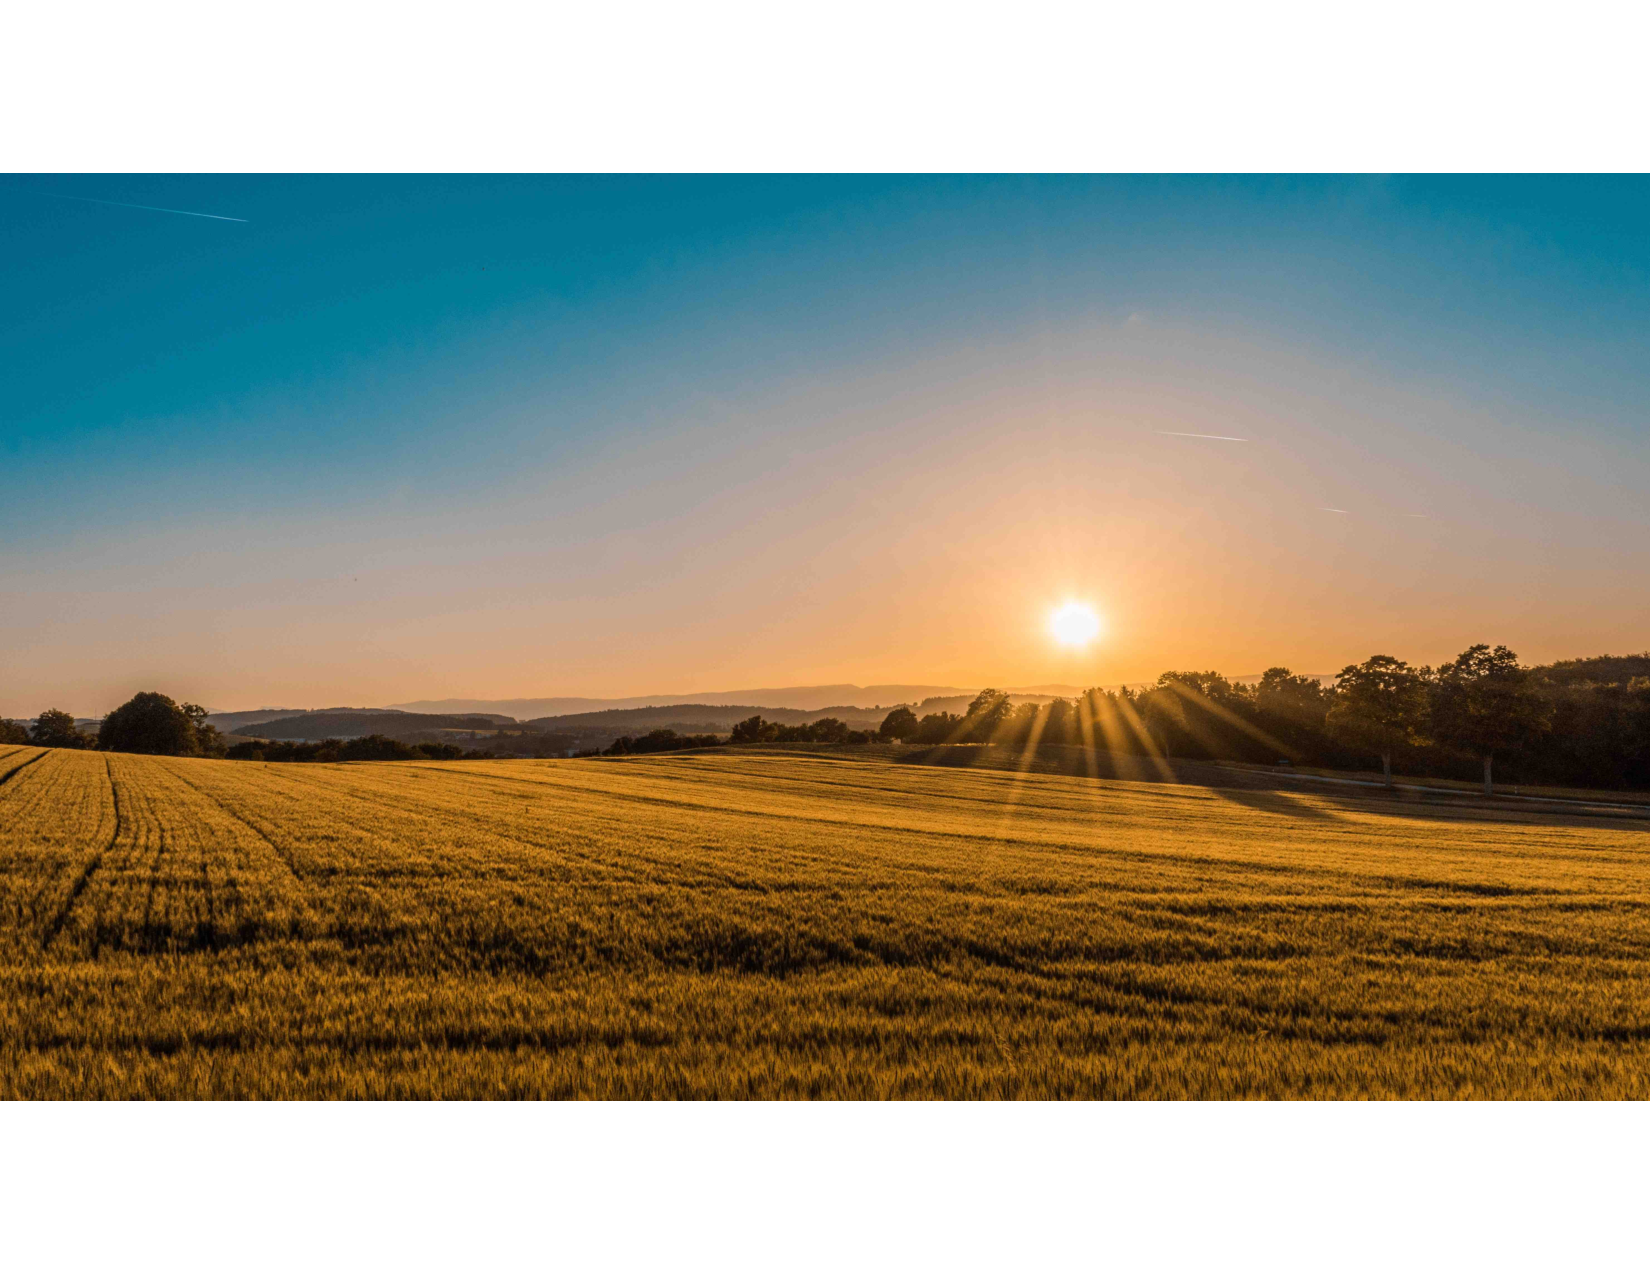
\includegraphics[clip=on,width=\columnwidth,height=0.6\textheight,keepaspectratio]{federico-respini-sYffw0LNr7s-unsplash}
\end{center}
\end{figure}

\vspace{10 mm }
\LARGE
\emph{Cloudy \& Associates} \\
\Large
\href{http://www.nublado.org}{www.nublado.org} \\
\normalsize
\today
\end{center}
\end{titlepage}

%%%%%%%%%%%%%%%%%%%%%%%%%%%%%%%%%%%%%%%%%%%%%%%
% page with one figure and boilerplate text
\clearpage
{\small
\noindent
{\em Software:} Copyright \copyright\ 1978-2022 Gary J. Ferland and others. All rights reserved.

\vspace{1em}

\noindent
The software described in this documentation (\Cloudy) is subject
to a FreeBSD-style software license
contained in the file \cdFilename{license.txt} in the
root directory of the distributed files.
The list of co-authors is given in the file
\cdFilename{others.txt} in the same directory.
Use of this program is not restricted provided each use is
acknowledged upon publication.
The bibliographic reference to this version of \Cloudy\ is
``version xx.xx
of the code last described \citet{CloudyReview}.''
The version number, shown here as ``xx.xx'', should be
given.
This version number, along with a complete citation,
can be found by executing the code with the 
\cdCommand{print citation} command included in the input script.

\vspace{1em}

\noindent
\Cloudy\ is an evolving code.
You should confirm that you have the most recent
version of the code by checking the web site
\href{http://www.nublado.org}{www.nublado.org}.
The code has a
\href{https://cloudyastrophysics.groups.io}{discussion board} with emailing list.
This will have announcements of any updates to the code.\par

\vspace{1em}

\noindent
Portions of the documentation have been published, and are copyrighted by, the
American Astronomical Society, the Astronomical Society of the Pacific, and
the Royal Astronomical Society. The remainder of the documentation is subject
to the following FreeBSD format documentation license:

\vspace{1em}

\noindent
{\em Documentation:} Copyright \copyright\ 1978--2022 Gary J. Ferland and others. All rights reserved.

\vspace{1em}

\noindent
Redistribution and use of the documentation (all parts of \Hazy\ and the
Quick Start Guide) in source (\LaTeX) and `compiled' forms (PDF, PostScript,
HTML and so forth) with or without modification, are permitted provided that
the following conditions are met:

\begin{enumerate}
\item
Redistributions of source code (\LaTeX) must retain the above copyright notice,
this list of conditions and the following disclaimer as the first lines of
the file \cdFilename{license\_doc.txt} in the root directory unmodified.
\item
Redistributions in compiled form (converted to PDF, PostScript, XML, HTML and
other formats) must reproduce the above copyright notice, this list of
conditions and the following disclaimer in the documentation and/or other
materials provided with the distribution.
\end{enumerate}

\noindent
{\em This documentation is provided by the \Cloudy\ project ``as is'' and any express
or implied warranties, including, but not limited to, the implied warranties
of merchantability and fitness for a particular purpose are disclaimed. In no
event shall the  \Cloudy\  project be liable for any direct, indirect, incidental,
special, exemplary, or consequential damages (including, but not limited to,
procurement of substitute goods or services; loss of use, data, or profits; or
business interruption) however caused and on any theory of liability, whether
in contract, strict liability, or tort (including negligence or otherwise)
arising in any way out of the use of this documentation, even if advised of
the possibility of such damage.}\par
}

\vspace{5mm}
\noindent
{\small
{\em Cover image:}
The dawn of a new day, representing Cloudy's migration between
development platforms and new development plans.
Photo by
\href{https://unsplash.com/@federicorespini}{Federico Respini} on
\href{https://unsplash.com/license}{Unsplash}.
}
\clearpage

%%%%%%%%%%%%%%%%%%%%%%%%%%%%%%%%%%%%%%%%%%%%%%%
% table of contents page - only include top two levels
\tableofcontents
\listoffigures
\listoftables

\clearpage
\mainmatter
% proofed 1 - read over latex file, remove dead xrefs,
% include figures, make xregs to figs and tables live
% NB the equations have not been checked
% proofed 2 - print document and read in detail
\chapter{INTRODUCTION}
% !TEX root = hazy1.tex

\section{Overview}

\noindent \Cloudy\ is a microphysics code.
It is designed to simulate physical conditions within clouds
ranging from the intergalactic
medium to the high-density LTE and STE limits.
The range of temperatures extends from the CMB temperature
up to \TEMPLIMITHIGH\ and the physical state
ranges between fully molecular to bare nuclei.
It predicts the thermal, ionization, and chemical structure
of a cloud which lies with these limits, and
predicts its observed spectrum.

This document describes the input, output,
and assumptions for the code.
It fully defines the commands used to drive the
program.
Part 2 gives details about the program
structure, its output, the computational environment, and how to call \Cloudy\
as a sub-program of other programs.
The methods, approximations, and assumptions used by \Cloudy\ are
outlined in Part 3 of this document, although this part, like \Cloudy\ itself,
is still under construction.
The \emph{Quick Start Guide} summarizes these
three volumes and gives a general overview of the simulations.

Many environments are encountered in which dilute gas is heated and
ionized by the radiation field striking the gas.  Under these
circumstances it is possible to predict the physical conditions (that
is, the distribution of ionization, density, and temperature) across
the cloud, and its resulting spectrum, in a unique and self-consistent
manner.  This is done by simultaneously solving the equations of
statistical and thermal equilibrium, equations that balance
ionization-neutralization processes, and heating-cooling processes,
respectively.  The graduate text \citet[hereafter
AGN3]{Osterbrock2006} describe the physics governing such environments
and \citet{Ferland2003} provides additional details on current
research topics.

The instructions for downloading and
setting up the code are on the web site
\href{http://www.nublado.org}{www.nublado.org}.
We maintain a discussion board at
\href{https://cloudyastrophysics.groups.io}
{cloudyastrophysics.groups.io}
where questions can be posted.

\section{What must be specified}

\noindent
One powerful asset of photoionization analysis is the large number of
observables resulting from only a few input parameters.
Intensities of a very large number of spectral lines\footnote{
There is no limit to the number of spectral lines that the code can
compute because there is no limit to the number of levels of atoms of the
H-like (\hO, \heplus, etc) and He-like (\heO, Li$^+$, etc)
isoelectronic sequences.
Processor speed and memory limit the simulation to a few million lines in
most applications with today's computers, however.}
are predicted by \Cloudy.  These result
from the specification of only a) the shape and intensity of the external
radiation field striking a cloud,
b) the chemical composition and grain content of the gas, and c) the geometry
of the gas, including its radial extent and the dependence of density on
radius.  The following subsections describe the general philosophy of the
specification of each.

\subsection{Incident radiation field}

\noindent Both the shape and intensity of the external radiation field striking the cloud
must be specified.
Often this is the region's only source of heat and
ionization.
Different commands are usually used to specify the external radiation field
shape and intensity, although a few commands specify both.

\begin{description}

\item[Shape of the external radiation field]
The shape of the spectral energy distribution (SED)
should be fully specified between a frequency
of \emmmhz\ $(\lambda \approx$ \emmcm\ -- this is the lowest
frequency observable with LOFAR) and an energy
of \egamry\ $(h\nu =$ \egamrymev)
if possible.\footnote{
In much of the following discussion photon energies will
be given in Rydbergs.  The ionization potential of hydrogen is nearly 1
Rydberg.  See the discussion in Part 2 of this document for an exact
definition and how to convert the Rydberg to other units.}
A physically-motivated radiation field spanning the full energy range
should be specified if possible.
This can be specified as a fundamental
form (such as blackbody emission, optically thin bremsstrahlung emission,
or a power law with optional exponential cutoff), interpolated from tables
of points, or as the radiation field transmitted through a cloud and
predicted by previous calculations.
Additionally, a set of built-in radiation fields
(for instance, emission from many model atmospheres, the observed
Crab Nebula spectral energy distribution (SED), or several typical AGN SEDs) can be specified as look-up tables.

\item[Intensity or luminosity of the external radiation field]
The intensity of the external radiation field striking the
cloud must be specified.
This can be given either as the flux striking a unit surface
area of cloud or as luminosity  radiated by the central object into $4\pi$~sr.
The code must be able to derive the flux of photons (cm$^{-2}$ s$^{-1}$) striking
the illuminated face of the cloud.
There are many commands that set these.
Two cases, the intensity and luminosity cases, can be used to
set the strength of the radiation field.
These are described in the next Chapter.

\item[Combining several radiation fields]
Up to 100 different radiation fields can be included as part of
the total field striking the cloud.
There must be exactly the same number of shape and luminosity
specifications.
The code will stop if there are not.

\end{description}

\subsection{Chemical Composition}

\noindent The program considers the lightest \LIMELM\ elements in detail.
Grains are
not part of the default composition but can be included.
All stages of
ionization are treated, and all published charge transfer, radiative
recombination, and dielectronic recombination processes are included as
recombination mechanisms.
Photoionization from valence and inner shells
and many excited states, as well as collisional ionization by
both thermal and supra-thermal electrons, and charge transfer, are included as ionization mechanisms.
The chemistry includes many molecules and will go to the fully
molecular limit (H in \htwo\ and C or O in CO).
Although the default composition
is solar several other standard mixtures can easily be specified and an
arbitrary composition can be entered.

\subsection{Geometry}

\noindent The geometry is always 1D spherical but can be made effectively plane
parallel by making the inner radius much larger than the thickness of the
cloud.  The default is for the gas to have constant density and to fully
fill its volume
Other pressure laws and strongly clumped clouds can be computed as well.

\Cloudy\ normally assumes an \cdTerm{open geometry},
or one in which the gas has
a very small \cdTerm{covering factor}
(these terms are defined in the following chapter
and in section 5.9 of AGN3).
This can be changed with
the \cdCommand{sphere} (see section \ref{sec:CommandSphere}) command which sets the covering factor
to a large enough value for light escaping
the cloud in the direction towards the central object to always interact
gas on the other side.
This is a \cdTerm{closed geometry}.
Line photons which
cross the central hole interact with line-absorbing gas on the far side
if \cdCommand{sphere static} is set but do not interact (because of a Doppler shift
due to expansion) if \cdCommand{sphere expanding} is set.
This case is the default when \cdCommand{sphere} is specified.

\subsection{Velocity Structure}

\noindent \Cloudy\ normally assumes that only thermal motions broaden spectral lines and that there is no internal velocity structure.
These assumptions can be changed.
A component of microturbulence can be added with the
\cdCommand{turbulence} command.
A flow can be computed with the \cdCommand{wind} command.

\section{The input deck}

\noindent \Cloudy\ is driven by a set of command lines.
These normally reside in a small input file which the code reads
when it starts.
The commands are four-letter keywords (either
upper or lower case) followed by free-format numbers that
may be mixed with letters.  The input is dependent on case for items
within quotation marks \verb|"|, such as file names (although the
case of filenames may then be ignored on some operating
systems).  Where the names of 
molecular species are specified, these will often need to be in quotation
marks, so that, for example, carbon monoxide (CO) and cobalt (Co) can be
distinguished.

When \Cloudy\ is executed as a stand-alone program standard input
(\cdFilename{stdin}) is read for input and standard output
(\cdFilename{stdout}) is used for output.  It may also be run using
commands stored in an text input file.  As an example, create a small
file (say, called \cdFilename{simple.in}) containing the following
lines:

\begin{verbatim}
title example input
hden 5 # log of hydrogen density, cm^-3
blackbody 5e4 K # spectral shape is a 50000K blackbody
# intensity of blackbody is set with
# ionization parameter so starting radius is not needed
ionization parameter -2
\end{verbatim}
Suppose that the code has been compiled to create the executable \cdFilename{cloudy.exe}.
Then, the model described by the parameters in this input file could be
computed by typing the following at the command prompt:
\begin{verbatim}
cloudy.exe -r simple
\end{verbatim}
Note that on many Linux systems the command will have to be written as
\begin{verbatim}
./cloudy.exe -r simple
\end{verbatim}
for system security.  
The file \cdFilename{simple.in} will be read for input and the output will be in the file
\cdFilename{simple.out}.  

The \href{http://www.nublado.org}{www.nublado.org} web site has many more details
about running this version of \Cloudy\ in the page
\href{https://gitlab.nublado.org/cloudy/cloudy/-/wikis/RunCode}{RunCode}.

It is also possible for a larger program to drive \Cloudy\ directly by
treating it as a subroutine. 
See \href{https://gitlab.nublado.org/cloudy/cloudy/-/wikis/RunCode}{RunCode} for more details.

\section{What is computed and reported}

The code creates an output file as the model is computed.
The program begins by echoing the input commands (after stripping hidden
comments, see Sect.~\ref{sec:CommentsInInput} for details).  Comments are
always ignored by the parser.  The input stream ends with either a blank line or
the end-of-file.  Some properties of the incident radiation field, such
as luminosity and number of photons in certain frequency ranges, are then
printed.

\Cloudy\ works by dividing a cloud into a set of thin concentric shells
referred to as zones. The zones are chosen to have thicknesses that are
small enough for the physical conditions across them to be nearly constant.
Adaptive logic continuously adjusts the physical thicknesses of these shells
to ensure this.  Typically $\sim$100 to 200 zones are computed in an optically
thick model of an H~II region.  The physical conditions in the first and
last zones are always printed and intermediate zones may be printed if needed
(this is governed by the \cdCommand{print every} command).
The output for each zone begins with a line giving the zone number, its
electron temperature, the distance from the center of the spherical nebula
to the center of the zone, and some other properties of the solution.  The
next line gives the relative contributions of various emission lines to
the radiation pressure if this amounts to more than 5\% of the gas pressure.
The remaining lines of output give the relative populations of
ionization stages of the other elements.
Many details about the conditions within the zone are
intermixed with these relative populations.

After the zone calculations are complete and the model is finished the
code will explain why the calculation stopped.  It is very important to
confirm that the calculation stopped for the intended reason.  Some warnings,
cautions, or notes about the calculation may also be printed.  The code
is designed to be autonomous and self aware.  This self checking will ensure
that its range of validity is not exceeded. It will complain if it goes
outside its range of validity, if it feels that some parameter has been
incorrectly set, or if something surprising has happened during the
calculation.  This is an essential core feature of the code since it is
now often used to generate grids of thousands of models, making it impossible
to validate individual models by hand.

The final print out begins with a recapitulation of the entered commands
followed by the predicted emission-line spectrum.  The first two columns
of the emission-line spectrum give an identifying label and wavelength for
each spectral line.  The third column is the log of the luminosity [erg
s$^{-1}$] or intensity [erg cm$^{-2}$ s$^{-1}$] of the emission line, and the last column
gives its intensity relative to the reference line.
The reference line is H$\beta$ by default and other emission lines
can be chosen with the \cdCommand{normalize} command.
The third column will be either the luminosity or intensity.
The luminosity (energy radiated by a shell of
gas covering $\Omega$ sr of the central object) is predicted if the incident radiation field is
specified as a luminosity.  The line intensity $4\pi J$ (the energy emitted per
square centimeter of the gas slab) is predicted if the incident radiation field is specified
as an intensity.  If the geometry is spherical but the incident radiation field is specified
as an intensity then the line intensities will be expressed per unit area
at the inner radius.  Only the strongest emission lines are printed; the
relative intensity of the weakest line to print is adjusted with the
\cdCommand{print faint} command.

The last pages of the output gives some averages of the ionization
fractions over the slab, the optical depths in various lines and continua,
and other properties of the nebula.

There is a vast amount of information that is computed but not given
in the standard output file.  Special output files are created with the
\cdCommand{save} commands described below.
      
\chapter{DEFINITIONS}
% !TEX root = hazy1.tex

\section{Overview}

This section defines many of the quantities used by \Cloudy.  I try to
follow standard notation, such as that used by \citet{Mihalas1978} or AGN3.
Other parts of this document goes into many of these quantities in greater detail.

This document has the following typographic conventions;
\cdFilename{filename},
\cdTerm{variable},
\cdCommand{command},
\cdTerm{jargon},
\experimental\ experimental commands,
\cdVariable{variable name},
and \cdRoutine{routine name}.

\section{Radiation fields}

Figure \ref{fig:radiation_fields} shows several of the
radiation fields computed in the calculation.
%2.1
\begin{figure}
\centering
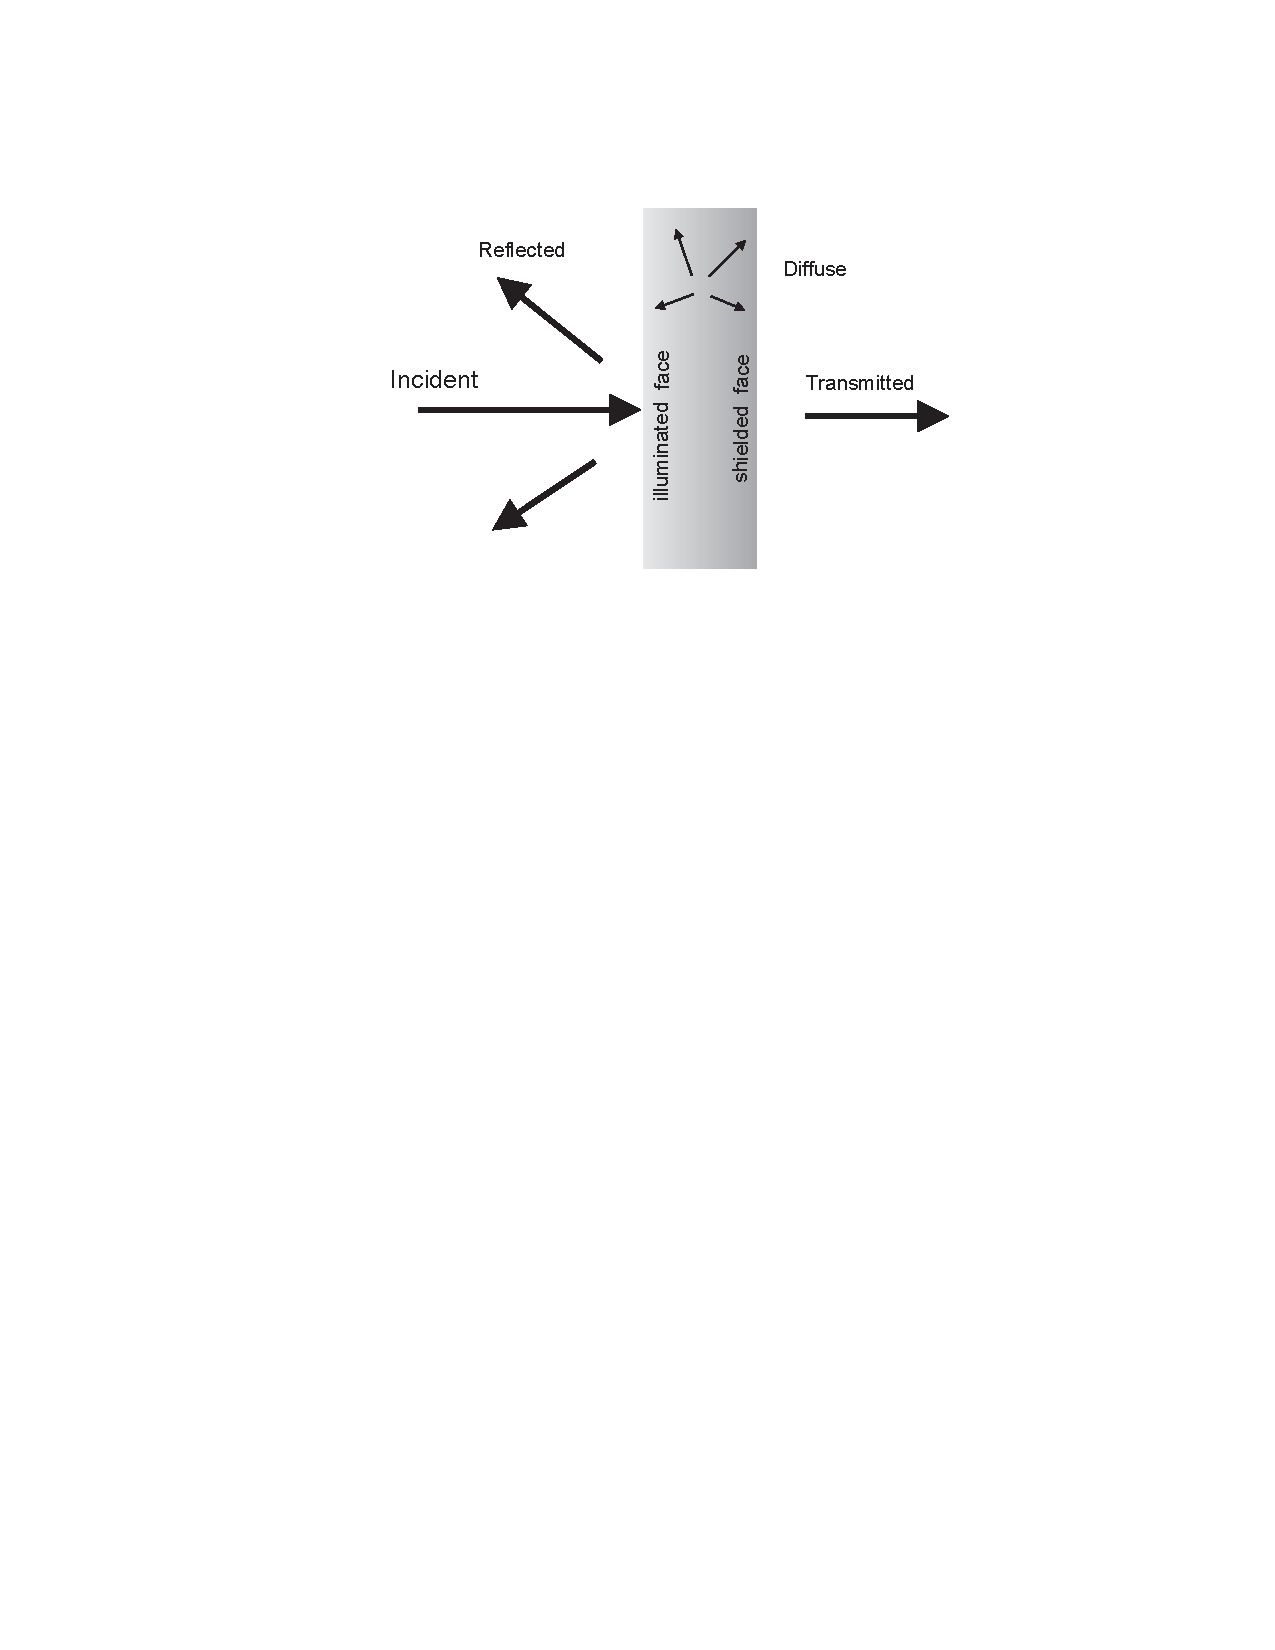
\includegraphics{radiation_fields}
\caption[Contributors to total radiation field]{Several of the radiation fields that
enter in the calculations.}
\label{fig:radiation_fields}
\end{figure}

\subsection{Incident radiation field}

The \cdTerm{incident radiation field} is the external radiation field emitted by the central
object that strikes the \cdTerm{illuminated face} of the cloud.
It is specified in
the commands that set up the calculation.
Often the incident field
is the only energy source for the cloud.
As the incident radiation field is
transmitted through the cloud it is diminished by extinction.

\subsection{Diffuse radiation field }

The \cdTerm{diffuse radiation field} (often referred to as the
diffuse fields) is the radiation field emitted by gas and grains within
the nebula.  Examples include the Lyman, Balmer, or two-photon continua
emitted by hydrogen.  These fields are very nearly isotropic and can be
significant sources of ionizing radiation under some circumstances.

The main difference between the calculation of a stellar atmosphere and
a photoionized cloud is in the treatment of the diffuse fields.
The gas
albedo, which gives the relative probability of a photon being scattered
versus being absorbed, is generally small in a nebula.
As a result, the
diffuse fields must be far weaker than the attenuated incident continuum
since the second is usually the cloud's only real energy source.
The total radiation field is usually dominated by the attenuated
incident radiation field.
By contrast
in a stellar atmosphere the nearly isotropic diffuse field usually dominates
the local intensity.
As a result the diffuse fields can be treated by lower
order approximations in a photoionized cloud than in a stellar atmosphere.

\subsection{Transmitted radiation field}

The \cdTerm{transmitted radiation field} is the net
emission emergent from the shielded
face of the cloud.
It includes both the \cdTerm{attenuated incident} and
the \cdTerm{diffuse} radiation fields.

\subsection{Reflected radiation field}

The \cdTerm{reflected radiation field} is the emission
from the illuminated
face of the cloud back into the direction towards
(i.e., within $2\pi$~sr of)
the source of the external field.
The reflected field is the result
of both backscattered incident radiation and diffuse emission emitted from
the cloud towards the source of ionizing radiation.
This component is only
computed for an \cdTerm{open geometry} (defined below).

Figure \ref{fig:incident_reflected} shows a plot of the incident and
reflected radiation fields for the Compton reflector in an AGN.
This is a large column-density cloud, $N(\mathrm{H}) = 10^{23.75}$
cm$^{-2}$, illuminated by a $f_v\propto v^{-1}$ power law.
The incident radiation field is shown as a
dashed line and the reflected radiation field, obtained from the \cdCommand{save continuum} command),
is the solid line.
The Compton reflector's peak at X-ray
energies is clearly shown.

\begin{figure}
\centering
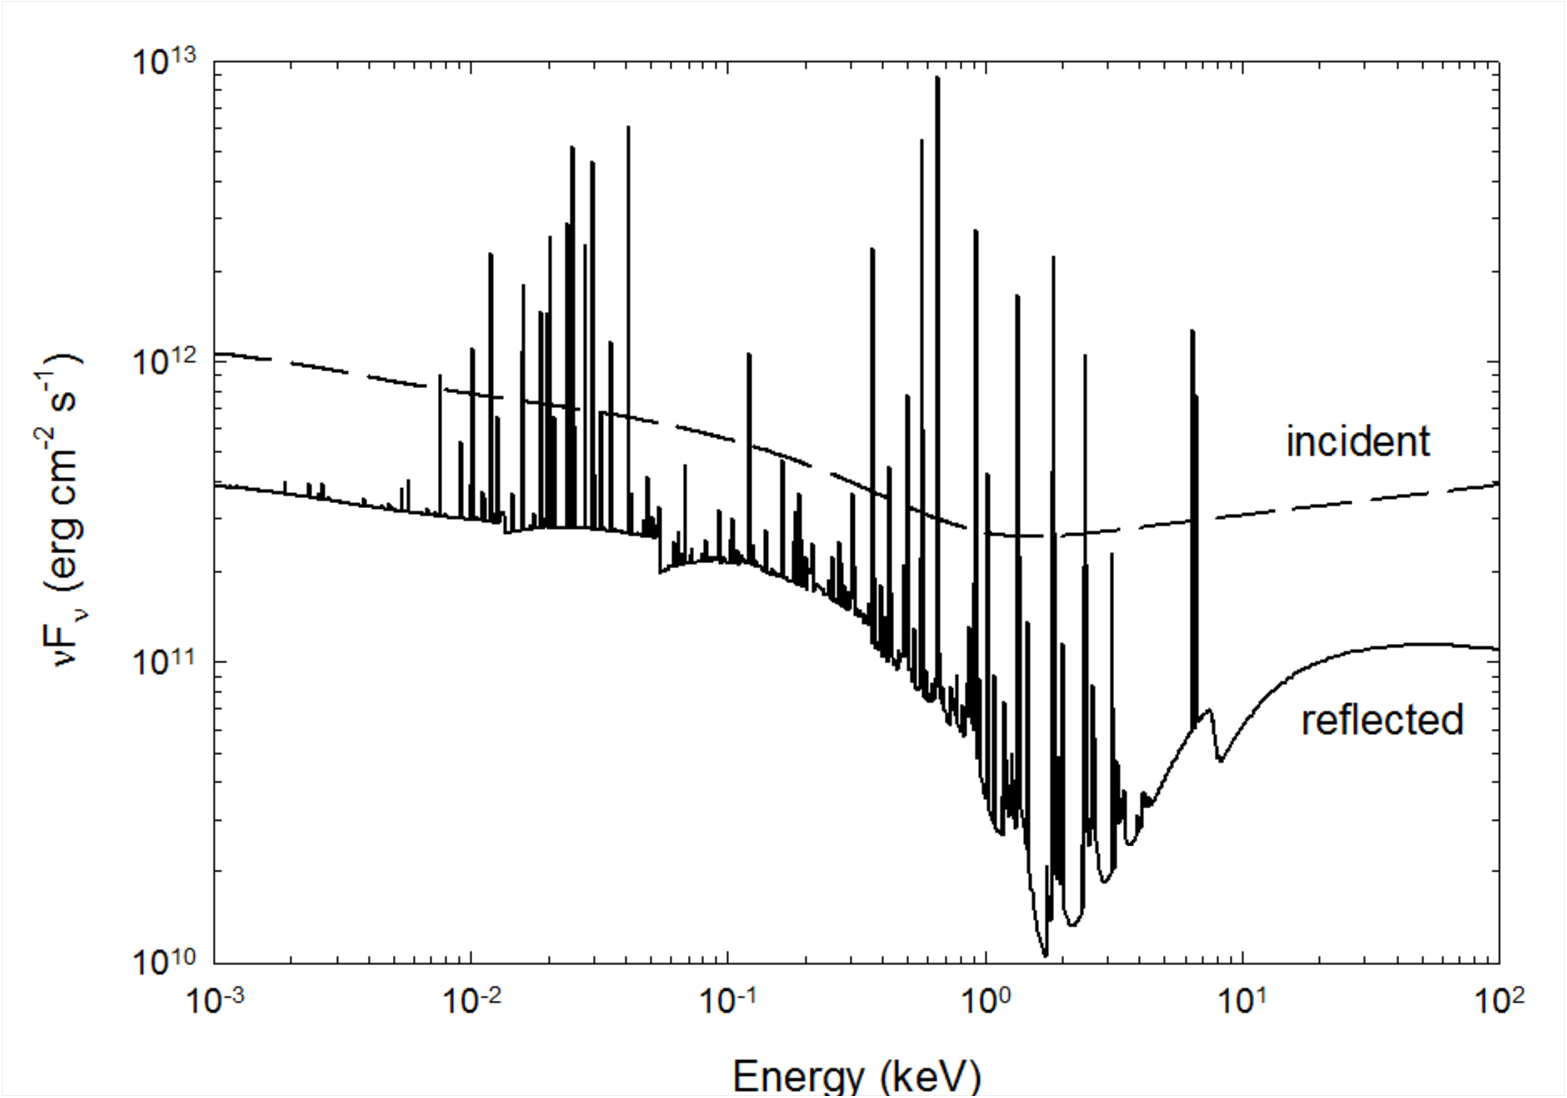
\includegraphics[scale=0.7]{incident_reflected}
\caption[Incident and reflected radiation field]{This incident (dashed) and reflected (solid)
radiation fields,
as computed by agn\_blr\_albedo.in in the test suite.}
\label{fig:incident_reflected}
\end{figure}

\section{Geometry}

In the simplest case the geometry is spherical, or plane
parallel if the inner radius is much larger than the thickness of the
cloud.
The summary at the end of the calculation will
say whether the geometry was plane parallel  (the ratio of the thickness
to the inner radius, $\Delta r/r_o < 0.1$), a thick shell ($\Delta r/r_o <
3$), or spherical
($\Delta r/r_o \ge 3$).

Complex geometries are done by using Cloudy to compute volume elements
within a much larger cloud.
An example is the Cloudy\_3D code,
available from 
\href{http://sites.google.com/site/cloudy3d/}{sites.google.com/site/cloudy3d}
and described in \citet{MorissetCloudy3D06}
and \citet{MorissetStasinskaCloudy3D08}.
Cloudy\_3D was used to compute
the images shown on the cover and in Figure~\ref{fig:Cloudy3D}.
The RAINY3D code is another example 
\citep{MoraesDiazRAINY09}.

\begin{figure}
\centering
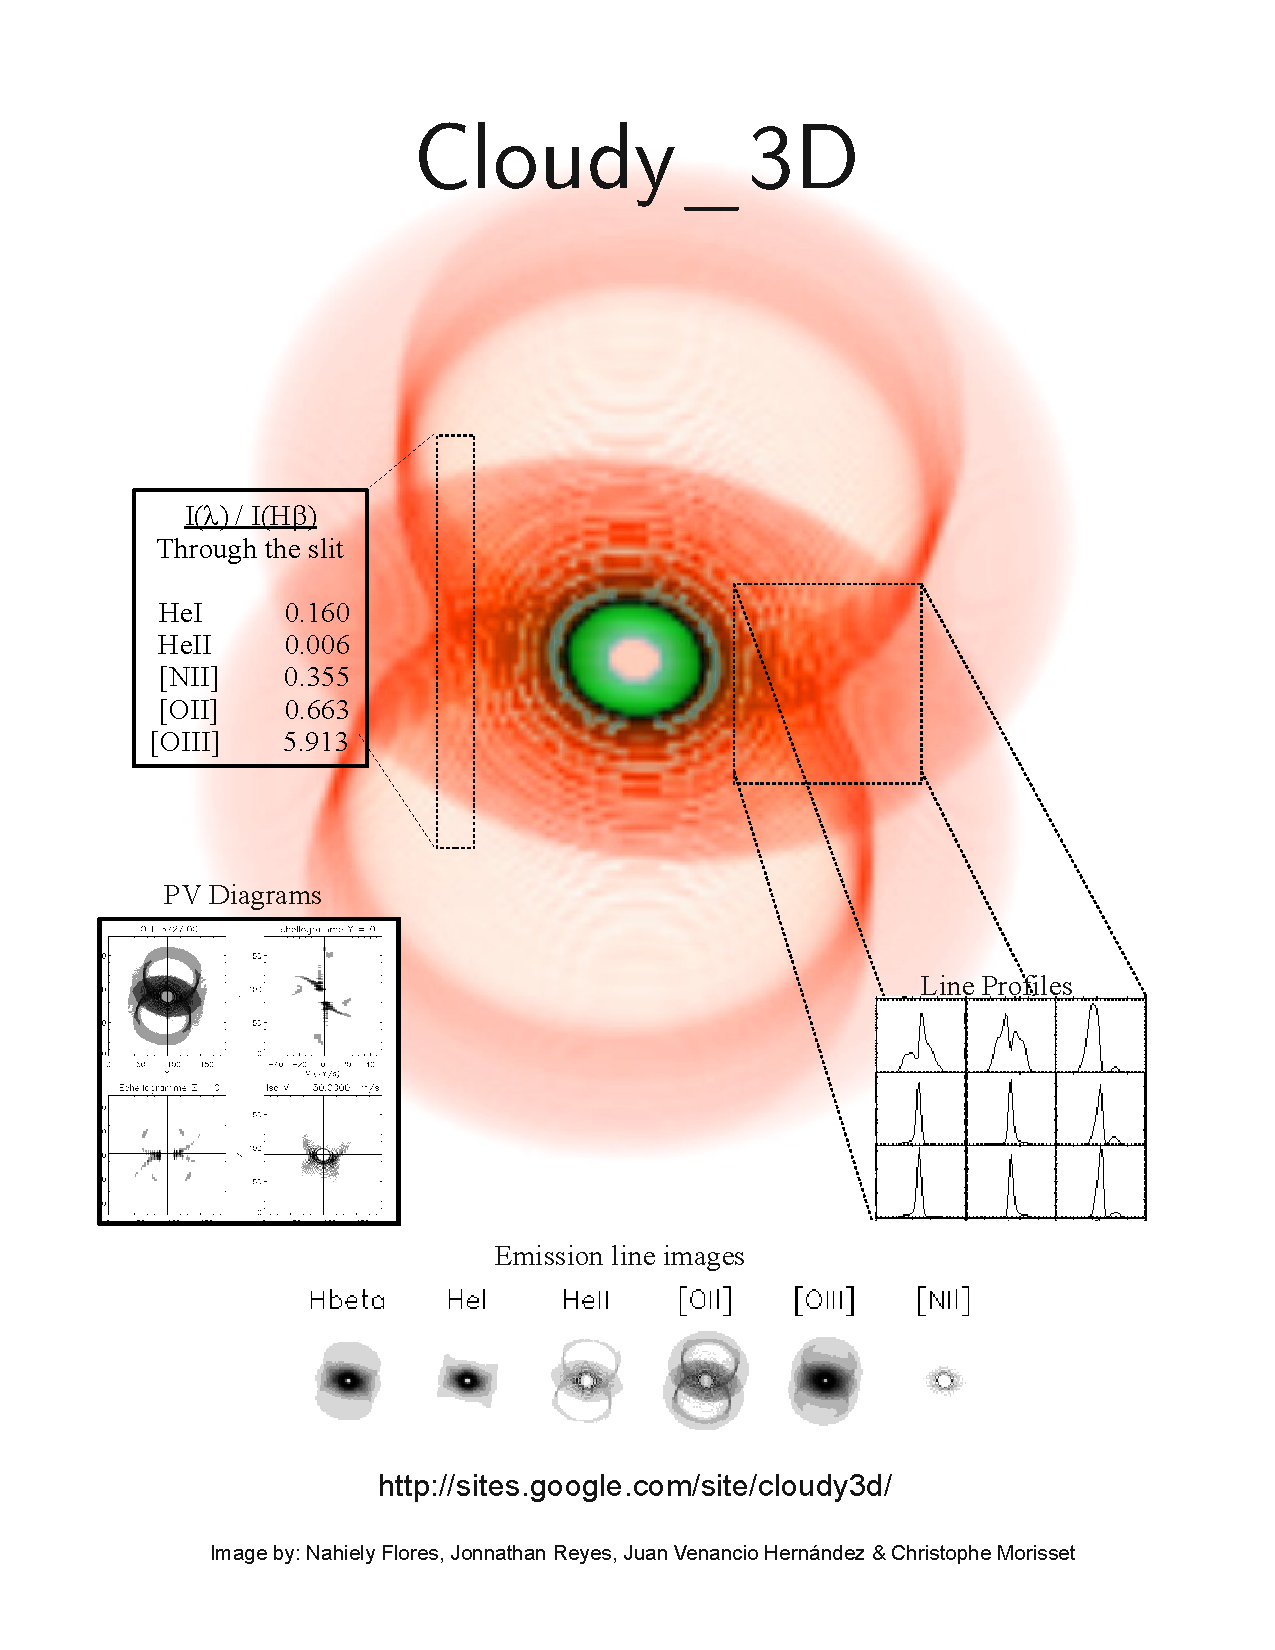
\includegraphics[width=\columnwidth]{posterhazy02}
\caption[Cloudy\_3D simulation of a planetary nebula]
{A 3-color image of a Hourglass-type nebula, 
obtained by running Cloudy 3D.
Colors are [\nii ] (orange) and [\oiii ] (green) emission. 
Emission line profiles are shown for [\nii ] lines. 
Intensities through any given slit can be obtained. 
Position-velocity diagrams are obtained as well as
channel maps, for any line. 
Emission line surface brightness maps are
also available for any line computed by \Cloudy. 
Statistical tools to
analyze emission line properties are also provided.}
\label{fig:Cloudy3D}
\end{figure}

\subsection{Illuminated and shielded faces of the cloud}

The side of the cloud facing the source of the external radiation field
is the \cdTerm{illuminated face} of the cloud.
The opposite side, in shadow, is the \cdTerm{shielded face} of the cloud.  
The illuminated face is generally
hotter and more highly ionized than the shielded face.
In nearly all cases the calculation starts at the illuminated face and stops at the shielded face.

\subsection{Depth and radius}

Figure \ref{fig:GeometryOpenClosed} shows two possible geometries
and some terms used to describe them.
The \cdTerm{radius} is the distance from the center of symmetry,
usually the center of the central object, to a given point.
The \cdTerm{depth} is the distance
between the illuminated face of the cloud and a point within the cloud.
The \cdTerm{inner radius} is referred to as $r_o$,
the depth is $\Delta r$, and the \cdTerm{current radius} is $r$.
The depth or radius for a zone is the distance to the center of the zone.

\begin{figure}
\centering
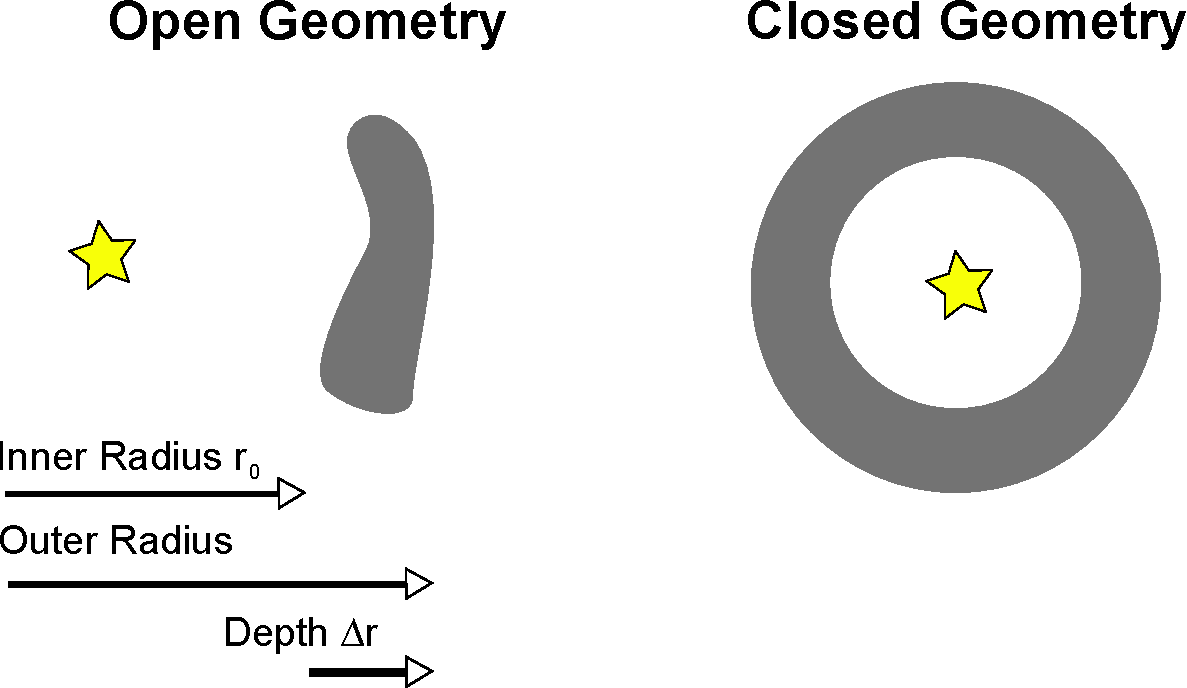
\includegraphics[scale=0.5]{GeometryOpenClosed}
\caption[Open and closed geometries]
{This figure shows the two limiting cases that can be assumed.
The star is the source of ionizing radiation and the shaded area represents
the cloud. An open geometry is the default, and a closed geometry will be
computed if the \cdCommand{sphere} command is entered.}
\label{fig:GeometryOpenClosed}
\end{figure}

\subsection{Covering factor}

The \cdTerm{covering factor} is the fraction of $4\pi$~sr
covered by gas, as viewed
from the central source of radiation.
It is normally written as $\Omega/4\pi$ (AGN3 Section 5.9),
has the limits $0\le\Omega /4\pi\le 1$,
and is the fraction of the
radiation field emitted by the central object
that actually strikes nebular gas.
\cdTerm{Line luminosities} give the total energy emitted by
a shell covering
$\Omega$~sr while \cdTerm{line intensities} give
the energy emitted per unit area of cloud.
Line luminosities scale nearly linearly with increasing covering factor
while line intensities are only weakly dependent on it.

\subsection{Open vs. closed geometry}
\label{sec:GeometryOpenClosed}

Two limiting cases, referred to as \cdTerm{open} and \cdTerm{closed}, can be identified
for the geometry and its influence upon the calculations.
Figure \ref{fig:GeometryOpenClosed} shows
examples of both.
The covering factor determines which is the best
approximation.
The choice mainly affects the transfer of the diffuse fields
and has only second-order effects on predicted quantities.

\begin{description}
\item[Open geometry.]
An \cdTerm{open} geometry is one in which the covering factor
of the gas is small. All radiation that escapes from the illuminated face
of the cloud, towards the source of continuous radiation, then escapes from
the system without further interaction with gas. This is thought to be
the case in, for example, the broad-line region of active nuclei or a blister
H~II region.  In this case L$\beta$ and higher hydrogen Lyman lines and ionizing
radiation produced by recombinations can escape from the nebula.  This
geometry is the default and will be assumed if the \cdCommand{sphere} command is not specified.

\item[Closed geometry.]
Emission-line gas covers ${\sim}4\pi$ sr as seen by the central
object in a \cdTerm{closed} geometry.
The central object is small relative to
the nebula then all diffuse fields which escape from the illuminated face
of the cloud in the direction towards the central object will go on to strike
the far side of the nebula.
This geometry is implicitly assumed in most
calculations of planetary nebulae and \hii\ regions.
This geometry will be
assumed if the \cdCommand{sphere} command is entered.

\item[Static vs. expanding.]
The sphere command has two optional arguments,
\cdCommand{static} and \cdCommand{expanding}.  This determines how emission-line photons which cross
the central hole and strike the far side of the shell interact with the
gas.  The \cdCommand{static} option says to assume that the shell is stationary so that
all lines interact across the nebula.  In this case hydrogen Lyman line
interaction should ensure that Case~B is reached (AGN3 Section 4.2).  If
the nebula is expanding then the continuum photons that cross the central
hole will interact with gas on the far side but the expansion velocity of
the shell ensures that diffuse line photons do not.  In this case the
\cdCommand{expanding} option should be set.  This second case is the default
when \cdCommand{sphere}
is specified with no options.

\emph{Don't panic!}  These geometrical considerations (open vs closed, static
vs expanding) make only second-order differences in the predicted
emission-line spectrum, generally at the ${\approx}10$\% level, largely because of
the different treatments of the radiative transfer of the diffuse fields.
If you are concerned about which geometry to use, try both, and compare
the results.  The differences are usually small.
\end{description}

\subsection{Filling factor}

The \cdTerm{filling factor} $f(r)$ accounts for clumping
of emission-line gas.
When a filling factor is set the hydrogen density is the density within
regions containing gas while surrounding regions are assumed to be a vacuum.
The specific effects of a filling factor are described by \citet{Osterbrock1959} and in AGN3 section 5.9.

\subsection{Hydrogen density}

The \cdTerm{hydrogen density} $n(\mathrm{H})$ is the
total hydrogen density given by
\begin{equation}
n(\mathrm{H}) = n(\mathrm{H}^0) + n(\mathrm{H}^+) + 2n(\mathrm{H}_2)+\sum_{other}
n(\mathrm{H}_{other})\ [\mathrm{cm}^{-3}]
\end{equation}
where $n(\mathrm{H}_{other})$ represents H in all other hydrogen-bearing molecules.

\subsection{Column densities}

The \cdTerm{hydrogen column density} $N$(H) is given by
\begin{equation}
N(\mathrm{H})= \int n (\mathrm{H})\, f(r) \, dr \ [\mathrm{cm}^{-2}]
\end{equation}
where $f(r)$ is the filling factor.   I try to consistently use lower case
$n$ for a volume density (cm$^{-3}$) and an upper case $N$ for
a column density (cm$^{-2}$).

\subsection{Matter-bounded and radiation-bounded geometries}

Two limiting cases for the hydrogen-ionization structure of a cloud exist.

\begin{description}
\item[Matter-bounded geometry.]
The cloud is said to be matter bounded if
the outer limit to the \hplus\ region is marked by the
outer edge of the cloud.
In this case the cloud is ionized throughout
and is optically thin to the
incident radiation field.
In a matter-bounded cloud the intensity or luminosity
of an optically thin recombination line is set by
the product of volume and density
(called the emission measure $n^2V$, AGN3, Section 8.1) and is
not directly related to the luminosity of the ionizing continuum.

\item[Radiation-bounded geometry.]
The cloud is said to be radiation bounded
if the outer limit to the \hplus\ region is defined by
a hydrogen ionization
front so both warm ionized and cold neutral regions exist.
The \hplus\ region
is optically thick to the hydrogen-ionizing radiation
and has absorbed nearly all of it.
In this case the intensity or luminosity of a recombination
line is set by the luminosity of the ionizing continuum with
relatively little dependence on cloud properties.
\end{description}

\section{Intensity \& luminosity cases }
\label{sec:IntensityLuminosityCases}

The external radiation field is usually specified with
two different commands.
One specifies the shape of the incident radiation field.
A second command will set the brightness of the light.
\Cloudy\ must be able to deduce the flux of photons
[cm$^{-2}$ s$^{-1}$]
striking the illuminated face of the cloud.
There are two ways to specify the brightness of the external radiation field.

\subsection{Luminosity case}

If the brightness of the external radiation field is specified as a ``luminosity'',
the light radiated by the central object into $4\pi$~sr, then it is also
necessary to specify an inner or starting radius so that the flux of
photons can be derived.

The emission lines will be predicted as luminosities.
A covering factor will linearly change the luminosity of the entire spectrum
but will have only second order effects on relative intensities.

\subsection{Intensity case}

The external radiation field can be specified as an ``intensity'',
the energy
incident upon a unit area of cloud, with units
something like photons cm$^{-2}$~s$^{-1}$.
It is not necessary to specify a starting radius in the intensity case
although it is possible to do so.
Line intensities (energy emitted per
unit area of cloud, related to $4\pi J$)), are predicted in this case.

If the ``intensity'' of the external radiation field is set then a starting radius does not
need to be specified.
If the starting radius is not specified then an inner
radius of 10$^{30}$ cm is assumed.  A plane-parallel geometry usually results.
The predicted emission-line spectrum is then given in intensity units.
A starting radius may be specified and, if it is, then the resulting geometry
may be spherical, plane parallel, or a thick shell, depending on the ratio
of the outer to inner radii.  Both absolute and relative intensities of
lines have only second-order dependencies on the covering factor.

The word ``intensity'' appears in quotes since it is
not the $I$ or $J$ defined in radiative transfer texts, but rather the photon
or energy equivalent of $4\pi J$.

\subsection{The units of the predicted emission lines}

The units of the predicted emission-line spectrum are determined by the
units of the incident radiation field.
If the incident field is specified as a
luminosity then the spectrum will be given as the luminosity radiated by
a shell covering  $\Omega$~sr of the central object ($L_{line}, \mathrm{erg\,
s}^{-1}$).  Here $\Omega$ is the
angular coverage of the nebula so that $\Omega/4\pi$ (with a default value of unity)
is the covering factor (AGN3, Section 5.9).  If the
continuum is specified as an intensity then the spectrum will be the energy
radiated by a unit area of cloud into $4\pi$~sr $(4\pi J_{line}$, erg
cm$^{-2}$~s$^{-1}$).

\section{``Species'', how we specify atoms, ions, and molecules, and their spectra}
\label{sec:SpeciesDefine}

\subsection{Overview}
\Cloudy\ simulates gas ranging from fully ionized to molecular.
Nomenclature varies considerably between chemical, atomic, and plasma physics.
We adopted a nomenclature that tries to find a middle ground between
these different fields.

We refer to a particular atom, ion, or molecule as a ``species''.
A species is a baryon.  Examples are CO, \htwo, H$^+$, and Fe$^{22+}$.
Species are treated using a common approach, as much as possible.
Our naming convention melds a bit of each of these fields
because a single set of rules must apply to all species.

The species are taken from a number of databases and a large
number of commands control how they are used.
These commands are described in the Section beginning on page 
\pageref{sec:ControllingAtomicModels} below.
The commands controling output options for the species are
described in the Section starting on page
\pageref{sec:SaveSpecies} below.

A spectrum is a collection of photons.  Examples that might appear in the literature
are H~I or C~IV.  
It is not convenient to use these labels in computer input/output.
We adopted the following rules.

\subsection{How we specify species and spectra}

Some rules for how these are specified:

\begin{itemize}

 \item
 Labels are case sensitive, to distinguish between the
 molecule CO and the atom Co.
 
 \item
 At present we do not use \verb|_| to indicate subscripts, or \verb|^|
 to indicate  charge.

 \item
 Molecules are written pretty much as they appear in texts.
 \htwo, CO, and H$^-$ would be written as ``H2'', ``CO'', and ``H-''.

 \item 
 Atoms are the element symbol by itself.
 Examples are ``H'' or ``He''
and \emph{not} the atomic physics notation
 H$^0$ or He$^0$.
 
 \item 
 Ions are given by ``+'' followed by the net charge.
 Examples are ``He+2'' or ``Fe+22''
 and \emph{not} the correct atomic physics notation,
 He$^{2+}$ or Fe$^{22+}$.
 The latter would clash with notation for molecular ions.
 ``C2+'' indicates C$_2^+$ in our notation.
 
\item We use \^{} to specify isotopes, with \^{} and the atomic weight
  placed before the atom to which it refers.  For example,
  ``\^{}13CO'' is the carbon monoxide isotopologue $\rm ^{13}CO$.
  
\item The \cdCommand{save species labels all} (page \pageref{sec:SaveSpeciesLabels}) 
command will produce a file containing the full list of species labels.

 \item
 We follow a modified atomic physics notation for the spectrum.
 H~I, He~II, and C~IV are the spectra emitted by H$^0$, He$^+$, and C$^{3+}$.
 In atomic physics the notation ``H~I'' indicates a collection of photons while H$^0$ is a baryon.  
 Emission lines replace the Roman numeral with an integer.
 Examples are H~~1 $\lambda 4861$\AA, 
 He~2  $\lambda 4686$\AA,
 and C~~4  $\lambda 1549$\AA.
 
 The spaces between the element and integer are significant.
 The spectrum label fills four characters so there are two spaces within
H~~1, one  space within Si~2, and no spaces within Fe16.\footnote{
It is not safe to copy/paste these labels from the PDF file.
Tests show that only one space is rendered.  Try this experiment
with the H~~1.  Copy/paste it into a text editor like vi.  There will be one space.
The original LaTex was correct and had two.}

\item
To summarize, atomic hydrogen would be referenced as ``H'' while the L$\alpha$
line would be ``H~~I''.  The distinction is important because,
depending on how it is formed, L$\alpha$ can trace either
H$^0$ or H$^+$.

\item  The \cdCommand{save line labels} command
(page \pageref{sec:SaveLineLabels} will create a file
listing all spectral lines predicted by the code, along with a brief comment.
  
 \item
 The internal structure of a species, and associated cooling / emission, are computed
 using external databases, as described in the section beginning on
 page \pageref{sec:ControllingAtomicModels}.
 We use our own Stout database, along with the 
\href{http://www.chiantidatabase.org/}{Chianti}  
(\cite{Dere.K97CHIANTI---an-atomic-database-for-emission}; \cite{Landi2012})
and Lamda, the Leiden Atomic and Molecular
Database (\href{http://www.strw.leidenuniv.nl/~moldata/}{www.strw.leidenuniv.nl/~moldata/}, 
\citet{Schoier.F05An-atomic-and-molecular-database-for-analysis}) databases.

\item
Each databases has its own ``masterlist'' file that
specifies which models to use.
The masterlist file follows the notation used within the databases.
For Chianti and Stout, the internal structure of C$^{3+}$, which produces C~IV emission,
is called ``c\_4''.
The water molecule in Lamda is referenced as ``H2O''.

\item
If a particular species is specified in more than one masterlist file we will
use Stout if it exists, then Chianti, followed by Lamda.  

 \end{itemize}

\subsection{How we specify spectral lines}
\label{sec:SpecifySpectralLines}

Several commands require you to specify a list of spectral lines, either in
the input script or in a separate file. One example is the \cdCommand{save
  line list} command. In all cases the same format is used. You need to
specify exactly one spectral line on each input line, consisting of a species
label followed by a wavelength. If the species label is four characters or
shorter, you can type it {\it as is} in the first four columns of the input
line. If it is longer, it is mandatory that you surround the label with double
quotes. You may also use double quotes for labels that are four characters or
shorter, but this is optional. If you use double quotes, the string must start
in the first column. After the label you need to enter the wavelength. The
code assumes that wavelengths are in \AA ngstrom by default. You can also
supply wavelengths in micrometer or centimeter by appending a ``m'' or ``c''
directly after the number (i.e., there may be no spaces inbetween). Note that
the wavelength must start in the 5th column or later, even when the species
label is shorter than four characters. Nothing else may appear on the line
except a comment starting with a comment character as is shown in the examples
below. In general it is best to do a copy / paste of a line identification
from the \Cloudy\ output (e.g., the line list produced with the
\cdCommand{save line labels} command) but remember that species labels that
are longer than 4 characters {\em must} be enclosed in double quotes. Below we
show some examples of how you enter spectral lines.
\begin{verbatim}
o  3  5006.84 # green line of [O III], wavelength in Angstrom
CO   2600.05m # CO 1 -> 0 line, wavelength in micron
CO 2600.05m   # INVALID! wavelength starts in column 4!
"o  3" 834.5A # double quotes are optional here
"^13CO" 2719.67m # double quotes are mandatory here!
\end{verbatim}

\subsection{What species are you using?}

You can generate a report giving all species, the number levels in the model,
and the database used for the species,
by running \Cloudy\ with the following input;
\begin{verbatim}
test
species print
\end{verbatim}

You can generate a list of all species labels by running the following input deck:
\begin{verbatim}
test
save species labels "test.slab"
\end{verbatim}

You can generate a list of all emission lines by running:
\begin{verbatim}
test
save line labels "test.llab"
\end{verbatim}

The following is an example using species labels to report the column densities 
of several ions and molecules, together with the visual extinction:
\begin{verbatim}
save species column densities "test.col"
"e-"
"CO"
"H2"
"H"
"H+"
"*AV"
end of species
\end{verbatim}

\section{Air vs vacuum wavelengths}
\label{sec:AirVsVacuumWavelengths}
The convention in spectroscopy, dating back to 19$^{th}$ century experimental atomic physics,
is to quote line wavelengths in vacuum for  $\lambda < 2000$\AA\ and STP air wavelengths
for $\lambda \ge 2000$\AA.
The \cdCommand{print line vacuum} command, 
described on page \pageref{sec:CommandPrintVacuum},
tells the code to use vacuum wavelengths throughout.
The continuum reported by the family of \cdCommand{save continuum} commands,
described on page \pageref{sec:CommandSaveContinuum},
is always reported in vacuum wavelengths to avoid 
a discontinuity at 2000\AA.


     
\chapter{INTRODUCTION TO COMMANDS}
% !TEX root = hazy1.tex

\section{Overview}

This section introduces the commands that drive \Cloudy.
The following
chapters group the commands together by purpose.
Individual commands are
discussed after examples of their use.
This section begins by outlining
conditions that are assumed by default and then goes on to discuss the
various classes of commands (i.e., those that set the incident
radiation field, composition, or the geometry).

Keeping this document parallel with the code is a very high priority.
In case of any confusion, please consult the original source.
The commands are
parsed by the series of routines that have names beginning with
\cdRoutine{``parse''.}
The list of routines can be seen by listing the files \cdFilename{parse*.cpp}.
The second
half of the name indicates the command that is parsed by that routine.

\Cloudy\ is designed so that a reasonable set of
initial conditions to be assumed by default so that
a minimum number of commands are needed to drive it.
These default conditions are summarized
in Table \ref{tab:DefaultConditions},
which also lists the
commands that change each assumption.

\begin{table}[t]
\centering
\caption{\label{tab:DefaultConditions}Default Conditions}
\begin{tabular}{l l l }
\hline
Quantity& Value& Command\\
\hline
Default inner radius& $10^{30}$ cm& \cdCommand{radius}\\
Default outer radius& $10^{31}$ cm& \cdCommand{radius}\\
Highest allowed temperature& \TEMPLIMITHIGH\\
Stop calculation when
$T$ falls below this value& \TEMPSTOPDEFAULT& \cdCommand{stop temperature}\\
Relative error in
heating-cooling balance& 0.005& \cdCommand{set temperature convergence}\\
Relative error
in electron density& 0.0& \cdCommand{set eden convergence}\\
Relative intensity of faintest
line to print& $10^{-3}$& \cdCommand{print line faint}\\
Low-energy limit to continuum& \emm\\
High-energy limit to continuum& \egamry\\
Limiting number of zones& 1400& \cdCommand{set nend}\\
Total hydrogen column density& $10^{30}$ cm$^{-2}$& \cdCommand{stop column density}\\
\hplus\ column density& $10^{30}$ cm$^{-2}$& \cdCommand{stop column density}\\
\hO\ column density& $10^{30}$ cm$^{-2}$& \cdCommand{stop column density}\\
Grains& No grains& \cdCommand{grains}\\
Spectral resolution& mesh resolution& \cdCommand{set save line width}\\
Background cosmic rays& No& \cdCommand{cosmic rays}\\
Cosmic background& No& \cdCommand{background}\\
\hline
\end{tabular}
\end{table}

The code is also designed to check that its assumptions are not violated.
It should complain if problems occur, if its limits are exceeded, or if
the input parameters are unphysical.  It may print a series of warnings,
cautions, or notes if some limit was exceeded or physical assumption
violated.

\section{Command format}

\subsection{Input and Output}
When executed as a stand-alone program \Cloudy\ reads
\cdFilename{stdin} for input and produces output on \cdFilename{stdout.}
From a command prompt, this
would be done as \cdCommand{cloudy.exe $<$ input $>$ output}
or \cdCommand{cloudy.exe -r prefix} (the latter form will read its
input from \cdFilename{prefix.in} and write its main output to \cdFilename{prefix.out}).
The code is also designed
to be used as a subroutine of other, much larger, programs.
In this case the input stream is entered using
the subroutine calls described in a section of Part 2 of this document.
In either case, this input stream must contain all the commands needed to
drive the program.
The command format is the same whether used as a
stand-alone program or as a subroutine.

\subsection{Command-line format.}
\label{sec:CommandLineFormat}
Commands are entered as lines that start with
a left-aligned four-character keyword in columns 1 to 4, except where more
characters are required to prevent ambiguity.
This keyword
specifies the purpose of the command and is usually followed by one or more
numbers or keywords.
The keywords can be either lower or upper case.
In the following examples the individual command keywords are shown extending
beyond column 4.
These extra characters are usually ignored.

The end of each command line is marked\footnote{Before version 92 a colon (``:'') could also mark an end of line.
This character is needed to specify a path in the Windows environment and
is no longer an end-of-line indicator.} by the end-of-line, or one of the comment
characters described in Sect.~\ref{sec:CommentsInInput}.

The command lines can be in any order and each can be up to \INPUTLINELENGTH\ characters
long\footnote{This limit is set by the length of the variable
\cdVariable{INPUT\_LINE\_LENGTH}
which occurs in a header file.  Increase this variable and recompile the
entire code if longer lines are needed.}.   The input stream ends with a blank line
(i.e. an empty line, or a line with a space in the first column), the end-of-file,
or a field of stars (``***'', i.e. a minimum of three stars starting in the first column).

\subsection{Units}
Most commands use cgs units.
In a few cases common astronomical
nomenclature can be entered (i.e., the luminosity can be specified
as erg s$^{-1}$, in solar units, or even magnitudes).
This syntax varies from command
to command so it is important that the units be checked carefully.

\subsection{Number of commands.}
Up to \NKRD\ separate commands may be entered.

\subsection{Output as input.}  \Cloudy\ can read its own output
as an input stream.
As described in the section \cdSectionTitle{Output} in
Part 2 of this document, the code
echoes the input command lines as a header
before the calculation begins.
These lines are centered on the page and surrounded by asterisks.

Sometimes a particular model will need to be recomputed.  You can do
this by making a copy of the printed command lines and using this copy as
an input file.  The input parser will handle removal of the leading spaces
and asterisk.  This is mainly a debugging aid.

\subsection{Syntax used in this document}

Sections describing each of the commands are introduced
by examples of their use.

Square brackets indicate optional parameters.
Optional parameters are
shown surrounded by square brackets (``['' and ``]'').
The examples shown
below use the format given in this document.
\begin{verbatim}
# following needs flux density, but frequency is optional
f(nu) = -12.456 [at .1824 Ryd]
#
# the luminosity command has several optional keywords
luminosity 38.3 [solar, range, linear]
#
# the phi(h) command has the range option
phi(h) = 12.867 [range ...]
\end{verbatim}
These square brackets indicate only that the parameters are optional.
The brackets should not be placed on the command line.
They will be totally ignored if they occur.
The above example would actually be entered as follows:
\begin{verbatim}
# following gives flux density at energy of 0.1824 Ryd
f(nu) = -12.456 at .1824 Ryd
#
# the luminosity command with linear keyword
luminosity 2e38 solar linear
#
# the phi(h) command with the range option
phi(h) = 12.867 range 0.1 to 0.2 Ryd
\end{verbatim}

Underscores indicate a space.  Most commands and keywords require four
character matches to be recognized.  Keywords which start with a letter (i.e.\ A$--$Z) must start following a space (or other non-alphabetic character) in order to be recognized.
Only one space is needed between words.

The following is an example with the commands written as they are shown
in this document:
\begin{verbatim}
# blackbody with T=5e4 K, in strict TE
blackbody 5e4 K lte
#
# use ISM radiation field
table ism
\end{verbatim}
The following is how the commands should actually be entered:
\begin{verbatim}
# blackbody with T=5e4 K, in strict TE
blackbody 5e4 K lte
#
# use ISM radiation field
table ism
\end{verbatim}
The space must occur where the underscore is written.

\subsection{and, because nobody ever reads this document\dots.}

The examples of commands that follow show the square brackets
and underscores for
optional parameters and required spaces.
Many people put these characters
into the input stream because they don't read documentation.
As a service to the user, the command-line parser will
usually replace any square brackets
or underscores with the space character when the command lines
are initially read.
The exception is any part of a string that is surrounded by double
quotes.
The string between double quotes is likely to be a file name and
an underscore can occur in such a name.

\subsection{The continue option}

It may not be possible to enter all the required values on a single line
for the \cdCommand{interpolate} and \cdCommand{abundances} commands.  In these two cases the original
command line can be continued on following lines with a series of lines
beginning with the keyword \cdCommand{continue}.  The format on a \cdCommand{continue} line is
unchanged.  There is no limit to the number of \cdCommand{continue} lines that can be
included other than the limit of a total of \NKRD\ input lines.   The following
is an example with the abundances command
\begin{verbatim}
abundances he =-1 li=-9 be=-11 b=-9 c=-4.3 n=-5 o=-2.3
continue f=-7 ne =-1.2 na =-3 mg =-8
continue al =-8 si =-8 p=-6 s=-8 cl=-9 ar =-8 k=-6
continue  ca =-8 sc=-9 ti=-7 v=-8 cr=-6.3 mn=-6 fe =-8
continue co =-9 ni =-8cu=-7 zn=-7
\end{verbatim}

\subsection{Numerical input}

Numerical parameters are entered on the command line as free-format
numbers.
Exponential notation can be used.\footnote{Exponential notation could not be used in versions 07 and before.}
Numbers may be preceded
or followed by characters to increase readability.
The strings
``T=1000000K'', ``1000000'', and ``T=1E6'' are equivalent.
A period or full stop (``.'') by itself is interpreted as a character,
not numeral or number.

Default values are often available.
As an example, the \cdCommand{power law} command
has three parameters, the last two being optional.  The following are all
acceptable (but not equivalent) forms of the command;
\begin{verbatim}
power law, slope-1.4, cutoffs at 9 Ryd and 0.01 Ryd
powe -1.0 5
power law, slope=-1.4 .
\end{verbatim}
The last version uses the default cutoffs, i.e., none.  If optional
parameters are omitted they must be omitted from right to left; numbers
must appear in the expected order.

Note that implicit negative signs (for instance, for the slope of the
power law) \emph{do not} occur in any of the following commands.

Table \ref{tab:FreeFormatNumbers} shows how various typed
input numbers will be interpreted.
The first column gives the typed quantity,
the second its interpretation, and the third the explanation.

\begin{table}
\centering
\caption{\label{tab:FreeFormatNumbers}
Interpretation of Numerical Input}
\begin{tabular}{llp{12pc}}
\hline
Typed Quantity& Interpreted as& Why\\
\hline
1e2& 100& Exponentional notation is OK\\
1.2.3& two numbers 1.2 0.3& 1.2 is parsed, then .3\\
.3 3& 0.3 and 3.0\\
10\verb|^|3 & 1000 & \verb|^| acts as exponentiation operator\\
\$temp & variable value & set by \$temp = 1000 previously in input\\
\hline
\end{tabular}
\end{table}

\subsection{Comments}
\label{sec:CommentsInInput}

Comments may be entered among the input data in several ways.
Comments
can be entered at the end of a command line after a semi-colon (``;''),
double slash (``//''), a sharp sign (``\#''), a percentage sign (``\%''),
or a double sharp sign (``\#\#''). Note that the asterisk is not supported here.
Anything on a line after one of these characters is completely ignored.
This can be used to document parameters on a line.
Any line beginning with
a \#, \#\#, \%, //, or a * is also a comment and is totally ignored (note that
the semi-colon cannot be used here).
Any comment starting with a single sharp sign is ``visible'', which means that
it is echoed in the main output and also included in the file \cdFilename{optimal.in}
(see Sect.~\ref{sec:optimize_file}).
All other comments are ``hidden'' comments and will be omitted in the main output
and the file \cdFilename{optimal.in}.
There is also a \cdCommand{title} command, to enter a title for the simulation.

\subsection{Hidden commands}

A command will be parsed and used by the code but not printed in the
output if the keyword \cdCommand{hide} occurs somewhere on the command line.
This
provides a way to not print extensive sets of commands, like the
\cdCommand{continue}
option on the \cdCommand{continuum} command,
or the \cdCommand{print off} command in an initialization file.

\begin{shaded}
\subsection{\experimental\ Commands for experimental parts of the code}

The code is in continuous development. When new versions are released there
will be new or experimental parts of the code that are still being developed
or which have not been fully debugged. The newly-developed physics is not
included in a calculation which uses the default conditions.
The commands
which exercise these new features are included in this document
and are indicated in two ways.
First by the \experimental\ symbol in the section
header, and second by a grey background. You are welcome to give these
commands a try but should not expect robust results.
\end{shaded}

\subsection{Log vs linear quantities}

Most
quantities are entered as the log of the number but some are linear.
The
following outlines some systematics of how these are entered.
\begin{description}
\item[Temperature.]  \Cloudy\ will interpret a temperature as a log if the number
is less than or equal to 10 and the linear temperature if it is greater
than 10.  Many commands have the optional keyword \cdCommand{linear} to force numbers
below 10 to be interpreted as the linear temperature rather than the log.

\item[Other parameters.]  The pattern for other quantities is not as clear as
for the case of temperature.  Often quantities are interpreted as logs if
negative, but may be linear or logs if positive (depending on the command).
Many commands have the keywords \cdCommand{log} and \cdCommand{linear} to force one or the other
interpretation to be used.

\end{description}

Using the new notation \verb|10^3.5| as a linear number is equivalent
to the form \cdCommand{3.5 log}, and will be required to replace the
\cdCommand{log} keyword in future versions of \Cloudy.

\begin{shaded}
\subsection{\experimental\ The \cdCommand{help} command}

This command prints helpful information about Cloudy and exits.  Don't
expect much as yet, beyond a recommendation to read this document!

\end{shaded}

\subsection{An example}

Specific commands to set boundary conditions for a simulation are
discussed in the following sections.
As a minimum, the hydrogen density,
the shape and intensity of the incident radiation field,
and possibly the starting radius, must be specified to compute a model.
As an example, a simple model
of a planetary nebula could be computed by entering
the following input stream.
\begin{verbatim}
title "this is the input stream for a planetary nebula"
#
# set the temperature of the central star
blackbody, temperature = 1e5 K
#
# set the total luminosity of the central star
luminosity total 38 # log(Ltot)- ergs/s
radius 17   # log of starting radius in cm
hden 4      # log of hydrogen density - cm^-3
sphere # this is a sphere with large covering factor
\end{verbatim}

\section{Filenames}

It is sometimes necessary to read or write external files whose names
are specified on a command line.  File names are entered inside pairs of
double quotes, as in \cdFilename{"name.txt"}.

The command parser first checks whether a quote occurs anywhere on the
command line.  If one does occur then the parser will search for a second
pair of quotes and use whatever text lies between as a filename.  The code
will stop with an error condition if the second of the pair of quotes is
not found or if the file cannot be opened for reading or writing.

\section{The \cdCommand{init} command}

\noindent
This is a special command that tells the code to read a set of commands
stored in an ancillary file.  This allows frequently-used commands to be
stored in a separate file.
The \cdCommand{init} command will automatically find
initialization files that are located in the code's
data directory, allowing
them to be easily accessed from other directories.
The code will first
search for the file in the local directory and then
in the data directory.
The \cdCommand{init} command is fully described in later sections below.

The filename can be specified within a pair of double quotes, as in
\cdFilename{"ism.ini"}.
The default name for an initialization file is
\cdFilename{cloudy.ini}.
There is no limit to the number of commands that can be in an
initialization file other than the total limit of \NKRD\ command lines that
is intrinsic to the code.

This provides an easy way to change the default behavior of the code.
For instance, many of the elements now included in \Cloudy\ have
negligible abundances and the code will run a bit faster
if they are turned off with
the \cdCommand{element off} command.
Also, only about half of these
elements were included before version 86 of the code.
The file \cdFilename{c84.ini} in the \Cloudy\ data directory
which will turn off many of these elements.
The \cdFilename{c84.ini} file contains
the following commands:
\begin{verbatim}
print off hide
elements read
helium
carbon
nitrogen
oxygen
neon
sodium
magnesium
aluminium
silicon
sulphur
argon
calcium
iron
nickel
end of elements
element Lithium off
element Beryllium off
element Boron off
element Fluorine off
element Phosphor off
element Chlorine off
element Potassium off
element Scandium off
element Titanium off
element Vanadium off
element Chromium off
element Manganese off
element Cobalt off
element Copper off
element Zinc off
print on
\end{verbatim}

The current version of the code would only include those elements present
in version 84 if the command
\begin{verbatim}
init "c84.ini"
\end{verbatim}
were entered in the input stream.

A series of \cdFilename{*.ini} files are included in the
data directory included in the \Cloudy\ distribution.
Do an \cdFilename{ls *.ini} within the data directory
to list the available files.
Comments at the start of the files describe
their purpose.


   
\chapter{THE INCIDENT RADIATION FIELD}
% !TEX root = hazy1.tex

\section{Overview}

The incident radiation field should be defined between the low-frequency limit
to the code, \emmmhz, corresponding to a wavelengths of \emmcm,
and the high-energy limit of \egamry, corresponding to an energy of \egamrymev.
The shape and its intensity or luminosity are usually specified
independently.
There are many ways to do this.

\section{The coarse and fine continua}

The code uses multi-grid methods to compute the overall spectral emission while
including  interactions among the
very large number of spectral lines (\citealp{Shaw2005}).  
The \cdTerm{coarse continuum} is used to define the
incident and diffuse continua.
A second \cdTerm{fine continuum} has much higher spectral resolving power and
is used to treat line transfer.
The fine continuum resolution is high enough to resolve overlapping spectral
lines.  
It is used to define line blocking coefficients that are passed up to the coarse continuum.  
This permits the effects of line overlap and velocity shear to be treated automatically.
The fine continuum does not include continuous
emission or absorption from the cloud so photoelectric or grain absorption will not be present
(this is treated in the coarse continuum).  
Only the very strongest absorption lines will be visible on the coarse continuum, but
the fine continuum will often show thousands of lines.
There are several options
on the \cdCommand{save continuum} command 
(page \pageref{sec:CommandSaveContinuum}) that report both of these continua
while various \cdCommand{set continuum} commands described on 
page \pageref{sec:CommandSetContinuumOptions} change details of this output.

Figure \ref{fig:CoarseFineContinua} compares parts of the fine (left panel) and
coarse (right panel) continua at a point near the H$^0$ - \htwo\ transition in 
the Orion H~II region / PDR.  
The fine continuum shows thousands of lines, mainly H~I and \htwo, but no emission.
The coarse continuum shows gas and dust emission and the effects of extinction of this emission.

\begin{figure}
\centering
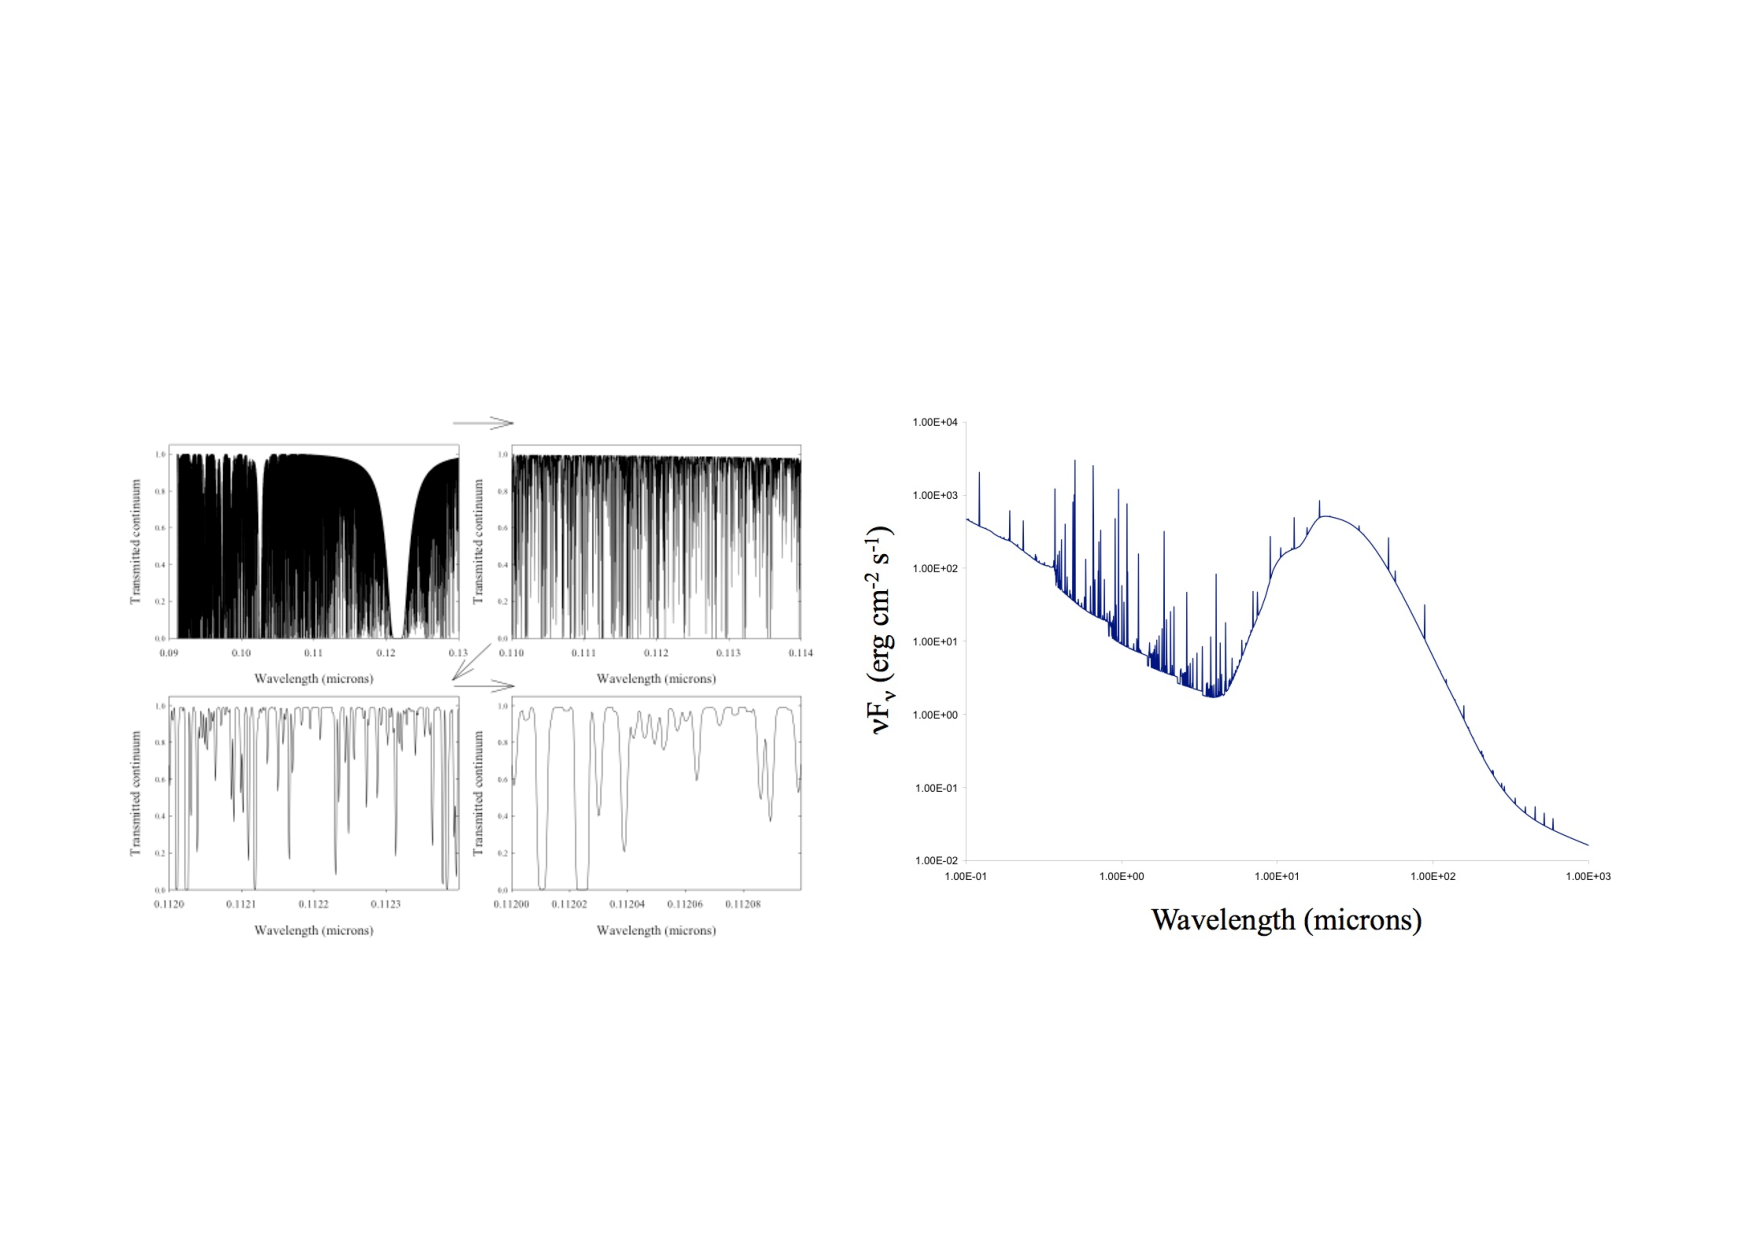
\includegraphics[scale=0.6]{CoarseFineContinua}
\caption[Orion Spectrum]{\label{fig:CoarseFineContinua}The spectrum of the Orion H~II region / PDR
at a point near the H$^0$ - \htwo\ transition.
The left panel shows the fine continuum and is taken from Figure 20 of \citet{Shaw2005}
It shows the extinction of the stellar SED by absorption lines formed in the gas.
The right panel shows the coarse continuum for a cloud stopping at this point and
mainly shows the extinguished stellar SEC also with dust and gas emission.}
\end{figure}

The spectral resolving power is defined as $E/\delta E$, where $E$ is the
photon energy and $\delta E$ the width of the resolution element.  The number
of energy bins needed to store the radiation field is proportional to the
resolving power.  The number of bins is a major pace setter for the code since it
must continuously reevaluate various integrals over the radiation field.
The resolving power of the
coarse continuum is defined in the file \cdFilename{continuum\_mesh.ini}
in the data directory.
This file is designed to be changed by the user and can be
changed to much higher resolving power if need be.  This is all described in
the Chapter \cdSectionTitle{The Continuum Mesh} in Part 2 of this document.
The resolution of the coarse continuum for a particular model can also be changed with the 
\cdCommand{set continuum resolution} command described on 
page \pageref{sec:CommandSetContinuumOptions}.
If you change the continuum resolution you will need to recompile
the stellar continuua and grain opacities so that their energy grid
agrees with that used by the code.

The resolving power of the fine continuum is established at the start of a calculation.
It needs to resolve lines, so the resolution depends on the lowest possible kinetic temperature
and any turbulence that may be present.
The \cdCommand{set fine continuum} command described on 
page \pageref{sec:CommandSetFineContinuum}
can also adjust this resolution.

\section{Defining a single component of the incident radiation field}

Two quantities, the \emph{shape} and \emph{intensity},
specify a single component of the incident radiation field.
The shape gives the form of the spectral energy distribution
but not its intensity.
The intensity can be specified as either the energy striking
the illuminated face of the cloud, referred to as
the intensity case, or both the source luminosity and the
distance separating the source and the cloud.  
The latter is referred to as the luminosity case.
The shape and intensity are specified independently
in most cases, although some commands specify both 
(the command specifying
the cosmic microwave background is an example of the latter).

In much of the following discussion we will refer to both
luminosity and intensity commands as simply intensity commands.
The distinction between the luminosity and intensity cases
is discussed further on page \pageref{sec:IntensityLuminosityCases}.

\section{Combining several radiation fields}

\subsection{The sum of several radiation fields}

It is possible to combine up to 100 incident radiation fields.\footnote{
Restrictions on the number of tables that could be entered existed
in \Cloudy\ versions 73 and before, but have been lifted. Restrictions on
which types of continua could be combined existed in \Cloudy\ versions 67
and before, but have been lifted.}   \Cloudy\ will stop if
more than 100 continua are entered.
This limit is set by the variable \cdVariable{LIMSPC}
that occurs in one of the included header files.

When more than one radiation field is entered the series of luminosity and
shape commands must be in the same order (i.e., map one to one).  There
must always be exactly the same number of luminosity and shape
specifications; \Cloudy\ will stop if there are not.

As an example, the following would be a rough approximation of an
accretion disk and boundary layer around a white dwarf:
\begin{verbatim}
# this is the black body associated with the boundary layer
# this is a shape command
black body, temperature =5e5 K
# this gives its total luminosity 
luminosity (total) 37.3
# the following shape is a rising power law, 
# a simple approximation to the disk 
power law, slope = 1.333, cutoff = 0.6 Ryd
# the total luminosity of this power law component
luminosity (total) 37.2
\end{verbatim}
The $5\times 10^5 \K$ blackbody has a total luminosity of
$10^{37.3} \ergps$ while
the power-law has a total luminosity of
$10^{37.2} \ergps $.

\subsection{Keeping shape and intensity commands together}

\noindent It is not absolutely necessary to keep
the ordered pairs of shape and
intensity commands together but this is a good practice
since some commands
(those given in Table \ref{tab:ShapeIntensityCommands})
specify \emph{both} the shape \emph{and} intensity of the incident
radiation field.
Problems arise if one of the commands giving both shape and intensity is
entered between another pair of shape and intensity commands.
For instance, the following will produce unintended results:
\begin{verbatim}
black body, temp = 5e5 K
CMB, z=2
luminosity (total) 37
\end{verbatim}
because the \cdCommand{CMB} command enters both the
shape and intensity of the cosmic microwave background.
In this example it comes after the \cdCommand{blackbody} command
specifies a shape, but before the \cdCommand{luminosity} command
specifies the luminosity of the blackbody.
As a result the intensity implicitly entered by the
\cdCommand{CMB}
command will apply to the hot blackbody rather than the cosmic
microwave background and the \cdCommand{luminosity} command will
then incorrectly set
the intensity of the cosmic background blackbody shape.
This problem cannot
occur if the shape and intensity commands are always kept together as in
the previous example.  The code should produce a warning if shape and
luminosity commands are mixed together with a command that enters both.

\begin{center}
\begin{table}
\centering
\caption{\label{tab:ShapeIntensityCommands}
Commands specifying both shape \emph{and} intensity}
\label{table:3}
\begin{tabular}{c}
\hline
background\\
 blackbody, energy density\\
blackbody, LTE\\
blackbody,
luminosity\\
blackbody, radius\\
CMB\\
table Draine\\
table HM96, HM05, HM12\\
table ISM\\
table read scale\\
\hline
\end{tabular}
\end{table}
\end{center}

\section{Check the incident radiation field!}

It is important to check that the incident radiation field
has been entered correctly.
First set up the commands to do a simulation and include the \cdCommand{save continuum} command
(described on page \pageref{sec:CommandSaveContinuum}).
Do the simulation and examine the
file produced by the \cdCommand{save continuum} command.
The first column gives the
photon energy and the second gives the incident radiation field
(as $\nu J_{\nu}$, erg cm$^{-2}$~s$^{-1}$)
at the illuminated face of the cloud.
Plot this radiation field and check that it is correct.

   
\chapter{INCIDENT RADIATION FIELD LUMINOSITY}
\label{sec:IncidentRadiationFieldLuminosity}
% !TEX root = hazy1.tex
\section{Overview}

All commands setting the intensity or luminosity of the
incident radiation field are
defined in this Chapter.

\section{Intensity and luminosity cases}
The brightness of the incident radiation field can be specified
as either an intensity, the energy per unit area of cloud,
or as a luminosity, the power emitted by the central
source of radiation into $4 \pi \sr$.
The \cdTerm{intensity case} and \cdTerm{luminosity case}
are described on page \pageref{sec:IntensityLuminosityCases}.
Each of the following commands is listed as an intensity or
luminosity command.
This distinction is important because the inner radius of the
cloud must also be specified in the luminosity case.

\section{The range option}

Many of the intensity/luminosity commands specify the number of photons
or integrated energy \emph{in hydrogen-ionizing radiation}
$(1 \Ryd \le h\nu \le$ \egamry ).
Other
energy intervals can be specified with the \cdCommand{range} option, an optional keyword
that can appear on most intensity / luminosity commands.

When the keyword \cdCommand{range} appears there are an
additional two parameters,
the low- and high-energy limits to the energy range in Rydbergs.
These
appear as the second and third numbers on the line
(the first number gives
the intensity or luminosity).
The position of the keyword \cdCommand{range} on the
command line does not matter but the order of the numbers on the line does
matter.
If both range parameters are omitted then the low
(\emm ) and high (\egamry )
energy limit of the incident radiation field will be
substituted.  If both energies are specified then the
second number must be larger than the first.
If only
one parameter appears then only the lower limit of the range
will be changed
and the high-energy limit will be left at its default of
\egamry .
If the first optional number is negative or
the keyword \cdCommand{log} appears then
\emph{both} of the extra numbers are interpreted as logs.
If you want to set the lower limit of the range to the low
energy limit \emm\ of the incident radiation field, but want
to supply your own upper limit, you can enter 0 followed by
the upper limit if you use linear numbers, or $-10$ followed by
the upper limit if you use log numbers ($-10$ is actually any
number $\leq$ log(\emm)).

If \cdCommand{range total}, or simply \cdCommand{range} or \cdCommand{total},
appears with no parameters then the
full energy range considered by the program,
\emm\ to
\egamry , will be used.
In this case the number is the total integrated (bolometric) intensity
or luminosity.

The following shows examples of the range option for the
\cdCommand{luminosity} command.
By default the \cdCommand{luminosity} command has a single parameter,
the log of the luminosity [erg s$^{-1}$] in hydrogen-ionizing
radiation ($1 \Ryd \le  h\nu <$ \egamry ).
The ``;'' symbol is used to terminate the line in one
case.
\begin{verbatim}
# this will use the default range, only ionizing radiation
luminosity 38 #the log of the luminosity in erg s^-1

# either will be the total luminosity
luminosity total 38
luminosity 33.4 range
luminosity 33.4 range total

# this will be the luminosity in visible light
luminosity 37.8 range .15 to .23 Ryd

# the luminosity in radiation more energetic than 0.1 Ryd
luminosity 38.1 range -1

# this will be the luminosity in non-ionizing radiation
luminosity 39.8 range 0 1
\end{verbatim}

\section{Absolute [visual, bolometric] magnitude -2.3}

It is possible to specify the integrated or monochromatic luminosity
in ``magnitudes,'' a quaint unit of historical interest.
One of the keywords
\cdCommand{bolometric} or \cdCommand{visual} must also appear.
The absolute bolometric magnitude
$M_{bol}$ is related to the total luminosity by (\citealp{Allen1976}, page 197)
\begin{equation}
L_{total}  = 3.826 \times 10^{33}  \times 10^{\left( {4.75 - M_{bol} }
\right)/2.5}\,
 [\ergps].
\end{equation}
The absolute visual magnitude $M_V$ is approximately related to the
monochromatic luminosity per octave at 5550 \AA\
by (\citealp{Allen1976}, page 197)
\begin{equation}
\nu \,L_\nu  \left( 5500\mathrm{\AA}\right) \approx 2.44 \times 10^{35}
\times 10^{ - M_V /2.5}\,
[\ergps].
\end{equation}
The conversion between monochromatic luminosity per octave $\nu L_{\nu}$ and absolute
visual magnitude $M_V$ is approximate,
with typical errors of roughly a percent.
This is because \Cloudy\ assumes that the V filter has an
isophotal wavelength of 5550\AA\ and does not actually integrate
over the incident radiation field using
a $V$-filter transmission function.

This is a luminosity command.

\section{Energy density 5e4 K [linear]}

This specifies the energy density [K] of the incident radiation field.
The number is the equivalent energy-density temperature, defined as
$T_u  = \left( {u/a} \right)^{1/4} \K$
where $u$ is the total energy density in all radiation
[erg cm$^{-3}$] and $a$ is the Stefan radiation-density constant.
The number is interpreted as the log of the temperature if it is less than or equal to 10
or the keyword \cdCommand{log} is present,
and as a linear number otherwise.
The optional keyword \cdCommand{linear} forces the
number to always be interpreted as a linear temperature.

This is an intensity command.

\section{f(nu) = -12.456 [at .1824 Ryd]}

This specifies the monochromatic intensity at an arbitrary energy.  The
first number is the log of the monochromatic mean intensity at the
illuminated face of the cloud,
$4\pi J_\nu$ (with units erg
s$^{-1}\mathrm{Hz}^{-1} \mathrm{cm}^{-2})$, where
$J_{\nu}$ is the mean intensity of the incident radiation field
per unit solid angle.

The optional second number is the frequency in Rydbergs where
$4\pi J_\nu$ is specified.
The default is 1 Ryd.
In the example above the incident radiation field is
specified at 0.1824 Ryd = 5000\AA.
The frequency can be any within the energy
band considered by the code,
presently \emm\ to \egamry .
If the energy is less than or equal to zero then it is interpreted as the
log of the energy in Rydbergs, and as the linear energy itself if positive.

This is an intensity command.

\section{Intensity 8.3 [range, linear]}
\label{sec:IntensityCommand}

This specifies the integrated mean intensity,
$4\pi J$, [erg cm$^{-2}\mathrm{s}^{-1}$] at the
illuminated face of the cloud
\begin{equation}
4\pi J= \int_{v1}^{v2}4\pi J_v \; dv \,[\ergpscmps] .
\end{equation}
This is the per unit area equivalent of the \cdCommand{luminosity}
command.
The number is the log of the intensity unless the optional
keyword \cdCommand{linear} appears.
Unlike the majority of the commands, the first
five characters of the line must be entered.

The default range is over hydrogen-ionizing energies
(1 Ryd  $\le hv\le$ \egamry ).
The range option can be used to adjust
the values of $v_1$ and $v_2$.

Some of the interstellar medium and photo-dissociation region (PDR)
literature specifies the incident radiation field in units of the
\citet{Habing1968} field (see, for instance, \citealp{Tielens1985a},
\citealp{Tielens1985b}).
This
radiation field has an integrated intensity of
$1.6\times 10^{-3} \ergpscmps$ between
the limits of 6 and 13.6 eV (\citealp{Tielens1985a}; \citealp{Hollenbach1991}).
This integrated intensity is sometimes referred
to as $Go$.
The incident radiation field described by Tielens and Hollenbach,
but with an
intensity of 1 $Go$, could be generated with the commands:
\begin{verbatim}
# a B star with an intensity roughly the Habing 1968 radiation field
blackbody 3e4 K
intensity -2.8, range 0.44 to 1 Ryd
# remove all H-ionizing radiation
extinguish by 24, leakage = 0
\end{verbatim}
This set of commands sets the shape of the Balmer continuum to
that of a hot blackbody, sets the intensity to the Habing value,
and then extinguishes
all hydrogen-ionizing radiation,
as is assumed in the PDR literature.

This is an intensity command.

\section{ionization parameter $= -1.984$}

The ionization parameter is the dimensionless ratio of hydrogen-ionizing
photon to total-hydrogen densities.  It is defined as
\begin{equation}
U \equiv \frac{{Q\left( {\mathrm{H}} \right)}}{{4{\kern 1pt} \pi \,r_{\mathrm{o}}^2
\,n\left( {\mathrm{H}} \right)\,c}} \equiv \frac{{\Phi \left( {\mathrm{H}}
\right)}}{{n\left( {\mathrm{H}} \right)\,c}}%(6)
\end{equation}
(AGN3, equation 14.7, page 357).
Here $r_o$ is the separation [cm] between
the center of the source of ionizing radiation and the illuminated face
of the cloud, $n$(H) [cm$^{-3}$] is the
total\footnote{Before version 65 of the code the
electron density was used rather
than the hydrogen density.
Before version 75 $n$(H) was the atomic/ionic
hydrogen density, and did not include molecules.}
hydrogen density (ionized, neutral,
and molecular), $c$ is the speed of light,
$Q(\mathrm{H})$ [s$^{-1}$] is the number of
hydrogen-ionizing photons emitted by the central object,
and $\Phi(\mathrm{H})$
[cm$^{-2}\, \mathrm{s}^{-1}$] is the surface flux of ionizing photons.
The number is interpreted
as the log of $U$ unless the keyword \cdCommand{linear} appears.
The ionization parameter
is a useful quantity in plane-parallel, low-density, constant-density,
models, because of homology relations between models with different photon
and gas densities but the same ionization parameter (see \citealp{Davidson1977}).

This is an intensity command.

\section{L(nu) = 24.456 [at .1824 Ryd]}

This sets the monochromatic luminosity
$L_{\nu}$ [erg s$^{-1} \mathrm{Hz}^{-1}$] of the central object.
The first number is the log of the luminosity.
The optional
second number is the frequency in Rydbergs where $L_{\nu}$ is specified.  The default is 1 Ryd.
In the example above the incident radiation field is specified at
$0.1824 \Ryd = 5000 $\AA.
The frequency can be any within the energy band considered
by the code, presently \emm\ to \egamry .  If the energy is
less than or equal to zero then it is interpreted as the log of the energy
in Rydbergs, and the linear energy itself if positive.

This is a luminosity command.
\label{sec:LuminosityCommand}

\section{luminosity 38.3 [solar, total, range, linear]}

The number is the log of the integrated luminosity\footnote{Before version 83 of the code, the luminosity command was used to
enter both luminosity and intensity.  The code decided between the two by
checking on the resulting ionization parameter.  There are now separate
intensity and luminosity commands.} emitted by the central
object into $4\pi$~sr,
\begin{equation}
L = 4 \pi R_{star}^2 \int_{\nu _1 }^{\nu _2 } {\pi F_\nu
\, d\nu } [\ergps ].% (7)
\end{equation}
The default range is over hydrogen-ionizing energies ($1\mathrm{ Ryd} \le
h\nu\le$ \egamry ).  The \cdCommand{range} option can be used to adjust
the values of $\nu_1$ and $\nu_2$.

If the optional keyword \cdCommand{solar} appears
the number is the log of the \emph{total} luminosity relative to the sun. 
It is the log of the total luminosity if the keyword \cdCommand{total} appears.
If the
\cdCommand{linear} keyword is also used then the quantity will be the luminosity itself
and not the log.
The \cdCommand{range} option cannot be used if the luminosity is the
total luminosity or it is specified in solar units.
It will be ignored
if it appears.

The following are examples of the luminosity command.
\begin{verbatim}
# log of luminosity (erg/s) in ionizing radiation
luminosity 36

# roughly the Eddington limit for one solar mass
luminosity total 38

# both are a total luminosity 1000 times solar since
# solar specifies the total luminosity relative to the sun
luminosity solar 3
luminosity linear solar 1000

# this will be the luminosity in visible light
luminosity 37.8 range .15 to .23 Ryd
\end{verbatim}
This is a luminosity command.

\section{nuF(nu) = 13.456 [at .1824 Ryd]}

This command specifies the log of the monochromatic mean intensity
per octave $4\pi \nu J_\nu  $ [erg s$^{-1}$ cm$^{-2}$]
at the illuminated face of the cloud.
Here $J_{\nu}$ is the
mean intensity of the incident radiation field.

The optional second number is the energy (Ryd) where
$4\pi \,\nu J_\nu  $ is specified.
The default is 1 Ryd.  In the example above the incident radiation field
is specified at $0.1824 \Ryd = 5000\AA$.
The energy can be any within the
energy band considered by the code,
presently \emm\ to \egamry .
If the energy is less than or equal to zero it is interpreted as the
log of the energy in Rydbergs.  It is the linear energy if it is positive.

This is an intensity command.

\section{nuL(nu) = 43.456 [at .1824 Ryd]}

This command specifies the monochromatic luminosity per octave
$\nu L_\nu$ [erg s$^{-1}$].
The first number is the log of the luminosity radiated by the central
object into $4\pi$~sr.  It can be expressed at an arbitrary photon
energy but the default is 1 Ryd.

The optional second number is the energy (Ryd) where $L_\nu$ is
specified.
In the example above the incident radiation field is specified
at 0.1824 Ryd = 5000\AA.
The frequency can be any within the energy band considered by
the code, presently \emm\ to \egamry .  If the energy is less
than or equal to zero, it is interpreted as the log of the energy in
Rydbergs, and the linear energy if positive.

This is a luminosity command.

\section{phi(H) = 12.867 [range\dots]}

This command specifies the log of $\Phi(\mathrm{H})$,
the surface flux of
hydrogen-ionizing photons [cm$^{-2}\ \mathrm{s}^{-1}$]
striking the illuminated face of the cloud.
It is defined as
\begin{equation}
\Phi \left( {\mathrm{H}} \right) \equiv \frac{{Q\left( {\mathrm{H}} \right)}}{{4\,\pi
\;r_{\mathrm{o}}^{\mathrm{2}} }} \equiv \frac{{R_{star}^2 }}{{r_{\mathrm{o}}^2
}}\;\int_{\nu _1 }^{\nu _2 } {\frac{{\pi \,F_\nu  }}{{h\,\nu }}\;d\nu }
 [\mathrm{cm}^{-2}\ \mathrm{s}{^{-1}]}
\end{equation}
and is proportional to the optical depth in excited lines,
such as the Balmer lines (\citealp{FerlandNetzerShields1979}; AGN3).
The range option can be
used to change the default energy range,
given by the values of $\nu_{1}$ and $\nu_{2}$.

This is an intensity command.

\section{Q(H) = 56.789 [range\dots]}

This is the log of the total number of ionizing photons emitted by the
central object [s$^{-1}$]
\begin{equation}
Q\left( {\mathrm{H}} \right) = 4\,\pi \;R_{star}^2 \;\int_{\nu _1 }^{\nu _2
} {\frac{{\pi \,F_\nu  }}{{h\,\nu }}\;d{\kern 1pt} \nu } . %(9)
\end{equation}
The default energy range is 1 Ryd to \egamry\
and the \cdCommand{range} option
can be used to change the energy bounds $\nu_1$ and $\nu_2$.
The photon flux (the
number of photons per unit area of cloud surface) can be specified with
the \cdCommand{phi(H)} command\footnote{Before version 83
of the code the \cdCommand{phi(H)} and \cdCommand{Q(H)} commands were the
same.
The code decided which was specified by checking the order of
magnitude of the resulting ionization parameter.
These are now two different commands.}.

This is a luminosity command.

\section{ratio -3.4 0.3645 Ryd to 147 Ryd [alphaox, log]}

This specifies the intensity of a second radiation field
(referred to as the current radiation field) relative to the
intensity of the previous
radiation field.
The ratio of the intensities
$4\pi J_\nu$ (erg cm$^{-2}\ \mathrm{s}^{-1}\ \mathrm{Hz}^{-1}$)
of the current to the previous radiation field is given
by the first number on the command line.
It is assumed to be the linear ratio unless it is
less than or equal to zero, in which case it is interpreted as a log.
If the keyword \cdCommand{log} appears then the
positive number is interpreted
as the log of the ratio.

The second parameter is the energy in Rydbergs where the previous
radiation field is evaluated and the optional third parameter
is the energy
where the current radiation field is evaluated.
If the second energy is not
entered then the same energy is used for both.
The following is an example
of using the \cdCommand{ratio} command to simulate the
spectral energy distribution of a typical quasar.
\begin{verbatim}
blackbody 5e4 K        # the big blue bump
ionization parameter -2 # its ionization parameter
table power law         #an alpha =-1 power law
# now set intensity of power law relative to bump at 1 Ryd
ratio 0.001 at 1 Ryd
\end{verbatim}
This command was introduced to provide a mechanism to specify the optical
to X-ray spectral index $\alpha_{ox}$.
This is defined here as in \citet{Zamorani1981}, except for a difference in sign convention.
Here $\alpha_{ox}$ is the spectral
index which would describe the continuum between 2 keV (147 Ryd) and
2500\AA\ (0.3645 Ryd) if the continuum could be described
as a single power-law, that~is,
\begin{equation}
\frac{{f_\nu  \left( {2\;{\mathrm{keV}}} \right)}}{{f_\nu  \left(
{2500\;{\mathrm{{\AA}}}} \right)}} = \left( {\frac{{\nu _{2\;{\mathrm{keV}}} }}{{\nu
_{2500\;{\mathrm{{\AA}}}} }}} \right)^{\alpha _{ox} }  = \,\;403.3^{\alpha _{ox}
} .% (10)
\end{equation}
The definition of $\alpha_{ox}$ used here is slightly different
from that of Zamorani et al. since implicit negative signs are
never used by \Cloudy.
Typical AGN have $\alpha_{ox}\sim  -1.4$.
If X-rays are not present then
$\alpha_{ox} = 0$.

The \cdCommand{ratio} command has an optional keyword,
\cdCommand{alphaox}, which allows $\alpha_{ox}$
to be specified directly.
If the keyword appears then only one parameter
is read, the value of $\alpha_{ox}$.
A generic AGN spectral energy distribution could be produced with
the following,
\begin{verbatim}
blackbody 5e4 K   # the big blue bump
ionization parameter -2
table power law    # an alpha =-1 power law
ratio alphaox -1.4 # set alpha_ox of the X-ray and UV continua
\end{verbatim}
Note that $\alpha_{ox}$ may (or may not) depend on the luminosity of the quasar,
as described by \citet{Avni1986}.
The solid line in their Figure 8 corresponds to
\begin{equation}
\alpha _{ox}  =  - 1.32 - 0.088 \times \log \left( {\frac{{L_o }}{{10^{28}
\,{\mathrm{erg}}\,{\mathrm{s}}^{ - {\mathrm{1}}} \,{\mathrm{Hz}}^{ - {\mathrm{1}}} }}} \right)% (11)
\end{equation}
where they define $L_o$ as the monochromatic optical luminosity
at 2500\AA\  in the source rest frame,
and we assume H$_0 = 50$ and q$_0 = 0$.
Other fits are given
by \citet{Worrall1987}:
\begin{equation}
\alpha _{ox}  =  - 1.11 - 0.111 \times \log \left( {\frac{{L_o }}{{10^{27}
\,{\mathrm{erg}}\,{\mathrm{s}}^{ - {\mathrm{1}}} \,{\mathrm{Hz}}^{ - {\mathrm{1}}} }}} \right)% (12)
\end{equation}
and by \citet{Wilkes1994}:
\begin{equation}
\alpha _{ox}  =  - 1.53 - 0.11 \times \log \left( {\frac{{L_o }}{{10^{30.5}
\,{\mathrm{erg}}\,{\mathrm{s}}^{ - {\mathrm{1}}} \,{\mathrm{Hz}}^{ - {\mathrm{1}}} }}} \right)
.% (13)
\end{equation}
However, \citet{LaFranca1995} find no dependence
of $\alpha_{ox}$ on luminosity.
\citet{Avni1995} find a complicated luminosity dependence.
Clearly this is an area of active research.

\emph{N.B.}  The net incident radiation field may have a
smaller than specified ratio of current
to total incident radiation field,
since the command specifies the ratio of the current
to the previous incident radiation fields,
not the ratio of current to total incident radiation field.
The ionization parameter will be slightly larger than
specified for the same reason.

In general, it is probably better to use the \cdCommand{AGN} command
rather than this command.

This is neither a luminosity nor intensity command---the units
of the previous radiation field carry over to this command.

\section{xi -0.1 }

\citet{Tarter1969, Krolik1981, 2001ApJS..133..221K} define an ionization parameter
$\xi$ given by
\begin{equation}
\xi  =  \left( {4\pi
} \right)^2 \int_{1R}^{1000R}  J_\nu  {\kern 1pt} d\nu /n\left( {\mathrm{H}}
\right)
= \frac{{F_{ion} }}{{n\left( {\mathrm{H}} \right)r^2 }}
\approx \frac{{L_{ion} }}{{n\left( {\mathrm{H}} \right)r^2 }}
 [\mathrm{erg\ cm\ s}^{-1}]
 \label{eqn:xi}
\end{equation}
where $n(\mathrm{H})$ is the hydrogen density at the illuminated face
of the cloud and $r$ is the source - cloud separation.
The number is the log of $\xi$.

The original \citet{Tarter1969} paper defined $\xi$ as the last term in equation \ref{eqn:xi}, 
with $L_{ion}$ defined as including all ionizing radiation.  
\Cloudy\ used this definition, integrating over all ionizing photon energies,
through version C13.03.  

The 1 - 1000 Ryd  energy range first appears in \citet{Krolik1981}, 
in the discussion above eqn 2.2a, 
but they introduce a new variable, $F_{ion}$, for the luminosity over this range.
The XSTAR code \citep{2001ApJS..133..221K} defines  $\xi$ over 1 - 1000 Ryd.

Beginning with C13.04 the XSTAR definition is used for $\xi$,
for compatibility with that code.
That is, we now integrate over 1 - 1000 Ryd.
The middle and right terms in equation \ref{eqn:xi} are not equal for a hard SED.

You can easily define your own energy intervals by using the \cdCommand{luminosity},
page \pageref{sec:LuminosityCommand},
or \cdCommand{intensity}, page \pageref{sec:IntensityCommand}, commands to specify $L$ or $4\pi J$.
They both accept the \cdCommand{range} option to change the limits in equation \ref{eqn:xi}.

   
\chapter{INCIDENT RADIATION FIELD SHAPE}
% !TEX root = hazy1.tex
\label{sec:IncidentContinuumShape}

\section{Overview}

The spectral energy distribution (SED) of the
incident radiation field should be specified
between the energies of \emm\ ($\lambda \approx$ \emmcm )
and \egamrymev \ $\approx$ \egamry .
The low-energy region is important for Compton cooling,
photoionization
from excited states of the elements, free-free heating, H$^-$ heating,
and grain heating.
The high-energy portion is important for Auger and secondary
ionization, Compton heating, and pair production.
Energies greater than
100 MeV are not generally important since the Klein - Nishina
electron-scattering cross section is small.
\Cloudy\ will complain, but compute
the model if possible, if the
incident radiation field is not specified over the full energy range.
An intensity of zero will be assumed for missing portions of the
incident radiation field.

The \cdTerm{plasma frequency}, given by
\begin{equation}
\nu _{pl}  = \left( {\frac{{n_e q_e^2 }}{{\pi \,m_e }}} \right)^{1/2}  =
8.978 \times 10^3 \,n_e^{1/2} \;s^{ - 1}  = 2.729 \times 10^{ - 12}
\;n_e^{1/2} \;{\mathrm{Ryd}},% (15)
\end{equation}
will move into the energy range considered by the code if the electron
density is higher than $\sim 10^7 \mathrm{cm}^{-3}$.
The incident radiation field below the
plasma frequency is totally reflected and does not enter the slab.
The code will generate a comment if the plasma frequency occurs within
the energy grid.

\emph{It is important to plot the incident radiation
field using the output of the
\cdCommand{save continuum} command to make sure the SED has the expected shape.}
It is easy to make a mistake in converting between $f_\nu$, $f_\lambda$,
$\nu f_\nu$, and $\lambda f_\lambda$ when deriving the SED.
The \cdCommand{save continuum} command will report the SED in 
$\nu f_\nu$ or $\lambda f_\lambda$ units (the two are equivalent).

\subsection{Isotropic and beamed continua}
Most radiation fields are assumed to strike the cloud as a
single-directional beam.
The beam is assumed to enter the slab normal to
the surface, unless this is changed with the
\cdCommand{illumination angle} command.
Other commands, including
\cdCommand{background}, \cdCommand{blackbody STE}, \cdCommand{CMB},
\cdCommand{table HM96}, \cdCommand{table HM05},
\cdCommand{table HM12}, \cdCommand{table KS19}, and \cdCommand{table ISM},
generate continua that are isotropic.
Each shape command will indicate whether the SED is isotropic or beamed.

Many spectrometers will automatically remove isotropic emission while
conducting an observation.  Some isotropic continua, especially the CMB at
radio wavelengths, will dominate over local emission.
The radiation field used in the calculation is reported by default, although
there are two commands that will suppress isotropic emission.
The \cdCommand{save continuum} command,
section \ref{sec:CommandSaveContinuum}, includes a \cdCommand{no isotropic}
option, described in section \ref{sec:save_cont_no_isotropic_option}, to suppress
isotropic emission in that file.
The \cdCommand{no isotropic continua report} command described
in section \ref{sec:no_isotropic_continua} will suppress
Isotropic emission in both \cdCommand{save continuum}  files
and the continuum bands described in
Section~\ref{Hazy2-sec:Radiation-field-integrated-over-wavelengths}
\cdSectionTitle{\refname{Hazy2-sec:Radiation-field-integrated-over-wavelengths}}.


\section{AGN T =1.5e5 k, a(ox) = -1.4, a(uv)=-0.5 a(x)=-1}

This produces a multi-component continuum similar to that observed in
typical Active Galactic Nucleus (AGN).
An example is shown in Figure \ref{fig:agncon}.
The ``Big Bump'' component, peaking at $\approx 1$ Ryd,
is a rising power law with
a high-energy exponential cutoff.
It is parameterized by the temperature
of the bump, the first argument on the command line.
It is interpreted
as the log of the temperature if it is less than or equal to 10 and the
linear temperature otherwise.
The temperature of the bump can by optimized by using the \cdCommand{vary} keyword.
The second parameter is the X-ray to UV ratio
$\alpha_{ox}$.
Note that there
is no implicit negative sign in this exponent; typical AGN have
$\alpha_{ox} \sim
-1.4$, (\citealp{Zamorani1981}).
The third (optional) argument is the
low-energy slope of the Big Bump continuum,
with the default $\alpha_{uv} = -0.5$
(\citealp{Elvis1994}; \citealp{Francis1993}).
The last argument is the slope of the
X-ray component with the default $\alpha_x = -1$.
Optional parameters can be omitted
from right to left.

\begin{figure}
\centering
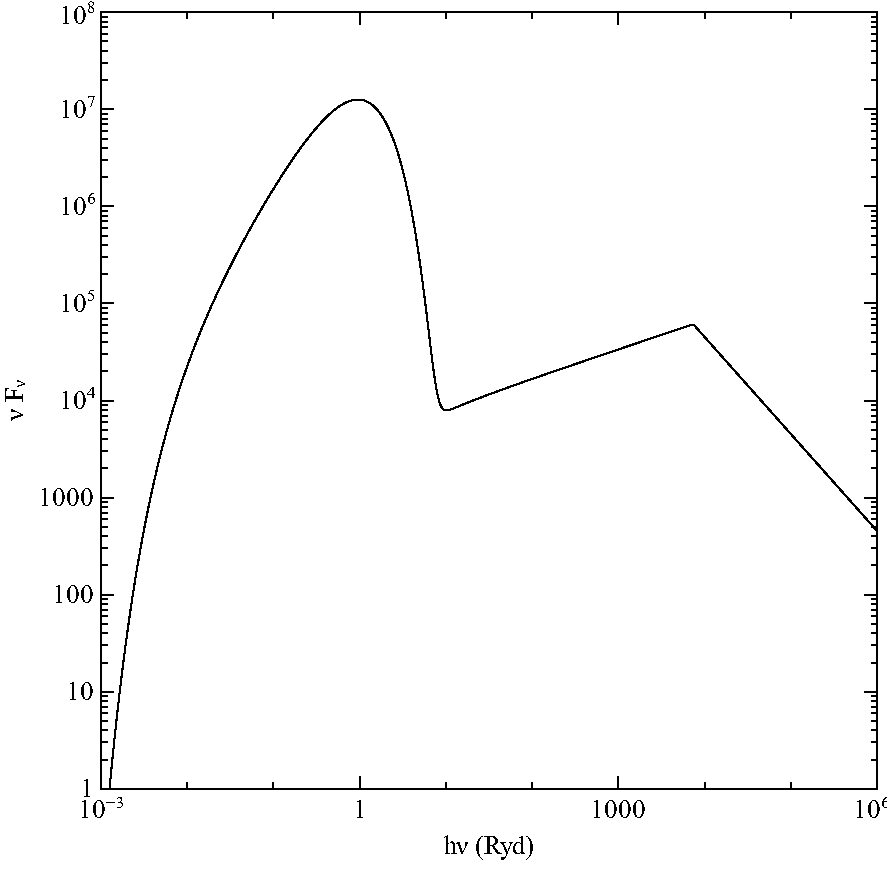
\includegraphics[scale=0.75]{AGNCON}
\caption[AGN SED]{\label{fig:agncon}The continuum produced by the
\cdCommand{AGN} continuum command.
The Big Bump peaks at $\approx1$~Ryd,
while the X-ray power law dominates at high energies.
The two components are normalized by the second parameter, the value of
$\alpha_{ox}$.}
\end{figure}

The full continuum is the sum of two components,
as in equation \ref{eqn:agncon}:

\begin{equation}
\label{eqn:agncon}
f_\nu   = \nu ^{\alpha _{uv} } \exp \left( { - h\nu /kT_{BB} } \right)\exp
\left( { - kT_{IR} /h\nu } \right)\; + a\nu ^{\alpha _x }. % (16)
\end{equation}
The coefficient $a$ is adjusted to produce the
correct $\alpha_{ox}$ for the case where
the Big Bump does not contribute to the emission at 2~keV.
If the bump
is very hot then it may contribute to the X-rays as well and
the resulting
continuum will have a more negative $\alpha_{ox}$ than specified.
The X-ray power
law is only added for energies greater than 0.1 Ryd to prevent
it from
extending into the infrared, where a power law of this slope
would produce
\emph{very} strong free-free heating.
The Big Bump component is assumed to have
an infrared exponential cutoff at $kT_{IR} = 0.01 \mathrm{Ryd}$.

The last term in equation \ref{eqn:agncon} is not extrapolated
below 1.36 eV or above 100 keV.
Below 1.36 eV the last term is simply set to zero (the bump
dominates for these energies).
Above 100 keV the continuum is assumed to
fall off as $v^{-2}$.

The exponential cutoff in the low-energy end of the Big Bump will cause
the incident continuum to have zero intensity at very long wavelengths.
The code will complain since a zero incident continuum is unphysical, but
the model will be computed.
You can prevent the continuum from going to
zero by including the cosmic background with the
\cdCommand{background} command or with the \cdCommand{CMB} command.

We used this command to generate the continuum used in a large atlas
of BLR line intensities (\citealp{KoristaBaldwin1997}).
The specific parameters
needed to reproduce that continuum are
\cdCommand{AGN 6.00 -1.40 -0.50 -1.0}.  Only
Kirk Korista can remember all these numbers and the parameters were not
explicitly given in the original paper in the format used by the code.
The \cdCommand{kirk} option on the \cdCommand{AGN} command will
generate that continuum.
It is fairly
similar to the \citet{Mathews1987} continuum but there is
much greater
flexibility in changing its details.

\section{Background, z=1.825, [f=100; no CMB]}

This specifies a radiation field shape and intensity
chosen to mimic the cosmic
radio to X-ray background (\citealp{Ostriker1983}, \citealp{Ikeuchi1986}, and \citealp{Vedel1994}).
Their ultraviolet
continuum shape is an $\alpha = -1$ power-law, with a mean intensity
$J_\nu$ at 912\AA\ given~by
\begin{equation}
4\,\pi \;J_\nu  \left( {912{\mathrm{{\AA}}}} \right) = 4\,\pi \, \times 10^{
- 21} \left( {\frac{{1 + z}}{{3.5}}} \right)^4 \quad f [\mathrm{erg\, Hz}^{-1}
\mathrm{cm}^{-2} \, \mathrm{s}^{-1}]
\end{equation}
where $z$ is the redshift and $f$ an optional scale factor entered as
the second parameter.
Its default value is $f = 1$, and $z = 0$ (i.e., now) is assumed
if no redshift is entered.
Judging from \citet{Bechtold1987}, \citet{Bajtlik1988}, and \citet{Vedel1994},
$f$ is confidently known to be within an order of magnitude of unity.

This command specifies \emph{both} the shape and intensity
of the incident radiation field.
It is important that any previously occurring ordered pairs of shape and
intensity commands be complete before this command is given.

Cosmic microwave background radiation is included in the generated
background.
This radiation field is assumed to be a blackbody radiation
field, in strict thermodynamic equilibrium, with temperature given~by
\begin{equation}
T_{CMB}  = T_o \left( {1 + z} \right)\; [\mathrm{K}]% (18)
\end{equation}
where the redshift dependence is from \citet{Peebles1971} and the present
temperature of the background is assumed to be $T_o = 2.725 \pm 0.002$K
(\citealp{Mather1999}; \citealp{Wilkinson1987}).
This background can be an important source
of Compton cooling for low-density clouds.
If the optional keyword
\cdCommand{no CMB}
appears on the line then the CMB background will not be included.
The CMB can be specified independently with
the \cdCommand{CMB} command.

The \cdCommand{table HM96} command uses a more sophisticated
form of the energetic continuum, but only at a redshift of $z = 2$.
The \cdCommand{table HM05} and \cdCommand{table HM12}
commands work at any redshift.

This command does not add the cosmic-ray background.
This should be
included if the simulation is to extend into molecular gas and is done
separately with the \cdCommand{cosmic ray} command.

This radiation field is assumed to be isotropic rather than beamed.

\section{Blackbody t=e5 K [linear, log, luminosity]}

The continuum will be a blackbody with temperature (K) given by the
number.
The temperature may be entered directly or as a log.
The number
is assumed to be a log if it is less than or equal to 10 and linear if
greater than 10.
The keywords \cdCommand{log} and \cdCommand{linear} will override
this default
and force the interpretation of the numbers to be either a log or linear.
Embedded commas can improve readability, such~as
\begin{verbatim}
black body, Temp = 1e6 K
\end{verbatim}
which is equivalent to
\begin{verbatim}
black 1000000
\end{verbatim}
or
\begin{verbatim}
black body t=6  .
\end{verbatim}

\subsection{Blackbody, t = 1e5 K, disk = 1e3 K}

This command produces a multi-color blackbody as if due to an accretion disk  with
inner and outer temperatures $T_{in}$ and $T_{out}$ as in \citet{Mitsuda1984}.  
The temperatures can be in either order; the code will automatically take the 
greater temperature as $T_{in}$.  

Neither the luminosity nor the intensity is set by this command.

\subsection{Peter Martin's blackbody luminosity options}

The luminosity of the black body can be specified with command-line
options added by P.G. Martin.
If the luminosity is specified
with any of these options then it must not also be specified with another
luminosity command for this radiation field.
The keywords that can appear
on the line are given in the following subsections.

\subsection{Blackbody 5, luminosity = 38.   }

If the keyword \cdCommand{luminosity} appears then the second number
is the log of
the \emph{total} luminosity (erg s$^{-1}$) of the black body, $4\pi \,R_{star}^2 \sigma T_{eff}^4 $
(this number is interpreted as a log even when the keyword \cdCommand{linear} appears on the line).
This example would be a 10$^5$~K planetary nebula nucleus at the Eddington
limit.

This is a luminosity command.

\subsection{Blackbody 5, radius = 10.  }

The log of the radius (in cm) of the blackbody $R_{star}$
is used to set the
total luminosity when the keyword \cdCommand{radius} appears
(this number is interpreted as a log even when the keyword \cdCommand{linear} appears on the line).
The total luminosity
is $4\pi \,R_{star}^2 \sigma T_{eff}^4 $.
This example is also typical of a planetary nebula nucleus.

This is a luminosity command.

\subsection{Blackbody 5e4 K, energy density = 500K.  }

The energy density of the blackbody radiation field, expressed as the
equivalent blackbody temperature $T_u$ in degrees Kelvin,
is used to set the
luminosity when the \cdCommand{energy density} keyword appears
anywhere on the line.
The energy-density temperature is defined from Stefan's law and the energy
density of the radiation field $u$~[erg cm$^{-3}$]:
\begin{equation}
T_u  \equiv \left( {\frac{u}{a}} \right)^{1/4}  [\mathrm{K}]% (19)
\end{equation}
where $a$ is the Stefan's radiation density constant.

Both temperatures are interpreted as logs if they are less than or equal
to 10 or the keyword \cdCommand{log} appears, and linear otherwise.  They will be interpreted as the linear
temperature rather than as a log if the keyword \cdCommand{linear} appears.  Note that
if the \cdCommand{linear} key is used then both temperatures are interpreted as linear.
Similarly, if the keyword \cdCommand{log} appears, both temperatures are interpreted as log.
Note also that the cosmic background radiation should also be included if
$T_u\le 2.725 (1+z) K$.
\Cloudy\ will complain, but compute the model, if the
energy density of the incident continuum corresponds to a temperature less
than the present energy-density temperature of the universe.

This is an intensity command.

\subsection{Blackbody, t = 5e4 K, STE  }

The keyword \cdCommand{STE}\footnote{The keyword was \cdCommand{LTE} before version 96 of the code.  It was changed
to \cdCommand{STE} to better reflect the fact that this condition corresponds to strict
thermodynamic equilibrium.
The code will continue to accept the \cdCommand{LTE} keyword
for the foreseeable future.}
(note that a space must appear before ``STE'') with no second number is
equivalent to the \cdCommand{energy density} option with $T_u$ set
to the color temperature
of the radiation field.
This is a quick way to check that ionization and
level populations go to strict thermodynamic equilibrium in the high
radiation-density limit.
The blackbody radiation field in the STE limit (but not the LTE limit!)
is assumed to be isotropic.

This is an intensity command.

\subsection{Blackbody, t = 1e5 K, dilution factor = -14}

Here the second parameter is the \cdTerm{dilution factor}
\cdTerm{W} defined as
\begin{equation}
W \equiv \frac{{J_\nu  }}{{B_\nu  }} \approx \frac{{\pi \,R_{star}^2
}}{{4\,\pi \;r_o^2 }},% (20)
\end{equation}
where $R_{star}$ is the radius of the star and $r_o$ is the separation
between the illuminated face of the cloud and the center of the star.
The approximation
on the RHS assumes that $R_{star} \ll r_o$.
The dilution factor can be entered
either directly or as a log. Any number $> 0$ will be interpreted as
linear, while any number $\leq 0$ will be interpreted as log.
The example above is a rough approximation of the radiation field within
a typical planetary nebula.

This is an intensity command.

\section{Bremsstrahlung, temp = 8}

The incident radiation field will be optically thin pure hydrogen bremsstrahlung
emission.
The shape is given~by
\begin{equation}
f_\nu   \propto \nu ^{ - 0.2} \,\exp \left( { - h\,\nu /kT} \right)\quad
[\mathrm{erg\, cm}^{-2} \mathrm{s}^{-1} \mathrm{Hz}^{-1}]. %(21)
\end{equation}
The argument is assumed to be the log of the temperature if it is
less than or equal to 10 or the keyword \cdCommand{log} is present, and linear otherwise.
The form of the continuum is
approximate since a simple power-law Gaunt factor is assumed and
the emission
from an optically thin gas with cosmic abundances is
actually characterized
by hundreds of overlapping emission lines (see, for example, \citealp{Kato1976}).

A more realistic radiation field could be produced by combining the
\cdCommand{coronal equilibrium} command with the
\cdCommand{save transmitted continuum} command
to generate a continuum which can be read in with
the \cdCommand{table read} command.

\section{CMB [redshift 1000]}

This command generates a blackbody radiation field in strict thermodynamic
equilibrium (that is, $T_{color} = T_u$, where $T_u$ is the energy-density
temperature).  The optional argument is the redshift $z$.
If it is not entered then $z = 0$ is assumed.
The temperature of the blackbody is given~by
\begin{equation}
T_{CMB}  = T_o \left( {1 + z} \right)\quad [\K]
\end{equation}
where the redshift dependence is from \citet{Peebles1971} and the present
temperature of the background is assumed to be $T_o = 2.725\pm 0.002$K
(\citealp{Mather1999}; \citealp{Wilkinson1987}).
This command specifies \emph{both} the shape and
intensity of the radiation field.
A starting radius of $10^{30}$~cm will be
assumed if no starting radius is specified.

\begin{shaded}
\subsection{\experimental The time option}
The keyword \cdCommand{time} will follow the time-dependent
recombination of an evolving universe.
This is now being developed by Ryan Porter and will be described in
Porter et al. (in preparation).

\subsection{\experimental The density option}
The keyword \cdCommand{density} will also specify the density at
the redshift.
\end{shaded}

This CMB radiation field is assumed to be isotropic rather than beamed.

\section{Extinguish column = 23, leak = 0.05, low  =4 Ryd}

This command will modify the shape of the
incident SED by extinction due
to photoelectric absorption by a cold neutral slab with column density given
by the first argument (entered as a log, cm$^{-2}$).
This extinction is applied \emph{after} the
radiation field has been fully generated and normalized
to the correct intensity.
The form of the extinction is a simple power-law fit to the
absorption curves calculated by \citet{Cruddace1974}.
The extinguished continuum $f_\nu'$ is
related to the initial continuum $f_\nu$~by
\begin{equation}
f'_\nu  \left( {\nu  \ge 1\,{\mathrm{Ryd}}} \right) = f_\nu  \left\{ {\eta
+ \left( {1 - \eta } \right)\exp \left( { - 6.22 \times 10^{ - 18} \,\nu
_{Ryd}^{ - 2.43} \;N\left( {\mathrm{H}} \right)} \right)} \right\}%  (23)
\end{equation}
where $N(\mathrm{H})$ is the total hydrogen column density (cm$^{-2}$), $\nu_{Ryd}$ is the frequency
in Rydbergs, and $\eta$ is the leakage.

The optional second number is the fractional leakage $\eta$ through the
absorber (see \citealp{FerlandMushotzky1982}).
This has a default value of
0, i.e., no leakage.
The leakage is interpreted as a log if it is negative
and linear otherwise.
If unexpected or unphysical results occur when the
\cdCommand{extinguish} command is given then it is likely that
nearly all ionizing
radiation has been attenuated.
A plot of the generated continuum (with
the \cdCommand{plot continuum} command) may prove interesting.  The code will stop if
the leakage is greater than 1.0 (100\%).

The optional third number is the lowest energy for the absorption to
occur.
The default is 1 Ryd and is appropriate if the absorption is mainly
due to atomic hydrogen.
The number is interpreted as linear Rydbergs if positive
and the log of the energy if less than or equal to zero.
The continuum
with energies below this cutoff energy will be unaffected by the absorption.
The non-ionizing $(h\nu < 1 \mathrm{Ryd})$ continuum can be extinguished by this command
but extrapolating the power law to these energies is nonsense.

The second two arguments are optional and may be omitted from right to
left.
The cutoff energy can only be changed if the leakage is specified.

The command acts by first generating the continuum shape with extinction
neglected.
The continuum is then normalized using any of the luminosity
or intensity commands
(i.e., \cdCommand{Q(H)}, \cdCommand{ionization parameter},
\cdCommand{luminosity}, etc.).
Only \emph{then} is the continuum extinguished.
The continuum that actually strikes
the illuminated face of the cloud \emph{does not}
have the intensity or luminosity
actually entered.  (These values would be correct were the extinction not
present.)  Physically, the luminosity of the central object is not changed
by the presence of an absorbing cloud along the line of sight.

This command should only be used as a quick test.  A more physical
way to extinguish the continuum would be to actually transmit it through
a model of the absorbing slab, save that continuum with the
\cdCommand{save transmitted continuum} command,
then use this filtered continuum with
the \cdCommand{table read} command.

\subsection{Extinguish optical depth 1.2, [options]}

If \cdCommand{optical depth} appears rather than
\cdCommand{column} then the first number is
the log of the Lyman continuum optical depth.
All other options are the same as the
\cdCommand{extinguish column} command.
\emph{N.B.} It really is the log of the optical depth,
not the linear optical depth.

\section{Interpolate [$\nu$(Ryd) or log $\nu$(Hz)], log(f$_\nu$)}

This command will be maintained for backwards compatibility,
but you should consider using the \cdCommand{table SED} command,
described on page \pageref{sec:CommandTableSED}, 
which does the same thing but with much greater flexibility.

The shape of the incident radiation field will be interpolated from
the table of points given
by this command.
The interpolation uses straight lines in log-log space.
There is no limit to the number of ordered pairs of points that can be entered.
Lines starting with the keyword \cdCommand{continue} can be used to continue entering values after
the initial \cdCommand{interpolate} line is filled.

Unlike the majority of the commands the first five characters of the
command must be entered.

The numbers are ordered pairs giving the energy and intensity.
The first number within each ordered pair of points is \emph{either}
the energy in Rydbergs
(linear \emph{or} as a log) or the log of the frequency (in Hertz).  \Cloudy\ assumes
that the log of the energy in Rydbergs was entered if the first number is
negative; that the log of the frequency (Hz) was entered
if the first number
is greater than 5; and linear Rydbergs otherwise.
Any of the three styles
can be chosen but it must be used consistently within the command.
If the
first energy is entered as zero then it is interpreted as the low-energy
limit of the code.
In this case the remaining energies will be interpreted
as linear Rydbergs if the second number is positive and the log of the
energies in Rydbergs if it is negative.
An energy of zero Rydbergs is not
allowed (except for the first),
and the energies must be in increasing order.

The second number in each ordered pair is the log of the relative flux
density per unit energy interval [$\log_{10}(J_\nu$)+constant] at that energy.
These
numbers are only used to set the shape of the continuum.
The constant in
the equation is set by one of the intensity or luminosity commands.

\emph{Heads up!}  The intensity is $J_\nu$ \emph{and not} $\nu J_\nu$.
You should check that this command has produced the SED you expect by creating
as plot by using the output from the \cdCommand{save incident continuum} command
described on page \pageref{sec:CommandSaveIncidentContinuum}.

The \cdCommand{interpolate} command can be freely mixed with other shape
commands and a total of up to 100 \cdCommand{interpolate} and \cdCommand{table} commands can be entered.\footnote{Limits to the
use of the
\cdCommand{interpolate} command existed in versions 73
and before, but have been lifted.}  Note that \cdCommand{table} and
\cdCommand{interpolate} are actually
two forms of the same command so that they store information in the same
arrays.
The total number of \cdCommand{table} and \cdCommand{interpolate} commands entered together cannot exceed 100.

As an example, the following approximates a metal-poor 4.5e4 K stellar
atmosphere.  The energies are entered in Rydbergs:
\begin{verbatim}
# following is 45000 K atmosphere from Shields and Searle
interpolate (0.00001 -11.106) (.58 -1.5792) (.99 -1.44) (1.01 -1.7018)
continue  1.8 -1.905) (1.81 -1.939) (2.57 -2.208) (2.59 -2.247) (3 -2.3994)
continue (3.02 -2.8193) (3.49 -2.9342) (3.51 -4.143) (3.99 -5.582)
continue (4.01 -6.3213) (6 -9.9) (10 -17.3) (20 -30) (1e7 -30)
q(h) = 52.778151
\end{verbatim}
Note that the continuum should be specified between
\emm\ and
\egamry\ even if the intensity is small.
If it is not fully specified
then a warning will be issued and a model computed with the unspecified
continuum set to zero.
As a further note, it is important that the continuum
be physically correct.
For instance, stellar model atmospheres predict
almost no X-ray emission while real OB stars \emph{are} X-ray sources
(although neglecting X-rays for these stars is generally a safe
approximation).
See page \pageref{sec:StarHighEnergyComponent} below
for a more detailed discussion.

\emph{This command sets the SED by specifying $f_\nu$ points.}
Other commands may use $\nu f_\nu$ or $\lambda f_\lambda$ units (the two are equivalent).
You should plot the final SED used by \Cloudy\ with the
\cdCommand{save continuum} command to make sure the SED has the expected shape.
It is easy to make a mistake in converting between $f_\nu$, $f_\lambda$,
$\nu f_\nu$, and $\lambda f_\lambda$ when deriving the SED.
The \cdCommand{save continuum} command will report the SED in 
$\nu f_\nu$ or $\lambda f_\lambda$ units.

\section{Laser, frequency = 3.5 Ryd [rel width 0.02]}

The intensity of the radiation field will be very small
except within $\pm5$\% of the specified energy where it will be very large. The energy is specified
in Rydbergs and it is interpreted as a log if it is negative.
This is
provided as a way to check on the computation of the photoionization rate
integrals.

The optional second number changes the relative width of the laser.
The relative width is the ratio $dE/E$ where $dE$ is
the half width of the laser.
The laser will only be active within $\pm  dE$ of $E$.
The code would return
an error condition if $dE$ is so small that the laser does not
happen to be
within $\pm  dE$ of $E$ as evaluated by the code's energy mesh.
The fractional
width probably should not be made smaller than roughly 0.01 but the code
does not protect against too small a value of~$dE$.

Another way to make a laser is to save out a transmitted radiation field using the \cdCommand{save transmitted continuum} command,
edit this file, and, by hand, increase the intensity of the continuum at
particular cells.  This is described where the \cdCommand{table read} command is defined.

\section{Power law, slope =-1.4 [hi cut =6 Ryd low cut =.1, Kelvin]}
\label{sec:CommandPowerLaw}

\emph{N.B. IT IS VERY DANGEROUS TO USE THIS COMMAND.}
The radiation field will be
a power law with slope given by the first parameter.
It has optional
low-energy and high-energy exponential cutoffs $\nu_{high\, cut}$
and $\nu_{low\, cut}$ in Rydbergs.
The form of the continuum is
\begin{equation}
f_\nu   = \nu ^{ + \alpha } \exp \left( { - \nu /\nu _{high\,cut} }
\right)\;\exp \left( { - \nu _{low\, cut} /\nu } \right)
 [\mathrm{erg\, cm}^{-2} \mathrm{s}^{-1} \mathrm{Hz}^{-1}].
\end{equation}

The first number on the command line is the slope $\alpha$.
Note that there
is no implicit negative sign in this exponent;
typical AGN have $\alpha_{ox}\sim -1.4$,
(\citealp{Zamorani1981}).
The second (optional) number is the high-energy cutoff $\nu_{high\, cut}$.
The third optional number is the low-energy
cutoff $\nu_{low\,cut}$.
Both are expressed in Rydbergs and they
can be omitted from right to left.
The default values are 10$^4$ and $10^{-4}$~Ryd.

If the keyword \cdCommand{Kelvin} appears then both cutoff energies
are interpreted
as temperatures in Kelvin rather than energies in Rydbergs.
The temperature
is a log if it is less than or equal to 10 or the keyword \cdCommand{log} appears,
and the linear temperature itself otherwise.
If you do not use the keyword \cdCommand{Kelvin}, the cutoffs will always be
interpreted as linear quantities.

It is generally a \emph{very bad} idea to use this command.
\Cloudy\ treats the
entire radiation field between \emph{very} low and
\emph{very} high energies.
Extrapolating
reasonable radiation fields past the optical-ultraviolet region into
radio or $\gamma$-ray
energies will have unexpected effects.
Power-law continua with slopes
smaller than $-1$ will have unphysically large photon occupation numbers
and brightness temperatures at very long wavelengths.
This will probably produce
catastrophic Compton cooling and/or free-free heating.
Continua with slopes
greater than $-1$ will be dominated by the radiation field at energies of
many MeV resulting in large Compton heating and pair-production rates.
The exponential cutoffs can prevent this but they also drive the
radiation field
to zero intensity when either argument in the exponential becomes large.
This is unphysical and can cause numerical problems.

It is \emph{much} better to use the \cdCommand{interpolate} command
and enter physically reasonable low-energy and high-energy radiation fields.
There is a special version of the command, \cdCommand{table power law}
for entering a well-behaved power-law continuum.

\section{Table SED command}
\label{sec:CommandTableSED}

The \cdCommand{table SED} command uses an external data file 
that specifies a component of the incident radiation field as a table of points.
The name of the file containing the SED data is given in quotation marks. For example:

\noindent
\cdCommand{table SED ``cf.sed''}

\noindent
The SED files described in this section can be used in this way, 
as can SED files you create.
Details on individual SED files included in the distribution
are given below.

\subsection{SED file format}
\label{sec:SEDFormat}

Each line must contain exactly one pair of numbers, the first the photon energy, and the second a
measure of its intensity.
By default the SED data have the photon energy given in Rydberg
and the intensity specified as $J_\nu$, although both can be changed.
The photon energies must be entered either in strictly monotonically increasing
or decreasing order.

The SED data can end with the end of file, or with a line containing a field
of stars, like ``***'' (a minimum of three stars is required).
This last option allows supplemental information to be stored after the end of data.

Optional keywords can be placed on lines giving the pair of numbers.  The following
is an example of a SED file:

\begin{verbatim}
#  Simple broken powerlaw
1.4   1e11 nuFnu units kev 
19.5  3e11 
255   6e11
**********

Anything after the field of stars is ignored.
\end{verbatim}

\noindent
In this example the \cdCommand{nuFnu} option indicates that the intensities are specified as $\nu f_\nu$
rather than the default $f_\nu$.
The \cdCommand{units} keyword changes the units of the photon energy.
Lines after the ending field of stars are used to document the file.
The first line is a comment since it starts with the sharp sign.

\subsection{Optional keywords within the SED data file}

The entire SED data file is scanned for the following optional keywords.
Optional keywords can be placed anywhere in the file following the pair of numbers, and
more than one keyword can occur on a line.

\textbf{Comments.}
Any line (or part of a line) starting with ``\#'' is ignored up to the end of the line.

\textbf{Photon energy units.}
By default the photon energy is given in Rydbergs.
The energy or wavelength units can be changed by including
the \cdCommand{units} option, followed by one of the units given
in Section \ref{units_option}. 
Both the keyword \cdCommand{units} and one of
these units must appear if you wish to use other units. 
An example of the use
of the \cdCommand{units} option in an SED file is shown in Section~\ref{sec:SEDFormat}.

\textbf{Intensity units.}
The flux in the SED file is given in relative $f_\nu$ units. If the
keyword \cdCommand{nuFnu} is present, the flux can be given in relative
$\nu f_\nu$ units (which is the same as $\lambda f_\lambda$). If the keyword
\cdCommand{Flambda} is present, the flux can be given in relative $f_\lambda$ units.
The values are not used to set the continuum brightness, only the shape.
The brightness is set with the intensity or luminosity command described in
the Chapter starting on page \pageref{sec:IncidentRadiationFieldLuminosity}.

\textbf{Extrapolating a low-energy tail} is not done by default.  If the table
does not extend over the full energy bandwidth of the code then points outside
the table are set to zero intensity.
If the keyword \cdCommand{extrapolate} is present then the SED will
be extrapolated to the low-energy limit of the code.


\subsection{Available SED datasets}

The primary documentation for the SED files included in the distribution
is the set of files in the \cdFilename{data/SED} directory.
Consult the \cdFilename{ReadMe.txt} file to find out more about what is available.

Many of the SEDs listed in the following subsections were available in \Cloudy\ versions C10 and before.
To maintain backwards compatibility the keywords listed in Table~\ref{tab:LegacyKeywords}, 
without the SED keyword, will use the file indicated.

\begin{table}
\centering
\caption{{Legacy SED keywords}}
\label{tab:LegacyKeywords}
\begin{tabular}{ll}\hline
keyword& filename\\
\hline
\cdCommand{table AKN120} & \cdFilename{akn120.sed}\\
\cdCommand{table cooling flow} & \cdFilename{cool.sed}\\
\cdCommand{table Crab} & \cdFilename{CrabHester.sed}\\
\cdCommand{table Crab Davidson} & \cdFilename{CrabDavidson.sed}\\
\cdCommand{table Rubin} & \cdFilename{Rubin.sed}\\
\cdCommand{table XDR} & \cdFilename{XDR.sed}\\
\hline
\end{tabular}
\end{table}

\subsection{Table SED ``akn120.sed''}

\noindent If the keyword \cdCommand{akn120} appears then the continuum
summarized by Peterson (private communication) is used.
The continuum is described by the observed flux
at Earth [erg cm$^{-2}$ s$^{-1}$ Hz$^{-1}$] and is given in
Table~\ref{tab:Akn120Continuum}.

\begin{table}
\centering
\caption{{Akn 120 Continuum}}
\label{tab:Akn120Continuum}
\begin{tabular}{ll}\hline
$\nu$(Ryd)& f$_\nu$\\
\hline
1.0($-$5)& 1.5($-$26)\\
1.9($-$5)& 1.6($-$26)\\
3.0($-$4)& 1.4($-$23)\\
2.4($-$2)& 8.0($-$25)\\
0.15& 1.6($-$25)\\
0.30& 1.8($-$25)\\
0.76& 7.1($-$26)\\
2.0&  7.9($-$27)\\
76.&  1.1($-$28)\\
7.6($+$2)& 7.1($-$30)\\
7.4($+$6)& 1.3($-$34)\\
\hline
\end{tabular}
\end{table}

The monochromatic luminosity at 1320 \AA\  is
$\nu L_\nu=1.84 \times 10^{44}$~h$^{-2}$ erg s$^{-1}$,
where
$h\equiv H_o/100$ km s$^{-1}$ mpc$^{-1}$, so, setting $h = 0.75$,
the \cdCommand{akn120} SED
could be generated by the commands
\begin{verbatim}
nul(nu) = 44.514 at 0.6906 Ryd
table SED "akn120"
\end{verbatim}

\subsection{Table SED ``cool.sed'' }

This generates the continuum shape
described by \citet{Johnstone1992} and used in \citet{Ferland1994,FerlandFabian2002}.  It
is a co-added series of Raymond-Smith collisional-equilibrium continua and
was chosen to represent the spectrum at a point within a typical cooling
flow.

\subsection{Table SED ``CrabHester.sed''/``CrabDavidson.sed''}

\noindent This generates the SED of the synchrotron-emitting
regions of the Crab Nebula.  
This is the net observed continuum, originating in both the pulsar and
nebula, and not the pulsar continuum alone.

\cdCommand{CrabHester.sed} is the SED derived by 
\cite{Atoyan.A96On-the-mechanisms-of-gamma-radiation-in-the-Crab}
and shown in \citet{Hester.J08The-Crab-Nebula:-An-Astrophysical-Chimera}
is used.
If \cdCommand{CrabDavidson.sed} appears then
the continuum summarized by
\citet{Davidson1985} is used.
These two SEDs,
shown in Figure \ref{fig:CrabSED}, 
have substantial differences in the UV/FUV.

\begin{figure}
\centering
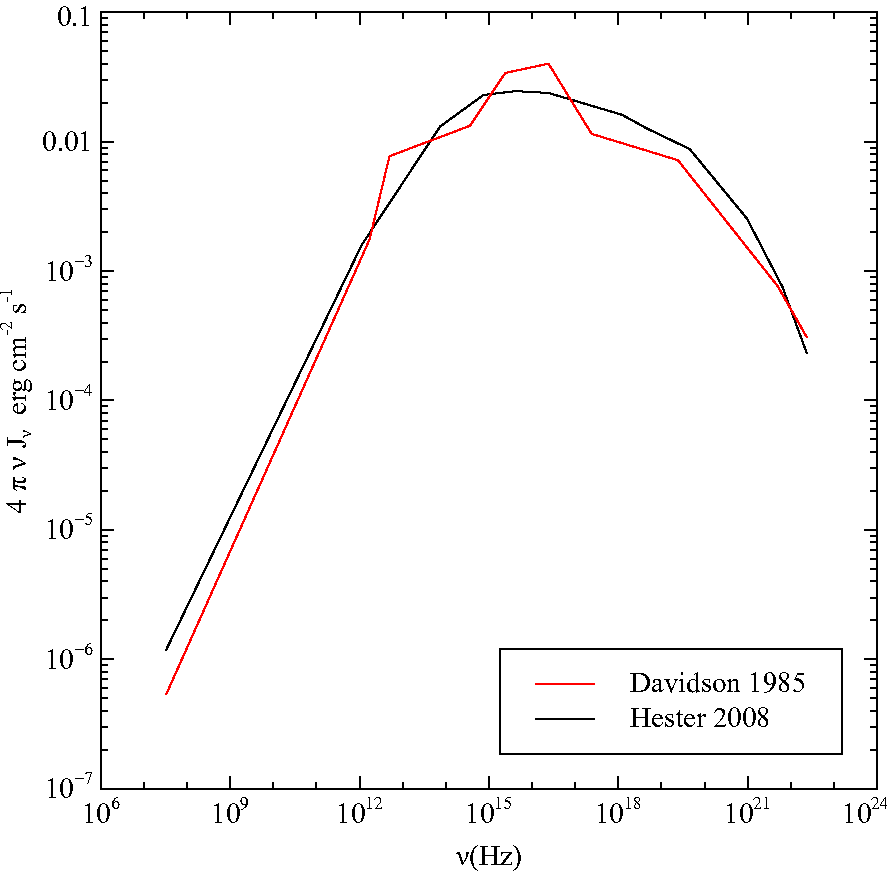
\includegraphics{CrabSED}
\caption[Crab Nebula SED]
{\label{fig:CrabSED}The SEDs produced by the \cdCommand{table Crab} 
commands are compared.
The red line is the SED from \citet{Davidson1985} and 
was the default used
by \Cloudy\ through versions C10.
The black line is the current default, derived by 
\cite{Atoyan.A96On-the-mechanisms-of-gamma-radiation-in-the-Crab}
and shown in \citet{Hester.J08The-Crab-Nebula:-An-Astrophysical-Chimera}}
\end{figure}

According to \citet{Davidson1985}, the total luminosity of the Crab is
$L_{tot} = 10^{38.14}$ \ergps.
The Crab SED could be generated by combining
the commands
\begin{verbatim}
luminosity (total) 38.14
table SED "CrabDavidson.sed"
\end{verbatim}

\subsection{Table SED ``Mrk509.sed''}

This is taken from Figure 3 of \citet{2011A&A...534A..36K}.

\subsection{Table SED ``NGC5548.sed''}

This is taken from the green line in Figure 10 of \citet{2015A&A...575A..22M}.

\subsection{Table SED ``pl1.sed''}

This produces an $f_{\nu} \propto \nu^{-1}$ power-law continuum across the
full spectral range considered by the code.
This should only be used for testing since it may produce unphysically bright 
radio or $\gamma$-ray emission.
See the discussion of the \cdCommand{power law} command on page \pageref{sec:CommandPowerLaw}
for more details, and a safe way to get a power-law continuum.

\subsection{Table SED ``Rubin.sed''}

Nearly all attempts at modeling the Orion Nebula have found that
theoretical stellar atmospheres do not produce enough flux
near 4 Ryd (see,
for example, \citealp{Mathis1982}, 1985; \citealp{Rubin1991};
\citealp{Sellmaier1996}).

Bob Rubin has modified the emergent radiation field from one of the
\citet{Kurucz1979} models to better account for the presence of
high-ionization lines in the Orion Nebula.
This modified SED can be accessed with the
\cdCommand{table SED ``Rubin.sed''} command.
The continuum started life as a
$\log g = 4$, $T_{eff} = 37{,}000$
K Kurucz model, but the flux between 41 eV and 54 eV was raised
by a factor of 11 to reproduce the [Ne III] optical and IR lines.

\subsection{Table SED ``XDR.sed''}

This generates the X-ray SED described in 
\citet{Maloney1996},
%:XDR continuum shape
\begin{equation}
f_{\nu}  = f_0 \times
\left( {\frac{{E }}{{100 \keV}}} \right)^{-0.7} 
[\ergpscmps \Hz^{-1}] ,
\end{equation}
over the energy range 1 -- 100 \keV .
The radiation field has negligible intensity outside this range.

\section{Other Table commands}

\subsection{Overview}

Any of several radiation field shapes that are stored as a permanent part
of the code can be entered with this command.
This is a special version of
the \cdCommand{interpolate} command.
The same interpolation
on a table of input frequencies and fluxes described there is done.
The \cdCommand{table} command can be freely mixed with other
shape commands and a total
of up to 100 \cdCommand{table} and \cdCommand{interpolate} commands
can be entered.

\subsection{Table AGN }
\noindent If the keyword \cdCommand{AGN} appears
(note the presence of a leading space) then
a continuum similar to that deduced by \citet{Mathews1987} will be
used.  The continuum is meant to be similar to typical radio quiet active
galaxies.
The points used to describe this continuum are given in
Table \ref{tab:AGNcontinuum}.

\begin{table}
\centering
\caption{AGN Continuum}
\begin{tabular}{lll}\hline
\label{tab:AGNcontinuum}
$\nu$(Ryd)& log $(F_\nu$)& slope\\
\hline
1.00($-$5)&$-$3.388& $+$2.50\\
9.12($-$3)&4.0115& $-$1.00\\
0.206& 2.6576& $-$0.50\\
1.743& 2.194& $-$1.00\\
4.130& 1.819& $-$3.00\\
26.84& $-$0.6192& $-$0.70\\
7.35($+$3)& $-$2.326& $-$1.67\\
7.40($+$6)& $-$7.34& $-$1.12\\
\hline
\end{tabular}
\end{table}

This radiation field differs from the \citet{Mathews1987} SED
only in that the continuum is assumed to have a sub-millimeter break at
10 microns.
For wavelengths longer than 10\,$\mu$m the continuum is assumed
to have a slope $f_\nu\propto \nu^{+2.5}$,
appropriate for a self-absorbed synchrotron
continuum (\citealp{Rybicki1979}).
Note that this represents a typical
observed continuum,
and may not be directly related to the continuum actually
striking BLR gas \citep{KoristaFerlandBaldwin1997}.

The energy of the sub-millimeter break is not well determined
observationally but has a major impact on high density, high ionization
parameter models, as discussed by \citet{Ferland1989}, \citet{FerlandPeterson1992}, and \citet{Ferland1999a}.  The energy of the infrared break can be
adjusted with the \cdCommand{break} keyword.
The break can be adjusted between the
limits of 0.2 Rydberg and \emm\
by entering the keyword \cdCommand{break}
followed by a number specifying the energy of the break.  The number is
interpreted as the log of the energy in Rydbergs if it is negative and as
linear Rydbergs if positive.  It is interpreted as the linear wavelength
of the break in micron if the keyword \cdCommand{micron} also appears.
If no number appears, but the keywords \cdCommand{no break} does,
then a break at the low-energy
limit of the code (\emm ) is assumed.
The following shows
equivalent ways of generating a continuum with a break at 10 microns;
\begin{verbatim}
table AGN break .00912  # energy in Ryd
table AGN break -2.04   # log of energy in Ryd
table AGN break 10 micron # wavelength in micron
table AGN no break      # no sub-millimeter break
\end{verbatim}
Note that the nature of the SED in AGN is still an open question.  The
shape given here is very simplistic and quite uncertain in the
ionizing ultraviolet.  Moreover, it would not be surprising if the BLR
sees a far different continuum than we do.  This shape may not be
correct for low redshift Seyfert galaxies (\citealp{Binette1989};
\citealp{Clavel1990}) and direct observations of high-redshift quasars
suggest a far softer continuum than this (\citealp{Zheng1997};
\citealp{KoristaFerlandBaldwin1997}).
It is
probably best to only use this shape in exploratory situations and
generate a specific AGN radiation field using either the
\cdCommand{ratio} or \cdCommand{AGN} commands.

\subsection{Table Draine [factor=1.7]}

This enters the galactic background radiation field given by
equation 23 of \citet{Draine1996}.
The radiation field is only defined over a very
narrow wavelength range so it is only appropriate for
certain very simple PDR calculations.
It is shown in Figure \ref{fig:ISM_background} along with the
radiation field produced
by the \cdCommand{table ism} command.
This command specifies both the shape and
intensity of the continuum.

The optional scale factor changes the intensity
of the continuum.
By default it is a linear scale factor but the keyword \cdCommand{log} changes this.

This radiation field is defined up to an energy very close to 1 Rydberg.
It may spill over into the hydrogen-ionizing continuum for certain
choices of the continuum-bin resolution.
Add the \cdCommand{extinguish} command to insure that
H-ionizing radiation is extinguished if this is needed.
The code will print a comment is this is not done.

This continuum should only be used for restricted tests since the vast
majority of the electromagnetic spectrum is undefined.
It was created to compute the Leiden PDR test cases
(the \cdFilename{pdr\_leiden}* simulations in the test
suite) and the paper by \citet{Roellig2007}.

This radiation field is isotropic.
This is an intensity command.

\begin{figure}
\centering
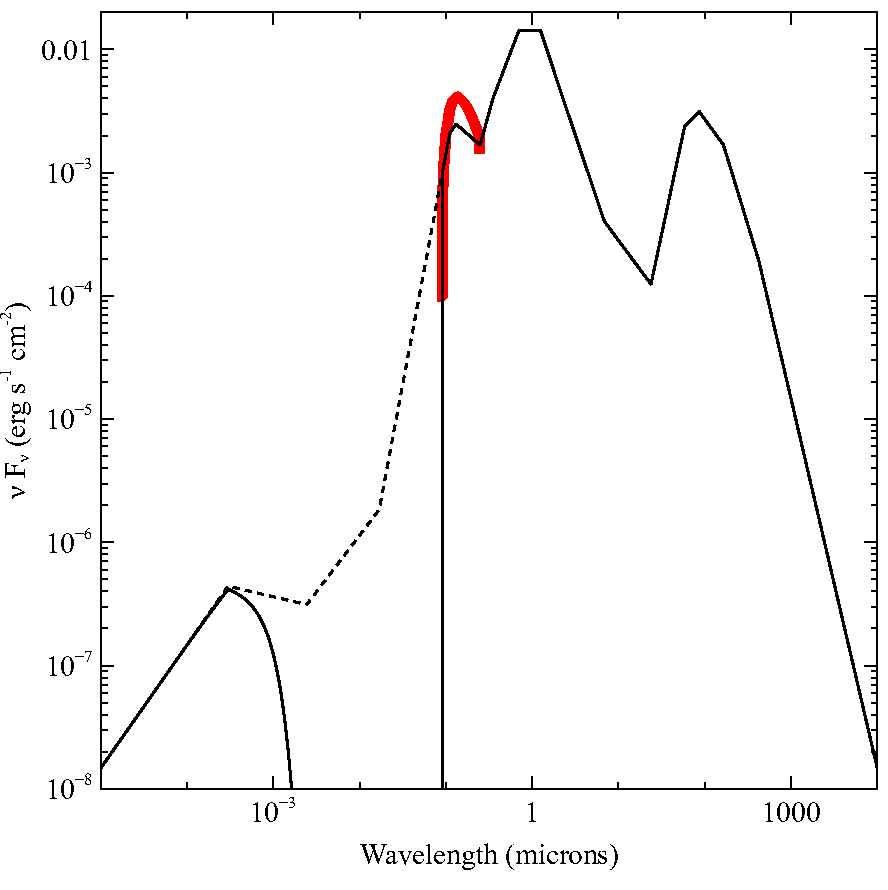
\includegraphics{ism_background}
\caption[ISM radiation field]
{\label{fig:ISM_background}The SED produced by the \cdCommand{table ISM} command is the lighter
line.
The infrared cirrus is the peak at $\lambda \sim  100\,\micron$ and starlight
dominates at shorter wavelengths.
The points just shortward of the Lyman
limit ($0.0912\,\micron$) are interpolated---actually it is thought that interstellar
extinction removes most of this continuum.
The dashed line shows the
interpolated SED and the solid line shows the effects of absorption
introduced by adding the \cdCommand{extinguish} command.
The heavy red line is the \cdCommand{table Draine} continuum. }
\end{figure}

\subsection{Table HM96 [factor=-1]}

This enters the \citet{Haardt1996} background continuum for a redshift
of $z = 2.16$.  This is the original form of the command and is maintained
for reference.  The cosmic microwave background is not included - use the
\cdCommand{CMB} command to add this component.  Note that
this table specifies both the shape and intensity of the radiation field.
There
is an optional multiplicative scale factor to change the intensity.  If
the scale factor is less than or equal to zero then it is interpreted as
the log of the scale factor.

This radiation field is isotropic.
This is an intensity command.

\subsection{Table HM05 redshift 2.21 [quasar; factor=-1]}

This enters the Haardt \& Madau (2005 private communication)
radiation field at any redshift $0 \le z \le 9.479$.  It
interpolates on tables kindly provided by Francesco Haardt.  There are
two forms of the radiation field - the default includes both quasars
and galaxies.  If the keyword \cdCommand{quasar} occurs then a
radiation field considering only quasars is used.  The cosmic
microwave background is not included - use the \cdCommand{CMB} command
to add this component.  Note that this table specifies both the shape
and intensity of the radiation field.  There is an optional
multiplicative scale factor to change the intensity.  If the scale
factor is less than or equal to zero then it is interpreted as the log
of the scale factor.

The radiation field is isotropic.
This is an intensity command.

\subsection{Table HM12 redshift 2.21 [factor=-1]}

This enters the \citet{HaardtMadau2012} radiation field at any redshift $0 \le
z \le 15.93$. It works the same way as the \cdCommand{table HM05} command
described above, except that the keyword \cdCommand{quasar} is not supported
because tables for the quasar-only case do not exist for this data set.

\subsection{Table ism [factor = 0.7]}

The local interstellar radiation field is generated with the keyword
\cdCommand{ism}.
This uses Figure 2 of \citet{Black1987} to represent the
\emph{unextinguished}
local interstellar radiation field (see Figure \ref{fig:ISM_background}).  This command specifies
\emph{both} the shape and luminosity of the radiation field.
The continuum
generated by \Cloudy\ is exactly that given by Black except that the radiation
field between 1 and 4 Ryd is interpolated from the observed or inferred
values.  Actually it is thought that this part of the radiation field is
heavily absorbed by gas in the ISM so that little 1 to 4 Ryd radiation
exists, at least in the galactic plane.  Such absorption can be introduced
with the \cdCommand{extinguish} command.

The \cdCommand{table ism} command also specifies the intensity
of the incident radiation field since this is directly observed.
There is an optional scale
factor to change the intensity of the entire radiation field.
It is the
log of the scale factor if less than or equal to zero and the scale factor
itself if positive.
The actual numbers used by \Cloudy\ to interpolate on
Black's table are given in Table \ref{tab:ISM_Black}.
The frequencies are in Hz, and the
product $\nu f_\nu$ in erg cm$^{-2}$~s$^{-1}$.

This does not include the cosmic microwave background so that it can be used at any redshift.
Use the \cdCommand{CMB}
command to add this component.

\begin{table}
\centering
\caption{ISM Radiation Field}
\label{tab:ISM_Black}\begin{tabular}{llll}\hline
log($\nu$)& log $\nu f_\nu$& log $\nu$& log $\nu f_{\nu}$\\
\hline
9.00& $-$7.93& 14.14& $-$2.30\\
10.72& $-$2.96& 14.38& $-$1.79\\
11.00& $-$2.47& 14.63& $-$1.79\\
11.23& $-$2.09& 14.93& $-$2.34\\
11.47& $-$2.11& 15.08& $-$2.72\\
11.55& $-$2.34& 15.36& $-$2.55\\
11.85& $-$3.66& 15.54& $-$2.62\\
12.26& $-$2.72& 16.25& $-$5.68\\
12.54& $-$2.45& 17.09& $-$6.45\\
12.71& $-$2.57& 18.00& $-$6.30\\
13.10& $-$3.85& 23.00& $-$11.30\\
13.64& $-$3.34\\
\hline
\end{tabular}
\end{table}
The actual ISM radiation field incident on a typical region in the galactic plane could be generated by:
\begin{verbatim}
table ISM
CMB
extinguish column = 22 leak=0
\end{verbatim}

This radiation field is isotropic.
This is an intensity command.

\subsection{Table KS19 redshift 2.21 [factor=-1] [Q=18]}

This enters the \citet{KhaireSrianand2019} extragalactic background radiation
at any redshift $0 \le z \le 15$. It works very similar to the
\cdCommand{table HM12} command described above, except that there is a second
optional parameter giving the integer $Q$ parameter for the requested SED (see
Table~1 of \citealp{KhaireSrianand2019}). When omitted, it will default to
$Q18$, the fiducial model recommended by \citet{KhaireSrianand2019}. If the
$Q$ parameter is included, then adding the scaling factor is mandatory and the
scaling factor should be entered before the $Q$ parameter. Valid values for
the $Q$ parameter are between 14 and 20.

The radiation field is isotropic. This is an intensity command.

\subsection{Table power law [spectral index -1.4, low =.01, hi =20] }

This produces a power-law continuum that is well behaved at both the
high and low energy ends.
The default shape, assumed when no numbers occur
on the command line, is the form $f_\nu   \propto \nu ^\alpha  $.
Here
$\alpha = -1$ for the spectral midrange between 10 microns and 50 keV,
and the continuum has slopes $f_\nu   \propto \nu ^{5/2} $ at lower energies (appropriate for self-absorbed synchrotron, eq 6.54,
p.190, \citealp{Rybicki1979}) and
$f_\nu   \propto \nu ^{ - 2} $ at higher energies.
Note that much of the X-ray literature will use
an implicit negative sign in defining the energy index,
as in equation 13.2 of AGN3.
\Cloudy\ never uses implicit negative signs so a typical AGN will
have an energy index of roughly $-$1.5.
Table \ref{tab:PowerLawContinuum} summarizes the continuum
that is produced by this command if no other parameters are specified.

\begin{table}
\centering
\caption{Power Law Continuum}
\begin{tabular}{ll}\hline
\label{tab:PowerLawContinuum}
$\nu$(Ryd)& slope\\
\hline
1.00($-$8)& $+$2.50\\
9.115($-$3)& $-$1.00\\
3676.& $-$2.\\
7.40($+$6)& $-$\\
\hline
\end{tabular}
\end{table}

Three optional numbers may appear on the command line.
The first number
sets the slope of the mid-range spectral component (infrared to X-ray)
and has a default of -1 ($f_\nu   \propto \nu ^{ - 1} $).
The
next two numbers adjust the energy limits of the mid-range spectral
component.
Their default units are Rydbergs but the keyword \cdCommand{microns} will
change the units to microns \emph{for the first energy only.}
The second number
is the energy (in Rydbergs) of the infrared break.
The default is 0.009115
Ryd (10 microns).
If this second number is zero then the low energy limit
to the continuum (\emm ) will be used.
The number is interpreted
as the log of the energy in Rydbergs if it is negative and linear otherwise.
Note that, with no infrared break, free-free heating will probably be
significant for denser clouds.  A power-law continuum with a low energy
break at 1 micron would minimize this heating and could be generated with
the command
\begin{verbatim}
# a power-law with index -1 and 1 micron break
table power law slope -1, 1 micron break
\end{verbatim}
The following uses the default power law
\begin{verbatim}
# another example, a power-law with index -1
# and 10 micron break, (the default)
table power law slope -1
\end{verbatim}

The third optional number is the energy (in Rydbergs) of the break in
the X-ray continuum.
The default is 50 keV and if it is zero then the
high-energy limit of the continuum (\egamry ) is used.
The number is interpreted as a log if the energy of the
infrared break is entered as
a log and linear otherwise.
The numbers may be omitted from right to left.

\subsection{Table read "contin.txt" [ scale [ = 0.5 ] ]}
\label{sec:CommandTableRead}

This reads in the radiation field predicted from
a previous \Cloudy\ calculation.
The name of the file containing the spectrum predicted
from the first calculation continuum must be enclosed
in a pair of double quotes.
The first calculation saves the radiation
transmitted through a cloud with the
\cdCommand{save transmitted continuum} command described in Section
\ref{sec:CommandSaveTransmittedContinuum}.
Subsequent calculations use the \cdCommand{table read} command
to include this field.

The transmitted spectrum of the first model
will include all transmitted radiation, including line emission, and
will write that out as a single spectral energy distribution. When the
second model reads that in, it will have no knowledge of what was what
in the first model, apart from the outer radius of that model
(assuming a radius was specified in that model).
It will treat it as an incident SED without further
specifics. So the [\oiii ] 5006.84 flux reported by the second model will be
that produced by the second model only, but the 5006.84 photons from the
first model will be included ``anonymously'' in the incident SED.

The \cdCommand{save transmitted continuum} command produces a file containing the frequency in Rydbergs and the transmitted
continuum $\nu f_{\nu}$ [erg cm$^{-2}$ s$^{-1}$].
This continuum is the sum of the attenuated
incident continuum and the fraction of the cloud's diffuse emission
that is transmitted in the outward direction.  The first lines of the 
file contain header information and must not be deleted.

\Cloudy\ checks that the photon energies contained in the
\cdCommand{save transmitted continuum} file are exactly that same as
the photon energies used in the code's internal arrays.  
This is because the contents of the files are simply placed into these arrays with
no interpolation.  You should not try to change the photon energies.

The \cdCommand{table read} command can be freely mixed with all
of the other radiation field shape commands.
Any number of \cdCommand{table read} commands can be entered.\footnote{Only one table read command could be entered in versions
90 and before.}
The \cdCommand{save continuum} file must have been produced by the same version of \Cloudy.

By default, this command does not set the intensity of the radiation
field.  If the \cdCommand{scale} option is not given, the intensity of the
radiation field must be set explicitly, using any of the intensity or
luminosity commands.

If the \cdCommand{scale} option is given, the
intensity scale can be specified relative to the intensity of the previous
calculation.  As with some other \cdCommand{table} commands, the value
specified is interpreted as a log scale if it is non-positive and linear
otherwise. If no number is given, the scale factor defaults to unity.

If the model that generated the transmitted spectrum and the model that reads
it both set a radius, then spherical dilution will implicitly be done. The
scale factor will be a multiplicative factor on top of that, i.e. the
transmitted spectrum will be multiplied by a factor $(r_{\rm out}/r_{\rm
  in})^2 s$ where $r_{\rm out}$ is the outer radius of the first model,
$r_{\rm in}$ is the inner radius of the second model, and $s$ is the scale
factor. A warning will be printed if $r_{\rm in} < r_{\rm out}$, but the
spherical correction will still be done (which would make the radiation field
more intense). If the first model set a radius, but not the second (or {\it
  vice versa}) a caution will be printed and no spherical correction will be
done (but the scale factor will still be applied).

The following gives an example of first creating a file containing the
transmitted radiation field then using this file as the
incident radiation field in a second calculation.
\begin{verbatim}
title this finds transmitted continuum due to warm absorber
hden 9
ionization parameter 1
stop effective column density 21
table AGN
iterate
save transmitted continuum file = "absorber.txt" last
\end{verbatim}
Now use this continuum in a second calculation:
\begin{verbatim}
table read file = "absorber.txt"
luminosity 45
radius 18
hden 9
\end{verbatim}
The output continuum can also be diluted by a factor of 100 compared
to the first calculation:
\begin{verbatim}
table read file = "absorber.txt" scale -2
hden 9
\end{verbatim}

\subsection{Table trapezium}
\label{sec:CommandTableTrapezium}

This enters the radiation field of the Orion Trapezium stars.


\section{Table stars command}
\label{sect:TableStars}

Several sets of emergent SEDs from stellar atmosphere calculations are
accessible.
The command has several sub-keywords that indicate which set
of atmospheres to use. The syntax of the command varies depending on
how the atmosphere grid was constructed. The easiest way to find out
how to use this command is by entering the command \cdCommand{table
star available} after the grids have been installed. The 
\cdCommand{table star} accepts the optional keyword \cdCommand{log}
which indicates that the first number on the line is the logarithm of
that parameter. Usually that is the effective temperature.

Figure \ref{fig:StarsContinuum} compares predictions for
five of the 50~kK SEDs that are
available.  These include a blackbody and atmospheres computed by \citet{Mihalas1972}, \citet{Kurucz1979}, \citet{Kurucz1991} and \citet{Rauch2002}.
All were normalized
to have the same total luminosity ($10^{38}$ erg s$^{-1}$)
observed from a distance of $10^{18}$~cm.
Note the order of magnitude dispersion among the continua for
energies around 4 Ryd.

\begin{figure}
\centering
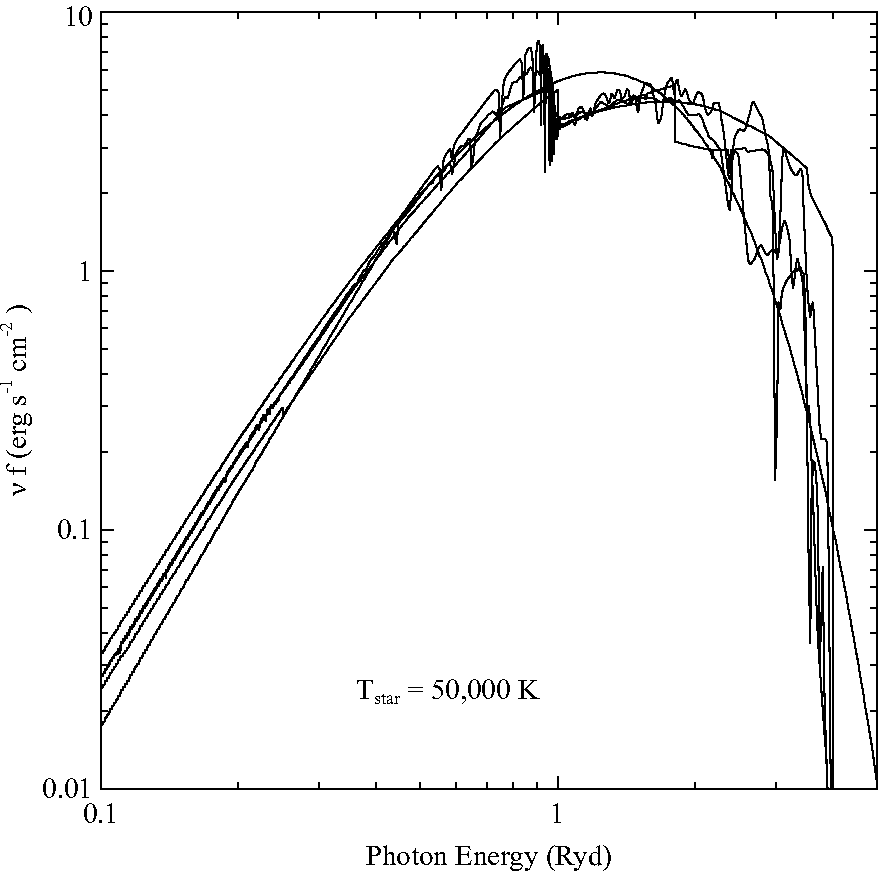
\includegraphics[scale=0.9]{StarsContinuum}
\caption[Stellar radiation fields]
{\label{fig:StarsContinuum}This figure shows the emergent
radiation field predicted by five 50~kK 
stars included with the code.  The smoothest is the blackbody, and the
\citet{Kurucz1991} and \citet{Rauch1997} atmospheres show the most structure.  stars}
\end{figure}

These commands specify only the continuum shape.
It is still necessary to specify a luminosity.
\citet{Tout1996} provide convenient fitting
formulae giving zero age main sequence luminosities as
functions of stellar mass and metallicity.

{\bf Danger!}  Many forms of the \cdCommand{table stars} commands
accept the \cdCommand{log} keyword to indicate that the log of the stellar temperature
is entered.  Many also accept the surface gravity, normally referred to as
``log g'', as a second parameter.  The ``log'' in ``log g'' would cause the
temperature to be interpreted as the log of the temperature.  Either
do not enter the string ``log g'', or write it as ``logg'' or ``log(g)''.

\subsection{Overview of available stellar SEDs}

In versions C06.02 and before the stellar continua were entered into
the code on a case by case basis.
New continua could only be introduced
by writing new code.
Beginning in C07.02 Peter van Hoof developed a unified
treatment so that any continuum could be used by putting
it into a standard format.
This is far more flexible and allows more continua to be entered.

Usually grids have a range of surface temperature, and many also include a
range of surface gravity or metallicity. But other types of parameters are
also possible, e.g., age in the case of stellar population synthesis models.
The \cdCommand{table star} command will interpolate on these tables to
calculate an SED with the specified parameters. More information on the
various grids that are supported can be found on our 
\href{http://gitlab.nublado.org/cloudy/cloudy/-/wikis/StellarAtmospheres}{web site}.

To list all the grids that have already been installed on your system, you can
use the \cdCommand{table star available} command. This will list all the
standard grids that were installed from the webpage above (including their
parameters), but not the custom grids that you created yourself.
The output will also list the \cdCommand{table HM05}
and \cdCommand{table HM12} commands. They are not strictly part of the
\cdCommand{table star} family of commands, but they internally use the stellar
grid infrastructure to do their work.

To list all the SEDs that are contained in a single stellar atmosphere
grid, you can use the \cdCommand{table star $<$grid$>$ list} command. For more
details see our webpage listed above.

\subsection{High-energy component}
\label{sec:StarHighEnergyComponent}

Theoretical stellar atmospheres emit little energy above 4 Ryd while
real OB stars \emph{are} X-ray sources.
\citet{Sciortino1990} find a correlation
between the X-ray and bolometric luminosities which can be fitted~by
\begin{equation}
\log \left( {L_x } \right) = 1.08\left( { + 0.06/ - 0.22} \right)\,\log
\left( {L_{bol} } \right) - 9.38\left( { + 2.32/ - 0.83} \right) .% (25)
\end{equation}
The X-ray luminosity is typically $\sim 6.4$ dex fainter
than the bolometric luminosity.
A source temperature of 0.5 keV is quoted by Sciortino et al.
This X-ray component must be explicitly added as an
independent part of the incident radiation field.
Tests show that the high-energy light has little effect on
conditions in the H~II region but \emph{does} affect the
ionization in the surrounding PDR.

\subsection{Starburst99 files}

It is possible to read in predictions from Starburst99 
(\citealp{Leitherer1999}).\footnote{The \cdCommand{table starburst} command, 
which existed for this purpose in versions through C07, has been replaced
with this  \cdCommand{table stars} command.}
The Starburst99 SEDs are unified with the stellar
atmosphere treatment.
See our web site
\href{http://gitlab.nublado.org/cloudy/cloudy/-/wikis/StellarAtmospheres}{wiki.nublado.org/wiki/StellarAtmospheres} and
Appendix~\ref{ascii} below for more details.

The procedure is to create your Starburst99 calculation on their web site
(we tested the version at STScI).
Store the Starburst99 output file ``*.spectrum1'' as
a file with a ``\cdFilename{.stb99}''  or ``\cdFilename{.stb}'' extension.
Compile it as in the following example
\begin{verbatim}
compile star "some_file.stb99"
\end{verbatim}
You can optionally include the keyword \cdCommand{stellar} or
\cdCommand{nebular} if you want to use only the stellar or the nebular
component of the interstellar radiation field (these are the fourth and fifth
column of the Starburst99 calculation, respectively). The default is to use
the total spectrum, which is the sum of the stellar and nebular component.
This would be the equivalent of including the emission from nearby star
forming regions in your calculation. If you don't want that, you can use the
stellar component only, as in the following example
\begin{verbatim}
compile star "some_file.stb99" stellar
\end{verbatim}
The above commands will produce files \cdFilename{some\_file.ascii} and
\cdFilename{some\_file.idx}, which can then
be used in the \cdCommand{table stars} command:
\begin{verbatim}
table star "some_file.ascii" age=6e7 years
\end{verbatim}

The number on the \cdCommand{table star} command is the
age of the starburst.  It has the same units as the ages given in the
Starburst99 data file and is normally given in years.
It is interpreted as a log if the keyword \cdCommand{log} appears,
and as the linear age otherwise.

It is critical that the original Starburst99 file not be
changed in any way at all.
Doing so will trick the code into generating bogus results.
In any case, it is a good idea to make a plot of the generated
radiation field,
using column 1 and 2 of the output from
the \cdCommand{save continuum} command, to confirm that it is correct.

Starting with the C10 release it is possible to combine several
Starburst99 runs with different metallicities into a single 2-dimensional
grid. This allows interpolation in both age and $\log Z$. This has
to be done by compiling each of the Starburst99 runs as described above
and then manually merging the ``\cdFilename{.ascii}'' files into a single
``\cdFilename{.ascii}'' file. Appendix~\ref{ascii} gives details how the merged
file should be formatted. An example of a merged file is available on the
StellarAtmospheres page of the Cloudy wiki linked at the start of this subsection.
The resulting file can be compiled using
\begin{verbatim}
compile star "merged_file.ascii"
\end{verbatim}
and used as follows
\begin{verbatim}
table star "merged_file.ascii" age=6.7 log(Z)=-1.2
\end{verbatim}

\subsection{PopStar and BPASS grids}

You can convert PopStar and BPASS grids into ``\cdFilename{.ascii}'' files so
that they can be used in \Cloudy. You can either use a single PopStar grid,
allowing interpolation in age, or combine several PopStar grids for the same
initial mass function but different metallicities allowing interpolation in
age as well as $\log Z$. Detailed instructions can be found on
\href{http://gitlab.nublado.org/cloudy/cloudy/-/wikis/StellarAtmospheres}{wiki.nublado.org/wiki/StellarAtmospheres}.
   
\chapter{CHEMICAL COMPOSITION}
% !TEX root = hazy1.tex

\section{Overview}

The default solar composition is summarized in Table
\ref{tab:CompositionSolar}.  C and O abundances come from photospheric
abundances of \citet{Allende2002,Allende2001}, while N, Ne, Mg, Si,
and Fe are from \citet{Holweger2001}.  The helium abundance is a
typical value for nebulae with near-solar compositions.  The remainder
of the first thirty elements comes from \citet{Grevesse1998}.
Meteoritic and photospheric abundances agree for most elements.  They
differ by significant amounts for P, S, Cl, and Mn.  These are fairly
volatile elements so may be deficient in meteorites.  For these four
the means of the meteoritic and photospheric abundances were used.
The default solar abundances are stored in the file
\cdFilename{data/abundances/default.abn} and can be changed
by altering or overwriting that file.

These default abundances are maintained for backwards compatibility.
The \cdCommand{abundances GASS} command described 
in section \ref{sec:2010SolarComposition} will use values from 
\citet{Grevesse2010}.

\begin{table}
\centering
\caption{Default Solar Composition}
\label{tab:CompositionSolar}
\begin{tabular}{lllllll}
\hline
A&&&12+log& log& $n/n$(H)& ref\\
\hline
1& H& Hydrogen& 12.00& 0.00& 1.00E+00& GS98\\
2& He& Helium& 11.00& $-$1.00& 1.00E-01& text\\
3& Li& Lithium& 3.31& $-$8.69& 2.04E-09& GS98\\
4& Be& Beryllium& 1.42& $-$10.58& 2.63E-11& GS98\\
5& B& Boron& 2.79& $-$9.21& 6.17E$-$10& GS98\\
\hline
6& C& Carbon& 8.39& $-$3.61& 2.45E-04& AP02\\
7& N& Nitrogen& 7.93& $-$4.07& 8.51E-05& H01\\
8& O& Oxygen& 8.69& $-$3.31& 4.90E-04& AP01\\
9& F& Fluorine& 4.48& $-$7.52& 3.02E-08& GS09\\
10& Ne& Neon& 8.00& $-$4.00& 1.00E-04& H01\\
\hline
11& Na& Sodium& 6.33& $-$5.67& 2.14E-06& GS98\\
12& Mg& Magnesium& 7.54& $-$4.46& 3.47E-05& H01\\
13& Al& Aluminium& 6.47& $-$5.53& 2.95E-06& GS98\\
14& Si& Silicon& 7.54& $-$4.46& 3.47E-05& H01\\
15& P& Phosphorus& 5.51& $-$6.50& 3.20E-07& GS98*\\
\hline
16& S& Sulphur& 7.27& $-$4.74& 1.84E-05& GS98*\\
17& Cl& Chlorine& 5.28& $-$6.72& 1.91E-07& GS98\\
18& Ar& Argon& 6.40& $-$5.60& 2.51E-06& GS98\\
19& K& Potassium& 5.12& $-$6.88& 1.32E-07& GS98\\
20& Ca& Calcicum& 6.36& $-$5.64& 2.29E-06& GS98\\
\hline
21& Sc& Scandium& 3.17& $-$8.83& 1.48E-09& GS98\\
22& Ti& Titanium& 5.02& $-$6.98& 1.05E-07& GS98\\
23& V& Vanadium& 4.00& $-$8.00& 1.00E-08& GS98\\
24& Cr& Chromium& 5.67& $-$6.33& 4.68E-07& GS98\\
25& Mn& Manganese& 5.46& $-$6.54& 2.88E-07& GS98*\\
\hline
26& Fe& Iron& 7.45& $-$4.55& 2.82E-05& H01\\
27& Co& Cobalt& 4.92& $-$7.08& 8.32E-08& GS98\\
28& Ni& Nickel& 6.25& $-$5.75& 1.78E-06& GS98\\
29& Cu& Copper& 4.21& $-$7.79& 1.62E-08& GS98\\
30& Zn& Zinc& 4.60& $-$7.40& 3.98E-08& GS98\\
\hline
\end{tabular}\\[0.5pc]
References: GS98: \citet{Grevesse1998}, GS98* - mean of photospheric
and meteoritic, H01: \citet{Holweger2001}, AP01, AP02
\citet{Allende2001,Allende2002}.
\end{table}

Abundances are always specified by \emph{number} relative to
\emph{hydrogen,} not by mass or relative to silicon.
Abundances are relative to the total hydrogen
density, the sum of H in atomic, ionic, and molecular form.
These are gas-phase abundances
and do not include material locked into grains.
The
composition will be printed in the header information that starts the
printout.
You should check this to confirm that the right composition is
used.

The following sections describe how to modify the chemical composition.

\section{Absolute abundances and scale factors }

Abundances can be specified as either \emph{absolute abundances} or as
\emph{scale factors.}
An absolute abundance gives the abundance of an element relative
to hydrogen.
An example might be $n(\mathrm{O} ) /n( \mathrm{H} ) = 4 \times 10^{-4}$.
A relative abundance
is given relative to another value.
An example might be the abundance
relative to the solar value, $n(\mathrm{O}) / n(\mathrm{H}) = 4 \times
[n(\mathrm{O})/n(\mathrm{H})]_\odot$.

\section{Precedence}

There are many ways to specify an abundance.
It is even possible to specify different abundances for the
same element in the same input script.
If the absolute abundance is specified with more than one command then
the last abundance is used.
If the abundance is specified by both its
absolute abundance and by a scale factor then both are used.
Either of
the following will multiply the default \hii\ region nitrogen abundance by
a factor of two:
\begin{verbatim}
abundances H II region
element scale factor nitrogen 2
\end{verbatim}
or
\begin{verbatim}
element scale factor nitrogen 2
abundances H II region
\end{verbatim}
The \cdCommand{element scale factor} option applies a scale factor
while the
\cdCommand{element abundance} option sets an absolute abundance.
The \cdCommand{abundances \hii\ region}
command uses one of the absolute abundance mixtures that are stored
by the code.
This command enters the gas-phase
abundances of all \LIMELM\ elements and also includes interstellar grains.
The \cdCommand{element} command changes some details about a particular element.

In the following example both commands set absolute abundances so the
first nitrogen \cdCommand{abundance} will have no effect and the final nitrogen abundance
will be the default \hii\ region abundance
\begin{verbatim}
element abundance nitrogen -4.7
abundances H II region
\end{verbatim}
In the following only the second nitrogen scale factor has any
effect since the second scale factor overwrites the first:
\begin{verbatim}
element scale factor nitrogen 3
element scale factor nitrogen 2
abundances H II region
\end{verbatim}
The result will be \hii\ region abundances with nitrogen having twice its
normal value.
Similarly, the combination
\begin{verbatim}
element abundance nitrogen -4
element scale factor nitrogen 2
\end{verbatim}
in either order would result in
$n(\mathrm{N})/n(\mathrm{H}) = 2\times10^{-4}$ since the first command
sets an absolute abundance of $10^{-4}$ and the second command
doubles this.

The chemical composition is printed at the start of the calculation.
Be sure to confirm that the composition has been entered correctly.

\section{Abundances he c\dots}
\label{sec:CommandAbundances}

The abundances of all elements can be entered with the command
\cdCommand{abundances}
followed by:
a) a complete set of abundances,
b) the keyword \cdCommand{all} and
a single number to set all of the abundances,
or c) a second keyword to select
one of the stored abundance sets.

\subsection{Arbitrary abundances}

The \cdCommand{abundances} command can be used to specify the abundances of
a number of elements in one command.
The composition can be
specified on several lines with \cdCommand{continue} lines
following the initial \cdCommand{abundances} line.
Abundances of zero are not allowed; \Cloudy\ will stop if
they are entered.
Elements can be turned off with the \cdCommand{elements off} command.

The element symbol must be written before its abundance to identify
what element the value belongs to. An optional equals sign is allowed
in between the symbol and the value to improve readability.
The abundances can be entered in any order.

The best way to enter abundances is as \emph{absolute abundances},
as in the following example
\begin{verbatim}
abundances he =-1 li =-9   be =-11 b  =-9 c  =-4.3 n  =-5 o  =-2.3
continue    f =-7 ne =-1.2 na =-3  mg =-8
continue   al =-8 si =-8   p  =-6  s  =-8 cl =-9   ar =-8 k  =-6
continue   ca =-8 sc =-9   ti =-7  v  =-8 cr =-6.3 mn =-6 fe =-8
continue   co =-9 ni =-8   cu =-7  zn =-7
\end{verbatim}
The abundances can also be entered as a set of scale factors indicating
the desired abundances relative to the current set absolute abundance.
These will be solar by default.
The following example doubles the oxygen
abundance and lowers the iron abundance
\begin{verbatim}
abundances he =1 li =1 be =1 b  =1 c  =1 n  =1 o  =2
continue   f  =1 ne =1 na =1 mg =1
continue   al =1 si =1 p  =1 s  =1 cl =1 ar =1 k  =1
continue   ca =1 sc =1 ti =1 v  =1 cr =1 mn =1 fe =0.0000001 #deplete iron
continue   co =1 ni =1 cu =1 zn =1
\end{verbatim}
It is better to specify absolute abundances since the default solar
composition changes from time to time.

The code checks the sign of all of the entered abundances to decide
which style was entered.
The numbers are interpreted as linear scale factors
if \emph{all} are positive,
and as logs of the abundance relative to hydrogen if
\emph{any} are negative.

\subsection{Setting all at once}

If the keyword \cdCommand{all} appears and exactly one number
is entered then all
of the elements heavier than hydrogen are given this absolute abundance.
The number is the log of the abundance if it is less than or equal to zero
and the abundance itself if it is positive.
Either of the following commands
will give all elements between and including helium and zinc an absolute
abundance of $10^{-10}$ by number relative to hydrogen:
\begin{verbatim}
abundances all -10
abundances all 1e-10
\end{verbatim}
The \cdCommand{metals} command will set abundances
of all elements heavier than helium.

\subsection{Abundance ``filename.abn'' -- using tables of abundances}

A set of abundances stored in an external file are used if there are no numbers on the
\cdCommand{abundances} command but a file name 
occurs in quotation marks. 
The following gives some examples:
\begin{verbatim}
abundances "cameron.abn"
abundances "HII.abn" no grains
\end{verbatim}


Table \ref{tab:AbundanceSetsStored} lists some of the abundance sets
that are included in the distribution.
The keyword given in the first column of Table \ref{tab:AbundanceSetsStored}
can be used rather than the filename.  
This maintains compatibility with versions C13 and before.
This abundance sets in this table have been part of the code's distribution for a number of years
and more recent sets are not listed here.
Do a listing of the \cdFilename{*.abn} files in  \cdFilename{data/abundances}
to get a full list of the available abundances.

\begin{table}
	\small
	\centering
	\caption{Stored Abundance Sets}
	\label{tab:AbundanceSetsStored}\begin{tabular}{llp{6cm}l}
	\hline
	Keyword		& Filename			& Description					& grains? \\
	\hline
			& \cdFilename{default.abn}	& The default abundances				& no \\
	CAMEron		& \cdFilename{Cameron.abn}	& These are from \citet{Cameron1982}.			& no \\
	PRIMordial	& \cdFilename{primordial.abn}	& The primordial abundances.				& no \\
	CRAB		& \cdFilename{crab.abn}		& These are from model M1, Table 3, of
							  \citet{PequignotDennefeld1983}.			& no \\
	NOVA		& \cdFilename{nova.abn}		& These are roughly those derived by
							  \citet{Ferland1978}.					& no \\
	\hii, ORIOn	& \cdFilename{hii.abn}		& The \hii\ region abundances are the mean of the Orion
							  Nebula abundances given in three studies.		& Orion \\
	AGB, PLANetary	& \cdFilename{pn.abn}		& These abundances are from \citet{Aller1983} and
							  \citet{Khromov1989}, with high depletions assumed for
							  elements they do not list.				& ISM \\
	ISM		& \cdFilename{ism.abn}		& The gas-phase abundances are an average for the warm
							  and cold phases of the interstellar medium.		& ISM \\
	OLD SOLAR 84	& \cdFilename{solar84.abn}	& The composition will be the solar used in versions
							  84--94 of the code.  These are defined in Table
							  \ref{tab:CompositionSolarOld} and were taken from the
							  meteoritic abundances of \citet{Grevesse1989} with
							  extensions by \citet{Grevesse1993}.  All three of the
							  keywords \cdCommand{old solar 84} must appear.	& no \\
	GASS		& \cdFilename{solar\_GASS10.abn}& This will use solar abundances
							  \label{sec:2010SolarComposition} from
							  \citet{Grevesse2010}. The abundances are listed in
							  Table \ref{tab:2010SolarComposition}.			& no \\
	ALLEn		& \cdFilename{allen73.abn}	& These are the cosmic abundances of \citet{Allen1973}.	& no \\
	\hline
	\end{tabular}
\end{table}

Some of the stored abundance sets include grains, as indicated in Table \ref{tab:AbundanceSetsStored}.
The \cdCommand{no grains} and \cdCommand{no QHeat} options are recognized,
as described on the \cdCommand{grains} command (see section \ref{sec:GrainsCommand}).
For instance, ISM abundances but Orion grains would be specified with the combination
\begin{verbatim}
grains Orion
abundances "ISM.abn" no grains
\end{verbatim}
Because of the ability to use keywords, this is equivalent to
\begin{verbatim}
grains Orion
abundances ISM no grains
\end{verbatim}

The abundances files contain lines giving the name of an element and its abundance relative 
to hydrogen. 
Hydrogen may be in specified, or may not be.  If the abundance of hydrogen is 
given and is not equal to unity the code will rescale the abundances by the entered value 
for hydrogen.  If hydrogen is not specified it is assumed to have an abundance
of 1.

All elements heavier than hydrogen are turned off before the abundance files are read.
An element is turned on if it appears in the file.
If an element is not included in the file it will not be included in the calculation.

The \cdCommand{abundances} command has a \cdCommand{print} option to report
grain types and abundances entered for each active element.

\subsection{Older solar abundances}

The default solar abundances are stored in the file 
\cdFilename{data/abundances/solar.abn} and can be changed
by altering or overwriting that file.

The keyword \cdCommand{old solar 84} uses the solar composition
used in versions 84 - 94 of the code.
These are defined in Table \ref{tab:CompositionSolarOld}
and were taken from the
meteoritic abundances of \citet{Grevesse1989} with extensions by
\citet{Grevesse1993}.
The keyword \cdCommand{Cameron} uses the \citet{Cameron1982}
abundances.
The keyword \cdCommand{Allen} uses the \citet{Allen1973} abundances.
These are maintained for historical reasons.

\begin{table}
\centering
\caption{Old Solar Composition, default in versions C84 - C94}
\label{tab:CompositionSolarOld}
\begin{tabular}{llllll}
\hline
&&&&Solar\\
\hline
1& H& Hydrogen& 1& 0.00& 12.00\\
2& He& Helium& 0.1& $-$1.00& 11.00\\
3& Li& Lithium& 2.04E-09& $-$8.69& 3.31\\
4& Be& Beryllium&  2.63E-11& $-$10.58&1.42\\
5& B& Boron&  7.59E-10& $-$9.12&2.88\\
\hline
6& C& Carbon&  3.55E-04&$-$3.45& 8.55\\
7& N& Nitrogen& 9.33E-05& $-$4.03& 797\\
8& O& Oxygen& 7.41E-04& $-$3.13& 8.87\\
9& F& Fluorine& 3.02E-08&  $-$7.52&4.48\\
10& Ne& Neon& 1.17E-04& $-$3.93& 8.07\\
\hline
11& Na& Sodium& 2.06E-06& $-$5.69& 6.31\\
12& Mg& Magnesium& 3.80E-05& $-$4.42& 7.58\\
13& Al& Aluminium& 2.95E-06& $-$5.53& 6.47\\
14& Si& Silicon& 3.55E-05& $-$4.44& 7.55\\
15& P& Phosphorus& 3.73E-07& $-$6.43& 5.57\\
\hline
16& S& Sulphur& 1.62E-05& $-$4.79& 7.21\\
17& Cl& Chlorine& 1.88E-07& $-$6.73& 5.27\\
18& Ar& Argon& 3.98E-06& $-$5.40& 6.60\\
19& K& Potassium& 1.35E-07& $-$6.87& 5.13\\
20& Ca& Calcicum&  2.29E-06&$-$5.64& 6.36\\
\hline
21& Sc& Scandium&  1.58E-09&  $-$8.80& 3.20\\
22& Ti& Titanium&  1.10E-07& $-$6.96& 5.04\\
23& V& Vanadium& 1.05E-08& $-$7.98& 4.02\\
24& Cr& Chromium&  4.84E-07& $-$6.32& 5.68\\
25& Mn& Manganese& 3.42E-07& $-$6.47& 5.53\\
\hline
26& Fe& Iron& 3.24E-05& $-$4.49& 7.51\\
27& Co& Cobalt&  8.32E-08& $-$7.08& 4.92\\
28& Ni& Nickel&  1.76E-06& $-$5.75& 6.25\\
29& Cu& Copper& 1.87E-08& $-$7.73& 4.27\\
30& Zn& Zinc& 4.52E-08& $-$7.34& 4.66\\
\hline
\end{tabular}
\end{table}

\begin{table}
\centering
\caption{2010 Solar Composition, keyword \protect\cdCommand{GASS}}
\label{tab:2010SolarComposition}
\begin{tabular}{lllll}
\hline
&&&Solar\\
\hline
1& H& 1& 0& 12\\
2& He& 8.51E-02& -1.07& 10.93\\
3& Li& 1.12E-11& -10.95& 1.05\\
4& Be& 2.40E-11& -10.62& 1.38\\
5& B& 5.01E-10& -9.3& 2.7\\
6& C& 2.69E-04& -3.57& 8.43\\
7& N& 6.76E-05& -4.17& 7.83\\
8& O& 4.90E-04& -3.31& 8.69\\
9& F& 3.63E-08& -7.44& 4.56\\
10& Ne& 8.51E-05& -4.07& 7.93\\
11& Na& 1.74E-06& -5.76& 6.24\\
12& Mg& 3.98E-05& -4.4& 7.6\\
13& Al& 2.82E-06& -5.55& 6.45\\
14& Si& 3.24E-05& -4.49& 7.51\\
15& P& 2.57E-07& -6.59& 5.41\\
16& S& 1.32E-05& -4.88& 7.12\\
17& Cl& 3.16E-07& -6.5& 5.5\\
18& Ar& 2.51E-06& -5.6& 6.4\\
19& K& 1.07E-07& -6.97& 5.03\\
20& Ca& 2.19E-06& -5.66& 6.34\\
21& Sc& 1.41E-09& -8.85& 3.15\\
22& Ti& 8.91E-08& -7.05& 4.95\\
23& V& 8.51E-09& -8.07& 3.93\\
24& Cr& 4.37E-07& -6.36& 5.64\\
25& Mn& 2.69E-07& -6.57& 5.43\\
26& Fe& 3.16E-05& -4.5& 7.5\\
27& Co& 9.77E-08& -7.01& 4.99\\
28& Ni& 1.66E-06& -5.78& 6.22\\
29& Cu& 1.55E-08& -7.81& 4.19\\
30& Zn& 3.63E-08& -7.44& 4.56\\
\hline
\end{tabular}
\end{table}

\subsection{Grains, gas-phase depletions, and quantum heating}

Certain elements, especially Si, Ca, Al, Mg, and Fe,
are heavily depleted
onto grains in the ISM.
\citet{KingdonFerlandFeibelman1995} discuss the observational
effects of grains upon an \hii\ region.
The abundance sets specified by the
\cdCommand{H II region},
\cdCommand{ISM}, or \cdCommand{planetary nebula} keywords
will include grains and the gas-phase
mixtures given in Table \ref{tab:AbundanceSetsStored}.
The bottom line of the table lists the type
of grains that are included by default.
These types are defined in the section on grains
starting on page \pageref{sec:GrainsCommand}.

Grains can also be specified separately with the
\cdCommand{grains} command (see section \ref{sec:GrainsCommand}).
If you use the \cdCommand{grains} command to specify another type
of grains then you should include the keyword
\cdCommand{no grains} on the abundances
line to prevent the default grains from also being used.

If you set the keyword \cdCommand{no grains} to not include
the default grains and
do not specify another set of grains with the
\cdCommand{grains} command then grains
will not be included in the calculation but the depleted
gas-phase abundances
will still be used.\footnote{In versions 77 and before,
the abundances of depleted elements were
set to solar values when \cdCommand{no grains} was set.}
This is, of course, not self-consistent.

Quantum or single-photon heating will be considered for all
grain species where it will be important.
Quantum heating only affects the Wien tail of the grain
thermal-emission spectrum but is computationally fairly expensive.
The \cdCommand{no qheat} option on the \cdCommand{abundances} command
will disable quantum heating.
Figure \ref{fig:grains_qheat} compares the continuum predicted
in the test case \cdFilename{grains\_qheat},
a part of the code's test suite.
Quantum heating is normally
included and the \cdCommand{no qheat} option was used to
disable it to make this comparison.

To access the full range of grain options it is best to combine the \cdCommand{no grains}
option on the \cdCommand{abundances} command and follow that with
the \cdCommand{grains} command and its options,
described in section \ref{sec:GrainsCommand}), as in
\begin{verbatim}
abundances ISM no grains
grains [options]
\end{verbatim}

\begin{figure}
\centering
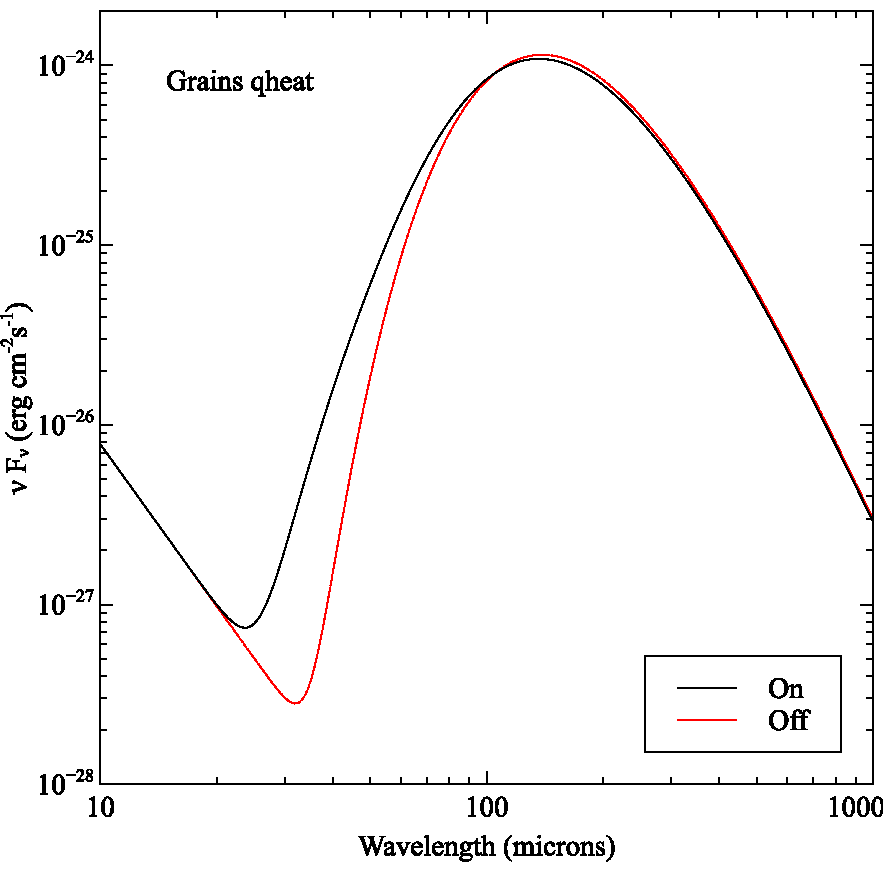
\includegraphics{grains_qheat}
\caption[Quantum heating]{\label{fig:grains_qheat}This figure shows the
net emission computed by the test case
\cdFilename{grains\_qheat.}
The solid line includes quantum heating while the dashed
line has disabled~it. The emission lines have been suppressed in this plot for clarity.}
\end{figure}
% this figure generated with the docs/latex/hazy1/grains_qheat* files
% grains_qheat.in was from tsuite/auto at time of this revision
% run both grains_qheat*.in files, open Veusz file grains_qheat.vsz
% and update data to regenerate Figure.  Export to
% grains_qheat.pdf to update figure in Hazy1

\subsection{Interactions between the abundances and grains commands}

It is possible to include grain species with both the
\cdCommand{abundances} command,
described here, and with the \cdCommand{grains} command.
For simplicity you should only set the grain abundances
only once.
If you specify the same grains more than one time you are asking
for trouble.
The rules for how these commands interact are described elsewhere.

You should check that you have the expected grain abundances by looking
at the list of grain abundances given at the start of the calculation and
at the value of $A_V/N_{\mathrm{H}}$ given at the end.

\section{Abundances starburst, Z=10}

This form of the \cdCommand{abundances} command interpolates on
Fred Hamann's grid
of abundances for an evolving starburst in a massive galactic core.
The
chemical evolution model is more fully described by \citet{Hamann1993}.
This grid is model M5a of that paper.
It uses a star formation
rate and infall timescales very close to, but slightly faster than,
the
``standard'' elliptical model (see also \citealp{Arimoto1987,Matteucci1986,Matteucci1987,Bica1988}).
Its IMF also
has a slope very similar to, but slightly steeper than
($x = 1.0$ instead of 1.1), that of the standard elliptical model.
The main difference is
that the IMF has a lower mass cutoff at $M = 2.5 M_\odot$ instead of
$\sim 0.1 M_\odot$ in the standard models.
This allows the gas to reach much higher metallicities
before the gas is locked up in low-mass stellar remnants.

The metallicity of the gas relative to solar appears on the line.
It is interpreted as the log of the metallicity if it is
less than or equal
to zero, and the linear metallicity if positive.
The keywords
\cdCommand{log} or \cdCommand{linear}
will force the number to be interpreted appropriately.
The limits to the
range of possible metallicities are $10^{-3} Z_{sun}$ and $36 Z_{sun}$.

This command works by generating scale factors that multiply
the current standard abundance.
This is solar by default.
The command does not derive
absolute abundances.
If you change the abundances with a second
\cdCommand{abundance}
command then the scale factors will multiply those new abundances.

The keyword \cdCommand{trace} will print the abundances of
all elements as a function
of metallicity between the full $10^{-3} Z_{sun}$ and
$36 Z_{sun}$ limits.
The code will then stop.

\section{Abundances isotopes}

Isotope fractions may be specified with this command by providing
one of the keywords entered in Table~\ref{tab:isotopes}, or a
filename enclosed in double-quotations.
Note that all tables rely on the \citet{Rosman1998}
terrestrial abundances for many isotopes.
For instance, \citet{Asplund2009} make use of the
``representative isotopic composition'', while \citet{Lodders2003}
opts for the ``best measurement from a single terrestrial source''.
By default, the abundances of \citet{Asplund2009} are used,
modified to match the primordial D/H ratio of $1.65 \times 10^{-5}$
(\citealp{Pettini2001}), and to reproduce Cloudy's historic 13C isotope
fraction of 1/30.

\begin{table}
\centering
\caption{Isotope Fractions Data}
\label{tab:isotopes}
\begin{tabular}{llll}
\hline
Keyword		& Filename		& Abundance Type	&	Reference		\\
\hline
aspl		& ``Asplund09-iso.abn''	& Protosolar		&	\citet{Asplund2009}	\\
lodders09	& ``Lodders09-iso.abn''	& Protosolar		&	\citet{Lodders2009}	\\
lodders03	& ``Lodders03-iso.abn''	& Solar System		&	\citet{Lodders2003}	\\
rosm		& ``Rosman98-iso.abn''	& Terrestrial 		&	\citet{Rosman1998}	\\
    		& ``default-iso.abn''	& aspl + D/H + f(13C)	&				\\
\hline
\end{tabular}
\end{table}

Additional isotopic data used internally include masses
derived from \citet{Audi1995}, and spins and magnetic
moments obtained from \citet{Stone2005}.

Note that the command automatically resets the Deuterium
and 13C abundances.
The command \cdCommand{element name isotopes}, described
below, should be issued to maintain a desired isotope ratio,
following all instances of \cdCommand{abundances isotopes}.

A user-defined file must include fractions for all
the isotopes present in the default files.

\par
The default isotope abundances were used in our predictions
for hyperfine structure line emission from hot and rarefied
media, e.g., the intracluster medium in galaxy clusters, and
the Orion million K gas; these are discussed in detail in
\citet{Chatzikos2014}.

\section{Element name [scale, abundance, isotopes, off, log, table]}

This sets the abundance of a particular element.
The command has several
keywords that change the behavior of the command.

\subsection{Element name scale}

If the keyword \cdCommand{scale} appears
then the number on the line is a scale factor
multiplying the current abundance of the element.
The number is a linear
scale factor if it is positive or if the \cdCommand{linear}
keyword appears and it is
the log of the scale factor if the number is negative.
If the key \cdCommand{log}
appears (note the leading space) then the scale factor
is interpreted as
a log irregardless of its sign.

\subsection{Element name abundance}

If \cdCommand{abundance} appears then the number is
the absolute abundance of the
element by number relative to hydrogen.
The number is the log of the
abundance unless the \cdCommand{linear} keyword appears.

\subsection{Element name isotopes}

If the keyword \cdCommand{isotopes} appears, then
the code expects a pair of numbers, the atomic mass
number and the isotope fraction, for each of the
elemental isotopes.
Linear numbers are expected.

\subsubsection{Setting the D/H ratio}

This command should be used to set the D/H abundance ratio.
For example, the following sets the ratio to $2\times 10^{-5}$,
close to the current solar-system value:
%
\begin{verbatim}
element hydrogen isotopes (1, 1) (2, 2e-5)
\end{verbatim}

This mainly affects HD cooling.
The default is the primordial abundance of $1.65 \times 10^{-5}$
as measured by \citet{Pettini2001}.

The command \cdCommand{set D/H} has been deprecated.

\subsubsection{Setting the 12C/13C ratio}

This command should be used to set the 12C/13C ratio.
For instance, the following sets the ratio to 5:
%
\begin{verbatim}
element carbon isotopes (12, 5) (13, 1)
\end{verbatim}
%

The code currently predicts the $^{13}$CO rotation spectrum
and the intensity of
$^{13}\ciii\ \lambda 1910$\AA\ (\citealp{Clegg1997}) using this ratio.
The code does not now solve
for $^{12}$C and $^{13}$CO abundances and ionic fractions
but rather assumes that
the ratio $^{12}$CO/$^{13}$CO and the
$^{12}$C$^{+2}/^{13}$C$^{+2}$ ionization fractions are equal to
$^{12}$C/$^{13}$C.
This ignores chemical fractionation.
A full treatment of this physics is high on the list of priorities.

The $^{12}$C/$^{13}$C ratio depends on both location in the
galaxy and age.
It is $\approx 90$ in the solar system (\citealp{Asplund2009})
and reflects the galactic value when the sun formed.
The value toward the Galactic center
is about 20 increasing to $\approx77$ at the solar radius
(\citealp{Wilson1994}).
The default value of 30 is a compromise.

The command \cdCommand{set 12C13C} has been deprecated.

\subsection{Element isotopes all}

This command enables the available isotopologues of all molecules.
Currently, only singly-substituted isotopologues are available in
Cloudy.
Densities are simply scaling by fractionations of constituent elements.

Deuterium is not presently enabled by this command.
Isotopes of all other elements are enabled.

The command \cdCommand{set isotopes all} has been deprecated.

\subsection{Element name ionization }

This allows the ionization distribution of an element to be set.
Each
number is the ionization fraction, $n(A^{+i})/n(A)$,
for successive stages of
ionization.
The code will scan off up to A+1 numbers, where A is the atomic
number of the element.
If any numbers are negative then all are interpreted
as logs of the ionization fraction.
If there are fewer than A+1 numbers
then the missing stages of ionization are assumed to have zero abundance.

The total density of all ions must add up to the total density of the element.
The code imposes several particle conservation rules to insure that
mass is conserved.
The density of the ions will be renormalized so that the
total abundance of the element is equal to the value
specified by other commands.\footnote{In versions C08 and before this
command did not confirm that the sum of the ionization fractions
was unity.  The abundance of each stage of ionization was set to the product
of the ionization fraction times the abundance set by other commands.  If the
fractions did not add up to unity the effect was to change the total
abundance of the element.}

This command does not specify the chemical state.
The \htwo\ fraction can
be set with the \cdCommand{set H2} command.
Chemistry is disabled if you set the ionization distribution of an element
that is part of the chemical network.
It will not be possible to obtain
a chemical solution if the abundances of the atom and ions cannot respond
to changes in the chemistry.

All of this is unphysical and is only intended as a way to test the code.

\subsection{Element name off}

If the keyword \cdCommand{off} appears
(note the leading space) then the element
is not included in the calculation.
The ionization equilibrium, opacity,
and cooling due to the element will not be computed.

The keyword \cdCommand{on} will include an element that was
previously turned off in the same input stream.

You can save computer time if you turn an element off.
This is especially
true for third- and fourth-row elements.
These take longer to compute
because of the large number of inner-shell electrons.
They often have
negligible effects on the thermal and ionization structure because of
their low abundances.

Memory for the species that are present is dynamically allocated when
the code starts.
When the code is used to compute a large grid of models
it is not possible to turn on an element that was turned off for the first
model since the needed memory does not exist.
You can turn off an element
in later models since the element is simply not computed.
In later
calculations in a grid the code will ignore any attempt to turn on an
element that was initially turned off.

The chemical solution may become destabilized if an element that forms
molecules is turned off.
Do not turn off elements that are part of the
chemistry if the calculation extends into a PDR or molecular cloud.
The
code will generate a warning if this is done.

Turning off an element with this command has other side effects.
For instance, the following input stream would produce unexpected results:
\begin{verbatim}
element zinc ionization -3 0 -4
init "ism.ini"
element zinc on
\end{verbatim}
because the \cdFilename{ism.ini} file turns off zinc.
This destroys the memory of the
\cdCommand{element zinc ionization} command,
which sets the ionization of the element.
So, when the element is turned back on with the
\cdCommand{element zinc on} command
the ionization will be determined self consistently rather than set to the
constant values.

\subsection{Element limit off -12}
\label{sec:ElementLimitOffCommand}

\noindent Elements with abundances that are
smaller than the number on the line will be ignored.
The number is the log of the limiting abundance by number relative to
hydrogen.
This is an easy way to turn off elements that have trivial
abundances.
Table \ref{tab:CompositionDecreasingOrder} lists the elements
in terms of decreasing abundance.
The command
\begin{verbatim}
elements limit off -7
\end{verbatim}
would cause all elements at Cobalt and above in
Table \ref{tab:CompositionDecreasingOrder} to be turned off.

\begin{table}
\centering
\caption{Solar composition sorted by abundance}
\begin{tabular}{llll}
\hline
\label{tab:CompositionDecreasingOrder}
A& Symbol& Name& log $n(x)/n(\mathrm{H})$\\
4& Be& Beryllium& -10.58\\
5& B& Boron& -9.21\\
21& Sc& Scandium& -8.83\\
3& Li& Lithium& -8.69\\
23& V& Vanadium& -8.00\\
29& Cu& Copper& -7.79\\
9& F& Fluorine& -7.52\\
30& Zn& Zinc& -7.40\\
27& Co& Cobalt& -7.08\\
22& Ti& Titanium& -6.98\\
19& K& Potassium& -6.88\\
17& Cl& Chlorine& -6.72\\
25& Mn& Manganese& -6.54\\
15& P& Phosphorus& -6.50\\
24& Cr& Chromium& -6.33\\
28& Ni& Nickel& -5.75\\
11& Na& Sodium& -5.67\\
20& Ca& Calcium& -5.64\\
18& Ar& Argon& -5.60\\
13& Al& Aluminium& -5.53\\
16& S& Sulphur& -4.74\\
26& Fe& Iron& -4.55\\
12& Mg& Magnesium& -4.46\\
14& Si& Silicon& -4.46\\
7& N& Nitrogen& -4.07\\
10& Ne& Neon& -4.00\\
6& C& Carbon& -3.61\\
8& O& Oxygen& -3.31\\
2& He& Helium& -1.00\\
1& H& Hydrogen& 0.00\\
\hline
\end{tabular}
\end{table}

\subsection{Element name table}

If the keyword \cdCommand{table} appears on
the \cdCommand{elements} command then the code
will read in a list of position-dependent abundances for
a particular element.
This might, for instance, be used to model variable depletions.
The following is an example.
\begin{verbatim}
element carbon table depth
-30 -4
3 -4
5 -3
7 -2
9 -1
end of table
\end{verbatim}

The first number on each line is the log of the radius (the default)
or depth (if the keyword \cdCommand{depth} also appears
on the \cdCommand{element} line).
The second number is the
log of the abundance of the element at that point, by number relative to
hydrogen.
The table ends with a line starting with the keyword
\cdCommand{end}.
Up to 500 pairs may be entered.
This command always specifies the absolute
abundance and not the scale factor.

The chemical composition printed at the start of the calculation is always
the composition at the illuminated face of the cloud.  If the table gives
composition as a function of radius then the composition will be evaluated
at the inner radius of the cloud.  If the table gives the composition as
a function of depth then the composition will be evaluated as a depth of
$10^{-30}$~cm.  The table must extend to this depth as in the example above.

\section{Fluctuations abundances, period, max, min, phase}
\label{sec:FluctuationsAbundanceCommand}

This makes the metallicity vary with radius as a sine wave.  This is
designed to investigate the effects of chemical inhomogeneities upon the
emission-line spectrum and was implemented to search for solutions to the
$t^2$ problem (\citealp{KingdonFerland1995}).

The first number is the log of the period $P$ of the sine wave in
centimeters.
The second two numbers are the logs of the largest and smallest
metallicities over the sine wave and have the same effect as the metals
scaling factor entered with the \cdCommand{metals} command.

The \cdCommand{fluctuations} command is more fully described in
Section \ref{sec:FluctuationsDensityCommand} on the density version.

\section{Grains}
\label{sec:GrainsCommand}

This command controls how grains are included in the calculation.
They are not included by default.
Grains are included in the compositions set
by some \cdCommand{abundances} commands
(see Table \ref{tab:AbundanceSetsStored} above).
Grain physics
was originally developed in collaboration with
Peter van Hoof, Peter G. Martin, and
Joe Weingartner. Peter van Hoof did the majority of the coding,
and he is the maintainer of the code.
Reviews are given by \citet{Spitzer1948,Spitzer1978}, and \citet{Martin1979}.
\citet{Baldwin1991},
\citet{Weingartner2001b}, \citet{VanHoof2004} and
\citet{Weingartner2006} describe the theory incorporated in the code.

The \cdCommand{save grain} commands produce
output giving details about the grains.
Some details of the grain physics
can be adjusted with the \cdCommand{no grain \dots} family of commands.
The \cdCommand{compile grains} command
(page \pageref{sec:CompileGrains} below) is used to 
create new grain opacity files, or to recompile them if
the code's energy mesh is changed.

\subsection{Using the built-in grain types}

The grain types summarized in Table \ref{tab:GrainStandardTypes} are
included in the code's data files.
The table gives the grain material, its size distribution,
and the name of the grain opacity file that it uses.
In most cases these
will be sufficient - nothing more needs to be done to set up the grains.

\begin{table}
\centering
\caption{Standard Grain Types}
\label{tab:GrainStandardTypes}
\begin{tabular}{llll}\hline
Keyword&Filename& Type& Size distribution\\
\hline
                                   & \cdFilename{graphite\_0m010.opc}& Graphite& Single 0.01 $\mu$m\\
                                    & \cdFilename{graphite\_0m100.opc}& Graphite& Single 0.1 $\mu$m\\
                                   & \cdFilename{graphite\_1m000.opc}& Graphite& Single 1 $\mu$m\\
ISM single graphite& \cdFilename{graphite\_ism\_01.opc}& Graphite& Unresolved ISM\\
ISM graphite            & \cdFilename{graphite\_ism\_10.opc}& Graphite& ISM, 10 bins\\
Orion single graphite& \cdFilename{graphite\_orion\_01.opc}& Graphite& Unresolved Orion\\
Orion graphite        & \cdFilename{graphite\_orion\_10.opc}& Graphite& Orion, 10 bins\\
grey single                         & \cdFilename{grey\_ism\_01.opc}& Grey& Unresolved ISM\\
grey                          & \cdFilename{grey\_ism\_10.opc}& Grey& ISM, 10 bins\\
PAH single              & \cdFilename{pah1\_ab08\_01.opc}& PAH& Unresolved AB08\\
PAH                          & \cdFilename{pah1\_ab08\_10.opc}& PAH& AB08, 10 bins\\
                                  & \cdFilename{pah1\_c120.opc}& PAH& 120 C atoms\\
                                  & \cdFilename{pah1\_c15.opc}& PAH  & 15 C atoms\\
                                  & \cdFilename{silicate\_0m010.opc}& Silicate& Single 0.01 $\mu$m\\
                                  & \cdFilename{silicate\_0m100.opc}& Silicate& Single 0.1 $\mu$m\\
                                  & \cdFilename{silicate\_1m000.opc}& Silicate& Single 1 $\mu$m\\
ISM single silicate& \cdFilename{silicate\_ism\_01.opc}& Silicate& Unresolved ISM\\
ISM silicate             & \cdFilename{silicate\_ism\_10.opc}& Silicate& ISM, 10 bins\\
Orion single silicate& \cdFilename{silicate\_orion\_01.opc}& Silicate& Unresolved Orion\\
Orion silicate          & \cdFilename{silicate\_orion\_10.opc}& Silicate& Orion, 10 bins\\
\hline
\end{tabular}
\end{table}

Grains are composed of elements that are condensed from the gas phase.
It would be inconsistent to assume solar abundances for all elements and
also include grains.
In reality certain elements, especially Ca, Al, Ti,
and Fe, are strongly depleted from the gas phase in the ISM
and are believed to be present as grains.
The \cdCommand{metals deplete} command can be used
to deplete elements that are included in grains.

Several of the standard abundance sets that are specified with the
\cdCommand{abundances} command include grains.
The elements which make
up the grains are depleted from the gas phase in these abundance sets.
Elements are not depleted in sets that do not include grains by default.

\begin{itemize}
\item \cdCommand{grains ISM}  specifies grains
with a size distribution
and abundance appropriate for the ISM of our galaxy.
This includes both a graphitic and
silicate component and generally reproduces the observed overall
extinction
properties for a ratio of extinction per reddening of
$R_V \equiv A_v/E(B-V) = 3.1$.
This is the default and will be used if no keywords occur on the
\cdCommand{grains} command.
If either keyword \cdCommand{graphite} or \cdCommand{silicate} also
appears then only that grain type is included.
Both species are included if neither keyword appears.

\item \cdCommand{grains Orion}
specifies graphitic and silicate grains with a size distribution and
abundance appropriate for those along the line of sight to the Trapezium
stars in Orion.
The Orion size distribution is deficient in small particles
and so produces the relatively grey extinction observed in
Orion (\citealp{Baldwin1991}).
If either keyword \cdCommand{graphite} or \cdCommand{silicate} appears
then only that grain type is included.
Both species are included if neither keyword appears.

\item \cdCommand{grains PAH} turns on PAHs.
See section \ref{sec:GrainPAHcommands} below for more details.
\end{itemize}

\cdTerm{Grain abundances}  An optional scale factor
on the command line changes
the grain abundance relative to its default value.
If the keyword \cdCommand{log}
appears or if the number is less than or equal to zero
then the number is the log of the scale factor.
It is the linear factor if the keyword linear
appears or if no keyword appears and the number is positive.

It is also possible to change the abundances of the grains with the
\cdCommand{metals grains} command.
The \cdCommand{metals} command scales the
abundances of all elements more massive than helium by a scale factor.
If the keyword \cdCommand{grains} occurs then the grain abundance
will also be scaled up or down.
This would keep the grains to metals abundance ratio constant.

The following example uses ISM gas-phase abundances, Orion silicates
with dust to gas ratio twice the default value,
and ISM graphite with default ISM abundances.
\begin{verbatim}
# use ISM abundances but DO NOT include ISM default grains
abundances ISM no grains
# Orion silicate with twice the Orion abundance
grains Orion silicate 2
# ism graphite with ISM dust to gas ratio
grains ISM graphite
\end{verbatim}
The default \hii\ region grain abundances are close to the ISM value.
Planetary nebula grain abundances are quite uncertain.
\citet{Clegg1989} find dust-to-gas ratios below the ISM value, while
\citet{Borkowski1991} find a dust-to-gas ratio an order of magnitude above ISM
in a hydrogen-deficient planetary nebula.
\citet{Mallik1988} find
dust-to-gas ratios roughly equal to the ISM in a sample of PNs.
\citet{Stasinska1999} discuss properties of a sample of PNe.
In view of this
scatter the grain abundance of PNe should probably be treated as a free
parameter.

\emph{Size resolved or averaged grains} Grains in the ISM have a
broad range of sizes, often described by a power-law distribution
(\citealp{Mathis1977}).
By default the grains will be resolved into ten size bins.
If the keyword \cdCommand{single} appears then the grains will have
properties determined
by averaging over the entire size range.
If the keyword \cdCommand{distribution} appears
then the code will resolve the size distribution.
This is the default and will be used if no keyword appears.
The \cdCommand{single} option may save some machine
time but will give a less realistic representation of the grain physics.
This is because many grain properties such as temperature and charge
depend strongly on the size.
In particular, the photoelectric heating of the gas
can be underestimated if the single mean grain is used.

\subsection{Interactions between abundances and grains commands}

Be careful when specifying grains with more than one
\cdCommand{grains} command or
with both the \cdCommand{abundances} and \cdCommand{grains} commands.
The order in which the
commands appear in the input stream does make a difference.
These commands
have the following precedence:

%%need bullet here
\begin{itemize}
\item An \cdCommand{abundance} command will override all grains set with a previous
\cdCommand{abundances} command.  So with the following pair
\begin{verbatim}
abundances ism
abundances old solar 84
\end{verbatim}
ISM grains stay in place since grains are not included in the
old solar mixture.
\begin{verbatim}
abundances ism
abundances orion
\end{verbatim}
only Orion grains will be included

\item An \cdCommand{abundances} command will NOT override any grains set
with a previous \cdCommand{grains} command.
It will not add any grains either.
Instead it will implicitly behave as if the option
\cdCommand{no grains}
was given on the \cdCommand{abundances} command.
\begin{verbatim}
grains orion
abundances ism
\end{verbatim}
only Orion grains are included

\item A \cdCommand{grains} command given after an
\cdCommand{abundances}
command or another \cdCommand{grains}
command will add to those already included,
even if it would cause the same
set of grains to be included twice.
A warning will be printed if the latter occurs.
For instance, the following would add the ISM grains twice and
generate a warning;
\begin{verbatim}
abundances ism
grains ism
\end{verbatim}
\item An \cdCommand{abundance} command that does not set
any grains will not override any
grains set with a previous \cdCommand{abundances} command.
\end{itemize}
The following would result in the Orion gas-phase composition but ISM grains
\begin{verbatim}
abundances Orion no grains
grains ism
\end{verbatim}
The following will use ISM grains and Orion abundances,
but will not include
Orion grains since the \cdCommand{abundances} command comes after the \cdCommand{grains} command;
\begin{verbatim}
grains ism
abundances Orion
\end{verbatim}
The order is swapped in the following.
This results in Orion gas-phase
abundances and both ISM and Orion grains
\begin{verbatim}
abundances Orion
grains ism
\end{verbatim}
To avoid confusion it is best to only specify grains with only
the \cdCommand{abundances}
command or by including the \cdCommand{no grains} option on the \cdCommand{abundances} command
and then including explicit \cdCommand{grains} commands.
In any case, be sure to check
the resulting output to verify that things are set properly.

\subsection{Creating your own grain types}

New types of grains may be introduced by first generating data files
that specify the size distribution  and refractive indices for the full
energy range considered by the code.
These are then converted to opacities
with the \cdCommand{compile grains} command.
The process is described further where
the \cdCommand{compile grains} command is discussed.
The result is a new ``\cdFilename{.opc}'' file.

The code will read an opacity file whenever a double quote (") occurs
anywhere on the command line.
If a double quote is found then the code
will look for the name between a pair of quotes, as in
``\cdFilename{special.opc}'',
and will stop if the file cannot be found or if the second quote
is missing.
If the file exists then this grain species will be included.
So don't place
a quote on the \cdCommand{grains} command unless there is a pair
of quotes surrounding
a filename since the code will stop.
The contents of that file will
determine whether the calculations are size-resolved or not,
irrespective
of the keywords \cdCommand{distribution} or \cdCommand{single}.

\subsection{PAHs}
\label{sec:GrainPAHcommands}

PAH's are not included by default but are added with the
\cdCommand{PAH} option on the
\cdCommand{grains} command.
A detailed treatment of the physics of PAH's is implemented,
including photoelectric heating and collisional processes as discussed by
\citet{Weingartner2001a}, and stochastic heating effects following
\citet{Guhathakurta1989}.
A power-law distribution of PAH sizes with
10 size bins (\citealp[hereafter AB08]{Abel2008}),
and two single-sized PAH's,
are included in the downloaded data files.
AB08 is the default and will
be used if no further options occur on the command line.
If the keyword
\cdCommand{single} also appears then an unresolved
size distribution with their mean
properties is used.

The PAH opacity functions were derived by Kevin Volk
from a variety of sources.
The original opacity function is from \citet{Desert1990} and
\citet{Schutte1993}.
Kevin adapted the
opacities from these papers to agree with the infrared plateaus seen in
the Orion Bar (\citealp{Bregman1989}).
The optical/far-UV opacity values
have a gradual change to atomic cross sections so that you get the correct
X-ray cross sections.

The command \cdCommand{grains PAH C15} will include a
single small PAH with 15 carbon
atoms per molecule, with an abundance relative to hydrogen of
$n(
{{\mathrm{PAH}}})/n( {{\mathrm{H}}_{tot} } ) = 1.986 \times 10^{
- 7} $,
corresponding to
$n( {\mathrm{C}})/n( {{\mathrm{H}}_{tot}
} ) = 2.979 \times 10^{ - 6} $.
The command \cdCommand{grains PAH C120} will include
a large PAH with 120 carbon
atoms per molecule and an abundance relative to hydrogen of
$n(
{{\mathrm{PAH}}} )/n( {{\mathrm{H}}_{tot} } ) = 2.483 \times 10^{
- 8} $, also corresponding to $n( {\mathrm{C}} )/n( {{\mathrm{H}}_{tot}
} ) = 2.979 \times 10^{ - 6} $.

PAHs appear to exist mainly at the interface between
the \hplus\ region and the molecular clouds.
Apparently PAHs are destroyed in ionized gas (\citealp{Sellgren1990},
AGN3 section 8.5) by ionizing photons and by collisions with
ions (mainly \hplus) and may be depleted into larger grains in
molecular regions.
By default the code assumes that the PAH abundance scales with the ratio
$n( {\hO })/n( {\mathrm{H}} )$ although this can be changed.
This produces very few grains in ionized and fully molecular gas,
but the PAHs will have their default abundance when the gas is atomic.
This is consistent with Sellgren's observations of the Orion Bar.

The \cdCommand{set PAH} command
described on page \pageref{sec:CommandSetPahOption}
makes it possible to specify several other laws describing
how PAH abundances depend on physical conditions.
Note that if PAHs are present in predominantly molecular gas
then they will soak up nearly all of the free electrons.
This has major effects on the predictions of the chemistry network.

\citet{2008ARA&A..46..289T} has determined the abundance of carbon
locked up in PAHs containing 20 -- 100 atoms as 14 parts
per million hydrogen atoms.  
The average Galactic PAHs per hydrogen, according to \citet{2008ARA&A..46..289T}, 
is $10^{-6.52}$.  
This abundance can be generated with the  commands
\begin{verbatim}
grains PAH 10 linear
set PAH "H,H2"
\end{verbatim}

\subsection{Variable grain abundances}

The \cdCommand{function} option on the \cdCommand{grains} command
makes it possible to vary the
abundance of any grain species across a cloud.
(The \cdCommand{abundances} command
does not have the \cdCommand{function} option.)
This option works by setting the local
abundance of a grain species to the product of the intrinsic abundance and
the value returned by the function \cdVariable{GrnVryDpth}.
That routine can be modified
by the user to specify a scale factor that might depend on other
physical conditions or location.
Alternatively, you can supply the keywords \cdCommand{function sublimation}
which will turn on a predefined grain abundance function that mimics
the effects of grain sublimation. It will steeply lower the grain abundance
when the grain temperature is above the sublimation temperature for a given
grain bin. The function that is used is as follows:
\[ A_{\rm g} = \exp \left[ - \left( \frac{T_{\rm g}}{T_{\rm subl}} \right)^3 \right]. \]

All the other multipliers for the grain abundance
are still in effect when the keyword \cdCommand{function} is used.
This means that
the abundance multiplier supplied with the \cdCommand{grains} command
is also included,
as well as the factor supplied in the \cdCommand{metals grains} command.
So the abundance of the grain is given by the default abundance
multiplied with the two numbers mentioned here times whatever
the grain abundance function returns.

If the \cdCommand{grains} command sets the abundance of
a single grain species then
the \cdCommand{function} option will only apply to
that particular species.
If the option occurs on a \cdCommand{grains} command
that specifies more than one species of grains (as in the
\cdCommand{ISM} keyword) then all species enabled by that command
are affected.
This is probably unphysical since small grains are easier
to destroy than large grains.
However, it is possible to define a different
behavior of the grain abundance in routine \cdVariable{GrnVryDpth}
for each individual grain size bin.

The code does not attempt to conserve the mass of
the grain constituents.
The gas-phase abundances are not automatically changed
where the grain abundances are changed.
This can be done by entering abundances with a depth-dependent
table of abundances using the \cdCommand{element <name> table} command.

\subsection{Line intensities with grains}

Two sets of line intensities, the intrinsic and emergent spectra, are
included in the main output.
These differ in how the effects of extinction by continuous opacity sources,
especially dust, are treated.
In general, the observed spectrum of an emission-line
region containing dust depends on the geometry and the viewing angle,
so some thought should go into the geometry when extinction is important.

It can be shown that the reddening or extinction across
a photoionized \hplus\ layer will nearly always be small in the optical or IR (AGN3).
If there is a noticeable amount of reddening, this must be happening in neutral material
associated with the source, or (more likely) by dust inbetween the source and the observer.
The effects of grains external to the emission-line region are very
geometry dependent.
One approach is to correct the observed spectrum for
reddening to obtain an intrinsic spectrum,
and to then compare this intrinsic
spectrum with that computed by the code.

\emph{The intrinsic spectrum:}
This is the spectrum produced within the cloud
and does not include effects of dust that lies outside the line-forming
region.
Photon destruction by all background opacity sources (including
grains) are always fully treated (i.e., \citealp{Hummer1968},
\citealp{Kalkofen1987}),
and the predicted intrinsic
intensities always includes this destruction.
These intensities \emph{do not}
include the reddening effects of any grains or
other opacity sources that
lie outside the line-forming region.
For instance, this would not include the effects of grains
in the PDR that lies outside the \hplus\ region.

\emph{The emergent spectrum:}  
The emergent line intensities include the physics of the intrinsic spectrum
but also account for opacity sources outside the region where the line forms.
For instance, in a simulation of an open geometry that includes both the \hplus\ layer and an adjoining
PDR the outward intensities of the Balmer lines, which form in the \hplus\ layer, 
will include absorption by grains and
reflection from the PDR.
In a closed geometry the spectrum would be that observed
from outside the emission-line regions, looking through the
cloud from its outermost layers.

In versions C13 and before we assumed that the ionized
gas had a large molecular cloud behind the shielded face of the ionized
gas and so the effects of absorption and reflection from this unmodelled molecular cloud were included
in the emergent spectrum.  
This is appropriate for a star-forming \hii\ region.
Cloudy can now compute the structure and effects of the PDR and molecular cloud explicitly,
so beginning in C17 the emergent intensity is computed for the computed geometry.
The calculation can be extended into atomic and molecular regions by removing the
kinetic temperature stopping criterion with the \cdCommand{stop temperature off} command
 (Section \ref{sec:CommandStopTemperature}).
The calculation needs to go deep enough into the molecular cloud for optical reflection
to be included.  This could be done with the command \cdCommand{stop Av 3}
described in Section \ref{sec:CommandStopAv}.

These issues are discussed further in Section
Section~\ref{Hazy2-sec:LineIntensitiesDustyCloud},
\cdSectionTitle{\refname{Hazy2-sec:LineIntensitiesDustyCloud}}
in Part 2 of \Hazy.

\subsection{Extinction for point and extended sources}

Grain extinction is given by the cross section [cm$^2$] per H nucleon:
$\sigma  = \kappa /n( {\mathrm{H}} )$,
where $\kappa$~[cm$^{-1}$] is the opacity due
to grains and $n(\mathrm{H}) \mathrm{[cm}^{-3}$] is the
local density of H in all forms.
The opacity includes both absorption and
scattering.
The scattering opacity depends on the geometry of the absorbing
cloud, as described next and in AGN3 section 7.3.

Light scattering off grains is not isotropic.
The angular dependence
is often approximated by the Henyey-Greenstein function.
The scattering
theory predicts the fraction of scatterings,
given by the grain asymmetry
factor $g$, that are ``forward scattering'', that is,
change the direction
of the scattered photon by less than 90 degrees
(i.e. into the forward 2$\pi$ sr).
The asymmetry parameter $g$ is defined as the average value of
cos($\theta$), where $\theta$ is the angle between incident
and scattered photon.
So for isotropic scattering $g = 0$,
while for strongly forward scattering, $g$ will be close to~1.

Rather than the total scattering cross section $\sigma_s$,
an effective scattering
cross section $\sigma_{scat} = (\sigma_s (1-g)$
contributes to extinction for extended sources.
This discounts light scattered into the forward $2\pi$~sr.
The asymmetry parameter $g$ approaches unity at high energies,
so that $\sigma_{scat}$
becomes much less than $\sigma_{abs}$.
For an extended source such as a diffuse cloud
the loss of photons by small-angle scattering will be compensated
by a
similar gain of photons from rays that are nearly parallel,
so that total
opacity is $\sigma_{abs} + \sigma_s(1-g$).
This is referred to as \cdTerm{extended source extinction}
and would apply to a resolved \hii\ region like the Orion Nebula.

For a point source such as a star even a small deflection of
starlight by forward scattering removes light from the ray
and so counts as extinction.
In this case the total grain opacity is simply
$\sigma_{abs} + \sigma_s$.
This is referred
to as the \cdTerm{point source extinction} and is the quantity
measured in extinction studies of stars.

The code keeps track of both measures of extinction since a beam of light
passing through an \hii\ region is attenuated by the extended extinction
while the observational stellar literature will quote a point source
extinction.

\subsection{Grains-related commands}

A group of \cdCommand{no grain} commands
turn off various physical processes.

There are several \cdCommand{save} commands that
will output predicted properties
of the grains.

\begin{description}
\item[save grains] 
This command will give
some additional information about the grain properties.

\item[save continuum]
This produces files that include the infrared
continuum emitted by the gas and grains.

\item[grain no heating or no cooling]  The keyword
\cdCommand{no heating} on the \cdCommand{grains}
command will turn off heating of the gas by grain photoelectric emissions.
The keyword \cdCommand{no cooling} will turn off all forms of cooling of the gas by
collisions with the grains.
Either violates energy conservation, of course.

\item[grains no reevaluate]  The \cdCommand{no reevaluate} option
on the
\cdCommand{grains} command
will speed up a calculation by not continuously reevaluating grain
quantities.
Roughly a 30\% speedup can be achieved.
This is potentially
dangerous and can destabilize a solution and/or lead to wrong results.
It should be used under certain experimental circumstances and
not in a true simulation of a cloud.

\item[set nchrg]  The grain charge distribution is resolved
into the number
of discrete integral charge states set by the \cdCommand{set nchrg} command.
The default is two charge states.
The population of each of charge state is determined
self-consistently by solving the grain ionization-recombination
balance equations as described in \citet{VanHoof2004}.

\item[Forcing quantum heating on or off]  
By default,
quantum (also called ``stochastic'' or ``single-photon'') heating
is included for size-resolved
species when it is significant.
\citet{Guhathakurta1989} describe
the formalism used here.
The method was originally implemented by Kevin
Volk and subsequently revised and generalized by Peter van Hoof.
This is
considered for all species except for the unresolved size distributions.
To save time quantum heating is only treated when the grain cooling time
is sufficiently short compared with the time between heating events.  Quantum
heating is considered for a given size bin if the ratio of the volume of
the largest and the smallest grain in that particular bin is less than 100.
This means that quantum heating is considered for all of our resolved
distributions, as well as all single-sized grains,
but not for unresolved
distributions (except the unresolved AB08 distribution, where it
\emph{is} used by default).

In the zone printout an asterisk will appear next to the name
of a grain if quantum heating is important.

The keyword \cdCommand{qheat} will force quantum heating to always be considered for species where it is important.
This is the default for all resolved
size distributions so this keyword is not needed.
The keyword \cdCommand{no qheat} will
disable quantum heating for an individual \cdCommand{grains} command.  Grain species
with quantum heating enabled and disabled can be mixed.

Quantum heating can be turned off for all species with the
\cdCommand{no grain qheat}
command described below.

\end{description}

\subsection{Effects of grains}

Grains have several effects on interstellar gas (see AGN3, Chapter 7).
Refractory elements are depleted from the gas phase,
thus removing coolants
from the gas (\citealp{KingdonFerlandFeibelman1995}).
Grains absorb the
incident continuum and reradiate an infrared continuum
(\citealp{Bottorff1998}).
Higher-energy photons ionize the grains, establishing a net charge,
and so affect the charge balance of the gas (\citealp{Baldwin1991}).
Photoejection of electrons following absorption of a UV photon
heats the gas.
Grains surfaces are sites of important chemical reactions, atomic/ion
charge transfer, and molecular freeze-out when temperatures become low.
Grains are a net sink of free electrons in fully molecular regions---this
greatly influences PDR models.
Several processes partially couple the
temperatures of the gas and dust (\citealp{VanHoof2004}).

The heating and cooling of the grains and gas are done self-consistently.
Grains are heated by direct absorption of the incident continuum, by the
line and continuum emission within the cloud,
and by gas collisions.
Grains cool by collisions with the gas, the thermionic effect,
and by radiation.
The balance between heating and cooling establishes the temperature for
each grain size and type.  Grains affect the gas temperature by heating,
mainly by the grain photoelectric effect and the thermionic effect, and
by cooling, mainly by free-particle capture onto the grain surface.

\subsection{Grain-related quantities that are printed}

Several quantities related to the grain properties are reported.

The chemical composition is reported as the calculation starts.  This includes a block giving the abundances of the elements that are incorporated in grains.
If the grain abundance varies with depth then this is for the conditions
at the illuminated face.
A typical printout appears as follows:

{\setverbatimfontsize{\tiny}
\begin{verbatim}

                                                    Grain Chemical Composition
                                C : -4.1243  O : -4.2374  Mg: -4.8394  Si: -4.8394  Fe: -4.8394

                                                  Number of grains per hydrogen
                                              Carbonaceous: -7.144  Silicate: -7.418
\end{verbatim}
}

After the calculation is complete there is a summary of some properties
of the grains:
{\setverbatimfontsize{\tiny}
\begin{verbatim}
 Average Grain Properties (over radius):
        sil-a0slm01* sil-a0slm02* sil-a0slm03* sil-a0slm04* sil-a0slm05* sil-a0slm06* sil-a0slm07* sil-a0slm08* sil-a0slm09* sil-a0slm10
    nd:      0            1            2            3            4            5            6            7            8            9
 <Tgr>: 1.031e+02    9.156e+01    8.352e+01    7.854e+01    7.647e+01    7.556e+01    7.017e+01    6.218e+01    5.472e+01    4.989e+01
 <Vel>: 1.620e+01    2.530e+02    5.102e+02    1.008e+03    1.908e+03    3.188e+03    4.218e+03    4.802e+03    5.183e+03    5.381e+03
 <Pot>: 9.085e-01   -3.674e-01   -9.865e-01   -1.049e+00   -8.803e-01   -6.611e-01   -7.209e-01   -9.144e-01   -1.055e+00   -1.116e+00
 <D/G>: 2.014e-05    2.969e-05    4.379e-05    6.464e-05    9.554e-05    1.416e-04    2.112e-04    3.186e-04    4.913e-04    3.264e-04

        gra-a0glm01* gra-a0glm02* gra-a0glm03* gra-a0glm04* gra-a0glm05* gra-a0glm06* gra-a0glm07* gra-a0glm08* gra-a0glm09  gra-a0glm10
    nd:     10           11           12           13           14           15           16           17           18           19
 <Tgr>: 1.207e+02    9.886e+01    8.591e+01    8.088e+01    8.047e+01    7.164e+01    5.921e+01    4.733e+01    3.644e+01    3.030e+01
 <Vel>: 2.500e+01    3.807e+02    9.346e+02    2.205e+03    4.155e+03    5.682e+03    6.422e+03    5.650e+03    5.099e+03    4.990e+03
 <Pot>: 8.393e-01   -7.959e-01   -1.138e+00   -1.019e+00   -7.800e-01   -9.040e-01   -1.116e+00   -1.224e+00   -1.263e+00   -1.273e+00
 <D/G>: 3.396e-05    3.691e-05    4.021e-05    4.401e-05    4.874e-05    5.554e-05    6.739e-05    9.234e-05    1.458e-04    6.589e-05
 Dust to gas ratio (by mass): 2.374e-03, A(V)/N(H)(pnt):1.296e-022, (ext):8.245e-023, R:3.247e+000 AV(ext):7.158e-003 (pnt):1.125e-002
\end{verbatim}
}

Finally, the \cdCommand{save grain abundances} command give the abundances
as a function of depth.

\section{Metals 0.05 [log, linear, grains; deplete]}

This command multiplies the abundances of the entire mixture of metals
(elements heavier than helium) by the scale factor entered on the line.
This is useful when the effects of global enrichments or depletions of the
elements are to be investigated.  If the number is less than or equal to
zero it is assumed to be the log of the scale factor and the linear scale
factor if it is positive.
The \cdCommand{linear} and \cdCommand{log} keywords force that
interpretation of the number.

Combinations such as
\begin{verbatim}
abundances planetary nebula
metals 3
\end{verbatim}
or
\begin{verbatim}
metals 3
abundances planetary nebula
\end{verbatim}
would multiply the planetary nebula gas-phase abundances by
three,\footnote{Limits to the ordering of the \cdCommand{abundances} and
\cdCommand{metals} commands existed
before version 72 but have been lifted.} while
\begin{verbatim}
metals -10
\end{verbatim}
would multiply the default solar mixture by $10^{-10}$.

\subsection{Scaling grains and metals together}

It seems likely that the grain to hydrogen ratio scales with the total
gas-phase metallicity.
The optional keyword \cdCommand{grains} on the
\cdCommand{metals} command
causes the grain abundance to also be scaled by the factor on the line.
The basic assumption is that the grain to metals ratio does not depend on
metallicity while the grain to gas (hydrogen) ratio depends linearly on
the metallicity.  It is still necessary to include grains with either the
\cdCommand{grains} command or by specifying a chemical composition
that contains grains
(with the \cdCommand{abundances} command).
The scale factor that appears on
the \cdCommand{metals}
command will further multiply the grain abundance specified
on the \cdCommand{grains} command.
That is, the combination
\begin{verbatim}
grains 0.5
metals and grains 0.5
\end{verbatim}
(in any order) will result in a grain abundance that is a
quarter of the
default and a metallicity that is half of solar.

In the following example the ISM gas phase \emph{and}
grain abundances are each
increased by a factor of two over their default values;
\begin{verbatim}
abundances ISM
metals and grains 2
\end{verbatim}

\section{Metals deplete commands}

These  specify depletion scale factors  $D_Z$ that account for elements that
have condensed onto grains.  
The standard approach is to define the gas-phase abundance of an element $Z$ as
\begin{equation}
A_Z( \textrm{gas phase}) = A_Z( \textrm{reference}) \times  D_Z
\label{eqn:ISMdepletion}
\end{equation}
where the reference abundance $ A_Z( \textrm{reference})$ is the composition the user specifies with other commands
and the depletion scale factor $D_Z$ is set with these commands.
The final gas-phase abundance results.

There are two versions of this command.
The first uses a table of depletion factors that is based on older work and
has been included in \Cloudy\ for some time.
The second uses the empirical correlations given by
\citet{2009ApJ...700.1299J} to relate depletions to a global variable he terms $F_*$.

\subsection{The depletion factors, reference abundance, and grains}

However specified, the depletion factors modify the reference abundances according
to Equation \ref{eqn:ISMdepletion}.
Other commands are used to specify the reference abundance.
The most flexible are the \cdCommand{abundances} family of commands specified
in Section \ref{sec:CommandAbundances}.

The \cdCommand{metals deplete} commands can 
be combined with the regular \cdCommand{metals} command to rescale the
depletion factors. This works because both commands define multiplicative
factors to modify the abundances. In the following example, the depletion
will be applied to a composition with metallicity that is twice our default. 
The two \cdCommand{metals} commands can be entered in any order.
\begin{verbatim}
metals deplete
metals 2.
\end{verbatim}


The depleted elements form grains.  
These commands do not create a set of grain species that is consistent
with the depletion.
The grain properties are set separately, usually with one of the
\cdCommand{grains} commands described in Section \ref{sec:GrainsCommand}.
Specifying grains by themselves (with the \cdCommand{grains} command)
does not change the gas-phase abundances,
which is not self-consistent.  The
code will complain if you do this, but still perform the simulation.


The number of depleted atoms that results from the \cdCommand{metals deplete} command are not directly
related to the number of atoms in grains, as set with the \cdCommand{grains} commands.
These commands do not attempt to conserve mass.
\citet{Snow1996} argue that standard grains have more mass than the
heavy elements depleted from a solar abundance.
Interstellar grains are likely to be  porous with a  part of the
volume a vacuum.
You can judge the potential mismatch by looking at the reported number of
atoms in grains and also the number of  atoms depleted from the gas phase.
These are given in the chemical composition report at the top of the main output.


\subsection{External data files}

These \cdCommand{metals deplete} commands read data from 
one of the \cdFilename{*.dpl} files located in the
\cdFilename{cloudy/data/abundances} directory.
Our default file will be used if no filename is specified but
the user can specify other files by placing the filename within
a pair of double quotes, as in
\begin{verbatim}
metals deplete "myfile.dpl"
\end{verbatim}
The default file that is read if no name as specified is documented in the \cdFilename{readme.md}
file located in this directory.

The \cdFilename{readme.md} file in the \cdFilename{abundances} directory also
specifies the names of other available data files.  
Another file, perhaps your own, will be read if a filename appears within double quotes
on the command line.
This new file must follow the format of the existing  files.
If you create additional depletion files for your work please consider documenting what
you have done by placing comments inside the file and offering it back to the \Cloudy\ project
by posting on the user forum.


\subsection{The print option}
A report giving the depletion factors produced by these commands is produced with
the \cdCommand{print} keyword.
This is a useful way to check on consistency with expectations.  
The following is an example.
\begin{verbatim}
metals deplete print
\end{verbatim}

\subsection{metals deplete - specify a table of depletion scale factors}

This is the \cdCommand{metals deplete} command that has long been part of \Cloudy.
It specifies a set of depletion scale factors that are roughly those appropriate for
relatively dense ISM gas ($\sim 1 \pcc)$.
Table \ref{tab:GrainGasDepletionFactors} lists
the depletions that will be assumed if the keyword
\cdCommand{deplete} occurs on the
\cdCommand{metals} command but no numbers are on the line.
These are loosely based
on the depletions listed by \citet{Jenkins1987} and \citet{Cowie1986}.
A file specifying the depletions in the Table is included in the distribution
and will be used by default.  To use your own file,
specify its name within double quotes on the command line.

\begin{table}
\centering
\caption{Depletions}
\label{tab:GrainGasDepletionFactors}
\begin{tabular}{lll}\hline
&Depl& Reference\\
\hline
He& 1.00& noble gas\\
Li& 0.16& \citealp{White1986}\\
Be& 0.6& \citealp{York1982}\\
B& 0.13& \citealp{Federman1993}\\
C& 0.4\\
N& 1.\\
O& 0.6\\
F& 0.3& \citealp{Snow1981}\\
Ne& 1.0& noble gas\\
Na& 0.2\\
Mg& 0.2\\
Al& 0.01\\
Si& 0.03\\
P& 0.25& \citealp{Cardelli1991}\\
S& 1.0\\
Cl& 0.4\\
Ar&1.0& noble gas\\
K& 0.3& \citealp{Chaffee1982}\\
Ca& 1(-4)\\
Sc& 5(-3)& \citealp{Snow1980}\\
Ti& 8(-3)& \citealp{Crinklaw1994}\\
V& 6(-3)& \citealp{Cardelli1994}\\
Cr& 6(-3)& \citealp{Cardelli1991}\\
Mn& 5(-2)& \citealp{Cardelli1991}\\
Fe& 1(-2)\\
Co& 1(-2)\\
Ni& 1(-2)\\
Cu& 0.1& \citealp{Cardelli1991}\\
Zn& 0.25& \citealp{Cardelli1991}\\
\hline
\end{tabular}
\end{table}

\subsection{metals deplete Jenkins 2009 Fstar=0.5}

\citet{2009ApJ...700.1299J} presents a unified empirical relationship between depletion
scale factors of different elements and other properties of the ISM.  
The overall depletion is parameterized by his depletion strength $F_*$, which we refer to as Fstar,
with the physical limits $0\leq F_* \leq 1$.
In his model, each element is depleted by an empirically-determined depletion scale factor $D_z$ that
is related to $F_*$ by his equation 10, the coefficients listed in his Table 4, 
and the special case of S from Section 9 of his paper.
\citet{2022MNRAS.512.2310G, 2023MNRAS.520.4345G}
give more details and apply
these depletions to a model of the Orion Nebula.

\subsubsection{Command syntax}

The full command syntax is
\begin{verbatim}
metals deplete Jenkins2009 Fstar=0.5 [vary]  ["MyFile.dpl"]
\end{verbatim}
The year 2009 must be the first number on the command line and the next number, $F_*$,
must be between 0 and 1.
A space may or may not be placed between the name and year.
A typical use case might be
\begin{verbatim}
abundances nova
metals deplete Jenkins 2009 Fstar=0.5
grains
\end{verbatim}
which depletes the specified ``nova'' abundances by the \citet{2009ApJ...700.1299J}
depletion scale factors with $F_* = 0.5$ and includes our default ISM grain mixture.

The value of $F_*$ is linear by default but
the \cdCommand{ log} and \cdCommand{linear} keywords allows
$F_*$ to be specified either way.
 The \cdCommand{print} option will vary $F_*$ between 0 and 1 and report the depletion factors.

This command includes the \cdCommand{vary} option, described in Section \ref{sec:CommandsVaryOption}
allowing the \cdCommand{grid} command
 or the  optimizer to be used.
 The  \cdCommand{grid} command requires log arguments so a grid of models
 varying $F_*$ between $10^{-2}$ and 1 could be generated by
 \begin{verbatim}
metals deplete Jenkins2009 Fstar=-0.5 vary log
grid -2 0 0.1 
\end{verbatim}
 

\subsubsection{Other details}

 The Jenkins original work was limited to elements he studied with HST.  
 Some very highly depleted elements were not included in his study.
 Calcium is very highly depleted, was not studied by Jenkins, and would 
 produce strong lines if left at solar abundances
 \citep{KingdonFerlandFeibelman1995} .  Solar-abundance calcium has a significant
effect on other lines because of energy balance.
\citet{2022MNRAS.512.2310G, 2023MNRAS.520.4345G}
describe how we deplete elements not considered by Jenkins.
Both their updated version of the Jenkins analysis, which includes  missing elements, and our
version of Jenkins' original file, are available. 

Some elements in  \citet{2009ApJ...700.1299J}  have depletion scale factors that are
greater than unity for small $F_*$.  The physical meaning is that depletion onto grains
has increased the abundance of those elements.
Jenkins' values are used by default and a comment is produced 
after the last zone if the depletion scale factor of any element is greater than unity.  
We provide a \cdCommand{limit} option to specify an upper limit to the depletion scale factor.
The following is an example in which $D_Z$ is not allowed to be greater than unity
\begin{verbatim}
metals deplete Jenkins2009 Fstar=0.5 limit 1
\end{verbatim}

The \citet{2009ApJ...700.1299J}   study actually worked with ISM gas-phase abundances scaled
relative to the \citet{Lodders2003} solar abundances.
We provide both the \citet{Lodders2003} and the more recent \citet{Lodders2009} versions of her solar abundances 
in the \Cloudy\ distribution.  
The \citet{Lodders2003} gas-phase ISM abundances could be specified by 
\begin{verbatim}
abundances "solar_Lodders03.abn"
metals deplete Jenkins2009 Fstar=0.5
grains
\end{verbatim}
using the composition stored in the \cdFilename{solar\_Lodders03.abn} file 
in the \cdFilename{abundances} directory.
This combination would reproduce the Jenkins work.
     
\chapter{DENSITY LAWS}
% !TEX root = hazy1.tex

\section{Overview}

Hydrogen plays a fundamental role in any astrophysical plasma because
of its large abundance.
As a result the hydrogen density [cm$^{-3}$] is a
fundamental parameter.
Commands that specify how the hydrogen density is
set, and how it changes with radius or depth, are described in this section.
Constant density is the default.  In this case the total hydrogen density
(the sum of the protons in atomic, ionic, and molecular form,
given by the
command \cdCommand{hden}) is kept constant.
Many other
density or pressure distributions can also be computed.

A cloud can be isobaric, maintain constant pressure, if the timescale
for changes, for instance in the continuum source or the cooling time, is
short compared with the dynamical or sound-crossing time $t_d$
\begin{equation}
t_d  = \frac{{\Delta r}}{{c_s }}
\ [\mathrm{s}]
\end{equation}
where $\Delta r$ is the cloud thickness and $c_s$ is the sound speed
(AGN3 eq 6.25)
\begin{equation}
c_s  = \left( {\frac{{\gamma kT_0 }}{{\mu _0 m_{\mathrm{H}} }}}
\right)^{\frac{1}{2}}
 [\cmps ].
\end{equation}

\section{Constant density, pressure, gas pressure}

This command specifies how the density changes across the cloud.
The
\cdCommand{hden} command usually specifies the initial hydrogen density.
Several commands determine how the density changes with radius.
These are described next.

\subsection{Constant density}

This is the default.  The hydrogen density, the sum
\begin{equation}
n\left( {\mathrm{H}} \right) = n\left( {{\mathrm{H}}^{\mathrm{0}} } \right) + n\left(
{{\mathrm{H}}^ +  } \right) + 2n\left( {{\mathrm{H}}_2 } \right) +
\sum\limits_{other} {n\left( {{\mathrm{H}}_{other}^{} } \right)}
\,[\mathrm{cm}^{-3}]% (28)
\end{equation}
is kept constant.
This is not quite an isochoric density law because the
total particle density is not constant---the electron and molecular
fractions can vary with depth.
I prefer this type of model because the
homology relations with the ionization parameter (\citealp{Davidson1977}) are
preserved.
The hydrogen nucleon density is set with the \cdCommand{hden} command.

\subsection{Constant gas pressure [index $=-$1.1]}

An isobaric density law is specified with this command.
The gas pressure
\begin{equation}
P_{gas} = n_{tot}kT_e \,  [\mathrm{dyne \,cm}^{-2}]
\end{equation}
where $n_{tot}$ is the total particle density [cm$^{-3}$],
is kept constant.
The optional index $\alpha$ can be any value, positive or negative,
and will force
the pressure to change as a power-law of the radius;
\begin{equation}
P_{gas}(r)=P_{\mathrm{o}}\left(\frac{r}{r_{\mathrm{o}}}\right)^{\alpha}
[\mathrm{dyne\, cm}^{-2}]
\end{equation}
where $P_{\mathrm{o}}$ is the pressure at the illuminated face of the cloud.

\subsection{Constant pressure [no continuum, no abort]}

This holds the total pressure constant.
This includes ram, magnetic,
turbulent, particle, and radiation pressure.
The equation of state,
the relation between gas density, pressure, and temperature,
is given by
\begin{equation}
\begin{array}{ccl}
 P_{tot} \left( r \right)& =& P_{tot} \left( {r_o } \right)
 + \int {a_{rad}\,\rho \,dr}  + \int {g\,\rho \,dr}  \\
&=& P_{gas} + P_{ram} + P_{turb} + P_{mag} + P_{lines} + \Delta P_{rad} + \Delta P_{grav} \\
 \end{array}\,
  [\mathrm{dyne\, cm}^{-2}]% (31)
\end{equation}
where $a_{rad}$ is the radiative acceleration [cm s$^{-2}$] due to the attenuated
incident continuum, $g$ is the (negative) gravitational acceleration
[cm s$^{-2}$], and $\rho$ is the gas density [gm cm$^{-3}$].

$P_{gas}  = n_{tot} kT_e$ is the thermal gas pressure.
The ram pressure is $P_{ram} = \rho u_{wind}^2$, where $u_{wind}$ is the flow velocity.
This is only present for a wind geometry.
The turbulent pressure is $ P_{turb}  = \rho \,u_{turb}^2 /2$, where $u_{turb}$ is the turbulent velocity set with the \cdCommand{turbulence} command.
The magnetic pressure is $P_{mag}  = B^2 /8\pi $, where the magnetic field B is set with the \cdCommand{magnetic field} command.
Both magnetic and turbulent pressures are zero by default.
If either dominates the total pressure then the density will be nearly constant.

$P_{lines}$ is the nearly isotropic radiation pressure due to
trapped emission
lines (\citealp{FerlandElitzur1984}, and \citealp{Elitzur1986}).
\Cloudy\ will
stop if the internal line radiation pressure builds up to more than half
of the total pressure since such clouds would be unstable unless they are
self-gravitating (\citealp{Elitzur1986}).
It is necessary to do at least
a second iteration when radiation pressure is important since the total
line optical depths must be known to compute line widths and level
populations reliably.
If more than one iteration is done then the radiation
pressure will not be allowed to exceed the gas pressure on any except the
last iteration.
If the option \cdCommand{no abort} appears on the command line the
code will never stop because of excessive radiation pressure.
The radiation
pressure is still computed and the simulation will probably become
unstable when $P_{lines} > P_{gas}$.

When the outward force due to the attenuation of the incident
radiation field and the inward force of gravity are balanced by
the pressure gradient, the cloud will be in hydrostatic equilibrium
\citealp{AscasibarDiaz2009}).
The required change to the total pressure is given by the integrals
and referred to as $\Delta P_{rad}$ and $\Delta P_{grav}$, respectively.
The \cdCommand{no continuum} option will turn off the $\Delta P_{rad}$ term.
Gravity must be turned on separately using the \cdCommand{gravity} command
described below.

\subsection{Constant pressure set 6.5}

The \cdCommand{set} option specifies the initial pressure.
A number, the log of
the pressure in ISM $nT$ units (K cm$^{-3}$), must appear.

An initial gas density must still be specified with one of the commands
in this Chapter.  This command works by first solving for the equilibrium
temperature at the density that was specified.
The density is then changed,
using a Newton-method solver, to have the pressure match that specified.
The solver will raise or lower the density assuming that pressure and
density are directly related to one another.

There are possible ambiguities in this solution since the same pressure
can sometimes be achieved with more than one density.
This is the well-known
three-phase stability phenomenon \citep{Field1969}.

\subsection{Constant pressure timescale = 2.3e9 s, alpha=-1}
\label{sec:ConstantPressureTimescale}

The pressure changes as a function of time.
It is given by
\begin{equation}
P_{\mathrm{o}}(t)=P_{\mathrm{o}}(t_{\mathrm{o}})\;\left(1+\frac{t}{t_{\mathrm{scale}}}\right)^{\alpha}
[\mathrm{dyne\ cm}^{-2}]
\end{equation}
The timescale $t_{\mathrm{scale}}$ is the first number on the line
and the power-law index $\alpha$ is the second.
Here $P_{\mathrm{o}}(t_{\mathrm{o}})$ is the static pressure evaluated at 
the illuminated face of the cloud.

\subsection{The reset option}

This changes the behavior of the \cdCommand{constant pressure} command.
By default the gas pressure in the first zone is derived from
the specified hydrogen density and the resulting kinetic temperature.
The hydrogen density is the fundamental quantity.
In later iterations the initial hydrogen density 
is kept constant but the kinetic temperature may change
as details of the line radiative transfer change. 
The resulting gas pressure, $\propto nT$,
may not have exactly the same value on successive iterations.
The total pressure in constant pressure clouds will change 
slightly as a result.
The change in the pressure is small, typically only
a few percent. 

The \cdCommand{reset} option tells the code to keep the total pressure
at the illuminated face constant, from iteration to iteration,
rather than the hydrogen density.
The \cdCommand{reset} option works by allowing the gas density
to change to try to match the total pressure 
found in previous iterations.

\section{Gravity [options] }

The \cdCommand{gravity} command tells the code to balance the gravitational 
acceleration by varying the total pressure as described in 
\citealp{AscasibarDiaz2009}.

\subsection{Gravity [spherical, plane-parallel] }

One of the keywords \cdCommand{spherical} or \cdCommand{plane-parallel} 
must appear.  Each of these commands specifies the symmetry of the mass distributions
and activates self-gravitational pressure.

\subsection{Gravity external [Mass = 10 {\Msun}, extent = 3 parsecs, powerlaw = -2]}

Additional mass components can be specified by any number of 
these commands.
The first number of represents the mass.  
The units depend upon the symmetry
(which must be specified separately -- see above).
In the spherical case, this number represents the mass (in solar masses) 
of a pointlike star located at $r=0$; in the plane-parallel case, 
it corresponds to the surface density (in~M$_\odot$~pc$^{-2}$) of a uniform
mass sheet at $z=0$.
The number is interpreted as linear 
unless the keyword \cdCommand{log} is specified.
Two optional parameters are the physical
extent of the mass component (in parsecs, linear unless \cdCommand{log} appears)
and a power-law index.  Together these specify the mass accumulation function
\begin{equation}
M_{\mathrm{enclosed}} = M (r/r_0)^\alpha.
\end{equation}
The last two parameters can be omitted from right to left.  
Point sources or infinitesimally thin sheets are the default.
The default index is zero.

\begin{shaded}
\section{\experimental Dark [options]}
This command provides a gravitational pressure term due to a dark-matter
distribution.  At present, there is only one option, a standard
\citet{NFW96} (NFW) profile.

\subsection{Dark NFW virial radius = 18 [characteristic radius = 17]}
This command specifies an NFW profile uniquely specified by their 
virial and characteristic radii $r_{200}$ and $r_s$, respectively.
The second parameter can be omitted and has the
default value $r_s=r_{200}/10.$ Both parameters are interpreted as 
logarithms of distances in \cm.
\end{shaded}

\section{Dlaw [options]}

An arbitrary density law, specified by the user, will be used.
There are two forms of this command.
It is possible to either edit the source
to create a new routine that calculates the density at an arbitrary depth
or to interpolate on a table of points.

If the density or density law is specified with both this command and
others, such as \cdCommand{hden}, \cdCommand{constant pressure}, etc,
only the last command will be honored.

It is possible to specify a change in densities so extreme that the code
will have convergence problems.
\Cloudy\ works by linearizing all equations.
If the density changes dramatically over a very small radius the
conditions may change too much for the solvers to converge.  The code uses
adaptive logic to adjust the zoning and should prevent this from happening
but the heuristics may be fooled by drastic density laws.  The code will
generate a warning if the density does change by too much---if
this happens
the cure is to not use such large density contrasts.

\subsection{dlaw p1, p2, p3\dots}

This is the default form of the command.  It passes the parameters on
the command line to a user-provided function  \cdTerm{dense\_fabden},
located in \cdFilename{dense\_fabden.cpp}.  There are up to ten
parameters.  A new function \cdTerm{dense\_fabden}  must be written
by the user and the
version of \cdTerm{dense\_fabden} already in \Cloudy\ must be deleted.
(The code will stop
if the initial version of \cdTerm{dense\_fabden} is not replaced.)
\Cloudy\ will call \cdTerm{dense\_fabden}
as needed to determine the density as a function of depth.
The arguments
of the function are the radius and the depth.
Both are in centimeters and are double precision variables.
The function must return the hydrogen density (cm$^{-3}$)
as a double precision variable.
The code provided in the function must use the ten or fewer
parameters in the structure \cdVariable{dense}
to compute the density at the current position.

The following is an example of a function in which the density is the
product of the first number on the command line and the depth.
\begin{verbatim}
/*dense_fabden implements the dlaw command, returns density using
 * current position and up to ten parameters on dlaw command line */
#include "cddefines.h"
#include "rfield.h"
#include "dense.h"

double dense_fabden(double radius, double depth)
{
    return( depth*dense.DensityLaw[0] );
}
\end{verbatim}

\begin{shaded}
\subsection{\experimental Dlaw wind}

This sets up a density profile consistent with a steady-state wind
and the continuity equation. The steady-state velocity profile is 
parametrized as in \citet{Springmann1994}:
\begin{equation}
v(r) = v_\star + (v_{\infty} - v_0) \sqrt{ \beta_1 x + (1-\beta_1) x^{\beta_2} }.
\end{equation}
where $x\equiv 1 - r_\star/r$ and we set $r_\star$ to the inner radius of the
cloud (except that $x$ has a minimum value 0.01 for
computational stability).
The mass loss rate into 4$\pi$ sterradians ($\dot{M}$) then allows
the density via continuity:
\begin{equation}
n(r) = \dot{M} / ( 4\pi m_H \mu r^2 v(r) ),
\end{equation}
where $\mu$ is the mean molecular weight of the gas.
The parameters must be specified in this order:
$\dot{M}$, $v_{\infty}$, $\beta_2$, $\beta_1$, $v_0$, $v_\star$.
Only the first three are required.  
$\dot{M}$ should be given as \Msunpyr.
All velocities should be given as \kmps.
The final three may be omitted right to left and
take default values $\beta_1 = v_0 = v_\star = 0$.
All values are interpreted as linear values.

This command sets the hydrogen density but does not create a wind.  
It creates a density profile that mimics a wind.  
The  \cdCommand{dlaw} command 
(with or without the  \cdCommand{wind} keyword) 
and the  \cdCommand{wind} command described in section 
\ref{sec:CommandWind} are mutually exclusive, 
and you will just end up with whichever one appeared last.  
There is no way to combine the two.

This command is experimental.
\end{shaded}

\subsection{Dlaw table [depth, radius]}

If the keyword \cdCommand{table} appears on the \cdCommand{dlaw}
command then the code will read
in a set of ordered pairs of radii and densities.
The original form of
this option was added by Kevin Volk.
There must be two numbers per line
as in the example below.
The first number is the log of the radius or depth
[cm] and is followed by the log of the hydrogen density [cm$^{-3}$].
If the
keyword \cdCommand{depth} also appears on the command line then
the first number is
interpreted as the log of the depth from the illuminated face
and the table
must begin with a depth smaller than 10$^{-30}$ cm,
the first point where the
depth is evaluated.
The first number is interpreted as the log of the radius
if \cdCommand{depth} does not appear.
The ordered pairs end with a line with the keyword
\cdCommand{end} in columns 1 through~3.

Linear interpolation in log-log space is done.
The following is an example.
\begin{verbatim}
dlaw table depth
continue -35 4
continue 12 4
continue 13 5
continue 14 6
continue 15 7
end of dlaw
\end{verbatim}

Be sure that the first and last radii or depths extend beyond the computed
geometry---this law is only to be used for interpolation and the code will
stop if extrapolation is necessary.
Note that the first depth must be
smaller than $10^{-30}$~cm,
and also that there must not be a space in the first
column of any lines with numbers---the code will think that an end of file
has been reached.
Alphabetic characters can be placed anywhere on the line
and will be ignored---I placed the word
\cdCommand{continue} in the first four columns
for this reason (it is actually totally ignored).

\section{Fluctuations density period \dots}
\label{sec:FluctuationsDensityCommand}

This specifies a density that varies as a sine wave.  It was introduced
to investigate the effects of inhomogeneities upon the
emission-line spectrum
(see \citealp{Mihalszki1983}; \citealp{KingdonFerland1995}).
The first number
is the log of the period $P$ of the sine wave in centimeters.
The second
two numbers are the logs of the largest and smallest hydrogen densities
over the sine wave.  Order is important here.
The last optional number
is a phase shift $\varphi$ (in radians) which allows the initial zone to occur at
any part of the sine wave.
If it is omitted the calculation will begin
at the maximum density.
If the phase is set to $\pi$ the calculation will start
at the minimum density.

The density is scaled according to the relation
\begin{equation}
\label{eqn:commandFluctuations}
n\left( r \right) = \left( {\frac{{n_{\max }  - n_{\min } }}{2}} \right)
\times \cos \left( {\Delta r\frac{{\,2\pi }}{P} + \varphi } \right) + \left(
{\frac{{n_{\max }  + n_{\min } }}{2}} \right)\, [\mathrm{cm}^{-3}]% (32)
\end{equation}
where $n_{max}$ and $n_{min}$ are the maximum and minimum densities and
$\Delta r$ is the
depth into the cloud, measured from the illuminated face.

The simulation may result in a large number of zones since the code must
spatially resolve the density fluctuations.
The zone thickness is not
allowed to exceed ${\sim}$0.05 of the period so that each cycle is
divided into at least 20 zones.
This may result in very long execution times.
The total number of zones (this sets the code's execution time)
will be at least 20
times the number of cycles over the nebula.

The keyword \cdCommand{column} will replace
the depth variable in equation \ref{eqn:commandFluctuations} with
the total hydrogen column density.
The period should then be the column
density of one cycle.
This will more evenly weight the final column density
over low- and high-density gas.

The \cdCommand{fluctuations abundances} command
described in Section \ref{sec:FluctuationsAbundanceCommand}  proves a mechanism
for varying the gas-phase abundances of the elements.

\section{Globule [density =2, depth =16, power =2]}

This produces a density law that would be appropriate for a power-law
density gradient irradiated from the outside (see, for example, \citealp{Williams1992}).  The total hydrogen density $n(r)$ is given~by
\begin{equation}
n\left( r \right) = n_{\mathrm{o}} \left( {\frac{{R_{scale\,depth}
}}{{R_{scale\,depth}  - \Delta r}}} \right)^\alpha   = n_o \left( {1 -
\frac{{\Delta r}}{{R_{scale\,depth} }}} \right)^{ - \alpha }
\c[\mathrm{cm}^{-3}]% (33)
\end{equation}
where $n_o$ is the background density outside the cloud,
with default value
1 cm$^{-3}$, and $\Delta r$ is the depth into the cloud,
measured from the illuminated face.
The log of $n_o$ is the optional first number on the command line.
The variable \cdVariable{$R_{scale}$} depth is the scale depth
for the cloud and has a default
of one parsec, $R_{scale\, depth} = 3.086\times 10^{18} \; \mathrm{cm}$.
Other scale depths are specified
by the optional second parameter, which must be entered as a log of the
scale depth in cm.
The optional third argument is the index $\alpha$, which has
the default\footnote{The default index was 2 for versions 89 and before.} $\alpha = 1$. The arguments can be omitted from right to left.

\section{hden 5.6, [proportional to R -2,\dots]}

The first number is the log of the total (ionic, atomic, and molecular)
hydrogen density at the illuminated face of the cloud.
This is the sum
\begin{equation}
n\left( {\mathrm{H}} \right) = n\left( {{\mathrm{H}}^{\mathrm{0}} } \right) + n\left(
{{\mathrm{H}}^ +  } \right) + 2n\left( {{\mathrm{H}}_2 } \right) +
\sum\limits_{other} {n\left( {{\mathrm{H}}_{other}^{} } \right)}
\, [\mathrm{cm}^{-3}] .%   (34)
\end{equation}
If the optional keyword \cdCommand{linear} appears then
the number is the density itself and not its log.

For situations where the hydrogen atom is close to LTE and the gas is
hot, there is a problem in defining the neutral hydrogen density because
of the well-known divergence of the partition function, as discussed, for
instance, by \citet{Mihalas1978}.
The atomic hydrogen density is defined as
the total population in all computed levels.
In most circumstances, i.e.,
$n(\mathrm{H}) \leq 10^{15}\; \mathrm{cm}^{-3}$ and $T \le 10^4\; \K$,
the ambiguity is much less than 1\%.

Several options are available to specify optional power-law dependencies
on depth variables.  These are described in the next sub-sections.

\subsection{Power-law dependence on radius}

The second (optional) number is the exponent  for a power-law radial
density dependence, as in the following example:
\begin{verbatim}
hden 9, power =-2
\end{verbatim}
i.e.,
\begin{equation}
n\left( r \right) = n_{\mathrm{o}} \left( {r_{\mathrm{o}} } \right)\,\left(
{\frac{r}{{r_{\mathrm{o}} }}} \right)^\alpha
\,[\mathrm{cm}^{-3}].% (35)
\end{equation}
In this example $n_o$, the density at the illuminated face
of the cloud, will
be $10^9 \, \mathrm{cm}^{-3}$.
The optional power law is relative to radius, the distance
to the central object, not the depth into the cloud.
If $\alpha = -2$ then the
density will be proportional to the inverse square of the radius.
Both
density and photon flux will fall off as an inverse square and the cloud
will tend to have the same ionization parameter (and hence physical
conditions) across the ionized zone.

\subsection{Clouds extending to infinity}

For an inverse-square density law there is a critical value of the number
of ionizing photons emitted by the central object, corresponding to an
ionization front at infinite radius;
\begin{equation}
Q_{crit} \left( {\mathrm{H}} \right) = \alpha _B \left( {T_e }
\right)n_{\mathrm{o}}^2 \,4\,\pi \;r_{\mathrm{o}}^{\mathrm{3}}
\,\, [\mathrm{s}^{-1}] .
\end{equation}
A hydrogen ionization front will not be present and the model will extend
to infinite radius when $Q(\mathrm{H}) \ge Q_{crit}(H)$.
In this expression
$\alpha_B(Te)$ is the
hydrogen Case~B recombination coefficient
and $n_o$ and $r_o$ are the inner density
and radius respectively.
Generally, a hydrogen ionization front will not
be present if the density falls off faster than an inverse square law,
but
rather the level of ionization will tend to \emph{increase}
with increasing radius.
In either case, if a reasonable outer radius is not set, the calculation
will extend to very large radii,
an unphysically small density will result,
and usually the code will crash due to floating point underflow,
followed by division by zero.
It is usually necessary to set an outer radius when
the density falls off with an index $\alpha \le -2$,
since, for most circumstances,
the cloud will remain hot and ionized to infinite radius and zero density.

\subsection{Power-law dependence on depth}

The density will depend on the depth into the cloud rather than the radius
if both the optional exponent \emph{and} the keyword \cdCommand{depth} appear:
\begin{verbatim}
hden 9, power =-2, scale depth = 13
\end{verbatim}
The density is given by
\begin{equation}
n\left( r \right) = n_{\mathrm{o}} \left( {r_{\mathrm{o}} } \right)\left( {1 +
\frac{{\Delta r}}{{R_{scale} }}} \right)^\alpha  \, [\mathrm{cm}^{-3}]% (37)
\end{equation}
where \cdVariable{$R_{scale}$} is the scale depth and $\Delta r$ is the depth.
The log of \cdVariable{$R_{scale}$} [cm] is the
third number on the line and must be set.

\subsection{Power-law dependence on column density }

The local hydrogen density will depend on the total hydrogen column
density if both the optional exponent and the keyword
\cdCommand{column} appear;
\begin{verbatim}
hden 9, power =-2, scale column density = 21
\end{verbatim}
Here the density is given by
\begin{equation}
n\left( r \right) = n_{\mathrm{o}} \left( {r_{\mathrm{o}} } \right)\left( {1 +
\frac{{N\left( {\mathrm{H}} \right)}}{{N\left( {\mathrm{H}} \right)_{scale} }}}
\right)^\alpha  \, [\mathrm{cm}^{-3}]% (38)
\end{equation}
where $N(\mathrm{H})$ is the total hydrogen column density [cm$^{-2}$] from the illuminated
face to the point in question, and $N(\mathrm{H})_{scale}\mathrm{[cm}^{-2}$] is the scale column
density.
The log of $N(\mathrm{H})_{scale}$ is the third number.

    
\chapter{GEOMETRY}
% !TEX root = hazy1.tex

\section{Overview}

This section describes commands that determine the geometry of the
emission-line region.
Many of the quantities used below are defined in
the section on geometry in the Chapter \cdSectionTitle{DEFINITIONS}.

The geometry is always spherical but can be made effectively plane
parallel by making the radius much greater than the
thickness of the nebula.
It is also possible to compute a model in which the emission-line region
is almost a disk.
A covering or filling factor can be specified and the
cloud can be either static or expanding.

\section{Age 44 years [off]}

For an equilibrium geometry the code assumes that the cloud is old enough for
atomic processes to have become time steady.
The \cdCommand{age} command allows the
code to confirm that the microphysics is indeed time steady.
The age of
the cloud is given on the command line.
The default units are linear
seconds.
The keyword \cdCommand{log} will force the code to interpret the number as
a log.
The keywords \cdCommand{minutes}, \cdCommand{days}, \cdCommand{weeks},
\cdCommand{fortnights}, \cdCommand{months}, \cdCommand{years},
\cdCommand{centuries}, and \cdCommand{millennia} change the units.

The code keeps track of many timescales during a calculation.
After the calculation is complete it will check that none of the
equilibrium timescales for significant physical processes
were longer than the age of the cloud.
The code will complain if the age of the cloud is not set but
still compute the model.
If a physical process is not significant, for
instance, the \htwo\ formation timescale in a highly-ionized gas,
the age is
set to a negative number.
This retains the value while not including the
process as a significant part of the physical simulation.

If the keyword \cdCommand{off} appears then the age will not be checked.

\section{Aperture commands}

\subsection{Aperture [slit, beam]}

The \cdCommand{aperture} command simulates observing
a part of the computed structure
with a spectrometer.
It was first incorporated into the code by Peter van
Hoof who wrote the original version of this section.

One of the keywords \cdCommand{slit} or \cdCommand{beam} must appear.
The keyword \cdCommand{beam} tells
the code to simulate observing a resolved nebula with a
small pencil beam centered very close to the central source.
If the keyword \cdCommand{slit} appears then the computed structure
is simulated to be observed with a long slit that extends
over the {\em entire} width of the nebula, also positioned
very close to the center. In the long slit case, it is assumed
that the observer has added up all the flux from the source over the
full length of the slit. It is not now possible to simulate
an off-axis long slit or pencil beam.

The \cdCommand{aperture} command only affects how volume
emissivities are added
together to form the final line spectrum printed in the main \Cloudy\
output and saved with the \cdCommand{save lines} command.
When optimizing line fluxes, or line flux ratios, the quantities
observed through the aperture will be used.
This command has no effect on any aspect of
the calculation of conditions in the gas.
It also does {\em not} affect the spectral energy distribution
predicted with the \cdCommand{save continuum} commands.
This will always be integrated over the entire nebula.
The continuum bands in the file \cdFilename{data/continuum\_bands.ini} are not
predicted when the \cdCommand{aperture} command is used, for this reason.

This command only affects the line luminosities in the luminosity case.
When the intensity case is used and the inner radius
is not specified all integrations are for a pencil beam through a plane-parallel slab.

In the following a quantity $\alpha$ is defined
with the following meaning:
$\alpha = 0$ in the pencil beam case
(we are observing along a single line of sight
passing through the center of the nebula),
$\alpha = 1$ in the long-slit case (we
are observing through a narrow slit placed over the center of the nebula;
the slit is longer than the nebula and the
flux is integrated over the entire
slit), and $\alpha = 2$ in the general case
(we are observing the flux integrated
over the entire nebula).
The default index is $\alpha = 2$.

In all cases an observed quantity $Q_{\alpha }$ can be defined for a
line $\lambda $ as
\begin{equation}
Q_\alpha  \left( \lambda  \right) = C_\alpha  D_\alpha  \int {\left(
{\frac{r}{{r_0 }}} \right)^\alpha  } \varepsilon \left( \lambda  \right)dr
,% (39)
\end{equation}
where $\varepsilon (\lambda )$ is the line's volume emissivity [erg
cm$^{-3} \mathrm{s}^{-1}$] and
\begin{equation}
\begin{array}{ll}
 C_0&  = 2 \\
 C_1&  = 2\pi r_{\mathrm{0}}  \\
 C_2&  = 4\pi r_{\mathrm{0}}^{\mathrm{2}}  \\
 \end{array},% (40)
\end{equation}
where $r_{\mathrm{0}}$ is the inner radius of the nebula.  The covering factor
$D_\alpha $ depends
on the geometry and is
\begin{equation}
\label{aper_cover}
\begin{array}{ll}
 D_0&  = 1/2,\;\;1 \\
 D_1&  = \Theta /2\pi  \\
 D_2&  = \Omega /4\pi  \\
 \end{array}
.% (41)
\end{equation}
For the entire nebula $(\alpha  = 2)$ this is the familiar definition
(see also Sect.~\ref{cov_factor}).
In the long
slit case ($\alpha  = 1$), $D_1$ is the fraction of a large circle in the plane that
is being observed that actually passes through nebular material.
In the pencil
beam case ($\alpha  = 0$), $D_0$ indicates whether only the front or back side of the
line of sight is covered with nebular material ($D_0 = 1/2$)
or if both sides
are covered ($D_0 = 1$).
The covering factor for the entire nebula is set
with the \cdCommand{covering factor} command. This is the quantity $D_2$.
You can set the quantities $D_0$ or $D_1$ using the \cdCommand{aperture covering factor}
command described below.

In the luminosity case $Q_\alpha $ will have units erg s$^{-1}$
for the entire nebula,
erg cm$^{-1}$ s$^{-1}$ for the long slit case,
and erg cm$^{-2}$ s$^{-1}$ for the pencil beam.
In the intensity case the units are erg cm$^{-2}$ s$^{-1}$.
The luminosity and intensity cases
are defined on page \pageref{sec:IntensityLuminosityCases}.

$Q_\alpha$ is the quantity printed in the main \Cloudy\ output and by the
\cdCommand{save lines} command in the default setup. However, if the
distance to the object is set with the \cdCommand{distance} command,
we can convert this quantity into an observed flux at Earth.
In the luminosity case we can construct the following relations between observed
quantities and the quantities predicted by the code.  These neglect
interstellar extinction of course.
The flux measured at the Earth will be
\begin{equation}
F_\alpha  \left( \lambda  \right) = \frac{{A_\alpha  }}{{4\pi D^2
}}\;Q_\alpha  \left( \lambda  \right)\, [\mathrm{erg\, cm}^{-2} \mathrm{s}^{-1}],% (42)
\label{flux_conversion}
\end{equation}
with
\begin{equation}
\label{flux_conv_aperfac}
\begin{array}{ll}
 A_0&  = \Omega _b D^2  \\
 A_1&  = \Theta _s D \\
 A_2&  = 1 \\
 \end{array}
.% (43)
\end{equation}
Here $F_\alpha $ is the observed flux
[erg cm$^{-2}$ s$^{-1}$]
$D$ is the distance of the object [cm],
as specified with the \cdCommand{distance} command,
$\Theta_s$ is the slit width [radian],
and $\Omega_b$ is the surface area of the pencil beam [sr].

If the \cdCommand{print line flux at Earth} command is used, then \Cloudy\ will
do this conversion for you and $F_\alpha$ will be reported in the main \Cloudy\
output as well as the \cdCommand{save lines} output. $F_\alpha$ will then also be
used when optimizing line fluxes. You can set the value of $\Theta_s$ or $\Omega_b$
with the \cdCommand{aperture size} command described below.

In the intensity case (the intensity case implies $\alpha  = 0$)
the relation
between the observed surface brightness
$S(\lambda )$ and $Q_o(\lambda )$ is simply:
\begin{equation}
S\left( \lambda  \right) = \frac{{\Omega \left( {1\;{\mathrm{arcsec}}^2 }
\right)}}{{4\pi }}\;Q_0 \left( \lambda  \right) \approx 1.87043 \times 10^{
- 12} Q_0 \left( \lambda  \right)
\, [\mathrm{erg\, cm}^{-2}\; \mathrm{s}^{-1}\; \mathrm{arcsec}^{-2}] .
\end{equation}

\subsection{Aperture size 2.5}

This command should be used in conjunction with the \cdCommand{aperture [slit,
    beam]} and \cdCommand{print line flux at Earth} commands. It will have no
effect otherwise. It allows you to set the slit width [arcsec] or the surface
area of the pencil beam [arcsec$^2$]. These are the quantities $\Theta_s$ and
$\Omega_b$ used in Eq.~\ref{flux_conv_aperfac}. The quantity entered will
always be treated as a linear quantity. If this command is not used, the code
will assume a default slit width of 1~arcsec, or a beam area of 1~arcsec$^2$.

\subsection{Aperture covering factor 0.6}

This command should be used in conjunction with the \cdCommand{aperture [slit,
    beam]} command. It allows you to set the quantity $D_\alpha$ defined in
Eq.~\ref{aper_cover}. A single number should appear on the command line
which should be between 0 and 1. The default value is 1.

\section{Clumping factor = 0.05 [index =-1]}
This is a another name for the
\cdCommand{filling factor} command described on
page \pageref{sec:CommandFillingFactor}.
It takes the same options, and includes the same physics,
as described there.

\section{Covering factor 0.3}
\label{cov_factor}

This sets a covering factor $\Omega/4\pi$ for the emission-line region
(see AGN3 section 5.9).
The argument is the log of the covering factor
if less than or equal to zero and the linear covering factor if positive.
It is impossible to specify a covering factor of zero.

The covering factor affects both the luminosity of the emitted spectrum
and the radiative transfer of lines and continua.
If a covering factor
is set and the luminosity case used then the luminosities
will be for a shell covering $\Omega$ sr of the central object.
Line luminosities
will scale nearly linearly with the covering factor.
The covering factor
does not strongly affect the line intensities in the intensity case, where
the emission per unit area of cloud is considered.
The covering factor
does have second-order effects on the spectrum because of changes in the
transport of the diffuse radiation fields.

This covering factor is referred to as the geometric covering factor,
and is stored as the variable \cdVariable{covgeo}.
A second covering factor,
\cdVariable{covrt},
affects the transfer of lines and continua.
This command sets both covering factors.

If no covering factor is entered and \cdCommand{sphere}
is not set (see section \ref{sec:CommandSphere}) then the default
is for a geometric covering factor of unity (the shell fully covers the
continuum source) but a radiative covering factor of zero (i.e., an open
geometry).

\section{Cylinder log semi height =9.12}

\noindent The model will be spherical,
but truncated so as to simulate a cylinder
(see \citealp{FerlandLambert1982}).
Figure \ref{fig:cylin} gives an example of the assumed geometry.

\begin{figure}
\centering
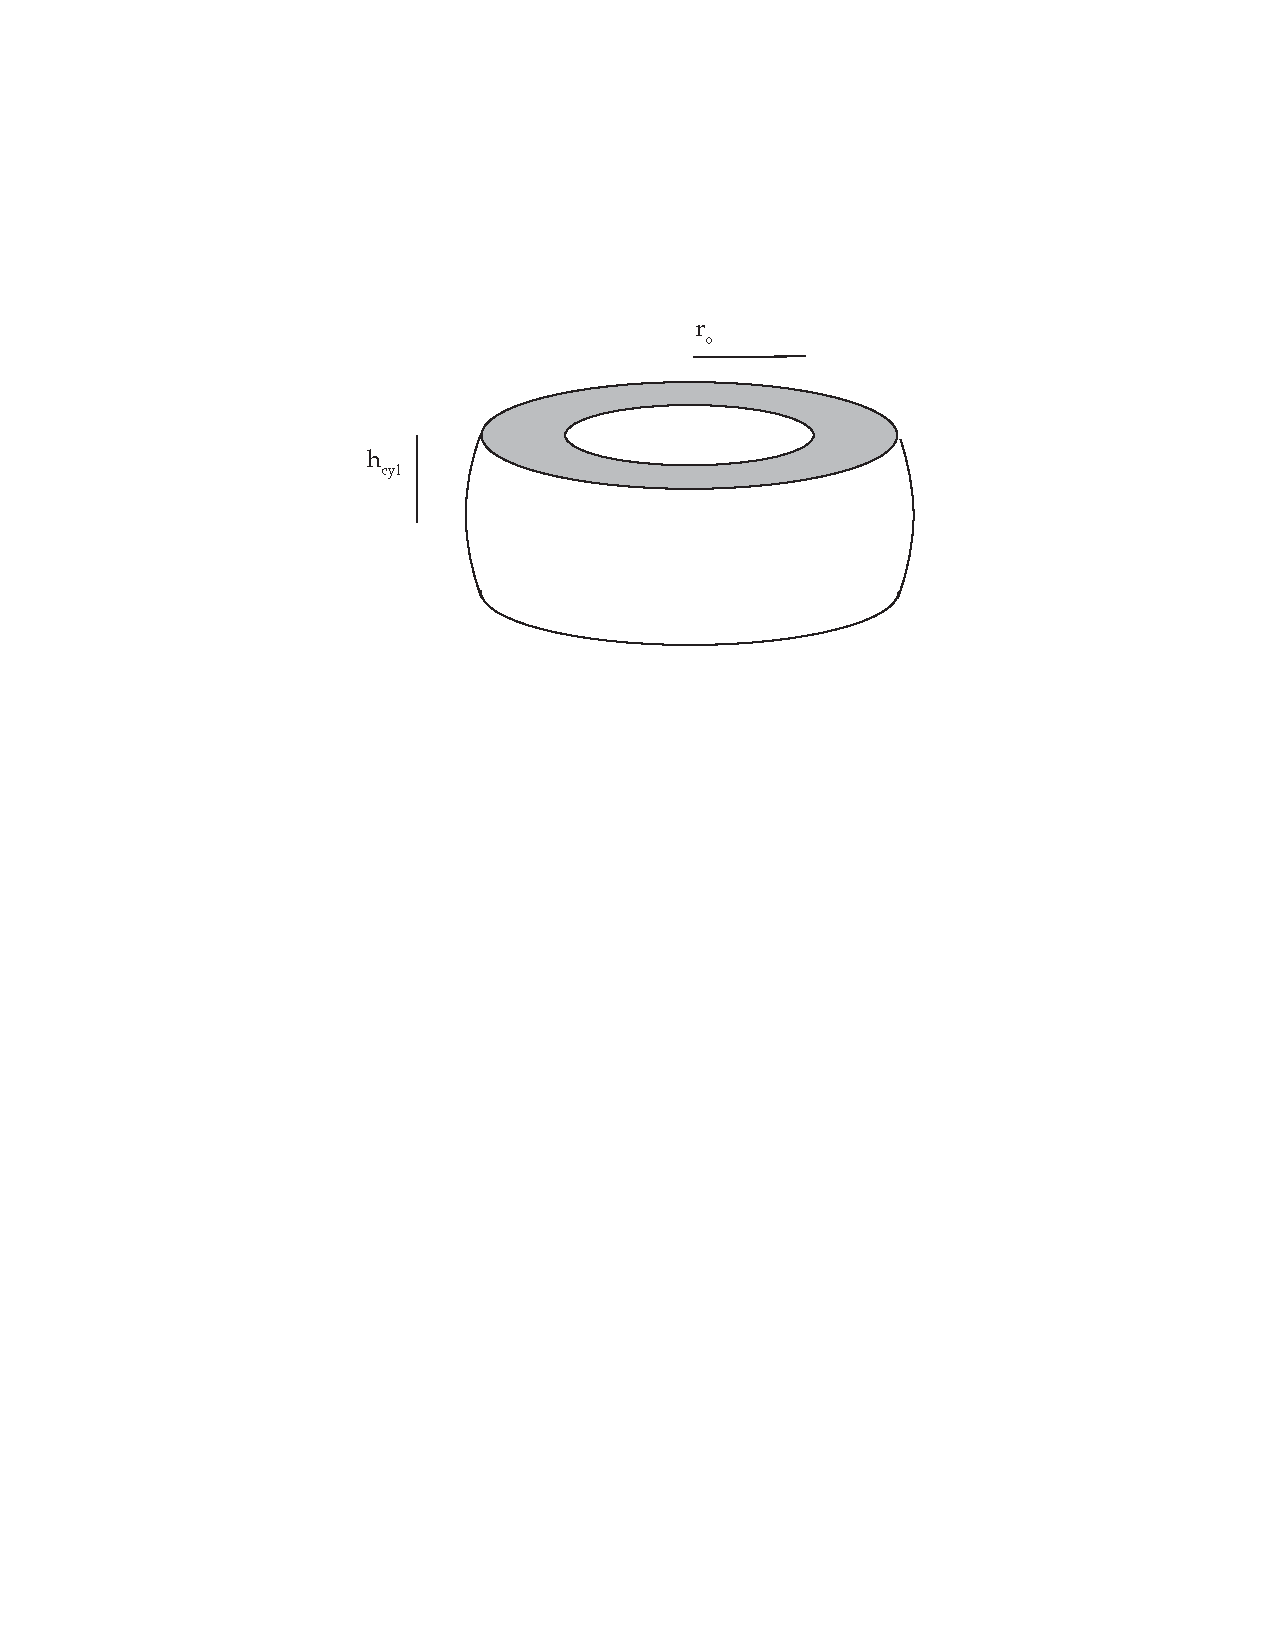
\includegraphics{cylin}
\caption[Cylindrical geometry]
{\label{fig:cylin}This figure shows the geometry assumed when the \cdCommand{cylinder} command
is used.}
\end{figure}

The inner and outer radii of the cylinder are set by
the \cdCommand{radius} command.
The \cdCommand{cylinder} command sets the full height of
the cylinder to twice the number entered on the command.
The argument is
the log of the semi-height in cm.

The effective volume element used to compute the emissivity of the gas
is given by
\begin{equation}
\label{eqn:cylin}
d{\kern 1pt} V = 4{\kern 1pt} \pi \,r_{\mathrm{o}}^2 \left( {\frac{r}{{r_{\mathrm{o}}
}}} \right)\left( {\frac{{\min \left( {r,\;h_{cyl} } \right)}}{{r_{\mathrm{o}}
}}} \right)\;f\left( r \right)\;dr
\,[\mathrm{cm}^{3}]% (45)
\end{equation}
where $r_{\mathrm{o}}$ is the inner radius, $h_{cyl}$ is the cylinder
half-height, and $f(r)$
is the filling factor.
The default value is $h_{cyl}= 10^{35}$~cm.

Changing the emissivity as described by equation \ref{eqn:cylin}
is the only effect of this command.
It does not alter the radiative transfer methods and is
only formally correct when the continua and lines are optically thin.

When combined with the \cdCommand{aperture slit} command, it will be assumed
that the slit is oriented along the rotational axis of the cylinder. If the
slit is oriented at an angle, you can model this geometry by dividing the
height of the cylinder by the cosine of the angle. If the slit is
perpendicular to the rotational axis you can simply omit the cylinder command
since it will have no effect on the predicted spectrum.

\section{Distance 3.2 linear parsecs}

This sets the distance to the object from the Earth.
The number is the
log of the distance in centimeters.
The \cdCommand{linear} keyword forces the number
to be interpreted as the linear distance and the
\cdCommand{parsecs} keyword changes
the units to parsecs.

If the distance is set then it is possible to predict the emission-line
fluxes observed at Earth if the luminosity case is
computed.
If the distance is set with this command then the observed
emission-line fluxes at the Earth will be printed if the
\cdCommand{print line flux}
command is also entered.

This command can be combined with the \cdCommand{aperture} command
to simulate observing parts of a nebula from the Earth.

\section{Filling factor = 0.05 [index =-1]}
\label{sec:CommandFillingFactor}

The first number is the filling factor $f(r)$ for a clumpy model (AGN3
Section 5.9).
It can be either the filling factor itself (which is greater
than zero and less than or equal to one) or the log of the filling factor
(if it is less than or equal to zero).
The second optional number is the
index  for a power-law variation of the filling factor $f(r)$, i.e.,
\begin{equation}
f\left( r \right) = f\left( {r_{\mathrm{o}} } \right)\left( {\frac{r}{{r_{\mathrm{o}}
}}} \right)^\alpha
%(46)
\end{equation}
where $r_{\mathrm{o}}$ is the inner radius of the cloud.

The filling factor is used in two ways.  The first is to modify the volume
emissivity of the gas,
\begin{equation}
dE = \varepsilon \,f\left( r \right)\,\,dV\,\frac{\Omega }{{4\,\pi }}
\,[\mathrm{erg\, s}^{-1}]% (47)
\end{equation}
where $\Omega/4\pi$ is the covering factor.
The second is to modify the optical depth scale
\begin{equation}
d\tau  = \alpha _{l,u} \left( {n_l  - n_u \frac{{g_l }}{{g_u }}}
\right)f\left( r \right)\,dr
%(48)
\end{equation}
(see \citealp{Osterbrock1959}).

A filling factor greater than unity is not allowed.  \Cloudy\ will set
a filling factor of unity if a value greater than one is entered.   The
code will complain (but compute the model) if a filling factor is set in
a constant pressure model since this makes no physical sense.

\section{Illumination angle 45 deg [radians]}

The plane-parallel slab is illuminated by a beam $\theta $
away from the normal.
The default is $\theta  = 0$ (normal illumination).
The angle is in degrees unless
the keyword \cdCommand{radian} appears.

The only effect of this command is to cause the beam of incident radiation
to be attenuated by $\tau n / \cos(\theta )$ where $\tau n$
is the normal optical depth of the zone.
The line and diffuse continua optical depth scale, which is
defined normal to the plane, are not directly affected by this command.

\emph{N.B.}  If this is used with the \cdCommand{grid} or
\cdCommand{vary} options the angle must be given in radians.
See the discussion of the commands with a \cdCommand{vary} option.

\section{Radius r(inner)  [r(outer), thickness; parsec; linear]}
\label{sec:RadiusCommand}

The first number is the log of the inner radius.
The second optional
number sets a stopping radius and is either the log of the
outer radius
(if it is larger than the first number) or the log of the thickness of the
cloud (if it is less than or equal to the first number).

The numbers are normally interpreted as the log of the radii in cm.
If the optional keyword \cdCommand{linear} appears then
the numbers are interpreted
as linear numbers.
The default units are centimeters.
The arguments will
be interpreted as the log of the radii in parsecs if the keyword
\cdCommand{parsec} appears.
Arguments will be interpreted as linear parsecs if both keywords
appear.
The following gives examples of its use.
\begin{verbatim}
radius 19.5       # log of inner radius in cm
radius 19.5 18.5  # as above, but a thickness of 3x10^18 cm
radius 19.5 20    # inner radius as above, outer radius 10^20 cm
radius 100 linear # inner radius of 100 cm
radius 0 parsecs  # log of radius in parses, so inner radius 1 pc
radius 1 to 3 linear parsecs # inner radius 1 pc, outer 3 pc
\end{verbatim}

The default outer radius is effectively infinite (actually $10^{31}$~cm).
If the intensity case is used then a starting radius of $10^{30}$~cm
will be set by default.
Under most circumstances this will result in a
plane-parallel geometry.

Page \pageref{sec:RadiusVaryOptions} describes a problem
that can occur if the second parameter is used with the
\cdCommand{vary} option.
Please read it if you will vary the radius
with the outer radius set.
The \cdCommand{stop thickness} command provides a way to set
a stopping thickness without specifying a starting radius.

\section{Sphere [options]}
\label{sec:CommandSphere}

\Cloudy\ normally assumes an open geometry, i.e.,
that the gas covering factor is small.
The \cdCommand{sphere} command\footnote{The \cdCommand{slit} and \cdCommand{beam}
options were recognized by the \cdCommand{sphere} command before
version 96.  These options were moved to the \cdCommand{aperture} command which was
introduced in version 96.} \footnote{Before version 96 the \cdCommand{sphere} command included an option to change
the covering factor.  The covering factor was removed from the
\cdCommand{sphere}
command.  Only the \cdCommand{covering factor} command changes the covering
factor.} should be included
to change this assumption for a closed geometry,
one where the covering factor of the gas is large and the model spherical.
This command tells \Cloudy\ to take into account ionization by the diffuse
continua and lines produced in the far side of the nebula
(i.e., from beyond the central object), and not to attenuate
the ionizing continuum by pure
scattering opacities, such as electron scattering,
back scattering by grains,
or Rayleigh scattering.

This option should be set when the geometry is spherical and gas nearly
fully covers the continuum source.
It should not be set when the covering
factor is small so that emission from a cloud is unlikely to encounter
another cloud.
This latter case is the default.
In the language of Van
Blerkom and Hummer (1967), \cdCommand{sphere}
causes \Cloudy\ to assume the symmetric
case (their equation 2.14),
rather than the default zero case (their equation
2.13) for diffuse continua.
Here these are referred to as closed and open
geometries, respectively.

Situations can occur where it is not obvious whether or not
\cdCommand{sphere} should
be used.
In this case it would be best to compute models with and without
\cdCommand{sphere} and compare results.
In most cases this will only make a 10--15\%
difference in predicted quantities.

\subsection{Sphere expanding or static}

Two optional keywords,
\cdCommand{expanding} and \cdCommand{static},
determine how line transfer
is handled.
If \cdCommand{expanding} (the default when
\cdCommand{sphere} is entered) is set then
\Cloudy\ assumes that line photons escaping
from the illuminated face of the
cloud are Doppler shifted away from lines of
absorbing material on the far
side of the shell.
This will be the case if the expansion velocity exceeds
the Doppler width by large amounts.
If \cdCommand{static} is set then line photons
do interact on both sides so that even line photons produced at the
illuminated face of the cloud will be strongly trapped by material on the
far side.
$L\alpha $ radiation pressure in the \hplus\ region will probably be
significant if \cdCommand{sphere static} is set and grains are not present.

It is necessary to iterate at least one time when
the \cdCommand{static} option is
used since the total line optical depths are not known on the first
iteration.
All optical depths are determined self-consistently on second
and further iterations.

The specific effects of \cdCommand{sphere} are the following:
The total continuous
optical depths are assumed to be twice the computed optical depths, and
the initial optical depth is half the total.
All diffuse reemission
(bremsstrahlung, free-bound, etc.) is counted in the outward beam
rather than only half.
Scattering opacities are not considered in the attenuation
of the incident radiation field.
When \cdCommand{static} is set, the optical depth
in L$\alpha$ in the inner direction is set to 10$^5$ on the first iteration.
Otherwise it is 10$^{-20}$.
The total optical depths of lines are twice their computed
depth for the static case.
Finally, ionization by lines and continua
produced in the far side of the nebula is included.
At the end of the
iteration all inward optical depths are set to half of the total value
computed from the previous iteration.

\section{Stop depth\dots}

\section{Stop thickness\dots}

The \cdCommand{stop depth} and \cdCommand{stop thickness} commands
provide methods to set the thickness of a cloud without
specifying its radius.
They are described in other sections.






   
\chapter{OPTICAL DEPTHS AND RADIATIVE TRANSFER}
% !TEX root = hazy1.tex

\section{Overview}

Line transfer is relatively unimportant in
low-density clouds such as \hii\ regions
and planetary nebulae.
Radiative transfer can be important in other
environments,
such as nova shells and the broad-line region of active nuclei,
where excited states of hydrogen have significant
populations and subordinate
lines become optically thick.
In other cases grains are present and all
lines can be absorbed by background opacity.
All radiative transfer effects
are included in the treatment of line formation,
including line thermalization,
destruction by background opacities, pumping by the incident continuum,
and escape from the cloud.

It is necessary to iterate upon the solution if emission lines are
optically thick since total optical depths are not known on the first
iteration.
The default is for a single iteration.
This is
often adequate for low-density nebulae such as planetary nebulae or \hii\ regions.
A second iteration is sometimes enough to establish a fairly
accurate line optical depth scale for many resonance transitions.
Further
iterations are usually needed when subordinate lines are also optically
thick.
The \cdCommand{iterate to convergence} command
will iterate until the optical-depth scale is well defined.

Line-radiation pressure cannot be computed accurately until the total
line optical depths are known,
so this quantity is only meaningful after
the first iteration.
\Cloudy\ will stop if the internal radiation pressure
exceeds half of the surface gas pressure in a constant-pressure
model since
such a geometry is unstable unless it is self-gravitating.
The radiation
pressure is not allowed to exceed half the gas pressure on the initial
iterations of a multi-iteration constant-pressure model.
This is to prevent
the calculation from stopping when the optical depth scale is
not yet well converged.

The following sections outline various commands that affect the
radiative transfer.

\section{Case A [options]}

This has the same options as the Case~B command but sets the \la\ optical
depth to a very small value by default.
This does not turn off induced
processes, which are normally ignored when Case A is assumed.
You would
use the \cdCommand{no induced processes} command to do that.

\section{Case~B [tau ly alpha = 9; options]}
\label{sec:CaseBCommand}

This command is used to check the line emission from  hydrogen-like and
helium-like species in the Case~B limit (AGN3 section 4.2).
This command \emph{should
not} be used in any model that is supposed to represent a real physical
environment.
It is intended only to provide an easy way to check predictions
of the code against simple, more limited, calculations.
In particular,
when this is used the Lyman-line optical depths will be made artificially
large.
This may affect the ionization and temperature of the gas.

With no options, this command sets the inward-looking optical depth of
\la\ for all
atoms and ions of the H- and He-like iso-electronic sequences to
$10^5$ so
that even a one-zone model will be close to
Case~B.\footnote{Before version
96 the default optical depth was $10^9$.  This caused
extreme L$\alpha $ behavior in a grain-free \hii\ region.  The lower value is a better
estimate of the physics that occurs in an actual \hii\ region.}
This optical depth does not depend on the abundance of the element, or even
the presence of the species.
The optional number
is the log of the L$\alpha $ optical depth.
One-sided escape probabilities are
used so the total escape probability is simply that for the inward direction.
In keeping with the Case~B approximation the \cdCommand{Case~B} command suppresses
excited-state line optical depths.

{\bf The Hummer option.}
The species include all collisional processes.
Case~B does not define
the population of the ground or first excited state so a true comparison
with Case~B results should have collisions from these levels turned off.
This is done with the Hummer and Storey option (with the key \cdCommand{Hummer}), to allow
comparison with their 1987 and 1995 papers.
Collisions from the ground
and first excited states \emph{are} included if this second option is not specified.
Collisions between levels with $n\ge  3$ \emph{are} included unless the
\cdCommand{database H-like collision off}
or \cdCommand{database He-like collision off} commands are given.  Collisions
between the $2s$ and $2p$ levels are always included unless the
\cdCommand{database H-like collisions l-mixing off} command is given.
Similarly, this option uses the \citet{Percival1978} $n$-changing collisions and the
classical \citet{PengellySeaton1964} theory for $l$-changing collisions.

In the case of the He-like isoelectronic sequence
the \cdCommand{Case~B} command
sets the optical depths in the singlet Lyman lines to a large value.
The
Hummer \& Storey option has no effect on the He-like sequence.

The \cdCommand{no Pdest} option turns off destruction of
Lyman lines by background opacity.

There are several side effects of this command that may after the spectrum
or physical conditions in unexpected ways.
The large L$\alpha $ optical depth will
often result in an especially strong radiation field within this line.
This affects the gas through photoionization of excited metastable states
of H and He and of those elements
with a small enough ionization potential.
The \cdCommand{no photoionization} option on the \cdCommand{Case~B}
command tells the code not to
include photoionization from excited metastable states like the 2s level
of \hO.
But these strong diffuse fields will also strongly affect the level
of ionization of the gas, making the resulting ionization equilibrium a
fiction.
Optically thin gas is actually described by Case C
(\citealp{Ferland1999}, \citealp{LuridianaEtAl09} and
AGN3 Section 11.4) where continuum pumping enhances Balmer lines.
The large
Lyman-line optical depths that result from the \cdCommand{Case~B}
command will prevent
continuum resonant pumping of the atom.  Beware.

\section{Case C [options]}

This has the same options as the Case~B command but sets the
L$\alpha$ optical depth to a very small value by default.
Case C is described by \citet{Ferland1999} and
\citet{LuridianaEtAl09}.

\section{Diffuse fields [outward, OTS]}

This specifies which method is to be used to transfer the diffuse fields,
the emission from gas within the computed structure.
The options are \cdCommand{outward only} and \cdCommand{OTS}.

The \cdCommand{OTS} option takes into account optical depths
in both the inward and outward directions.
The \cdCommand{OTS} option has a \cdCommand{SIMPLE} option which will
do a very simple OTS approximation without taking optical depths into
account.
All diffuse fields with energies capable of ionizing hydrogen
are assumed to do so, and those with smaller energies freely escape.
This is intended as a debugging tool.

If \cdCommand{outward} is chosen then the code will check for a number.
This determines which of the many forms of the outward-only
approximation (\citealp{Tarter1967}) is used.
The default\footnote{OTS was the default in version 86 and before.} is 2.  This is intended for testing the code.

This choice does not strongly affect the predicted emission-line spectrum
but it does change the temperature at the illuminated face of the cloud.

\section{Double optical depths}

On second and later iterations the code uses the total optical depths
of the computed structure to find the outwardly-directed radiation field.
This command doubles the total optical depth so that the shielded face of
the cloud becomes the mid-plane of a structure that is twice as thick as
the computed cloud.

This original purpose of this command was to simulate a geometry in which
ionizing radiation strikes the plane-parallel cloud from both sides.
Examples are a L$\alpha$ forest cloud or the diffuse ISM.
The total line and
continuum optical depths are set to twice the computed optical depth at
the end of the iteration.
The computed model is then one half of the cloud
and the other half of the cloud is assumed to be a mirror image
of the first half.
Doubling the total line and continuum optical depths at the end of
the iteration is the \emph{only} effect of this command.
Physical quantities such
as the physical thickness, column densities, or line emission
\emph{are not} affected.

This approximation makes sense if the cloud is optically thick in lines
but optically thin (or nearly so) in continua.
Lines such as the L$\alpha $
transitions of He I and He II can be important sources
of ionizing radiation.
Their transport will be handled correctly in this limit when this command
is used.
Continuum transport out of the cloud will also be treated
correctly, but attenuation of the incident continuum will
\emph{not} be if the
cloud is optically thick in the continuum.

The second use of this command is when the outer edge of a computed
structure is not the other edge of the cloud.
A typical PDR calculation
is an example.
The calculation starts at the illuminated face and continues
until the gas becomes cool and molecular.  The stopping point often does
not correspond to the outer boundary of the molecular cloud, but rather
is a point that is ``deep enough'' for a given study.  The optical depths
are always computed self-consistently.  On second and later iterations the
total optical depths are normally those of the computed structure.  Near
the shielded face the outward optical depths will be small and radiation
will freely escape in the outward direction.  The gas temperature may fall
dramatically due to the enhanced cooling resulting from the free escape
of line photons.
In real PDRs considerable neutral or molecular material
probably extends beyond the stopping point so that line photons do not freely escape.
The shielding effects of this unmodeled extra material can be
included with this command.
Then, the shielded face of the cloud will
correspond to the mid-plane of the overall structure and lines will not
artificially radiate freely into the outer (unmodeled) hemisphere.

\section{Iterate [2 times, to convergence]}
\label{sec:IterateCommand}

This specifies the number of iterations to be performed.
The default
is a single iteration, a single pass through the model.
At least a second
iteration should be performed in order to establish the correct total optical
depth scale when line transfer or radiation pressure is important.
Two
iterations are sometimes sufficient and will be done if no numbers are
entered on the command line.
A comment will be printed after the last
iteration if the total optical depth scale has not converged and further
iterations are needed.

\subsection{Number of iterations}

There is a slight inconsistency in how the code counts the number of
iterations.
The way it functions in practice is what makes the most sense
to me.

The word \emph{iterate} is from Latin for ``again.''
So the true number of
``agains'' should be one less than the total number of calculations of the
cloud structure.
When the \cdCommand{iterate} command is not entered there is one
calculation of the structure and so formally no iterations.
 If any one
of the following commands is entered:
\begin{verbatim}
iterate
iterate 0
iterate 1
iterate 2
\end{verbatim}
then exactly two calculations of the structure will be done.
If the number
on the line is two or greater, then the number will be the total number
of calculations of the structure.

\subsection{Iterate to convergence [max =7, error =.05, all] }

This is a special form of the \cdCommand{iterate} command
in which the code will
continue to iterate until the optical depths have converged or a limit to
the number of iterations has been reached.
The optional first number on
the line is the maximum number of iterations to perform with a default of
10.  The second optional number is the convergence criterion.
The default
is for relative optical depths to have changed by less than \autocv\ between
the last two iterations.
The optional numbers may be omitted from right
to left.
If all transitions are optically thin then only a second iteration
is performed.

If the \cdCommand{all} option is given, the convergence test will be
made on all transitions, rather than a selected set.

Section \ref{sec:ConvergenceProblems} discusses some reasons the
simulation may not converge.  
There are likely to be convergence problems if the outer edge of the cloud
is set by the lowest allowed temperature rather than an outer radius of column density.

\subsection{Convergence problems}
\label{sec:ConvergenceProblems}

The code generally will not converge if it has not done so within ten
or so iterations.
The most common reason for convergence problems is that
the outer edge of the cloud changes from iteration to iteration.
To prevent this from happening it is important to understand why the
calculation stopped (Section \ref{sec:StoppingCriteria}).

Convergence problems often happen if the outer edge of the cloud is set by
the lowest allowed temperature, as set with the
\cdCommand{stop temperature} command (Section \ref{sec:CommandStopTemperature}),
or the default lowest allowed temperature.
The temperature at the shielded face of the cloud can be affected by the total optical depths.
As a result the point where the lowest temperature is reached can change from
iteration to iteration, so the column densities and optical depths also change,
independently of the radiative transfer solution.
It will not be possible to converge the optical depths since so much is changing.
The code will generate a caution if the solution is not converged after
the limit to the number of iterations is reached.
In that case it will also check if the calculation stopped due to the low-temperature limit
being reached, and suggest changing the stopping criteria in that case.

Another common reason for convergence problems is that
the specified column density or thickness causes the simulation to end
within a prominent ionization front.
In this case very small changes in the
physical conditions result in large changes in the optical depths.  

These
are physical, not numerical, problems.
To prevent them, understand what sets the outer edge of the cloud. 
The code should not have convergence
problems if the outer edge is determined by the outer radius, total column density,
or an equivalent, such as $A_V$.

\section{No scattering opacity}
\label{sec:CommandNoScatteringOpacity}

This turns off several pure scattering opacities.  These include
scattering by grains, electron scattering, and the extreme damping wings
of Lyman lines (Rayleigh scattering).
When scattering opacity is included
and an open geometry is computed the scattering opacity is assumed to
attenuate the incident radiation field as
$\left( {1 + 0.5\,\tau _{scat} } \right)^{ - 1} $
rather than $\exp \left( { - \tau } \right)$ (\citealp{Schuster1905}).

Scattering can be neglected in a spherical geometry with gas fully
covering the source of ionizing radiation.
Scattered photons are not really
lost but continue to diffuse out with (perhaps) a slight shift in energy.
Electron scattering is generally the most important scattering opacity in
a grain-free mixture.
If $ \tau _{scat}  \le 1$
then it is reasonable to consider electron scattering as a heating and
cooling process but not as an absorption mechanism if the energy shifts
are not large (i.e., $ h\nu \ll mc^2$) and the geometry is spherical
(this is not correct for $\gamma$-ray energies,
of course).
\Cloudy\ is not now designed to work in environments that are
quite Compton thick, but should work well for clouds where the electron
scattering optical depths are less than or of order unity.

When this command
is entered scattering processes such as Compton energy exchange 
and grain scattering are still included
as heating, cooling, and ionization processes, but not as extinction sources.
(Thermal and ionization effects of Compton scattering are turned off with
the \cdCommand{no Compton} command).
The \cdCommand{no scattering opacity} command is automatically
generated when \cdCommand{sphere} is specified.

\section{Turbulence = 100 km/s [log, dissipate]}

This enters a microturbulent velocity $u_{turb}$.
The velocity is given in
km s$^{-1}$ on the command line although the code works with
cm s$^{-1}$ internally. The turbulent line width $u_{turb}$ is zero by default,
but the value that is entered must be $u_{turb} \ge 0$.
If the optional keyword \cdCommand{log} appears then the number
is interpreted as the log of the turbulence. Alternatively, you can
also enter the keyword \cdCommand{equipartition} which is discussed
further below.

Turbulent pressure is included in the equation of state when the total
pressure is computed.\footnote{Turbulence was not included as a pressure term in versions 06.02
and before.}
The \cdCommand{no pressure}
option on this command says not to include turbulent pressure in the total
pressure.

Turbulence affects the shielding and pumping of lines.
Fluorescent
excitation of lines becomes increasingly important for larger turbulent
line widths since a larger part of the continuum can be absorbed by a line.
Line pumping is included as a general excitation mechanism for all lines
using the formalism outlined by \citet{Ferland1992} and described further in
a section of Part 3.
The line-center optical depth varies inversely with
the line width velocity $u$ so the effects of line optical depths
and trapping become smaller with increasing line width.
Larger $u$ inhibits self-shielding.

\subsection{Definitions }

The Doppler width of any line that is broadened by both thermal motions
and turbulence that is given by a Gaussian is given by the quadratic sums
of the thermal and turbulent parts,
\begin{equation}
u = \sqrt {u_{th}^2  + u_{turb}^2 }  = b = \sqrt 2 \sigma\;
 [\cmps ].
\end{equation}
Here $b$ is the Doppler parameter used in much of the UV absorption-line
literature, $\sigma $ is the standard deviation
(often called the dispersion) for
a normal distribution, and $\sigma^2$ is the variance.
For a thermal distribution
of motions the average velocity along the line of sight
(\citealp{Mihalas1978}, equation 9-35, page 250)
and the most probable speed (\citealp{Novotny1973}, p 122)
of a particle with mass $m$ are both given~by
\begin{equation}
u_{th}  = \sqrt {2kT/m}\;
[\cmps ].
\end{equation}
This corresponds to $16.3 \sqrt{ t_4/m_{AMU}}\ {\rm km\ s}^{-1}$ for pure thermal motions.
This command sets $u_{turb}$.
Note that with these definitions the full-width half-maximum
(FWHM) of a line is equal to
\begin{equation}
u\left( {FWHM} \right) = u\sqrt {4\ln 2}\;
[\cmps ].
\end{equation}

\subsection{Turbulent pressure}

For an ideal gas the thermal pressure is $P = nkT$
while the energy density is $1/2 nkT$
per degree of freedom, so for a monatomic gas is $U = 3/2 nkT$.
Turbulent motions add pressure and energy terms that are analogous
to thermal motions if the turbulence has a Gaussian distribution.
Note
that the turbulent velocities may be organized, or lined up in certain
directions, if the gas is magnetically controlled.
This presents a
complication that is ignored.

\citet{HeilesTroland2005} discuss both turbulence and magnetic fields.
Their equation 34 gives the turbulent energy density in terms of the
one-dimensional turbulent velocity dispersion $\Delta V_{turb,1D}^2 $
(or standard deviation).
Note that we write velocities in terms of $u$
with the relationship $u^2  = 2\Delta V_{turb,1D}^2 $.
Their energy density can be rewritten as a pressure:
\begin{equation}
\begin{array}{ccl}
 P_{turb}  = \frac{F}{6}\rho \,u_{turb}^2&  =& 3.9 \times 10^{ - 10} F\left(
{\frac{{n_{tot} }}{{10^5 \;{\mathrm{cm}}^{ - 3} }}} \right)\left(
{\frac{{u_{turb} }}{{1\;{\mathrm{km}}\;{\mathrm{s}}^{ - 1} }}} \right)^2 \quad \left[
{{\mathrm{erg\; cm}}^{{\mathrm{ - 3}}} {\mathrm{;\ dyne\; cm}}^{ - 2}} \right] \\
&  =& 2.8 \times 10^6 \,\,F\,\left( {\frac{{n_{tot} }}{{10^5 \;{\mathrm{cm}}^{
- 3} }}} \right)\left( {\frac{{u_{turb} }}{{1\;{\mathrm{km}}\;{\mathrm{s}}^{ - 1}
}}} \right)^2 \quad \left[ {{\mathrm{cm}}^{ - 3} \;{\mathrm{K}}} \right] \\
 \end{array}
\end{equation}
where $n_{tot}$ is the total hydrogen density,
$u_{turb}$ is the turbulent velocity,
and He/H$ = 0.1$ was assumed.
The term $F$ accounts for how the turbulent
velocity field is ordered (\citealp{HeilesTroland2005}, their equation 34).
$F$ is 2 for turbulent velocities that are perpendicular to
the magnetic field
as in Alfven waves and $F$ is 3 for isotropic turbulent motions.
The default
value of $F = 3$ is changed by entering a new value as a second number on
this command line.

\subsection{Energy dissipation}

The \cdCommand{dissipate} option on the \cdCommand{turbulence}
command provides a way in include
conversion of wave energy into heat (see \citealp{BottorffFerland2002}).
When
the option is used a third number, the log of the scale length for the
dissipation in cm, must appear.
Then the turbulent velocity will have the form
\begin{equation}
u_{turb} (r) = u_{turb} (r_{\mathrm{o}} )\exp ( - \Delta r/r_{scale} )\quad
\mathrm{[cm\, s}^{-1}]% (55)
\end{equation}
where $u_{turb}(r_{\mathrm{o}})$ is the turbulence at the illuminated face
and $\Delta r$ is the depth into the cloud.
The wave mechanical energy is assumed to have been
converted into heat with a local heating rate given by
(\citealp{BottorffFerland2002})
\begin{equation}
G(r) = 3.45 \times 10^{ - 28} 2^{ - 3/2} u_{turb}^3 (r) \quad
\mathrm{[erg\, cm}^{-3} \mathrm{s}^{-1}]% (56)
\end{equation}

\subsection{Equipartition turbulent - magnetic pressures }

The \cdCommand{equipartition} option on the \cdCommand{turbulence} command sets the turbulent
velocity to an equipartition between magnetic and
turbulent energy densities.
That is,
\begin{equation}
\label{eqn:MagneticEquipartition}
P_{turb}  = \frac{F}{6}\rho \,u_{turb}^2  = P_{mag}  = \frac{{B^2 }}{{8\pi
}}\, \mathrm{[erg\, cm}^{-3}].% (54)
\end{equation}
The \cdCommand{magnetic field} command sets $B$.
The turbulent
velocity is determined from the magnetic field
assuming equation \ref{eqn:MagneticEquipartition}.
\citet{HeilesCrutcher2005} argue that the correlation between turbulent and
magnetic pressures, while true on average, does not hold in detail for
specific regions of the ISM. When this option is used, you can optionally add
the parameter $F$ on the command line (the default is $F=3$). The keyword \cdCommand{no pressure} is
supported, but not \cdCommand{dissipate}.

\subsection{Turbulence command heads up!}

\emph{N.B.!}  In the default (non-equipartition) form of the command, the turbulent velocity is the first number
on the command line.
The $F$ parameter is the second number.
The energy-dissipation scale length is the third number and must appear
after $u_{turb}$ and $F$.
These numbers can only be omitted from right to left.
In the equipartition case you can only specify $F$,
which then is the first number on the command line.
The energy-dissipation scale length is not supported in the equipartition case.
The keyword \cdCommand{vary} is only supported in the non-equipartition case,
in which case the turbulent velocity is varied.

The turbulent velocity must be less than the speed of light.
The code will stop if $u_{turb} \geq c$ is specified.

\section{vlaw alpha=-1}

This specifies a turbulent velocity that is a power law in radius.
The number is the power law $\alpha$ on radius.
It must be negative.
The turbulence will be given by
\begin{equation}
u = u_0 \left( {{\raise0.7ex\hbox{$r$} \!\mathord{\left/
 {\vphantom {r {r_0 }}}\right.\kern-\nulldelimiterspace}
\!\lower0.7ex\hbox{${r_0 }$}}} \right)^\alpha
\end{equation}
where $r_0$ in the inner radius and
$u_0$ is the initial turbulence specified with the
\cdCommand{turbulence} command.
   
\chapter{THERMAL SOLUTIONS}
% !TEX root = hazy1.tex

\section{Overview}

This Chapter describes options that affect the thermal solution and the
gas kinetic temperature.

The accuracy of the thermal solution is set by the error tolerance in
the heating---cooling balance.
This is set with the \cdCommand{set temperature tolerance} command.
Other commands can change some details of the thermal solution.

\section{cextra -14.231 [temp to the 1.5 power]}

This adds an extra cooling term due to some unspecified physical process.
The first number is the log of the cooling rate [erg cm$^{-3}$~s$^{-1}$].  The second
number is an optional exponent that specifies a temperature dependence.
The cooling will be given by
\begin{equation}
\Lambda  = 10^{c_1 }  \times \left( {\frac{{T_e }}{{10^4 \;{\mathrm{K}}}}}
\right)^{c_2 }
[\mathrm{erg\ cm}^{-3} \mathrm{s}^{-1}]% (57)
\end{equation}
where $c_1$ and $c_2$ are the two numbers entered with this command. If the second
optional argument $c_2$ is not specified then zero
(i.e., constant cooling) is assumed.

The function evaluating \cdCommand{cextra} sets the
variable \cdVariable{cextxx}.
The expression can be easily changed to other forms by changing
how this variable is set.

\section{Constant temperature, t=1e4 K [linear]}

A constant gas kinetic temperature calculation will be performed.
The number
is the electron temperature and is interpreted
as the log
of the value if it is $\le$ 10 or if the keyword \cdCommand{log} is present.
The optional keyword \cdCommand{linear} forces
interpretation as a linear quantity.
The temperature must be within the temperature limits
of the code, currently \TEMPLIMITLOW~$\leq T \leq$~\TEMPLIMITHIGH.

By default the temperature is specified in Kelvin.
The keywords \cdCommand{eV}
and \cdCommand{keV} are also accepted.

Collisional ionization of all atoms and ions is included so this option
can be used to produce clouds in coronal or collisional equilibrium.

\cdTerm{WARNING!}  It is also necessary to specify a
stopping criterion of some
kind when this command is used.
Most thermal-equilibrium calculations stop
when the electron temperature falls below some lowest value, set with the
\cdCommand{stop temperature} command and with the default
value \TEMPSTOPDEFAULT.
This cannot happen with a constant-temperature model.
For
instance, a constant temperature model of a planetary nebula will
continue
until the default limit to the number of zones (now 1400) is reached.
The
\emph{vast} majority of the cloud will consist of predominantly
neutral gas well outside the hydrogen Str\"omgren sphere.
This gas will have a small ambient
level of ionization and emission due to collisional ionization.
The
resulting emission-line spectrum might be surprising since the neutral gas
contributes significant emission.

Any of the stopping criteria described in the
Chapter \cdSectionTitle{Stopping Criteria} can be used.
A more physical constant
temperature model of a ionized cloud could be done by using the
\cdCommand{stop efrac} command to stop the calculation when the hydrogen
ionization front is reached.

\section{Constant grain temperature 20K [linear]}

Normally the temperature of each grain material and size is determined
by balancing heating and cooling.  This command sets the grain temperature
to the indicated quantity.

If the \cdCommand{linear} keyword appears then the number
is interpreted as the linear temperature.
Otherwise numbers $\le 10$ are interpreted as a log
of the temperature.

Other aspects of the grain physics are controlled with the
\cdCommand{grain} command.

\section{Coronal equilibrium, T=1e7 K [linear]}
\label{sec:CommandCoronalEquilibrium}

Coronal equilibrium, in which the gas is collisionally ionized, is
assumed.
The number is interpreted as the log of the
gas kinetic temperature if the
argument is $\le 10$ or the keyword \cdCommand{log} is present, and the linear temperature otherwise.
The optional keyword
\cdCommand{linear} will force the interpretation as a linear temperature.  This holds
the electron temperature at the specified value.

It is necessary\footnote{In versions 87 and before
the \cdCommand{coronal} command set the zone thickness
to 1 cm and stopped after computing one zone.}
to also specify some sort of stopping criteria.
The calculation will probably continue until the default
limit to the number
of zones is reached if a stopping criterion is not specified.
As an example, the following would compute the properties of $1 \pcc$ of a
low density gas at a million degrees Kelvin:
\begin{verbatim}
coronal, T=1e6K
hden 0      # H density 1 cm^-3
set dr 0    # set zone thickness of 1 cm
stop zone 1 # do only one zone
\end{verbatim}

If this is the only energy source specified then it is considered
an intensity command.
Emission-line intensities will be predicted,
as described on page \pageref{sec:IntensityLuminosityCases},
unless a radius is also specified.

Figure \ref{fig:coronal} shows the soft X-ray line and
continuum emission predicted
from the input stream in the test case \cdFilename{ism\_hot\_brems.in}.

\begin{figure}
\centering
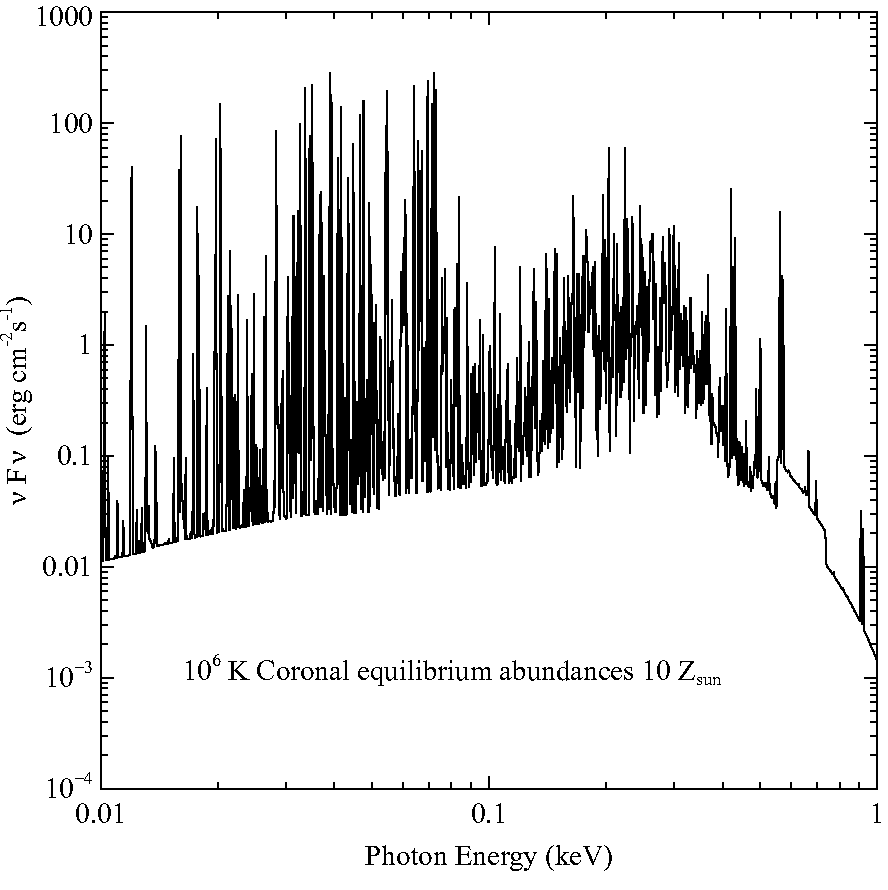
\includegraphics{coronal}
\caption[X-ray emission spectrum]
{\label{fig:coronal}This shows the soft X-ray emission from
the hot phase of a metal-rich ISM in coronal equilibrium.
The input script \cdFilename{ism\_hot\_brems.in} was used
to create the predicted spectrum. }
\end{figure}

The \cdCommand{time init} option provides a way to set initial conditions
for a time-dependent cloud.
This is described beginning on page 
\pageref{sec:TimeVariableRadiationFields}
where the \cdCommand{time} command is discussed.

\section{Cosmic rays [options.\dots]}

This adds cosmic rays and their heating and ionization.  
The command must be specified with at least the first five letters 
to avoid ambiguity with the \cdCommand{cosmology} command.

This physics
is described by \citet{FerlandMushotzky1984},
the subsection \cdSectionTitle{Cosmic Ray Interactions} in the section 
\cdSectionTitle{Other Physical Processes} in Part 3 of this
document, and section 11.3 of AGN3.
Cosmic rays mainly heat ionized gas
and both heat and create secondary ionizations in neutral gas.
All of this
is done self-consistently \citep{Dalgarno1999}.

The \cdCommand{set csupra} command provides a way to
specify an \hO\ secondary ionization rate.
This has many of the same effects
as introducing cosmic rays and uses the same code variables.
The rate
introduced by the \cdCommand{set csupra} command is not
self-consistent with the rest of the calculation but does
provide a way to test the code in certain simple limits.

Cosmic rays must be included if the calculation extends into molecular
regions.
The ion-molecule chemistry that occurs in the cold ISM requires
a source of ionization (\citealp{Dyson1997}).
In fact, most estimates
of the galactic cosmic ray background are based
on the abundances of chemical
ions such as H$_{3}^{+}$ (\citealp{McCall2003}; \citealp{Shaw2008}).
The chemistry
network will probably collapse if the gas becomes molecular
but cosmic rays
are not present.
The code will complain but try to compute the model if
a simulation without cosmic rays extends into cold gas.
If cosmic rays
are not included in the calculation and the neutral hydrogen ionization
rate falls below $10^{-17} \ps$
the code will print a comment stating that the
ionization rate fell below the galactic background rate.

\subsection{Cosmic rays background [1.2]}

This includes galactic background cosmic rays.
We adopt the \citet{Indriolo2007} mean \hO\ cosmic ray ionization rate 
of $2\times 10^{-16} \ps$.
The \htwo\ secondary ionization
rate is then $4.6\times 10^{-16} \ps$,\footnote{Before 2004 the code used a
background ionization rate of $7.4\times 10^{-18} \ps$
quoted by \citet[Table 10]{Tielens1985a}
and \citet{McKee1999}.
The rate of $2.5\times 10^{-17} \ps$ given by \citet{Williams1998} was used through
version C10.}.
(\citet{Glassgold.A74Model-calculations-for-diffuse-molecular} give the
relationship between \hO\ and \htwo\ ionization rates.)
\Cloudy\ determines the heating and
ionization rates of cosmic rays self consistently,
as appropriate for the
local molecular, atomic, and electron densities
(see AGN3 Section 11.3).

An optional scale factor specifies the cosmic ray ionization rate
relative to this background value.
The scale factor is assumed to be a
log unless the keyword \cdCommand{linear} also appears.

The background rate is an active research area.
\citet{McCall2003} find a background rate
$1.2 \times 10^{-15} \ps$ for a galactic
sight line.
\citet{Shaw2008} find a rate about five times larger from detailed
modeling of the sight line to Zeta Per.
\citet{Pellegrini2007} find a significantly enhanced ionization rate in M17.
\citet{Suchkov1993} find cosmic ray ionization rates that are
several dex larger than the galactic background in the starburst galaxy M82. 

The abundance of PAHs (see Section \ref{sec:GrainPAHcommands}) has a
direct effect on the electron density and hence on the cosmic ray seconday
ionization rate of H.  The cosmic ray ionization rate of \htwo\ is nearly twice
the rate for H since two atoms are present.  This command changes the 
atomic hydrogen ionization rate.  
\citet{2021arXiv210103732S} suggest that, for the average Galactic PAH abundance, 
the cosmic ray ionization rate of
atomic hydrogen  is 3.9$\pm$ 1.9\e{-16} \ps.
This rate can be  specified with the command
\begin{verbatim}
cosmic rays background 1.95 linear
\end{verbatim}
\citet{2021arXiv210103732S}  show that the hydrogen cosmic ray ionization rate derived using
H$_3^+$ is much higher, 47.8$\pm$ 23.3\e{-16} \ps,\ if PAHs are not present.

\subsection{Cosmic ray rate -17.3}

If the keyword \cdCommand{rate} appears then the command specifies
the log of the
\hO\ ionization rate [s$^{-1}$] in predominantly neutral gas.
The default is
$2.5\times 10^{-17} \mathrm{s}^{-1}$ taken from \citet{Williams1998}.

\subsection{Cosmic rays density =1.2 [index, etc.]}

If the keyword \cdCommand{density} appears then the first number
is the log of the
cosmic ray density $n(cr)$~[cm$^{-3}$].
Expressions given in \citet{FerlandMushotzky1984} convert this into an ionization rate.

The second optional number is a power-law index $\alpha $ that
describes the
variation of the cosmic ray density with radius, i.e.,
\begin{equation}
n\left( {cr,\;r} \right) = n\left( {cr,\;r_o } \right)\left( {\frac{r}{{r_o
}}} \right)^\alpha
 [\mathrm{cm}^{-3}]  .
\end{equation}
The default value of the index is  $\alpha =0$,
corresponding to a constant cosmic-ray density.
The third optional number is the log of the temperature of
the fast electrons, if they are not relativistic.
If this third number
is specified then expressions from \citet{Balbus1982} will be used
to evaluate the electron heating rates.
The options can be omitted from right to left.

\subsection{Cosmic ray equipartition}

The cosmic rays are assumed to be in equipartition with the magnetic
field.
Then the cosmic-ray density is given by
\begin{equation}
n\left( {cr,\;B} \right) = n\left( {cr,\;B_{_0 } } \right)\left(
{\frac{{U\left( B \right)}}{{U\left( {B_0 } \right)}}} \right)
[\mathrm{cm}^{-3}]%   (59)
\end{equation}
where $U(B)$ and $U(B_0)$ are the energy densities of the local
magnetic field
relative to the galactic background magnetic field.
The \cdCommand{magnetic field}
command sets~$B$.  \citet{Webber1998} gives a cosmic-ray
energy density of 1.8~eV~cm$^{-3}$,
which corresponds to a magnetic field of
$8.5~\mu G$ if equipartition holds.
The background cosmic-ray ionization rate
is scaled by the ratio of the magnetic energy densities to find a local
cosmic ray ionization rate and energy density.

\subsection{The CR background and low-density gas}

The photoelectric heating and radiative cooling of low-density gas varies as the
square of the density while the CR heating varies linearly with density.
This means that CR effects become increasingly important, indeed dominant,
at low enough densities.
Figure \ref{fig:crDensityTemp} shows this.

The figure shows calculations in which both the galactic starlight and cosmic backgrounds 
are included.  
One set of calculations has the full cosmic ray background density while the second
has $10^{-5}$ of that value.  
The two nearly agree at high densities where CRs have little effect.
The effects of the CRs become increasingly dominant at lower densities, causing
the gas to reach temperatures of nearly $10^7$~K at the lowest hydrogen column density shown.

Something to think about before adding cosmic rays to simulations of low-density gas.

\begin{figure}
\centering
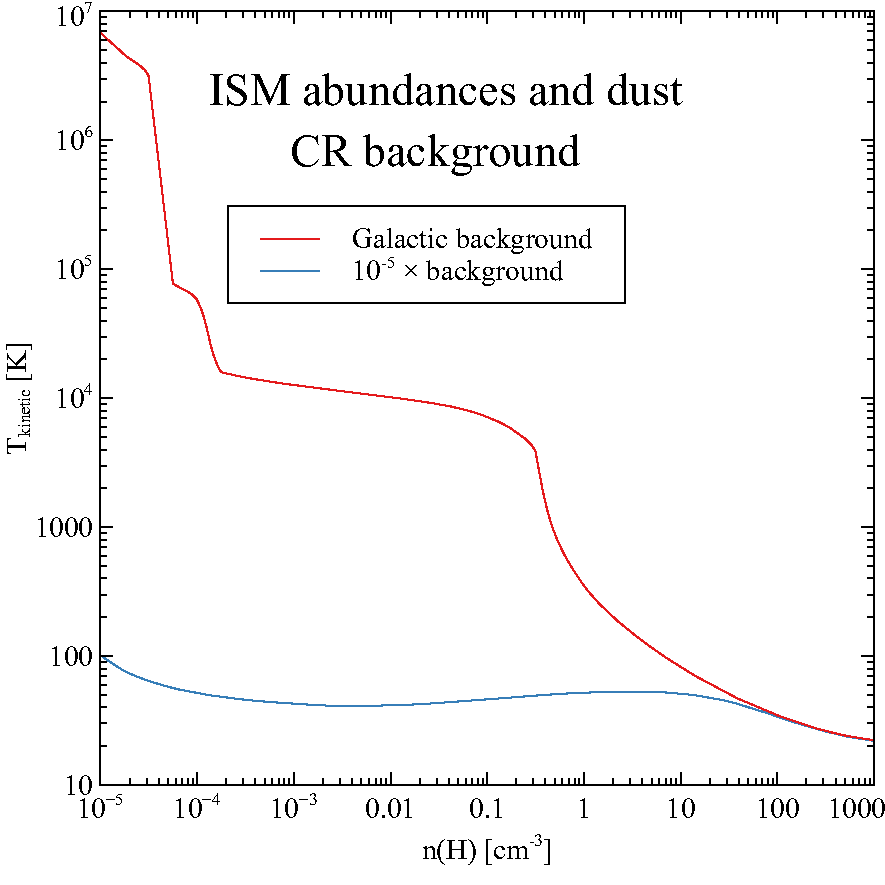
\includegraphics[scale=0.7]{crDensityTemp/crDensityTemp}
\caption[Effects of cosmic ray background on gas temperature]
{\label{fig:crDensityTemp}This shows  
the gas kinetic temperature as a function of hydrogen density for a parcel of ISM gas and dust
exposed to  ISM background starlight and cosmic rays.
The upper curve includes cosmic rays with the galactic background density while
the lower curve has a density $10^5$ times smaller.
The comsic rays strongly affect the conditions in the gas when the hydrogen density is below
$\sim 30 \pcc$.}
\end{figure}


\section{Failures 100 times [ map]}

A converge failure occurs when the heating-cooling balance,
the electron
density, or the pressure, is not within the tolerance set by the
\cdCommand{set convergence} commands.
Normally \Cloudy\ will
punt\footnote{FAQ:  Punt is a technical term from American football.
It is
something bad that happens when progress in advancing the ball is lacking.}
after an excessive number of convergence failures (presently 20)
occur.
This command increases the number of allowed failures to the value
entered as a parameter.

When \Cloudy\ stops because of excessive failures and the
\cdCommand{map} option is
specified\footnote{In versions 94 and before,
the default was to produce the map, and
the \cdCommand{no map} option turned this off.
With version 95 the option is not to
produce a map, and this must be requested with the
\cdCommand{map} option.}
as a keyword on the \cdCommand{failures} command it first
produces a map
of (heating-cooling) versus temperature to give an indication
of where the
equilibrium temperature should have been.
A section in Part 2 describes
thermal failures in more detail and describes this output.

Failures most often occur near a thermal front.
This occurs when the
solution jumps over peaks in the cooling function that occur near
$\sim2000 \K$ and $\sim 10^5 \K$.
A warning will be issued at the end of the calculation if
the global thermal balance is wrong.

It should not be necessary to use this command.
Please post the example
on the discussion board if you find a simulation where you need to
increase the number of convergence failures.

\section{Force temperature to 3400~K}

This forces the initial estimate of the temperature of the first zone
to the value entered.  The temperature is interpreted as a log if it is
$\le 10$ and the linear temperature otherwise.
The keywords \cdCommand{log} and \cdCommand{linear} will override this.

This command is useful if more than one initial temperature solution
is possible.
It forces the first guess of the temperature to the specified
value but \emph{does not} hold the temperature constant.
The temperature is
determined by energy balance thereafter.
(A constant kinetic temperature
is set with the \cdCommand{constant temperature} command.)

\Cloudy\ may have trouble finding a valid first temperature if the initial
solution is forced well away from the equilibrium value.
This is an
inevitable consequence of the complete linearization methods that are
intrinsic to the code's solvers.
If a large number of thermal failures
or warnings result from the use of this command then it is likely that the
code has been forced too far away from the solution.
A better guess of
the initial temperature would fix this problem.

\section{Hextra -14 [depth, density, time, SS]}

This includes extra heating due to some unspecified energy source.
The
first number $H_0$ is the log of the volume-heating rate
[erg~cm$^{-3}\mathrm{s}^{-1}$].
Optional keywords specify how this heating depends on density,
depth into the cloud, or time.
If these optional keywords do not occur then the heating
is constant.

\subsection{Hextra -14 depth 18, thickness 12}

The keyword \cdCommand{depth} makes the heating vary with depth
into the cloud.
The
second number is the log of the scale radius $r_{scale}$~[cm].
The extra heating
rate varies as\footnote{In versions through 94.00 the heating rate
varied as
$\exp[-r_{scale}/(r-r_o)]$ and went to infinity as the illuminated face.  The radial
dependence was changed to its current form in 94.01.}
\begin{equation}
H = H_0 [\exp ( - depth/r_{scale} ) + \exp (T - depth)/r_{scale} )]
 [\ergpccmps ].% (60)
\end{equation}
The third optional parameter $T$ is the total thickness of the slab.
If this
is given then the second exponential term will be added.
This will mimic
an external heat source that warms the cloud from both the illuminated and
shielded faces.
If the third parameter is not entered then the rightmost
term is not included.

\subsection{Hextra -13 density }

The \cdCommand{density} option makes the heating scale with the
hydrogen density.
The heating will be given~by
\begin{equation}
H = H_0 \left[ {n\left( \mathrm{H} \right)/n_0 } \right]
[\ergpccmps ].
\end{equation}
where $n$(H) is the local hydrogen density [cm$^{-3}$]
and $n_0$ is a scale density.
The scale density is unity by default and is changed by specifying the
optional second number, the log of the scale density.

\subsection{Hextra time}

If the \cdCommand{time} keyword appears then the variable
scale factors that appear
on the \cdCommand{time} command will multiply the heating
rate specified with the \cdCommand{hextra} command.
This makes it possible to follow
the effects of time-dependent heating sources.

\subsection{Hextra SS 0.2 1e8 3e17}

When the keyword \cdCommand{SS} appears, the standard $\alpha$-disk model
(\citet{Shakura1973}) will be used. The first parameter is $\alpha$, 
the dimensionless parameter of an $\alpha$-disk model. 
The second number is the mass of center black hole $M$ in solar mass units. 
The last one is the distance [cm] from the center of the disk $r$. 
In this model, heating rate is calculated as
\begin{equation}
H=\alpha P\sqrt{\frac{MG}{r^3}}[\ergpccmps]
\end{equation}
where $P$ is the local gas pressure [erg~cm$^{-3}$] 
and $G$ is gravitational constant. 
All three parameters must appear.
There are spaces to either side of
``\_\cdCommand{SS}\_''. 

\subsection{Notes on the hextra command}

The heating can only depend on depth or density
but the \cdCommand{time} option can
also be specified for each.

By default a calculation will stop when the kinetic temperature falls
below \TEMPSTOPDEFAULT.  It will be necessary to set other stopping criteria such
as the cloud thickness if the extra heating keeps the gas warmer than this
limit.

\section{High temperature approach}

This command tells the code to search for the first temperature by
approaching the thermal solution from the high temperature extreme of $10^6$~K.
Normally the approach is from low temperatures.
This can be useful
when more than one thermal solution is possible.
An example is shown in Figure 10 of \citet{FerlandFabian2009}.

\section{Magnetic field, log(B) = 5 [options]}

Magnetic fields are not included by default.
This specifies the strength
and geometry of the magnetic field.
A number, the log of the magnetic field
strength in Gauss, is the first number on the line.
The physical effects
of magnetic fields are discussed in Part 3 of this document.

Ordered and tangled fields can be specified.
The field is assumed to
be tangled by default.
If the keyword \cdCommand{ordered} appears then the angle between
the radiation field of the central object and the magnetic field
is also specified.
This angle is zero if the field is in the outward radial
direction.
The angle is given in degrees by default but the
\cdCommand{radian} keyword
will cause it to be radians instead.

In the case of a tangled field the code will look for a second number,
the index for the gamma-law relation between the magnetic field and the
gas density.
If a second number is not found then an index of $\gamma = 4/3$,
appropriate for a tangled field, will be assumed.
This index appears in the relationship
\begin{equation}
B_{{\mathrm{tangled}}}  = B_{{\mathrm{tangled}}}^0 \left( {\frac{\rho }{{\rho _0
}}} \right)^{\gamma /2}
 [\mathrm{Gauss}]
\end{equation}
where the term in parenthesis is the ratio of the current density to the
density at the illuminated face of the cloud.
For a spherical
constant-velocity flow, where ${\rho /\rho _0 }\propto(r/r_0 )^{-2} $, the
field will vary as  $B/B_0\propto( r/r_0 )^{-\gamma }$.
This is in contrast with a dipolar field,
in which the radial dependence
is $B/B_0 \propto( r /r_0 )^{-3}$.

Both ordered and tangled fields can be specified on separate commands.
If more than one ordered or tangled field is specified then the second
will take precedence over the first.

The major thermal effect of a field is to add cyclotron cooling.
This is only important at very high temperatures.

Magnetic pressure and enthalpy terms corresponding to the magnetic energy
density are included in the equation of state when a constant-pressure
geometry is assumed.
The magnetic pressure~is
\begin{equation}
P_B /k \approx \frac{{B^2 }}{{8\pi k}} \approx B_{100\,\mu G}^2
\;2.9 \times 10^6 [\pcc \K]
\end{equation}
where $B_{100\,\mu G}$ is
the magnetic field in units of $100\,\mu G$.
The plasma $\beta$ parameter, defined
as the local ratio of thermal to magnetic energy densities,
$\beta  = P_{gas} /P_{mag} $,
is printed in the summary of pressure contributions.
The field affects the dynamics of the gas when $\beta\le 1$.

Supersonic turbulence in rough energy equipartition with the magnetic
field is often observed in the cold ISM (\citealp{HeilesCrutcher2005}).
The
\cdCommand{turbulence} command has an
\cdCommand{equipartition} option
to set the turbulent velocity to a value in energy equipartition
with the magnetic field.
Although a general correlation is observed in the cold
neutral medium of the ISM, it is not thought to be a fundamental relationship (see the Heiles \& Crutcher paper).

\section{Map, zone 4 [range 2000, 5000]}

This computes the heating-cooling vs temperature relation (a ``thermal
map'') of the zone specified as the first number on the line.
This is one
way to check for the existence of more than one thermal solution.
If no
zone is specified, or if the zone is less than or equal to 0, then only
a thermal map is produced for the illuminated face of the cloud and the
calculation then stops.
The calculation of the heating and cooling is
self-consistent across this map.
A section in \cdTerm{Problems} in Part 2 of this
document explains how to interpret the map output.

The map produced by this command is not directly comparable to the more
typical plot that shows the equilibrium temperature as a function of
ionization parameter (\citealp{Krolik1981}).
That map can be
produced by successively calling \Cloudy\ with the same
radiation field
but different densities, say, with the \cdCommand{grid} command.
In that second case each deduced temperature is a valid
equilibrium temperature.
In the map produced by the \cdCommand{map} command only one
temperature, where heating and cooling are equal, is a valid equilibrium
temperature.
The map produced by this command is useful for checking for
more than one thermal solution,
to check that the heating and cooling curves
smoothly flow as the temperature changes,
or to investigate why the code
had convergence problems
(it was originally introduced for only this latter purpose).

The optional keyword \cdCommand{range} specifies the temperature
range of the map.
If this option is specified then the first number on the line must be the
zone for the map, zero if only a map of the illuminated face,
and the next two
numbers must be the lower and upper temperature limits to the map.
These temperatures
will be interpreted as logs if the first temperature is $\le 10$.  Normally
about 20 steps occur between the lowest and highest temperature in the map.
The number of steps can be reset with the \cdCommand{set nmaps} command.

The thermal map can be saved as a separate file with the
\cdCommand{save map} command.
This produces output that is suitable for
processing by other software.

The code stops when the map is complete since it is left in a disturbed
state.

\section{Neutrons -2 [efficiency =-2]}

This adds energy deposition and ionization by secondaries due to the
fast neutrons proposed by \citet{Sikora1989}.
The argument
is the luminosity in fast neutrons expressed as a fraction of the
\emph{total} photon luminosity of the incident continuum.
It is interpreted as a log
if $\le 0$ and a linear scale factor if positive.

The second optional argument is the heating---ionization efficiency
of the neutrons, unity by default.
Both quantities are interpreted as logs
if $\le 0$ and linear if positive.

\section{Print coolants, zone 135}

See the \cdCommand{print \dots} commands below.

\section{Print heating}

See the \cdCommand{print \dots} commands below.

\section{Set temperature [floor, convergence]}

See the \cdCommand{set temperature \dots} commands below.

\section{tlaw [DB96, SN99]}

This specifies a temperature law.
Two options currently are implemented.

The \cdCommand{DB96} option tells the code to use
the temperature---column density
law used by \citet{Draine1996}:
\begin{equation}
T = T_0 /\left[ {1 + N({\mathrm{H}})\,\sigma _{d{,}1000} } \right]
 [\K ]
\end{equation}
where $T_0$ is 500~K and $\sigma$ is $6\times 10^{-22} \pscm$.

The \cdCommand{SN99} option tells the code to use
the temperature - \htwo\ fraction
relationship assumed by \citet{Sternberg1999};
\begin{equation}
T = \frac{{500}}{{1 + 9\left[ {2n\left( {{\mathrm{H}}_2 } \right)/n\left(
{{\mathrm{H}}_{tot} } \right)} \right]^4 }}
 \; [\K].
\end{equation}

\subsection{Tlaw table [depth, radius]}

If the keyword \cdCommand{table} appears on the \cdCommand{tlaw}
command then the code will read
in a set of ordered pairs of radii and temperatures.
There must be two numbers per line
as in the example below.
The first number is the log of the radius or depth
[cm] and is followed by the log of the temperature [K].
If the
keyword \cdCommand{depth} also appears on the command line then
the first number is
interpreted as the log of the depth from the illuminated face
and the table
must begin with a depth smaller than 10$^{-30}$ cm,
the first point where the
depth is evaluated.
The first number is interpreted as the log of the radius
if \cdCommand{depth} does not appear.
The ordered pairs end with a line with the keyword
\cdCommand{end} in columns 1 through~3.

Linear interpolation in log-log space is done.
The following is an example.
\begin{verbatim}
tlaw table depth
continue -35 4
continue 12 4
continue 13 5
continue 14 6
continue 15 7
end of tlaw
\end{verbatim}

Be sure that the first and last radii or depths extend beyond the computed
geometry---this law is only be used for interpolation and the code will
stop if extrapolation is necessary.
Note that the first depth must be
smaller than $10^{-30}$~cm,
and also that there must not be a space in the first
column of any lines with numbers---the code will think that an end of file
has been reached.
Alphabetic characters can be placed anywhere on the line
and will be ignored---I placed the word
\cdCommand{continue} in the first four columns
for this reason (it is actually totally ignored).

      
\chapter{CONTROLLING ATOMIC AND MOLECULAR MODELS}
% !TEX root = hazy1.tex
\label{sec:ControllingAtomicModels}

\section{Species overview}

\Cloudy\ includes models of the internal structure of atoms, ions, and molecules,
which are used to predict line spectra.
We collectively refer to these models as ``species'', as described on page
\pageref{sec:SpeciesDefine} above.
The \cdCommand{database} and \cdCommand{species} commands, described here,
change details of the physical treatment of these 
models.\footnote{The \cdCommand{database} command was the 
\cdCommand{atom} series of commands in C13 and before.  
The code currently accepts \cdCommand{atom} as a
pseudonym for \cdCommand{database}.}  The \cdCommand{database} commands change
properties specific to different atomic and molecular databases, while the \cdCommand{species}
commands change properties specific to an individual atomic or molecular species.

The commands described in this section allow many details concerning the treatment
of a species to be changed. 
For instance, it is possible to change which atomic or molecular database will be used to model a species
and the number of levels to include.

\subsection{How many levels do we include?}
Some models can include many hundreds to thousands of levels.
The strongest lines tend to come from lower levels, although
high levels can be quite important at high densities.
Very large models, with the greatest number of levels, give the best spectroscopic accuracy
but can take quite some time to compute.
By default we include an intermediate number of levels,
chosen as a compromise between execution time and 
an adequate model of the emission and cooling.

\citet{2013MNRAS.429.3133L} describe the logic behind our selection of levels.  
\Cloudy\ can do models in either photo or collisional ionization.
For a particular ion the photoionization case will generally be cooler than the collisional case.
For most elements the default limits are 50 levels for collisional and 15 for photoionization models.  
For iron, which tends to have many more levels due to the number of orbiting electrons,
we settled on a default limit of 100 levels for the collisional case 
and 25 levels for the photoionization case.  

The maximum number of levels for various species can be adjusted with the
commands described in this section.
The actual number of levels computed at a point in the cloud is determined
by the local physical conditions since high levels may not be populated if,
for instance, the temperature is low.

\subsection{Species output options}

\subsubsection{Database print}
This generates a report summarizing properties of all species.
The species label, the number of levels used, and the database
which defined it, are all included.
To see which \Cloudy\ uses by default run this simple test:
\begin{verbatim}
test
database print
\end{verbatim}
The commands described in this section allow changes to the detailed
treatment of each species.

\subsubsection{Save species}
This family of commands, described on 
\pageref{sec:SaveSpecies},
 reports column densities, densities, and other properties
of the species.

\subsubsection{Save lines labels}
In models obtained from external databases, the levels connected by photon
transitions are listed in the output of \cdCommand{save lines labels},
described on \pageref{sec:SaveLineLabels}.

\subsection{The g-bar approximation}

Many transitions do not have collision rates
(collision rates are for more difficult to determine than radiative rates).
We use various forms of the ``g-bar'' approximation,
as originally suggested by 
\citet{Seaton1962} and \citet{VanRegemorter1962},
to fill in missing data.

The \cdCommand{set gbar} (see page \pageref{sec:Setgbar}) controls aspects
of the g-bar approximation.

\subsection{Generating atomic data bibliography}
\label{sec:GeneratingAtomicDataBibliography}

\par
The \cdFilename{scripts/} directory contains tools to generate a summary of 
the references to the original atomic data used by the code.
\cdFilename{db-ref-bib2json.pl} crawls through the database, gathers the
relevant citations, and saves them in a suitable JSON file in the
database directory (e.g., \cdFilename{data/stout/refs.json}).
This file ships with Cloudy, but it may need to be updated.
These citations can be converted to a LaTeX table with
\cdFilename{db-ref-json2tex.pl}.
Currently, only the Stout database is fully supported with these tools.

\par
\cdFilename{db-species-tex.pl} may be used to produce a LaTeX table that
lists the database from which the atomic and molecular data of a
particular run are drawn.
The script operates on the output of the \cdCommand{save species labels}
command, which must be issued in that run.

\par
Please consult the comments at the top of each script for usage instructions
and functional details.


\section{Species ``name'' [options]}

The \cdCommand{species} command provides various options for
controlling behaviour of individual species (atoms, ions or
molecules).  The options are discussed in the following sub-sections.
The species names should be provided in chemical, not spectroscopic,
notation, i.e. \verb|"CO"| or \verb|"O+"|, {\em not}\/ \verb|O 2| or
\verb|"O 2"| -- the species names are case-sensitive.

The parsing of the \cdCommand{species} is stricter than other commands
in \Cloudy, to allow multiple options to be specified at a time.  The
options must be spelt out completely (although they remain
case-insensitive).

\subsection{Species ``name'' off}

This option allows individual {\em molecular}\/ species to be disabled
(i.e.\@ not atoms or ions at present).  This option is useful for
debugging, and investigating the importance of specific species to
chemical pathways.  It should be used with care, as disabling
molecules compromises the physical validity of the model, and may in
some circumstances lead to numerical instability.

\subsection{Species ``name'' levels=[10,all]}

This option allows the number of levels used in modelling
the species to be altered from the default value, within the bounds of
the transition rate data available to \Cloudy.  The command
\begin{verbatim}
species "O+" levels=10
\end{verbatim}
runs a model with 10  levels for the O$^+$ ion, rather than
the default value.  

Using \cdCommand{=all} rather than a numeric
argument requests the maximum available number of levels.
The equal sign is part of the keyword and must be specified with no space
between it and  \cdCommand{all}.

\subsection{Species ``name'' dataset=``abc''}

This option allows you to use an alternate dataset (designated by a nickname)
of atomic or molecular data for a given species. It is only supported for the
Stout database as other databases are developed by third parties and we have a
policy of not altering those databases. The data files belonging to the
alternate dataset are stored in the same directory as the default Stout data
files, but will have a modified filename. For example, if you have a dataset
with the nickname \cdFilename{abc} for species S+2, the full path to the files
will be \cdFilename{data/stout/s/s\_3/s\_3\_abc.nrg}, etc.

Note that the nicknames are case-sensitive as they are part of a filename.
This is why they need to be enclosed in double quotes. See \Hazy~2 for further
details on the datasets that are supported by \Cloudy.

\subsection{Species ``name'' lte}

This option specifies LTE relative populations will be used for the
species, rather than detailed level balance equations.


\section{Database H2 options}
\label{sec:AtomH2}

The large model of the \htwo\ molecule, described in \citet{Shaw2005},
will be included if any of the family of \cdCommand{database H2}
commands appears.
The much
faster three-level model outlined by \citet{Tielens1985a},
\citet{Burton1990}, \citet{Draine1996},
and expanded
by \citet{Elwert2006}, is used by default.
The large molecule is
represented by several thousand levels producing roughly half a million
lines.
AGN3 describes some properties of \htwo\ in section 8.3
and appendix A6.

\emph{NB}  The number ``2'' appears in the keyword for this command.
Any
numerical parameters that appear on the \cdCommand{database H2}
commands must appear after
this two---the code will check that the first number
parsed off the command line is the number~2.

\subsection{The \cdCommand{set H2} command}

Some details of the physical treatment of the \htwo\ molecule can be
changed with the \cdCommand{set H2} command described on page
\pageref{sec:SetH2} below.

\subsection{\htwo\ output options}

Strong \htwo\ lines will appear in the main emission-line output.
The \cdCommand{save H2} command has many other output options.
The
section in Part 2 of this document describing calling the code as a
subroutine describes several routines that will return predictions of the
large molecule.
The \cdCommand{print line precision} command
will add more significant figures to the wavelengths printed in the main
printout.
This may help isolate a particular line.

\subsection{Database H2}

With no options, the only effect is to include the large model of the
\htwo\ molecule.

\subsection{Database H2 chemistry [simple; full]}

This changes how the interactions between the \htwo\ molecule
and the rest of the chemical network are treated.
By default, or if the keyword
\cdCommand{full}
appears, then the fully self-consistent formation and destruction rates
are used when the large \htwo\ molecule is enabled.
If the keyword
\cdCommand{simple} occurs
then expressions from \citet{Tielens1985a} are used instead.

\subsection{Database H2 collisions [options]}
\label{sec:CommandH2CollisionsOptions}

These commands change various collisional processes within
the \htwo\ molecule.

\cdCommand{database H2 ortho para collisions on/off}

This turns off
ortho-para changing
collisions with gas particles.

\cdCommand{database H2 orH2 collisions options}

\cdCommand{database H2 paH2 collisions options}

These commands determine which of the \htwo\ -- \htwo\ collision data
sets is used.
The default is the \citet{LeeH2H22008} set, which can also
be chosen with the \cdCommand{ORNL} option.
The keyword \cdCommand{Le Bourlot} selects the
\citet{LeBourlot1999} data set.
The keyword \cdCommand{ohH2} adjusts the ortho data and the
keyword \cdCommand{paH2} adjusts the para data set.
One of these keywords must be specified.  Both cannot be adjusted
with the same command.

\cdCommand{database H2 H collisions (year)}

This command sets collision rates for \htwo\ -- \hO\ collisions.
There are three data sets.
The default is \cdCommand{2007}, which uses the rates given by \citet{Wrathmall2007}.
The \cdCommand{1999} option uses the rates given by \citet{LeBourlot1999}.   
The \cdCommand{2015} option uses the rates given by \citet{2015MNRAS.453..810L}.
By default we use the \citet{Wrathmall2007} data.

\cdCommand{database H2 He collisions options}

This sets collision rates for \htwo\ - He$^0$ collisions.
There are two data sets.
The default is \cdCommand{ORNL}, which uses the rates given by \citet{LeeH2He2006}.
The \cdCommand{Le Bourlot} option uses the rates given by \citet{LeBourlot1999}.

\cdCommand{database H2 collisional dissociation on/off}
turns on or off collisional dissociation.
The default is to include it using the estimates given in
\citet{Shaw2005}.
These rates are all only guesses and represent an
uncertainty.

\cdCommand{database H2 grain collisions on/off} turns off downward
transitions induced by collisions with grains.

By default the code will uses guesses of collisional rate coefficients
using the g-bar method.
Collisional deexcitation for the g-bar transitions
are turned off with the \cdCommand{database H2 gbar} command.

\subsection{Database H2 gbar [ off; on]}

The g-bar approximation is a rough relationship between the energy of
a line and its collision rate coefficient.  This can be used to guess a
collisional deexcitation rate coefficient when no real data exist.
This command turns this guess off or on.  It is on by default.

\subsection{Database H2 levels }

This changes the number of electronic levels within the \htwo\ molecule.
The default is seven and includes the ground and first six bound singlet
electronic states.
This is also the largest number of levels.  At minimum
is three levels, which is sufficient to include the Lyman and Werner bands
in the UV.
This is the necessary minimum number of levels to include the
correct photodissociation processes.
If no number appears but the keyword
\cdCommand{large} does then the code will use the upper limit.

\subsection{Database H2 limit -4  }

Calculating the level populations and line spectrum of the large \htwo\ molecule is computationally expensive.
The code tries to save time by not
computing the populations when the abundance of \htwo\ is negligible.  This
command changes the limit for the smallest \htwo/H$_{\mathrm{tot}}$ ratio.
The full model
will be computed when the ratio is greater than this limit.
The number
is interpreted as the linear ratio if it is greater than zero and the log
of the ratio if it is less than or equal to zero.
The keyword
\cdCommand{off} turns
off the limit so that the large model of the molecule is always evaluated.
The default limit is 10$^{-8}$, small enough for the large molecule to be
computed across the entire \citet{Tielens1985a} standard PDR
model that is part of the code's test suite.

When the \htwo\ abundance is below this limit the photodissociation,
heating, and cooling rates, are evaluated using expressions in
\citet{Tielens1985a}.
\htwo\ level populations are set to their LTE value so that
self-shielding in the electronic bands is still computed.

\subsection{Database H2 matrix 43}

Populations of the lower ro-vibration states of the ground electronic
level are determined by two schemes.
The first, and most straightforward,
is the solution of a complete set of balance equations by solving
the system
of balance equations with a master equation approach.
The time needed to solve the linear
algebra increases as a power of the number of levels
so we need to keep
the number of levels as small as possible.
High levels are treated by back
substitution, starting from the highest level with X and proceeding
downwards.
This command sets the total number of levels that are computed
within the matrix.
Levels higher than this will be treated with back
substitution.

If the keyword \cdCommand{off} (note the leading space) or
\cdCommand{none} appears, or if the
number of levels is less than 1, the matrix will not be used.
It the keyword
\cdCommand{all} appears then all levels within X will be done this way.

\subsection{Database H2 noise [mean, standard deviation]}

This multiplies the rates for collisional processes within the \htwo\ molecule
by a Gaussian random number so that $r' = r\;10^{{\mathrm{rand}}} $.
Here $r$
is the correct rate coefficient and \cdTerm{rand} is a Gaussian
distributed random number.  There are two optional numbers on the command
line used for generating the Gaussian random numbers.
The first optional number is the mean, with a default of 0.  The second
optional number is the standard deviation with a default of 0.5.

\subsection{Database H2 thermal [simple; full]}

This changes how the heating and cooling by the \htwo\ molecule
are treated.
By default, or if the keyword \cdCommand{full} appears,
then the fully self-consistent
heating and cooling rates are used when the large \htwo\ molecule
is enabled.
If the keyword \cdCommand{simple} occurs then expressions
from \citet{Tielens1985a} are used instead.

\subsection{Database H2 trace [options]}

This turns on trace information concerning the \htwo\ molecule.
The optional
keywords \cdCommand{full}, \cdCommand{iterations},
and \cdCommand{final} will give full information, an overview
of iterations during the convergence, and only final results respectively.
If the keyword \cdCommand{matrix} occurs the code will print
the contents of the matrices
that are used for solution of lower levels within the ground electronic
state.

\subsection{database H2 output options}

Roughly half a million lines are predicted when the large
\htwo\ molecule is included.
The main emission-line printout includes all significant lines
produced in the ground electronic state but does not include electronic
transitions.
The \cdCommand{print line H2 electronic} command
will include these lines.
The family of \cdCommand{save H2} commands
provides ways to save information such as column densities,
the emission-line spectrum, and details of the effects of \htwo\ on the
conditions in the cloud.

%%%%%%%%%%%%%%%%%%%%%%%%%%%%%%%%%%%%%%%
\section{Database H-like \OR{} He-like [element, options]}
\label{sec:atom_H_He_like}

\subsection{Introduction}
These commands are used to change some details in the treatment of atoms of the
H-like and He-like isoelectronic sequences.\footnote{This was the \cdCommand{hydrogenic}
command in versions 90 and before.}
Atoms of the H-like sequence
have one bound electron and include \hO, He$^{+}$, Li$^{+2}$,
through Zn$^{+29}$.
Atoms of the He-like sequence have two bound electrons and include He$^0$,
Li$^+$, through Zn$^{+28}$.

This implementation of the H-like sequence was initially part of Jason
Ferguson's PhD thesis and is described in \citet{FergusonFerland1997},
\citet{Ferguson2001}, and \citet{BottorffBaldwin2002}.
The physics was expanded
to resolve $nl$ terms by Ryan Porter during a visit to IoA
Cambridge in Fall 2008, as was summarized in 
\citet{LuridianaEtAl09}.
Any number of levels up to $n$ of \nHydroMaxLevel\ can be computed.

The He-like sequence was developed by Ryan Porter as part
of his thesis and it is described in \citet{Bauman2005},
\citet{Porter2005},  \citet{PorterFerland2007}, and
\citet{Porter.R12Improved-He-I-emissivities-in-the-case-B-approximation}.
Ryan Porter unified the two sequences
and expanded the H-like sequence to include all of the physics included
in the He-like sequence.

The two sequences are now unified so the same
\cdCommand{database AA-like} commands largely work
for both.

The name of one of the iso-sequences must appear on the command line.  
The options are \cdCommand{H-like} and \cdCommand{He-like}.
Only one iso-sequence can be modified
with a single command.
By default all ions of the iso-sequence are modified.
If the keyword \cdCommand{element} and
the name of an element appears then
only that ion is modified.  
The following are some examples

\begin{verbatim}
# only change hydrogen itself
database H-like element hydrogen resolved levels 8
# change the entire He-like sequence
database He-like resolved levels 9
\end{verbatim}

\subsection{Structure of the model atoms}

The model atoms include a certain number of resolved and collapsed levels
as shown in Figure \ref{fig:LevelsResolvedCollapsed}.
The lower $n_{resolved}$ levels are $nl$ resolved.
Another $n_{collapsed}$ levels,
which replace the $nl$ terms with an $n$ configuration,
are above the resolved levels.

\begin{figure}
\centering
\includegraphics[scale=0.7]{LevelsResolvedCollapsed}
\caption[Resolved and collapsed levels]
{\label{fig:LevelsResolvedCollapsed}This shows  
resolved and collapsed levels for a typical H- or He-like species.
The set of horizontal bars on the left are energy levels with
principal quantum numbers ranging from 1 to 7, increasing from bottom to top.
The lowest three configurations are resolved into $nl$ terms while
higher shells are treated as collapsed levels, in which the $nl$ terms
are assumed to be populated according to their statistical weight.
The levels are adjusted with the \cdCommand{database AA-like levels} command.
This is a cartoon and does not represent any particular species.}
\end{figure}

The physics of the resolved levels is exact while that of the
collapsed levels is more approximate since the entire \emph{n} configuration is
treated as a single level assuming that the $nl$ terms within the \emph{n} configuration 
are populated according to statistical weight.
This is a good assumption at high densities, as
shown by \citet{PengellySeaton1964}.

The total recombination coefficient is the sum to over all possible bound levels.
The model has a finite, often small, number of levels. 
Recombination coefficients to each level are derived from the photoionization cross
section using the Milne relation (AGN3).
The recombination to these levels is less than the total.
We ``topoff'' the model by adding the remaining recombination coefficient
to the model atom, as controlled with the
\cdCommand {database xx-like topoff} command.

By default, the lines produced by the highest levels 
are not included in the printout since their intensities may be unreliable.
The \cdCommand{print line iso collapsed} command,
described in \ref{sec:CommandPrintLineIsoCollapsed},
will cause lines produced by the highest
levels to be included in the printout.
See the discussion of 
the \cdCommand{print line iso collapsed} command for more details.

\subsubsection{The H-like sequence}
Figure \ref{fig:LevelsResolvedCollapsed} shows an H-like system.
Resolved configurations are split into $nl$ levels.
Collapsed levels each represent one principal quantum number.
By default there are \nDefaultResLevelsHlike ~resolved and \nDefaultColLevelsHlike ~collapsed levels for H$^0$ and He$^+$,
and \nDefaultResLevelsHlikeall ~resolved and \nDefaultColLevelsHlikeall ~collapsed levels for heavier elements.

The H-like iso sequence models atoms can extend up to any principle
quantum number between the limits $4 < n \le \nHydroMaxLevel$.
The size is limited mainly
by the available memory and computer time.
Increasing the
number of levels allows a better representation of the collision physics
that occurs within higher levels of the atom at the expense of longer
execution times and greater memory requirements.

\subsubsection{The He-like sequence}

The model atom resolves $n$-levels into $nLS$ levels,
and the 2 $^3P$ term is split into three $nLSJ$ levels.
For a given maximum principal quantum number
$n_{\max}$, there will be a total of $n_{\max}^2 + n_{\max} +1 nLS$ levels.  
The default number of resolved levels for He$^0$ is 6, resulting in
43 $nLS$ levels, 
there are five resolved levels
for C, N, O, Fe, and Zn, and three resolved levels
for all remaining elements.
Increasing $n_{\max}$ allows a better representation of the atom's
emission,
especially the collision physics that occurs within higher levels
of the atom,
but at the expense of longer execution times and greater memory
requirements.

There are also 20 collapsed levels for He$^0$ and one collapsed level for heavier elements.
These collapsed levels
bring together all of the individual $nLS$ terms as one pseudo-level.
The
recombination coefficient into this pseudo-level is the sum of recombination
coefficients into the individual terms plus the recombination topoff.
Transition probabilities from this pseudo-level are calculated as follows.
\begin{equation}
A(n_u \to n_lL_lS)= \frac{\sum_{L_u=L_pm 1} g_{L_{u}S} A(n_uL_uS\to
n_lL_lS)}{\sum_{L_u=L_l\pm 1}}.%49
\end{equation}
This causes the collapsed level to behave exactly as if it were a set of
resolved terms populated according to statistical weight.

There is no limit to the number of levels other than computational resources
like memory and time.

\subsubsection{Selecting  collisional processes}


\cdCommand{database H-like collisions thermal} This option will do the more
precise averaging for all densities, will
be far slower, and should be used when precision is needed. 

\cdCommand{database H-like collisional ionization off}
This command turns off collisional
ionization by thermal electrons of all levels.
Ionization by
cosmic rays is not affected by this command.

\cdCommand{database H-like collisional excitation off}
This command turns off collisional
excitation of all levels, except for 2s-2p.

\cdCommand{database H-like collisions off}
This command turns off collisions for all elements along the H-like
isoelectronic sequence.
All three collisional processes will be turned
off if none of the three keywords are recognized.

\emph{Warning!}  The code will require a very high number of zones
if all collisions
are turned off in an optically thick cloud with a large
$(n \gg 15)$ hydrogen atom.
Collisions will normally hold populations of very highly excited
levels to values very near LTE.
The FIR and radio lines will have very
small line optical depths due to the correction for stimulated emission.
When collisions are absent, the normal tendency of departure coefficients
to increase with principal quantum number means that FIR and radio lines
will strongly mase.
The code dynamically adjusts the zoning to prevent
these maser optical depths from diverging to minus infinity.
A very large
number of zones will be required to spatially resolve the masing region.
This is a totally artificial, not physical, effect.
The solution is to
not turn off collisions with a large atom when performing a
simulation with more than a trivial thickness.


\subsection{Database H-like collisions\dots }
\label{sec:datahlike}

Collisional processes, both between levels and ionization, are controlled
with this command.   This command is mainly
used for testing.  Separate collisional processes can be modified with
the following options.  Only one option is recognized per command line so
multiple commands are needed to turn off several processes.  

\subsubsection{Selecting collisional processes}


\cdCommand{database H-like collisions thermal} This option will do the more
precise averaging for all densities for $n$-changing and $l$-changing
collisional data coming from cross sections. It will
be far slower, and should be used when reference calculations with high
precision is needed.  The default is to use the effective coefficients at $KT$
energy instead of Maxwell averages. 

\cdCommand{database H-like collisional ionization off}
This command turns off collisional
ionization by thermal electrons of all levels.
Ionization by
cosmic rays is not affected by this command.

\cdCommand{database H-like collisional excitation off}
This command turns off collisional
excitation of all levels, except for 2s-2p.

\cdCommand{database H-like collisions off}
This command turns off collisions for all elements along the H-like
isoelectronic sequence.
All three collisional processes will be turned
off if none of the three keywords are recognized.

\emph{Warning!}  The code will require a very high number of zones
if all collisions
are turned off in an optically thick cloud with a large
$(n \gg 15)$ hydrogen atom.
Collisions will normally hold populations of very highly excited
levels to values very near LTE.
The FIR and radio lines will have very
small line optical depths due to the correction for stimulated emission.
When collisions are absent, the normal tendency of departure coefficients
to increase with principal quantum number means that FIR and radio lines
will strongly mase.
The code dynamically adjusts the zoning to prevent
these maser optical depths from diverging to minus infinity.
A very large
number of zones will be required to spatially resolve the masing region.
This is a totally artificial, not physical, effect.
The solution is to
not turn off collisions with a large atom when performing a
simulation with more than a trivial thickness.

\subsubsection{Selecting $n$-changing collision theories}

\citet{Guzman.III.2019} has compared different hight Rydberg collisional excitation 
theories. The commands below select between them.

\cdCommand{database H-like collisions Lebedev} The semiclassical 
straight-trajectory Born approximation from \citet{Lebedevandbeigman1998} is 
used by default. 

\cdCommand{database H-like collisions Vriens} This turns off the default
\citet{Lebedevandbeigman1998} and turns on \cite{Vriens1980} for $n$-changing
collisions.

\cdCommand{database H-like collisions Fujimoto} This turns off the default
\citet{Lebedevandbeigman1998} and turns on \cite{Fujimoto1978} for $n$-changing
collisions.

\cdCommand{database H-like collisions van regemorter} This turns off the default 
\citet{Lebedevandbeigman1998} and turns on \cite{VanRegemorter1962} for $n$-changing 
collisions. 

\subsubsection{Selecting $l$-changing collision theories}

This selects the $l$-changing collision theory.  
As described in \citet{Guzman.I.2016} and \citet{Guzman.II.2017}, we recommend our default option,
the modified  \citet{PengellySeaton1964}, PS-M.

\cdCommand{database H-like collisions l-mixing off}
This turns off all \emph{l}-mixing collisions, including  $2s-2p$.

\cdCommand{database H-like collisions l-mixing Pengelly [Classic]} 
The  modified \citet{PengellySeaton1964} formalism, PS-M, described by 
\citep{Guzman.II.2017}, is used by default.
 If the key \cdCommand{Classic} is used then the original \citet{PengellySeaton1964} is used. 

The \cdCommand{Case B} command, described in Section \ref{sec:CaseBCommand},
uses PS-M by default.
That command has a key \cdCommand{Hummer} to allow comparison with \citet{Hummer1987}, 
that switches to the original \citet{PengellySeaton1964} formalism. This formalism is providing Maxwell averaged rate coefficients so \cdCommand{thermal} option does not apply.


\cdCommand{database H-like collisions [thermal] l-mixing Vrinceanu}  This
changes to the semi-classical formalism  of \citet{Vrinceanu2001}, which reports cross sections.
By default, the rate is derived from the cross section at the most likely collision energy.
Here the density is so low that $l$-changing collisions are unimportant, or so high that the
levels are $l$-mixed. See the \cdCommand{database H-like collisions [thermal]} 
command above for a discussion of the thermal averaging options.


\cdCommand{database H-like collisions l-mixing VOS12 Semiclassical}  This
changes to the approximation shown in equation (9) of \citet{VOS2012}. This formalism is providing Maxwell averaged rate coefficients so \cdCommand{thermal} option does not apply. 

\cdCommand{database H-like collisions  [thermal] l-mixing [thermal] VOS12 Quantal}  This
changes to the approximation shown in equation (2) of \citet{VOS2012}, 
corresponding to a pure quantal treatment of l-mixing collisions.
See the \cdCommand{database H-like collisions [thermal]} 
command above for a discussion of the thermal averaging options.

\subsection{Database He-like collisions \dots.}

This command controls He-like collsional processes. Separate collisional processes can be modified
with these options.
Only one option is recognized per command line
so multiple commands are needed to turn off several processes.
This command modifies collisions for all elements along the He-like
isoelectronic sequence.

\subsubsection{Selecting collisional processes}

As in section \ref{sec:datahlike}:

\cdCommand{database He-like collisions thermal}
%This option will do the more
%precise averaging for all densities for $n$-changing and $l$-changing
%collisional data coming from cross sections. It will
%be far slower, and should be used when reference calculations with high
%precision is needed.  The default is to use the effective coefficients at $KT$
%energy instead of Maxwell averages. 


\cdCommand{database He-like collisional excitation off } 
% This command
%turns off collisional
%excitation, for all $n_u \not= n_l$ transitions,
%for all elements in the helium-like
%isoelectronic sequence.

\cdCommand{database He-like collisional ionization off}
%This command turns off collisional
%ionization by thermal electrons of all levels.

\subsubsection{Selecting $n$-changing collision theories}

The same commands used for H-like explained in section \ref{sec:datahlike} are 
used here.

\cdCommand{database He-like collisions Lebedev} The semiclassical 
straight-trajectory Born approximation from \citet{Lebedevandbeigman1998} is 
used by default. 

\cdCommand{database He-like collisions Vriens} This turns off the default 
\citet{Lebedevandbeigman1998} and turns on \cite{Vriens1980} for $n$-changing 
collisions. 

\cdCommand{database He-like collisions Fujimoto} This turns off the default
\citet{Lebedevandbeigman1998} and turns on \cite{Fujimoto1978} for $n$-changing
collisions.

\cdCommand{database He-like collisions van regemorter} This turns off the default
\citet{Lebedevandbeigman1998} and turns on \cite{VanRegemorter1962} for $n$-changing
collisions.

\subsubsection{Selecting $l$-changing collision theories}

The same commands used for H-like explained in section \ref{sec:datahlike} are {\bf only used for $l>2$}. 
For $l\leq 2$ $l$-shells are highly non degenerate and cannot be adequately treated by $l$-changing theories 
(see \citet{Guzman.II.2017}). 

\cdCommand{database He-like collisions l-mixing [options]} Where as in section \ref{sec:datahlike} 
\cdCommand{options} are  \cdCommand{off}, \cdCommand{Pengelly [Classic]}, 
\cdCommand{[thermal] Vrinceanu} , \cdCommand{VOS2012 Semiclassical} or \cdCommand{[thermal] VOS2012 Quantal}

\cdCommand{database He-like collisions l-mixing all degenerate [options]}  This disables non degenerate calculations 
and all $l-l^\prime$ (also $l\leq2$) collisions are calculated with the model chosen in \cdCommand{options}, 
assuming all the levels are degenerate. This is mainly a testing command. 
The \cdCommand{options} are either \cdCommand{Pengelly}, \cdCommand{Vrinceanu} or \cdCommand{VOS12}.

\cdCommand{database He-like collisions l-mixing [B72|no degeneration] [options]}  
This sets up the criterion for degeneration on collisions. If \cdCommand{B72} is used, 
criteria from equation 3.12 of \citet{1972MNRAS.157..211B} is adopted. 
If \cdCommand{no degeneration}, Pengelly and Seaton \cite{PengellySeaton1964} smoothed 
criteria is followed. If no command, standard calculations, with the criteria used in \citet{Guzman.II.2017}, 
will be performed. The \cdCommand{options} are either \cdCommand{Pengelly}, 
\cdCommand{Vrinceanu} or \cdCommand{VOS12}.

\cdCommand{database He-like collisions l-mixing S62 [off] [degeneration ops] [options]}  
This enables/disables calculations based on \citet{Seaton1962} for $l\leq 2$ where electrons dominate. 
If disabled these values are calculated with the model chosen in the \cdCommand{options}. 
The \cdCommand{options} are either \cdCommand{Pengelly}, \cdCommand{Vrinceanu} or \cdCommand{VOS12}. 
Differently to the \cdCommand{all degenerate} command, {\bf this does not disable non-degenerate $l$-shells}.

\subsection{Database H-like \OR{} He-like  continuum lowering off }
This command disables continuum lowering processes due to particle packing,
Debye shielding, or Stark broadening.  The processes are active by default
and implemented following \citet{Bautista00}.  This command applies
to the entire isoelectronic sequence.

\subsection{Database H-like damping off}

Rayleigh scattering, continuum scattering due to the extreme damping
wings of hydrogen Lyman lines, is turned off with the \cdCommand{damping off} option.
\hi\  Rayleigh scattering is a significant opacity source in clouds that have
large column densities of neutral material
($N$(\hO $) > 10^{23} \mathrm{cm}^{-2}$).

This only disables \hi\ Rayleigh scattering.  
The \cdCommand{He-like} option is not supported. 

\subsection{Database He-like dielectronic recombination [off] }

This option turns dielectronic recombination off for the entire
isoelectronic sequence.
Dielectronic recombination is included by default.
This command only turns off DR.
It affects all elements of the He-like iso sequence.

\subsection{Database H-like \OR{} He-like [element] masers off }

This command turns off masers from collapsed levels for the specified
iso-sequences. Masers are allowed by default for all species. If no 
element is given masers are turned off for all species of that isosequence.

\subsection{Database H-like \OR{} He-like error generation [pessimistic]}

Monte Carlo error analysis can be performed with this command.
Randomly
generated Gaussian errors are applied to atomic data.

The pessimistic option will choose the largest of two standard deviations
for each piece of atomic data.
The full command would look something like
\begin{verbatim}
database He-like error generation pessimistic
\end{verbatim}
Without the
pessimistic keyword the default optimistic values are used.

\subsection{Database He-like gbar options}

The code employs various forms of the $\bar g$
approximation to fill in collision strengths for those transitions with
no quantal calculations.
This command changes which approximation is used.
The options are \cdCommand{Vriens} for the \citet{Vriens1980} and
\cdCommand{off} to set this to zero.
This only exists for the He-like iso sequence.

\subsection{Database H-like \OR{} He-like levels options}

This set of commands controls the model atomic structure shown in 
Figure \ref{fig:LevelsResolvedCollapsed}.

The number of levels can only be set once at the very start of a
calculation when space is allocated for the hydrogenic arrays.
If the code
is used to run a grid of models then only the first occurrence of
\cdCommand{database xx-like levels} is honored and all following occurrences
are ignored.

\subsubsection{Database H-like \OR{} He-like levels resolved \OR{} collapsed  4 [element iron]}

This sets the number of resolved or collapsed levels.
One of the keywords \cdCommand{resolved} or \cdCommand{collapsed} must appear.
The argument gives the principal quantum
number $n$ for the number of levels.
In the case of collapsed levels the number of added levels will be equal to the argument.
In the case of resolved levels a large number of resolved terms may be needed
to produce the requested number of principal quantum numbers.

The following sets most iso sequence models to a small number of levels
but does a high quality simulation of the H- and He- like Fe ions.
\begin{verbatim}
# most ions have small models
database H-like levels small
database He-like levels small
# resolve the lowest n=10 shells, these take well more than 10 levels
database H-like levels element iron resolved levels 10
database He-like levels element iron resolved levels 10
# 15 collapsed levels on top
database H-like levels element iron collapsed levels 15
database He-like levels element iron collapsed levels 15
\end{verbatim}

\subsubsection{Database H-like \OR{} He-like levels LTE}

This will set the level populations to their LTE values.

\subsubsection{Database H-like \OR{} He-like levels print}

This produces a summary of the number of levels for all ions of the iso sequences.
It reports the highest principal quantum number of the resolved levels,
the number of $nls$ terms in these $n$ configurations,
and the number of collapsed levels.

\subsubsection{Setting the number of levels with keywords}

If no numbers occur then we look for a keyword to specify preset sizes.
The code will use the smaller of either the preset size or the current size.

\emph{The H-like iso sequence.}

The keyword
\cdCommand{large} or \cdCommand{small}
specifies either 40 or 5 resolved levels.
Ten collapsed levels are used for the \cdCommand{small} option.

The following would set the full H-like isoelectronic
sequence to a small number of levels, then reset hydrogen, helium,
and iron to a large number.
\begin{verbatim}
database H-like levels small
database H-like levels large element hydrogen
database H-like levels large element helium
database H-like levels large element iron
\end{verbatim}

\emph{The He-like iso sequence.}
If no number appears on the command, but the keyword \cdCommand{large} or
\cdCommand{small} does,
then the number of levels will be large enough to extend
to either $n = 40$ or 3.
Actually, the atoms are
coded so that there is no limit to the number of levels that
can be included, other than the memory and computer time requirements
(which can be substantial for large model atoms).

Use the \cdCommand{database xx-like levels print} to confirm that you are using
the expected number of levels.

{\it A word of caution.} Using a small model atom for He-like species (and
especially for helium itself) can have unexpected consequences. Only the
levels up to $n = 3$ are resolved, meaning that lines coming from higher
levels will be collapsed into one entry with an unusual wavelength. One
particular example for a well-known line is the He\,{\sc i} $1s4d\ ^{3}{\rm D}
\rightarrow 1s2p\ ^{3}{\rm P}^\circ$ triplet line at 4471.49~\AA. This line
will be absent when using a small model atom since it comes from $n = 4$. But
a line at 4469.79~\AA\ will be present, which includes all lines from $n=4$ to
$1s2p\ ^{3}{\rm P}^\circ$. Make sure to study the output of the
\cdCommand{save line labels} command when you are using a small model atom to
understand what the entries on the line stack mean.

\emph{Warning!}  Note that the command
\begin{verbatim}
database H-like levels large
\end{verbatim}
will set all \LIMELM\ hydrogenic atoms to a large number of levels.
This would
require roughly half a gigabyte of memory for the H-like sequence alone,
and would be very slow on today's computers.
It is best to set only the
most important elements to large levels.

\subsection{Database H-like \OR{} He-like Lyman options}

This set of commands changes the treatment of the Lyman lines.
For this purpose, the Lyman lines are all resonance lines,
lines whose lower level is the ground state,  of the  iso sequences.
(Actually, only the \hi\ resonance lines are Lyman lines.)

\subsubsection{Database H-like \OR{} He-like Lyman extra 1000}  

Atoms and ions of the H-like and He-like
isoelectronic sequences use complete multi-level model atoms.
The number of levels included is limited mainly by processor speed and
available memory.
Higher Lyman lines (used here to mean permitted lines that connect directly
to ground) have little impact on emission since they
scatter and are degraded
into Balmer lines and L$\alpha $.
However, an absorption spectrum will show them
as a series of lines converging onto the photoionization continuum from
the ground state.
The code includes a large number of ``extra'' Lyman lines,
included as absorbers with optical depths output with
the \cdCommand{save line optical depth} command,
but not treated as part of the multi-level atoms.
The default number of higher Lyman lines is 100, and
this can be changed to any number with this command.

This changes the number of extra levels for the entire iso-electronic sequence.

\subsubsection{Database H-like Lyman pump}  

These commands control how continuum fluorescent excitation, ``line pumping'', is treated.
They only modify the treatment of \hi\ so the \cdCommand{H-like} keyword must appear.

\subsubsection{Database H-like Lyman pumping off}  
This turns off continuum radiative pumping of the Lyman lines of \hi.
This is one way to take into account the possible
presence of Lyman absorption lines in the incident continuum.

This command is used in the test suite to perform classical PDR
simulations which ignore the \hplus\ region and assume that the PDR is
illuminated by a radiation field with no hydrogen-ionizing radiation.
Classical PDR calculations do not include a full treatment of H or He so
their ions are only produced by cosmic rays.
\Cloudy\ does a full collisional-radiative model
of the physics of \hO\ and \heO\
and will find a thin layer of highly ionized
gas.
This is produced by Lyman-line pumping into excited $np$ levels, some of which decay and
population the metastable $2s$.
That level is then photoionized by relatively low-energy light.
The process stops when the Lyman line optical depths become large enough
for the atom to become self-shielding.
This command will stop this
process from ever becoming important by disabling Lyman line pumping.
(The process would not happen in a realistic calculation
which included the \hplus\ region since Lyman line optical depths
through the \hplus\ region are large.)

This command is included in the ``homework problem'' PDR simulations
in the test suite to
stop Lyman line pumping from occurring.
A better solution would be to include
the PDR as a additional layer outside the \hplus\ region.
The Lyman line
optical depths across the ionized gas in the H~II region will be large and prevent continuum
pumping from occurring in the PDR.
Combining the \hii\ region and PDR also
results in a self-consistent calculation
(\citealp{Abel2005} and \citealp{Abel2008} ).

\subsubsection{Database H-like Lyman pumping scale 3}
The continuum radiative pumping rate
of the Lyman lines of \hi\ will be multiplied by the scale factor
that appears on the line.
This is meant to take into account the possible presence of
Lyman lines in emission or absorption in the incident continuum.
The pumping
rate is normally set by the intensity of the coarse continuum at the line
wavelength.
The number that appears on the command line is a scale factor
that multiplies this continuum.\footnote{In versions C08 and before a value of 0 would produce black Lyman lines.
Starting in C10 values $\le 0$ are interpreted as logs
so a value of 0 will result in a scale factor of unity.}
Numbers $\le 0$ are interpreted as a log and
the \cdCommand{log} keyword will force interpretation as a log.
A value of greater than 1 would correspond to Lyman lines
in emission in the incident radiation field.
A scale factor of 
2 would simulate the presence of stellar Lyman emission lines with peak
intensities twice those of the neighboring continuum.

\subsection{Database H-like \OR{} He-like NO RECOmbination INTErp}

The code normally derives recombination coefficients by interpolating
on a table that lives in the data directory.
This command tells the code
to compute recombination coefficients on the fly by integrating over the
photoionization cross section.

\subsection{Database H-like \OR{} He-like  redistribution [options]}

This changes the form of the redistribution
function for various lines within the model atom.
This command is only
used if you are not happy with the default redistribution functions.
The command changes the redistribution functions for entire iso-sequences.

A keyword to specify which set of lines to change is required.
This is one of \cdCommand{alpha} (the H-like $2p - 1s$ transition or the He-like
$2\, ^1P - 1\, ^1S$ transition)), \cdCommand{resonance} (any higher Lyman line
decaying to the ground term), or \cdCommand{subordinate}
(all Balmer, Paschen, etc lines).
The type of redistribution function to use must also be specified.
The options are \cdCommand{PRD} (partial redistribution), \cdCommand{CRD} (complete redistribution
with Doppler core only), and \cdCommand{CRDW}
(complete redistribution with damping wings).
(The underscore indicates a space.)

The keyword \cdCommand{show} prints the current default
redistribution functions at the time when the command is parsed.

There is at present a fundamental uncertainty in the computation of the
line radiation pressure for transitions such as L$\alpha $.
For a simple two-level
atom with incomplete redistribution, it has long been known that the
line-width is proportional to ($a\tau)^{1/3}$
(\citealp{Adams1972}, \citealp{Harrington1973}; $a$ is
the damping constant).  It is also easily shown that for complete
redistribution and a frequency independent source function that the line
width would be determined by inverting the Voigt function, and hence
proportional to ($a\tau)^{1/2}$.
Line interlocking, whereby scattered Balmer line
radiation broadens the upper level of L$\alpha$
(\citealp{Hubbard1985}), can
alter the line width, as can collisional effects when the density is high
enough for distant collisions to broaden the line.
These effects cause
major differences in radiation pressure and emergent flux (factors of
several) for \la, which can easily have an optical depth of
$10^7$--$10^9$, when
Balmer lines are also optically thick.  
This command determines which
approximation is used.
The default condition is incomplete redistribution,
which minimizes the line width and radiation pressure.  This issue is
discussed further in \citet{Elitzur1986}.

\subsection{Database H-like keep fine structure [ off ]}

The default behavior of \Cloudy\ is to sum all the fine-structure components
of a hydrogenic line together and present them as a single (blended) line on
the line stack. When this command is used, the individual fine structure
components are also pushed onto the line stack. These additional entries will
have a special label to distinguish them from the main hydrogenic line, as is
shown below.

\begin{verbatim}
H  1 s+   6562.81A  -16.989    0.3827
H  1 p-   6562.81A  -16.761    0.6472
H  1 d-   6562.81A  -16.372    1.5858
\end{verbatim}

The extra characters in the label are the $l$ state of the upper level and a
$+$ or $-$ sign indicating whether the $l'$ value for the lower level is
either $l+1$ or $l-1$. So, e.g., \verb=H 1 d- 6562.81A= is the $3d \rightarrow
2p$ transition of hydrogen. If $l > 20$ for the upper level, no character
designation for the quantum number exists and the $l$ value itself will be
printed, e.g., \verb=H 1 22-=. Note that only fine-structure components for
resolved to resolved transitions will be saved, and not for collapsed to
resolved transitions. If the optional keyword \cdCommand{off} is entered,
saving the fine-structure components will be disabled, which is also the
default. This command can only be used for the H-like iso sequence.

\subsection{Database H-like \OR{} He-like topoff [ off ]} 

Atoms have a very large number of levels at low densities.
This model has a finite number of levels, often far smaller than
the number of levels present.
We introduce ``topoff''; to maintain the correct total recombination coefficient and
allow for the proper collisional coupling of the highest levels to the continuum.

This command turns topoff off or on.
The default is to include topoff and the keyword \cdCommand{off} disables it.
This changes the treatment for the entire iso-sequence.

Topoff is necessary to obtain the correct total
radiative recombination rate coefficient with a finite number of levels.
Because only a finite number of levels can be computed the sum
of the total
recombination coefficient will be less than the sum to infinity.
This difference must be added somewhere to conserve the
total recombination rate.  
Similarly, the very highest physical levels should be coupled to the continuum by
collisional ionization / three-body recombination.
When topoff is included the collisional ionization rate for the highest level is increased
by a large factor to mimic the effects of much higher levels 
(three body recombination is obtained from this by detailed balance).

At high densities the continuum is lowered by pressure effects.  If the continuum
is lowered to include levels in the model atom then topoff is not done.
In this case topoff is not needed since we have a complete model of the atom.

\section{Overview to the Chianti, Lamda, and Stout databases}

Three databases, described below, are used by \Cloudy\
to model line emission from atoms and molecules.
Stout is the database we developed for \Cloudy.
\href{http://www.chiantidatabase.org/}{Chianti}  
(\cite{Dere.K97CHIANTI---an-atomic-database-for-emission}; \cite{Landi2012})
was developed to study outer layers of the sun.
LAMDA, the Leiden Atomic and Molecular
Database (\href{http://www.strw.leidenuniv.nl/~moldata/}{www.strw.leidenuniv.nl/~moldata/}, 
\citet{Schoier.F05An-atomic-and-molecular-database-for-analysis}),
contains many molecules.

The following sections document how we use these databases.
Similar options are available for all three.
Our ``species'', how we specify atoms, ions, and molecules,
and their lines, is discussed on \pageref{sec:SpeciesDefine}.

\begin{itemize}
  
  \item Each database has a masterlist file, located in 
  \cdCommand{data/DATABASE}, that lists the species
  to be used with that database.  

  \item If a species is
  present in more than one database the higher priority database is used.
  The Stout database has the highest priority, followed by Chianti and LAMDA.  
  
  \item You can create your own masterlist file
  to cherry pick the species and database you want with the
  \cdCommand{database DATABASE masterlist} command.
  
  \item In general, we use only a fraction of the levels available in the
  database.  The \cdCommand{print} option on the commands
  will report the species and number of levels for that database.
  
  \item The \cdCommand{levels max} option will use all available levels
  for a particular database.
  The calculation will take significantly more time.
  \citet{2013MNRAS.429.3133L} discusses
  the strategy we use to limit the number of levels.
  
  \item It is possible to specify the minimum number of levels 
  for a particular species by entering
  a number following the species name in the masterlist file for Chianti and Stout.
  
\end{itemize}

%%%%%%%%%%%%%%%%%%%%%%%%%%%%%%%%%%%
\section{Database Lamda [on , off][print][levels \{j, MAX\}]}
\label{sec:SetLamda}
The command controls the use of the molecular models from Lamda, the Leiden Atomic and Molecular
Database (\href{http://www.strw.leidenuniv.nl/~moldata/}{www.strw.leidenuniv.nl/~moldata/}, 
\citet{Schoier.F05An-atomic-and-molecular-database-for-analysis}).   
Note that some molecules in LAMDA are not
currently known to \Cloudy 's chemistry.  \Cloudy\ therefore has no means by
which to predict the abundance of those molecules.  In such cases, the
LAMDA models are simply ignored. 

The \cdCommand{database Chianti} command, described on page \pageref{sec:SetChianti},
and the \cdCommand{database Stout} command, described on page \pageref{sec:SetStout},
do similar work for the Chianti and Lamda databases.

%%%%%%%%%%%%%%%%%%%%%%%%%%%%%%%%%%%%%%%%%%%%%%
\subsection{Database Lamda [on off]} 
This will enable or disable the use of the Lamda database.
It is on by default.

\subsection{Database Lamda \cdFilename{"masterlist.ini"}}
The species included in the file \cdFilename{filename}, given between quotes, will be used
instead of the list in the default location in the \cdFilename{data} directory.
The masterlist file must begin with the magic number used in our default masterlist files.
By default we use species listed in the \cdFilename{Lamda.ini} file in the 
\cdFilename{data/lamda/masterlist} directory.
This makes it possible to create \cdFilename{ini} files that select portions of Lamda.

\subsection{Database Lamda print} 
This prints a report giving which Lamda species are being used
along with the number of levels.

\subsection{Database Lamda Levels n} 
This sets the maximum number of Lamda energy levels. 
By default we limit the number of energy levels for Lamda species to 
\nDefaultMolLevels\ .
The \cdCommand{levels} option will overwrite this limit.
The number, $n$, is the level limit.
If no numbers appear but the keyword \cdCommand{MAX} does, we use all 
of the available energy levels.

The \cdCommand{database  Chianti} command, described on page \pageref{sec:SetChianti},
and the \cdCommand{database  Stout} command, described on page \pageref{sec:SetStout},
do similar work for the Chianti and Stout databases.

%%%%%%%%%%%%%%%%%%%%%%%%%%%%%%%%%%%%%%%%%%%%%%
\section{Database Chianti [ options ]}
\label{sec:SetChianti}

This controls the use of the 
\href{http://www.chiantidatabase.org/}{Chianti} database 
(\cite{Dere.K97CHIANTI---an-atomic-database-for-emission}; \cite{Landi2012}).
The \cdCommand{database Lamda} command, described on page \pageref{sec:SetLamda},
and the \cdCommand{database Stout} command, described on page \pageref{sec:SetStout},
do similar work for the Lamda and Stout databases.

The \cdCommand{save chianti} command described on 
page \pageref{sec:CommandSaveChianti} can be used to export parts of 
the Chianti data.

The Chianti database does not contain collision strengths for subordinate transitions.
By default, \Cloudy\ will use the gbar approximation to estimate collision strengths for allowed transitions that do not have data. 
The \cdCommand{Set Gbar} command controls the use of gbar in Chianti and is described on page \pageref{sec:Setgbar}.

The database contains both experimental and theoretical energies.  By default
we use only experimental energies, although this can be changed with the 
\cdCommand{Set Chianti Experimental} command described on page \pageref{sec:AtomChiantiExperimental}.

By default we limit the number of energy levels for Chianti iron species to 
\nDefaultPhotoLevelsFe\ and all other elements to \nDefaultPhotoLevels.
This can be changed with the \cdCommand{Database Chianti Levels}  command
described on page \pageref{sec:AtomChiantiLevels}.

\subsection{Database Chianti \cdFilename{"masterlist.ini"}}
By default, \Cloudy\ uses selected Chianti species between phosphorus and zinc, 
specifically including Fe VI through Fe XXIV.
These species are listed in the \cdFilename{CloudyChianti.ini} masterlist file in the 
\cdFilename{data/chianti/masterlist} directory.
Files in that directory give other sets of species.

If a double quote appears on the line then the filename
between the pair of double quotes will be used instead of
the \cdFilename{CloudyChianti.ini} file.
This makes it possible to create masterlist files that select portions
of Chianti.

\subsection{Database Chianti off} 
will disable all of Chianti.

\subsection{Database Chianti hybrid} 
Hybrid, the merging of the Chianti data with the Opacity Project data, 
is on by default if Chianti is on.
The \cdCommand{no hybrid} option disables the Opacity Project data and only uses Chianti.
See \citet{2013MNRAS.429.3133L} for more details.

\subsection{Database Chianti print} 
will print which Chianti ions are being used
along with the number of levels.
 
\subsection{Database Chianti Levels} 
\label{sec:AtomChiantiLevels}
This sets the maximum number of Chianti energy levels. 
Some ions have a very large number of levels.
These have a significant impact
on the execution time but produce only weak lines and have a minor effect
on the cooling for photoionized clouds.
By default we limit the number of energy levels for Chianti iron species to 
\nDefaultPhotoLevelsFe\ and all other elements to \nDefaultPhotoLevels.
Plasmas in collisional equilibrium tend to be hotter, for a given
stage of ionization, than a photoionized plasma.  
The \cdCommand{Coronal} command, described on
page \pageref{sec:CommandCoronalEquilibrium}, is used for
the collisional ionization case.
The limits to the number of levels are then \nDefaultCollLevelsFe\ for iron 
and \nDefaultCollLevels\ for all others.
The \cdCommand{levels} option will overwrite these limits.
The first number, i, is the iron level limit, while the second number, 
j, is for all other Chianti elements.
If no numbers appear but the keyword \cdCommand{MAX} does, we use all 
of the available energy levels.
See \citet{2013MNRAS.429.3133L} for more details.

\subsection{Database Chianti [experimental theoretical]}
\label{sec:AtomChiantiExperimental}
By default we use experimental Chianti energies.
The \cdCommand{theoretical} option causes \Cloudy\ to only use theoretical 
energies.
This provides significantly more levels and transitions, 
however the error in wavelength is larger.

\section{Database Stout [on , off, no hybrid][print][levels \{j, MAX\}]}
\label{sec:SetStout}
The command controls the use of the Stout database.
The \cdCommand{database Chianti} command, described on page \pageref{sec:SetChianti},
and the \cdCommand{database Lamda} command, described on page \pageref{sec:SetLamda},
do similar work for the Chianti and Lamda databases.

\subsection{Database Stout [on off]} 
command will enable or disable the use of the Stout database.
It is on by default.

\subsection{Database Stout \cdFilename{"masterlist.ini"}}
The species included in the file \cdFilename{filename}, given between quotes, will be used
instead of the list in the default location in the \cdFilename{data} directory.
The masterlist file must begin with the magic number used in our default masterlist files.
By default we use species listed in the \cdFilename{Stout.ini} file in the 
\cdFilename{data/stout/masterlist} directory.
This makes it possible to create \cdFilename{ini} files that select portions of Stout.

\subsection{Database Stout hybrid} 
Hybrid, the merging of the Stout data with the Opacity Project data, 
is on by default.
The \cdCommand{no hybrid} option disables the Opacity Project data 
and only uses Stout.

\subsection{Database Stout print} 
will print which Stout species are being used
along with the number of levels.

\subsection{Database Stout Levels nFe, nOther} 
This sets the maximum number of Stout energy levels. 
Some ions have a very large number of levels.
These have a significant impact
on the execution time but produce only weak lines and have a minor effect
on the cooling for photoionized clouds.
By default we limit the number of energy levels for Stout iron species to 
\nDefaultPhotoLevelsFe\ and all other elements to \nDefaultPhotoLevels.
Plasmas in collisional equilibrium tend to be hotter, for a given
stage of ionization, than a photoionized plasma.  
The \cdCommand{Coronal} command, described on
page \pageref{sec:CommandCoronalEquilibrium}, is used for
the collisional ionization case.
The limits to the number of levels are then \nDefaultCollLevelsFe\ for iron 
and \nDefaultCollLevels\ for all others.
The \cdCommand{levels} option will overwrite these limits.
The first number is the iron level limit, while the second number 
is for all other Stout elements.
If no numbers appear but the keyword \cdCommand{MAX} does, we use all 
of the available energy levels.

      
\chapter{CONTROLLING CHEMICAL MODELS}
% !TEX root = hazy1.tex

\section{The Chemistry command}

Several chemistry sub-commands can be specified on a single line,
separated by commas, e.g.

\cdCommand{chemistry reaction ``$\mathbf{S+,Mg=>S,Mg+}$'' off, reaction ``$\mathbf{S+,Fe=>S,Fe+}$'' off}

\subsection{Chemistry reaction}

The keyword \cdCommand{reaction} takes a string argument for the
reaction which is being referred to.  Care is taken to ensure that the
effect of this command does not depend on the order in which reactants
or products are specified.

At present, it has a single option, \cdCommand{off}, which disables
the reaction.

A list of reactions can be specified for the command, i.e.

\cdCommand{chemistry reaction (``$\mathbf{S+,Mg=>S,Mg+}$'', ``$\mathbf{S+,Fe=>S,Fe+}$'') off}

The brackets, and commas between entries, are required.
      
\chapter{DYNAMICAL \& TIME-DEPENDENT CALCULATIONS}
% !TEX root = hazy1.tex
\label{sec:DynamicalTimeDependent}

\section{Overview}

This section describes the dynamical and time-dependent calculations
that can be done with the code.
This physics was developed in collaboration
with Robin Williams and Will Henney, and \citet{Henney2005}
and \citet{Henney2007} describe first applications.

These calculations begin by doing several iterations to compute the static
structure.
This establishes the optical depth scale that is used in later
calculations.
The number of static calculations is 3 by default and is
reset with the \cdCommand{set dynamics relax} command.

Advective terms are included in the balance equations by adding
upstream quantities that are taken from the previous iteration.
Problems would arise if we needed to look upstream beyond the
outer edge of the computed radial grid.
To prevent this the outer radius found in the static iterations will
be the outer radius of later calculations.
This overrides the behavior of the \cdCommand{radius} command.

\cdTerm{Warning!}  The physics
behind these commands is still being developed.
The heuristics that are needed to control changes in the time steps or the
advancing upstream parameters are not complete.  Output options to capture
the information in the flow or over time are not complete.
All of this is an area of active development.

In the following discussion commands that are still under development are
introduced by the \experimental\ symbol and are in a grey box.

\begin{shaded}
\section{\experimental cosmology }
This follows the time dependent recombination of the early universe.
It was added by Ryan Porter.
It has several options.

\subsection{\experimental cosmology omega}
This specifies an omega parameter.
It accepts the keywords \cdCommand{baryon}, \cdCommand{radiation},
\cdCommand{matter}, \cdCommand{lambda}, and \cdCommand{K}.

\subsection{\experimental cosmology Hubble}
This specifies the Hubble constant in units of
100 \kmpspMpc.
\end{shaded}

\section{A cooling or heating non-equilibrium gas}
\label{sec:Cooling-Heating-NonEq}

This case is a non-equilibrium gas that cools down or heats up
after an initial state is established.
The usual case is a grain-free gas which is not exposed to
an external radiation field.
A unspecified process has established the gas in an equilibrium
state, and the gas is allowed to freely cool or heat.
Recent papers which studied this case are
\citet{Chatzikos2015} and \citet{GnatSternberg07}.

This calculation is set up by doing a coronal equilibrium
calculation with the \cdCommand{coronal 1e4 K init time} command
described on page \pageref{sec:CommandCoronalEquilibrium}.
This establishes an equilibrium collisionally ionized
gas by doing a number of iterations with the kinetic temperature
held fixed at the specified value.
By default the number of iterations is 3, but may be changed
with the command \cdCommand{set dynamics relax [niter]}.

The initial timestep is by default set to a small fraction
($10^{-4}$) of the cooling time, while subsequent timesteps
are set to 4\% of the cooling time.

The \cdCommand{iterate} command tells the code to evolve
the system until some stopping criterion is met.
The command \cdCommand{stop time when temperature below [value]}
tells the code to stop when the lowest temperature falls
below the specified value.

As an example, the following input script evolves a parcel of gas
as it cools isobarically from X-ray temperatures.
The emitted X-ray spectrum is shown in Figure~\ref{fig:coolingFlow}.
%
\begin{verbatim}
coronal 11.654e6 K init time
hden 0.1 linear
constant gas pressure reset
set dr 0
set nend 1
stop zone 1
iterate 300
stop time when temperature falls below 1e4 K
cosmic rays background
#
# commands controlling output    =========
set cumulative mass
set trimming off
set save prefix "cp-cool-1keV"
save time dependent   ".tim"  no hash
save continuum units Angstroms ".concum" cumulative
\end{verbatim}

\begin{figure}
	\centering
	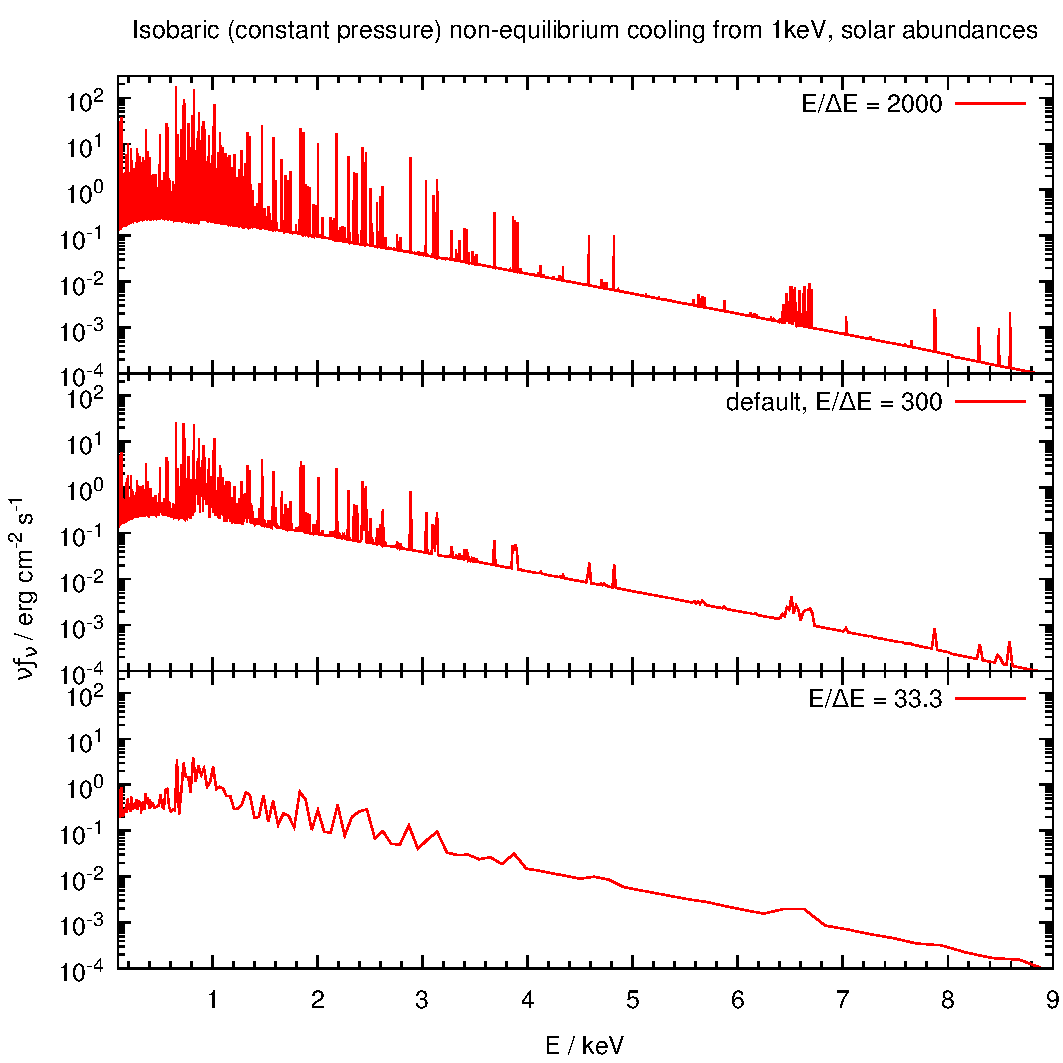
\includegraphics[scale=0.9]{cooling-flow-spectrum-hazy1}
	\caption[Cooling flow]
	{	\label{fig:coolingFlow}
		The X-ray spectrum of a unit-volume parcel of gas cooling under conditions
		of constant pressure (isobarically) from X-ray temperatures (1~keV), computed
		at three resolving powers.
		In the top panel, the resolving power is comparable the proposed {\it Athena}
		resolving power around 6~keV.
		In the bottom panel, the resolving power is comparable to the {\it Chandra}
		non-dispersive resolving power around 1~keV.
		In the middle panel, the resolving power is at the code default.
		This functionality is described in \citet{Chatzikos2015}.
	}
\end{figure}


\begin{shaded}
\section{\protect\experimental Time-variable incident radiation field}
\label{sec:TimeVariableRadiationFields}

This follows the time-dependent evolution of a cloud near a variable
continuum or heat source.

Time-dependent calculations are done by setting up an initial geometry
using the usual commands that specify a cloud and
the incident radiation field.
The \cdCommand{time} keyword establishes which energy sources
vary with time.
The keyword can appear on any of the commands that specify the
luminosity of the radiation field and
on the \cdCommand{hextra} command.
The \cdCommand{trace} option will turn on trace printout.

If a \cdCommand{time} command also occurs
then all radiative and heat sources with
the \cdCommand{time} keyword will change with time.
The \cdCommand{time} command sets a time step
and stopping time.
Each iteration is a time step and the number of time
steps is set with the \cdCommand{iterate} command.
The calculation will stop when
either the number of iterations or the stopping time is reached.

\subsection{time command}

The first argument on the \cdCommand{time} command
is the log of the initial time step in seconds.
The calculation starts at time zero and
the first time step will be this long.
Later time steps will
have their size adjusted by the rate of change in conditions in the gas.
The optional second number gives the log of the stopping
time in seconds.
The calculation will stop when either this time or the number of iterations is reached.

The \cdCommand{time} command is followed by a table giving the logs of
the elapsed time (seconds) and the log of a scale factor giving the
brightness of the variable radiation source relative to the value
specified in the luminosity command.  

The variation of luminosity is linearly interpolated between the 
points specified: the first point gives the initial scale factor.
The code will not extrapolate to times
beyond the end of the table, but for one exception.  If the keyword \cdCommand{cycle}
appears on any line specifying an elapsed time, the code will treat that time as a
period and repeat all previous time steps with that period (the specified period
must be greater than all previously-specified elapsed times).
It will stop if it needs to look up times
beyond the last tabulated value.
The following is a simple example:
\begin{verbatim}
# set the continuum and a variable flux of H-ionizing photons
blackbody T=4e4 K
phi(H) 13.5 time
# set a limit of 50 time steps.  The calculations will actually
# stop when we reach total age
iterate 50 times
# the time command sets a time step of 1e7 s and a stop time of 1e8 s.
# This requires ten time steps.  We set 50 iterations above but the
# calculation will actually stop when the age of 1e8 s is reached.
# The time command is followed by a table giving the log of the age and the
# log of the brightness of the energy source relative to its initial value.
# The table ends with the line saying "end of times"
time steps=7 s stop at 8 s
age = 0 scale = 0
age = 7.3 scale = 0
age = 7.35 scale = 5
age = 7.5 scale = 5
age = 7.55 scale = 0
age = 10 scale = 0
end of times
# commands to set hydrogen density, only done one zone
hden 5
stop zone 1
\end{verbatim}

In this example only one radiation field is given and the flux of
hydrogen-ionizing photons varies with time.  A constant time step of $10^7$~s is used.
The \cdCommand{time} command is followed by the series of lines giving the
brightness of the incident radiation field as a function of time.
The series ends with the line
starting with \cdCommand{end}.
Each of the lines in the age---brightness table starts
with \cdCommand{age} but these characters are ignored.
They are only present to improve readability.

\subsection{Time-step size increment}
\begin{verbatim}
# first set the continuum
blackbody T=4e4 K
# this continuum will vary with time
ionization parameter -2 time
# the CMB will be constant
CMB
# do 50 time steps
iterate 50 times
# the time command itself, followed by a table of times & continua
time 7.5
 7     scale= 0
 7.1   scale=-5 recombination
 9.3   scale=-5
 9.301 scale= 0 ionization, factor = 1.1
 20    scale= 0
end of time
\end{verbatim}
In this example the incident radiation field is a blackbody
with its intensity set by an ionization parameter.
The code does fifty iterations with a time step of
$10^{7.5} \s$ since this is specified on the initial \cdCommand{time} command line.
In the
table the blackbody is left at its initial brightness
for the first $10^7 \s$ then
lowered to $10^{-5}$ of the initial value
for a total of $10^{9.3} \s$ when it is
raised back to the initial value.

As given above, the time steps always have the same size, the size given
on the initial \cdCommand{time} command.
It is also possible to specify the size
of the time step for each elapsed time that appears in the
table that gives the continuum brightness.
If all of the optional time-step sizes are
specified then they are used in place of the time step given on the
\cdCommand{time} command.
The time step sizes are multiplicatively increased by the time-step
scale factor.
It is also possible to give a time-step scale factor saying
how to increase the time step.

If any are missing then the time step on the command is used and is kept
constant.
The table ends with a line saying \cdCommand{end}.
If the optional end
time is not specified on the \cdCommand{time} command
then the calculation will continue
until the specified number of iterations has been performed.

\subsection{Keywords on individual time-step entries}

Most of the letters on the lines giving the times and scale factors are
totally ignored.  They are there to make the table easier to read.  There
are keywords which indicate that a particular time step marks the start
of a special case, such as the recombination of a highly ionized gas or
the propagation of an ionization front into neutral gas.

The keyword \cdCommand{recombination} indicates that
this time step is the first
where the continuum source will be dramatically fainter.
Certain heuristics
are used to follow the recombination and cooling of the gas.

The recombination heuristics are not complete
and the ionization heuristics do not exist..

\subsection{Varying individual continua}

The keyword \cdCommand{time} is used to specify which continua
will be scaled with
time and can appear on any of the luminosity / intensity commands given
in Chapter \ref{sec:IncidentRadiationFieldLuminosity}.
This makes it possible to vary only some of the continua
while others are left constant.
For instance, a constant CMB and a variable
star can be treated.
At least one of the luminosity commands must have
a \cdCommand{time} keyword for time-dependent calculations to be done.

The \cdCommand{hextra} command includes the \cdCommand{time} keyword.
The variable scale factor will apply to the extra heating in this case.

\subsection{Controlling the number of time steps}

Each iteration is a time stop.
The \cdCommand{iterate to convergence} command has a special
meaning in time-dependent calculations.
In this case it tells the code to keep performing iterations,
stepping through time, until one of the special criteria set with a
\cdCommand{stop time} command is satisfied.
The following \cdCommand{stop time} commands are implemented.

\subsubsection{Stop temperature time [exceeds]}

The \cdCommand{stop temperature} command
is described on
page \pageref{sec:CommandStopTemperature}.
It has two forms.  Usually it specifies the lowest temperature
to allow in a calculation.
If the keyword \cdCommand{exceeds} appears then it
specifies the highest temperature to permit.

The \cdCommand{time} keyword tells the code to stop time
when the highest or lowest temperature occurring anywhere
in the computed structure is above or below the limits set
with this command.

\subsection{Other commands}

The \cdCommand{coronal} command has the \cdCommand{time init} option.
This will include thermal collisional ionization for the
initial evaluations of the simulation.
The kinetic temperature will be
free when the time-dependent calculation starts.
\end{shaded}

\section{Wind velocity=300 km/sec [mass =1.4 Msun, disk, ballistic, static]}
\label{sec:CommandWind}

The geometry will be a wind.  The first number is the initial velocity
in \kmps.  The second optional number is the central mass in solar
mass units.  Both are linear quantities.  The previous form of this
command without a \cdCommand{velocity} keyword is now
deprecated.

The equations of motion are solved including the inward pull of gravity.
The gravitational acceleration in the default non-rotating case is
evaluated as
\begin{equation}
g =  - \frac{{GM}}{{r^2 }}\;
 [\cmpss].
\end{equation}
The mass of the central object is given in solar masses
on the command line but is evaluated in gm within the code.
If the mass is not specified then zero is assumed.
If the mass is specified and the keyword \cdCommand{disk} also appears
then the geometry is assumed to be a rotating disk.
In this case the inward
gravitational acceleration~is
\begin{equation}
g =  - \frac{{GM}}{{r^2 }}\left( {1 - \frac{{r_{\mathrm{o}} }}{r}} \right)
\quad [\cmpss]
\end{equation}
where $r_o$ is the inner radius.

The line widths and escape probabilities are evaluated in the Sobolev
or Large Velocity Gradient (LVG) approximation.
The effective line optical depth is given~by
\begin{equation}
\tau_{l,u}(R)=\alpha_{l,u}\min (r,\Delta
r)\left(n_l-n_u\frac{g_l}{g_u}\right)\left(\frac{u_{th}}{\max
(u_{th},u_{\mathrm{exp}})}\right)\quad
  [\mathrm{Napier}]% (68)
\end{equation}
where $u_{th}$ and $u_{\mathrm{exp}}$ are the thermal and expansion
velocities respectively
and the radius used is the smaller of the depth or the radius.
This is
necessary to keep the effective column density from becoming larger than
the total cloud column density when the radius is large and the expansion
velocity is small.

\subsection{Ballistic solutions}

A \cdCommand{ballistic} flag (or \emph{positive velocity} in the case
with no \cdCommand{velocity} keyword) indicates the hypersonic
wind solution that has been a part of the code since its beginnings.
(Note that the negative velocity case has however not yet been tested
thoroughly.)  The equations of motion of the gas are solved, not
including forces due to material pressure gradients.  Acceleration due
to line and continuous opacity of the gas and deceleration due to the
gravity of the central object are included.  The calculation will stop
if the gas comes to rest or if any of the other stopping criteria is
met.  The initial velocity must be above the sonic point.  Further
details are presented in a section in Part~2.

The first parameter is the expansion velocity $u_{\mathrm{o}}$ at the
illuminated face of the cloud.  The approximations used are only
correct if the flow speed remains well above the sound speed
throughout the structure.  The initial velocity is entered in \kmps.
The density at the illuminated face of the cloud is entered with the
\cdCommand{hden} command and the density is varied across the model to
conserve mass flux (i.e., the product $\rho ( r )r^2 u( r )$ is kept
constant).  Because of this a filling factor would not make physical
sense and should not be used (although it can be).  The optional
second parameter is the mass of the central star in solar units; its
default value is one solar mass.

These commands determine the velocity gradient and then uses
${dv} / {dr}$ [s$^{-1}$] in large velocity gradient (LVG) line transfer \citep{CastorAbbotKlein75}. 
The velocity gradient can be specified independtly with the
\cdCommand{LVG} command described in Section \ref{sec:CommandLVG}.

\begin{shaded}
\experimental Without a \cdCommand{ballistic} flag (or A
\emph{negative velocity} in the case with no \cdCommand{velocity}
keyword) the code simulates the flow including corrections due
to pressure gradients in the flow, appropriate to a weak-D or
D-critical \hii\ region (\citealp{Henney2005}).  (Note that the
positive velocity case has however not yet been tested thoroughly.)
This physics is currently under development in collaboration with Will
Henney and Robin Williams.  The central object mass is set to zero.

\subsection{\experimental wind advection, velocity=-5 km/s}

The \cdCommand{advection} keyword says to include the effects of
advection on the
thermal and ionization equations.
Currently advection is only treated in
the case where the velocity is negative, corresponding to a flow off a
molecular cloud towards the source of ionizing radiation.
The argument
is the initial gas flow speed in \kmps.
This physics is being developed
in collaboration with Robin Williams and Will Henney and
is not yet mature.

The advection case has the following options.
In all cases the numerical
parameter follows the keyword.
There can be many parameters on one command line.

\begin{description}
\item[velocity-] The number following this keyword is the velocity in
km~s$^{-1}$.
The following would specify a simple R-type front

\item[center, index-] A varying mass flux with depth into the grid is specified
by a law $\rho u = \Phi _o (r-c)^i $.
This gives the variation in flux
with distance $r$ into the grid as
a function of value $c$ given by the \cdCommand{center} parameter
and the value $i$ given
by the \cdCommand{index} parameter.
For example,
\begin{verbatim}
wind advection velocity -20 center 1e16 index -2
\end{verbatim}
would correspond to a wind diverging spherically
from a point 10$^{16}$ cm into
the grid with a velocity of 20 \kmps\ at the illuminated face.
By default the mass flux is constant ($i = 0$).
If these are not specified then zero is assumed.

\item[dfdr-] This specifies the mass flux gradient, $\Phi ' = d\;\rho u/dr$
[g cm$^{-3}$ s$^{-1}$],
as an alternative to specifying the velocity.
This is
useful in the case in which the flow reaches stagnation at the surface of
the model, in which case the velocity itself does not fully constrain the
physical parameters.

\item[wind advection dfdr-] 20.90 index 2
\end{description}

The \cdCommand{set dynamics} command described below
controls many details of the dynamics.
The \cdCommand{set dynamics pressure mode} command tells the code
whether it should search for globally subsonic or supersonic solution.
If this is not specified the code will compare the ram and gas pressure
at the illuminated face to try to determine whether a super- or sub-sonic
solution is appropriate.

\cdTerm{Convergence-} the level of convergence can be estimated by
comparing the discretization error and convergence error as
a function of iteration, as
shown in Figure 4 of \citet{Henney2005}.
\end{shaded}

\subsection{Wind 5 km/s no continuum }

The \cdCommand{no continuum} keyword tells the code not to include continuous
absorption in the calculation of the radiative acceleration.

The \cdCommand{no induced processes} command will turn off line
radiative acceleration.  It has other physical consequences since
all fluorescent excitation processes are turned off.

\begin{shaded}
\section{\experimental Miscellaneous dynamics commands}

\subsection{Constant pressure time}

This allows the pressure to vary with time.
See Section \ref{sec:ConstantPressureTimescale}
\cdSectionTitle{\refname{sec:ConstantPressureTimescale}}
for more details.

\subsection{Set dynamics [options]}

This changes some aspects of the dynamics solutions when advective winds
are used.
\begin{description}
\item[set dynamics advection  length [fraction]]  This sets the look-back
distance used for the advection terms in the initial iterations of the
solutions.
Its optimum value is determined by a compromise between speed
of convergence (which is improved for large lengths)
and accuracy (which
is improved for small lengths).
The code automatically cuts the look-back
distance when good convergence is obtained so a reasonably large
value can be assumed initially.

If the keyword \cdCommand{fraction} occurs then the
number on the line will be the
fraction of the total depth of the model.
It is the log of the fraction
if it is negative.
If fraction does not occur then the number is the log
of the scale length in~cm.

\item[set dynamics antishock depth 16] would put an
anti-shock at a depth of 10$^{16}$~cm.

\item[set dynamics antishock Mach 1.01] would put in
an anti-shock when the
mach number fell below 1.01.

\item[set dynamics population equilibrium]
This uses the equilibrium solution rather than the non-equilibrium
solution that is done in a dynamical or time-dependent model.

\item[set dynamics pressure mode] This changes some aspects
of how the pressure
solver deals with the sonic point.  The options are: \cdCommand{original},
\cdCommand{subsonic},
\cdCommand{supersonic}, and \cdCommand{strongd}.
The default chooses subsonic or supersonic based
on a comparison of the ram pressure and gas pressure at the face.
\cdCommand{Original}
mode uses similar criteria to choose in each zone but is liable to
oscillation.  \cdCommand{Subsonic} and \cdCommand{supersonic} will force a globally subsonic or
supersonic solution.
\cdCommand{Original} and \cdCommand{strongd} can pass through a
sonic point.
\cdCommand{Strongd} does this by following the supersonic branch
until there is no valid
pressure solution, then following the minimum of the pressure-density
relation until it can leave along the subsonic branch.
By varying the face
conditions, the depth of the internal region of
unphysical solution values
can be minimized, to converge on a physical strong-D type solution.

\item[set dynamics shock depth.]  The argument is
the log of the shock depth in cm.

\item[set dynamics relax 4.]  
This gives the number of static iterations
to be performed before
dynamical or time-dependent behavior begins.
The initial iterations are
done to establish the equilibrium geometry, optical depth scale, and
other properties.
The default is to do 3 iterations to relax the solution.
\end{description}
\end{shaded}

\section{Useful output options}

\subsection{Print cumulative lines}

This gives the time-integrated energy in the emission lines
reported in the main printout.
See page \pageref{sec:CommandPrintLineCumulative} for a description
of this command.

\subsection{Save commands, general comments}

\cdCommand{Save} commands count every time step
counting as an iteration.
If you specify the \cdCommand{last} option you will only
obtain save output for the last time step.

\subsection{Save cumulative continuum}

This gives the time-integrated cumulative energy in the
spectrum reported in the \cdCommand{Save continuum} command.
See page \pageref{sec:CommandSaveCumulativeContinuum} for a
description of this command.

\subsection{Save time dependent}

This gives some information about each time step.
See page \pageref{sec:SaveTimeDependent} for more
information.

\subsection{Set cumulative}

Time-integrated calculations for emission lines and continuua are permitted.
This command controls the weight each timestep receives in the integration,
and it is fully described in Section \ref{sec:SetCumulativeCommand}.

\subsection{Set save hash options}

The \cdCommand{set save hash} command
(page \pageref{sec:CommandSetSaveHash})
has a \cdCommand{time} option to
include the time on every time step in save output. 

\chapter{STOPPING CRITERIA}
% !TEX root = hazy1.tex
\label{sec:StoppingCriteria}

\section{Overview}

\Cloudy\ will stop at some depth into the cloud.
The physics that sets
this depth is important since it can directly affect predicted quantities.
This chapter describes various stopping criteria.

Two geometries, matter bounded and radiation bounded, can be identified
for an ionized gas.

A radiation-bounded cloud is one where the outer edge of the emitting
gas is a hydrogen ionization front.
In this case the calculation stops
because nearly all ionizing radiation has been attenuated and the temperature
falls below \TEMPSTOPDEFAULT, the default lowest-allowed kinetic temperature.
This
choice of lowest temperature was made with optical emission lines in mind.
Setting another outer limit is not necessary unless molecules or lines with
very low ionization and excitation potentials (i.e., the [C II] or [O I]
far infrared lines) are of interest.
You lower
the stopping temperature with the \cdCommand{stop temperature} command.

In a matter-bounded cloud the gas is optically thin to energetic radiation
and the outer radius of the cloud must be specified.
This could be a column
density, physical thickness in cm, or optical depth.
More than one stopping
criterion can be specified and the calculation will stop when the first
one is met.

\Cloudy\ will say why it stopped after the results of the last zone
calculation are printed.
It is very important to make sure that the
calculation stopped for the reason you intended.

If no stopping criteria are set the calculation will usually stop because
the default lowest temperature (\TEMPSTOPDEFAULT) or the default greatest number of
zones (1400) was reached.

\section{Danger!  Understand why the calculation stopped!}

Sometimes the predicted emission-line spectrum will depend strongly on
the thickness of the cloud.
The cloud thickness is set by the stopping
criteria.
The predicted intensity will depend on thickness if the outer
edge of the cloud is within a line's creation region.
This is often the
case for some lines in an X-ray irradiated gas and for any radiation field
and molecular or low-ionization infrared lines.

There are several checks that should be made to confirm that the spectrum
is the one expected and not an artifact of the cloud thickness or stopping
criteria.
The first and most important is to understand \emph{why} the calculation
stopped.
This is explained in the first comment after the last zone is
printed.
First locate the print out for the last zone.
The following
example, from the \cdFilename{pn\_paris} simulation, shows the printout that includes
the last zone's results and the start of the calculation's summary.
The
first line after the ionization distribution of iron gives the title for
the model and the line after that gives the reason that the calculation
stopped.
In this case the calculation stopped because the kinetic
temperature fell below the lowest temperature, which was left at its
default of \TEMPSTOPDEFAULT.
This occurs very near the hydrogen \hplus\ - \hO\ ionization front.
Optical and UV lines form at higher temperatures so the calculation would
include all contributors to the optical/UV spectrum.
Lines such as [C II]
158$\mu$ or [Si~II] 34.8$\mu$ form in cool neutral gas,
so these lines would become
stronger if the calculation went more deeply, into cold neutral gas.

{\setverbatimfontsize{\tiny}
\begin{verbatim}
####150  Te:3.978E+03 Hden:3.000E+03 Ne:1.276E+02 R:4.062E+17 R-R0:3.062E+17 dR:5.658E+13 NTR:  5 Htot:4.094E-19 T912: 9.97e+07###
 Hydrogen      9.70e-01 2.97e-02 H+o/Hden 1.00e+00 3.57e-09 H-    H2 1.57e-07 5.07e-10 H2+ HeH+ 8.59e-08 Ho+ ColD 3.27e+19 8.86e+20
 Helium        8.77e-01 1.23e-01 1.81e-04 He I2SP3 4.78e-08 5.43e-16 Comp H,C 1.39e-26 3.59e-27 Fill Fac 1.00e+00 Gam1/tot 6.57e-01
 Carbon        2.50e-04 9.97e-01 3.12e-03 0.00e+00 0.00e+00 0.00e+00 0.00e+00 H2O+/O   0.00e+00 OH+/Otot 0.00e+00 Hex(tot) 0.00e+00
 Sulphur    0  7.02e-05 9.64e-01 3.56e-02 2.36e-06 0.00e+00 0.00e+00 0.00e+00 0.00e+00 0.00e+00 0.00e+00 0.00e+00 0.00e+00 0.00e+00
 Argon      0  7.82e-01 1.96e-01 2.24e-02 0.00e+00 0.00e+00 0.00e+00 0.00e+00 0.00e+00 0.00e+00 0.00e+00 0.00e+00 0.00e+00 0.00e+00
 Iron       0  9.25e-06 9.97e-01 2.80e-03 3.42e-06 0.00e+00 0.00e+00 0.00e+00 0.00e+00 0.00e+00 0.00e+00 0.00e+00 0.00e+00 0.00e+00
    parispn.in Meudon Planetary nebula
   Calculation stopped because lowest Te reached.    Iteration  1 of  1
   The geometry is spherical.
  !Some input lines contained [ or ], these were changed to spaces.
  !Non-collisional excitation of [OIII] 4363 reached   2.35\% of the total.
  !AGE: Cloud age was not set.  Longest timescale was 3.68e+012 s = 1.17e+005 years.
   Suprathermal collisional ionization of H reached 9.48\% of the local H ionization rate.
   Charge transfer ionization of H reached 8.94\% of the local H ionization rate.
\end{verbatim}
}

Left on its own, the code will probably stop when the temperature falls
below the default lowest temperature of \TEMPSTOPDEFAULT.  This is what happened in
the preceding example.  This temperature was chosen for two reasons; a)
collisionally excited optical and ultraviolet lines generally form in gas
hotter than this (but infrared lines will form at far lower temperatures)
and b) more than one thermal solution is possible for temperatures around
3000~K (\citealp{Williams1967}), so thermal instabilities may result if the gas
extends to cooler temperatures.

It is a good idea to check whether the predictions would change if the
model were made thicker or thinner.  It is safe to assume that a line's
intensity does not depend on the thickness of the cloud if the final
temperature is well below the excitation potential of the line or the gas
is more neutral than the species of interest.

The chapter \cdSectionTitle{Output} in Part 2 of this document
lists all possible reasons for stopping.

\section{Radius inner =18 [thickness =16; parsec; linear]}

The optional
second number on the \cdCommand{radius} command
sets the thickness or outer radius of the cloud.

\section{Stop Av 12.1 [point, extended]}
\label{sec:CommandStopAv}

This stops a calculation at a specified visual extinction $A_V$.
The value
is the extinction in magnitudes at the isophotal wavelength of the $V$ filter
(5500\AA ).
The number is the linear extinction in magnitudes unless it
is negative, when it is interpreted as the log of the extinction.
Note
that there must be spaces before and after the key ``\cdCommand{AV}.''

Properties of grains are determined by the \cdCommand{grains} command.
The distinction between the extinction for a point
versus an extended source is described in
section 7.6 of AGN3.
By default the $A_V$ specified with this command will
be for a point source,
which is the quantity measured in extinction studies
of stars.
The extended-source extinction, appropriate for extinction
of a spatially-resolved emission-line region,,
is specified with the keyword \cdCommand{extended}.

\section{Stop column density = 23 [neutral; ionized; total; \dots]}

This stops the calculation at the specified hydrogen column density
$N$(H) [cm$^{-2}$].
There are several optional keywords which determine whether the
column density is the total (the default), the ionized hydrogen column
density, the neutral hydrogen column density, or several other column
densities.
The default stopping column density is $10^{30}\ \mathrm{cm}^{-2}$.

By default the number on the line is interpreted as the
log of the column density.
The keyword \cdCommand{linear} forces that interpretation.

\subsection{Stop column density 23  }

The number is the log of the total hydrogen column density (atomic, ionic,
and all molecular forms), defined as the integral
\begin{equation}
N\left( {\mathrm{H}} \right) = \int {\left\{ {n\left( {{\mathrm{H}}^0 } \right)
+ n\left( {{\mathrm{H}}^ +  } \right) + 2n\left( {{\mathrm{H}}_2 } \right) +
\sum\limits_{other} {n\left( {{\mathrm{H}}_{other} } \right)} } \right\}}
\,f\left( r \right)\,dr
\,[\mathrm{cm}^{-2}]% (69)
\end{equation}
where $f(r)$ is the filling factor.

\subsection{Stop neutral column density 23  }

The number is the log of the atomic hydrogen column density
\begin{equation}
N\left( {{\mathrm{H}}^0 } \right) = \int {n\left( {{\mathrm{H}}^0 } \right)f\left(
r \right)\,dr}
\, [\mathrm{cm}^{-2}].% (70)
\end{equation}

\subsection{Stop ionized column density 23  }

The number is the log of the ionized hydrogen column density
\begin{equation}
N\left( {{\mathrm{H}}^ +  } \right) = \int {n\left( {{\mathrm{H}}^ +  }
\right)f\left( r \right)\,dr}
\,[\mathrm{cm}^{-2}] .% (71)
\end{equation}

\subsection{Stop atomic column density 21.3}

In some PDR literature the atomic hydrogen column density is defined
as the sum of \hO\ and \htwo.
This command allows the calculation to stop as
this summed column density, defined~as
\begin{equation}
N\left( {{\mathrm{H}}^0  + 2{\mathrm{H}}_2 } \right) = \int {\left[ {n\left(
{{\mathrm{H}}^0 } \right) + 2n\left( {{\mathrm{H}}_2 } \right)} \right]f\left( r
\right)\,dr}
\,[\mathrm{cm}^{-2}] .% (72)
\end{equation}
This command was added by Nick Abel.
Note that this counts each \htwo\ as two
hydrogen atoms.

\subsection{Stop H/TSpin column density 17.2}

This calculation stops at the specified integral
\begin{equation}
N\left( {{\mathrm{H}}^0 } \right)/T_{spin}  = \int {\frac{{n\left( {{\mathrm{H}}^0
} \right)}}{{T_{spin} }}f\left( r \right)\,dr}
\,[\mathrm{K^{-1}\, cm}^{-2}] .
\end{equation}
Note that $T_{spin}$ is computed self-consistently
including the effects of
pumping by the background continuum (usually the CMB)
and the local \la\ radiation field.

\subsection{Stop H2 column density 19.2}

The calculation stops at the specified molecular hydrogen column density
\begin{equation}
N\left( {{\mathrm{H}}_2 } \right) = \int {n\left( {{\mathrm{H}}_2 } \right)f\left(
r \right)\,dr}
\,[\mathrm{cm}^{-2}] .% (74)
\end{equation}
The 2 in \cdCommand{H2} must come before the log of the
column density in the command.
This is really the \htwo\ column density, not twice it.

\subsection{Stop CO column density 19.2}

The calculation stops at the specified column density in CO
\begin{equation}
N\left( {{\mathrm{CO}}} \right) = \int {n\left( {{\mathrm{CO}}} \right)f\left( r
\right)\,dr}
\,[\mathrm{cm}^{-2}] .% (75)
\end{equation}
This command was added by Nick Abel.

\subsection{Stop column density ``OH'' 19.2}
The calculation stops at the specified column density in the species given in quotes.  If the species is not recognized, the command will have no effect.  
Species are described on page \pageref{sec:SpeciesDefine}.

\subsection{Stop effective column density 23  }

This is actually a form of the \cdCommand{stop optical depth} command.
Usually, low-energy cutoffs in X-ray spectra are
parameterized by the equivalent column density of a cold neutral absorber
with cosmic abundances.
Actually what is measured is an optical depth at
some energy, generally around 1.0 keV.
If the gas is ionized then a much
larger column density will be needed to produce the observed absorption.
The difference can be more than an order of magnitude.
This command stops
the calculation when the incident continuum has been attenuated by the
appropriate absorption at 1.0 keV.
The calculation stops when the absorption
optical depth at 1.0 keV (neglecting scattering opacities)
reaches a value of
\begin{equation}
\tau _{abs} \left( {1.0\;{\mathrm{keV}}} \right) = N_{effec} 2.14 \times 10^{
- 22}
\, [\mathrm{Napier}]
\end{equation}
at 73.5 Ryd.
The argument of this command is the log of the effective column
density $N_{effec}$.
The absorption cross-section per proton for cold neutral
gas is taken from \citet{Morrison1983}.
Scattering opacities \emph{are not} included in this optical depth.
No attempt is made to use realistic
physical conditions or absorption cross sections---this command follows
the Morrison \& McCammon paper.

If the gas is highly ionized then the actual column density will be
greater than the effective column density.
It will be less if the abundances
of the heavy elements are greatly enhanced.

\section{Stop continuum flux 200 micron 65 Jansky}

This commands allows you to stop the calculation when an observed continuum
flux or surface brightness at an arbitrary wavelength is reached. Note that
both the keywords \cdCommand{continuum} and \cdCommand{flux} need to be
present on the command line. The first parameter must be the wavelength or
frequency of the observation. The second must be the flux or surface
brightness. The syntax for these parameters is exactly the same as for the
\cdCommand{optimize continuum flux} command described in
Section~\ref{sec:opt:cont:flux}. If the flux is $\leq$ 0, or the keyword
\cdCommand{log} appears on the line, it will be assumed that the flux is
logarithmic (but not the wavelength or frequency!).

The code will implicitly behave as if a \cdCommand{set nFnu add} command had
been given to add the requested frequency point.
Observed fluxes must be dereddened for any extinction inbetween the
source and the observer. The same normalization will be used as in the rest of
the Cloudy output. So if you include the \cdCommand{print line flux at earth}
command, you should enter the observed flux at Earth here. See
Section~\ref{sec:line:flux:earth} for further details. See also
Section~\ref{sec:set:nfnu} for a discussion of the components that are
included in the continuum flux prediction.

There is no limit to the number of \cdCommand{stop continuum flux}
commands. The following gives some examples of its use:
\begin{verbatim}
# make sure we normalize the flux as observed
print line flux seen at earth
# and set the distance
distance 980 linear parsec

# stop when a dust continuum flux, e.g. measured by IRAS is reached
stop continuum flux 60 micron 220 Jy

# stop when a measured radio continuum flux is reached
stop continuum flux 6 cm 50 mJy
# same for an OCRA measurement...
stop continuum flux 30 GHz 0.1 jansky

# this will stop on a flux of 1e-21 erg s^-1 cm^-2 Hz^-1 (100 Jy) at 100 micron
stop continuum flux 100 micron -21 erg/s/sqcm/Hz
\end{verbatim}

\section{Stop depth \dots}

This is another name for the \cdCommand{stop thickness} command
described on page \pageref{sec:CommandStopThckness} below.

\section{Stop eden 3 [linear]}

The calculation stops when the electron density falls below the
indicated value.
The number is the log of the electron density [cm$^{-3}$].
The optional
keyword \cdCommand{linear} will force the argument to be interpreted as the quantity
itself, not its log.
This command is one way to stop constant-temperature
models.
For instance, the calculation can be forced to stop at the
\hplus\ - \hO\
ionization front by setting the stopping electron density to approximately
half of the hydrogen density.

The following examples show a case that will stop
near the
He$^{2+}$-He$^+$
ionization front and a case that will stop near
the \hplus-\hO\ ionization front
for solar abundances.
\begin{verbatim}
#
# stop at the He++ - He+ ionization front
hden 9
stop eden 9.06 # stop when helium (10\% by number) is He+

#
# stop at H+ - H0 ionization front
hden 5
stop eden 4.5 # stop when electron dens falls below H density
\end{verbatim}
The default is an electron density of $-10^{30}$~cm$^{-3}$.
(The negative sign
is not a typo.)

\section{Stop efrac = 1.05}

The model will stop when the electron fraction, defined as the ratio
of electron to total hydrogen densities, falls below the indicated value.
This is another way to stop calculations at ionization fronts.  This is
useful if the hydrogen density there is not known beforehand as occurs in
constant-pressure calculations.  The argument is the fraction itself if
it is greater than zero and the log of the fraction if it is $\le 0$.

The default is an electron fraction of $-10^{37}$~cm$^{-3}$.
(The negative sign is not a typo.)

\section{Stop line "C  2" 157.6m reaches 0.2 rel to  "O  3" 5006.84}

The calculation will stop when the emission line with the label given
within the first pair of quotes and the wavelength given by
the first number
exceeds an intensity given by the second number, relative to an optional
second emission line.
In this example the calculation will stop when the
intensity of [C II] 158 $\mu $m reaches 0.2 relative to [O III] $\lambda$5006.84.
If a second
optional line is not entered it will be H$\beta^{30}$.\footnote{The scaling of the line intensities can be changed with the
\cdCommand{normalize}
command.
That command can change both the
normalization line (usually H$\beta$) and its relative intensity
(usually 1).
If the second line is not set with the \cdCommand{stop line} command
then
H$\beta$ is the
denominator in the ratio.
The \cdCommand{stop line} command always uses the ratio of
the two line intensities on the scale that is set with the
\cdCommand{normalize} command.
In versions C07.02 and before the \cdCommand{normalize} command
did not interact with
the stop line command.}
This can be a useful way
to stop matter-bounded models.
The results of this command are not exact;
the final intensity ratio will be slightly larger than the ratio specified.

Intrinsic intensities are used by default.
Emergent intensities will be used if the keyword
\cdCommand{emergent} appears on the command line.

The line label and wavelength should be entered exactly as it appears
in the emission-line output.
The line label within the quotes must have
the same number of spaces as in the output.
``C~2'' and ``C~~2'' are not the same (the first has only one space
and the second is correct with two spaces).
The wavelength is assumed to be in Angstroms if no letter
follows it.
The wavelength can be changed to microns or centimeters by immediately
following the wavelength with 'm' or 'c' so that
the [\cii ] $157.6\micron$ would be written as ``157.6m''.

Up to 10 different \cdCommand{stop line} commands may be entered.
If more than one
\cdCommand{stop line} command is entered then the code
will stop when any limit is reached.

\section{Stop mass 32.98}

The calculation will stop when the total mass of the computed structure
exceeds the quantity entered.  If the inner radius is specified (the
luminosity case) then the entered number is the log of the mass in gm.
If the inner radius is not specified (the intensity case) then it is the
log of the mass per unit area, gm cm$^{-2}$.

At the current time no attempt is made to make the computed mass exactly
equal to the entered number.
The calculation will stop after the zone where
the mass is first exceeded.

\section{Stop mfrac = 0.5}

The calculation stops when the hydrogen molecular fraction, defined as
$2n(\mathrm{H}2)/n(\mathrm{H}_{tot}$), exceeds the indicated value.
This is a way to stop
calculations within a PDR.
The argument is interpreted as the molecular
fraction itself if it is greater than zero and as the log of the fraction
if it is less than or equal to zero.

The default is a molecular fraction of $10^{37} \mathrm{cm}^{-3}$.

\section{Stop molecule depletion -2}

Nick Abel incorporated the condensation of molecules onto grain surfaces.
Currently CO, \water, and OH condensation are treated.
The density of molecules
on grains is given as a species with the molecule's usual label, ``CO'',
``H2O'', or ``OH'', followed by the string ``gr''.
The rates of UV and
cosmic ray desorption along with accretion come from \citet{Hasegawa1992} and \citet{Hasegawa1993}.
The grain surface chemistry
mentioned in these papers is not included so our treatment of condensation
is closer to the work of \citet{Bergin1995}, who also use
the Hasegawa et al. rates.
Use the \cdCommand{no grain molecules} command
to turn off this condensation.

\section{Stop nTotalIoniz 100}

This is a way to stop a calculation while debugging and is not normally
used.
The variable with this name is incremented each time the ionization
evaluation routine is called.
This command will cause the calculation to
abort after the specified number of calls.

\section{Stop optical depth -1 at 2.3 Ryd}

This command stops the calculation at an arbitrary continuum absorption
optical depth.
The first number is the log of the optical depth.
The optical depth is interpreted as a log by default.
If the \cdCommand{linear} keyword
occurs then the number is interpreted as the linear value.
The optical
depth is only for absorption and does not include scattering opacities.
The second number is the energy in Rydbergs.
It is interpreted as a log
if it is negative, as linear if positive, and must be within the energy
bounds considered by the code (presently \emm\ to
\egamry).
At present only one stopping optical depth can be specified.
If more than
one is entered then only the last is honored.

It is traditional in X-ray astronomy to characterize low-energy cut-offs
as the equivalent \emph{completely neutral} column density
for \emph{solar} abundances.
This is not correct when the gas is ionized
(since the high-energy absorption
opacity is diminished) or when the abundances of the heavy elements are
enhanced (since the high-energy opacity is increased).
For extreme cases
these effects can change the opacity by more than an order of magnitude.
The deduced column density is underestimated by the same amount.
It is
better to convert the deduced column density back into an optical depth
at 0.5 or 1 keV (this is actually the observed quantity)
and use this optical
depth and energy as the stopping criteria than to use the deduced column
density as a stopping criterion.
Either this command, or the \cdCommand{stop effective
column density} command (which is actually a form of the
\cdCommand{stop optical depth} command can be used to stop
the calculation
at an X-ray optical depth corresponding to a certain low-energy absorption.

The optical depth used in this command is the absorption optical depth
and does not include scattering opacities.
In general, the effects of
scattering opacities are much more geometry dependent than absorption
opacities.

\subsection{Stop Balmer optical depth $= -.$3}

This command is a special case of the \cdCommand{stop optical depth}
command in which the energy does not need to be specified
but the keyword \cdCommand{Balmer} is given.
It will stop the calculation when the log of the absorption
optical depth
at the Balmer continuum threshold ($\nu = 0.250$ Ryd)
reaches the specified value.
The default is $\tau_{Bac} = 10^{20}$ and the optical depth
is always interpreted as a log.
This is the \emph{total absorption} optical depth at the Balmer edge
and includes all computed absorption opacity sources such as grains or
free-free absorption, but neglects scattering.

\subsection{Stop Lyman optical depth = 5}

This is a special case of the \cdCommand{stop optical depth} command
in which the
energy does not need to be specified but the keyword \cdCommand{Lyman} is given.
The
number is the log of the Lyman limit optical depth, $\tau_{912}$.
The default value
is $\tau_{912} = 10^{20}$.
The stopping criterion is \emph{really} the
\emph{total} $912$\AA\ \emph{absorption}
optical depth and \emph{not} the hydrogen Lyman limit optical depth at $912$\AA.
These are not exactly the same, especially when grains
are present or the
abundances of the heavy elements are enhanced.

\subsection{Stop 21cm optical depth = linear 3}

This stops the calculation when the \emph{line center} optical depth of \hi\ $\lambda$21~cm reaches the entered value.
The populations of the hyperfine levels
are determined by solving the full level populations with the effects of
pumping by \la\ and the external continuum included.
The calculation stops
when the optical depth from the continuum source to the outer edge of the
cloud exceeds the entered value.
The actual optical depth with be greater
than or equal to the indicated value.

Note that \Cloudy\ always uses the dimensionless \emph{line center}
optical depth.
The \emph{integrated} optical depth is the standard used
in radio astronomy.
The
\emph{integrated} optical depth is called the \emph{mean} optical depth in optical
spectroscopy.
The dimensionless mean optical depth is $\sqrt \pi  $
larger than the line center optical depth.
In radio astronomy, the
integrated optical depth is often given in velocity units, km~s$^{-1}$.

\section{Stop pfrac = 0.23}

The calculation will stop when the proton fraction, defined as the ratio
of proton (ionized hydrogen) to total hydrogen densities, falls below the
indicated value.
This is another way to stop calculations at ionization
fronts and is useful if the hydrogen density there is not known beforehand.
This occurs in constant pressure calculations, for instance.
The argument
is interpreted as the fraction itself if it is greater than zero
and the
log of the fraction if it is less than or equal to zero.

The default is an proton fraction of $-10^{37}$~cm$^{-3}$.
(The negative sign is not a typo.)

\section{Stop radius 17.3 [parsec; linear; 17.6 on sec iter] }

This sets an upper limit to the radius of the cloud.
The argument
is interpreted as the log of the radius unless the keyword
\cdCommand{linear} appears.
The default unit is centimeter but it will be interpreted
as the log
of the radius in parsec if the keyword \cdCommand{parsec}
appears on the line.

The \cdCommand{stop radius} command has the same effect
as the optional second
number on the \cdCommand{radius} command.

Any number of radii may be entered on the command line.
Each will
be the ending radius for consecutive iterations.
The limit to the number
of stopping values is set by the limit to the number of iterations that
can be performed.
If fewer numbers are entered than iterations performed
then the last number will be used for all further iterations.

This command is useful if you want to vary the inner radius in an optimizer
run, but want to keep the outer radius fixed. If you do so, make sure that you
set the upper limit of the inner radius to a value less than the outer radius.
You can do this with the \cdCommand{optimize range} command. If you did not
set an upper limit and the optimizer would try to move the inner radius beyond
the outer radius, the code would abort.

\section{Stop temperature 1e3 K [linear, exceeds]}
\label{sec:CommandStopTemperature}

The calculation will stop when the kinetic temperature drops below
$T_{low}$, the argument of this command.
The argument is interpreted as the log of
the temperature if $\le 10$ and as the linear temperature
if $> 10$ or if the \cdCommand{linear} keyword appears.

The default value is $T_{low} =$~\TEMPSTOPDEFAULT.
Gas cooler than this produces little
optical emission, but may be a strong emitter of infrared lines such as
the [C II] 158 $\mu$m or the [O I]$^3P$ lines.
The lowest temperature allowed,
$T_{low}$, should be adjusted with this command
so that the excitation potential
$h\nu$ is $\cong kT_{low}$ for the lowest excitation potential
transition considered.
Note that more than one temperature is sometimes possible
when $T \approx 10^3$~K
(\citealp{Williams1967}) so thermal stability problems may develop
if $T_{low}$ is lowered
below a few thousand degrees Kelvin.
This issue is discussed further in
the section \cdSectionTitle{Problems} in Part 2 of this document.

If the keyword \cdCommand{exceeds} appears on the line
then the specified temperature
will be the highest allowed temperature.
The calculation stops if the
temperature exceeds the value on the command.
This might be necessary when
a grid of models is computed but those in the high
temperature phase (i.e.,
$T > 10^5$~K) are not of interest.
The other rules for the command are
unchanged.

If no number appears on the command line,
but the keyword \cdCommand{off} does,
then temperature will not be used as a stopping criterion.

\section{Stop thickness 9.3 [parsec; linear; 23 on sec iter] }
\label{sec:CommandStopThckness}

This sets an upper limit to the thickness of the cloud.
The thickness is the distance [cm] between the illuminated
and shielded faces.
The argument
is interpreted as the log of the thickness unless the keyword
\cdCommand{linear} appears.
The default units are centimeters but it will be interpreted
as the log
of the thickness in parsec if the keyword \cdCommand{parsec}
appears on the line.

The \cdCommand{stop thickness} command has the same effect
as the optional second
number on the \cdCommand{radius} command.
This command makes
it possible to set a cloud thickness when the inner radius
is not specified,
such as when the ionization parameter is given.

Any number of thicknesses may be entered on the command line.
Each will
be the ending thickness for consecutive iterations.
The limit to the number
of stopping values is set by the limit to the number of iterations that
can be performed.
If fewer numbers are entered than iterations performed
then the last number will be used for all further iterations.

The keyword \cdCommand{depth} can be used instead of \cdCommand{thickness}.

\section{Stop velocity $<$ 1 km/s}

The calculation will stop if the absolute value of the wind velocity
falls below the value.
The stopping velocity is entered in km s$^{-1}$ but is
converted to cm s$^{-1}$ within the code.

\section{Stop zone 123 [21 on sec iteration,\dots]}

This sets a limit to the number of zones that are computed on each
iteration.
It is not normally used.
In this example the calculation will
stop after computing 123 zones.
The default value is 1400.
Any number
of zones may be entered, each being the ending zone for consecutive
iterations.
This limit is set by the limit to the number of iterations
that can be performed.
If fewer numbers are entered than iterations
performed then the last number will be used for all further iterations.

The code checks that it did not stop because the default number of zones
was reached.
A warning will be generated if this happens since it was
probably not intended.
Use the \cdCommand{set nend} command to increase the default number
of zones while keeping this checking active.

The code allocates memory to store a great deal of information for the
limiting number of zones.
Increasing the number of zones will also increase
the memory needed to run the code.
Don't do this unless you really need
to use the zones.


   
\chapter{CONTROLLING OUTPUT}
% !TEX root = hazy1.tex
\label{sec:ControllingOutput}

\section{Overview}

\Cloudy\ is capable of generating lots of output although its
default output is minimal.
Commands that control the output are described here.
A Chapter in Hazy 2
describes the meaning of the output.  The output commands are split into
two broad classes: 
\begin{itemize}
\item\cdCommand{print} commands generate output in the
default output of the code, 
\item\cdCommand{save} commands generate output in separate files, typically
once per zone, or once per iteration.
\end{itemize}

\section{No buffering}

This command is described in Section~\ref{sec:no_buffering}.

\section{Normalize to ``O  3'' 5006.84 [scale factor = 100]}

The strength of an emission line in the standard output will be given
in intensity or luminosity units and as its intensity relative to a reference
line.  In the main printout each emission line has a label and wavelength,
followed by the energy radiated in the line, ending with the intensity
relative to a reference line.

Emission-line intensities are usually listed relative to the intensity
of H$\beta\ \lambda 4861$\AA, the default reference line.  By default the reference line
has an intensity of unity.  This command can change the reference line to
any of the other predicted lines and can change the relative intensity of
the reference line to another value.  The relative intensities of all lines
in the spectrum will be relative to the intensity of the line whose label
is within the double quotes and with wavelength given by the first number.
The label must be the four-character string that identifies the line in
the print out\footnote{The label was optional in versions 94 and before of the code, but
now is required due to the large number of lines, making unique wavelengths
unusual.}
and the wavelength must match the printed wavelength to
all four figures.
The wavelength units must appear if they are not
Angstroms.

The optional second number sets the relative intensity of the reference
line.
If it is equal to 100, as in this example, then all intensities will
be relative to a reference line intensity of 100.
The default is for an
intensity of unity.
The example given above will cause the relative
intensities to be expressed relative to an [O III] $\lambda$5006.84 intensity of 100.
The scale factor must be greater than zero.

The code works by finding the first line in the emission-line stack whose
wavelength and label matches the line on this command.
There is a possible
uniqueness problem since more than one line can have the same wavelength.
This is especially true for XUV or soft X-ray lines and for \htwo\ lines.

The following shows some examples of the \cdCommand{normalize} command:
\begin{verbatim}
# normalize to spectrum to Pa
normalize to "H  1" 1.875m

# normalize spectrum to the [OI] IR line on a scale where it is equal to 100
normalize to ``O  1'' 63.17m = 100
\end{verbatim}

\section{Plot [type, range]}

Plots of several predicted quantities can be made.\footnote{Today most plots are
generated by producing save output then
post-processing that output in other software.  The plot commands described
here still function but are likely to be removed in a future version of
the code.}  One of the keywords
described below must appear on the command line.  Up to 10 plots can be
generated.  The keyword \cdCommand{trace} will turn on a great deal of information
concerning the mechanics of generating the plot.

Publication-quality plots can be produced using the \cdCommand{save} commands
(described below) to produce a file that
can then be post-processed using other plotting software.

\section{Plot continuum [\_raw, trace, range]}

This plots the continuum.  This energy range can be changed by entering
the range key and the lower and upper limits.
This is described below.

The default is to plot both the incident continuum (in units of
$\nu f_\nu$)
(plotted as .'s) and the transmitted continuum (the o's).
If the option
\cdCommand{raw} is specified then the continuum in units actually used inside \Cloudy
($\pscm \ps \mathrm{cell}^{-1}$) will be plotted.
If the keyword
\cdCommand{photon} appears then the
units of the plotted continuum will be
photons cm$^{-2}\; \mathrm{s}^{-1}\; \mathrm{Ryd}^{-1}$.

\subsection{Plot continuum keywords}

It is possible to plot specific components of the continuum with the
following series of keywords.

\subsection{Plot diffuse continuum}

This plots the diffuse emission per unit volume within the last computed
zone.
This gives emission by gas and grains in the optically thin limit
and unity filling factor.

\subsection{Plot emitted continuum}

The net integrated continuum produced by the cloud is plotted.  This
is the sum of the continua emitted in the inward and outward directions
from the computed ionization structure and does not include the incident
continuum.

\subsection{Plot outward continuum}

The contents of the \cdVariable{outcon} and \cdVariable{flux}
arrays, multiplied by the local gas
opacity, are plotted to indicate sources of ionization and heating.

\subsection{Plot reflected continuum}

The continuum emitted from the illuminated face of the cloud is plotted.
This includes the back-scattered portion of the incident continuum along
with the diffuse continuum emitted from the cloud in the direction towards
the central object.  This is possible only for non-spherical (open)
geometries.

\section{Plot opacity [type, range]}

The opacity (total cross section per hydrogen atom) of the first and
last zones is plotted.  The full continuum predicted by the code, the range
\emm\ $\le h\nu <$ \egamry, is plotted by default.  This is changed
by using the \cdCommand{range} option.

There are three optional keywords; \cdCommand{absorption},
\cdCommand{scattering}, and \cdCommand{total},
to change which opacity is plotted.  If none appear then the total opacity
is plotted.

\subsection{Plot range options}

The keyword \cdCommand{range} specifies the energy range of the
\cdCommand{opacity} and \cdCommand{continuum}
plots.  If one number occurs on the line then it is the lowest energy in
Rydbergs.  If the first number is zero then it is replace with the lowest
energy in the continuum, \emm.  The optional second number is
the highest energy shown on the plot.  If it is omitted or zero then the
high-energy limit of the code, presently \egamry , is used.  If either
number is negative then both are interpreted as the logs of the energies,
otherwise they are assumed to be the linear energy.  If the first number
is zero (i.e., interpreted as the lowest energy considered by the code)
then the second number is interpreted as the energy of the upper limit to
the plot and not its log.

The following give specific examples of the range option.
\begin{verbatim}
# plots the absorption opacity between 0.1 to 10 Ryd.
plot absorption opacity, range=.1 to 10 Ryd
#
# plot the opacity between 1 Ryd and
# the high energy limit of the code.
plot scattering opacity, range=1
#
# the range will be the full energy limit of the code
plot opacity
\end{verbatim}

\section{Plot \_map [Tmin=3e3 K, Tmax=2e4 K, linear, range]}

The keyword \cdCommand{\_map} (note the leading space)
says to do a plot of the heating
and cooling rates [erg cm$^{-3} \mathrm{s}^{-1}$]
as a function of temperature for the last
computed zone.
The \cdCommand{save map} command saves
this information in a file and is more useful.

\subsection{Plot map range options}

The high and low temperatures on the map are changed with the keyword
\cdCommand{range} and one or two optional numbers.  If no number appears then a
temperature range of 10~K to $10^9$~K is used.  If only one number appears
then only the lower temperature limit is changed.  If two numbers appear
then both lower and upper limits are changed.

If the first number is $\le 10$ then both numbers are interpreted as
logs of the temperature.
If the first number is $> 10$ then both are interpreted
as the temperature itself.
If the keyword \cdCommand{linear} appears then both numbers
are interpreted as the temperature itself no matter how large or small
they may be.

The number of points on the map is set with the \cdCommand{set nmaps} command.

\section{Print ages}

The code normally assumes that the system is old enough for microphysical
processes to have become time steady.  This tells the code to print all
of the timescales tracked by the code.
These are the same timescales
considered by the \cdCommand{age} command.
Normally only
the shortest timescale is printed at the end of the calculation.

If a physical process is not significant, for instance, the \htwo\ formation
timescale in a $10^6$~K gas,
the age is still computed but is set to a negative
number.
This retains the value while not including the process when the
important timescales are determined.


\section{Print arrays}
\subsection{Print arrays ionization}

This prints the array elements that enter into solution
of the ionization balance.
By default it will print this information for
all elements.
If the keyword \cdCommand{only} appears then it will also look for the
name of an element and will only print the array
elements for that element.
\cdCommand{Print arrays ionization only element} commands are additive.
If more than one appears then only the information for the
requested elements will be printed.
This is a debugging aid.

\subsection{Print arrays levels ``species''}

\par
This prints the matrix that enters the solver
for the level populations of a species.
Only one species per simulation may be specified.
The output consists of a header line followed by the rows
of the linear algebra system to solve.
The syntax for specifying levels is that of
\cdCommand{save species levels populations},
Section~\ref{sec:SaveSpeciesLevelPopulations}.
For instance, to obtain the rows and columns for all levels
the species name must be followed by the ``[:]'' notation,
e.g., ``C+[:]''.
A subset may be specified by entering the desired levels
in the brackets, e.g., ``C+[1:5]'' will print rows 1--5
and columns 1--5 of the matrix.


\section{Print citation}

\Cloudy\ is a research project that involves the creative efforts of many
people.  It should be cited as follows:  ``Calculations were performed with
version yy.mm.dd of \Cloudy, last described by Ferland et al. (yyyy).''
The numbers represent the release date and the citation is to a review paper.
The citation should mention the version of the code since some predictions
changes as the atomic data and treatment of physical processes improve.
Old versions of the code are never deleted from the web site so it is
possible to recover a version that produced a given result.

This command will print the current version number of the code and give
the full bibliographic citation for the review paper.

\section{Print constants}

The physical constants stored in the header file \cdFilename{physconst.h} will be
printed along with sizes of some variables.

\section{Print column densities [on; off]}

This controls whether the column densities of the various constituents
are printed.  The keywords are \cdCommand{\_ON\_} and \cdCommand{\_OFF}.  The default is to print the
column densities.

The column densities of several excited states within ground terms of
some species are printed as well.  The meaning of the labels for the excited
states column densities is given in the discussion of \cdTerm{cdColm} in Part 2 of
this document.

\section{Print coolants, zone 135}

This prints the coolants for the specified zone.
If no zone number or
0 appears on the line then the coolants for \emph{all} zones will be printed.
The total cooling and the fractional contribution of the strongest coolants
are printed.  For each coolant a label gives an indication of the
spectroscopic origin of the coolant and the following integer gives its
wavelength, with a 0 to indicate a continuum.  The last number of the group
is the fraction of the total cooling carried by that agent.

\section{Print continuum indices}

The file created by the \cdCommand{save continuum} command
identifies a line that occurs within each continuum bin.
This can be used
to understand what lines contribute to the predicted spectrum.
The line
label is for the first line that was entered in a particular cell.
It is
not the strongest line and there may be many lines contributing to a
particular cell.
This command will print the line energy (Rydberg),
continuum array index, and the line's spectroscopic notation, for every
line that is included in the calculation.
The lines will be printed in
the order in which they are entered into the continuum.
The printout can
then be sorted by energy or array index to discover all lines that occur
within a particular cell.
This is a debugging aid.

There are two optional numbers which give the lower and upper limit to
the energy range (Rydbergs) to be printed.
All lines are printed if these
numbers do not appear then.

\section{Print departure coefficients}

LTE departure coefficients for levels within an element along the H-like
or He-like isoelectronic sequences will be printed.
The \cdCommand{print populations}
command controls printing individual level populations.

If the keyword \cdCommand{He-like} appears then an element on the helium-like
isoelectronic sequence will be printed.
Otherwise an element of the H-like
isoelectronic sequence is chosen.
The code will search for the name of
an element, and if it finds one, will print only that element.
If no
elements are recognized then departure coefficients for \hO\ (the H-like
sequence) or He$^0$ (the He-like) are printed.

\section{Print errors}

The code will always identify problems by either printing comments during
the calculation or warnings after the calculation is complete.
This says
to also print these warnings to \cdFilename{stderr}.
On many systems this output can
be redirected to the screen.
The \cdCommand{no buffering} command describes how to handle
\cdFilename{stderr} output.

\section{Print fixits}

Print a list of issues within the code which have been noted using the
\verb|fixit()| macro in the source, and where this code has been used
in the current run.

\section{Print every 1000 [5 37 93]}

This will be replaced with the \cdCommand{print zone} command.

\section{Print heating}

The relative heating due to each stage of ionization or physical process
is printed.
This is the fraction of the total heating due to this particular
stage of ionization and is printed directly below the relative abundance
of that stage.

\section{Print populations  [H-like carbon, to level 45]}

Level populations are normally not printed for the atoms and ions of
the H-like or He-like isoelectronic sequences.
This will print them.
If
no numbers appear on the line then the first 15 levels will be printed.
Enter the highest level to print on the line as an integer if more are
desired.

If the keyword \cdCommand{He-like} appears then an element on the helium-like
isoelectronic sequence will be printed.
Otherwise an element of the H-like
isoelectronic sequence is chosen.
The code will search for the name of
an element, and if it finds one, will print that element and isoelectronic
sequence.
If none are recognized then populations for \hi\ are printed.

The departure coefficients are printed with the \cdCommand{print departure
coefficients} command.

\section{Print last}

Normally results for every iteration are printed as they are computed.
This command says to print only results for the last iteration.

\section{Print line options}

A large block of emission-line intensities is printed after the
calculation is complete.\footnote{In versions 87 and before, the code printed some relative line
intensities for each zone.  An extra line could be added with the \cdCommand{print
line} command.  This command, and that printout, no longer exists.  Use the
\cdCommand{save line intensities} command instead.} This controls details of that printout.

Some options change the layout of this information.
These include options
to print a single column, to sort the lines by wavelength or intensity,
or to print only the strongest lines, or those within a certain wavelength
range.

Other options indicate line-formation processes.
A great deal of
information about line formation and beaming is stored within the code but
not normally printed to save space.
The section of Part 2 of this document
\cdSectionTitle{The Emission Lines} gives more information.

Some spectra have so many lines that several different transitions may
appear to have the same wavelength.
This occurs to some extent for most
\htwo, \feii, and He-like spectra.
The \cdCommand{print line precision} command allows you to change the number of digits in
the printed line wavelength.
It may be necessary to increase the wavelength
precision if the default line wavelengths are ambiguous and more than one
transition appears with the same wavelength.

\subsection{Print line all}

All of the contributions to line formation, including collisions, pumping,
and heating, will be printed.

\subsection{Print line cell xx}

More than one line can occur within a continuum cell in the output
produced by the \cdCommand{save continuum} command.
This command will print the label for every line that falls into a particular
continuum cell.
The number of the cell, with the lowest energy cell being 1,
must appear.

\subsection{Print line collisions}

Collisions are often the dominant contributor to an optically thick
resonance line.
This adds an entry with the label \cdCommand{Coll}
followed by the wavelength and the collisional contribution.

\subsection{Print line column [linear]}

The main block of emission lines is normally printed with four lines
across the page.
This command says to print lines as a single column to
make it easier to enter into a spreadsheet.
The keyword \cdCommand{linear} will cause
the intensities to be printed as the linear flux in exponential format rather than as the log.

\subsection{Print line cumulative}
\label{sec:CommandPrintLineCumulative}

In a time-dependent simulation the main block of emission
lines give the emission for the current time step.
This command says to also print the time-integrated line emission,
referred to as the cumulative emission.
This ``spectrum'' is the total energy emitted in the lines,
with units $\ergpscm$.

\subsection{Print line faint -2 [\_off]}

\Cloudy\ will normally print the intensities of all emission lines with
intensities greater than $10^{-3}$ of the reference line,
which is usually H$\beta$.
This changes the limit to the relative intensity of the weakest line to
be printed.
The argument is either the log (if $\le 0$) or the linear (if
positive) intensity of the weakest line to print, relative to the reference line.
The \cdCommand{\_log} option will force interpretation as a log.
The reference
line is usually H$\beta$,
and can be changed with the \cdCommand{normalize} command.
In the case shown here, only lines with intensities
greater than 1\% of H$\beta$ will be printed.

If no numbers are entered, but the keyword \cdCommand{\_off} appears then all lines
are printed, even those with zero intensity.

\subsection{Print line flux at Earth}
\label{sec:line:flux:earth}

If the distance to an object is set with the
\cdCommand{distance} command and line luminosities are predicted
then this command says to print the observed
flux at the Earth rather than the line luminosity.
The units are ergs cm$^{-2}\mathrm{s}^{-1}$.
(No correction for interstellar extinction is included, of course).
Both the keywords \cdCommand{flux} and \cdCommand{Earth} must appear.
This command can be
combined with the \cdCommand{aperture}
command to simulate observing only part of
a spatially-resolved object.

\subsection{Print line heat}

Fluorescent excitation is included as a line formation process.
If a line is radiatively excited but then collisionally deexcited
it will heat rather than cool the gas.
This option prints the heating due to line
collisional de-excitation.
The entry will have the label \cdCommand{Heat} followed
by the wavelength.

\subsection{Print line H2 electronic}

By default only ro-vibrational lines within the ground electronic state
of \htwo\ are included in the emission-line printout when the
large \htwo\ molecule
is included with the \cdCommand{database H2} command.
This command
tells the code to also print electronic transitions.

\subsection{Print line inward}

Optically-thick emission lines are not emitted isotropically.
The
``inward'' fraction of the line is the part that is emitted from the
illuminated face of the cloud into the direction towards the source of
ionizing radiation.
This will generally be greater than 50\% of the total
intensity if the line is optically thick.
This command prints this inward
fraction with the label ``Inwd'' followed by the wavelength.

The optical depth scale must be fully converged for the inward
intensity to be predicted.
Use the \cdCommand{iterate to convergence} to do this.

\subsection{Print line iso collapsed off}
\label{sec:CommandPrintLineIsoCollapsed}

The model atoms for the iso-electronic sequences have both resolved and
collapsed levels.
Predictions from the collapsed levels can be unreliable 
below the critical density for $L$-mixing at a given $n$.
This command will disable printing predictions from the collapsed
levels.

\subsection{Print line [intrinsic, emergent] off}

By default the main line block is printed in the main output.
This command will inhibit the reporting of line intensities in
the main output, leading to significantly smaller output files.
If the keywords \cdCommand{intrinsic} or \cdCommand{emergent}
appear, then only the intrinsic or the emergent, respectively,
block of lines will be inhibited.

\subsection{Print line optical depths [\_off, faint]}

Mean line optical depths are not printed by default\footnote{Line center optical
depths were printed through version C10.  Mean line optical depths
are now reported.  Line center optical depths are 
$\sqrt{ \pi}$  times smaller than mean optical depths.}.
The option tells the
code to print them at the end of the iteration.
For each emission line, the information printed is the species
label followed by the wavelength, the total line optical depth,
which includes contributions from overlapping emission lines,
and finally the line optical depth due to that emission line
only.

There are two optional
keywords.

If \cdCommand{\_off} appears then line mean optical depths will not be printed.  This is
useful if turned on in a previous iteration and no longer needed.

The keyword \cdCommand{faint} sets the smallest line mean optical depth to print.
The
default smallest mean line optical depth to print is 0.1.
The log of the limit
must be given.
Optical depths for all lines that mase are printed.

\subsection{Print line precision [4, 5, or 6]}

This changes the number of decimal places for line wavelengths in the final pages of
output.
Emission-line wavelengths are normally printed with six digits,
as in ``4861.36A''.
This command can change the number of digits to 4, 5 or 6.
The lines are printed in four columns when four digits are chosen.
With five or six digits the lines will no longer fit across the page so
the number of columns is automatically reduced to three.


\subsection{Print line pump}

All lines include fluorescent excitation by the attenuated incident
continuum as a line formation process.
Continuum pumping will often be
the dominant formation mechanism for optically-thin high-excitation lines.
This option prints an estimate of the contribution to the total line
intensity from this process.
The entry will have the label ``Pump'' followed by the wavelength.

\subsection{Print line sort wavelength [range 3500A to 1.2m]}

The output spectrum to be sorted by wavelength rather than by
ion.\footnote{The \cdCommand{print sort} command existed but did not function between 1986
and 2001.  It became functional again with version 96 but was moved to become
an option on the \cdCommand{print line} command.}
It was originally added by Peter G. Martin.
If the \cdCommand{range} option appears
then two more numbers, the lower and upper bounds to the wavelength range,
must also appear.
Each number is interpreted as the wavelength in Angstroms
by default, but is interpreted as the wavelength in microns or centimeters
if the wavelength is immediately followed by a ``c'' or ``m.''
The two
wavelengths must be positive and in increasing wavelength order.

\subsection{Print line sort intensity}

The predicted emission lines will be sorted in order of decreasing
intensity.

\subsection{Print line sum}

This prints the sum of the intensities of an arbitrary set of emission
lines.
This can be useful for applications such as the \citet{Stoy1933} energy
balance method of determining stellar temperatures, which rely on the sum
of a set of observed line intensities relative to a recombination line (see also \citealp{Kaler1991} and section 5.10 of AGN3).
The sum is printed
as the last entry in the emission-line array as an entry with the label
``Stoy'' and a wavelength of~0.

Each emission line included in the sum is entered on its own line.  This
list begins on the line after the \cdCommand{print line sum} command and continues until
a line with \cdCommand{end} in the first three columns appears.
The format for entering the spectral lines is described in Sect.~\ref{sec:SpecifySpectralLines}.
The following gives
an example of its use.
\begin{verbatim}
print line sum
o  3 5006.84
Blnd 3727
o  1 6300
O  3  51.80m
S  3  18.67m
s  3 9532
end of lines
\end{verbatim}

Up to 30 lines can be entered into the sum.

\subsection{Print line surface brightness [arcsec]}
\label{sec:CommandPrintLineSurfaceBrightness}

By default the line intensities that are printed after the calculation
is complete is given as $L$ [erg~s$^{-1}$] for the luminosity case and
$4\pi J$[erg cm$^{-2} \mathrm{s}^{-1}$] for the intensity case.
This command will change these
intensities into surface brightness units.
The default is per steradian
but if the keyword \cdCommand{arcsec} appears then the surface brightness will be per square arcsec.

\subsection{Print line vacuum}
\label{sec:CommandPrintVacuum}
By default we follow the atomic physics convention that vacuum line wavelengths are used
for $\lambda < 2000$\AA\ and STP air wavelengths for $\lambda \ge 2000$\AA.
This command will change to use vacuum wavelengths throughout.

\section{Print macros}
This prints the name and status of the macros that are used in the
\cdFilename{cddefines.h} header file.
These macros are either set by the user at compiler time with the
\cdMono{-DMACRO} option on the compile command or by the compiler itself.

\section{Print modules}
This generates a list of all initialization modules in the current coreload.  
This is mainly a debugging aid.

\section{Print off}

This turns off the print out, as with the \cdCommand{print quiet} command.  This is normally paired with a later \cdCommand{print on} command
to avoid printing parts of the output.

There is a possible problem.
The code can read its own output as input,
to make it easy to rerun a model.
In many initialization files the following
pair of commands appears:
\begin{verbatim}
print off
commands ....
print on
\end{verbatim}

The resulting output will print the first \cdCommand{print off} command, but will
not print the commands or the \cdCommand{print on} command.
If this output is used
as input no further output will be created for the new model.
This problem
will not occur if the \cdCommand{print off} command includes the keyword
\cdCommand{hide}.

\section{Print on}

This command turns on printout.
This is the opposite of the \cdCommand{print quiet}
or \cdCommand{print off} commands.

\section{Print only [header, zones]}

The keyword \cdCommand{only} shortens the printout somewhat by stopping the
calculation prematurely.
If it appears then another keyword,
\cdCommand{header} or
\cdCommand{zones}, must also appear.
The command \cdCommand{print only header} will cause the code
to stop after printing the header information.
The command \cdCommand{print
only zones}
will cause the code to return after printing the zone results on the first
iteration.
In both cases the calculation ends during the first iteration.

\section{Print path}

The path giving the location of the data files will be printed.

\section{Print quiet}

This sets \Cloudy's quiet mode, in which nothing is printed at all.
Printing can be turned off and then restarted at a particular zone by using
the \cdCommand{print starting at} command described below.


\section{Print recombination}
\label{sec:PrintRecombination}

\par
This reports the data sources for the dielectronic (DR) and
radiative recombination (RR) rate coefficients, their values
at the current temperature, and the density suppression
factors computed at the current density.
Where the DR rate data source is listed as ``mean'',
the value used is a guessestimate, constant with
temperature to guarantee the absence of discontinuities.

\par
The \cdCommand{set recombination} command described on page
\pageref{sec:SetRecombination} allows details to be changed.


\section{Print short}

This shortens the detailed final printout.
Only the emission lines and
a short summary of some thermal properties of the model will be printed.

\section{Print starting at 61}

This option turns off \emph{all} printout \emph{until} the specified zone is reached.
This should come last in the input stream since command lines appearing
after it will not be printed.

\section{Print UTA references}
\label{sec:PrintUTAReferences}

This reports the references to the UTA data used for each ionic
species in the simulation.
See \cdCommand{set UTA}, Section~\ref{sec:SetUTA}, for details
on how to choose among various UTA data sets.

\section{Print version}

This prints the code, compiler, and operating system versions, along
with other information.

\section{Print zone 1000 [5 37 93]}

\Cloudy\ will always print the results for the first and last zones.  This
command varies the number of zones printed between these two.
If more than
one number is entered then each applies to successive iterations.  The
example above will print every 1000 zones on the first iteration, every
5 zones on the second iteration, 37 on the next, etc.  If there are fewer
numbers entered than iterations performed then the last number entered will
be used for all further iterations.

\section{Save commands}

\subsection{Overview}

\cdCommand{Save} commands save results into a file that can be used later.
They
are the primary output mechanism for \Cloudy.
There are many options.
For
instance, physical quantities as a function of depth into the cloud,
including temperature, ionization, and density, can be saved for later
plotting.
The emitted spectrum, or other quantities predicted by the code,
can be output.
The general idea is for the file produced by this command to then
be post-processed by other plotting or analysis programs to produce final
results.

One keyword must appear and only one keyword per line is recognized.
Up to 100 \cdCommand{save} commands can be entered.

\subsection{Save vs punch commands}
In versions C08 and before the \cdCommand{save} command was
called \cdCommand{punch}.
``Punch'' was an output option in FORTRAN IV and was implemented by 
machines that produced holes on 
\href{http://en.wikipedia.org/wiki/Punched_card}{Hollerith cards}.
Those machines and cards now exist only in museums. 
This version of \Cloudy\ continues to accept
\cdCommand{punch} as an alias for \cdCommand{save}.

\subsection{An output file name must appear inside double quotes}

Each \cdCommand{save} command must specify a file name\footnote{In versions 90 and before Fortran default save units, with names
like fort.9, could be used for save output.  The filename must be specified
with versions 91 and later.} for the resulting output.
This file name must appear between a pair of double quotes as in
\cdFilename{"output.txt"}.
It must be a valid file name for your operating system.
The following is an example.
\begin{verbatim}
save overview "model.ovr"
\end{verbatim}
The code will stop if a valid file name is not present.

\subsection{Setting a prefix for all save files}

A prefix can be set for all filenames with the
\cdCommand{set save prefix} command 
(see Section \ref{sec:CommandSetSavePrefix}).
This makes it possible to set a prefix only one time for several save files, as in
\begin{verbatim}
set save prefix "Den11"
save overview ".ovr"
save continuum units micron ".con"
\end{verbatim}
The files \cdFilename{Den11.ovr} and \cdFilename{Den11.con}
will be created. 

\subsection{The ``last iteration'' option}

Each \cdCommand{save} command also has a keyword \cdCommand{last} that will cause the output
to only be produced on the last iteration.
It this keyword does not appear
then output will be produced for every iteration.
The results of each
iteration are separated by a line of hash marks (``\#\#\#'').
In grid runs this behavior will be slightly modified. See the
description in Section~\ref{sec:GridOutputOptions}.

\subsection{The ``no buffering'' option}

If the option \cdCommand{no buffering} appears then
file buffering will be turned
off for that file.
This slows down the output considerably but ensures
that all output will exist if the code crashes.
There is also a stand-alone
\cdCommand{no buffering} command to turn off buffering
for the code's standard output.

\subsection{The ``clobber/no clobber'' option}

When the code is used as a stand-alone program to compute a
single model
it will open the save file at the start of the calculation and close it
at the end.
In a sequence of models as in an optimization run this will
happen for each new model and so will overwrite results of all previous
calculations.

The \cdCommand{no\_clobber} keyword on the \cdCommand{save} command
will produce one long file
containing results of consecutive models.
It tells the code to never close
the file at the end of any but the last calculation and not try to reopen
this file once it is open.

The default, with one exception, is to overwrite files.
The
\cdCommand{grid} command computes a series of simulations with a single
input file.
The entire set of output is usually needed so the default
in this single case is to not overwrite files,
but rather produce one large file.

Include the \cdCommand{clobber} keyword if you want to overwrite files,
and the \cdCommand{no clobber} keyword if you want one
large save file with successive predictions.

\subsection{The ``no hash'' option}
\label{sec:SaveNoHashOption}
When more than one iteration is done the results of each iteration end
with a series of hash marks, ``\#\#\#'', to make the start of each iteration easy to find in an editor.
These hash marks can cause problems if the
file is then read in by other programs.
The hash marks will not be produced
if the \cdCommand{no hash} keyword appears.

The character string that is printed between iterations can be changed
with the \cdCommand{set save hash} command
described on page \pageref{sec:CommandSetSaveHash}.

\subsection{The ``title'' option}

The title\footnote{The title was printed by default in versions 95 and before of the
code.  The title was generally deleted so that the save file could be used
to make plots so it is now missing by default.} of the model and the version number of the code will be printed
on the first line of the save file.

\subsection{The ``separate'' option}
\label{sec:save:separate}

The default behavior of the code is to concatenate save output from different
models in a grid run into a single large file. The only exception to this is
the \cdCommand{save FITS} command since it would violate the FITS standard to
combine multiple FITS spectra into a single file. If the keyword
\cdCommand{separate} is included on the save command line, each model in the
grid will produce a separate save file. They will have names
\cdFilename{grid000000000\_filename}, \cdFilename{grid000000001\_filename},
etc., where \cdFilename{filename} is the file name you supplied between double
quotes. The meaning of the grid index embedded in the filename can be found
with the \cdCommand{save grid} command described in
Section~\ref{sec:save:grid}. When the save output is split up, only the first
file will contain the save header.

\subsection{Log vs linear output quantities}
\label{sec:SaveLogOption}

Many of the older \cdCommand{save} commands reported the log of the quantity.
Starting with the first release after C13 we are, on a case by case basis, changing
the output to give only linear quantities.
Those \cdCommand{save} commands which have been changed recognize a
\cdCommand{\_log} keyword to give quantities in the format used in C13 and before.
The commands which have been changed will indicate this with the sentence
\emph{This command accepts the \cdCommand{\_log} option}.

\subsection{Depth versus radius}

The code and this documentation make a consistent distinction between
depth and radius.
The \cdTerm{radius}
is the distance from a point in the cloud to the center of symmetry,
generally the center of the central object.
The \cdTerm{depth} is the distance from
a point in the cloud to the illuminated face of the cloud.
In both cases
the distance is to the center of the current zone.

The output from each \cdCommand{save} command is described in the following sections.
In those cases where quantities are given as a function of position into
the cloud, the first column will usually give the depth, not the radius.
You need to add the inner radius of the cloud to the depth to get the radius.

\section{Save abundances}

The log of the gas-phase densities [cm$^{-3}$] of the elements will be saved
for each zone.
This is the sum of the abundances of a chemical element
in atoms, ions, molecules, and ices, but does not include grains.
This provides a check for the effects of the \cdCommand{element table}
and \cdCommand{fluctuations abundances} commands.

\section{Save ages}

The timescales for several physical processes will be saved as a
function of depth.

\section{Save agn [options]}

This produces output files that were used to create data tables in the
2$^{\mathrm{nd}}$ edition of \emph{Astrophysics of Gaseous Nebulae}, referred to as AGN3 here.
The options are the following:  \cdCommand{charge} transfer,
\cdCommand{recombination} coefficients,
\cdCommand{recc} for hydrogen recombination cooling, \cdCommand{opacity},
\cdCommand{hemis}, and \cdCommand{hecs} (for He$^0$
collision strengths).

\section{Save monitors}
\label{sec:SaveMonitorsCommand}

The \cdCommand{monitor} command provides
an automated way to validate the predictions of the code.
Normally the
results from these checks will be printed on the standard output.
If this
command appears then the same output will also be sent to a file.

\section{Save average \dots}
\label{sec:CommandSaveAverage}

This reports averages of various quantities.
It was included as a way
to bring together information generated with the \cdCommand{grid} command.

The \cdCommand{save} command is followed by a series of lines
which say which average to generate.
These end with a line that starts with the word \cdCommand{end}.
The following is an example:
\begin{verbatim}
save averages, file="hii.avr" last no clobber
temperature, hydrogen 1 over volume
ionization, helium 2 over radius
column density oxygen 3
end of averages
\end{verbatim}

All reported quantities are the value itself.
This command accepts the \cdCommand{\_log} option 
(page \pageref{sec:SaveLogOption}) to report quantities in the
log style used in C13 and before. 

\subsection{Temperature average}

The keyword \cdCommand{temperature} begins the line.
The average temperature can
be weighted with respect to any atom or ion.
The name of one of the elements
and the ionization stage, 1 for the atom, 2 for the first ion, etc,
then follow.

The code computes averages weighted over radius or over volume.
If the
keyword \cdCommand{volume} appears then the volume-weighted mean temperature will be
reported.
The default is weighting over radius.

The command works by calling \cdRoutine{cdTemp} described in
Part 2 of this document.

\subsection{Ionization average}

This reports the average ionization fraction of an atom or ion.
The
keyword \cdCommand{ionization} begins the line.
It is followed by the name of one of
the elements, then the ionization stage, 1 for the atom, 2 for the first
ion, etc.

The code computes ionization fractions weighted over radius or over
volume.
If the keyword \cdCommand{volume} appears then the volume-weighted fraction
will be reported.
The default is weighting over radius.

The hydrogen molecular fraction $2n\left( {{\mathrm{H}}_2 } \right)/n\left(
{{\mathrm{H}}_{tot} } \right)$
can be obtained by asking for ionization stage 0 of the element hydrogen.
This is a special case.
Other molecular fractions cannot now be obtained.

The \cdCommand{save ionization means} command described on 
page \pageref{sec:CommandSaveIonizationMeans} will save
the mean ionization of all elements in the save form as that given
at the end of the standard output.

\subsection{Column density}

The column density of any atom or ion is reported.
The keyword
\cdCommand{column density} begins the line.
It is followed by the name of one of the
elements, then the ionization stage, 1 for the atom,
2 for the first ion, etc.

\section{Save chemistry options}

\subsection{Save chemistry rates ``filename'' species ``molecule'' [coef]}
\label{s:savechemrate}

This command saves rates for molecular reactions involving a specific
species.  Due to current design constraints, the molecule label must come 
second at present.  These labels are case-sensitive.

By default, all non-catalytic rates will be printed.  
There are several optional keywords to change this.
The keywords \cdCommand{creation} and \cdCommand{destruction}
select only those reactions which create or destroy the species, respectively.
The keyword \cdCommand{catalytic} selects all reactions for which 
the specified species acts as a catalyst. 
Finally, the keyword \cdCommand{all} prints all reactions, including the catalytic ones.

The keyword \cdCommand{coef} will print rate coefficients [\ccmps, for two-body reactions]
instead of rates [\ps].

\section{Save column density}

This command is now one option of the \cdCommand{save species} command,
see section~\ref{sec:SaveSpecies}.
Please use that command.

The \cdCommand{save H2 column density} command is  described elsewhere.

\section{Save continuum}
\label{sec:CommandSaveContinuum}

This command is a primary mechanism for saving the predicted
spectrum.

\subsection{Lines in the spectrum}

Emission lines are included in the output for all
\cdCommand{save continuum} commands.
They are visible in the net emitted spectrum.
Labels giving the strongest lines contributing to each wavelength
are given in the third to last column in the save output
for most versions of the \cdCommand{save continuum} command.
More than one
line will contribute to many wavelength cells and the last column indicates
the number of lines within that cell.

The \cdCommand{print continuum indices} command will list
the labels for all lines that enter into each cell.
This provides a way
to see all lines that contribute.
The \cdCommand{print line sort wavelength} can be used to understand the 
relative contributions when multiple lines contribute
at a particular wavelength or energy.

Figure \ref{fig:WarmAbsorberReynoldsFabian} shows the incident
SED as the smooth red line, while the black line gives 
the net emission with a warm absorber long the line of sight. 

\begin{figure}
\centering
\begin{centering}
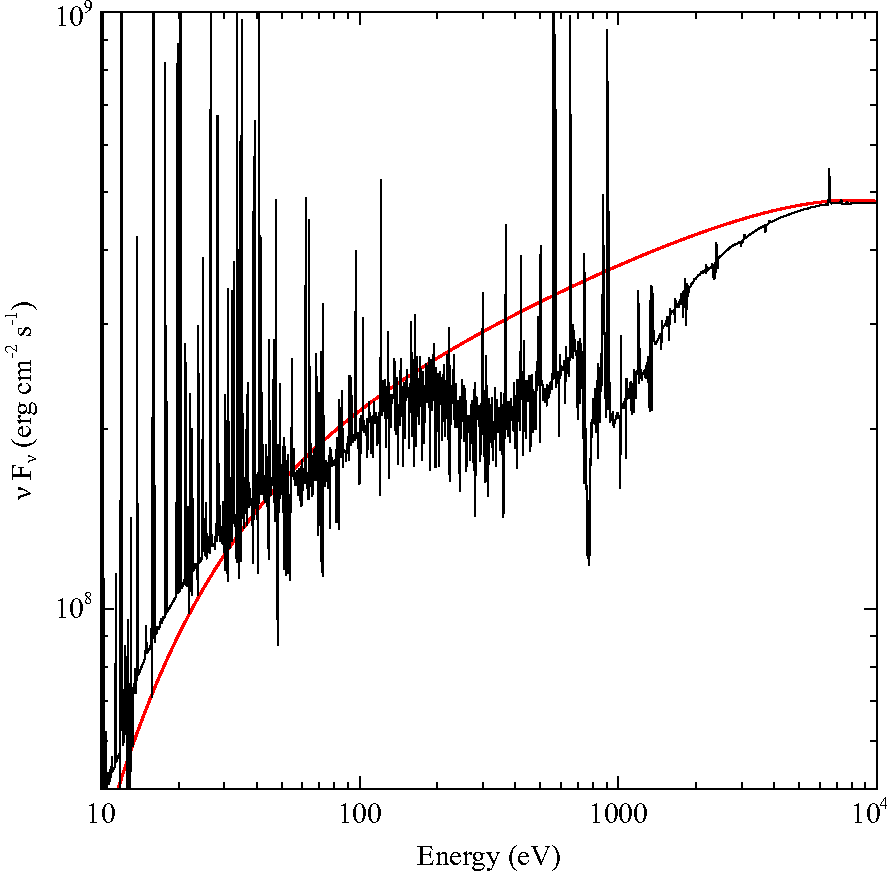
\includegraphics[scale=0.9]{WarmAbsorberReynoldsFabian}
\caption[Incident and net emission]{
\label{fig:WarmAbsorberReynoldsFabian}
The predicted X-ray spectrum of a warm absorber 
in an Active Galactic Nucleus. Prominent emission and absorption lines are present along with broad 
UTA absorption features. The parameters are from Reynolds \& Fabian (1995, MNRAS, 273, 1167).}
\end{centering}
\end{figure}

\subsection{Emission line -- continuum contrast}

In a real spectrometer the line-to-continuum contrast
depends on the spectrometer resolution if a line is unresolved.
The higher the resolution, the higher the line will appear in the spectrum.
In \Cloudy, lines are  unresolved on the coarse continuum mesh that is reported
in most versions of the \cdCommand{save continuum} command.
\Cloudy\ adds the emission-line intensities into the continuum, including the resolving power,
using Equation \ref{eqn:LineContinuumContrastFactor}.

When you plot the SED that is reported by a \cdCommand{save continuum}
command, emission lines will appear to have a triangular shape (assuming they
are not blended with lines in adjacent cells). We will treat this triangular
shape as the unresolved line profile. The total flux in that line will then be
given by the integral over this line profile, i.e. the area of the triangle.
This implies that when you perform an integral over the spectrum (e.g. to do
synthetic photometry) the line fluxes will automatically be included correctly
in the integral.

Real spectrometers may have significantly higher or lower resolution than 
\Cloudy 's coarse continuum.
The \cdCommand{set save line width / resolution} command,
described on page \pageref{sec:CommandSetSaveLWidth}, 
changes the lines relative to the continuum to make the spectrum
look like that observed with a spectrometer with a resolution that is different
from the coarse continuum.
Changing the velocity width with the
\cdCommand{set save line width} command  
has the same effect as changing the 
velocity resolution of a spectrometer measuring an unresolved line.
Smaller velocity widths will make the line rise higher above the continuum,
as shown in Equation \ref{eqn:LineContinuumContrastFactor}.
Alternatively you can also use the \cdCommand{set save resolution}
command to specify the spectral resolution of a spectrograph. Higher
values for the resolution will make the line rise higher above the continuum.

Note that this command will {\em only} adjust the height of the line, not the
width. The latter will always be the width of one cell in the coarse continuum mesh
({\em even if the line is broader than that cell}). This implies that
the line flux in the continuum array is artificially changed by the
\cdCommand{set save line width / resolution} command.
Changing the spectral resolution can be useful to emphasize weak lines in a plot,
but should never be used when energy conservation is important, e.g. when
you want to postprocess the file to fold the saved continuum with a photometric passband.

\subsection{Pumped contributions to the lines}

Continuum pumping and fluorescence are included as excitation processes
for all lines.
These contributions are usually not printed as a separate
quantity but will be if the \cdCommand{print line pump} command is entered.  Whether or not the pumped contribution actually
adds to the observed line emission depends on the geometry.
Continuum
pumping increases the line emission if no related continuum absorption is
seen by the observer.
This will be the case if the continuum source is
either not observed or not covered by absorbing gas on the observer's line
of sight.
If absorbing gas covers an observed continuum source then the
situation is like the P Cygni problem, emission produced by absorption
and pumping will not increase the total intensity of the line at~all.

The line intensity includes fluorescent excitation unless the
\cdCommand{no induced processes} command is entered.
That command is unphysical since it turns
off all induced processes.
You can judge how great the contribution of
the pumped part of the line is by printing it with the
\cdCommand{print line pump} command.

In general the treatment of scattering is very geometry dependent.
The
output produced by the \cdCommand{save continuum} commands \emph{does not} include the pumped
part of the line contribution.
This is correct if the continuum source
is included in the beam, but is not if only the gas is observed.

\subsection{Isotropic Continua}
\label{sec:save_cont_no_isotropic_option}

\par
By default the radiation field used in the calculation is reported. 
The CMB will often dominate certain portions of the spectrum,
overwhelming local emission, when it is included.
Most spectrometers in the radio and infrared will automatically remove  
isotropic emission while conducting an observation.
The \cdCommand{no isotropic} option provides a way to do a similar subtraction.
Each of the commands that set an SED shape,
described in Section~\ref{sec:IncidentContinuumShape}, will say
whether that component is isotropic or beamed.
This option will remove all sources of isotropic emission.

The commands
\cdCommand{save continuum} and
\cdCommand{save transmitted continuum}
have a \cdCommand{no isotropic} option
to not include attenuated isotropic continua in the total.
It is also possible to remove isotropic continua with the
 \cdCommand{no isotropic continua report} command described
in section \ref{sec:no_isotropic_continua}.

\subsection{The units option - changing the continuum units}
\label{output_units}
\label{units_option}

By default, the energy units for the first column, which gives the
wavelength or energy for each point in the continuum, are Rydbergs.  The
units can be changed to any of several energy or wavelength units with the
\cdCommand{units} keyword that appears on a \cdCommand{save continuum} command.  The following
keywords are recognized: \cdCommand{\_micron}, \cdCommand{\_eV\_}, \cdCommand{\_keV},
\cdCommand{\_MeV}, \cdCommand{wavenumber}, \cdCommand{centimeter} (also
\cdCommand{\_cm\_}), \cdCommand{\_mm\_}, \cdCommand{\_nm\_}, \cdCommand{Angstrom},
\cdCommand{\_Hz\_},\cdCommand{\_kHz}, \cdCommand{\_MHz}, \cdCommand{\_GHz},
\cdCommand{Kelvin} (also \cdCommand{\_K\_}), \cdCommand{erg\_}, and
\cdCommand{\_Rydberg}.
Both the keyword \cdCommand{units} and one of
these units must appear for the units of the energy scale to be changed.

\subsection{Save continuum uses vacuum wavelengths}
Vacuum wavelengths are always used in \cdCommand{save continuum} output.
This is to avoid a discontinuity at 2000\AA, the point where line wavelengths switch from
vacuum to air.
The \cdCommand{print line vacuum} command, 
described in section \ref{sec:CommandPrintVacuum},
controls whether line wavelengths
are given in air or vacuum, has no effect on \cdCommand{save continuum} output.

\subsection{Units of the save output in intensity and luminosity cases}
The units of the predicted continuum depend on whether the intensity
or luminosity case is used.
In the intensity
case continua are given as the intensity per octave
$ 4\pi \,\nu J_\nu [\ergpscmps ]$.
In the luminosity case they are
$\nu L_\nu$
[$\ergps $].
The emission from the cloud includes a covering factor if one was specified.

Through C13, the \cdCommand{save continuum} output 
in the luminosity case was per unit
cloud area at the inner radius rather than the true luminosity,
and so had units $\ergpscmps$.
This was to avoid processor limits on older computers.
Beginning in C16 output is in true luminosity units, $\nu L_\nu$, in the luminosity case.
The old behavior will the used if the
\cdCommand{set save luminosity old} option, described in
section \ref{sec:SetSaveLuminosity}, is used.
This is to provide backwards compatibility.

\subsection{Save continuum}

The \cdCommand{save continuum} command,
with no other keywords,
produces a file
with the following information.
The different contributors to the continuum
are defined in the Chapter \cdSectionTitle{Definitions}.

\begin{description}
\item[Column 1.]  The first column gives the photon energy in the units set
with the \cdCommand{units} option.  The default
units are Rydbergs.

\item[Column 2.]  This is the incident continuum at the illuminated face of
the cloud.

\item[Column 3.]  This is the transmitted incident continuum and does not include
diffuse emission from the cloud.
The cloud is assumed to fully cover the continuum source along our sight line, so a covering
factor has no effect.
If the option \cdCommand{no isotropic} has been issued, the transmitted continuum
does not include contributions from isotropic incident radiation sources.

\item[Column 4.]  This is the outward portion of the emitted continuum and line
emission.  This includes a covering factor if one was specified.
This does not include
the attenuated or reflected portions of the incident continuum.

\item[Column 5.]  This gives the net transmitted continuum,
the sum of the
attenuated incident (column 3) and diffuse (column 4) continua and lines.
This would be the observed continuum if the continuum source were viewed
through the gas.  Emission from the cloud includes a covering factor if one was specified.
If the option \cdCommand{no isotropic} has been issued, the net transmitted continuum
does not include contributions from isotropic incident radiation sources.

\item[Column 6.]  This is the reflected continuum
and is only predicted for an open geometry.

\item[Column 7.]  This is the total, the sum of the transmitted and reflected continua
and lines.  The attenuated incident continuum is included.
If the option \cdCommand{no isotropic} has been issued, the total continuum
does not include contributions from isotropic incident radiation sources.

\item[Column 8.] The sum of all reflected line emission.

\item[Column 9.] The sum of all outward line emission.

\item[Column 10 and 11.]  Line and continuum labels indicate the lines and
continuum edges that might contribute at that energy.  The line label gives the
label for the strongest line in the total spectrum (reflected plus outward) 
the line-center of which lies in that bin. 
(This is new in C10.  All previous versions simply reported the first line 
encountered, as is still the case with the continuum label.)   
The continuum labels are established when the code
is set up and they do not mean that the continuum feature is actually
present in the spectrum.  

\item[Column 12.]  This gives the number of emission lines within that continuum
bin, divided by the ratio of the energy width of the cell to the cell's
central energy, $dE/E$.  So this is the number of lines per unit relative
energy.
\end{description}

\noindent
This command will save the continuum at the outer edge of the cloud unless the
keyword \cdCommand{every} appears on the command line, in which case it will
save the continuum for every zone.

\subsection{What is observed}

Figure \ref{fig:EmissionSaveComponents} illustrates several
possible geometries.
Two lines of sight to the central object are shown,
and two clouds are shown.
Each cloud produces both a reflected and transmitted emission component.

\begin{figure}
\centering
\begin{centering}
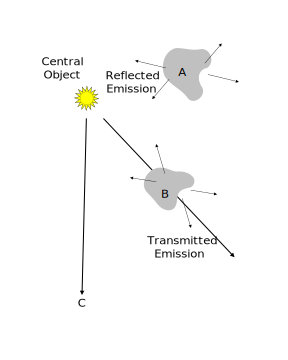
\includegraphics[scale=0.9]{EmissionSaveComponents}
\caption[Radiation field components in save continuum]{
\label{fig:EmissionSaveComponents}
This figure illustrates several components of the radiation field that enter in
the calculations.}
\end{centering}
\end{figure}

Three possible geometries, indicated by the letter on the figure, occur
depending on how we view the central source and clouds: a) we do not directly
observe the central object although we may see it by reflection from the
illuminated face of a cloud, b) we observe the transmitted continuum and
the outward emission from the emitting cloud, and c) we observe the
unattenuated continuum directly without absorption.
Column 2 gives the
unattenuated continuum, and column 3 gives the attenuated continuum.

There are also three possible situations for the line emission.
First,
we might only observe clouds that lie on the near side of the continuum
source.
In this case we see the ``outward'' line emission.
Second, we
might only observe clouds that lie on the far side of the continuum source.
In this case we only see the ``reflected'' or inward component.
Lastly,
we might observe a symmetric geometry with reflected emission from the far
side and outward emission from the near side.

In most cases an observer at large distance from the structure would
observe \emph{both} the central object and the cloud and would measure the quantity
listed in column 5 (if only transmitted emission is detected) or column
7 (if both reflected and transmitted continua are seen).  If the central
object is not seen then the quantity in column 4 would be observed.

\subsection{Save continuum bins}

This saves the continuum energy bins.
The first column is the center
of the bin in whatever unit was set after the \cdCommand{units} keyword
(see Section~\ref{units_option} for details).
The second column is also the center of the bin, but this time always in Ryd.
The third column is the cell width $\delta\nu$, also in Ryd.
The bin extends from $\nu-\delta\nu/2$ to $\nu+\delta\nu/2$.

\subsection{Save cumulative continuum}
\label{sec:CommandSaveCumulativeContinuum}

This gives the continuum integrated over a time-dependent simulation.
The usual \cdCommand{save continuum} command gives the
continuum for the current time step in these calculations.
The units of the usual \cdCommand{save continuum} command
are flux per octave, $\nu f_{\nu}\; [\ergpscmps ]$.
This command gives the time-integrated energy,
$\nu E_{\nu}\; [\ergpscm ]$.

\par
Note that using this command with the option \cdCommand{no isotropic}
will cause \Cloudy\ to exit immediately with an error message.

\subsection{Save diffuse continuum}

This reports the local diffuse line and continuous emission
coefficient $4 \pi \nu j_{\nu}$ [\ergpccmps ].
Optical depth effects are not included.

By default this reports the diffuse emission from the last zone.
The first column of the output gives
the photon energy including the \cdCommand{units} option.
The second column gives the diffuse continuous emission.
The third column gives the line emission in the same units,
including the effects of the
\cdCommand{set save line width / resolution} command described on page
\pageref{sec:CommandSetSaveLWidth} when appropriate.
The last column gives the total.

If the keyword \cdCommand{zone} appears then the diffuse emission
\emph{from every zone} will be reported.
The first row gives the wavelength or energy scale.
The remaining rows give the total (line and continuum)
emission coefficients $4 \pi \nu j_{\nu}$
at each energy.

\subsection{Save continuum emissivity 12 [units micron]}

This command will save the continuum volume emissivity $4\pi \nu j_\nu$ (in
\ergpccmps), as well as the local absorption and scattering opacity (in
cm$^{-1}$) as a function of radius and depth (in cm). This output can be used by an
external program to do more specialized radiative transfer, e.g.\ to determine
the continuum flux through an aperture. To make this process second-order
accurate, the radius and depth in the middle of each zone is reported. One number should
be supplied on the command line, which is the wavelength / frequency at which
the emissivity and opacity will be evaluated. You can use the keyword
\cdCommand{units} as described in Sect.~\ref{output_units}. By default the
frequency is assumed to be in Rydberg.

\subsection{Save emitted continuum}

The continuum emitted and reflected from the nebula is saved.
The
first column is the photon energy.
The second column is the reflected
spectrum.
The third column is the outward diffuse emission.
The fourth
column is the total emission (the sum of the inward and outward emission).
This would be the observed emission from the nebula if the central continuum
source was not in the beam but clouds uniformly cover the continuum source.
The last two columns are labels for lines and continua contributing at each
energy.
The attenuated incident continuum is not included in any of these
components.
The effects of a covering factor are included.
The continua have units
$\nu f_{\nu}$ [\ergpscmps ] or $\nu L_{\nu}$ [\ergps ] 
depending on whether the intensity or luminosity case is specified.

\subsection{Save fine continuum [range, merge]}

The code transfers the continuum on a coarse mesh, needed for speed in
evaluating photo-interaction rates, and on a fine mesh, needed for automatic
treatment of line overlap.
The coarse continuum is the one given in output
from the \cdCommand{save continuum} command and it includes all the components shown in Figure \ref{fig:EmissionSaveComponents}.
The fine continuum is designed to account for line transfer.
It shows a normalized attenuated incident continuum and 
does not include continuous
emission or absorption from the cloud.  
This multi-grid approach is needed to combine
precision and speed.  This command reports the line transmission coefficient,
$I_{transmitted}/I_{incident}$, for the fine continuum.

The resulting output will be huge if the entire fine continuum is saved.
The command accepts a \cdCommand{range} option to limit the size of the output file.
If the keyword \cdCommand{range} appears then
the lower and upper limits to the range
of the fine continuum must be entered.
The command also accepts
a \cdCommand{units} option,
described on \pageref{output_units}, to change the units used
in the specified energy range, and in resulting output.

The optional third numerical parameter gives the number
of fine continuum cells to average together, again with the intent of
reducing the size of the output file.  The default is to average over 10
cells.  If the number of cells to be combined is specified then it must
be the third number on the command line, following the limits
of the range.

The resolving power of the fine continuum is adjusted when the calculation begins so
that lines of the heavy elements can be resolved.
The resolving power is reported in the main printout with the string
\cdCommand{R(F~Con)}.

\subsection{Save grain continuum}

The thermal emission by grains is part of the emergent continuum.  This
command saves only the grain emission in the optically thin limit for
the last zone.  It is mainly intended as a debugging aid.

The first column gives the photon energy in the units specified with
the \cdCommand{units} option.  The second column gives the total emission from
carbonaceous grains (including amorphous carbon and PAH's).  The third column
gives all emission from all constituents that are not carbonaceous.  In
practice this will be mainly the silicates.  The last column gives the sum
of the two.

\subsection{Save incident continuum}
\label{sec:CommandSaveIncidentContinuum}

The incident continuum, that emitted by the central object and striking
the illuminated face of the cloud, will be saved.  The first two columns give
the photon energy and the continuum specific intensity 
$\nu 4\pi J_{\nu}$ [erg cm$^{-2}\ \mathrm{s}^{-1}$] 
or specific luminosity 
$\nu L_{\nu}$ [erg  $\mathrm{s}^{-1}$].
The photon occupation number 
\begin{equation}
{\eta _\nu } \equiv {J_\nu }\left( \nu  \right)\,{\left( {\frac{{2h{\nu
^3}}}{{{c^2}}}} \right)^{ - 1}}
\end{equation}
concludes the line.

\subsection{Save interactive continuum}

This gives the product of the internal radiation field times the gas opacity integrated over the full continuum.  
The results are produced for each zone and give
the attenuated incident continuum, the OTS line, the OTS continuum, the
outward continuum and the outward lines.  The first optional number is the
lowest energy in the output.  If missing or zero, the lowest energy
considered by the code will be used.  Numbers less than 100 are interpreted
as the energy in Rydbergs and those greater than 100 as the cell number.

\subsection{Save ionizing continuum [options]}

This creates a file that can be used to indicate ionization sources.
If the keyword \cdCommand{every} occurs then this is saved for every zone, otherwise
it is only saved for the last zone.

The first optional number on the command line is the lowest energy to
include in the output.  If it is missing or zero then the lowest energy
considered by the code will be used.  It is interpreted as the energy in
Rydbergs if the number is less than 100 and as the cell number if it is
greater than 100.  The second optional number is the threshold for the
faintest interaction to print.  The default is one percent of the quantity
given in the \cdMono{rate/tot} column.
Enter zero for this number if you want
all interactions to be printed.  The optional numbers may be omitted from
right to left.

The first column in the resulting output is the cell number
of the C scale, so the first cell is zero.
Next comes the photon energy
in Rydbergs unless changed with the \cdCommand{units} option.  The third column, with
the header \cdMono{flux}, is the flux of photons within this frequency bin
(\emph{not}
per unit frequency) with units s$^{-1}$~cm$^{-2}$.  The forth column gives the
photo-interaction rate, the product of the flux multiplied by the gas
absorption cross section
[cm$^{-2}$] and so with units s$^{-1}$.  The next five numbers are the fractions of
this photo-interaction rate due to the attenuated incident continuum, the
OTS line, the OTS continuum radiation fields, and the outward lines and
continua.  The 10$^{\mathrm{th}}$ column, with the heading \cdMono{rate/tot}, is the ratio
of this photo rate to the total integrated radiation-field interaction rate.
The next column, with the heading \cdMono{integral}, is the integrated cumulative
interaction, the integral of the previous column over energy.  This makes
it easy to identify the portions of the radiation field that have the
dominant interaction with the gas.  The last two labels on the line indicate
which lines and continua contribute at that energy.

\subsection{Save raw continuum}

This saves the \cdTerm{raw} continua.
This is exactly the continuum used
within the code.  The first number is the photon energy.  The next columns
are the contents of many of the continuum arrays at each energy.  Consult
the source to see which arrays are now saved.  Each gives the number of
photons stored in that cell with units photons s$^{-1}$ cm$^{-2}$
cell$^{-1}$.  The last
number is the number of lines within that cell.

\subsection{Save reflected continuum}

The reflected continuum is output if \cdCommand{sphere} is not set.  The first column
is the photon energy, the second the reflected continuum $4\pi \,\nu J_\nu
$ [erg  cm$^{-2}$~s$^{-1}$] at that energy.  The third gives the reflected lines
and the fourth is the sum of these two.  Someone who could only see the
illuminated face of the cloud would observe this.  The next column is the
effective albedo of the cloud, the ratio of the reflected to incident
continuum (the \cdCommand{save total opacity} command will give the
true albedo).  The last column gives the label
for continuum processes with thresholds at each energy.

\subsection{Save transmitted continuum [no isotropic]}
\label{sec:CommandSaveTransmittedContinuum}

This saves the transmitted spectrum (i.e., the attenuated incident SED and the outward component
of the diffuse continuum and line emission) predicted at the end of the calculation.
It is affected by the \cdCommand{no isotropic} option.

This save file can be used as part of the incident continuum in a later
calculation by reading it with the \cdCommand{table read} command described in
Section \ref{sec:CommandTableRead}.

The code will implicitly behave as if the keyword \cdCommand{last} had been
included. This is needed since the code would become confused if it tried to
read a file containing information from multiple iterations. So the output
would be useless without this keyword. In a grid run it will also implicitly
save the continuum into a separate file for each grid point. This is needed
for the same reason: the code cannot read a concatenated output file.

Two cautions apply when reading this file as an input continuum. First, save
output should not be written into the same file as the input file during the
second calculation. The file containing the first continuum will be
overwritten if this occurs. Second, the first couple of lines contain header
information that is needed by the code. They should not be deleted.

This command is unusual in that it always saves the SED in intensity units,
even when the simulation is done in luminosity mode. If the radius is set, the
continuum will be an intensity normalized at the outer radius. If the radius
is not set, the intensities will have the usual normalization also used in
other \cdCommand{save continuum} commands.

The line-to-continuum contrast factor \cdVariable{Resolution}
set by the \cdCommand{set save line width / resolution} command
(see page \pageref{sec:CommandSetSaveLWidth})
is not used in this command.  This is to insure that lines have
the correct intensity in the save file, as needed for energy conservation.
The \cdCommand{units} keyword is also ignored. The output will always use
the standard unit (Rydberg) as the frequency unit.

\subsection{Save two photon continuum}

This saves the total two-photon continuum and is mainly a debugging
aid.  The photon energy is followed by the number of photons emitted per
Rydberg per second, then by $\nu F_\nu$.  The details of two photon emission,
including induced processes, are discussed by \citet{Bottorff2006}.

\section{Save convergence [reason, error]}

These commands produce information about various aspects of the converged
solution.

\subsection{Save convergence base}

The gives computed values of many quantities that are converged during
a calculation.  The values are given as they are at the exit to the base
convergence routine.  Depending on the convergence properties of the
solution, there will be between only a few up to many
dozens of evaluations in each zone.

\subsection{Save convergence error}

This will produce information concerning the quality of the converged
pressure, electron density, and heating-cooling solution.  The correct value,
converged value, and percentage error, (correct-converged) $\times$ (100/correct), will be produced for each zone.

\subsection{Save convergence reason}

This will save the reason the model was declared ``not converged'' at
the end of each iteration when the
\cdCommand{iterate to convergence} command is used.

\section{Save cooling}

This saves the cooling agents for each zone.  The first number is the
depth [cm] followed by the temperature [K].  The next two numbers are the
total heating and cooling rates [erg cm$^{-3}$~s$^{-1}$].  The remaining labels
indicate contributors to the cooling array and the fraction of the total
cooling carried by that agent. The faintest coolant saved is normally
0.05 of the total and can be reset with the \cdCommand{set WeakHeatCool} command.

This is mainly used for debugging and its output is not well documented.
The line labels may, or may not, correspond to labels used in the main
emission-line output.  The code adds individual coolants to the total cooling
by calling routine \cdRoutine{CoolAdd}.
The arguments to that call include the string
and a number that follows it.   To discover the process for a particular
label you will need to search over the entire code to find where that string
occurs in a call to \cdRoutine{CoolAdd}.
The string will be within a pair of double
quotes.
As an example, two coolants that might appear are
\cdTerm{dust 0}, and \cdTerm{H2cX 0}.  A search on the string \cdMono{"H2cX"} (include the beginning and ending double
quotes) will find the string occurring in two places, where the cooling
is added with the call to \cdRoutine{CoolAdd} and another place where the cooling itself
is evaluated.  Comments around the call to \cdRoutine{CoolAdd}
indicate that \cdTerm{H2xC} is
cooling due to collisional excitation within the ground electronic state
of \htwo.   A search on the string \cdMono{"dust"} finds its call to
\cdRoutine{CoolAdd} with
the comment that it is cooling due to grain recombination cooling.

Cooling due to the unified iso-electronic sequences is different since
the label that occurs in the call to \cdRoutine{CoolAdd} is generated by the routine
that evaluates the cooling and does not explicitly occur in the source.
The iso-electronic cooling labels begin with \cdMono{"IS"},
followed by a string
indicating the process, and followed by strings giving the iso-electronic
sequence and the element.  Search for the start of the string but not for
the element name.  An example might be the string
\cdMono{"IScionH H"}.  The \cdMono{"IS}
indicates that it is cooling due to an ion along the iso-electronic sequences
and the two ending H's indicate that the coolant is H-like hydrogen.  The
string \cdMono{"IScion"} occurs in the source and comments indicate that the process
is collisional ionization cooling.  The iso-electronic cooling strings do
not include a pair of double quotes in the source since the ending double
quote occurs after the element names.  You would search for the string
\cdMono{"IScion"}.

\subsection{Save cooling each}

If keyword \cdCommand{each} appear after \cdCommand{save cooling}
command, the cooling of each element and for certain
special cases will be saved for each zone. 
The unit of the cooling rate is [erg cm$^{-3}$~s$^{-1}$]. 
Notice that the output metal bremsstrahlung cooling is the real 
metal bremsstrahlung cooling minus the total bremsstrahlung heating. If the
bremsstrahlung heating is comparable with the real metal bremsstrahlung cooling,
the output may not be precise.
The cooling due to molecules is listed separately. The total cooling
listed in column 3 does not include the dynamics cooling (adve, column 45).

\section{Save charge transfer}

Charge transfer recombination and ionization rate coefficients
   [cm$^3\mathrm{s}^{-1}$]
for hydrogen onto heavier elements will be output.  The rates will be
evaluated at the temperature of the last computed zone.  Rates for
recombination (${\mathrm{A}}^{ + x}  + {\mathrm{H}}\to{\mathrm{A}}^{ + x + 1}  + {\mathrm{H}}^
+$) are first, followed by the rates for the opposite ionization process.
The first number is the atomic number of the species.

\section{Save Chianti}
\label{sec:CommandSaveChianti}

This saves collision strengths for Chianti transitions over a certain temperature range.
The output gives species, lower level, upper level, wavelength in Angstroms, 
and collision strengths for each temperature given in the header row.
This reports data for all active Chianti species in that particular run.

\section{Save dr}

The logic behind the choice of zone thickness will be described.

\section{Save dynamics options}

This produces some information concerning the dynamics solutions.

\subsection{Save dynamics advection}

This produces information about advection terms.

\section{Save element \emph{name}}

This will save the ionization structure of any element. The output will
have one line per zone giving the ion fraction\footnote{Before version 96 the ionization fractions only included atoms and
ions.  They now include molecules.  The sum of the atomic and ionic fractions
will not add up to unity if a significant fraction of the element is in
molecules.} of each successive stage
of ionization.  The keyword \cdCommand{element} must be followed by the element name.

The first number on the resulting output is the depth [cm] into the cloud.
The remaining lines give the relative ionization fraction of the $n+1$ possible
stages of ionization where $n$ is the atomic number of the element.  These
may be followed by some of the more abundance molecules.

If the keyword \cdCommand{density} appears on the command line then the
density [cm$^{-3}$]
will be given rather than the dimensionless fraction.

\section{Save enthalpy}

The file will list the depth into the cloud, followed by the total
enthalpy, and various contributors to it.

\section{Save execution times}

The code will output the zone number, the time required to compute that
zone, and the elapsed time since the start of the calculation.  This is
intended as a mechanism to identify zones that require large amounts of
work to converge.  
This command is being superseded by the \cdCommand{save performance} command.

\section{Save FeII}
\label{sec:CommandSaveFeII}

These commands are obsolete.
See the \cdCommand{save species} family of commands,
Section~\ref{sec:SaveSpecies}.

\section{Save FITS}

This command produces photon energies and the total transmitted continuum into
a two-column file in FITS (Flexible Image Transport System) format.  FITS
is a standard format used in astronomy, and endorsed by both NASA and the
International Astronomical Union.  The most current definition of the FITS
format is by \citet{Hanisch2001}.  This was added by Ryan Porter and its
first application is given in \citet{Porter2006}.  The saved spectrum will
by default include the isotropic continua.  They can be excluded using the
\cdCommand{no isotropic continua report} command.  The saved spectrum will
always conserve energy, i.e. the \cdCommand{set save resolving power} command
has no effect.

Since only one spectrum can be stored in a FITS file, the command will
implicitly behave as if the keyword \cdCommand{last} was included on the
command line.

The following creates a FITS file with a blackbody continuum
\begin{verbatim}
blackbody 1e5 K
ionization parameter -2
save FITS "filename"
\end{verbatim}

This command is often used with the \cdCommand{grid} command which creates
grids of calculations. In this case, the command produces separate FITS files
for each grid point. They will have names
\cdFilename{grid000000000\_filename}, \cdFilename{grid000000001\_filename},
etc., where \cdFilename{filename} is the file name you supplied between double
quotes. The meaning of the grid index embedded in the filename can be found with
the \cdCommand{save grid} command described in Section~\ref{sec:save:grid}.

\section{Save gammas}

This gives the photoionization rates for all subshells of all ions for
the last zone.  The numbers are the element, ion, and subshell numbers,
followed by the photoionization and heating rates from that subshell.  The
remaining numbers are the fractional electron Auger yields.

\subsection{Save gammas element oxygen 1}

If the \cdCommand{element} keyword appears then the detailed contributors to the
photoionization rate for the valence shell of a particular element will
be produced by calling \cdRoutine{GammaPrt}.
The ionization stage must also appear,
with 1 the atom, 2 the first ion, etc.

\section{Save Gaunt factors}

This produces a series of tables showing the thermally averaged free-free
Gaunt factors as a function of the log of the photon energy (vertical, in Ryd)
and the log of the electron temperature (horizontal, in K). Such a table is
produced for each charge state treated by \Cloudy. Below each table, the Gaunt
factors are repeated as triplets, but this time as a function of the customary
dimensionless units $\log \gamma^2$ and $\log u$ rather than temperature and
photon energy.

\section{Save grains [options]}

These commands give grain properties.  Several grain species are usually
included in a calculation.   Often there are several size bins per grain
type.  These commands will print a line giving a list of the grain labels,
followed by a line giving the grain radius in $\mu m$.
The following lines then give the individual grain properties
(temperature, potential, etc) for each size and type.

Details of the grain physics are given in \citet{Baldwin1991},
\citet{Weingartner2001a},
\citet{VanHoof2004}, and \citet{Weingartner2006}.

\subsection{Save grain abundance}

The grain abundance [g cm$^{-3}$] for each grain bin and the total grain
abundance is given as a function of depth.

\subsection{Save grain charge}

The first number is the electron density [cm$^{-3}$] contributed by grains.
A positive number indicates that grains where a net source of electrons
so they have a net positive charge.  The remaining columns print the charge
of each grain size and type, in number of elementary charges per grain,
for each zone.

\subsection{Save grain continuum}

This is listed in the \cdSectionTitle{save continuum} section.

\subsection{Save grain D/G ratio}

The dimensionless dust to gas ratio for each grain bin and the total
grain abundance is given as a function of depth.

\subsection{Save grain drift velocity}

The drift velocity [km s$^{-1}$] of each grain species is printed for each zone.

\subsection{Save grain extinction}

The grain extinction at the $V$ filter will be saved as a function of
depth.  This extinction only includes grains, although they should provide
nearly all the extinction when they are present.  The first column gives
the depth into the cloud [cm], the second is the extinction [mag] at the
$V$ filter for an extended source, like a PDR, and the third number is the
extinction for a point source like a star.  This distinction is discussed
in Sections 7.2 and 7.6 of AGN3.  The extended source extinction discounts
forward scattering by writing the scattering opacity as $\sigma ( 1-g )$,
where $\sigma$ is the total scattering opacity and $g$ is the grain asymmetry
factor.
The quantity in the last column does not include the $({1-g})$
term.

\subsection{Save grain H2rate}

The grain \htwo\ formation rate is given for each size and type of grain
and for each zone.

\subsection{Save grain heating}

The grain heating [erg cm$^{-3} \mathrm{s}^{-1}$] is output for each zone.

\subsection{Save grain opacity}

This gives the grain opacity as a function of the photon energy in the last
zone of the model.  The first column is the photon energy in the units set
with the \cdCommand{units} option, the second the total (absorption plus
scattering) cross section, followed by the absorption and scattering cross
sections.  These are the summed cross section per proton for all grain
species in the calculation. Column 5 is the pure scattering cross section
summed over all grains and column 6 is the grain albedo.   Columns 2, 4,
and 6 use the scattering cross section multiplied by $(1-g)$, while column
5 does not. The opacities have units [cm$^{2}$ H$^{-1}$] using the actual
grain abundance from the last zone.

\subsection{Save grain potential}

 The grain floating potential [eV] is output for each grain size bin and
each zone. The grain potential is defined~as
\begin{equation}
\varphi _g  = \frac{{\left( {\left\langle Z \right\rangle  + 1} \right)e^2
}}{a}
\end{equation}
where $\langle Z\rangle$ is the average grain charge of the grain size bin.  In reality
there is a distribution of grain charges in each bin, so this quantity does
not relate to any individual grain. It is approximately the amount of energy
needed to move an electron from the grain surface (after it has been lifted
out of the grain potential well) to infinity, averaged over all charge
states.
\citet{Weingartner2001a}, \citet{VanHoof2004} and \citet{Weingartner2006} provide further details.

The grain potential given here and the (average) grain charge
(see \cdCommand{save grain charge}) differ only by constants.  It
is probably best to use the latter since that quantity will be far easier
to define. Refer to \citet{Weingartner2001a} and
\citet{VanHoof2004}
for more details.

\subsection{Save grain qs}

The photon energy in Rydberg is followed by the absorption and scattering
efficiency for each grain species. The absorption efficiency $Q_{\rm abs}$ is
defined as the ratio of the absorption cross section $\sigma_{\rm abs}$ and
the geometric projected grain surface area $\sigma_{\rm g} = \pi a^2$. This
yields: $Q_{\rm abs} = \sigma_{\rm abs}/\sigma_{\rm g}$. A similar definition
holds for the scattering efficiency, keeping in mind that the scattering cross
section has been multiplied by $(1-g)$, i.e., we print: $Q_{\rm scat} (1-g) =
\sigma_{\rm scat} (1-g) / \sigma_{\rm g}$. See also Chapter 7 of AGN3.

\subsection{Save grain temperature}

The temperature of each grain species is printed for each zone.

\section{Save grid}
\label{sec:save:grid}

This is used with the \cdCommand{grid} command to
create a file giving the parameters for each simulation in a large grid
of calculations.  This can be combined with other \cdCommand{save} commands to create
files giving the derived quantities for a large set of calculations.

The first row gives tab-separated column titles.  The column title for the parameters
that are varied will give the first few characters of the command line for
that parameter.  Each of the following lines summarizes a particular grid point.  The
first column gives the index number in the grid. This is useful if you
have separate output for each grid point (e.g. from the \cdCommand{save FITS}
command). The index number will be part of the file name in that case. It is
also useful for finding back the output from a particular grid point in a
save file (see Section~\ref{sec:GridOutputOptions} for more details).
The next two columns indicate whether the calculation had a failure or had any
warnings.  A successful calculation will have ``F'' (for false) indicating
no failure or warning occurred.  If either of these is ``T'' (for true) then
that simulation had major problems. The following column is a string giving
a bit more detail about the exit code. It says ``ok'' if everything went fine
and ``warnings'' if warnings were present in the run, but nothing more serious.
If the simulation failed completely, you could see strings like ``cloudy abort''
or ``early termination''. You should look at the detailed output
to find out what went wrong. The next two columns give the number of the
MPI rank that executed the simulation (will be zero in non-MPI runs) and the sequence
number of the simulation on that rank (they are executed in random order). These
numbers are used for debugging the code. The next columns give numerical parameters for
each simulation in the grid.  The last column gives all the grid parameters
as a single string.  Many plotting programs will allow you to add this string
next to each of the plotted data points.

This command does not produce any output if the \cdCommand{grid} command
is not used. In grid runs it is highly recommended to always include this command.
It allows you to see in one glance if the run was successful and where the problems
are in case it was not. It is also useful to include this output in case you want
to file a bug report.

\section{Save heating}

The code will save the heating agents for each zone.  The first two columns
give the depth [cm] and temperature [K].  The next two columns give the
total heating and cooling rates [erg cm$^{-3} \mathrm{s}^{-1}$].  This is followed by a set
of labels for various heat sources and the fraction of the total heating
carried by that agent.  The faintest agent saved is normally 0.05 of the
total and can be reset with the \cdCommand{set WeakHeatCool} command.

The heating labels will probably not correspond to any entries in the
emission-line list.  If the identification of a heat source is in question
the best recourse is to search for the heating label over the entire code.

\section{Save [option] history}

\subsection{Save pressure history}

This follows the pressure and density convergence history.

\subsection{Save temperature history}

This follows the temperature and heating---cooling convergence history.

\section{Save H2}

Some details of the large \htwo\ molecule are output as a save file.  One
of the following options must appear.  The large \htwo\ model is not enabled
by default but is turned on with the \cdCommand{database H2} command.

Many studies of \htwo\ properties will use plots showing populations as a
function of excitation energy.  The slope gives a population temperature,
which may be related to the kinetic temperature under some circumstances.
Theoretical plots can be made using the
\cdCommand{save H2 column density}
or \cdCommand{save H2 populations} commands described below.
The level energy in K, given in
the save output, is the x-axis and the column density or population in
each level is the y-axis.

The \cdCommand{save grain H2rate} command gives
the \htwo\ formation rate for each of the grain species included in the calculation.

\subsection{Save H2 column density}

This saves the column density of ro-vibrational states within the ground
electronic state.  This command recognizes the same options as the \cdCommand{save H2 populations} command.

The file begins with the total \htwo\ column densities
in the ortho and para forms, followed by the total \htwo\ column density.  The remainder of the file
gives the $v$ and $J$ quantum indices, followed by the excitation energy of
the level in K, the total column density in that level, and finally the
column density divided by the statistical weight of the level.

\subsection{Save H2 cooling}

This produces a file containing heating and cooling rates
[$\pcc\ \ps$] as a function of depth.

\subsection{Save H2 cooling per molecule}

This produces a file containing the LTE cooling (for transitions within the X band only),
and the net H2 cooling (cooling minus heating) as a function of temperature.
Each measure of cooling is reported per H2 molecule in units of \ergps.

\subsection{Save H2 creation}

This command has been superseded by the \cdCommand{save chemistry rates} command.

\subsection{Save H2 destruction}

This command has been superseded by the \cdCommand{save chemistry rates} command.

\subsection{Save H2 heating}

This produces a file containing the depth, total heating rate [erg
cm$^{-3}\mathrm{s}^{-1}$], and \htwo\ heating predicted by an expression in \citet{Tielens1985a}, together with the heating predicted by the large model of the \htwo\ molecule.

\subsection{Save H2 levels}

This creates an energy-ordered list of the levels within X.  The first
column gives the energy in wavenumbers relative to the lowest level, the
second gives the statistical weight, and the next two columns give the
vibration and rotation quantum numbers.  The sum of the transition
probabilities is given, followed by the sum of collisional de-excitation rate
coefficients (cm$^{3}$ s$^{-1}$) of the level for each of the colliders 
included in the calculation.

\subsection{Save H2 lines}

The intensities of all significant \htwo\ emission lines that are produced
within the ground electronic configuration are given.  The file also gives the
information needed to convert an emission-line spectrum into a level
population vs excitation energy diagram.

Each line of output begins with a spectroscopic designation of the line,
followed by the upper and lower electronic, vibration, and rotation quantum
numbers.
This is followed by the wavelength of the line in microns.
The
line wavelength is then printed as it appears in the output.
The log of
the intensity or luminosity in the line (depending on whether the intensity
or luminosity case is specified), and the intensity of the line relative
to the normalization line, follow.
The excitation energy of the upper
level of the transition in Kelvin and the product
$g_u h\nu A_{ul} $  for each line are also given.
This product is needed to convert
intensities into excited-state column densities.

Only lines brighter than 10$^{-4}$ of the reference line are given by default.
The intensity of the faintest line, relative to the normalization line,
is set with the first optional number that can appear on the command line.
If the number is negative then it is interpreted as the log of the limit.

By default only lines within the ground electronic system are saved
but this can be changed if the keyword \cdCommand{electronic}
appears on the command line.
If the keyword \cdCommand{all} also appears then lines
within all electronic systems are saved.
If the keyword \cdCommand{ground} appears then only lines the
ground system are saved.  This is the default.  If a number appears then
it is the number of electronic systems to be saved, 1 for only the ground
electronic state.  If the number of systems is specified then it must be
the second number on the line---the first being
the intensity of the faintest line to print.

The following give examples.  The first sets the faintest \htwo\ line to
save.  Only lines within the ground electronic system will be produced.
\begin{verbatim}
save H2 lines, faintest -4 "filename"
\end{verbatim}
This sets the faintest line, and also requests all lines produced by all
electronic configurations.
\begin{verbatim}
save H2 lines, faintest -4 all "filename"
\end{verbatim}
This example requests only lines for the lowest three electronic
configurations.
\begin{verbatim}
save H2 lines, faintest -4 electronic 3 "filename"
\end{verbatim}

\subsection{Save H2 populations}

The level populations for the ground electronic state are given for the
last computed zone.  The populations are relative to the total \htwo\ abundance.

There are several optional parameters.
The quantum numbers of the highest
vibrational and rotational levels to save can be specified as consecutive
numbers on the command line.
These occur in the order $v$ then $J$.
If no
numbers occur, or if a limit that is less then or equal to zero is entered,
then populations of all levels will be saved.

If the keyword \cdCommand{zone} appears then the level populations 
will be saved for every zone.   These are all given along one long line,
a format that is different from the other output options.  Otherwise the
populations are only saved at the end of the iteration using the output
options described next.

If output is only saved for the last zone then it can be in either
a triplet format, with the vibration and rotation quantum numbers followed
by the population, or as a matrix, with all populations of a given vibration
quantum number lying along a single row.  The triplet form is done by
default, and the second will occur if the keyword
\cdCommand{matrix} occurs on the command line.

The \cdCommand{save H2 column densities} command provides similar output
options but for integrated column densities.

\subsection{Save H2 PDR}

The output contains six columns giving the depth (in cm), the
o-\htwo\ density, the p-\htwo\ density (both in cm$^{-3}$), and the Solomon
dissociation rate following \citet{Tielens1985a}, \citet{Bertoldi1996}, and
the \Cloudy\ big \htwo\ model, respectively (in s$^{-1}$).

\subsection{Save H2 rates}

The output contains useful information regarding \htwo\ formation and
destruction rates.

\subsection{Save H2 Solomon}

The output will give the total rate for photo-excitation from the ground
to electronic excited states and then identify those levels which are the
dominant contributor to the total rate.

\subsection{Save H2 special}

This provides infrastructure to save debugging information.  It can
be easily changed to suite particular needs.

\subsection{Save H2 temperatures}

The depth [cm], 21 cm spin temperature [K], gas kinetic temperature [K],
and several temperatures derived from relative populations of $J$ levels within
the H$_2\, v=0$ ground  electronic state [K], are saved for each zone.

\subsection{Save H2 thermal}

A variety of heating---cooling processes involving \htwo\ are given
for each zone.

\section{Save helium [options..]}

\subsection {Save helium line wavelengths}

This gives wavelengths of lines from $n=2$ levels of He-like ions.

\section{Save hydrogen}

\subsection{Save hydrogen 21 cm}

This gives some information related to the spin temperature of the 21
cm line.
The keyword is either \cdCommand{21 cm} or \cdCommand{21cm}.
The level populations
within 1s are determined including radiative excitation by \la, pumping by
the external and diffuse continua, collisions, and radiative decay.  Several
of the resulting populations and temperatures are included in the output.

\subsection{Save hydrogen conditions}

This gives the physical conditions and populations of various forms of
hydrogen are given as a function of depth.  The depth [cm], temperature
[K], hydrogen density [cm$^{-3}$], and electron density [cm$^{-3}$] are followed by
the densities of \hO, \hplus, \htwo, H$_{2^{+}}$, H$_{3^{+}}$, and H$^-$ relative to the total hydrogen
density.

\subsection{Save hydrogen ionization}

This gives rates for processes affecting the hydrogen ionization as a
function of depth.  The columns give the ground state photoionization rate
[s$^{-1}$], the total and Case~B recombination coefficients [cm$^3$~s$^{-1}$], the
predicted ratio of $n$(\hplus) to $n$(\hO), and the theoretical ratio for the simple
case.  Finally, contributors to the ground state photoionization rate are
produced with a call to \cdRoutine{GammaPrt}.

\subsection{Save hydrogen lines}

The upper and lower quantum indices, the line energy, and the optical
depth in the line, will be saved.

\subsection{Save hydrogen Lya}

This produces some information related to the excitation, destruction,
and escape of the \la\ line of hydrogen.  The optical depth from the
illuminated face to the outer edge of the current zone is followed by the
excitation temperature, electron kinetic temperature, and the ratio of these.

\subsection{Save hydrogen populations}

This gives the depth [cm], the densities of \hO\ and \hplus\ [cm$^{-3}$],
followed by the level population densities [cm$^{-3}$]
for the levels in the order $n = 1, 2s, 2p, 3, 4, 5,\dots$ for each zone.

\section{Save ionization means}
\label{sec:CommandSaveIonizationMeans} 

The mean\footnote{Before version 96 the ionization fractions only included atoms and
ions.  They now also include molecules.  The sum of the atomic and ionic
fractions will not add up to unity if a significant fraction of the element
is in molecular form.} ionization of all elements included in the calculation will
be output.  The format is exactly the same as the mean ionization printout
produced at the end of the standard output.

The \cdCommand{save averages} command described on
page \pageref{sec:CommandSaveAverage} can save
the average ionization fraction for a particular species.

\section{Save ionization rates carbon}

The total ionization and recombination rates for a specified element
will be saved as a function of depth.
The name of an element must appear
on the command line.
Each line of output will have the depth [cm], electron
density [cm$^{-3}$], and the sink timescale for loss of particles due to advection
out of the region [s$^{-1}$].
The remaining numbers give quantities for each
possible stage of ionization of the element.  For each ionization stage
the set of numbers that are printed give the density of atoms in that
ionization stage [cm$^{-3}$], the total ionization rate [s$^{-1}$],
the total recombination rate [s$^{-1}$], and the rate new atoms
are advected into the region [s$^{-1}$].

\section{Save ip}

This gives the ionization potentials of all shells of all ions and atoms
of the \LIMELM\ elements included in the code.  The first row is the spectroscopic
designation of the ion.  Each additional row gives the subshell and
ionization potential of that subshell in eV.

\section{Save Leiden}

This command produces an output file designed for the comparison
calculations presented in the 2004 Leiden meeting on PDR calculations
(\citealp{Roellig2007}).

\section{Save lines, options}

This set of commands will save some details about line formation.

\subsection{Save lines, array}

This gives the intensities of all lines in a form in which they can easily
be plotted by other software.  The first column lists the line energy in
Rydbergs.  The next gives the spectroscopic designation of the ion.  The
following two columns give the log of the intrinsic and emergent intensities
or luminosities of the line.  These will be in the same units as the main printout
and are the absolute intensities, luminosities, surface brightness, etc and not the 
relative intensities.
Only lines with non-zero intensity are included.
All lines that appear in the \Cloudy\ main output will also appear in
this save file.\footnote{In versions 90 and before of the code, only the level 1 and level
2 lines were output by this command.}

Lines energy are in Rydbergs by default.  This command recognizes the
\cdCommand{units} option.

\subsection{Save lines, zone cumulative}

This option tells the code to save the cumulative intensity
of up to 100 emission lines as a function of depth into the cloud.  The
emission lines are specified on the following input lines and end with a
line with the keyword \cdCommand{end} in columns 1--3.
The format for specifying the spectral lines is decsribed in Sect.~\ref{sec:SpecifySpectralLines}.

The code distinguishes between intrinsic and emergent
line intensities.
This command reports the intrinsic line intensity by default.
If the keyword \cdCommand{emergent} appears then it will
report the emergent line intensity.
The keyword ``zone'' distinguishes the spatial integration performed
here from the time integration performed in time-dependent problems.

The line labels and wavelengths are followed by the depth into the cloud
and the integrated intensities of the lines [erg cm$^{-2} \mathrm{s}^{-1}$] for each zone.
This information can be used to follow the build up of emission lines across
a computed structure.

The following illustrates its use;
\begin{verbatim}
save lines, zone cumulative, "lines.cum"
H  1 4861.36A
o  3 5006.84A
blnd 3727.00A
o  1 6300.30A
end of lines
\end{verbatim}

If the optional keyword \cdCommand{relative} is specified then the quantities will
be given relative to the normalization line. The default is to give
the intensity $4\pi J [\mathrm{erg\, cm}^{-2} \mathrm{s}^{-1}$].

The \cdCommand{save lines zone cumulative} and \cdCommand{save lines emissivity} commands can now be used in the same calculation.

\subsection{Save line data}
\label{sec:SaveLineData}


This saves some atomic data for all lines included in the line transfer
arrays.  It can be used to generate a table listing many lines and their
atomic parameters.
The code will stop after the data have been saved since
it is left in a disturbed state.

The first set of lines consists of recombination lines from \citet{Nussbaumer1984} and \citet{Pequignot1991}.  For these
the spectroscopic designation and wavelength are given followed by the log
of the recombination rate coefficient.

The remaining sets of lines are those that are treated with full radiative
transfer.
The first are the \cdTerm{level 2} lines, which use Opacity Project
wavelengths and various g-bar approximations to generate approximate
collision strengths.   These are followed by the
hydrogen and helium iso-electronic sequences, then the $^{12}$CO and $^{13}$CO lines.
The \htwo\ lines come last if this large model is included.

By default the atomic parameters will be evaluated at a temperature of
10$^4$~K.  Other temperatures can be selected by entering a
\cdCommand{constant temperature} command.
The number of H-like, He-like, CO,
and \htwo\ lines that are printed is controlled by the size of the
relevant atoms when the \cdCommand{save line data} command is executed.

This command recognizes the \cdCommand{units} option.
The line
can be given in any of the wavelength or energy units
it understands.

\subsection{Save lines, emissivity}

This saves the emissivity of up to 100 emission lines as a function
of depth into the cloud.  This information can then be used by other codes
to reconstruct the surface brightness distribution of a resolved
emission-line object.  The \cdTerm{emissivity}
is the net emission
$4\pi \bar J = n_u A_{ul} P_{ul} h\nu $
[erg cm$^{-3}$~s$^{-1}$] produced at a point and escaping the cloud.
This includes the escape probability $P_{ul}$.

The code distinguishes between intrinsic and emergent
line intensities.
This command reports the intrinsic line intensity by default.
If the keyword \cdCommand{emergent} appears then it will
report the emergent line intensity.

The emission lines are specified on the input lines that follow the
command and end with a line with the keyword \cdCommand{end} in columns 1--3.
The format for specifying spectral lines is described in Sect.~\ref{sec:SpecifySpectralLines}.

The save output begins with emission-line labels and wavelengths.  The
remaining output gives the emission structure.  The first column is the
depth [cm] into the cloud.  The remaining columns give the volume emissivity
[erg cm$^{-3}$~s$^{-1}$] for each line.  The intensity is for a fully filled volume
so the saved intensity should be multiplied by the filling factor to
compare with observations of a clumpy medium.

The following illustrates its use;
\begin{verbatim}
save lines, emissivity, "lines.str"
H  1 4861.36A
o  3 5006.84A
blnd 3727.00A
o  1 6300.30A
end of lines
\end{verbatim}

The \cdCommand{save lines cumulative} and \cdCommand{save lines emissivity} commands can now be used in the same calculation.

\subsection{Save lines, intensity [every 5 zones]}

This gives the
intrinsic or emergent intensities of all lines with
intensities greater than zero in the format used for the final printout
(line label, wavelength, intensity).

The default is to give the intrinsic intensities.
If the keyword \cdCommand{emergent} appears then
those will be given instead.

The default is for this to be done
only after the last zone is computed.  Results for intermediate zones can
be saved if the additional keyword \cdCommand{every} appears.
In this case the first
number on the line is the interval between zones to save,
as in the \cdCommand{print every} command.

The save output will have the line information spread over 6 columns.
For some data base applications it would be better to have a single column
of results.  If the keyword \cdCommand{column} appears then a single column is produced.

Lines with non-zero intensities are reported by default.  
If the keyword \cdCommand{all} appears then all lines are reported.

\subsection{Save line labels}
\label{sec:SaveLineLabels}

This creates a file listing all emission-line labels and wavelengths
in the same format as they appear in the main output's emission-line list.
This is a useful way to obtain a list of lines to use when looking for a
specific line.  The file is tab-delimited, with the first column giving
the line's index within the large stack of emission lines, the second giving
the character string that identifies the line in the output, and the third giving
the line's wavelength in any of several units.  The line ends with a
description of the line.
Lines derived from databases (Chianti, Stout, LAMDA) are followed by
a comment that contains the database of origin, as well as the transition
energy levels, as listed in the original data.

There are a vast number of emission lines predicted by the code and many
lines will have the same wavelength.  The line label can usually be used
to distinguish between various lines with the same wavelength. This is seldom
the case for contributions to the line however.  The line index can be used
to resolve this degeneracy in cases where you want to obtain a line's
intensity with a call to a routine.
Routine \cdRoutine{cdLine\_ip} (described in the
header file \cdFilename{cddrive.h} and also in Part 2 of this document)
uses the line index to find the relative intensity and
luminosity of a particular line.
But note that this index is not necessarily the same in different
calculations.  It will always be the same for a particular set of input
conditions but it depends on the sizes of various atoms and which chemical
elements are used in the calculation.

By default only the total intensity of a line is reported, so a
part of the output might appear as
\begin{verbatim}
532 H  1  6563A # predicted line, all processes included
537 H  1  4861A # predicted line, all processes included
\end{verbatim}

Most emission lines share a common structure which contains a
great deal of information about line details.  The keyword \cdCommand{long} 
will include these details in the report.  In this case
the report would include
\begin{verbatim}
532 H  1  6563A # predicted line, all processes included
533 Inwd  6563A # predicted line, all processes included
534 Coll  6563A # predicted line, all processes included
535 Pump  6563A # predicted line, all processes included
536 Heat  6563A # predicted line, all processes included
537 H  1  4861A # predicted line, all processes included
538 Inwd  4861A # predicted line, all processes included
539 Coll  4861A # predicted line, all processes included
540 Pump  4861A # predicted line, all processes included
541 Heat  4861A # predicted line, all processes included
\end{verbatim}
The entries marked ``Inwd'', ``Coll'', ``Pump'', and ``Heat'' indicate
the inward fraction, the collisional and radiative pumped contribution to
the line, and the line heating.  

This output includes some transitions that are completely forbidden by
radiative selection rules.  These transitions can still have collisional
rates and so contribute to the heating or cooling.  You can judge
whether a transition is truly forbidden by looking at the atomic data
reported with the \cdCommand{save line data} command, described in Section
\ref{sec:SaveLineData}.

\subsection{Save line list [absolute]}

This reads in a list of emission lines from a file and reports the
predicted line intensities.  It is designed as a way to obtain predictions
for a subset of the lines that are predicted during a series of calculations.
It is often used together with the \cdCommand{grid} command
when doing grids of calculations or with the \cdCommand{time} command
when following the evolution of a time-varying
continuum source.

\subsubsection{Filenames}  
These are tricky since two filenames appear in this command.
All \cdCommand{save} commands have the name of an output file
in double quotes.
This is the first filename on the command line.
The file containing the list
of emission lines is within the second pair of quotes.  In the following
example
\begin{verbatim}
save line list "output.txt"  "LineListHII.dat"
\end{verbatim}
the save output will go to \cdFilename{output.txt}
and \cdFilename{LineListHII.dat} contains the
set of emission lines.
Predicted intensities for the list of lines contained
in the second file will be output into the first file.
 
This command works by calling routine \cdRoutine{cdGetLineList}
which is described in Part~2 of this document.
The filename within the second pair of quotes
is sent to this routine.
You can build your own file and several sample
files giving lists of emission lines are included in the data directory.
They have names that are of the form \cdFilename{LineList*.dat}
and are intended for different circumstances.
\cdRoutine{cdGetLineList} will first look for the list of
emission lines in the current directory and then search the data directory.

\subsubsection{Line List data format}
\label{sec:LineListDataFormat}

Sample line list files are in the \cdFilename{data} directory in the download, with
names starting with \cdFilename{LineList*.dat}. The syntax follows that of the input script.
Any line that starts with a comment character is ignored (see Sect.~\ref{sec:CommentsInInput} for details).
Lines containing data start with the line label which is followed by the wavelength in the usual \Cloudy\ format
(see Sect.~\ref{sec:SpecifySpectralLines} for details).
Nothing else may appear on the line except a comment at the end, also starting with a comment character.
The following is an example.
\begin{verbatim}
# the [O III] green line
O  3   5006.84
Blnd   5007A # Blend: "O  3  5006.84A"+"O  3  4958.91A"+"O  3  4931.23A"
\end{verbatim}
You can use the same end-of-file sentinels as in the input script (see Sect.~\ref{sec:CommandLineFormat}).

\subsubsection{Output format}
By default results are presented as rows of emission lines.
The output file will have the list of emission-line labels in the first
row.  The first column gives the iteration number and the remaining
entries across the row give the line predictions.
The \cdCommand{column} option will produces columns instead.

\subsubsection{Units of the line brightness}
Intrinsic line intensities are given by default.
The keyword \cdCommand{emergent} will give those instead.
The lines will be relative to the reference line by default.
If the keyword \cdCommand{absolute} appears then they will be given
in absolute units, the same units as the third column in
the main emission-line output.
By default these are \ergpscmps\
for the intensity case and \ergps\ for the luminosity case.
The \cdCommand{print line surface brightness} command,
described on page \pageref{sec:CommandPrintLineSurfaceBrightness},
can change the absolute units for all the lines to surface brightness,
either sr$^{-1}$ or arcsec$^{-2}$.

\subsubsection{The ratio option}
If the keyword \cdCommand{ratio} appears then the ratio of adjacent
lines will be output.
There must be an even number of lines in the line-list file.
The output will have the ratio of the intensity of the first divided
by the second, the third divided by the fourth, etc.
This provides a quick way to look at line ratios as a function
of other parameters.
The \cdCommand{grid} command can produce grids of calculations.

Suppose the file \cdFilename{linelist.dat} contains the following:
\begin{verbatim}
#
# the [O III] temperature indicator
o  3     5006.84
Blnd     4363
\end{verbatim}
The command
\begin{verbatim}
save line list "o3.lin" ratios from "linelist.dat"
\end{verbatim}
would report the ratio of the [\oiii] $\lambda$5006.84 to the $\lambda$4363 line.

The following input script
uses the \cdCommand{grid} command to predict the [\oiii] line ratio as a function of
$n$ and $T$.
\begin{verbatim}
# produce the save output
save line list "O3.lin" "linelist.dat" ratio no hash
save grid "O3.grd"
# following three commands do H and O-only, and set O
# ionization so that little O+3 is present (to prevent
# formation of 4363 by recombination).
init ``honly.ini''
element oxygen on
element oxygen ionization 1 1 1 0.01
# set the continuum
blackbody 4e4 K
ionization parameter -2
# next 4 commands vary Te and n
constant temperature 4 vary
grid 4000 17000 3000
hden 4 vary
grid 2 6.1 1
# must stop this constant Te model
stop zone 1
\end{verbatim}
This produces two output files, \cdFilename{O3.grd}
containing the densities and temperatures,
and \cdFilename{O3.pun}, containing the ratio $I$(5006.84) / $I$(4363)
for each density and temperature.
These could be plotted to show this line ratio
as a function of density and temperature,
as shown in the Figure \ref{fig:SaveLineRatio}.

\begin{figure}
\centering
\includegraphics[scale=0.4]{SaveLineRatio}
\caption[Save line ratio example]{
\label{fig:SaveLineRatio}
The [O III] line ratio as a function of density and temperature.}
\end{figure}

\subsection{Save line optical depths, limit=-2}

This gives the mean optical depths for all lines.  By default all lines
with optical depths greater than 0.1 will be included.  The lower limit
can be reset with the optional number that appears on the line---it is the
log of the smallest optical depth to be printed.  This command recognizes
the \cdCommand{units} option so the line
wavelengths can be in any of the wavelength or energy units
understood by this option.

The line identification, element and ion, starts the output line, in
the form used in the usual emission-line printout.
Next follows the line's wavelength or energy.
Finally the line's optical depth and damping constant
are printed.

Results are reported for the last computed zone unless the \cdCommand{every} option
appears.

\subsection{Save line optical depth some}

This saves the mean optical depth of up to 100 emission lines as a
function of depth into the cloud.  These must be requested for single
line components: the optical depth for blends will be reported as 0.

For converged models, the total optical depth through the cloud is the same
regardless of how it is accumulated (inward or transmitted).
The direction of integration becomes significant only when
considering the optical depth as a function of depth through
the cloud.
The command integrates the optical depth from
the illuminated face up to the current depth into the cloud.

The emission lines are specified on the input lines that follow the
command and end with a line with the keyword \cdCommand{end} in columns 1--3.
The format for entering spectral lines is described in Sect.~\ref{sec:SpecifySpectralLines}.

The save output begins with emission-line labels and wavelengths.  The
remaining output gives the optical depth structure.  The first column is the
depth [cm] into the cloud.  The remaining columns give the optical depth for each line.  

The following illustrates its use;
\begin{verbatim}
save lines, optical some, "lines.opt"
o  3 5006.84A
o  1 6300.30A
end of lines
\end{verbatim}

\subsection{Save line pressure.}

This produces a list of the most important contributors to the line
radiation pressure for each zone.

\subsection{Save line populations, limit$=-$2}

This will output some information concerning the atomic parameters and
level populations for all lines that are transferred.

By default all transitions with upper level densities greater than zero
will be included.  The lower limit to the density threshold can be reset
with the optional number than can appear on the line---this is the log of
the smallest population density [cm$^{-3}$] to be printed.  This can be used
to make the print out somewhat shorter.
If the keyword \cdCommand{off} appears then
the limit to the smallest population to print will be turned off.
All
populations will be reported.

The first block of information gives an index to identify each line.
This is followed by the line's label.  This will usually be the spectrum,
as in ``H  1'' followed by the wavelength, as in ``1215A''.  The lower and
upper statistical weights are next, followed by the energy of the line in
wavenumbers and the $gf$ value for the transition.

The population densities for each zone follow this block of information.
Each line begins with the index used for that line in the atomic parameter
list.  This is followed by the populations of the lower and upper level
of the transition [cm$^{-3}$].

\subsection{Save line RT}

This produces a file containing information concerning line radiative
transfer. A series of lines that specify which emission lines to produce
follow the command. The format for entering spectral lines is discussed in
Sect.~\ref{sec:SpecifySpectralLines}. The line list ends with a line that
starts with \cdCommand{end}.

\section{Save map, zone 3 [range 3999 to 4500]}

This produces a map of the heating and cooling rates as a function of
temperature.  The details of the map are described in the description of
the \cdCommand{map} command.
The first number is the zone
for the map, zero if only a map of the first zone

The optional keyword \cdCommand{range} specifies the temperature range of the map.
If this option is specified then the zone number must come first and is
followed by the lower and upper temperature limits to the map.
Both
temperatures will be interpreted as logs if the first number is $\leq 10$.
The keyword \cdCommand{linear} will force that interpretation.  If the temperature range
is specified then there must be three numbers on the line---the stopping
zone number followed by the lower and upper limits to the temperature.

Normally 20 steps occur between the lowest and highest temperature in
the map.
The number of steps is reset with the \cdCommand{set nmaps} command.

\section{Save molecules}

The densities [cm$^{-3}$] of all molecules will be saved.  The depth and
the point and extended visual extinction into the cloud are given in the
first three columns.  The first line of the output gives header labels for
the molecules.

The \cdCommand{save species} command, section~\ref{sec:SaveSpecies},
allows the molecules to be printed to be chosen (or all molecules to
be printed, if the \cdCommand{all} option is used), so will generally
be more useful unless both the extinctions and {\em all}\/ molecules
are required.  The \cdCommand{save molecules} command will be removed
in a future release.

\section{Save opacities [total, grain, element]}

This gives some of the opacity sources considered by the code. The photon
energy is given in the first column and the opacities are in the columns that
follow. This command recognizes the \cdCommand{units} option to change the
energy scale. One of the keywords described in the following sections must
appear.

The opacities are only defined over the energy range over which the incident
radiation field is defined. The resulting opacities will not extend to high energies
for softer continua. A hard continuum such as \cdCommand{table agn} should use
used in the input stream to obtain the opacities over the full energy range.

Results are reported for the last computed zone unless the \cdCommand{every} option
appears.

\subsection{Save total opacity}

If the keyword \cdCommand{total} appears then the total opacity $\kappa$,
the absorption
cross section multiplied by the density of the absorber, summed over all
constituents, will be saved.
This has units cm$^{-1}$.
The optical depth would
be $\kappa $ multiplied by a physical depth.  This opacity includes all constituents,
gas phase and grains, for the last computed zone, with unit filling factor.
The first column is the photon energy and the second is the total opacity.
The absorption and scattering opacities follow.  The fifth column gives
the albedo, the ratio $\kappa _s /( {\kappa _s  + \kappa _\nu  }$).   The
$\kappa $'s are the scattering and absorption parts of the total continuous
opacity.  The last column is a label indicating the ionization edge for
each species included in the calculation.

\subsection{Save grain opacity}

The total grain cross section per hydrogen [cm$^2$/H],
for all grain types that are included, will be
saved after the last zone is calculated.  Successive columns give the
photon energy, the total (absorption plus scattering) cross section per hydrogen, 
the absorption cross section per hydrogen, and the scattering cross section per hydrogen.  The total and scattering opacity
discount forward scattering so are for the extended source case.  The last
column gives the scattering cross section per hydrogen with forward scattering included so
is for the stellar case.

\subsection{Save fine opacities range 0.7 to 1 Ryd, coadd 15 cells}

The code's execution time is partially set by the resolution of the
continuum mesh due to the need for frequent reevaluations of opacities and
rates.
A very fine continuum mesh, with resolution of 1~km~s$^{-1}$ or better,
is used to automatically treat line overlap.
The main opacity array cannot
use this resolution because single models would then have \emph{very} long execution
times.
Instead, the code uses a multi-grid approach where a coarse continuum
is used for most integrated quantities but a fine continuum grid is also
present to handle the line overlap problem.  This command will output the
current contents of the fine opacity array.  This only includes lines, not
continuous
emission or absorption from the cloud.

The resulting output file
will be huge.  Several options make the file smaller.
If the keyword \cdCommand{range} occurs then the first two numbers on
the command line are the lower and upper bounds to the energy range in the
output.  If neither is specified then the full energy range is reported.
The \cdCommand{units} keyword, described on \pageref{output_units},
can be used to change the units of both the range and the resulting output.

The last optional number says how many neighboring cells to co-add.  If
no number appears then 10 are coadded to reduce the amount of output.
This must be the third number on the line, so the \cdCommand{range} option
must also be specified to change the number of cells to coadd.

By default, only cells with non-zero opacity will be output.  
The keyword \cdCommand{ all} will report all cells.

\subsection{Save element opacity [name]}

If neither the \cdCommand{total} or \cdCommand{grains} keywords appear then the name of an element must be specified.
The keyword consists of the first four characters of
any one of the \LIMELM\ elements now incorporated in the code.
The photon energy
(eV) and total photoionization cross section (Megabarns [10$^{-18}
\mathrm{cm}^{-2}$]) for
all stages of ionization of the specified element will be saved.
A save
file name must still be specified to get past the command line parser but
is totally ignored.

The photoionization cross section of each stage of ionization is saved
in a series of files.  The name of the file will start with the first four
characters of the element's name, followed by the stage of ionization (the
atom is one), ending with \cdFilename{.opc}.  Examples are \cdFilename{CARB1.opc} or
\cdFilename{CARB6.opc}.

The code stops after producing these files.
Only one element can be treated at a time because of this.
If you want to examine the opacity files for more than one element
you will need to run the code one time with each element.

This version of the \cdCommand{save opacity} command is misnamed.
It actually saves the photoionization cross section, not the opacity due to the element.

\subsection{Save opacity figure}

This version of the command creates the file needed to generate one of
the figures used in another Part of \Hazy.
The output gives the energy in Rydbergs,
then keV, following by the hydrogen, helium, and total gas opacities.
The
opacities are in units of $10^{24} \mathrm{cm}^{-2}$ and have been multiplied by the cube
of the energy in Rydbergs.

\subsection{Save opacity shell 26 5 3}

This saves the state-specific photoionization cross section for a
subshell of any species.  The first number is the atomic number of the
element, the second number the ionization stage, 1 for an atom, and the
third number the subshell, between 1 and 7 representing $1s, 2s, 2p$, etc.
The save file will contain the incident photon energy in Rydbergs
followed by the cross section [cm$^2$].

\subsection{Save brems opacity}

This saves the free-free (a.k.a.\ brems) opacity of the gas as a function of
frequency in the last computed zone. The first column gives the frequency in
Rydberg, the second column the regular free-free opacity (between electrons
and ions), and the third column the electron-electron brems opacity. The
latter two quantities both have units cm$^{-1}$.

\section{Save optical depths}

This gives the total, absorption, and scattering continuum optical depths
for the computed geometry.  For a spherical geometry this is the optical
depth from the illuminated face to the outer edge of the cloud and not the
total optical depth.  The photon energy is followed by the total absorption
and scattering optical depths.
This command recognizes the \cdCommand{units} option
to change the energy scale.

\subsection{Save fine optical depths}

The code's execution time is partially set by the resolution of the
continuum mesh, due to frequent reevaluations of opacities and rates.
For problems related to line overlap, a very fine continuum mesh, with resolution
of 1~km~s$^{-1}$ or better, is used.
The main continuum array cannot use this
resolution because single models would then have \emph{very} long execution times.
Instead, the code uses a multi-scale approach, where a coarse continuum
is used for most integrated quantities, but a fine continuum grid is also
present to handle the line overlap problem.  This command gives the current
contents of the fine optical depth array.  This only includes lines, not
the continuum.

The resulting output file
will be huge.  Several options make the file smaller.
If the keyword \cdCommand{range} occurs then the first two numbers on
the command line are the lower and upper bounds to the energy range in the
output.  If neither is specified then the full energy range is reported.
The \cdCommand{units} keyword, described on \pageref{output_units},
can be used to change the units of both the range and the resulting output.

The last optional number says how many neighboring cells to co-add.  If
no number appears then 10 are coadded to reduce the amount of output.
This must be the third number on the line, so the \cdCommand{range} option
must also be specified to change the number of cells to coadd.

By default, only cells with non-zero opacity will be output.  
The keyword \cdCommand{ all} will report all cells.

\section{Save OTS}

The line and continuum on-the-spot fields will be saved.

\section{Save overview}

This saves an overview of the thermal and ionization structure
of the cloud and is a major output mechanism for the code.
The first numbers
are the depth [cm], temperature [K], local heating [erg cm$^{-3}$~s$^{-1}$], total
hydrogen density [cm$^{-3}$], and electron density [cm$^{-3}$].

These are followed by various ionization fractions.  
The \htwo\ molecular fraction is expressed as
$2n(\mathrm{H}_2)/n(\mathrm{H})$.
Neutral and ionized hydrogen fractions are followed by the ionization
fractions for the three stages of ionization of helium, the carbon molecular
fraction $n$(CO)/$n$(C), the first four stages of ionization of carbon, 
C$^0$ through C$^{3+}$, and
the first six stages of oxygen.  The last columns give the visual extinction
(for point and extended extinction) and the optical depth at 912\AA\ 
from the illuminated face to the current
position.

All reported quantities are the value itself.
This command accepts the \cdCommand{\_log} option 
(page \pageref{sec:SaveLogOption}) to report quantities in the
log style used in C13 and before. 

\section{Save PDR}

This gives some quantities relevant to a photodissociation region (PDR).
The first column gives the depth into the cloud [cm].  The second is the
total hydrogen column density [cm$^{-2}$].  The gas kinetic temperature follows.
These are followed by the ratios of densities of \hO, 2\htwo\ and 2\htwo* to total
hydrogen, C$^0$ and CO to total carbon, and water to total oxygen.  The next
number is the (dimensionless) intensity of the UV continuum relative to
the Habing background. The last columns give the total extinction in
magnitudes in the $V$ filter measured from the illuminated face
of the cloud for a point and extended source.

\section{Save performance}

The code will output the zone number, the time required to compute that
zone, the elapsed time since the start of the calculation, and
the number of times per zone that the most nested (ionization) solver was called.
This is intended as a mechanism to identify zones that require large amounts of
work to converge. 

\section{Save pointers}

This gives the element number, ion stage, and the shell number, for all
shells of the elements heavier than helium.
This is followed by the energy
of the lower and upper ranges of this shell and the photoionization cross
sections at these bounds.

\section{Save physical conditions}

The physical conditions as a function of depth will be saved.  The
depth into the cloud [cm] is followed by the temperature [K], hydrogen and
electron densities [cm$^{-3}$], heating [erg cm$^{-3}$~s$^{-1}$], the radiative acceleration
[cm~s$^{-2}$], and filling factor.

\section{Save pressure}

Various contributors to the total pressure in the gas equation of state
will be saved.  Pressures are given in dynes cm$^{-2}$.
Successive columns give the following:
\begin{description}
\item \emph{depth} is the depth [cm] from the illuminated face to the center of the
current zone.

\item \emph{Pcorrect} is the correct pressure at the current position.  This is the
sum of all contributors to the total pressure.  This may include, among
other terms, gas, radiation, turbulent, magnetic, and ram pressure.

\item \emph{Pcurrent} is the current pressure.  It will be equal to the correct total
pressure, the previous term in the output, if the pressure has been
converged.  The tolerance on the pressure convergence is controlled with
the \cdCommand{set pressure convergence} command.

\item  \emph{PIn+Pinteg} is the sum of the gas and radiation pressure due to the
incident continuum evaluated at the current position.  In a hydrostatic
model, such as the Orion model proposed by \citet{Baldwin1991}, this will
be the total pressure and will be equal to the sum of the gas pressure at
the illuminated face and the momentum absorbed from the incident continuum.

\item \emph{Pgas(r0)} is the gas pressure at the illuminated face of the cloud.

\item \emph{Pgas} is the current gas pressure.

\item \emph{Pram} is the current ram pressure.  This is only non-zero if the gas is
moving, which only occurs when the wind geometry is computed.

\item \emph{Prad(line)} is the current line radiation pressure.

\item \emph{Pinteg} is the current integrated pressure due to attenuation of the
incident continuum.

\item \emph{V(wind km/s)} is the wind velocity in km s$^{-1}$.  This is only non-zero for
a wind geometry.

\item  \emph{cad(wind km/s)} is adiabatic sound speed in km s$^{-1}$.

\item \emph{P(mag)} is magnetic pressure at the current position.

\item \emph{V(turb km/s)} is the turbulent velocity in km s$^{-1}$.

\item \emph{P(turb)} is the turbulent pressure.

\item \emph{int thin elec} the integrated radiation force
for electron scattering opacity only, in the absence of
any absorption.

\item  \emph{conv} This is ``T'' if the pressure is conserved and ``F'' if it is not.
\end{description}

\section{Save qheat}

The probability distribution for the grain temperatures is saved.
The first column is the grain temperature and the second column gives
$dP/d\ln T$ as defined using the nomenclature of \citet{Guhathakurta1989}.
Peter van Hoof added this command.

\section{Save radius}

The zone number is followed by the distance to the central object, the
depth to the illuminated face of the cloud, and the zone thickness, all
in cm.  If the keyword \cdCommand{outer} appears then it will only write this information
for the outer radius.

\section{Save recombination [option]}

\subsection{Save recombination coefficients}

Total recombination coefficients, the sum of radiative, dielectronic
and three-body, will be produced for all elements in the code.  These rate
coefficients [cm$^3 \mathrm{s}^{-1}$] are evaluated at the current electron temperature.

\subsection{Save recombination efficiency}

This gives the recombination efficiency for hydrogen, singlet helium
and the helium ion.

\section{Save results}

The intrinsic intensities of all emission lines with non-zero
intensities, and all column densities,
can be saved at the end of the calculation by entering the command \cdCommand{save results last iteration}.
This is one way to save the results of a grid of
models.
The resulting file contains the entire input stream as well.

The resulting save output will have the line information spread over
6 columns.
For some data base applications it would be better to have a
single column of results.
If the keyword \cdCommand{column} appears then a single column
is produced.
If no keyword occurs, or the keyword \cdCommand{array} does, then the
wide format is produced.

\section{Save secondaries}

The rate of secondary ionization of \hO, dissociation of \htwo,
and excitation
of \hi\ L$\alpha $, are given as a function of depth into the cloud.

\section{Save source function [depth, spectrum]}

\subsection{Save source function, spectrum}

The continuum source function for the local diffuse radiation field will
be saved.  The first column is the photon energy.  The second column is
the diffuse radiation field at that energy, in units of photons per second
per Rydberg.
Column three contains the total absorption opacity [cm$^{-1}$]
at that energy.
Column 4 contains the source function, the ratio of the
diffuse field to opacity (both have the units described above).
The last
column gives this ratio relative to the Planck function at the local
electron temperature.

The last column is a measure of the local source function relative to
the local Planck function.
This will generally be nearly unity for a thermal
plasma close to LTE.
Ground states of atoms of hydrogen and helium generally
have departure coefficients greater than unity so this ratio will be less
than unity at energies when their emission dominates.  The helium ion can
have departure coefficients much smaller than unity for nebular conditions
so the source function at helium-ionizing energies can be greater than the
Planck function.

\subsection{Save source function, depth}

The source function of the diffuse field at an energy slightly greater
than the Lyman continuum edge will be saved for all depths into the cloud.
All quantities are evaluated at the lowest energy continuum cell that lies
within the Lyman continuum.  The first column gives the integrated optical
depth from the illuminated face of the cloud to the current position.  The
second is the ratio of the diffuse field (photons per Rydberg per second)
to the absorption opacity.  The third is the OTS continuum at this frequency,
and the last is the ratio of the OTS continuum to the opacity, a photon
measure of the OTS source function.

%=============================================
\section{Save species [options]}
\label{sec:SaveSpecies}

These commands provide information about the molecules, atoms, and ions that are
treated by a unified ``species'' approach.
Options described below specify what information, for instance,
population or column density, to report.
If an ion or molecule is resolved into levels then the quantity for each
level is reported.
For unresolved species only the total is given.
The rules for how different species are defined is given on 
page \pageref{sec:SpeciesDefine} above.

\textbf{\textit{Warning about ortho/para resolved LAMDA models}}
Several molecule models in the third-party database LAMDA separate species 
into ortho- and para- systems.  
The  \cdCommand{save species} command in this version of Cloudy has the limitation that 
only the last system in the LAMDA masterlist will be reported in the output.
This affects only the output of these commands.
All recognized systems will be included in the simulation.

The \cdCommand{save species} commands are of two types.
The first group reports derived physical quantities such as the column density
in various levels within the species.
The second group reports fundamental physical properties of the model,
such as the levels, line collision strengths, etc.

\subsection{Saving derived physical quantities}
\label{sec:SaveSpeciesDerived}

\subsubsection{Specifying a particular species}
By default this command 
reports details about a list of species, each
on a new line and without quotes, followed by \cdCommand{end}.

It is possible to specify only one species matcher by including its
label in double quotes, as well as a single-element list.  Some
rules:
\begin{itemize}
  \item The file name for the saved data must appear as the first
  item in double quotes.  Any species label comes second.
  \item The species label must match one of the labels 
  given with the \cdCommand{save species labels} command.
  These are case sensitive.
  \item The rules for how the species labels work are defined on 
  page \pageref{sec:SpeciesDefine} above.
\end{itemize}

The \cdCommand{all} option will print all molecules and ions which exist
in the calculation.

\subsubsection{Level populations}
\label{sec:SaveSpeciesLevelPopulations}

In addition, individual states of level-resolved species can be
accessed by including the level index in square brackets after the
species name, e.g.\@ \verb|"He+[1]"| or \verb|"CO[2]"|, or a range of
levels if range indexing is used e.g.\@ \verb|"He+[1:5]"|.  If the
lower bound is omitted, the range starts at the lowest available
level, likewise if the upper bound is omitted, so \verb|"He+[:]"|
prints all levels.  The individual levels are not reported by the
\cdCommand{save species labels} command.
  
The total for the species will be reported if the species name is specified
without the square brackets, as in \verb|"CO"|.  The population of the
lowest level will be reported if  \verb|"CO[1]"| is specified.

\subsubsection{Other quantities}
\begin{table}
\caption{Other quantities which can be added as columns in \protect\cdCommand{save species}.}
\begin{center}
\begin{tabular}{ll}
\verb|*depth| & zone depth \\
\verb|*AV| & point AV \\
\verb|*AVx| & extended AV \\
\verb|*temp| & temperature \\
\verb|*time| & elapsed time (for time-dependent calculations)
\end{tabular}
\end{center}
\label{tab:othersaves}
\end{table}
Other quantities can also be printed, as shown in Table~\ref{tab:othersaves}.

\subsubsection{Examples}

The following gives examples:
\begin{verbatim}
#
# save total water column density
save species column density "pdr.col" "H2O"
#
# ions use baryon, not spectroscopic, notation.  This is C IV == C+3
save species populations "flow.pop"  "C+3"
#
# save set of species, some for particular levels
# total in C+, populations in the first two levels of C+, the lowest level of CO,
# the electron density and the point visual extinction
save species densities "pdr.pop"
"C+"
"C+[1:2]"
"CO[1]"
"e-"
"*AV"
end
\end{verbatim}

\subsubsection{Save species column densities}
This reports the column densities [\pscm] at the end of the iteration.

\subsubsection{Save species departure coefficients}
This reports the departure coefficients [dimensionless] for all zones.
The depth is given first, and then the departure coefficient for each
species.

\begin{verbatim}
# save all levels
save species departure coefficients "sim.dep" "H[:]" 
# only save total for atom
save species departure coefficients "sim.dep" "H" 
\end{verbatim}

\subsubsection{Save species densities}
This reports the density of species and of levels [\pccm] for all zones.
The depth is given first, and then the density for each species.

\subsubsection{Save species optical depths}
This saves the optical depths of all lines.
The lower and upper index of the transition is followed by
the line optical depth.
We report line-center optical depths.

\subsubsection{Save species levels}
This reports the number of levels used for each species, for each zone.
If a species is not resolved, that is, it has no internal structure,
the number of levels will be given as zero.
This provides a way to watch the number of levels in a model change
as the physical conditions change.

Tables giving the energy levels, their designation, and statistical weight,
are contained in ``energy'' files located within each database.

\subsubsection{Save species continuum [units Ryd] [row [inward, outward]]}
\label{sec:SaveSpeciesContinuum}
This reports the pseudo-continuum of a species, that is, its (line)
emission in a given wavelength range.
The output file name, and the species must be specified in that
order in double quotations, as in
%
\begin{verbatim}
save species continuum "feii.pseudo-cont" "Fe+"
\end{verbatim}
%
By default, the continuum band is from \speciesConWlLo{} to \speciesConWlHi{}, 
split in \speciesConNbins{} logarithmic bins.
These defaults can be modified with the \cdCommand{set species continuum}
command, Section \ref{sec:SetSpeciesContinuum}.

\par
The output file lists the photon energy, the total intensity,
and the intensity directed inward, and outward, in that order,
in four tab-delimited columns.
The photon energy is reported in Ryd, unless other units are
specified with the \cdCommand{units} option.
The units of the intensity in the intensity and luminosity
cases follow those for the \cdCommand{save continuum} command,
Section \ref{sec:CommandSaveContinuum}.

Because for large grids of calculations, this format may prove
inconvenient, the \cdCommand{row} option is provided.
When issued, the wavelengths are listed once, in a single row
at the top of the file, with subsequent rows holding the intensities
for various grid points.
Only one intensity sum is then reported per grid point,
by default the total intensity.
This may be altered by issuing the \cdCommand{inward} or
\cdCommand{outward} options, which will cause the corresponding
intensity to be reported instead.

The distinction between total, inward- and outward-directed emission
is important, e.g., for Fe~{\sc ii} lines in quasars, as discussed
by \citet{FerlandHuEtAl2009}.


\subsubsection{Save species bands}
\label{sec:SaveSpeciesBands}

\par
This command accepts a file that contains a number of bands over which the
line emission of the indicated species is computed. The results are stored
in the specified output file, and are also reported in the emission line
list in the main output.

\par
For example, the following computes the emission of the ``Fe+'' species
over the bands found in \cdFilename{data/FeII\_bands.ini},
%
\begin{verbatim}
save species bands "bands.feii" "FeII_bands.ini" "Fe+"
\end{verbatim}
%
The first file to appear in the command is the output file,
the second is the bands file, followed by the species of choice.

\par
A user-defined bands file may be used instead, but it must follow the
format of file \cdFilename{data/FeII\_bands.ini}.
Briefly, each line holds one band only, described by three (positive)
wavelengths, all in Angstr\"{o}m.
The first column holds the wavelength that will be used with reporting,
and the following two columns hold the minimum and maximum wavelengths
of the band, in that order.
The remainder of the line is ignored.
Comment lines, which begin with a hash (\#), are ignored.
The first line in \cdFilename{FeII\_bands.ini} holds the version of
the file, and it {\bf must not} appear in user-specified band files.
Bands are independent of each other, which means that they are not
expected in any specific order, and they may also overlap.

\par
In the main output the bands are identified by the spectral label of
the species, followed by a single `b'; e.g., the band for ``Fe+'' is
``Fe 2b''.
This is then followed by the wavelength of the band, listed in the
first column of the bands file.


The bands file is only parsed and the bands created when the 
\cdCommand{Save species bands} command is entered.
The bands will appear in the main output only when 
this \cdCommand{save} command is entered.


\par
The  output from this \cdCommand{save} command gives four tab-delimited columns.
The first column reports the wavelength of the band specified in the
first column of the input file.
The following three columns report the total, inward, and outward
species line emission over that band.
The intensity units in the intensity and luminosity cases follow those
for the \cdCommand{save continuum} command,
Section~\ref{sec:CommandSaveContinuum}.

\subsection{Save species optical depths}
\label{sec:SaveSpeciesOpticalDepths}
This reports the optical depths of all lines for the specified species.
The first two columns give the index of the upper and lower levels, in
that order, on the physics (not C) scale, the third column gives the
wavelength of the transition in Angstrom, and the last column gives
the mean optical depth.


\subsection{Saving fundamental physical properties of the species}

\subsubsection{Save species energies}
This reports the level energies.  The default is to give level
energies in Rydbergs but this can be changed with the
\cdCommand{units} keyword.  The energies are reported relative to the
ground state of the species.  This command is useful for identifying
excitation levels from their index numbers, and should generally be
given a range of levels as its argument, e.g.
\begin{verbatim}
save species energies "test_h_all.nrg" "H[:]"
save species energies "test_h_some.nrg" "H[:10]"
\end{verbatim}
The energies for molecular species are reported as zero.

\subsubsection{Save species labels}
\label{sec:SaveSpeciesLabels}
This gives a list of the species labels, a useful way to find out how
we refer to a particular atom, ion or molecule.  This command will
typically be used with the \cdCommand{all} option, to give an
inclusive list.
Each entry also lists the external database from which the atomic
data are derived, or the iso-sequence the species belongs to, if
appropriate.
If no database name exists then the species does not have internal structure.

\subsubsection{Save species lines [options]}
\label{sec:CommandSaveSpeciesLines}

This saves the atomic data that \Cloudy\ uses in a given simulation.
If the keyword  \cdCommand{all} appears then data for
all active species are reported.

\par
By default for each transition the spectral label is reported,
followed by its wavelength, its lower/upper level indices,
the statistical weights of these levels, the Einstein A,
the collision strength, and a column that holds a flag,
in that order.
The flag indicates whether the g-bar approximation was used in
the calculation of the collision strength.
Values of -1 are appropriate for transitions from iso-sequence species.
All other species have values of 0 for transitions with collisional
data, and 1 for transitions without collisional data, for which the
g-bar approximation has been used.

\par
Optional keywords change this behavior.
The transition energy in wavenumbers is reported instead of the wavelength,
if the keyword \cdCommand{\_wn\_} appears. 
The oscillator strength is reported instead of the Einstein A,
if the keyword \cdCommand{\_gf\_} appears.
In addition, downward deexcitation rates for all possible colliders are reported,
if the keyword \cdCommand{rates} appears.
These rates are reported at the end of each line, after the g-bar column.


\subsubsection{Save species data sources}

This saves a table giving the data sources for atomic and molecular species that are
treated with external databases.  

%=============================================
\section{Save special}

If \cdCommand{special} is specified then routine
\cdRoutine{SaveSpecial} will be called.
This routine can be changed to fit the circumstances.

\section{Save tegrid}

The history of the last \cdVariable{NGRID} evaluations of the
heating and cooling will be saved.
\cdVariable{NGRID} is set in a header file.
This is one way to evaluate
the stability of the thermal solutions.

\section{Save temperature}

The radius is followed by the temperature and the derivative of the
cooling with respect to temperature $dC/dT$.
Next come the first and second spatial derivatives of the temperature
with respect to depth, $dT/dr$ and $d^2T/dr^2$.
These derivatives set the rates
of conductive heat flow and heat loss respectively.

\section{Save time dependent}
\label{sec:SaveTimeDependent}

This gives some information on a time-dependent model.

\section{Save TPredictor}

The code estimates the temperature of the next zone from the changes
in temperature that have occurred in previous zones.
This is only attempted
in a constant density geometry.
This output gives the old temperature,
the estimated new temperature, and the final equilibrium temperature.

\section{Save XSPEC atable \textbar\ mtable [ range 0.1 200 ] [~normalize [ 2.3 ] ]}

This command produces a file in FITS format for input into the spectral
analysis program XSPEC (\citealp{Arnaud1996}).
This command was added by Ryan Porter
and its first application is given in \citet{Porter2006}.

Either \cdCommand{atable} or \cdCommand{mtable} must be specified. These
keywords refer to additive and multiplicative tables respectively. This
command is used with the \cdCommand{grid} command to produce grids of
calculations. The file produced by this command contains predictions
pertaining to the last iteration of each of the simulations (i.e.\ the keyword
\cdCommand{last} is implicitly in effect). A file produced with
\cdCommand{mtable} contains the energy bins and total optical depth,
exp($-\tau$), from the illuminated face to the last zone of each simulation in
the grid including line absorption, but excluding any scattering processes.
A file produced with \cdCommand{atable} contains the energy bins and
some component of the spectrum, as determined by the following options:

\begin{description}
\item[total -] saves the sum of the outward spectrum and the reflected spectrum,
including diffuse and incident, lines and continua.

\item[{[ attenuated \textbar\ reflected ]} incident continuum -] saves the incident
continuum, the attenuated incident continuum or the reflected incident
continuum;

\item[{[ reflected ]} diffuse continuum -] saves the outward diffuse continuum
or the reflected diffuse continuum;

\item[{[ reflected ]} lines -] saves outward lines or reflected lines; and

\item[{[ reflected ]} spectrum -] saves the total outward spectrum or the total
reflected spectrum.
\end{description}

If none of these options are present, the total outward spectrum will be saved.
By ``reflected'' we mean components escaping into
the $2\pi$~sr subtended by the illuminated face toward the continuum source.
If no options are specified for the \cdCommand{atable} command then the transmitted
spectra will be saved.  Note that the command can be specified multiple
times, allowing the user to individually save any or all of the separate
components of the predicted spectra.

By default the full frequency range will be saved.  The \cdCommand{range} option
will limit the range.  Both lower and upper limits must be specified.  The energies
must be in keV.

By default the SEDs stored in an \cdCommand{atable} will be equal to the
equivalent SEDs from the \cdCommand{save continuum} command, except that they
have different units [photons\,cm$^{-2}$\,s$^{-1}$\,bin$^{-1}$] and
normalization will be forced on the inner radius (this is to prevent numerical
overflow). The saved spectrum will always conserve energy, i.e. the
\cdCommand{set save resolving power} command has no effect. There is an
optional keyword \cdCommand{normalize} that will cause the SED to be
normalized to 1 [photons\,cm$^{-2}$\,s$^{-1}$\,keV$^{-1}$] at a specific frequency. You can specify a number in keV to
set the normalization frequency, or it will default to 1 keV if that number is
omitted. If both the \cdCommand{range} and \cdCommand{normalize} keywords are
used, \cdCommand{range} (with its associated numbers) must come first. By
default the isotropic continua will be included. They can be excluded using
the \cdCommand{no isotropic continua report} command.

In the example below we specify that a blackbody is to be varied.
The
number on the \cdCommand{blackbody} line is ignored.
The \cdCommand{range} command specifies that
the log of the temperature of the blackbody will range from 4 to 6.
The
\cdCommand{grid} command specifies that we are calculating
a regularly spaced grid with 1 dex steps between 4 and 6.
In this case
since we only have one parameter varied with the \cdCommand{vary} keyword, there will
only be one dimension in the grid and only three simulations.
Each of the
two \cdCommand{save xspec atable} commands produces a FITS format file.  The first
file, named \cdFilename{filename1}, will contain the incident continuum for each of the
three simulations.
The second file, named \cdFilename{filename2}, will contain the
transmitted spectrum for each of the three simulations.
The commands are as follows:
\begin{verbatim}
blackbody 1e5 K vary
grid range 4 to 6 in 1 dex steps
save xspec atable incident continuum "filename1"
save xspec atable spectrum "filename2"
\end{verbatim}

\section{Save wind}

The radius and depth [cm] are followed by the velocity [cm s$^{-1}$],
total radiative acceleration [cm~s$^{-2}$],
the accelerations due to lines and continua
alone, and the dimensionless force multiplier.
If the keyword
\cdCommand{terminal}
appears then this is only produced for the last zone, otherwise it is for
every zone.
This option can be combined with the \cdCommand{save grid} command
to save predictions from a series of grid calculations.

\begin{shaded}
\section{\experimental State [get; put] ``filename''}

This command either saves or recovers the conditions computed in a
previous calculation.
In both cases the name of a file must appear between
two double quotes.
If the keyword \cdCommand{get} appears then the file is opened
for reading.  It must contain the state variables for a previous iteration
of the same simulation.
If the keyword \cdCommand{put} appears then the file is opened
for writing and the code's state at the end of the calculation is saved
in the file.
If the keyword print appears on the command line then a
detailed printout of the contents of the state file is produced.

This is intended as a debugging aid for dynamics simulations which require
many dozens of iterations to approach a solution.  It is under development
and is not ready for use.
\end{shaded}

\section{Title ``This is a title''}

The argument is a title for the calculation and can be useful for
organizing the models.  The preferred form is a quoted string, but if
this is not present, the whole of the line after the command will be
used for backward compatibility.

The title is reprinted several times to label output.

\section{Trace zone 94 [iteration 2; options . .]}

This command turns on \cdTerm{trace} information to follow
the logical flow within \Cloudy.
The code uses adaptive logic to control the calculation
and this option provides a way to follow these internal decisions.

The trace begins \emph{after} the zone given by the first number on the line.
If the zone is zero, or if no numbers occur on the line, then the trace
is turned on at the beginning of the calculation.  The second (optional
with default of 1) number is the iteration on which the trace should be
started.  It should be set to 2 to turn on the trace for the second
iteration.
So the command \cdCommand{trace 0 2} would start the trace at the
beginning of the second iteration.

Table \ref{tab:trace_conv} lists the trace keywords in the first column.
The four-character part
of the key that must be matched is capitalized.
The purpose of each is indicated in the last column.

A string including the word \cdMono{DEBUG} is printed when the
\cdCommand{trace} command is parsed.
This will not be printed if the option \cdCommand{no print} occurs
on the \cdCommand{trace} command.

\begin{table}
\centering
\caption{\label{tab:trace_conv}Trace convergence keywords and routines}
\begin{tabular}{ll}
\hline
Keyword& Routine\\
\hline
\cdCommand{pressure}& ConvPresTempEdenIoniz\\
\cdCommand{temperature}& ConvTempEdenIoniz\\
\cdCommand{eden}& ConvEdenIoniz\\
\cdCommand{ionization}& ConvIoniz\\
\hline
\end{tabular}
\end{table}

\subsection{Trace convergence level}

This is a special form of the \cdCommand{trace} command that prints an overview of
the decisions made during the calculation.
The physical state of the gas
is determined by nested pressure, temperature, electron density, and
ionization solvers.
This \cdCommand{trace} option makes it possible to view the
decisions made by any of these solvers.

The code will check for one of the keywords
\cdCommand{pressure}, \cdCommand{temperature}, \cdCommand{eden},
or \cdCommand{ionization},
and produce output explaining the decisions made by that
solver and all higher ones.
With no keyword all levels are printed.
Successively deeper layers are obtained with the keywords listed in
Table \ref{tab:trace_conv}.

There are further keywords that create additional printout.
The \cdCommand{OTS}
keyword will identify source of OTS fields.
The \cdCommand{ESOURCE} option will identify
sources of free electrons.

\subsection{Trace H-like [element name, full]}

This turns on extensive printout describing the physics of one of the
model hydrogenic atoms. The same code is used to compute atomic properties
for all hydrogenic species.  If the keyword \cdCommand{full} appears then the printout
will be far more detailed.  If no element is specified then this will only
be for hydrogen itself.  If the name of any other element appears then the
printout will be for that element.

\subsection{Trace He-like [element name, full]}

This turns on extensive printout describing the physics of one of the
model helium-like sequence atoms.  The same code is used for all helium-like
species.
If the keyword \cdCommand{full} appears then the printout will be far more
detailed.
If no element is specified then this will only be for helium
itself.
If the name of any other element appears then the printout will
describe that element.

\begin{table}
\centering
\caption{\label{tab:trace_keywords}Trace Keywords and Effects}
\begin{tabular}{ll}
\hline
Keyword& Quantity traced\\
\hline
BETA& OI 8446-\la\ problem\\
CARBon& carbon ionization
equilibrium\\
CALCium& calcium ionization balance\\
COMPton& Compton heating,
cooling,  and ionization\\
CONTinuum& prints out photon arrays,
pointers\\
CONVergence& convergence loop, no other
printout\\
COOLants& cooling\\
DIFFuse fields& sum of recombination coef in
DIFFEM\\
DR& choice of next zone thickness\\
EDEN& changes in electron
density\\
GRAIN& details dealing with grain
treatment\\
HEATing& heating agents\\
HEAVies& heavy element balance\\
HELIum& helium
ionization equilibrium\\
HELIum ATOM& Helium singlets ionization
equilibrium\\
HELIum IONized& helium ion ionization equilibrium\\
HELIum
SINGlet& Helium singlets ionization equilibrium\\
HELIum TRIPlet& helium ion
ionization equilibrium\\
HYDRogen& Minimal trce of the H ionization\\
IRON& Fe
abundance, K-alpha emission\\
LINEes& line pointers, opacity. A's,
etc\\
leveln& LevelN n level atom routine\\
Ly BETA& L$\beta$ - OI 8446 pumping
problem\\
MOLEcules& rate
coefficients for molecules\\
NEON& recombination, ionization for neon\\
OPTICal
depths& inner, outer optical depths in STARTR\\
OPTIMizer& Steps in optimize
command driver\\
OTS& ots ionization rates\\
POINters& pointers for element
thresholds\\
THREe body& three-body recombination rates for metals\\
TWO
photon& induced two photon processes\\
WIND& Wind geometry\\
\hline
\end{tabular}
\end{table}

     
\chapter{THE OPTIMIZE COMMAND}
% !TEX root = hazy1.tex
\label{sec:CommandOptimize}

\section{Running the optimizer}

If you want to run the optimizer, it is {\em mandatory} to use one of the
following commands
\begin{verbatim}
# non-MPI runs
cloudy.exe -r optrun
# alternative
cloudy.exe -p optrun

# MPI runs
mpirun -np <n> /path/to/cloudy.exe -r optrun
# alternative
mpirun -np <n> /path/to/cloudy.exe -p optrun
\end{verbatim}
This assumes that the input script is in the file \cdFilename{optrun.in}. The
normal input and output redirection shown elsewhere will not work in this case
and \Cloudy\ will stop with an error message if you try to use it. The command
line switches are described in a section of
\Hazy~2. Using the \cdCommand{-r} or \cdCommand{-p} command line switches is
necessary because the code needs to know the name of the input script in order
to generate intermediate files with its name embedded. It is also necessary
for the correct functioning of the code in MPI mode. Running in MPI mode is
described further in Section~\ref{sec:OptPhymir}.

\section{Overview}

The \cdCommand{optimize} command and its keywords
tell the code to vary one or more
parameters to try to reproduce e.g.\ an observed emission-line spectrum,
line
flux or luminosity, a set of column densities, or temperatures, etc.
R.F. Carswell wrote the original code and first implemented
the method in \Cloudy\ 
and Peter van Hoof extended the methods.
The user can choose a minimization method (see Section~\ref{sec:optimization_methods}) to obtain a best fit
to a set of
observed quantities.
The latter
are specified by a series
of \cdCommand{optimize} commands.
These are described in Section~\ref{sec:observed_quantities}.
The keyword \cdCommand{vary} can appear on many of the commands
used to specify physical parameters
(Table \ref{tab:CommandWithVaryOption}). This indicates
that this parameter is to be varied in order to obtain a best fit to the observed quantities,
and also sets the initial value for the parameter.
Section~\ref{sec:CommandWithVary_notes}
below discusses details of some commands.
Other commands exist to influence the behavior of the optimizer, e.g. to
set the initial stepsize, limit the range of a physical parameter,
set the convergence tolerance, etc. See Section~\ref{sec:controlling_optimizer} for more details.

\section{Commands with vary option}

This section lists all commands which have the \cdCommand{vary} option.
Table \ref{tab:CommandWithVaryOption} lists all commands, and
Section \ref{sec:CommandWithVary_notes} gives notes concerning commands 
with the \cdCommand{vary} option.

\begin{table}
\centering
\caption{\label{tab:CommandWithVaryOption}Commands with vary option. Entries ``var'' are explained in Section~\ref{sec:CommandWithVary_notes}.}
\begin{tabular}{lllll}
\hline
Command& Quantity varied& Min& Max& Inc.\\
\hline
abundances starburst& metallicity& $-3$& $\log(35.5)$& 0.2\\
AGN& Big Bump temperature& $-\infty$& $+\infty$& 0.5\\
species H-like Lyman pumping scale & line blocking scale factor& $-\infty$& $+\infty$& 0.1\\
blackbody& temperature& $-\infty$& $+\infty$& 0.5\\
bremsstrahlung& temperature& $-\infty$& $+\infty$& 0.5\\
constant pressure set& pressure& $-\infty$& $+\infty$& 0.1\\
constant temperature& temperature& $\log(2.8)$& 10& 0.1\\
coronal equilibrium& temperature& $\log(2.8)$& 10& 0.1\\
cosmic rays& cosmic ray density& $-\infty$& $+\infty$& 0.2\\
distance& distance& $-\infty$& $+\infty$& 0.3\\
dlaw& first dlaw parameter& $-\infty$& $+\infty$& 0.5\\
eden& electron density& $-\infty$& 20 & 0.1\\
element \ldots& abundance of an element& $-\infty$& $+\infty$& 0.2\\
energy density& energy density temp& $-\infty$& $+\infty$& 0.1\\
filling factor& filling factor& $-\infty$& 0& 0.5\\
fudge& first fudge factor& $-\infty$& $+\infty$& var\\
globule& density& $-\infty$& $+\infty$& 0.2\\
grains& grain abundance& $-\infty$& $+\infty$& 1.0\\
hden& hydrogen density& $-\infty$& $+\infty$& 1.0\\
hextra& extra heating& $-\infty$& $+\infty$& 0.1\\
illuminate& Angle of illumination& 0& $\pi/2$& 0.1\\
intensity& intensity of source& $-\infty$& $+\infty$& 0.5\\
ionization parameter& ionization parameter& $-\infty$& $+\infty$& 0.5\\
luminosity& luminosity of source& $-\infty$& $+\infty$& 0.5\\
magnetic field \ldots& magnetic field& $-\infty$& $+\infty$& 0.5\\
metals& metallicity& $-\infty$& $+\infty$& 0.5\\
phi(H)& photon flux& $-\infty$& $+\infty$& 0.5\\
power law& see below& var& var& 0.2\\
Q(H)& no.\ of ionizing photons& $-\infty$& $+\infty$& 0.5\\
radius& inner radius& $-\infty$& $+\infty$& 0.5\\
ratio& intensity ratio& $-\infty$& $+\infty$& 0.2\\
ratio alphaox& power-law index& $-\infty$& $+\infty$& 0.2\\
set H2 Jura scale& scale factor for Jura rate& $-\infty$& $+\infty$& 0.3\\
set temperature floor& lowest allowed temperature& $\log(2.8)$& 10& 0.3\\
stop \ldots column density& column density& $-\infty$& $+\infty$& 0.5\\
stop mass & total mass& $-\infty$& $+\infty$& 0.5\\
stop optical depth& optical depth at specified energy & $-\infty$& $+\infty$& 0.5\\
stop radius& outer radius& $-\infty$& $+\infty$& 0.5\\
stop thickness& cloud thickness& $-\infty$& $+\infty$& 0.5\\
table Draine& scale factor& $-\infty$& $+\infty$& 0.2\\
table ISM& scale factor& $-\infty$& $+\infty$& 0.2\\
table star \ldots& usually temperature& var& var& 0.1\\
turbulence& turbulent velocity& $-\infty$& $+\infty$& 0.1\\
xi& ionization parameter& $-\infty$& $+\infty$& 0.5\\
\hline
\end{tabular}
\end{table}

\section{What must be specified}

At least one observed quantity must be given, e.g. the desired emission-line spectrum, a line luminosity,
kinetic temperature, or a column density.
You also specify
which physical parameters should be varied.
These parameters are specified by a
keyword \cdCommand{vary} which may appear on any of the
commands listed in
Table \ref{tab:CommandWithVaryOption}.
Up to 20 parameters may be varied at a time.
Note that it makes no sense to vary more parameters than the number of observables.
In that case there will be multiple solutions and the optimizer will not be able to
converge. Preferably you should have significantly more observables than quantities
to vary so that observational errors do not unduly influence the optimization process.
The physical quantities
are actually varied as logs within the code and increments
(the first steps away from the initial guess)
are also logarithmic. The only exceptions to this rule are the
\cdCommand{illuminate} command, and commands taking varying a power-law index
(\cdCommand{power law} and \cdCommand{ratio alphox}).
They are varied as linear quantities.
The parameters of the \cdCommand{dlaw} and \cdCommand{fudge} will
have the meaning given to them by the user and may be either linear or
logarithmic (though the user is strongly encouraged to make them logarithmic).

Several examples of the \cdCommand{vary} option in action
are given in the
\cdFilename{optimize\_*.in} simulations in the test suite.
A typical input stream follows:
\begin{verbatim}
# tell the code to vary the ionization parameter
# and hydrogen density
blackbody, 5e4 K
hden 4 vary
ionization parameter -2 vary
stop zone 1
#
# the following specifies the observed emission lines, order is
# label, wavelength, intensity relative to H-beta, tolerance
optimize lines
O  3 5006.84 intensity =13.8 error =0.1
Blnd 3727 < 2.1 # (only upper limit)
end of lines
#
\end{verbatim}
This example tells the code to vary the density and ionization parameter
to reproduce the observed intensities of two emission lines.

Information concerning the optimization process is fed to the code
as a series of keywords on the \cdCommand{optimize} command.
These are described next.
Only one keyword will be recognized per \cdCommand{optimize} command.

\section{Observed quantities}
\label{sec:observed_quantities}

This section describes how to specify the observed properties we want
to match.

\subsection{Optimize column density}

This specifies a set of column densities.
A series of column densities,
ending with a line with the keyword \cdCommand{end} in columns 1 to 3,
will be read
in from subsequent lines.
One column density is entered per line and there is no limit to
the number of entries.
Columns 1 to 4 of the column density lines must
contain the first four characters of the name of the element spelled as
in the output from the zone results.
The first number on the line is the
ionization stage, 1 indicates Atom I, 3 indicates Atom III, etc.
The second
number on the line is the log of the column density [cm$^{-2}$]
and the last
optional number is the relative uncertainty.
It has a default of 0.05 (5
percent).
A column density can be specified as an upper limit by entering
$<$ anywhere on the line after column 4.

The following gives an example of its use:
\begin{verbatim}
optimize column densities
hydrogen 1  < 17 # make optically thin in H^0 Lyman continuum
carbon 4 17.4 error =.001 # match the C+3 column density closely
silicon 3 14.6 # The Si+2 column density
end of column densities
\end{verbatim}

\cdTerm{Molecular and level column densities:  how this command works:}
The label
and ion that are parsed from the lines giving the column densities
are simply
passed to routine \cdTerm{cdColm}.
That routine is described in Part 2 of \Hazy.
This optimization command accepts any species that
\cdTerm{cdColm} recognizes.
Column densities of molecules and excited states of some ions
can be specified by entering an ion stage of zero and one of the strings
that is described where \cdTerm{cdColm} is described.
The first four characters
of the label given on the input line must agree with those listed there.

The following shows some examples of optimizing molecular and state column
densities:
\begin{verbatim}
optimize column densities
H-   0  < 17 # The H- column density is a limit
H2   0 17.4 error =.001 # Match the H_2 column density exactly
H2+  0 14.6 # The H2+ molecular ion
O11* 0  16.3 # This is an excited level within the O^0 ground term
end of column densities
\end{verbatim}
Note that extra spaces were placed after the labels for the molecules to
pad out the needed four-character label.
The ion, the first number after
the four-character label, is always zero

\subsection{Optimize, [intensity, luminosity]=36.425 [error =0.1]}

This specifies the luminosity or intensity of a line.
The code will
try to match the predicted intensity or luminosity of the
normalization line
(usually H$\beta$ and set with the \cdCommand{normalize} command)
match this value.
The
sub-keyword is either \cdCommand{intensity} or \cdCommand{luminosity}
and both have exactly the
same effect.
The number is the log of either the intensity or luminosity
of the line in the same units as found in the third column of
the final print out.
The second (optional) number is the fractional error for the
fit between the observed and computed values.
If a tolerance is not
specified then a fractional uncertainty of 0.05 is assumed.

By default the intrinsic luminosity of the line will be matched.
If the keyword \cdCommand{emergent} appears then the
emergent luminosity will be considered.

Comments may be entered by placing any of the special characters
described on page \pageref{sec:CommentsInInput} in column 1.

The following gives some examples of its use:
\begin{verbatim}
# this will request an H beta intensity of 0.5 erg cm^-2 s^-1
# it applies to Hbeta since this is the default normalization
# line
optimize intensity -0.3

# the following resets the normalization line to 5006.84, then
# asks the code to reproduce its luminosity
normalize to "O  3"  5006.84
# we want a 5006.84 luminosity of 10^34.8 erg / s
optimize luminosity 34.8
\end{verbatim}

\subsection{Optimize continuum flux 350 micron 126 Jansky [error =0.1]}
\label{sec:opt:cont:flux}

This commands allows you to optimize an observed continuum flux or surface brightness at an
arbitrary wavelength. Note that both the keywords \cdCommand{continuum} and
\cdCommand{flux} need to be present on the command line. The first parameter
must be the wavelength or frequency of the observation. The syntax for this
parameter is exactly the same as for the \cdCommand{set nFnu add} command
described in Section~\ref{sec:set:nfnu:add}. The code will implicitly behave
as if a \cdCommand{set nFnu add} command had been given to add the requested
frequency point. The second parameter
on the command line is the observed flux. The unit of the flux should also
be supplied. There are many choices. You can supply any combination of the
following keywords separated by slashes: \cdCommand{erg/s} or \cdCommand{W}
for the power unit, and \cdCommand{sqcm} (cm$^{-2}$) or \cdCommand{sqm}
(m$^{-2}$) for the surface area unit. This will define a flux per decade $\nu
F_\nu$. If you want to supply a flux density $F_\nu$, you can combine this
with the keyword \cdCommand{Hz}, while for $F_\lambda$ you can use \cdCommand{A}
(\AA), \cdCommand{nm} or \cdCommand{micron} ($\mu$m). If you want to supply a surface
brightness you can combine this with \cdCommand{sr} or \cdCommand{sqas} (square arcsec),
otherwise it will be assumed to be the intensity radiated into $4\pi$~sr.
Some examples of valid units would be \cdCommand{erg/s/sqcm/Hz},
\cdCommand{W/sqm/A}, or \cdCommand{W/sqcm/micron/sr}. Alternatively the
following keywords are also recognized: \cdCommand{Jansky} or
\cdCommand{Jy} (Jy), and \cdCommand{mJy} (mJy) for supplying a flux density $F_\nu$,
while the keyword \cdCommand{MJy/sr} can be used for supplying a surface
brightness. A keyword for the unit must be present.
If the flux is $\leq$ 0, or the keyword
\cdCommand{log} appears on the line, it will be assumed that the flux is
logarithmic (but not the wavelength or frequency!). Observed fluxes must be
dereddened for any extinction inbetween the source and the observer. The same
normalization will be used as in the rest of the Cloudy output. So if you
include the \cdCommand{print line flux at earth} command, you should enter the
observed flux at Earth here. See Section~\ref{sec:line:flux:earth} for further
details. See also Section~\ref{sec:set:nfnu} for a discussion of the
components that are included in the continuum flux prediction. The third
(optional) parameter on the command line is the relative uncertainty in the
flux. If it is not specified then an uncertainty of 5\% is assumed. The optimizer
will print both the model and observed flux in the same units as were used on the
command line.
A continuum flux can be specified as an upper limit by entering
$<$ anywhere on the line after column 4.

For wavelengths longer than 1~mm this command is counted in the
absolute flux category, for shorter wavelengths in the photometry category (see
Section~\ref{sec:conv:criteria}). This distinction is useful so that you can
use a radio continuum flux measurement (e.g.\ at 6~cm) as a replacement for
the H$\beta$ intensity, while you would not want the same to be done for dust
continuum measurements since the latter do not scale with the number of
ionizing photons.

There is no limit to the number of \cdCommand{optimize continuum flux}
commands. The following gives some examples of its use:
\begin{verbatim}
# make sure we normalize the flux as observed
print line flux seen at earth
# and set the distance
distance 980 linear parsec

# optimize a dust continuum flux, e.g. measured by IRAS
# this will be counted in the photometry class
optimize continuum flux 60 micron 220 Jy error 0.10

# optimize a 6 cm radio continuum measurement
# this will be counted in the absolute flux class
optimize continuum flux 6 cm 50 mJy
# an OCRA measurement...
optimize continuum flux 30 GHz 0.1 jansky

# this will set an upper limit of 1e-21 erg s^-1 cm^-2 Hz^-1 (100 Jy) at 100 micron
optimize continuum flux < 100 micron -21 erg/s/sqcm/Hz
\end{verbatim}

\subsection{Optimize lines}

This command tells the code to read a list of observed lines that it
will try to reproduce.
There is no limit to the number of lines that may be entered.
\begin{verbatim}
#
# the following specifies observed emission lines, order is
# label, wavelength, intensity relative to H-beta, tolerance
optimize lines
O  3 5006.84 intensity =13.8 error =0.1
Blnd 3727 < 2.1 # (only upper limit)
O  3 88.3323m 1.2
O  1 145.495m 1.6
H  1 4.65247m  Elow=105291.6  0.33
end of lines
#
\end{verbatim}

One emission line is specified per line and the line must contain
information in a specific order.
The line starts with a species label and wavelength.
Optionally line disambiguation is supported. See Sect.~\ref{sec:SpecifySpectralLines} for details.
The next quantity is the observed relative line intensity.
This will be in the same units as the relative intensities printed at the
end of the calculation.
Intensities are normally given relative to H$\beta$,
but can be changed to other reference lines with the
\cdCommand{normalize} command.
The last (optional) number is the
relative error in the observed line.
If an error is not specified then
a fractional uncertainty of 0.05 (5\%) is assumed.
A line can be specified
as an upper limit by entering $<$ before the intensity.
Nothing may be entered after the last number, except a comment starting with a comment character.
The default is to use the intrinsic line intensities.
If the keyword \cdCommand{emergent} appears than
those will be used instead. This keyword needs to be added
to the \cdCommand{optimize lines} command, as shown below.
\begin{verbatim}
optimize lines emergent
O  3 88.33m 1.2
O  1 145.5m 1.6
end of lines
\end{verbatim}

The emission lines end with a line that has the keyword
\cdCommand{end} in columns 1 to 3.
If this end does not appear correctly then the code will continue
reading lines until the end-of-file is encountered.

Comments may be entered using any of the special characters in column
1 that were described on page~\pageref{sec:CommentsInInput}.

\subsection{Optimize temperature}

This specifies a set of observed mean temperatures.
Each of the lines
that follow gives a species, ion stage, mean temperature, an error,
and a specification of whether to weight the temperature with
respect to radius or volume.
The following is an example:
\begin{verbatim}
optimize temperature
Hydrogen  1  36200K  volume
H2   0   150K     radius
end of temperatures
\end{verbatim}

This behaves as do the previous commands.
The ``$<$'' option is
recognized.
Numbers $\le 10$ are interpreted as logs of the temperature.
The
keywords \cdCommand{volume} and \cdCommand{radius} specify how to
weight the mean temperature.
The default is to weight over radius and will be used if no keyword is
recognized.
The label for the element must appear in the first four columns.
The ion stage follows with the temperature and an optional error coming
next.
An ion stage of zero indicates a molecule.

This command simply copies the labels and parameters on the each line
and passes them to \cdTerm{cdTemp},
a routine that determines the mean temperature
and is described in a section of Hazy 2.
That documentation describes
how to request mean temperatures for various ions, molecules, and derived
quantities.

\subsection{Optimize diameter}

The specifies the (angular) diameter of the nebula, defined either as 2 times
the Str\"omgren radius for an ionization bounded nebula, or 2 times the outer
radius for a density bounded nebula. If the distance to the object is set with
the \cdCommand{distance} command, the number will be interpreted as a linear
diameter in arcsec. If the keyword \cdCommand{cm} is present, the number
will be interpreted as a linear diameter in cm. The keyword \cdCommand{log}
can be used to force interpretation as a logarithmic quantity. If the distance
to the object is not set, the number will always be interpreted as a diameter
in cm.
A diameter can be specified as an upper limit by entering
$<$ anywhere on the line after column 4.

\section{Optimization methods}
\label{sec:optimization_methods}

Two optimization methods are in \Cloudy.
The \cdTerm{phymir} method (\citealp{VanHoof1997}) is the default.

\subsection{Optimize phymir [sequential mode] [8 cpu]}
\label{sec:OptPhymir}

This uses Peter van Hoof's \cdTerm{phymir} optimization method
(\citealp{VanHoof1997}). In particular it tries to avoid being upset by the
inevitable numerical noise that is present in any simulation. It has the
further option of being able to run on multiple CPUs on multiprocessor UNIX
machines, or in an MPI environment. This optimizer is the default.

\cdTerm{Phymir} by default runs in parallel mode (using more than one CPU) on
UNIX systems and in sequential mode on non-UNIX systems. When the code is
compiled with MPI support enabled (see a section of Hazy 2), it will also run
by default in parallel mode on any (distributed) MPI cluster. The keyword
\cdCommand{sequential} forces \cdTerm{phymir} to sequential mode. On most
systems phymir will be able to detect the number of available CPUs. By default
it will use all these CPUs. The command parser searches for a number on the
line. If one is present this will be the maximum number of CPUs that are used
simultaneously. In MPI runs the number of CPUs will be picked up automatically
from the MPI environment. In this case setting the number of CPUs on the
command line will have no effect.

\cdTerm{The continue option}. The \cdTerm{phymir} method includes an option to
restart the optimization. During an optimization run, the code's state is
regularly saved. The optimization can be
restarted using this state file by including the command \cdCommand{optimize
continue} described below.

\subsection{Optimize Subplex}

This uses the \citet{Rowan1990} implementation of the subspace-searching
simplex optimization method. This method does not support the
\cdCommand{continue} option described above.

\section{Controlling the optimizer}
\label{sec:controlling_optimizer}

These commands change the behavior of the optimizer.

\subsection{Optimize file= ``best.in''}
\label{sec:optimize_file}

At the end of the optimization process the derived input parameters are
written into a file for later use.\footnote{This replaces the \cdCommand{optimize save} command, that was in versions 90
and before.}  The default filename is
``\cdFilename{optimal.in}'' but can be changed with this command.
The file name must
be valid for the system in use and must be enclosed in double quotes.

It is possible to use this file to do later calculations in which various
quantities might be saved for plotting.
Also it is generally a good idea
to confirm that a single run with \Cloudy\ does reproduce the same results
as the many calls of the code made by the optimizer.
The two should agree
\emph{exactly} but might not if the code became corrupted
during the many calls
made during the process.

\subsection{Optimize increment = 0.5 dex}

Increments are the logarithmic quantities that will be added to or
subtracted from the initial guess as the optimizer makes the first steps
away from the initial value.
The default increments preset in the code
and listed in Table \ref{tab:CommandWithVaryOption} were chosen with
typical conditions in mind.
It may be necessary to change these if the process is
unable to identify
a solution.
If a zero or no number is entered as an increment then
the default increment will not be changed.

The increments entered with this command affect
\emph{only} the \emph{previously}
entered \cdCommand{vary} command.
The following gives some examples of changing the
increments.
\begin{verbatim}
hden 4 vary
optimize increments .1  # this sets .1 dex changes in hden
brems 6 vary            # increments left at default
radius 13.6 vary
optimize increments .05 # this sets changes in radius
\end{verbatim}

\subsection{Optimize, iterations = 1200}

This specifies the upper limit to the number of iterations to be
performed.
The default is 400.
This command is quite similar to the
\cdCommand{stop zone} command in that it is a fail-safe
method to prevent runaway infinite
loops.
The optimization process should not stop because of this limit.
It may be necessary to increase the limit if the process is still making
progress at the end of the calculation.

The number of iterations that the optimizer needs depends on the number
of parameters that are varied.
To work well there must be enough iterations to allow
each of the free parameters to be varied over a wide range.
Make sure that
this happens by looking at why the optimization process ended.
If it ran
out of iterations then you should check whether all of the parameters been
varied over a significant range.
If they have not then you should increase
the number of iterations or vary fewer parameters.
If you are using the \cdTerm{phymir} method, it is possible to
salvage a prematurely terminated run by increasing the number of
iterations and adding the \cdCommand{optimize continue} command
described below.
\Cloudy\ will then continue where the previous run stopped.

\subsection{Optimize range -2.3 to 3.9}

The preset limits to the range over which parameters can be varied are
indicated in Table \ref{tab:CommandWithVaryOption}.

It is sometimes necessary to establish physical limits to parameters.
For instance metallicities may be limited to the range
$-1 \le \log(\mathrm{Z}) \le 0$ by
observations or physical plausibility.
This command sets the bounds that
the optimizer will use.
The arguments are the lower and upper limit to
the range of variation of the \emph{previously} entered \cdCommand{vary} commands.
Examples follow.
\begin{verbatim}
hden 4 vary
# the following sets limits to range of density
optimize range from 3 to 5
# There will be no range for this one
brems 6 vary
radius 13.6 vary
# this sets limits to radius
optimize range from 13 to 14
\end{verbatim}

If the optimizer tries to go outside of the allowed range, a very large
$\chi^2$ is returned without actually calculating the model. This should
steer the optimizer back to the allowed range.

\subsection{Optimize tolerance = 0.02}

The tolerance is a measure of the desired fractional accuracy of the
parameters that are varied and is set with this command.
The default value
of 0.10 should be sufficient for initial trial runs
but the final values
should be made lower for more precision.

\subsection{Optimize continue}

The \cdTerm{phymir} method includes an option to
restart the optimization. During an optimization run, the code's state is
regularly saved in the file \cdFilename{continue.pmr}. The optimization can be
restarted by including the command \cdCommand{optimize continue}. In this case
it does not start from scratch, but re-starts using information in the file
\cdFilename{continue.pmr} instead. This can be useful when your machine
crashed during a lengthy run, you hit the maximum number of iterations before
the optimization was finished, or if you want to continue optimizing with a
tighter tolerance. The code will be in exactly the same state when it
continues as when it wrote the last state file.
So in general you will need to edit the input script before you
restart the calculation.
For instance, the
first optimization may have ended because it hit the limit to the number of
iterations. If you restart an optimization with a \cdFilename{continue.pmr}
file you will need to increase the maximum number of iterations in the input
script. Otherwise the code would stop immediately, thinking it was already at the
iteration limit.

When you start a run with the \cdCommand{optimize continue} command, the code
will immediately rename the file \cdFilename{continue.pmr} to
\cdFilename{continue.bak} to avoid it being overwritten by the state files
that are produced by the new run. So if you make a mistake, you can rename
\cdFilename{continue.bak} to \cdFilename{continue.pmr} and try again.

The \cdCommand{optimize continue} command is {\em only} supported by the \cdTerm{phymir}
optimizer.

\section{Convergence criteria}
\label{sec:conv:criteria}

Observables are placed into one of six categories - ``relative flux,''
``column density,'' ``mean temperature,'', ``absolute flux'', ``photometry'', and ``diameter''
(see \citealp{VanHoof1997}).
For the $i^{th}$ observable the error estimate is
\begin{equation}
\chi _i^2  = \left( {\frac{{F_i^m  - F_i^0 }}{{\min \left( {F_i^m ,F^0 }
\right)\sigma }}} \right)^2 % (78)
\end{equation}
where $F^m$ and $F^0$ are the model and observed values
and $\sigma$ is the relative
error in the observed value.
The uncertainty $\sigma$ is specified when the
observed quantities are entered and has a default value of 0.05.
The average
of the error estimate is computed for each category.
The error estimate
summed over all categories is minimized.

\section{Other optimizer commands}

\subsection{No vary}

It is sometimes useful to be able to turn off the optimizer for a given
input stream without having to change the (possibly many) occurrences of
the \cdCommand{vary} keyword.
If the \cdCommand{no vary} command is entered
then the \cdCommand{vary} keyword
on the other commands will be ignored and a single model will be computed.

The \cdCommand{no vary} command can also be used with
the \cdCommand{grid} command to tell the code to ignore the \cdCommand{grid} command and \cdCommand{vary}
options.

\subsection{Optimize, trace start 4}

This turns on trace printout for the $n^{th}$ time the
code is called by the
optimizer.
Specific aspects of the trace are still controlled by the
\cdCommand{trace} command.

\subsection{Optimize, trace flow}

This turns on trace to follow the logical flow within the optimizer.

\section{Notes concerning commands with vary option}
\label{sec:CommandWithVary_notes}

The keyword \cdCommand{vary} can appear on the commands in Table
\ref{tab:CommandWithVaryOption}. All other keywords of the command (except
\cdCommand{trace}) are supported (though in some cases there may be an
implicit unit conversion, e.g.\ if you supply a radius in parsec, the
optimizer will vary the equivalent radius in cm). If multiple parameters are
entered on the command line, only the first parameter will be varied while the
rest will be held fixed. The parameter will be varied as a logarithmic
quantity. Any exceptions to these rules will be noted below.

\subsection{AGN}

Only the Big Bump temperature, the first parameter, can be varied.

\subsection{Cosmic rays}

All keywords except \cdCommand{equipartition} are supported.

\subsection{Dlaw}

The first parameter will be varied as entered by the user (i.e.\ no log will
be taken). The user is however strongly encouraged to use logs in the
definition of the command if the parameter is not of order 1.

\subsection{Element}

Only the keywords \cdCommand{scale} and \cdCommand{abundance} are supported.

\subsection{Fudge}

The first parameter will be varied as entered by the user (i.e.\ no log will
be taken). The user is however strongly encouraged to use logs in the
definition of the command if the parameter is not of order 1.

The initial increment is set to 20\% of the initial estimate, or to 1 if the
initial estimate is zero. Use the \cdCommand{optimize increment} command to
override this default.

\subsection{Illuminate}

The illumination angle is varied as a linear quantity in radian.

\subsection{Metals}

The \cdCommand{grains} option can be used to vary the
grain abundance with the metallicity. 
The keyword \cdCommand{depletion} is not supported.

\subsection{Power law}

The \cdCommand{vary} keyword appears in three forms,
\cdCommand{vary}, \cdCommand{varyb}, and \cdCommand{varyc}.
If
\cdCommand{vary} appears then the first parameter,
the slope of the power law, is varied.
If \cdCommand{varyb} appears then the second parameter,
the high-energy cutoff temperature in
Kelvin, is varied.
If \cdCommand{varyc} appears then the last parameter, the low-energy
cutoff, is varied.
Only one parameter may be varied at a time. The power law index is
varied as a linear quantity since it is usually negative.
If either of the cutoff energies is varied, the optimizer limits
will be set such that the lower cutoff cannot move beyond the upper
cutoff, or vice versa.

\subsection{Save output}

It is not possible to use some of the save output options while
optimizing.
Save output is designed to save predictions so that they can
be analyzed after the calculation is complete.
It makes little sense to
do this during an optimization run with its hundreds of calculations.  After
the optimization is complete, rerun the optimal simulation with
\cdCommand{save} commands included.

Most \cdCommand{save} options will work during optimization.
Those that read a
series of lines to determine what quantities to output will not work.
This is because the command parser is not used in its usual mode
when commands
are read during an optimization run.

\subsection{Radius}
\label{sec:RadiusVaryOptions}

It is possible to specify the stopping radius or depth on the line but
it is not possible to vary it.
Only the starting radius is varied.


There could be a major source of confusion if the second parameter is
entered and the two numbers are of the same order of magnitude.
The logic
used to interpret the second number is described
on page \pageref{sec:RadiusCommand} above.
If the second number is greater than the first then it is interpreted as
an outer radius; if less than, then the depth.
As a result the
interpretation of the second number can change while the first number is
varied.
It is safer to set an outer radius with the
\cdCommand{stop thickness} or \cdCommand{stop radius} command
rather than using the second number. If you vary the inner radius while
keeping the outer radius fixed with the \cdCommand{stop radius} command,
make sure that you use the \cdCommand{optimize range} command to keep the
inner radius inside the outer radius. Failing to do so may result in premature
termination of the optimization run.

\subsection{Ratio alphox}

The power law index is
varied as a linear quantity since it is usually negative.

\subsection{Stop thickness}

Only one thickness can be specified. Additional parameters for the second
and subsequent iterations will be ignored.

\subsection{Stop radius}

Only one radius can be specified. Additional parameters for the second and
subsequent iterations will be ignored.

If you want to vary the outer radius while keeping the inner radius fixed,
make sure that you use the \cdCommand{optimize range} command to keep the
outer radius outside the inner radius. Failing to do so may result in
premature termination of the optimization run when the optimizer takes the
outer radius inside the inner radius. Alternatively, you can also use a
combination of the \cdCommand{radius} and \cdCommand{stop thickness} commands.

If you want to vary the inner radius as well as the outer radius of a nebula,
always use a combination of the \cdCommand{radius} and \cdCommand{stop
  thickness} commands. Varying the inner and outer radius simultaneously can
lead to premature termination of the run if the optimizer takes the inner
radius outside the outer radius, and is therefore not recommended.

\subsection{Table star \ldots}

The first parameter on the command line will always be varied, even if that is
not the temperature.
The minimum and maximum of the varied parameter depend on the chosen grid and
are set in accordance.

\section{Notes concerning the optimization process}

\subsection{Use physically motivated initial conditions}

The algorithm will not be able to find a solution if one is not physically
possible.
For instance, an observed He~II $\lambda $4686/H$\beta$ intensity
ratio of 0.5
cannot be produced by a 2e4 K blackbody no matter how many other
parameters are varied (it produces no He$^+$-ionizing radiation).
It is
probably necessary to start with parameters in the general area of the
successful model.
When far from the solution, it is also a good idea to
use a large tolerance (using the \cdCommand{optimize tolerance} command)
to stop it
from over-optimizing a bad solution. Then do follow-up runs with a smaller
tolerance once you have a better idea where the optimum solution is.

\subsection{Change the increment size}

The initial increment will often be the largest step ever taken during
the optimization process.
If the initial parameters are far from the
solution then it may be wise to increase the increments.
Depending on the
optimization method used, it may not be possible to find solutions more
than one or two increments away from the initial guess.
If the increments
are too big it may jump over valid solutions.

\subsection{Set physically motivated limits to the variable quantities}

The optimizer driver uses very simple methods and understands surprisingly
little modern astrophysics.
For instance, while trying to reproduce an
observed He II $\lambda$4686/H$\beta$ intensity ratio of 0.5 by varying the temperature
of a blackbody radiator, the algorithm may just as well examine the consequences
of photoionization by a 100 K radiation field.
Physically, it is known
that He II emission only occurs for stars hotter than
$\sim$5e4 K (AGN3 section 2.5), so there is little purpose
in examining temperatures lower than this.
The process will converge more quickly if
reasonable bounds to the range
of the varied quantities are set using
the \cdCommand{optimize range} command.

This advice is dangerous, of course, since you may limit yourself to
solutions close to those you anticipate.
Experiments should also be
performed far from the anticipated solution.

\subsection{Don't give up!}

My experience is that this process works about a quarter of the time.
The problem is that the algorithm can easily home in on a local minimum
which is actually a very bad global solution.
When this occurs the best
idea is to restart the optimization process with a different
set of initial conditions.
Better yet is to start the process with parameters that give
answers known to be close to the solution,
although there is some danger
of limiting the outcome to be what you expect.
Finally, don't be afraid
to use CPU time.

\section{Other optimization methods}

Much of astrophysics involves solving the inverse problem---knowing an
answer (the spectrum) and trying to deduce the question (the conditions
that caused it).
However, optimizing a multi-dimensional function is more an art
than a science.
We would be interested in learning about,
and possibly adopting, other promising efficient optimization methods
(especially if they can be parallelized).
BSD-compatible license code is necessary.

\section{The optimizer test cases}

The suite of test cases that comes with the code includes scripts to
drive each of the optimizers.
These scripts are \cdFilename{optimize\_*.in}.
These were
produced by first running the code at a hydrogen density of 10$^5$~cm$^{-3}$ and
a temperature of 10$^4$ K.
The spectrum of [\oii] and [\oiii] emission lines
was taken from this calculation.
Each optimizer starts at a density and
temperature some distance away from this solution and tries to reproduce
the spectrum.
Table \ref{tab:OptimizerResults} shows the results of this test.

\begin{table}
\label{tab:OptimizerResults}
\centering
\caption{Optimizer results}
\begin{tabular}{cccc}
\hline
Method& Iterations& Density& Temperature\\
Initial
condition& ---& 5& 4\\
% done with r3246 of the mainline, and g++ 4.3.1 on AMD64 (optimized)
Phymir& 50& 4.988& 3.998\\
Subplex& 64& 5.001& 3.997\\
\hline
\end{tabular}
\end{table}



   
\chapter{THE GRID COMMAND}
% !TEX root = hazy1.tex
\label{sec:CommandGrid}

\section{Introduction to grids}

The \cdCommand{grid} command varies one or more of the input parameters
to compute a grid of models.
It is actually a form of the \cdCommand{optimize} command and uses much
of the same code.
It was added by Ryan Porter and its first use was
described in \citet{Porter2006}.
The grid models will be run in parallel on multi-core machines.

In a typical setup one or more parameters will be varied and output saved.
A typical \cdCommand{grid} run might look something like the following:
\begin{verbatim}
# set up a simple AGN calculation
table agn
# vary the ionization parameter
ionization parameter -1 vary
# this grid command says how to vary the value of the ionization parameter in the
# preceding command.  Go from log U =-2 to log U = 0 in 0.5 dex steps
grid -2 0 0.5
stop column density 19
hden 10
iterate to convergence
# save the grid points, the value of the ionization parameter of each model
save grid "gridrun.grd" last no hash
# save intensities of selected lines
save line list "gridrun.lin" "LineList_BLR.dat" last no hash
\end{verbatim}

This script computes a series of AGN models in which the ionization parameter
is varied between two limits.
The \cdCommand{save grid} command saves the values of the ionization parameter
and gives some information about the calculation.
The \cdCommand{save line list} command save a set of lines for each grid point.

\section{Running the code with grids}

\subsection{Command line setup}
It is {\em mandatory} to run \Cloudy\ using one of the
following commands to use the \cdCommand{grid} command:
%
\begin{verbatim}
# non-MPI runs, using fork
cloudy.exe -r gridrun
# alternative
cloudy.exe -p gridrun

# MPI runs
mpirun -np <n> /path/to/cloudy.exe -r gridrun
# alternative
mpirun -np <n> /path/to/cloudy.exe -p gridrun
\end{verbatim}
This assumes that the input script is in the file \cdFilename{gridrun.in}. 

Using the \cdCommand{-r} or \cdCommand{-p} command line switches is
necessary because the code needs to know the name of the input script in order
to generate intermediate files with its name embedded. It is also necessary
for the correct functioning of the code in MPI mode.
The \cdCommand{-r} option is included in the recommended setup for
running \Cloudy.

\subsection{Grids on parallel machines}

On most systems the \cdCommand{grid} command will run in parallel by default using all
available cores / hyperthreads. This includes all UNIX systems, as
well as Cygwin under Windows.
On most machines there are twice as many threads as CPUs, and the
additional threads do not add much computing power.
Tests show that a Mac will become unresponsive if all threads are used, so for OS X
we use all cores rather than all threads, by default.

\emph{Grids on MPI machines}
By default the \cdCommand{grid} command will use the UNIX fork function to 
run multiple jobs, and nothing more need be done.
MPI can be used to run grids on distributed systems.
When the code is
compiled with MPI support enabled (see a section of \Hazy~2),
the \cdCommand{grid} command will run
in parallel mode on any (distributed) MPI cluster. This is the preferred method if you
want to run very large grids and you need more cores than a single node can provide.
The second example above shows how to run on a typical MPI-capable machine.

\subsection{Forcing sequential runs}
You can disable the parallel behavior by adding
the keyword \cdCommand{sequential} to the \cdCommand{grid} command. 
The \cdCommand{sequential} option causes the grid to be executed using only a
single core rather than in parallel mode. This option is ignored when running
in MPI mode.

\subsection{Specifying the number of CPUs}
You can
choose a different number of cores by adding the keyword \cdCommand{ncpus}
at the end of the \cdCommand{grid} command. 
The \cdCommand{ncpus} option allows you to set the number of cores that will
be used in parallel grid runs. This option is only effective on systems that
support parallelization based on the \cdRoutine{fork()} system call. It is
ignored in MPI runs since the number of cores is set as an option to
\cdCommand{mpirun} in that case. 
The number of CPUs should be added as a fourth number on
the command line, e.g. as follows:
\begin{verbatim}
blackbody 5.e4 vary
grid 4 5 0.1 ncpus 4  ## limit # of cpus to 4
\end{verbatim}

\section{Grid start point, end point, increment [ linear ]}

Parameters for those commands with the \cdCommand{vary} keyword
(see Table \ref{tab:CommandWithVaryOption}
on page \pageref{tab:CommandWithVaryOption}) can be varied
within a grid.
Each
command with a \cdCommand{vary} option must be followed by a \cdCommand{grid} command.
The value
entered on the command with the \cdCommand{vary} option is
ignored but must be given
to satisfy the command parser.

The \cdCommand{grid} command line must have three numbers.
The first and second
are the start and end points of the range of variation.
The last number
is the value of the increment for each step.
The increment can be either positive or negative.
This behaves much the same
way as a \emph{do} loop in Fortran or a \emph{for} loop in C.
The \cdCommand{grid} command always changes variables from the start point
to the end point.
In other words, the start point must be less than the end point when
the increment is positive, while, when the increment is negative, the start
point must be larger than the end point. Note that the
grid points are calculated in random order, so it no longer
matters if you use a positive or negative increment\footnote{In versions
C10 and earlier of the code, the grid points were calculated in sequential
order (at least for non-MPI runs) so it made a difference then. The option of
choosing a negative increment is maintained for backward compatibility.}.
The following varies the
blackbody temperature over a range of $10^4$ to $10^6$~K with three points.
\begin{verbatim}
# the blackbody command with vary option, the 1e5 K is needed to
# get past the command parser, but is otherwise ignored
blackbody 1e5 K vary
# this varies the blackbody temperature from 1e6 to 1e4 K with -1 dex
# steps, so that 1e6K, 1e5K, and 1e4K will be computed
grid, range from 6 to 4 with -1 dex increments
\end{verbatim}
The following is a 2D grid in which both the ionization parameter and
metallicity are varied.
There will be five values of the ionization
parameter and three values of the metallicity computed.
\begin{verbatim}
ionization parameter -2 vary
grid range from 0 to -4 with -1 dex steps
metals 0 vary
grid range from -1 to 1 with 1 dex steps
\end{verbatim}

For nearly all commands, the quantity will be varied logarithmically (current
exceptions are the \cdCommand{illuminate}, \cdCommand{ratio alphox},
\cdCommand{dlaw}, and \cdCommand{fudge} commands). If the quantity is varied
logarithmically, the lower / upper limit and the step size also need to be
given as logarithms, as shown above. If the keyword \cdCommand{linear} is
included on the \cdCommand{grid} command, then these numbers will be
interpreted as linear quantities. As an example, the following will produce a
grid of models with a constant electron temperature of 5000, 10000, 15000, and
20000~K.
\begin{verbatim}
constant temperature 4 vary
grid range from 5000 to 20000 step 5000 linear
\end{verbatim}

For some commands the unit of the quantity will be implicitly changed by the
grid code. An example is the \cdCommand{radius} command. You can enter a
radius in parsec using the \cdCommand{parsec} keyword. However, the grid code
will always vary the radius in cm. In this case the lower / upper limit will
also need to be the (logarithm of) a radius in cm. There is currently no way
to overrule this. In general the lower / upper limit needs to have the exact
same units as are used on the command line that is generated by the grid,
\emph{not} the command line as originally typed by the user.

\section{Grid list [ linear ] ``filename''}

This \cdCommand{list} keyword allows parameter values to be individually
listed in an external file that must be given in quotes on the same line. The
file should not contain any other text, not even comments. The numbers should
be separated by whitespace and/or newlines. The numbers will be interpreted a
log values unless the \cdCommand{linear} keyword is included. This option is
useful when a regularly-spaced grid as outlined above is too restrictive.

\section{Beware the grid command treatment of temperatures!!}
\label{sec:GridTemperatureGotcha}
%:GridTemperatureGotcha
The following will crash with an fpe
\begin{verbatim}
constant temperature 4 vary
grid range from 5000 to 20000 step 5000  ## wrong, this will crash!
\end{verbatim}
This is because of the rule stated above that the \cdCommand{grid} command
treats temperature ranges as logs unless the keyword
\cdCommand{linear} occurs.  

\section{Grid output options}
\label{sec:GridOutputOptions}

Several \cdCommand{save} output
options were developed to
retrieve information from \cdCommand{grid} runs.
The \cdCommand{save XSPEC} command
will generate FITS files for input into XSPEC (\citealp{Porter2006}).
The
\cdCommand{save grid} and \cdCommand{save line list} commands
save the grid points and emission-line intensities.

When computing a grid, the default is for save files to not overwrite
results of previous grid points (to not ``clobber'' themselves) and
to append the results to the save file instead.
Conversely, in optimizer runs the default
is for save files to overwrite one another since you
are usually not interested in output along the unpredictable convergence path.
That way you only get the save output from the fully converged model.

When you include the \cdCommand{separate} keyword on a \cdCommand{save}
command, the output of each grid point will be written to a separate file. See
Section~\ref{sec:save:separate} for further details.

In the output from \cdCommand{save} commands the default behavior is to put
separators consisting of hash marks in between the output from different
iterations (unless the \cdCommand{no hash} option is used). In grid runs this
behavior is slightly changed. There will be an additional separator at the
very end of the output, which will also have the additional text
``GRID\_DELIMIT'' appended, as well as the number of the grid point in the
format ``grid000000000''. This makes it easy to find back the output from a
specific grid point, as well as identify where there is output missing in case
some of the grid points have serious problems.

During a grid run the main output for each grid point will be written to a
separate file with names like \cdFilename{grid000000000\_yoursimname.out},
\cdFilename{grid000000001\_yoursimname.out}, etc. (assuming your input script
is named \cdFilename{yoursimname.in}). The meaning of the grid index embedded
in the filename can be found with the \cdCommand{save grid} command described
in Section~\ref{sec:save:grid}. At the end of the grid run these files will be
gathered into a big main output file called \cdFilename{yoursimname.out} and
the intermediate files will be deleted. For huge grids this operation can take
a very long time. However, if you include the \cdCommand{separate} option on
any of the \cdCommand{grid} commands, the gathering step will be skipped and
the main output will remain in separate files, thus speeding up the
calculation considerably.

\section{Other grid options}
\label{grid:other:options}

The \cdCommand{no vary} command can be used to ignore all
occurrences of the \cdCommand{grid} command and \cdCommand{vary}
option in an input stream.

The \cdCommand{repeat} option on the \cdCommand{grid} command
causes the expected number of grid
steps to be computed but the initial value of the variable is not
incremented.
This is mainly a debugging aid. 

The \cdCommand{cycle} option causes the grid to be executed multiple times. If
no additional number is found on the command line, the grid will be executed
twice. You can also add a fourth number on the command line, which will be the
number of times the grid will be executed. That number needs to be at least
two. This is a debugging aid and should never be used for production work.

\section{Notes on various commands}

\subsection{Constant temperature}
Section \ref{sec:GridTemperatureGotcha}
describes the rules governing how the temperature can
appear on the \cdCommand{constant temperature} command.
       
\chapter{MISCELLANEOUS COMMANDS}
\label{sec:MiscellaneousCommands}
% !TEX root = hazy1.tex

\section{Overview}

This Chapter describes commands that are used to disable physical
processes, change the code's internal behavior, or to take care of
housekeeping activities.
These are not usually used.

\section{Introduction to the compile commands}

The following subsections describe how to set up and then compile some
external data files that are needed by the code.
In most cases, the stellar atmosphere
files must be compiled if you wish to use some of the
\cdCommand{table star} emergent radiation fields.
Most of the other files are included in the code's distribution and only
need to be compiled if you change the code.

The files produced by the compilation process must be accessible to the
code when it is executed from other directories.
This is most easily done
if you place the compiled files in
the code's \cdFilename{data} directory.

The \cdCommand{compile} command will be executed after
the command parser is finished
examining the input deck.
You must specify a complete model to get past
the parser's validation of the input stream.
The easiest way to do this
is to also include the \cdCommand{test} command
in addition to
\cdCommand{compile} commands.

The code stops after executing the first \cdCommand{compile}
command it comes across.
It will not do more than one compilation in a single run.

\section{Compile stars}

Kevin Volk incorporated several large grids of stellar atmosphere
continua
into \Cloudy\ in the 1990's.
Peter van Hoof has generalized the treatment
and made several extensions.
The \cdCommand{table star} commands use these atmospheres.
The data files can be very large and ``direct access'' is used to read these
files quickly.
The result is that the final files are not portable although
the code used to read or write them is.
The process of converting the
stellar atmosphere files from their original format into a form that can
be read by \Cloudy\ is referred to as compiling the stellar atmospheres.

The \cdCommand{table star} commands will only function
if the atmosphere files
are installed as described on the code's web site.
This is only done once
while installing \Cloudy\ although it will have to be
done again if you ever
change the continuum energy mesh.
This step does not need to be done if
you don't want to use these stellar atmospheres.

Full instructions on how to download and install the stellar continua
are given at
\href{http://wiki.nublado.org/wiki/StellarAtmospheres}{wiki.nublado.org/wiki/StellarAtmospheres}.

\begin{shaded}
\section{Compile opacities}

\cdTerm{N.B.} This command does not now function and may be removed.

When the code is initialized it spends some time evaluating numerical
fits to the needed opacities.
This initialization time can be saved if
the opacities are compiled and the resulting file placed on the path.
To
do this, execute the code and enter only the command
\cdCommand{compile opacities}.
The code will generate a binary file named \cdCommand{opacity.opc}
containing the needed opacities and array indices.
This file should be in the directory where
the other data files are stored.

\cdTerm{N.B.}  It is not really necessary to compile the opacities---
the code
will generate them when it starts up if the file does not exist.
This may
actually slow down the calculation if you are using a fast computer on a
slow network.
\end{shaded}

\section{Compile recombination coefficients [H-like; He-like]}

The code reads in a table of recombination coefficients for the hydrogen and
helium isoelectronic sequences when it initializes.
This command regenerates that file.
It was
introduced by Ryan Porter.
One of the iso-electronic sequences must be
specified with either keyword \cdCommand{H-like} or \cdCommand{He-like}.

\section{Compile grains}
\label{sec:CompileGrains}

This command prepares the grain opacity files that are used by the
\cdCommand{grains} command.
This does not need to be done if you only want to use
the types of grains included in the data distribution.
You can create other species, with their own size
distribution and refractive indices, by compiling them with this command.
It is also necessary to compile the grains if you change the code's
continuum energy mesh.

This command uses a spherical Mie code originally developed by Peter
G. Martin using code written by \citet{Hansen1974}, and implemented
into \Cloudy\ by Peter van Hoof, to generate sets of grain opacities from
a description of their size distribution and grain material optical
properties (\citealp{VanHoof2004}).
The set of grain opacities created by
this \cdCommand{compile} command are then used to
compute temperature, charge, drift
velocity, and emitted spectrum, for each bin within the
grain-size distribution.
Section~\ref{grain:compile} describes how to create new grain opacity files.

A grain model is specified by the optical properties of the material
and by a description of the distribution of grain sizes.
The optical
properties are given by a file, with a name ending in ``\cdFilename{.rfi}'',
giving the
refractive indices as function of photon energy for the full energy range
considered by the code.
The grain-size distribution is specified in a
separate data file with a name ending in ``\cdFilename{.szd}''.
Sample refractive index
and size distribution files are included in the data directory or you can
create your own.
In all cases the \cdCommand{compile} command combines the refractive
index data with the size distribution to produce an opacity file
(with a name ending in ``\cdFilename{.opc}'').

Section~\ref{grain:appendix} includes far
more information and should be consulted.

\subsection{Compile grains}

With no options this compiles the minimum number of grain types needed
for the \cdCommand{grains} command to function.
This command must be given from within
the directory that contains the data files.
Examine the output to check
for problems.

\subsection{Compile grain 10 bins, [filename, ism graphite]}

This version of the command produces opacities of a single grain species
and is used to create new types of grains.
Both the optical properties
and size distribution must be specified.
This is done by giving keywords
(to use one of the standard files located in the data distribution)
or a filename between double quotes (to read properties for a new species).

The number on the command line specifies the number of
grain size bins to compute.
If no number appears then 10 is set by default.

\cdTerm{Keywords for standard data sets}
One of a set of keywords may be used to
specify refractive index files and grain size distributions.
The keyword is usually the
name of a file included in the \Cloudy\ distribution
without the filename extension.

A grain-size
distribution may be specified with one of the keywords given in
Table~\ref{tab:GrainSizeDistributionKeywords}.
The first three are single-sized distribution functions that are mainly
used for testing the code.
For single-sized grains the supplied number
of cells is ignored since one cell is always used.
These files have names
that end in ``\cdFilename{.szd}''.

\begin{table}
\centering
\caption{Grain keywords for size distribution (*.szd files)}
\begin{tabular}{ll}
\hline
Keyword& Size distribution\\
0m010& 0.01 $\mu$m\\
0m100& 0.1 $\mu$m\\
1m000& 1 $\mu$m\\
ab08& \citealp{Abel2008}\\
c15& Small PAH, 15 C atoms\\
c120& Large PAH, 120 C atoms\\
ism& ISM distribution, \citealp{Mathis1977}\\
orion& Orion distribution, \citealp{Baldwin1991}\\
\hline
\label{tab:GrainSizeDistributionKeywords}
\end{tabular}
\end{table}

The keywords given in Table \ref{tab:GrainRefractiveIndexKeywords}
may be used to specify a file containing
refractive index information.
These files have names that end in
``\cdFilename{.rfi}''.

\begin{table}
\centering
\caption{Refractive index data files in the \protect\Cloudy\ distribution}
\begin{tabular}{llll}
\hline
Filename & Keyword & Grain type & Reference\\
\hline
\cdFilename{ac1-amcarb.rfi} & ac1-amcarb   & amorphous carbon      & \citealp{Rouleau1991} \\
\cdFilename{be1-amcarb.rfi} & be1-amcarb   & amorphous carbon      & \citealp{Rouleau1991} \\
\cdFilename{gdraine.rfi}    & ---          & graphite              & \citealp{Laor1993}    \\
\cdFilename{graphite.rfi}   & graphite     & graphite              & \citealp{Martin1991}  \\
\cdFilename{grey.rfi}       & grey, gray   & grey grain            & ---                   \\
\cdFilename{pah1.rfi}       & pah          & PAH                   & Volk, private comm.   \\
\cdFilename{ph2c.rfi}       & ---          & charged PAH           & \citealp{Li2001}      \\
\cdFilename{ph2n.rfi}       & ---          & neutral PAH           & \citealp{Li2001}      \\
\cdFilename{ph3c.rfi}       & ---          & charged PAH           & \citealp{Draine2007}  \\
\cdFilename{ph3n.rfi}       & ---          & neutral PAH           & \citealp{Draine2007}  \\
\cdFilename{sdraine.rfi}    & ---          & astronomical silicate & \citealp{Laor1993}    \\
\cdFilename{sic.rfi}        & sic          & $\alpha$-SiC          & \citealp{Laor1993}    \\
\cdFilename{silicate.rfi}   & silicate     & astronomical silicate & \citealp{Martin1991}  \\
\cdFilename{vacuum.rfi}     & ---          & vacuum                & ---                   \\
\hline
\label{tab:GrainRefractiveIndexKeywords}
\end{tabular}
\end{table}

\cdTerm{Creating new data files}  If none of the keywords
listed in the tables
occur then the name of the file must be given explicitly.
This may be a user-generated file.
A pair of double quotes must
surround the filename, as in ``\cdFilename{name.rfi}''.
Names ending in
``\cdFilename{.rfi}'' are
refractive index files while those ending in ``\cdFilename{.szd}''
are size distribution files.
Filenames and keywords can be mixed on a single line as shown in
the examples below.

\subsection{Some caveats}

\begin{itemize}

\item
You must compile the grains within the code's original \cdFilename{data} directory.

\item
The grains will need to be recompiled if the energy mesh of the radiation
field is changed. 
The input script \cdFilename{compilegrains.in} in the \cdFilename{data}  
directory will do this.

\end{itemize}

\subsection{Examples}
\begin{verbatim}
# compile all grain types
compile grains

# only ism graphite
compile grains ism graphite

# use 20 bins for a silicate
# with Orion size distribution
compile grains 20 Orion silicate

# the grey.rfi file is the one read
# with the key grey, so the following
# is equivalent to grey ism
compile grains "grey.rfi" ism

# explicitly request the graphite.rfi
# (default with graphite) refractive index
# file, and the Orion size distribution
compile grains "graphite.rfi"  "orion.szd"

# these refractive index files are also
# present in the standard distribution
compile grains "gdraine.rfi" ism # graphite, Draine web site, 2000 Nov 10
compile grains "sdraine.rfi" ism # silicate, Draine web site, 1993 Jun 2
compile grains "ph2n.rfi" ab08 # neutral PAH, Li and Draine (2001)
compile grains "ph2c.rfi" ab08 # charged PAH, Li and Draine (2001)
compile grains "ph3n.rfi" ab08 # neutral PAH, Draine and Li (2007)
compile grains "ph3c.rfi" ab08 # charged PAH, Draine and Li (2007)
\end{verbatim}

\section{Crash [keywords]}

This command should cause the code to crash and is used to confirm that
the machine environment is correctly set.
One of the following keywords must appear.

The IEEE standard for floating point arithmetic says to not throw an
exception when a floating-point exception occurs.
Instead the result is
set the result to \cdCommand{+/-inf} or \cdCommand{NaN} (not a number)
and have the calculation continue.
The code will only crash if this is explicitly requested by
setting compiler options or enabling traps on the CPU.
The source includes
logic that will do this on most platforms.
\Cloudy\ should crash on division
by zero, overflow, or invalid operation.
The \cdCommand{zero},
\cdCommand{overflow}, and \cdCommand{NaN} options
on the \cdCommand{crash} command confirms this.

\subsection{crash zero}

This command causes the code to divide a positive number by zero.  This
causes a division by zero exception.

\subsection{crash overflow}

This command causes the code to divide a very large number by a very
small number.  The result will overflow.

\subsection{crash long overflow}

This command causes the code to convert a floating number that
is larger than the largest long int into a long int.  Some machines may
throw an exception in this case (mine does not).

\subsection{crash NaN}

This command will divide zero by zero.  This will cause an invalid operation
exception.

\subsection{crash setnan [float, double]}

This command will test that the routine \cdTerm{set\_NaN} sets
variables to NaN.  A variable is set
to NaN with these routines and is then used in a multiplication.

\subsection{crash isnan [float, double]}

This command will test that the routine \cdTerm{is\_nan} correctly
determines whether a variable is NaN.  A variable is set to NaN with
\cdTerm{set\_nan}
then is asserted not to be NaN.  The monitor should fail.

\subsection{crash assert}

This command causes the code to assert that a positive number is less
than zero.  This should cause an exception when the code is compiled in
debug mode, but will have no effect when the optimization is set to a high
level or if the flag -DNDEBUG is included with the compiler options.  If
the code does indeed crash with a failed assert then it may request that
the output be posted on the web site.  This is normal and only shows that
the asserts are working properly.

\subsection{crash bounds}

This command will cause an array to be evaluated with an index that
exceeds the array bounds.  In some cases the code may crash when this occurs.

There are multiple types of arrays within the code and keywords say which
one to test.
Malloc'd arrays are created from pointers by calling
\cdTerm{malloc}
or \cdTerm{new}.
Bounds errors for these types of arrays can be trapped with
external tools such as \cdTerm{valgrind} (http://valgrind.org)
or \cdTerm{Purify}.
Declared arrays are explicitly given a size when the variable
is declared in the source, as in
\begin{verbatim}
double c[5];
\end{verbatim}
Modern versions of the GNU and LLVM C++ compilers have options to check that limits are not
exceeded on a declared array.
Finally, the \emph{multi\_arr}, \emph{flex\_arr}, and \emph{avx\_ptr} classes were introduced
after the code migrated to C++ and can check on array bounds if the macro
\cdCommand{BOUNDS\_CHECK} is set when the code is compiled.
This is done with the
compiler option \cdCommand{-DBOUNDS\_CHECK} on most compilers.

A keyword specifying the type of array to test must appear.
The keyword
\cdCommand{heap} checks an array that is produced by a
\cdRoutine{malloc} off the heap.
\cdRoutine{valgrind}
or \cdTerm{purify} should catch these bounds errors.
The keyword
\cdCommand{static} will use
a static array.
Either keyword \cdCommand{stack} or \cdCommand{auto} will use an array created
off the stack. The keyword \cdCommand{vector} will use an array created using the STL \cdVariable{vector} class.
Code generated by a bounds-checking compiler should catch these errors.
The keyword
\cdCommand{multi} will
check an array created from the \cdVariable{multi\_arr} class.
The two keywords
\cdCommand{multi iter} will test an iterator in the
\cdVariable{multi\_arr} class.
These should crash if
the macro \cdCommand{BOUNDS\_CHECK} is set.
The \cdCommand{crash bounds multi
iter} command does
the same as the \cdCommand{crash bounds multi} command
except that it tests access
through iterators (which behave like pointers) rather
than direct access to the array.
Finally the keyword \cdCommand{avxptr} allows you can test an array created using the \cdVariable{avx\_ptr} class.
This should crash if
the macro \cdCommand{BOUNDS\_CHECK} is set.

The \cdCommand{crash bounds} command has an optional offset
to add to the array size \cdCommand{ARR\_SIZE}.
If $n$ is positive then the code will access
\cdCommand{array[ARR\_SIZE+n]}.
If it is negative then the code will access \cdCommand{array[n]}.
The default is zero,
that is, to access \cdCommand{array[ARR\_SIZE]}.
If either of two keywords, \cdCommand{low} or
\cdCommand{high}, occur with no number then the code will assume \cdCommand{n = 2} and check only the low or high bounds.

\subsection{crash exception}

This command will cause
the code to throw an exception.
The exception should be caught by the handler in the
main program.

\subsection{crash domain}

This command will call a vectorized math routine with invalid arguments. This
routine will then throw an exception. The exception should be caught by the
handler in the main program. This test will only be executed if AVX
vectorization has been enabled by the compiler.

\subsection{crash undefined}

This command multiplies a valid constant
by an undefined float.
It has three possibilities.
The keyword \cdCommand{static} will multiply by an undefined
static variable.
The keyword \cdCommand{stack} or \cdCommand{auto} will multiply by a variable
created off the stack.
If neither keyword occurs than the variable comes
off the heap after a \cdTerm{malloc}.
The ideal compiler would produce code that
crashed when any of these occurs.

\section{Drive fread, Gaunt, pointers,\dots}

The \cdCommand{drive} command enters a special debug mode
in which the program
requests information and responds with deduced quantities.
The specific
debug mode is selected with the optional keywords, as described next.
Parameters for a valid model (density, continuum, and luminosity)
must still be specified.
The debug mode is entered \emph{after} the last command is specified
and the input stream ends.

\subsection{Drive cdLine}

The code will loop over all lines entered in the emission-line stack
and confirm that \cdRoutine{cdLine} can find each one.

\subsection{Drive E1}

Values of exp($-x$), E1($x$), and E2($x$) will be printed
for a range of $x$.

\subsection{Drive escape probabilities}

This option examines calculations of escape probabilities.

\subsubsection{Drive escape}
Run \Cloudy\ from the command prompt and type in this command,
followed by an empty line.
The code will ask for the log of an optical depth.
The code queries three of the escape
probability functions and reports the one-sided escape probabilities.
The
three are complete redistribution with damping wings, incomplete
redistribution, and complete redistribution with only the Doppler core.
A null line exits the driver.

\subsubsection{Drive escape validate}

A table will be generated giving escape probabilities and continuum
shielding factors for various values of the damping coefficient and
ratio of background to total opacity.

\subsection{Drive fread}

The free-format scanner will request an input line and then prints the
interpreted number until a line with the number zero is entered.

\subsection{Drive Gaunt}

The program requests a temperature, photon energy, and charge (or alternatively
values for $\log \gamma^2$, $\log u$, and charge), queries the
free-free Gaunt factor routine, and responds with the returned thermally averaged free-free
Gaunt factor.
The original version of the Gaunt factor routine was described
in \citet{Hummer1988} and Jason Ferguson extended it to include the full range
of energy and temperature \Cloudy\ needs.
Ryan Porter recoded and reorganized the routine for version 96.
Peter van Hoof calculated the relativistic Gaunt factors that are currently being used
\citep{vanHoof2014,vanHoof2015}.

\subsection{Drive Gaunt check [ 12 ]}

The program will run a series of checks to validate that the routine
generating the free-free Gaunt factors does not produce any discontinuities
larger than 0.2\%. If discontinuities are found, it will produce an error report
and terminate the program. The charge of the ion can be supplied as an
optional parameter. It defaults to 1 if it is not supplied. Valid numbers are
between 1 and \LIMELM.

\subsection{Drive HyAs}

The driver requests a pair of quantum numbers and responds with the
hydrogenic Einstein transition probability.
It queries the routine \cdRoutine{EinstA}
written by Jason Ferguson.

\subsection{Drive pumping}

\subsubsection{Drive pumping}
In this mode you run \Cloudy\ from the command prompt and
enter this command, followed by an empty line.
The code will ask for the log of an optical depth.
This queries the routine \cdTerm{conpmp},
which evaluates the continuum-line
pumping probability at various optical depths.

\subsubsection{Drive pumping validate}
This generates a table giving the continuum shielding function, used for line pumping,
for various approximations and optical depths.

\subsection{Drive starburst}

The code will ask for a metallicity and will return the abundances of
the elements by interpolating on Fred Hamann's grid of
starburst abundances (\citealp{Hamann1993}).

\subsection{Drive Voigt table [file=''filename'']}

The values of the Voigt function will be reported over a wide
range of damping constant and Doppler displacement.  Data will be
printed, or saved to the named file if specified.

\subsection{Drive Voigt a=1.2e-3 [file=''filename'']}

This prints two forms of the Voigt function and their ratio.
The damping constant must appear on the line.  Data will be
printed, or saved to the named file if specified.

\section{Eden -2}
\label{sec:CommandEden}

This adds free electrons to the gas.
The argument is the log of the
electron density [cm$^{-3}$].
This command accepts the \cdCommand{vary} keyword.
It is mainly intended to test the
behavior of \Cloudy\ in the limit of very low Compton temperatures.
When
the color temperature $T_{color} \ll 10^4 \K$ the gas is almost
entirely neutral
and free electrons must be artificially added to test the Compton energy
exchange problem in the strict TE limit.
(Remember, charge conservation is a horrible thing to violate.)

Note:  This command adds an extra component of electrons.
The \cdCommand{set eden} commands,
described on page \pageref{sec:CommandSetEden}, set the electron density.
Both commands violate charge conservation.

\section{Fudge factors 4.59678 [12.3 34.5 958 \dots]}

The numbers appearing on the line can be communicated to any part of
the code by calling routine \cdRoutine{fudge}.
That routine has a single integer
argument that is an index to the array of numbers entered on this command
line.
A call to \cdRoutine{fudge}(0) would return the first number\footnote{In version 90 and before the array index was on the Fortran scale,
so fudge(1) returned the first number.  The code is now written in C++ and
the array index is interpreted on the C scale.  The first number is fudge[0].} and, in the
example given above, a call to \cdRoutine{fudge}(1) would return the value 12.3.
Up to ten numbers can be entered on the command line.

This command is used to pass numbers to temporary or trial parts of the
code.  Routine \cdRoutine{fudge} is a permanent part of \Cloudy\ and
a warning is given
at the end of the calculation if this function is evaluated.
The code will
stop if the index to the array of stored values exceeds
the number of values
entered.
Extra numbers are simply ignored.

The code will abort if \cdRoutine{fudge} is asked to return
a parameter that was not defined.
For instance if the command line reads
\begin{verbatim}
fudge 4.0
\end{verbatim}
then \cdTerm{fudge}(1) does not exist and the code will terminate.

\cdRoutine{fudge} will return the number of parameters entered
on the command line
if it is called with a negative argument.
The following code fragment shows
how to check on the number of parameters and then evaluate
\cdRoutine{fudge} if \cdRoutine{fudge} factors were entered.
\begin{verbatim}
factor = 1.;
if( fudge(-1) > 0 )
    factor = fudge(0);
\end{verbatim}

\section{Init [``c84.ini'', path]}

This reads a set of commands from an initialization file.
Frequently-used
commands can be stored in this file and easily accessed.

There is no limit to the number of commands that can be in this
initialization file other than the total limit of \NKRD\ command lines
that is intrinsic to the code.
An arbitrary number of \cdCommand{init} commands can appear in a single
input stream, as well as inside another initialization file.

The default name for the initialization file is \cdFilename{cloudy.ini}.  This will
be used if no double quotes occur on the command line.
Other file names
are specified by including a file name within a pair of double quotes as
in ``\cdFilename{special.ini}''.
The name can be any name allowed by the operating system in use.

The code will look for the initialization file in the local directory
first and then in the data directory as set with the path.
The code will
check on the path first if the keyword \cdCommand{path} occurs on the
\cdCommand{init} line.

The data directory includes the \cdFilename{ini} files that are used
in the test suite.
They were set up with particular applications in mind.
They may or may
not be appropriate for your purpose.
Please review the contents of these
files before using them.

\section{No \dots}

It is possible to disable physical processes as a test of their
importance.
If a physical process is turned off then a flag is set to
indicate that the treatment of a physical process has been disabled.

A warning will be printed at the end of the calculation as a reminder
that the results of the calculation are not to be trusted.
This warning
will not be printed if the four-character keyword (\cdCommand{OK}) appears on the command
line.
The parenthesis is part of this keyword.

\subsection{No advection [H-like, He-like, \dots]}

This turns off the effects of advection on the ionization, recombination
and energy of the gas.
Keywords make it possible to turn off these terms
for only certain parts of the calculation.
The \cdCommand{metals} option will turn
off the effects of advection on the ionization of any species not treated
as one of the iso-electronic sequences.
\cdCommand{Cooling} will turn off thermal effects of advection.

\subsection{No Auger effect}

This turns off the Auger effect.
Inner-shell ionizations will eject only one electron.

\subsection{No buffering}
\label{sec:no_buffering}

Programs produce output by first writing into a buffer.
Information is written to disk once the buffer is full.
If a C++ program crashes
before this buffer is ``flushed'' the information within the buffer will
be lost.
This poses a problem if the printout generated just before the
crash is needed for debugging.
The \cdCommand{no buffering} command will redirect the
standard output to \cdFilename{stderr} which is not buffered.
\cdCommand{Save} commands also have
a \cdCommand{no buffering} option to turn off file buffering
for the files they create.

On most systems \cdFilename{stderr} can be directed to a file by redirection of file descriptor 2 as in the following example
(this assumes you are running a \cdCommand{bash} shell or something equivalent).
\begin{verbatim}
cloudy.exe < sim.in > sim.out 2> sim.err
\end{verbatim}
When the \cdCommand{-r} or \cdCommand{-p} command line flag is used, the
situation is different. In parallel runs, multiple output files would be open
at once and redirecting to \cdFilename{stderr} would create havoc. In this
case, the output file is closed and immediately reopened again in append mode.
Buffering can then safely be turned off. In this case you run the code as you
would normally.
\begin{verbatim}
cloudy.exe -r sim
\end{verbatim}

\subsection{No charge transfer}

This turns off all charge transfer interactions.

\subsection{No collisional ionization}

This turns off collisional ionization from ground states of all atoms
and ions treated as an equivalent two-level system \citep{2017RMxAA..53..385F}.
Specifically, this disables the collisional ionization rate coefficients computed
with the \citet{Voronov1997} results.  
This should only be used in experimental conditions.

\subsection{No Compton effect}

This command turns off Compton heating and cooling of free electrons
and Compton recoil ionization of bound electrons.
Electron scattering opacity is \emph{not} turned off.

\subsection{No CTHeat}

This turns off heating due to charge transfer.
\citet{KingdonFerland1999} describe the process.

\subsection{No diffuse line pumping}

The diffuse continuum produced by gas within the cloud is included as
a general line-excitation mechanism.
This turns it off and is useful as
a check on the importance of the process.
(This command is currently disabled. The code will issue 
a statement to that effect and exit if this command
is entered.  Pumping by local diffuse emission
is not included.  Pumping by diffuse emission from previous, downstream
zones is always included.)

\subsection{No FeII pumping}

This turns off \hi\ L$\alpha $ pumping of \feii.

\subsection{No file opacity}

The code can generate a file of stored opacities with the
\cdCommand{compile opacity} command.
This file will be used to generate the opacities in later
calculations.
The \cdCommand{no file opacity} command tells the code to ignore this
opacity file even if it exists.

\subsection{No fine structure line optical depths}

Fine structure lines, such as the $^3P\ 52,\ 88 \micron$ lines of [\oiii],
can become optically thick under certain high-luminosity conditions
(see, for example, \citealp{Rubin1983}).
They can absorb the incident continuum and be a significant
heating source for photodissociation regions
(\citealp{Tielens1985a}).
Radiative transfer effects, including stimulated and maser emission, are
fully treated for all lines.
This turns off optical depths and line transfer
for fine structure lines by setting the line opacity to zero.

\emph{This command does not turn off line heating}---which
will then be maximized
since the lines will remain optically thin.
The \cdCommand{no induced processes} command
turns continuum pumping off for all lines
and should be included to disable heating due to line absorption of the
continuum.

The line transfer arrays are permanently injured by the
\cdCommand{no fine structure} command.
Subsequent runs with the same core load in a grid will still have
the line optical depths disabled.

\subsection{No fine opacities}

The code uses a fine continuum and opacity grid to automatically account
for line overlap.
Figure 20 of \citet{Shaw2005} shows an example of this
fine mesh.
Multi-grid techniques are used to propagate this fine mesh back
onto the coarse mesh that is used to evaluate photo rates.
This fine grid
can be turned off using this command.

\subsection{No free free}

Free-free heating, cooling, and emission are turned off with this command.

\subsection{No grain [process]}

This series of commands disables various processes involving grains.
\begin{description}
\item[no grain electrons]   This turns off the effects of grain charging, either
negative or positive, on the overall charge balance in the gas.  This
violates charge conservation.

\item[no grain gas collisional energy exchange]   Collisional energy exchange
between grains and the gas is treated as in \citet{VanHoof2004} and \citet{Abel2005}.   This processes acts to bring the grains and gas toward
the same temperature.  The two temperatures will be equal if collision energy
exchange is fast.  Often the gas is hotter than the grains in the \hplus\ region
and this process heats the grains and cools the gas.  In fully molecular
regions typically the reverse is true as the remaining continuum is very
ineffective in heating the gas, but can still heat the grains. This command
disables this physics.

\item[no grain molecules]  Condensation of molecules onto cold grain surfaces
was added by Nick Abel and is treated using the formalism outlined by
\citet{Hasegawa1992} and \citet{Hasegawa1993}.  This turns off that
process.

\item[no grain neutralization]  Ions can become neutralized or ionized, by
several stages of ionization, following a collision with a grain.
The treatment of these collisions is described in \citet{VanHoof2004}.
It is partially based on \citet{Draine1987}'s description of
Coulomb interactions between the grains and gas.
The effects of grain neutralization upon the ionization
balance of the gas are turned off with this command although grain charging
is still computed.  This is not self consistent.

\item[no grain physics]  This turns off all grain physics.  The only remaining
effect of grains is their continuous opacity.  The resulting simulation
will be much faster but incorrect.  This is only intended to provide a method
to do quick and dirty calculations. The spectrum emitted by the grains is
not calculated so this command violates energy conservation.

\item[no grain qheat]   This turns off quantum heating for all grain species.

\item[no grain x-ray treatment]  This turns off the
extensive treatment of inner
shell X-ray processes within grains.
This makes the X-ray physics more
like \citet{Weingartner2001a}.
\end{description}

\subsection{No induced processes}

This turns off induced recombination and its cooling, stimulated
two-photon emission and absorption (\citealp{Bottorff2006}), continuum
fluorescent excitation, and stimulated emission of all lines.

\subsection{No ionization reevaluation}

This tells the code to not constantly reevaluate the ionization rates.
This option can only be set when constant density is assumed.

\subsection{No isotropic continua report}
\label{sec:no_isotropic_continua}

By default, the code reports the total outward flux emitted
by a cloud, including any attenuated isotropic continua.
This is effectively what telescopes observe in the optical
through X-ray bands.
However, in the infrared through radio bands, it is customary
(if not automated) to remove any background radiation with a
variety of methods (e.g., source or frequency switching).
This is part of the {\em Herschel} pipeline, for instance.

\par
This command removes isotropic continua from the {\it reported}
continua and band fluxes, to ease comparison against observations
at longer than IR wavelengths.
This only affects the output:
Isotropic sources of radiation are still included in the physics
problem \Cloudy\ solves.

\par
This command affects the output produced by some \cdCommand{save continuum} commands,
as described in section \ref{sec:save_cont_no_isotropic_option},
as well as the fluxes through the bands described in
Section~\ref{Hazy2-sec:Radiation-field-integrated-over-wavelengths}
\cdSectionTitle{\refname{Hazy2-sec:Radiation-field-integrated-over-wavelengths}},
and defined in the file ``data/continuum\_bands.ini''.
It has no effect on the continua reported in time-dependent
integrations.

\subsection{No line transfer}

This turns off line transfer for all lines except the
\la\ transitions
of the species treated with the iso-sequences.
This is the approximation
made in most codes designed to consider classical nebulae and may be
appropriate in some cases.
This command also turns off line radiation pressure.


\subsection{No lines isotropic continuum subtraction}
\label{sec:no-lines-isotropic-continuum-subtraction}

By default, reported line intensities are modified by the diminution factor
due to pumping by isotropic continuum radiation, most notably the CMB.
The physics of the diminution is explained in detail in \citet{Chatzikos2013},
in connection to the escape probability formalism.
The main effect is best understood in a two-level atom, where isotropic
continuua sustain an upper level population that reduces the number of
spontaneous deexcitations relative to the non-isotropic pumping case,
which is driven by collisions.
This diminution factor has been computed in connection to hyperfine structure
lines by \citet{DCruz1998}, and has been invoked ad hoc by \citet{Goldreich1974}.

\par
With this command the correction is not applied.
This command affects the output of
\cdCommand{save lines cumulative},
\cdCommand{save lines intensity},
and \cdCommand{save linelist}.


\subsection{No Lya 21cm pumping}

Pumping of the \hi\ 21 cm line by L$\alpha $ is treated
as in \citet{Deguchi1985}.
This turns off the process.
All three keywords must match.

\subsection{No OTS [options]}
\begin{description}
\item[no Lya OTS]  This turns off \hi\ \la\ OTS rates.

\item[no HeII OTS]  This turns off He~II \la\ and recombination continua OTS rates.

\item[no line OTS]  This turns off all line OTS rates.
\end{description}

\subsection{No level 2 lines}

This turns off the large block of Opacity Project (``level 2'') lines.
This should only be done in exploratory ``quick look'' calculations.
The lines should be included for final results.
These lines should not
be disabled at higher densities since they may carry a large fraction of
the cooling as the cloud approaches the black-body limit.
They are
important in UV photoexcitation of excited levels within
split ground terms like \oi* or \cii*.
Excited-state column densities will not be predicted if
the level 2 lines are disabled.

\subsection{No molecules [ heavy ]}

\Cloudy\ includes a chemistry network for predicting molecular abundances that
is described in \citet{Abel2005} and \citet{Roellig2007}. The \cdCommand{no
  molecules} command will completely turn off this network. If the keyword
\cdCommand{heavy} is also present on the command line, the chemistry network
will be severely limited by excluding any molecular species containing
elements heavier than hydrogen.

\subsection{No on the spot}

This turns on all ground-state recombination coefficients and turns off
ionization by helium resonance lines.
This last variable is then used to
deduce the ionization efficiency of lines and continua.

\subsection{No opacity reevaluation}

Opacities are normally reevaluated every time the cooling function is
reevaluated.
When this is set opacities are only evaluated one time per zone.

\subsection{No outward [options]  }
\begin{description}
\item[no outward lines]  This turns off the outward-only (\citealp{Tarter1967})
contribution by lines.

\item[no outward continuum]  This turns off the outward-only contribution by
continua.
\end{description}

\subsection{No photoionization}

This turns off photoionization of the ground states of all elements.
It is designed to test the code in the collisional-ionization equilibrium
limit.

This command can cause problems.
Several iso-sequences are treated as
full multi-level atoms.
This includes all processes that affect internal
excitations.
The level-populations solver may have difficulty in finding
a solution when photoionization is turned off with this command but the
gas is very weakly collisionally ionized.
Often internal continuum pumping
of the Lyman lines will dominate excitations.
When these radiative terms
overwhelm the collisional-ionization term the ionization rates out of the
ground state may underflow.
In this case the solver will find negative
level populations and the code will stop announcing a
catastrophic failure.
One solution is to turn off continuum pumping,
with the \cdCommand{no induced processes} command.
Only do this if the calculation fails.

\subsection{No radiation pressure}

This command turns radiation pressure completely off.
Radiation pressure
due to trapped lines will be counted in the total pressure when
the constant pressure option is used.
The default is for a constant-density model.
Radiation pressure is not included if constant gas pressure is specified.

\subsection{No recoil ionization}

This command turns off Compton recoil ionization.
Compton heating and
cooling of free electrons is included,
but this is the only remaining thermal
effect of electron scattering.
Bound-electron scattering opacity is still
included when this command is issued.

\subsection{No scattering escape}

Turn of line escape following scattering off a free electron.

\subsection{No scattering opacity}

See page \pageref{sec:CommandNoScatteringOpacity} above.

\subsection{No secondary ionizations}

This command will turn off the effects of knock-on supra-thermal
electrons.
Normally these are treated as in \citet{Spitzer1968},
\citet{Bergeron1971}, \citet{Shull1979}, \citet{Shull1985}, \citet{Xu1991},
and \citet{Dalgarno1999}.
This command
will make X-rays 100\% effective in generating heat and
produce no secondary
ionizations or L$\alpha $ excitations.

\subsection{No Stark broadening}

Stark broadening (important for densities larger than
$\sim 10^{10}\mathrm{cm}^{-3}$) is
treated for hydrogen lines using the formalism described by
\citet{Puetter1981}.
This turns Stark broadening off.

\subsection{No TePredictor}

The code tries to predict the temperature of the next zone for constant
density calculations.
This stops the predictions from being used.

\subsection{No static opacities}

This forces all opacities to be reevaluated constantly within each zone.
The default is to only evaluate minor opacities one time per zone.

\subsection{No three body recombination}

This turns off three-body recombination for the heavy elements that are
treated as equivalent two-level systems.
Three-body recombination for atoms
and ions of the isoelectronic sequences is turned off by turning off
collisional ionization (its time reversal) with the
\cdCommand{database [H-like or He-like] collisional ionization off} command.

\subsection{No times}

This turns off printout that would introduce differences between 
output files which have identical results.
The code will not report execution times or one-time notices about initializing databases. 
This allow exact text comparisons of results between models run at
different times or on different machines.


\subsection{No vary}

This command turns off the \cdCommand{vary} option set on
various optimization commands.

\section{Monitor commands}
\label{sec:CommandMonitor}

These tell the code a set of results that are expected.
At the end of
the calculation the expected and actual results are compared and an error
condition is returned if the two disagree by more than an uncertainty.
This set of commands is the foundation for automated testing of the code.
In Lexington the full test suite is computed every night and a log is kept
of all monitored results.
An email warning is sent if any monitor fail.
This insures the reliability of the code and guarantees that bugs are caught
almost as soon as they are introduced.

If the characters ``$<$'' or ``$>$'' appear on the
command line the expected result is taken as an upper or lower limit.
The default is to check for equality.

The relative error is the second optional number on the line.
If this
is not specified then a relative error of \ErrorDefault\ will be assumed.

\subsection{Monitored results in the main output}

The monitored quantities will be reported at the end of the main output, in the following format.
\begin{verbatim}
                   Label         line    computed     asserted Rel Err Set err
 ChkMonitor        H  1      4861.36A   -11.2479 =   -11.2530  -0.012   0.050
 ChkMonitor -      H  1      3889.07A     0.1084 =     0.1070  -0.013   0.050
 ChkMonitor        Ca B      3889.07A     0.1046 =     0.1050   0.004   0.050
 ChkMonitor -      He 1      5875.64A     0.1494 =     0.1470  -0.016   0.050
 ChkMonitor        Q(H)      4861.36A     0.8953 >     0.7800  -0.148   0.050
 \end{verbatim}
The \cdCommand{save monitors} command, described in section \ref{sec:SaveMonitorsCommand},
can be used to save these in an external file.
 
\subsection{Monitor set error 0.1}

This provides a way to change the default relative error for all monitors
of physics-based quantities that occur later in the input stream.
The default error is normally the second optional number on each
\cdCommand{monitor} command.
The default is changed when this command is parsed so this should
be the first \cdCommand{monitor} command in the input stream if
you want to change the default error for all the monitors.

The majority of the monitors confirm quantities that are related to
predictions.
There are a special set of \cdCommand{monitor} commands which
track the code's performance.  
The \cdCommand{monitor itrzn} command is an example.
A default relative error of \ErrorDefaultPerformance\ is assumed for
performance monitors.
This default can be changed with the
\cdCommand{Monitor set performance error xxx} command.

\subsection{Monitor $\langle$subcommand$\rangle$ grid ``filename''}

For each of the commands discussed below you can add the keyword
\cdCommand{grid}. If this keyword appears, then a file name should be
supplied between double quotes. This file should contain a series of
quantities to be monitored. There must be one value for each grid point in a
grid calculation (the \cdCommand{grid} command is described elsewhere). The
numbers in the file have the same meaning as the number on the command line
when the \cdCommand{grid} keyword is not used. See the discussion for each
subcommand for further details. The file should not contain any other text,
not even comments. The numbers should be separated by whitespace and/or
newlines.

\subsection{Monitor Case~B [H-like, He-like]  element error}

The H and He recombination emission from lower density
photoionized clouds
that are optically thick in the Lyman continuum may be
close to Case~B values (AGN3).
This command uses stored tables of Case~B emission coefficients
to compare the code's computed emission with Case~B expectations.
Assuming that the cloud conditions are set up properly,
and that certain physical processes are disabled,
this provides a way to check the accuracy of models
of some atoms.

One of the iso-sequences, H-like or He-like, must be specified.
The default
relative error can be changed by specifying a number on the line.
The code
will compare Case~B with computed values for all lines that are included
in the emission-line output
and a botched monitor will be declared if any
of the code's predictions differ from Case~B predictions by more than this
error.
A line will be printed that gives the mean error for the Case~B
comparisons.
\begin{description}
\item[monitor Case~B H-like [element] error]  The H-like option will compare
the code's predictions with the \citet{Storey1995} results.  An element
name, any between hydrogen and oxygen, must also appear.

\item[monitor Case~B He-like error]  This will compare the predictions with Case~B predictions for He~I emission given by 
\citet{Porter.R12Improved-He-I-emissivities-in-the-case-B-approximation, Porter.R13-CaseB-erratum}.  
The Case~B values have the label ``+Col'' in the main emission-line printout. The
element name must still appear but currently only helium itself can be
tested.

\item[The range option]  The keyword \cdCommand{range}
tells the code to only check the
monitored values over a restricted wavelength range.
The wavelengths of
the lines are stored in Angstroms so the range must be given in
the same units.
This was added as a way to exclude the intensities of
unobservable MIR - FIR lines.  These lines come from higher levels in the
atom and generally have a larger error due to the finite size of the model.
\end{description}

\subsection{Monitor column ``species'' 18.9}

This checks the predicted column density for the molecular species
included in quotes.

An alternative form with unquoted keywords \cdCommand{CO},
\cdCommand{H-}, \cdCommand{H2}, \cdCommand{H2+}, \cdCommand{H3+},
\cdCommand{H2g}, \cdCommand{H2*}, \cdCommand{HeH+}, \cdCommand{O2},
\cdCommand{SiO}, \cdCommand{C2}, \cdCommand{C3}, \cdCommand{OH},
\cdCommand{CN}, \cdCommand{CH+}, or \cdCommand{CH} is available at
present but it is planned will be removed.  To use this form, the
labels must be surrounded by spaces.  It is important that the log of
the column density [cm$^{-2}$] appear \emph{after} the label because
of the 2 in \cdCommand{H2} or \cdCommand{O2}, etc.

The command accepts a \cdCommand{log} option to interpret
the error as a log.
The column density itself is always interpreted as a log.

For \htwo\ there is a \cdCommand{levels} option which tells the code
to return the column density in a specific $v$, $J$ level.
This only works when the large \htwo\ molecule
is included.
The numbers on the line must appear in the following order:
first the 2 in \cdCommand{H2}, then $v$,
and then $J$, and finally log~$N$(\htwo).
The ``wavelength'' of the
monitored quantity will be $100v + J$.

\subsection{Monitor csupra $-$17.09}

The secondary ionization rate is given by the variable \emph{csupra}.
This command checks the value of the secondary ionization rate.
The number is the log of the secondary ionization rate [s$^{-1}$].

\subsection{Monitor Ctot -12.5}

This checks that the local cooling rate [\ergpccmps ]
of the last zone is equal to the expected value.
The argument is the log of the cooling rate.

\subsection{Monitor departure coefficients  mean=1, error=0.04}

This confirms that the departure coefficients predicted by one of the
model atoms are correct.
The computed quantity is the mean departure coefficient for all levels
in the model atom and is the first number on the line.
The maximum allowed error from the mean is the second number on the line.

An alternative form for the command may be used to test against upper
and lower limits for the departure coeffient.
For example,\\
%
\cdCommand{monitor departure coefficients ``C[4]'' $>$ 0}\\
\cdCommand{monitor departure coefficients ``C[4]'' $<$ 1}\\
%
\noindent
may be used to test the usual case that the departure coefficient
is within the range 0--1.
No error is expected in this use case.

\begin{description}

\item[monitor departure coefficient ``C+4'']
If a species (in chemical notation) is given in quotes,
as \cdFilename{"O+6"} or \cdFilename{"H2O"},
then departure coefficients for that species will be checked.
The species designation may include a range of levels,
e.g., ``C+4[3:10]'', or a specific level, e.g., ``C+4[3]''.
The rules of Section~\ref{sec:SaveSpeciesLevelPopulations} apply.

\item[monitor departure coefficients, H-like helium, error=0.08]
The keyword
\cdCommand{H-like} tells the code that the departure coefficients predicted by an atom
of the hydrogenic isoelectronic sequence should be checked.  The name of
one of the elements must also appear on the command line.

If the keyword \cdCommand{excited} appears then the ground state will not be included.
The keyword \cdCommand{ZeroOK} allows departure coefficients of exactly zero to pass
the test.  This is useful in large grids of calculations where the species
being monitored actually has zero abundance at some points in the grid.

\item[monitor departure coefficients, He-like helium, error=0.08]
The keyword \cdCommand{He-like} tells the code to check the predictions
for the specified element of the helium isoelectronic sequence.
It operates like the H-like keyword, and accepts the \cdCommand{excited}
and \cdCommand{ZeroOK} keywords, as well.

\item[monitor departure coefficient, hminus, error=0.08]
The keyword \cdCommand{hminus} tells the code to check
the departure coefficient of H$^-$.
\end{description}

\subsection{Monitor depth 13.2}

This checks that the cloud's thickness [cm] is equal to the expected
value.
The argument is always the log of the depth.
The thickness is the
length between the illuminated and shielded faces of the cloud.

\subsection{Monitor eden 9}

The number is the log of the electron density [cm$^{-3}$] of the last zone.

\subsection{Monitor grain potential}

The grain bin number is the first number on the line.  Next comes the
grain potential.
This is linear eV and can be positive or negative.
The third number is the optional error.

\subsection{Monitor H2 grain rate -16.5}

The number is the total rate [cm$^{-3}$~s$^{-1}$] that \htwo\ forms on grain surfaces
for the last computed zone.
The number is a log if it is negative.

\subsection{Monitor H2 ortho/para ratio 2.02}

This checks the ratio of the ortho to para \htwo\ densities in the last
computed zone.
This is only meaningful if the large \htwo\ molecule has been
turned on.

\subsection{Monitor Htot -13.2}

This checks that the local heating rate [\ergpccmps ]
of the last zone is equal to the expected value.
The argument is the log of the heating rate.

\subsection{Monitor HHeicf -0.013}

This checks the helium---hydrogen ionization correction factor.
The number is the linear difference between the atomic fractions
of helium and hydrogen.

\subsection{Monitor ionization fraction oxygen 3 -3.45, error 0.1, weight =
radius}

This checks the mean fractional ionization of an ionization stage of
an element.
An element name must appear somewhere on the line.
The first
number is the ionization stage, 1 for the atom, 2 for the first ion, etc.
The second number is the expected ionization fraction.
It is interpreted
as a log if negative and as the linear ionization fraction if it is positive.
The average can be with respect to radius or volume.
The default is an
average weighted with radius.
If the keyword \cdCommand{volume} appears then the average
will be weighted over volume.

If the keyword \cdCommand{grid} appears then a file name should be supplied
between double quotes. This file should contain a series of ionization
fractions to be monitored. There must be one value for each grid point in a
grid calculation (the \cdCommand{grid} command is described below). The file
should not contain any other text, not even comments. The numbers should be
separated by whitespace and/or newlines.

An optional error may be supplied on the command line. The same error is
assumed for each grid point.

\subsection{Monitor molecular fraction H2 -3.45, error 0.1}

This checks the mean molecular fraction.
The label for a molecule,
currently only \htwo, must appear somewhere on the line.
The next number is
the expected molecular fraction.
If this number is $\le 0$ it is interpreted
as a log and as the linear ionization fraction if it is positive.
The
average can be with respect to radius or volume.
The default is an average
weighted with radius but if the keyword \cdCommand{volume} appears then the average
will be weighted over volume.

\subsection{Monitor mpi}

This checks that the code is running in MPI mode. The command is used
in the \cdFilename{mpi} test suite. It has no additional parameters.

\subsection{Monitor itrzn $<$ 3.5}

This performance monitor checks the convergence properties of a calculation.
The quantity
is the number of iterations required to converge each zone.

\subsection{Monitor line [Case B] ``H  1'' 4861 $<$ 1.01}

This checks the emission in a line.
The string that gives the line label must appear between
two double quotes and it must be four characters long.
The line wavelength is the first number after the label.
Both label and wavelength must appear exactly as they do in the output
produced by the \cdCommand{save line labels} command or
in the standard emission-line output.

If the keywords \cdCommand{Case B} appear,
the code will compute the ratio of the intensity of the specified line
over the Case B intensity of the same line, which is interpolated from
the \citet{Storey1995} tables.
Compared to \cdCommand{monitor Case~B [H-like, He-like]},
which goes over all lines on the tables,
this command allows for individual lines to be monitored.

The sub-keyword is actually ``\cdCommand{line\_}'' to avoid
confusion with the keyword ``\cdCommand{linear}'' that appears
on some commands.
The command will not be recognized if the trailing space is missing.

The second number that appears in the command is the expected intensity of the line.
Its meaning is as follows:
%
\begin{itemize}

\item \emph{Relative intensities}

If the keywords \cdCommand{luminosity} and \cdCommand{intensity} do not appear,
the second number is interpreted as the emission line intensity relative to the
normalization line intensity.
It is always a {\it linear} quantity.

\item \emph{Absolute intensities}

If the keyword \cdCommand{luminosity} or \cdCommand{intensity} appears, then
the absolute luminosity [erg s$^{-1}$] or intensity [erg cm$^{-2}$~s$^{-1}$]
of the line is checked.
The monitored quantity is the {\it log} of the luminosity or intensity of
the transition, and not the intensity relative to the normalization line.
For example,
%
\begin{verbatim}
monitor line [luminosity intensity] "Q(H)" 4861 38.91
\end{verbatim}
%

\item \emph{Line types: intrinsic, emergent, and cumulative}

We predict four types of line intensities: intrinsic, emergent,
and their cumulative (time-integrated) counterparts, i.e.,
cumulative intrinsic, and cumulative emergent.
The first two are described in Hazy 2, Section
\ref{Hazy2-sec:LineIntensitiesDustyCloud}, 
\cdSectionTitle{\refname{Hazy2-sec:LineIntensitiesDustyCloud}}.
The cumulative intensities are integrated according to the
weight set by the \cdCommand{set cumulative} command, described
in full in Section \ref{sec:SetCumulativeCommand}.

In the absence of any of these keywords, the monitored intensity is
interpreted as \cdCommand{intrinsic}.
If only the keyword \cdCommand{cumulative} appears, the intensity is
interpreted as \cdCommand{cumulative intrinsic}.
Checks against the (instantaneous, non-integrated) emergent intensity
are issued with the \cdCommand{emergent} keyword, while checks against
the time-integrated emergent intensity are issued with the
\cdCommand{cumulative emergent} keywords.

\item \emph{Upper or lower limits}

Upper and lower limits may be requested by using the usual `$<$' and '$>$'
symbols, respectively, in front of the desired value, as in:
%
\begin{verbatim}
monitor line luminosity "Q(H)" 4861 < 38.91
\end{verbatim}

\end{itemize}

\subsection{Monitor niter $<$ 4}

This checks the number of iterations required in a calculation.
This is usually an upper limit.

\subsection{Monitor nothing 0}

This will enter a clean monitor into the output.
This is used for those
simulations in the test suite which have nothing to
monitor but are included
for general testing.

\subsection{Monitor nzone $<$ 135}

This checks how many zones were needed.
This is usually an upper limit.

\subsection{Monitor pressure error $<$ 0.01}

The number is the ratio of the standard deviation of the pressure to
its mean value.
It is interpreted as a log if it is negative.

\subsection{Monitor PRadMax 0.34}

The monitored quantity is the maximum ratio of radiation to gas pressure.

\subsection{Monitor temperature hydrogen 2, 4.02 volume, error 0.01}

This checks the mean temperature of any species.
The name of one of
the elements or the keywords \cdCommand{grains} and \cdCommand{H2} are recognized.
When the name
of an element appears then the code will compare the computed mean
temperature for that stage of ionization with the monitored value.
The first
number on the line is the stage of ionization, with 1 the atom,
2 the first ion, etc.
The second number is the temperature, interpreted as a log if
it is $\le 10$.
It will be linear if the keyword \cdCommand{linear} appears.
The last number
is the relative error.

The code computes means weighted over radius and over volume.
If the
keyword \cdCommand{volume} appears then the temperature will
be compared with the
volume-weighted mean.
The default is weighting over radius.

If the keyword \cdCommand{grid} appears, then a file name should be supplied
between double quotes. This file should contain a series of temperatures to be
monitored. There must be one value for each grid point in a grid calculation
(the \cdCommand{grid} command is described elsewhere). The file should not contain
any other text, not even comments. The numbers should be separated by whitespace
and/or newlines.

An optional error may be supplied on the command line. The same error is
assumed for each grid point.

\subsection{Monitor 21cm temperature [mean, spin, optical] 50 error 0.1}

This monitors the temperature of the 21cm hyperfine transition of hydrogen.
The \cdCommand{mean} option tracks the kinetic temperature of the gas
weighted by hydrogen, \cdCommand{spin} tracks the spin temperature of the 21cm line,
while \cdCommand{optical} tracks the temperature of the gas computed from the ratio
of the optical depths in the \la{} and 21cm lines, see AGN3, section 5.5.

The first number is the temperature, interpreted as a log if
it is $\le 10$.
It will be linear if the keyword \cdCommand{linear} appears.
The last number is the relative error.

\subsection{Monitor grain temperature index 2, temperature  234}

If no element name appears but the keyword \cdCommand{grains}
does then the code
will compare the computed and monitored grain temperatures.
The first number
on the line is an index giving the grain type.
This index is from the order
in which the grains were specified in the input stream and
is given in the output.
The first grain that occurs in the input stream is number 1.
The
second number is the temperature and is interpreted as a
log if $\le 10$.
The
\cdCommand{linear} keyword forces smaller numbers to be
interpreted as linear quantities.
The optional error is the third number on the line.
The temperature is
always averaged over radius.

\subsection{Monitor temperature at face 11400K}

This checks the temperature at the illuminated face of the cloud.

\subsection{Monitor radius 18.2}

This checks that the outer radius [cm] of the computed model is equal
to the expected value.
The radius is the distance from the center of the
central object to the shielded face of the cloud.

\subsection{Monitor thickness 13.2}

This checks the thickness [cm] of the computed structure.
The argument
is always the log of the thickness.
The thickness is the length between
the illuminated and shielded faces.

\subsection{Monitor velocity 7.6 km/s}

This checks the final velocity of a wind model.
The quantity is the
expected final velocity in km s$^{-1}$.

\subsection{Table lines ``LineList\_PDR.dat''}

This provides a way to check that the emission-line labels in any of
the standard ``\cdFilename{LineList*.dat}'' files
in the data directory are valid.
This
is actually a form of the \cdCommand{monitor} command since
it will announce a botched monitor
if it cannot find any of the lines.
Note that all 5 characters of the keyword \cdCommand{lines} need
to be entered to avoid confusion with the keyword \cdCommand{linear}.

\section{Set commands}

These commands change internal variables used by \Cloudy.
These are mainly
intended for testing and are not normally used.

\subsection{Set Lya 21cm [excitation, kinetic, constant]}
This changes the form of the Ly$\alpha$ source function $S_{\nu}$ at line center.
The shape of the source function has a major impact on the excitation
and resulting spin temperature of the 21 cm line.
Three options are available.  The first two are characterized by a Planck function
at one of the temperatures that are present, while the last shape assumes $S_{\nu} \sim constant$.

The Ly$\alpha$ excitation temperature, as set by the $n(2p)/n(1s)$ population ratio, is the default
and can be selected with the keyword \cdCommand{excitation}.
The gas kinetic temperature is used if the keyword \cdCommand{kinetic} appears.
A frequency-independent source function is assumed if the keyword \cdCommand{constant} appears.

\subsection{Set 12C13C -3.2 -- DEPRECATED}

This command has been deprecated.
Use \cdCommand{element carbon isotopes} instead.

\subsection{Set assert abort}

If the code is compiled
with C language asserts enabled then internal sanity checks will be
performed.
They are not done when the code is highly optimized.  This
command will cause the code to abort when an assert is thrown.
This can
be caught if the user chooses to write code to do so.

\subsection{Set charge transfer -11.5}

This command establishes the coefficient in the statistical hydrogen
charge transfer rate coefficients used for species more than four times
ionized (\citealp{Ferland1997}).
If the number is negative then it is assumed
to be the log of the coefficient,
if zero then this estimate is turned off,
and if positive the number is the coefficient itself.
It is stored as the
variable \cdTerm{HCTMin} and has the default of
1.92(10$^{-9}$ cm$^3$ s$^{-1}$.
This is used to
set a rate coefficient of \cdVariable{HCTMin} \%$q$
where $q$ is the excess charge of the heavy element.

\subsection{Set chemistry}

This changes some aspects of the chemistry network.
\begin{description}
\item[set chemistry Federman  [ON , OFF]]  This determines whether the rate
coefficients derived by \citet{Zsargo2003} are used.
Their
chemical network consists of a small subset of reactions important to the
formation of CH, CO, HCO$^+$, CH$_{2^{+}}$, and CH$_{3{^+}}$ in regions with large amounts
of CH$^+$.
The default is ``\cdCommand{ON}'', that is, to use these rates instead of UMIST
in the reaction network.
If \cdCommand{OFF} is specified then UMIST rates are used.

\item[set chemistry non equilibrium] This uses the chemical model of \citet{Federman1996} to examine the effects of nonthermal chemistry on diffuse
cloud chemistry.
This command uses an effective kinetic temperature for
a chemical reaction that is caused by ion / molecule slip
when turbulence in present.
The effective temperature is given by
\begin{equation}
T_{eff}  = \frac{3}{2}kT + \frac{1}{2}\mu \Delta u_{turb}^2
\end{equation}
where $k$ is Boltzmann's constant, $T$ is the gas kinetic temperature, $\mu$ is
the reduced mass of the two reactants, and $\Delta u_{turb}$ is the turbulent velocity.
\citet{Zsargo2003} summarize the physical mechanism of
non-thermal chemistry as:
\begin{quote}
``The origin of the nonthermal motion is assumed to be the result of
the propagation of Alfv\'en waves, constantly entering the cloud from the
intercloud medium.
The dissipation of these waves is concentrated primarily
in a diffuse cloud boundary layer,
the transition zone between the cloud
and the intercloud medium.''
\end{quote}
   The effect of $T_{eff}$ is to increase the rates of those reactions which
have a strong exp($-c/T$) temperature barrier.
This command primarily effects
the formation of CH$^+$ (the abundance of which cannot be explained by
equilibrium chemistry models) by eliminating the temperature barrier for
the C$^+$ + \htwo\ $\to$ CH$^+$ + H formation channel, allowing CH$^+$ to form.
The formation of CH$^+$ has trickle down effects on the predicted abundances
of other molecules,
such as CH, C$_2$, CN, and OH (see equations 7 \& 8 of
\citealp{Zsargo2003}).
This option was added by Nick Abel.
The keyword can
be \cdCommand{non equilibrium} or \cdCommand{non-equilibrium}.

\item[set chemistry non equilibrium neutrals [ON , OFF]]    If the option
\cdCommand{neutrals off} is also included then $T_{eff}$ will equal $T$ for all neutral-neutral
reactions, so non-equilibrium chemistry is not included for these species.
The physical assumption is that neutrals are not coupled to the magnetic
field and therefore do not experience the effects of nonthermal chemistry.
This was used by \citet{Federman1996} to explain low OH abundances in
regions with high CH$^+$, such as $\xi$ Per.
By default, neutral-neutral reactions
are included in the non-equilibrium chemistry.

\item[set chemistry proton elimination  [ON , OFF]]  In ``proton elimination''
reactions, an atom-molecule non-charge transfer reaction leads to the
formation of either H or \hplus.
An example is C$^+$ + OH which leads to either
CO + \hplus\ or CO$^+$ + H.  \citet{Huntress1977} states that the energetics of the
reaction makes the \hplus\ formation channel highly unlikely.
This command sets
the rates of these reactions leading to \hplus\ (which currently only includes
the example) to zero.
By default, proton elimination is included.
\end{description}

\subsection{Set check energy every zone}
The code checks that it has not used more energy than
is available in the incident radiation field when the calculation ends.
This command will cause that check to occur for every zone. 
This does slow down the calculation somewhat, so it a debugging
tool to use when energy conservation problems occur.

\subsection{Set collisional ionization [Dima, Hybrid]}
The collisional ionization rates of \citet{Voronov1997},
as implemented by Dima Verner soon after publication of that paper, 
were used through version C10.
These are complete over the range of temperatures considered by \Cloudy .
\citet{Dere.K07Ionization-rate-coefficients-for-the-elements} 
presents updated rates but these do not cover the temperature range we need.
The \citet{Voronov1997} and \citet{Dere.K07Ionization-rate-coefficients-for-the-elements} 
data are generally in excellent agreement.
We scale the \citet{Voronov1997} rates by the ratio of the 
\citet{Dere.K07Ionization-rate-coefficients-for-the-elements} to \citet{Voronov1997}
to obtain updated rates over the full temperature range.  
We refer to this as the hybrid scheme.
The scaling factor for each species is the Dere coefficient from the 
center of the temperature range given in 
\citet{Dere.K07Ionization-rate-coefficients-for-the-elements} 
divided by the 
\citet{Voronov1997} coefficient at that same temperature.
The \cdCommand{set collisional ionization Dima} uses the \citet{Voronov1997} rates
while \cdCommand{set collisional ionization Hybrid}, the default, uses thsi scaling.

\subsection{Set collision strength averaging on}

This controls whether the $l$-mixing collision strengths
used for hydrogenic
levels are evaluated at $kT$ (the default) or are an average over
the thermal Maxwellian.
If the keyword \cdCommand{on} appears then averaging will be
done---this
is very slow due to the large number of levels and evaluations involved.
Tests show that the default, the evaluation at a single energy of $kT$, is
significantly faster and produces very similar predictions.

\subsection{Set continuum options }
\label{sec:CommandSetContinuumOptions}
\begin{description}
\item[set continuum resolution 0.1]  This changes the resolution of the coarse
continuum energy mesh by a constant scale factor.  The resolution of the
continuum mesh as a function of energy is defined by the data file
\cdFilename{continuum\_mesh.ini}, which is located in the data directory.  Permanent
changes to the continuum resolution should be made there.
This command
allows the continuum mesh to be changed by a temporary scale factor.
The
number on the command line multiplies the resolution used by the code.
Factors less then unity make the cells smaller, for higher
resolving power, while factors greater than unity make the resolution coarser.
For instance, an entry of 0.1 would make the resolution ten times finer
or the resolving power ten times greater.
If the number is less than or equal to zero
it is interpreted as the log of the resolution scale factor.

This was originally added so that the entire continuum resolution
could be improved by large factors when running some of the
fundamental tests
of hydrogenic and helium-like emission.
The code's execution speed is
affected by the number of coarse continuum cells due to the frequent
reevaluations of the opacity and photo-interaction rates.
For factors near
unity the execution time will scale roughly inversely linearly.

The code can be sped up by making the factor larger than unity.
But
there is a limit where the computed results will be strongly affected
and the code may even no longer pass its internal sanity checks.
A factor
near 2 will cut the execution time by about 40\%.
This will affect the
predictions and should only be done in exploratory calculations.

This will change the line to continuum contrast since emission lines are not resolved in the coarse continuum.
See the discussion around Equation \ref{eqn:LineContinuumContrastFactor} for more details.

\item[set continuum shielding] This changes the treatment of shielding
  of the incident continuum by line optical depths.  There are several
  options.  \cdCommand{Federman} is the default and uses the function
  given in the appendix of \citet{Federman1979} with a bug fixed in
  the wing shielding; \cdCommand{Fbug} uses the original function from
  \citet{Federman1979} without the bug fix, as used by versions of
  \Cloudy\ up to 13.02; \cdCommand{Ferland} uses the function given by
  \citet{Ferland1992}; \cdCommand{Rodgers} uses a function derived
  from \citet{Rodgers1974}, as used by \citet{Draine1996}.
  \cdCommand{Integral} uses an explicit numerical integral over the
  Voigt function, which should be highly accurate but is also very
  slow. \cdCommand{Pesc} uses the inward-looking escape probability
  (though note that the escape probability includes an integral over
  which is not needed in this case). \cdCommand{None} turns off
  self-shielding.

\item[set FeII continuum]
The command is obsolete.
See \cdCommand{set species continuum}, Section~\ref{sec:SetSpeciesContinuum}.

\label{sec:CommandSetFineContinuum}
\item[set fine continuum]  This changes the logic used
to determine the
resolution of the fine continuum mesh.
The command has two arguments.
The name of an element must appear on the line---the a
tomic weight of this
element will be used to determine the narrowest lines
that must be resolved.
The number of resolution bins over a HWHM must also
appear on the line.

\begin{shaded}
A \cdCommand{range} option can be used with the
\cdCommand{set fine continuum} command.  The first number is
interpreted as the lower limit (in Rydbergs) of the fine continuum.
An optional second number modifies the default upper limit.  For both
parameters, negative numbers are interpreted as logs.
This command is experimental
and can appreciably change results in conditions where line overlap
is important.
\end{shaded}

\end{description}

\subsection{Set convergence \dots}

The error in the heating-cooling balance is set
with the \cdCommand{set temperature
convergence} command.
The error in the electron
density is set with the \cdCommand{set eden convergence} command.
The error in the local pressure is set with the
\cdCommand{set pressure convergence} command.
In cases where the code
is having trouble converging the \cdCommand{set presioniz} command
will limit the number of ionization evaluations before declaring
a failure.

\subsection{Set coverage [fast]}

This limits the number of zones and iterations that will be done so that
the code runs more quickly.
It allows quick runs of the test suite with
tools such as \cdRoutine{Purify} and \cdRoutine{valgrind}.
If the \cdCommand{fast} option appears then only
one and one iteration will be performed.
Otherwise up to ten zones and
two iterations will be done.
This limit is imposed on top of whatever other
limits may exist in the input stream.

\subsection{Set csupra = -12.34}

This sets the \hO\ secondary ionization rate due to supra-thermal electrons
to the number on the line.
The number is the log of the rate [s$^{-1}$].
The
excitation rate of L$\alpha $ is assumed to be the same.
This option is used to
test the code in secondary-ionization dominated cases.
Normally the
secondary ionization rate is determined self-consistently from the
high-energy radiation field or the cosmic ray density.

\subsection{Set cumulative [ mass, flux, off ]}
\label{sec:SetCumulativeCommand}

Set the type of accumulation to be used for \cdCommand{save
  cumulative} output.  Options are 
\begin{itemize}
\item \cdCommand{mass}, which is
appropriate for single-element cooling calculations and generates
output in $\rm erg\,g^{-1}$, 
\item \cdCommand{flux}, which is
appropriate for calculations on fixed domains and generates
output in $\rm erg\,cm^{-2}$, and
\item \cdCommand{off} which disables the cumulative calculation, and
will generate an error if a 'save cumulative' output is encountered.
\end{itemize}

\subsection{Set D/H -3.2 -- DEPRECATED}

This command is deprecated.
Use \cdCommand{element hydrogen isotopes} instead.

\subsection{Set density tolerance}

Set the maximum relative error in the conservation of
the gas phase density for each element, permitted
by the ionization and molecular balance solvers.

\subsection{Set didz 0.05 }

The thickness of the first zone is chosen so that the largest continuous
optical depth through it is one percent of the entered value.
Thereafter
the zone thickness is continuously adjusted by checking that the optical
depth at the maximum continuum-gas interaction energy is set to this value.
The default is 0.15.
If the value is less than or equal to zero, then it
is interpreted as the log of the quantity, and linear if greater than zero.

\subsection{Set dr 11.2}

This forces the zone thickness to a prescribed value.
A space is required after the ``\cdCommand{dr\_}''.
The argument is interpreted as a logarithm by default.
The argument is interpreted as the linear value if the
keyword \cdCommand{linear} appears.
If the keyword \cdCommand{relative} is present the
value will be interpreted as a relative fraction of the current radius. In that
case the value needs to be between 0 and 1. The default is that this command
is not in effect and the adaptive stepsize algorithm will set the zone thickness
in accordance with the local physical conditions.

Use this command with great caution! Forcing the code to take steps that are too large
can lead to inaccurate results, or even destabilize the code.

\subsection{Set drmax 11.2}

This sets the largest allowed zone thickness [cm].
The zone thickness
will not become larger than this.
The argument is a logarithm
if it is less than 38 or if the keyword \cdCommand{log} appears.
It is linear if the keyword
\cdCommand{linear} appears. If the keyword \cdCommand{relative} is present the
value will be interpreted as a relative fraction of the current radius. In that
case the value needs to be between 0 and 1.
The default for the maximum zone thickness is $10^{30}$~cm.

\subsection{Set drmin 11.2}

This sets the minimum zone thickness [cm]. The zone thickness will not become
smaller than this, except possibly in the last zone to avoid overshooting the
outer radius. The argument is a logarithm if it is less than 38 or
if the keyword \cdCommand{log} appears. It is linear if the keyword
\cdCommand{linear} appears. If the keyword \cdCommand{relative} is present the
value will be interpreted as a relative fraction of the current radius. In that
case the value needs to be between 0 and 1.

The keyword \cdCommand{depth} works similarly to the keyword \cdCommand{relative}
but sets the minimum zone thickness relative to the depth into the cloud.  
There is a default value of $10^{-5}$.  This minimum is not active if a
\cdCommand{set dr} command is used. 

The default for the minimum zone thickness is the greater of approximately 
$1.2 \times 10^{-36}$~cm and the default relative to depth.

Use this command with great caution! Forcing the code to take steps that are too large
can lead to inaccurate results, or even destabilize the code.

\subsection{Set dynamics commands}

These commands change aspects of dynamical or time-dependent calculations.
They are described in 
\ref{Hazy1-sec:DynamicalTimeDependent}
\cdSectionTitle{\refname{Hazy1-sec:DynamicalTimeDependent}} 

\subsection{Set eden [options ....]}
\label{sec:CommandSetEden}
These commands provide several ways to set the electron density
or change its convergence criterion.

\begin{description}

\item[set eden 2.3]   If no other keywords are recognized then this command
sets the electron density.
The number is the log of the density [$\pcc$].

\item[set eden convergence 0.01]
This sets the convergence criterion for the electron density.
The number is the largest relative error in the electron density.
It is interpreted as the log of the relative error if it is negative.
The default value is 0.01.
The old form of the command,
\cdCommand{set eden error}, is also recognized.

\item[set eden fraction 1e-3]
This sets the electron fraction, $n_e / n(\mathrm{H})$,
where $n(\mathrm{H})$ is the density of hydrogen in all forms.
The number is the electron fraction and is interpreted as a log if it is is $\leq 0$.

\item[set eden solver [ vWDB , SECAnt {]} ]
Switch between vWDB electron density solver (the default) and experimental
limited secant solver.

\end{description}

Note:  The \cdCommand{eden} command,
described on page \pageref{sec:CommandEden}, add an extra source
of electrons.
These \cdCommand{set eden} commands set the electron density itself.
These commands violate charge conservation.

\subsection{Set flxfnt -20}

The highest photon energy that must be considered is lower for relatively
soft continua such as a star than for X-ray sources such as AGNs.
The
criterion used to choose the highest energy to be considered
$\nu_{high}$ is that
$\nu f_\nu (\nu_{high}) /\nu f_\nu (\nu_{peak}) < $ \cdTerm{flxfnt},
where $\nu_{peak}$ is the frequency where
the continuum reaches its maximum $\nu f_\nu$.
\cdTerm{FluxFaint} is normally $10^{-10}$.
This
command changes the value of \cdTerm{FluxFaint}.
The argument is the log of the value.

\subsection{Set gbar off}
\label{sec:Setgbar}
By default the g-bar approximation is used for transitions in the 
Chianti and Stout databases 
which have no collision strengths.
G-bar values are taken from \citet{Mewe1972} for both allowed and forbidden transitions.
For simplicity, transitions with gf values greater than or equal to $10^{-8}$ are considered to be allowed.

This command says not to use g-bar for any database transition. 
If there is no collision data and gbar is turned off , 
then $0.01$ is used for the collision strength.

\subsection{Set grain heating factor 2.}

This command allows you to enter a fudge factor to alter the amount of
photoelectric heating from the grains (also when the \cdCommand{set PAH Bakes}
command is in effect). The number you enter is a multiplicative factor and
is always interpreted as a linear number. This command violates energy
conservation and is intended for testing only.

\subsection{Set H2 \dots}
\label{sec:SetH2}

This command changes some aspects of the \htwo\ molecule.
Other aspects
of this molecule are changed with the \cdCommand{database H2} command
described on page \pageref{sec:AtomH2} above.

\begin{description}
\item[set H2 fraction]  This sets the ratio $n$(\htwo)/$n$(H).
The number is
interpreted as the log of the ratio if it is less then or equal to zero
and as the linear ratio otherwise.
An upper limit of 0.5 will be silently
imposed.
This command turns off the normal \htwo\ molecular network and forces
the H2 density to the hydrogen density multiplied by this fraction.
This
is totally unphysical and is only intended to provide an easy way to test
the \htwo\ molecule.

\item[set H2 formation scale]  This scales the H2 formation rate
(via three-body recombination). The number is
interpreted as the log of the scaling factor if it is less then or equal to zero
and as the linear factor otherwise.  In the fully molecular or fully
ionized limits, this command should be used rather than the
\cdCommand{set H2 fraction} command because it allows the same functionality without
breaking numerous consistency checks.

\item[set H2 Jura [TH85; CT02; SN99; ELRD]]  This changes the ``Jura rate'', the rate
\htwo\ forms on grains \citep{Jura1975}.
The default  rates  include the
Eley-Rideal Effect \citep{LeBourlot12, Rollig13} as implemented by
\citet{Rollig13}.
These depend on grain temperature and abundance.
The option \cdCommand{TH85} will use rates from \citet{Tielens1985a},  \cdCommand{SN99} 
will use rates for \citet{Sternberg1999},  \cdCommand{CT02} uses \citet{Cazaux2002}.
Finally, \cdCommand{ELRD} will use the rates that include the
Eley-Rideal Effect \citep{LeBourlot12, Rollig13} and is the default.

\item[set H2 Jura scale]   The number is a linear scale factor that
multiplies the formation rate obtained by one of the above methods.  If
the scale factor is negative or the keyword \cdCommand{log} appears then the number
is interpreted as the log of the scale factor.
\citet{Habart2004} suggest
that the rate can vary across the galaxy by large factors.

\item[set H2 Jura rate]  The number is the log of the \htwo\ grain
formation rate $k$ [cm$^3$~s$^{-1}$].  This is used to give a simple grain formation
rate $R = k\,n\left( {{\mathrm{H}}_{tot} } \right)n\left( {\hO } \right)$
 [cm$^{-3}$~s$^{-1}$].  If no number appears on the line then the \citet{Jura1975} rate
of $3 \times 10^{-17}$ will be assumed.

\item[set H2 Solomon [BD96; TH85; ELWERT]]  This changes how the Solomon process
is treated when the small \htwo\ molecule is used.  The fits to the dissociation
rate derived by \citet{Elwert2006} are the default and will be used if
the keyword \cdCommand{ELWERT} appears.  The keyword \cdCommand{BD96} will use \citet{Bertoldi1996} and the keyword \cdCommand{TH85} will use the \citet{Tielens1985a} rate.
These rates differ by $\ge1$ dex for some \htwo\ column densities.  When the large
\htwo\ molecule is used, as set with the \cdCommand{database H2} command,
the Solomon
process is treated in a self-consistent manner.
\citet{Abel2004} show
that \htwo\ column densities are quite sensitive to the correct
treatment of this physics for translucent clouds.

\item[set H2 continuum dissociation [Stancil; AD69]]  
This command changes how direct photodissociation
of \htwo\ is treated.  
By default, \Cloudy\ computes the photodissociation rate 
by integrating the cross-section
for photodissociation over the energy range for dissociation.  
The cross sections used for this process come from 
Stancil et al. (in preparation) and are specified by the 
keyword \cdCommand{Stancil}.  
The other option 
is to use a constant \htwo\ cross section for this process, 
which comes for the work of \citet{Allison1969} and 
is used when \cdCommand{AD69} appears on the command line.  
This process, while not the dominant destruction
process for \htwo\ in a PDR, may be important in some environments.

\item[set H2 grain formation pumping]  This changes
the distribution function
for populations of $v$, $J$ levels of \htwo\ following formation on grain surfaces.
There are several possible
distributions: \citet[\cdCommand{Taka}, this is the default]{Takahashi2001};
\citet[\cdCommand{DB96}]{Draine1996}; and thermal (\cdCommand{thermal}).

The keyword \cdCommand{ OFF} will put all newly formed \htwo\ in the lowest ortho and
para states with a 3:1 ratio.
This can be used to test the importantence of grain formation pumping.
For low to moderate temperatures in a purely collisional gas
the higher levels within X may have no 
source of populations when this is done.
The code may then fail because the level population matrix will become ill conditioned.
This option should only be used for experiments.

\item[set H2 Tad 420]  This changes the binding energy,
$T_{ad}$, in the formalism
described by \citet{LeBourlot2000} to account for deexcitation
of \htwo\ while on
a grain surface.
The number is the binding energy expressed as a
temperature.
The default value of 800 K maximizes the rates of \htwo\ collisional deexcitation and ortho-para conversion.
If the number is
$\le 10$ it is interpreted as a log of the temperature
unless the keyword \cdCommand{linear} appears.
\end{description}

\subsection{Set HCORR}

The density used in electronic collisions is actually $n_e  + 1.7 \times
10^{4} n\left( {\hO } \right)f$.
The second term is an approximate correction for collisions by neutral
hydrogen.
This is only a guestamite based on \citet{Drawin1969},
(see also \citealp{Weisheit1974},
\citealp{Steenbock1984}, \citealp{Lambert1993}, and \citealp{Kiselman2000}).
The
number on this command adjusts the scale factor~$f$.
You can turn off the
process by setting the number to zero.

\subsection{Set HO charge transfer [chemistry; ionization]}

This command is no longer supported.

\subsection{Set ind2 [on, off]}

This provides a way to turn off the affects of induced two-photon emission
or absorption.
One of the keywords \cdCommand{on} or \cdCommand{off} must appear
to turn induced
two-photon processes on or off.
It is on by default.

\subsection{Set ionization tolerance 0.01}

Sets the allowed error tolerance on ionization solver solutions.

\subsection{Set isotopes [ALL] -- DEPRECATED}

This command has been deprecated.
Use \cdCommand{element isotopes all} instead.

\subsection{Set kshell energy 1e6}

This changes the energy of the highest continuum point considered for
photoelectric opacity.
The default is 1 MeV, sufficiently high that Compton
recoil and pair production are the dominant opacity sources and K-shell
opacity may safely be ignored.
Setting this limit to smaller values will
save some compute time since the evaluation of the photoionization rate
integrals will not extend to as high an energy.
The argument is the energy
in Rydbergs and it must be greater than 194 Ryd.
If zero is entered then
the high-energy limit of the continuum will be used.

\subsection{Set Leiden hack}

This replaces certain physical processes with the simple prescriptions
that were specified for the 2004 Leiden PDR workshop
(\citealp{Roellig2007}).
These are only intended for testing and would not be used
in a real calculation.
If any \cdCommand{set Leiden hack} commands are entered the code will
complain that a physical process has been disabled.

This enables all hacks.
Individual hacks can be turned on with additional keywords.
They are:

\begin{description}
\item[set Leiden hack H2* off]  The chemistry network used in the workshop did
not include \htwo* (see \citealp{Tielens1985a} for a definition).  This
turns off reactions between that species and the CO network (although it
is still present in the H-\htwo\ network).

\item[set Leiden hack CR off]  This turns off cosmic-ray excitation for the
large \htwo\ molecule.
This is normally treated as in \citet{Dalgarno1999}.

\item[set Leiden hack UMIST]  This forces the code to use parts of the UMIST
database that (we feel) we do better with other methods.
\end{description}

\subsection{set monitor scientific notation}
\cdCommand{monitors} are commands that
tell the code what value for a predicted quantity to expect.  These are
part of the test suite and allow automatic testing of the code's results.
This command causes the printed monitored values to be printed in scientific
notation rather than a float format.
The \cdCommand{monitor} command is described on page
\pageref{sec:CommandMonitor} above.

\subsection{Set nchrg 3}

The grain physics uses an \emph{n}-charge state model where, for each bin,
the charge distribution is resolved in exactly $n$ charge states,
independent of grain size.
This is discussed in \citet{VanHoof2004}.
The default
value of $n$ is 2 but can be reset with this command
to any value between 2 and 10.
Higher values of $n$ will give more accurate results at the expense
of greater compute time.

\subsection{Set negopc}

Negative opacities may occur during a calculation if a level happens
to mase (\citealp{Ferland1993}).
The code will generate a comment at the end if
this happens.
This command tells the code to save the optical depth array
when negative opacities occur.
The output will go to the file
\cdFilename{negopc.txt}.

\subsection{Set nend 500}

This sets the default limit to the number of zones that will be computed.
The preset default limiting number of zones is 1400 but more zones may be
needed in large column density clouds or ones exposed to very intense
radiation fields.

The limit to the number of zones that will be computed can be set with
either this command or with the s\cdCommand{top zone} command.
The only difference
is in the level of warning that will be generated if the code stops after
reaching the limiting number of zones.
If the code stops because it reached
the number of zones set by the \cdCommand{stop zone} command
then it thinks that this
was the intended stopping criterion and no comment is generated.
However
the code generates a \cdTerm{warning} if it stops because
it reaches the default
limit to the number of zones since this probably \emph{was not} intended.  By using
this command the limit can be increased while still retaining the checking
and warnings that are generated if the code stops for an unintended reason.

The code allocates memory to store a great deal of information for each
zone.
Increasing the number of zones will also increase the memory needed
to run the code.

\subsection{Set nFnu [options]}
\label{sec:set:nfnu}

By default, \Cloudy\ will print
the continuum flux at certain wavelengths as a series of entries in the
standard emission line array.
The \cdCommand{set nFnu} command changes which parts of the
radiation field  are included in the entry
with the \emph{nFnu} label.
There are four possible radiation fields, the transmitted
and reflected incident radiation field,
and the transmitted and reflected diffuse
emission produced by the nebula.
Any or all of these may be entered on the command line, but at least one must occur.
Any
component left off the command will not be included.

The four keywords, and the component that is included, are the following:

\cdCommand{incident reflected}  or \cdCommand{incident\_reflected} includes
the incident reflected continuum.

\cdCommand{incident transmitted}  or \cdCommand{incident\_transmitted} includes
the incident transmitted continuum.

\cdCommand{diffuse inward}  or \cdCommand{diffuse\_inward} includes the diffuse
inward continuum.

\cdCommand{diffuse outward}  or \cdCommand{diffuse\_outward} includes the
diffuse outward continuum.

All desired components must be specified on a single \cdCommand{set nFnu} command.
The following
shows how to only include the outward incident and outward diffuse emission
in the \emph{nFnu} entry in the printout:
\begin{verbatim}
set nFnu diffuse outward, incident transmitted
\end{verbatim}

This command
does {\em not} change the quantities printed with the \emph{nInu} label---these
are always the sum of the reflected plus transmitted incident continuum.

\subsection{Set nFnu add 300 micron}
\label{sec:set:nfnu:add}

You can also add custom wavelengths or frequencies at which the \emph{nFnu}
and \emph{nInu} entries in the emission-line printout are evaluated. You can
do that by adding one \cdCommand{set nFnu add} command for each point. You can
enter as many as you like. Each line must contain a number and a unit to identify
the wavelength or frequency. Adding the unit is mandatory. The following keywords
are supported: \cdCommand{eV}, \cdCommand{keV}, \cdCommand{MeV},
\cdCommand{Hz}, \cdCommand{kHz}, \cdCommand{MHz}, \cdCommand{GHz},
\cdCommand{Angstrom}, \cdCommand{nm}, \cdCommand{micron}, \cdCommand{mm},
\cdCommand{cm} or \cdCommand{centimeter}, 
\cdCommand{wavenumbers}, \cdCommand{erg}, \cdCommand{ryd}, \cdCommand{K} or
\cdCommand{Kelvin}.
Some examples are:
\begin{verbatim}
set nFnu add 22 GHz
set nFnu add 350 micron
set nFnu add 4200 angstrom
\end{verbatim}

\subsection{Set nmaps 50}

This controls the number of steps in the heating-cooling map that results
from either the \cdCommand{map} or \cdCommand{save map} commands.  Normally about 20 steps are
taken between the lowest and highest temperatures.

\subsection{Set numerical derivatives}

This tells the code to use numerical rather than analytic derivatives
of the heating and cooling functions.
The default is to use the analytic derivatives.

\subsection{Set PAH option}
\label{sec:CommandSetPahOption}

The \cdCommand{grains PAH} command described on 
page \pageref{sec:GrainPAHcommands} adds PAHs to the calculation.
These \cdCommand{set} commands change some details of their treatment.

\begin{description}
\item[set PAH constant or ``H'']
This changes the function that describes how
PAH abundances depend on physical conditions.  The default, which can also
be specified with the string \verb|"H"|, is for the PAH abundance to
scale as $n$(\hO ) / $n$(H$_{tot}$).  You can also specify the PAH abundance
to scale as the total abundance of neutral atomic and molecular hydrogen
with the string \verb|"H,H2"|.
The abundance will be constant if the keyword
\cdCommand{constant} appears.

\item[set PAH Bakes] will replace our self-consistent
treatment of photoelectric heating by all grains
with the PAH photoelectric heating equation given by \citet{Bakes1994}.
This command no longer guarantees energy conservation and is only intended for testing.
\end{description}

\subsection{Set phfit [1995, 1996]}

The key \cdCommand{1995} tells the code to use photoionization
cross sections from \citet{Verner1995}.
The key \cdCommand{1996} is the default and uses
\citet{VernerFerlandKorista1996}, which is partially based
on Opacity Project cross sections.

\subsection{Set pressure convergence 0.01}

This sets the convergence criterion for the total pressure.
The number
is the largest relative error in the pressure.
The number is interpreted
as the linear error if it is positive and the log of this error if negative.
The default value is 0.01.

\subsection{Set pressure ionize 50}

This sets a limit to the number of times the bottom ionization solver
will be called from the top pressure solver within a zone.
This is a debugging aid as well as a means to limit the time it
takes the code to declare convergence failure.
The limit has a default value of 3000.
This is approximately 500 more calls than is ever needed in any test suite simulations.
The vast majority ($\sim99\%$) of zones are converged in less than 100 calls.
Users should exercise caution in increasing the limit.
Encountering the default limit is a strong indication that something
is wrong with the simulation.
It is unlikely the simulation will converge if more calls are allowed.

\subsection{Set save commands}

Save output is the primary output mechanism for the code.
This command sets various details about
how this output is generated.

\begin{description}
\item[set save flush] will cause the file buffers to be flushed after every iteration.

\item[set save hash ``newstring'']
\label{sec:CommandSetSaveHash}
When more than one iteration is saved
into a file each ends with a series of hash marks that makes it easy to
locate with an editor.
This sets the hash string to something else.  A
new string must appear within the pair of double quotes.

The special string ``\cdCommand{return}'' is replaced
with a single carriage return
which translates into the pair of carriage returns that \cdTerm{gnuplot} uses to
separate plots.
The special string ``\cdCommand{time}'' will give the elapsed time
since the start of time-dependent calculations, followed by a pair
of carriage returns.
In both cases the keyword
must appear within the pair of double quotes.

The hash can be completely turned off with the \cdCommand{no hash}
option on the \cdCommand{save} command.

\item[set save line width / resolving power, suppress, absorption]
\label{sec:CommandSetSaveLWidth}
The observed contrast between emission
lines and the continuum depends on the intrinsic line width and,
for an
unresolved line, the resolution of the spectrometer.
Lines are included
in the radiation field produced by the \cdCommand{save continuum}
commands. The default behavior is to do this in such a way that
the energy is conserved in the resulting output.\footnote{In C90.00 the
standard was to use a line width equal to the speed of light. In C90.04 the
standard was changed to using a line width of $1000 \kmps$. Finally, in
version C10 the standard was changed again to using energy conservation.
Versions prior to C90.00 did not include emission lines in the saved
spectral energy distribution.}
This command allows you to adjust the contrast between the lines and continuum by,
in effect, changing the velocity resolution of the spectrometer which views
the unresolved lines.

Lines and continua are stored separately throughout the code.
They are
combined only when the output from the \cdCommand{save continuum} command is produced using the expression
\begin{equation}
\nu F_\nu  ({\mathrm{total}}) = \nu F_\nu  ({\mathrm{continuum}}) +
R \, I\left( {{\mathrm{line}}} \right)
\label{eqn:LineContinuumContrastFactor}
\end{equation}
where $R \equiv \lambda/\Delta\lambda$ is the resolving power and $\Delta\lambda$ 
is the resolution. 

The
default behavior is to match $R$ to the resolving power of the coarse continuum
at the frequency of the line as set in the
the file \cdFilename{continuum\_mesh.ini}. This assures energy
conservation. If you want to boost weak lines in a plot, you can artificially
change the resolution of the spectrum by using this command.

When you use the \cdCommand{set save line width} command, you should supply a
velocity width $\Delta v$ in km s$^{-1}$. This will set the resolving power $R = c/\Delta v$,
where $c$ is the speed of light. If you use the alternative 
\cdCommand{set  save resolving power} command, you can specify $R$ directly. 
Supplying a smaller
value of $\Delta v$ or a higher value of $R$ will increase the line-to-continuum
ratio and thereby make lines appear stronger.
\begin{verbatim}
## set velocity resolution to 100 km/s => R = 3000 (approximately)
set save line width 100
## alternatively set spectral resolving power directly
set save resolving power 3000
\end{verbatim}

Note that this command will {\em only} adjust the height of the line, not the
width. The latter will always be the width of one cell in the coarse continuum mesh
(even if the line is broader than that cell). This implies that
the line flux in the continuum array is artificially changed by this command.
Changing the spectral resolution can be useful to emphasize weak lines in a plot,
but should never be used when energy conservation is important, e.g. when
you want to fold the saved continuum with a photometric passband.

If the keyword \cdCommand{absorption} occurs then the effects
of absorption lines on the transmission of the incident continuum
will be modified by the factor given in
equation \ref{eqn:AbsLineContinuumContrastFactor}.
The transmitted radiation field is changed as
\begin{equation}
\nu f_\nu   = \nu f_\nu ^0 \max \left[ {1 - \left( {1 - trans} \right)R\frac{\Delta\nu}{\nu}} , 0 \right]
\label{eqn:AbsLineContinuumContrastFactor}
\end{equation}
where \cdVariable{trans} is the correct transmission factor as propagated
from the fine to coarse mesh, and $\nu/\Delta\nu$ is the resolution of the coarse continuum mesh.
The keyword \cdCommand{absorption} makes the effects of absorption appear larger than than
actually are, but gives an impression their appearance would have if
the spectrum were viewed at a higher resolution. This approach
uses the opacities stored in the much higher resolution fine continuum.
As is the case for emission lines, using this option will violate energy conservation.

If you include the keyword \cdCommand{suppress} on the command line, then
emission lines will not be included in the saved spectral energy distribution.
If you combine the keywords \cdCommand{suppress} and \cdCommand{absorption}, then
the effects of absorption lines will also be suppressed and only a pure continuum
will be saved.

The only effect of this command is to change the line-to-continuum
contrast in output from all \cdCommand{save} commands
except for that produced by the
\cdCommand{save transmitted continuum} command.

\item[set save luminosity old]  
\label{sec:SetSaveLuminosity}
In versions of Cloudy between
roughly 1983 and C13 the \cdCommand{save continuum} output
reported continuum and line luminosities per unit area of
cloud at the inner radius when the luminosity case was used.
This was to avoid exponential limits on floating point numbers.
Today the code will report luminosities when appropriate.
This command will use the old style for backwards compatibility.
If this is used the \cdCommand{save continuum} output will be
$\nu L_{\nu} / 4 \pi r_{inner}^2$ and have units $\ergpscmps$.

\item[set save prefix ``test'']  This adds a prefix
to all filenames and so
provides an easy way to change all file names at one time.
\label{sec:CommandSetSavePrefix}
The prefix is any string that appears between the pair of
double quotes on the command line. This command should precede
all save commands.

\end{description}

\subsection{Set dielectronic recombination [keywords]}
\label{sec:SetRecombination}

This changes
the treatment of various details of the ionic recombination physics.
The \cdCommand{print recombination} command described on page
\pageref{sec:PrintRecombination} prints a summary of the data in use.

\begin{description}
\item[set dielectronic recombination mean [options]]
At present rate
coefficients for dielectronic recombination through low-lying autoionizing
states have not been computed for lower stages of ionization of most
elements on the third row (of the periodic table) and higher.
The \cdCommand{mean} option modifies the treatment
of the estimates of the missing dielectronic recombination coefficients.

The default is to use means of all existing DR rates for each ion stage
to replace missing data for that stage.
For instance, Fe$^+ \Rightarrow \mathrm{Fe}^0$ does not
have reliable DR rates.
Its rate will be the mean DR rate for all first
ions of all elements with published rates.

\item[set dielectronic recombination mean off]
will turn off guesses for DR rates.
These guesses are normally used for those ions that
have no rate coefficients because no better can be done at present.

\item[set dielectronic recombination mean scale]
will multiply the DR guesses by scale factors.
One or more scale factors may appear on the line, and each will
multiply the mean rate for successive ions.
If there are fewer scale factors than ions then the last
scale factor entered will be used for all higher ions.
The scale factors must be greater than or equal to zero.

\item[set dielectronic recombination mean noise [dispersion]]
will introduce Gaussian noise with the indicated dispersion.
This provides
a way to quantify the uncertainty caused by the need to use mean rates.
This adds a component of Gaussian random noise to the means of the
dielectronic recombination rate coefficients.
The number on the line is the dispersion.
The resulting random number will multiply the rate coefficient.
The seed for the random number generator is set when this
command is parsed.
As a result the same DR rates will be used throughout
any single calculation but the noise multiplying the rate will change from
run to run.

\item[set dielectronic recombination suppression off]
will turn off suppression of dielectronic recombination.
The DR rate depends on both the gas temperature and density,
such that as the density increases the DR rate decreases.
This is parametrized as a suppression factor relative to the
zero-density value, according to \citet{Badnell2013-DRsuppression}.
Unless this command is issued, the suppression will be applied.
\end{description}

\subsection{Set species gbar 0.01}
This sets a default collision strength for database transitions that have 
no collision or radiative data.
You can turn this feature off by setting the value to zero.

\subsection{Set species continuum}
\label{sec:SetSpeciesContinuum}

\par
This changes the lower and upper bounds, and the resolution,
of the species pseudo-continuum reported with the
\cdCommand{save species continuum} command,
Section \ref{sec:SaveSpeciesContinuum}.
The species must be specified in double quotations, followed
by three numbers: the short and long wavelength limits
(both in \AA ) and the number of logarithmic bins to
divide this into.
All three numbers must be specified.
The default are lower and upper wavelength limits of
\speciesConWlLo\ and \speciesConWlHi,
broken into \speciesConNbins\ bins.
For example,
%
\begin{verbatim}
set species "Fe+" continuum 3000 5000 200
\end{verbatim}
%
would accumulate the Fe~{\sc ii} emission from 3000 \AA{}
to 5000 \AA{} in 200 logarithmic bins.


\subsection{Set temperature [floor, convergence]}

These commands change some details of the thermal solution.
\begin{description}
\item[set temperature floor]  This sets a lowest kinetic temperature
to allow in a calculation.
When the temperature falls below this floor the code
goes over to a constant temperature solution at the floor temperature.
This provides a way to mimic having a minimum temperature that
is set by some external and unspecified source of heat.
The temperature will be interpreted as a log if it is less than
or equal to 10 or the keyword \cdCommand{log} is present, and as
linear if the keyword \cdCommand{linear} is present.

\item[set temperature convergence]  The gas kinetic temperature
is set by the balance
between the heating and cooling.
This command sets the relative error
allowed in the heating-cooling match.
The number is the largest fractional
error allowed.
It is interpreted as the error itself if it is positive
and the log of the error if it is less than or equal to zero.
The default is 0.005.
This will be the error allowed in each zone.
The total error
or energy conservation mismatch integrated over a cloud will be much smaller,
usually of order ten times smaller than the tolerance specified.
\end{description}

\subsection{Set test}

This sets the logical variable \cdVariable{lgTestCodeEnabled} to true.
It provides
the facility to conditionally run test code somewhere
in the main body of \Cloudy.

\subsection{Set trimming -9  [upper lower, off] [old, new]}

The code saves execution time by not computing the population of stages
of ionization with trivial abundances.
The thresholds for excluding an
ionization stage are chosen with photoionization equilibrium in mind.  These
may not be appropriate for some other conditions or if your definition of
trivial is different from mine.

This command changes the limit for the smallest fractional abundance,
$n(\mathrm{A}^{+x})/n(\mathrm{A})$, to consider.
The smallest relative abundance to be considered
for a stage of ionization higher than the ionization peak is changed with
the \cdCommand{upper} keyword.
The command \cdCommand{set trimming upper off} will turn off trimming
of the highest stage of ionization.
The smallest relative abundance of
ions below the peak is changed with the \cdCommand{lower} keyword.
The default relative
ionization fractions are $10^{-6}$ and $10^{-10}$ respectively.
If no keyword appears
then both are changed to the number entered.
The argument is the log of
the lowest or highest ionization fraction to consider.

Generally, line excitation energies for atoms with
stages of ionization higher than the peak ionization will
strongly exceed the ambient temperature
so these ions will have little influence on the calculated
temperature or spectrum.
This is not true for lines formed by ions below the peak
distribution.
The keyword \cdCommand{off} sets the smallest abundance to just above
the machine's floating precision limit.

The keyword \cdCommand{new} switches the algorithm used for trimming
to an experimental revised approach; the keyword \cdCommand{old}
resets the approach to the default legacy algorithm.

\subsection{Set tsqden 8}

The code performs an analysis of the predicted emission-line spectrum
at the end of the calculation.
This analysis will find the structural $t^2$
as well as a $t^2$ deduced from the [\oiii] and \hi\ spectrum
(\citealp{KingdonFerland1995} discuss this at length).
Such an analysis only makes sense for
densities below the critical density of the [\oiii] atom,
which is $\sim 10^5$~cm$^{-3}$.
The results of this analysis will not be printed if the density is
higher than the value of \cdVariable{tsqden}, currently $10^7 \mathrm{cm}^{-3}$.
The number on the
line is the log of the highest hydrogen density for which this analysis
will be performed.

\subsection{set update couplings every ion}

This updates the couplings between the ionization networks fully after
every ion balance solution, rather than only when all ions and the
chemical network have been calculated.  This may be necessary to allow
the solution to converge in cases where the coupling sources dominate
collisional and radiative processes, but will increase run times in
general.


\subsection{Set UTA}
\label{sec:SetUTA}

\par
This determines the UTA line data to be used.
Data for several species are available.
Most of them come from N.~Badnell's work
\citep{BadnellSeaton2003,Badnell+2005},
and they consist of data for all elements
up to Zn along all iso-sequences from
Li-like to Mg-like.
In the case of iron, these data cover the ionization stages
Fe$^{+14}$ through Fe$^{+23}$.

\par
There are two additional sets of UTA data
for lower stages of ionization of iron.
The data of Kisielius \citep{Kisielius2003,Ferland+2013}
concern Fe$^{+13}$ though Fe$^{+15}$, and they are the data of
preference, as described in \citet{CloudyReview13}, because
of their higher accuracy and greater number of emission lines.
The \citet{Gu2006} data concern Fe$^0$ through Fe$^{+15}$.
By default, the Kisielius data are used instead of the Badnell
and Gu data for the relevant ionization stages of iron.

\par
The following commands may be used to adjust the UTA data employed
in a simulation:
%
\begin{description}
\item[set UTA off] {\bf --} disable {\bf all} UTA lines.
	This is provided as a debugging tool.
	The simulation is considered unphysical when this
	command is given.

\item[set UTA Kisielius off] {\bf --} disable the \citet{Kisielius2003} data
	for Fe$^{+13}$ though Fe$^{+15}$.  They are enabled by default.
	When disabled, the Badnell data for Fe$^{+14}$ and Fe$^{+15}$,
	and the Gu data for Fe$^{+13}$ are used instead.
\end{description}

\par
To check which data set is used for each ionic species,
see \cdCommand{print UTA references}, Section~\ref{sec:PrintUTAReferences}.


\subsection{Set WeakHeatCool 0.02}

This command sets the threshold for the weakest cooling or heating source
included in output from the \cdCommand{save heating}
or \cdCommand{save cooling} commands.
The default is 0.05.
The number entered is interpreted as a
log if it is negative.

\section{Table lines ``name.dat''}

When the code is used as a subprogram for other, larger, codes,
it is possible to read in a series of lines whose intensity will
later be extracted
by first calling \cdRoutine{cdGetLineList},
then by calling \cdRoutine{cdLine}.
The procedure is
described in Part 2 of this document.
A set of lines that occur within
any of several data files is then read.
This method is used in most of
the large grid programs I use.

This command provides a quick way to confirm that the list of lines in
the line data files have valid names.
The command takes the name of a file
as its argument and checks that all lines can be found.
See the discussion
of \cdRoutine{cdGetLineList} in Part 2 for further information.

\section{Test}

This command runs a simple model to do a ``smoke test'', 
a quick sanity check on the code.
The single command produces a series of commands to run a two-zone
constant-temperature model.

\subsection{Test}
The \cdCommand{table agn} command is used with the density
and temperature constant at $10^4\ \K$.
The ionization parameter is $U = 10^{-2}$ and the
calculation stops after two zones and one iteration.
Many \cdCommand{monitor} commands
are used to verify predictions.
The commands that set up the model will
be printed if the keyword \cdCommand{print} occurs on the line.

\subsection{Test large}

When the \cdCommand{large} keyword appears the model hydrogen atom
will be set to a large number of levels.

\subsection{Test H2}

This tests the large \htwo\ molecule.

\subsection{Test molecular}

This does a simulation that is cold and nearly fully molecular.
The
can be combined with the \cdCommand{H2} keyword to test the
\htwo\ molecule in the fully molecular limit.

\section{Performance speedups}

It is possible to speed up the calculation at the loss of some physical
fidelity or stability.
This section outlines the commands that make this
possible.
Each command is described in greater detail in sections earlier
in this document.

Many of these options are included in the
\cdFilename{fast.ini} initialization file.
Using this \cdFilename{ini} file will decrease the execution time
by roughly a factor of two.
This is meant as a way to roughly explore vast ranges of parameters
or as a debugging aid.

\textbf{N.B.!!  The fidelity of the simulation is compromised!}
These turn off significant physical processes.

\subsection{Turn off minor elements}

The ionization distribution and the effects of an element on the gas emission,
cooling, and opacity are all determined self-consistently.
This includes
the first \LIMELM\ elements and many of these have trivial abundances.
The
calculation can be sped up with little loss of physical fidelity elements with
very small abundances are turned off.
This is done with the \cdCommand{element off} command.

The \cdCommand{element limit off} command described on page 
\pageref{sec:ElementLimitOffCommand}
will turn off all elements which have an
abundance smaller than a specified limit.
The following will turn off all elements with abundances less than $10^{-7}$ of hydrogen.
\begin{verbatim}
element off limit -7
\end{verbatim}

Specific elements can be turned off by giving that element on the  \cdCommand{element off} command.
The ini files \cdFilename{c84.ini},
\cdFilename{fast.ini}, and \cdFilename{ism.ini},
among others,
include a set of \cdCommand{element off} commands to do this.

Turning off an element will affect results if the opacity,
heating, or cooling
due to the element is significant.
Minor elements can have major effects
in very dense, optically thick, gas, where all coolants are thermalized and so are close to the
black body limit.

\subsection{Degrade the grain physics}

The treatment of grain physics is today's state of the art
(\citealp{VanHoof2001, VanHoof2004}) and can be CPU-intensive.
Grains have several major effects.
Elements locked up in solids are missing from the gas phase and so their
cooling is also missing \citep{KingdonFerlandFeibelman1995}.
Grains provide the dominant opacity across much
of the optical, near IR, and UV spectrum.
This absorbs the incident
continuum, affects the radiative acceleration of the gas, and the transfer
of optically thick lines.
Radiative and collisional interactions between
grains and the gas affect the gas temperature.
In PDR and molecular regions,
grains have an important effect on the charge balance of the gas.
This
affects both the ionization and chemistry (\citealp{Abel2005}).
Grain surface
reactions and molecular freeze-out change the chemistry and charge balance
of the gas.

The first effect can be included at no expense by setting the gas-phase
abundance of an element to a depleted value.
Gas-phase abundances can be
decreased by typical ISM depletion factors using the
\cdCommand{metals deplete} command.
This does not turn on grains and applying a depletion
factor has no impact on the execution time.

\cdTerm{Turn off quantum heating}.  Quantum heating
is the process where a grain's
temperature spikes after absorbing a single photon.
This temperature spiking
has an effect on the Wien tail of the grain's emitted spectral energy
distribution but no other effect.
Quantum heating can be disabled with
the \cdCommand{no qheat} option on the \cdCommand{grain} command if the thermal continuum is not
something you need to predict.
Quantum heating only affects the emitted
spectrum so turning if off will not affect results if the emitted IR
continuum does not affect the gas.
The IR continuum will affect the gas
if it is absorbed by the gas or dust, which can occur with some line, or
if the source is optically thick in the near IR continuum.

\cdTerm{Use single rather than distributed grains}.
If the \cdCommand{single} keyword appears
on the \cdCommand{grain} command then a single mean grain size
will take be used instead
of the size-resolved grain distribution.
This affects the entire simulation,
including the gas temperature and emission line spectrum,
because the grain
- gas interactions depend on the grain size.

\subsection{Turn off the chemistry}

The chemical network requires a fair amount of time due to the size of
the matrix that must be solved.
The chemical state is determined even in
ionized regions to ensure continuity in the transition
between the \hplus\ - \hO\ - \htwo\ regions.
The chemistry can be ignored if the simulation only includes ionized regions.
This is done with the \cdCommand{no molecules} command.

\subsection{Turn off level 2 lines}

This is done with the \cdCommand{no level2 lines} command.
The level 2 lines are a large set of transitions that came
from the Opacity Project.
They are important in dense or very high
ionization gas,
and for pumping excited levels (such as \ci*\ or \cii*)
of many heavy elements.

\subsection{Degrade the continuum resolution }

The resolution of the coarse continuum mesh affects the execution time
since photoionization rates and opacities involve repeated sums over it.
The resolution is changed with the \cdCommand{set continuum resolution} command.

If you change the continuum resolution then the standard stellar SEDs and
grains that are part of the code distribution will need to be recompiled.
This is done with the \cdCommand{compile grains} 
and  \cdCommand{compile stars} commands.

\subsection{Make the iso-sequence model atoms as small as possible}

The code treats several iso-sequences with a unified model atom.
The
execution time increases when the number of levels within the model atoms
is increased.
Less time will be used if the smallest possible number of
levels is used.
The number of levels is adjusted with the \cdCommand{levels} option
on the \cdCommand{database} command.
The
\cdCommand{database levels} commands for the
H-like and He-like atoms accepts the keywords \cdCommand{very small}
to make the atom
as compact as possible.
The line spectrum predicted by these atoms is likely
to be highly inaccurate,
and Case~B intensities are far better when a compact model is used.

    
\appendix
\chapter{USING THE GRAIN CODE IN CLOUDY}
\label{grain:appendix}
% !TEX root = hazy1.tex

\section{Introduction}

This release of Cloudy contains a grain model that constitutes a
significant upgrade from the original model that was described in
\citet{Baldwin1991}. The code has been written by Peter van Hoof, except
where indicated differently. These are the main features:
\begin{itemize}
\item The code resolves the size distribution of the grains in an arbitrary
  number of size bins (chosen by the user), and calculates all grain
  parameters such as temperature, charge distribution, emitted flux, etc.,
  separately for each bin. Since grain opacities depend strongly on the grain
  radius, they need to be calculated separately for each bin as well.
\item For this purpose Cloudy contains a Mie code for spherical grains
  (written by P.G. Martin, based on a code by \citet{Hansen1974}). This code
  allows the user to calculate grain opacities using either a pre-defined or a
  user-supplied set of optical constants or opacities, an arbitrary size
  distribution, and an arbitrary number of grain size bins. The code can
  handle any number of grain bins, only limited by the memory on your machine.
\item The code fully treats quantum heating of grains using a robust and
  efficient algorithm (which is a comprehensively upgraded version of a code
  originally written by K. Volk), implementing an improved version of the
  procedure described in \citet{Guhathakurta1989}. Combined with resolved size
  distributions, this will lead to a much more realistic modeling of the grain
  emission under all circumstances. Quantum heating is turned on automatically
  for all resolved size distributions\footnote{The actual criterion is that
    the ratio of the volumes of the largest and smallest grain in each bin is
    smaller than 100 for quantum heating to be the default. Note that this
    criterion is very generous and that a much smaller ratio (i.e., a higher
    number of size bins) will usually be necessary to achieve proper
    convergence of the emitted spectrum.} and single-sized grains (including
  PAH's, but excluding grey grains for which quantum heating is never used).
  The user can change the default behavior of the code by including the
  keyword \cdCommand{qheat} (to enable quantum heating) or \cdCommand{no
    qheat} (to disable quantum heating) with the \cdCommand{grains} command.
  If the relative grain abundance $A_{\rm rel}(r)$ in a particular zone
  (variable \cdVariable{gv.bin[nd]-$>$dstAbund}) drops below a preset
  threshold value (variable \cdVariable{gv.dstAbundThreshold}, default value
  $10^{-5}$), quantum heating will be disabled for that zone only. Note that
  quantum heating usually only influences the energy distribution of the
  emitted spectrum, nothing else\footnote{Quantum heating can influence the
    emission line spectrum as well if continuum pumping of the lines by the
    short wavelength end of the dust spectrum is important. Typically these
    will be molecular lines.}. So switching off quantum heating can be a good
  idea to speed up the modeling, provided the correct shape of the emitted
  spectrum has no influence on the results the user is interested in.
\item The treatment of the grain physics has been completely overhauled,
  following the discussion in \citet{Weingartner2001a}, \citet{VanHoof2004},
  and \citet{Weingartner2006}. The grain model has a detailed treatment of the
  photo-electric effect and collisional processes, and includes thermionic
  emissions. The code uses the $n$-charge state model where for each bin the
  charge distribution is resolved in exactly $n$ discrete charge states,
  independent of the grain size. The default value for $n$ is 2, but the user
  can choose any number between 2 and \cdVariable{NCHS}/3 = 10 using the
  \cdCommand{set nchrg $<$n$>$} command (note that there is no ``a'' in
  \cdCommand{nchrg}!). Choosing a higher value will usually give more accurate
  results at the expense of computing time. Using the default $n = 2$ should
  give sufficient accuracy for most astronomical applications. The maximum
  value of $n$ can be increased by altering the definition of
  \cdVariable{NCHS} in \cdFilename{grainvar.h} and recompiling the code. It is
  however extremely unlikely that a value of $n > 10$ would ever be needed. A
  detailed description of the $n$-charge state model can be found in
  \citet{VanHoof2004}.

  Extensive comparisons in collaboration with Joe Weingartner done in 2001
  show that the photo-electric heating rates and collisional cooling rates
  predicted by Cloudy agree very well with the results from the
  \citet{Weingartner2001a} model for a wide range of grain sizes (between
  5~\AA\ and 0.1~$\mu$m), and using various choices for the incident radiation
  field. A detailed discussion of this comparison can be found in van
  \citet{VanHoof2001}.
\end{itemize}

\section{Using the grain model}
\label{grain:compile}
In order to use the grain model, two steps need to be taken. In the first
step, the grain opacities are calculated using the \cdCommand{compile grain}
command. In the second step these opacities can be used with the
\cdCommand{grains} command to create the actual photo-ionization model. The
Cloudy distribution comes with a number of pre-compiled opacity files which
cover a number of standard combinations of grain materials and size
distributions. If these are sufficient for your needs, you can skip the skip
the first step, and use these opacities directly in the \cdCommand{grains}
command. If you wish to use different grain materials and/or size
distributions, you will have to compile the grain opacities first with the
\cdCommand{compile grain} command described on page \pageref{sec:CompileGrains}.
In order to do this, you type in a single command line, e.g.:

\begin{verbatim}
compile grain "silicate.rfi"  "ism.szd" 10
\end{verbatim}

\noindent followed by an extra carriage return. The Mie code needs refractive
index or mixed medium, and size distribution files as input. These are files
with names ending in ``\cdFilename{.rfi}'', ``\cdFilename{.mix}'', or
``\cdFilename{.szd}'', resp. It will generate an opacity file, ending in
``\cdFilename{.opc}''. The command shown above will instruct the Mie
code to calculate opacities using optical constants for astronomical silicate
and a \citet{Mathis1977} standard ISM size distribution. The size
distribution will be resolved in 10 bins. This will produce a file
\cdFilename{silicate\_ism\_10.opc} which contains all the opacities. This
opacity file is in human readable form and contains many comments to clarify
its contents. It also contains a table of the size distribution function $a^4
n(a)$ as a function of the grain radius $a$ for reference. The format of the
table is such that it could be used directly to define a size distribution
table (see section~\ref{sdtable}). Note that only a single \cdCommand{compile
  grain} command can be given in a single Cloudy run. Note furthermore that
the opacity file produced in the example above is already included in the
Cloudy distribution!

In the previous example a refractive index file was used to define the optical
properties of a pure grain material (e.g., astronomical silicate or graphite).
A second example could be:

\begin{verbatim}
compile grain "fluffy.mix"  "ism.szd" 10
\end{verbatim}

\noindent (the mixed medium file \cdFilename{fluffy.mix} is
included in the Cloudy distribution, and the text is also shown in
Table~\ref{mixfile}). Here the mixed medium file is used instead of a
refractive index file to define a mixture of two or more grain materials
(possibly including vacuum for defining fluffy grains). In this case the
optical properties of the constituting materials are combined with a mixing
law (also called effective medium theory or EMT) to create a set of optical
constants that represents the mixture and can be fed into the Mie theory.
Hence the refractive index and mixed medium files play similar roles in that
both define a set of optical constants to be used by the Mie code. They differ
in the fact that refractive index files are used to define pure materials,
while mixed medium files define impure materials. As a consequence the
internal format of both files is very different and will be described in more
detail in Sections~\ref{rfi:descr} and \ref{mix:descr}. The opacities
generated from both types of input files are fully compatible though and can
be used in exactly the same way, as shown below.

In the second step, you can use these opacities in a subsequent run of Cloudy
with the \cdCommand{grains} command described in Hazy. An example could be:

\begin{verbatim}
set nchrg <n> # optional
grains "silicate_ism_10.opc" +0.100 log # quantum heating on
grains "fluffy_ism_10.opc" no qheat # quantum heating off
\end{verbatim}

Several \cdCommand{grains} commands may be used simultaneously to define
mixtures of grains. One can freely mix \cdCommand{set nchrg} and
\cdCommand{grains} commands, and different grain types may be calculated using
a different number of charge states. The \cdCommand{set nchrg} command will
only affect \cdCommand{grains} commands that come later in the input file. For
ease of use, the filenames of certain refractive index, size distribution, and
opacity files in the standard Cloudy distribution may be replaced by keywords,
as described in Hazy.

% say something about choice of nBin, convergence of spectrum and GrGH !!

The refractive index, mixed medium, and size distribution files may be
replaced by user-defined versions, giving the user considerably more freedom
to define grain properties compared to the old grain model in Cloudy. The
format for each of those files will be defined in Sections~\ref{rfi:descr},
\ref{mix:descr}, and \ref{szd:descr}.

\section[Description of the refractive index files]
{Description of the refractive index files\protect\footnote{Note that the
term ``refractive index file'' is used rather loosely here. It also pertains
to materials for which no refractive index data in the strict sense exist,
such as grey grains and PAH's.}}
\label{rfi:descr}

In order for the Mie code in Cloudy to work, it needs to know the optical
properties of the grains under consideration. If the grain consists of a
single, pure material, these have to be defined in a separate file with a name
that must end in ``\cdFilename{.rfi}''. In this section we will describe the
format of this file. It is helpful to compare with e.g. the
\cdFilename{graphite.rfi} or \cdFilename{silicate.rfi} file in the standard
distribution while reading this section. This document pertains to refractive
index files with magic number \cdVariable{1030103}. Mixtures of grain
materials can also be defined using mixed medium files which are described in
Section~\ref{mix:descr}.

As is the case with all files connected with the Mie code in Cloudy, the user
has the freedom to add comments to the file provided they start with a sharp
sign (\#). These comments may either occupy an entire line (in which case the
sharp sign has to be in the first column), or be appended to some input value.
Comments have been liberally added to the refractive index files that come
with the standard Cloudy distribution in an effort to make them
self-explanatory. All refractive index files start with a magic number for
version control. This number should simply be copied from the files in the
standard distribution. Next comes the chemical formula of the grain material,
for graphite this would simply be ``\cdMono{C}''; for a certain type of
silicate this could be ``\cdMono{Mg0.6Fe0.4SiO3}'' indicating
Mg$_{0.6}$Fe$_{0.4}$SiO$_3$. Note that the formula is case sensitive. For
simplicity I will call this elementary building block the grain molecule, even
though this term is not always appropriate. The molecular weight will be
calculated by Cloudy using the chemical formula. The next two lines in the
refractive index file define the default abundance of the grain molecule. The
first number gives the maximum number density $A_{\rm max}$ of the grain
molecule (relative to hydrogen = 1) that can be formed, assuming it completely
depletes at least one of the constituting atoms from the gas phase. Let us
assume that the initial abundances in the gas phase (i.e., abundances {\em
  before} grains were formed) were $A(X)$. Then , for the silicate example
above, $A_{\rm max}$ should be min($A({\rm Mg})/0.6$, $A({\rm Fe})/0.4$,
$A({\rm Si})$, $A({\rm O})/3$). The second number gives the fraction $A_{\rm
  eff}$ of the maximum amount that is actually formed (i.e., the efficiency of
the process), and should be a number between 0 and 1. The default abundance of
the grain molecule is then given by the product of these two numbers: $A_{\rm
  eff} A_{\rm max}$. The actual grain abundance used in the Cloudy modeling
can be set with the \cdCommand{grains} and the \cdCommand{metals} command (see
Hazy for details). This essentially defines an additional multiplier $A_{\rm
  rel}$ which may be either smaller or larger than 1, and may depend on
position $r$. The actual grain molecule abundance used in the Cloudy model is
then given by $A_{\rm rel}(r) A_{\rm eff} A_{\rm max}$. For the silicate
example above, the number density of iron locked up in these grains would be
given by $0.4 A_{\rm rel}(r) A_{\rm eff} A_{\rm max}$ (relative to hydrogen =
1), or $0.4 A_{\rm rel}(r) A_{\rm eff} A_{\rm max} n_{\rm H}(r)$ (in
atoms/cm$^3$, $n_{\rm H}$ is the hydrogen number density as defined by the
\cdCommand{hden} command). The next line in the refractive index file gives
the specific density of the grain material in g/cm$^3$. The grain code needs
to know the material type in order to determine certain grain properties that
are currently hardwired into the code. Examples would be the grain enthalpy as
a function of temperature and the ro-vibrational distribution of H$_2$ formed
on the grain surface. The next line indicates which material type to use.
Currently six choices are available. They are outlined in
Table~\ref{mat:type}. The next two lines give the work function and the
bandgap between the valence and conduction band in Rydberg respectively. For
conductors the bandgap should be set to zero, for insulators such as
silicates, a non-zero value should be used. The next line gives the efficiency
of thermionic emissions. This parameter is usually unknown for materials of
astrophysical interest, and using 0.5 should be a reasonably safe guess. Next
comes the sublimation temperature in Kelvin. Then comes a line with a keyword
which identifies what type of refractive index file is being read. It
determines what the remainder of the file will look like. Allowed values are
\cdVariable{rfi\_tbl}, \cdVariable{opc\_tbl}, \cdVariable{grey},
\cdVariable{pah1}, \cdVariable{ph2n}, \cdVariable{ph2c}, \cdVariable{ph3n},
and \cdVariable{ph3c}. In the \cdVariable{grey}, \cdVariable{pah1},
\cdVariable{ph2n}, \cdVariable{ph2c}, \cdVariable{ph3n}, and \cdVariable{ph3c}
cases, no further data is needed and the refractive index file ends there
(i.e., the information needed to calculate the opacities is hardwired in the
code).

\begin{table}
\caption[The definition of each of the material types hardwired into Cloudy.]
{The definition of each of the material types hardwired into Cloudy.
The code in column 1 needs to be entered in the refractive index file. Each of
the entries in columns 3 and higher will be explained in the table indicated
in the header of that column.}
\vspace*{-6mm}
\label{mat:type}
\begin{center}
\footnotesize
\begin{tabular}{rllllllll}
\hline
code & mnemonic & Table~\ref{enthalpy} & Table~\ref{zmin} & Table~\ref{affinity} & Table~\ref{ial} & Table~\ref{pe} & Table~\ref{storage} & Table~\ref{htwo:rate} \\
\hline
1 & \cdVariable{MAT\_CAR}  & \cdVariable{ENTH\_CAR}  & \cdVariable{ZMIN\_CAR} & \cdVariable{POT\_CAR} & \cdVariable{IAL\_CAR} & \cdVariable{PE\_CAR} & \cdVariable{STRG\_CAR} & \cdVariable{H2\_CAR} \\
2 & \cdVariable{MAT\_SIL}  & \cdVariable{ENTH\_SIL}  & \cdVariable{ZMIN\_SIL} & \cdVariable{POT\_SIL} & \cdVariable{IAL\_SIL} & \cdVariable{PE\_SIL} & \cdVariable{STRG\_SIL} & \cdVariable{H2\_SIL} \\
3 & \cdVariable{MAT\_PAH}  & \cdVariable{ENTH\_PAH}  & \cdVariable{ZMIN\_CAR} & \cdVariable{POT\_CAR} & \cdVariable{IAL\_CAR} & \cdVariable{PE\_CAR} & \cdVariable{STRG\_CAR} & \cdVariable{H2\_CAR} \\
4 & \cdVariable{MAT\_CAR2} & \cdVariable{ENTH\_CAR2} & \cdVariable{ZMIN\_CAR} & \cdVariable{POT\_CAR} & \cdVariable{IAL\_CAR} & \cdVariable{PE\_CAR} & \cdVariable{STRG\_CAR} & \cdVariable{H2\_CAR} \\
5 & \cdVariable{MAT\_SIL2} & \cdVariable{ENTH\_SIL2} & \cdVariable{ZMIN\_SIL} & \cdVariable{POT\_SIL} & \cdVariable{IAL\_SIL} & \cdVariable{PE\_SIL} & \cdVariable{STRG\_SIL} & \cdVariable{H2\_SIL} \\
6 & \cdVariable{MAT\_PAH2} & \cdVariable{ENTH\_PAH2} & \cdVariable{ZMIN\_CAR} & \cdVariable{POT\_CAR} & \cdVariable{IAL\_CAR} & \cdVariable{PE\_CAR} & \cdVariable{STRG\_CAR} & \cdVariable{H2\_CAR} \\
7 & \cdVariable{MAT\_SIC}  & \cdVariable{ENTH\_SIC} & \cdVariable{ZMIN\_CAR} & \cdVariable{POT\_CAR} & \cdVariable{IAL\_CAR} & \cdVariable{PE\_CAR} & \cdVariable{STRG\_CAR} & \cdVariable{H2\_CAR} \\
\hline
\end{tabular}
\end{center}
\end{table}

\begin{table}[p]
\caption{The various choices for the enthalpy function hardwired in Cloudy.}
\label{enthalpy}
%\begin{center}
\small
\begin{tabular}{lll}
\hline
mnemonic & type & reference \\
\hline
\cdVariable{ENTH\_CAR}  & graphite & \citet{Guhathakurta1989}, Eq.~3.3 \\
\cdVariable{ENTH\_SIL}  & silicate & \citet{Guhathakurta1989}, Eq.~3.4 \\
\cdVariable{ENTH\_PAH}  & PAH & \citet{Dwek1997}, Eq.~A4 \\
\cdVariable{ENTH\_CAR2} & graphite & \citet{Draine2001}, Eq.~9 \\
\cdVariable{ENTH\_SIL2} & silicate & \citet{Draine2001}, Eq.~11 \\
\cdVariable{ENTH\_PAH2} & PAH & \citet{Draine2001}, Eq.~33 \\
\cdVariable{ENTH\_SIC}  & $\alpha$-SiC & \citet{Chekhovskoy1971} \\
\hline
\end{tabular}
%\end{center}
\end{table}

\begin{table}[p]
\caption{The various choices for the minimum charge hardwired in Cloudy.}
\label{zmin}
%\begin{center}
\small
\begin{tabular}{lll}
\hline
mnemonic & type & reference \\
\hline
\cdVariable{ZMIN\_CAR}  & graphite & \citet{Weingartner2001a}, Eq.~23a+24 \\
\cdVariable{ZMIN\_SIL}  & silicate & \citet{Weingartner2001a}, Eq.~23b+24 \\
\hline
\end{tabular}
%\end{center}
\end{table}

\begin{table}[p]
\caption{The various expressions for the electron affinity hardwired in Cloudy.}
\label{affinity}
%\begin{center}
\small
\begin{tabular}{lll}
\hline
mnemonic & type & reference \\
\hline
\cdVariable{POT\_CAR}  & graphite & \citet{Weingartner2001a}, Eq.~4 \\
\cdVariable{POT\_SIL}  & silicate & \citet{Weingartner2001a}, Eq.~5 \\
\hline
\end{tabular}
%\end{center}
\end{table}

\begin{table}[p]
\caption[The various choices for the inverse attenuation length.]
{The various choices for the inverse attenuation length. Note that
these choices will {\em only} be used if no refractive index data is contained
in the refractive index file.}
% \vspace{1mm}
\label{ial}
%\begin{center}
\small
\begin{tabular}{lll}
\hline
mnemonic & type & description \\
\hline
\cdVariable{IAL\_CAR}  & graphite & use \cdFilename{graphite.rfi} to calculate the inverse attenuation length \\
\cdVariable{IAL\_SIL}  & silicate & use \cdFilename{silicate.rfi} to calculate the inverse attenuation length \\
\hline
\end{tabular}
%\end{center}
\end{table}

\begin{table}[p]
\caption{The various expressions for the photoelectric yield hardwired in Cloudy.}
\label{pe}
%\begin{center}
\small
\begin{tabular}{lll}
\hline
mnemonic & type & reference \\
\hline
\cdVariable{PE\_CAR}  & graphite & \citet{Weingartner2006}, Sect.\ 4 -- 6 \\
                      & graphite & \citet{Weingartner2001a}, Eq.~16 (with \cdCommand{no grain x-ray treatment}) \\
\cdVariable{PE\_SIL}  & silicate & \citet{Weingartner2006}, Sect.\ 4 -- 6 \\
                      & silicate & \citet{Weingartner2001a}, Eq.~17 (with \cdCommand{no grain x-ray treatment}) \\
\hline
\end{tabular}
%\end{center}
\end{table}

\begin{table}[p]
\caption{The various choices for splitting up the grain emissions.}
\label{storage}
%\begin{center}
\small
\begin{tabular}{lll}
\hline
mnemonic & type & description \\
\hline
\cdVariable{STRG\_CAR}  & graphite & store emitted spectrum as graphitic emission. \\
\cdVariable{STRG\_SIL}  & silicate & store emitted spectrum as silicate emission. \\
\hline
\end{tabular}
%\end{center}
\end{table}

\begin{table}[p]
\caption{The expressions for the ro-vibrational distribution of H$_2$ formed on various grain surfaces.}
\label{htwo:rate}
%\begin{center}
\small
\begin{tabular}{lll}
\hline
mnemonic & type & reference \\
\hline
\cdVariable{H2\_ICE}  & ice mantle & \citet{Takahashi2001b}, Table 2 \\
\cdVariable{H2\_CAR}  & graphite   & \citet{Takahashi2001b}, Table 2 \\
\cdVariable{H2\_SIL}  & silicate   & \citet{Takahashi2001b}, Table 2 \\
\hline
\end{tabular}
%\end{center}
\end{table}

\subsection{rfi\_tbl}

This format is used to define the refractive index as a function of wavelength,
which will then be used by the Mie code to generate the opacities when combined
with a size distribution file.

The remaining lines in the refractive index file define the optical constants.
First the user has to enter a code to define how the complex refractive index
$n$ is written up; the following choices are supported:
\begin{enumerate}
\item
-- supply Re($n^2$), Im($n^2$) (the dielectric function),
\item
-- supply Re($n-1$), Im($n$),
\item
-- supply Re($n$), Im($n$).
\end{enumerate}
The next line gives the number of principal axes $N_a$ for the grain crystal
and should be a number between 1 and 3. For amorphous materials one should
always choose 1 axis. For crystalline materials the number may be 2 or 3. Next
comes a line with $N_a$ numbers giving the relative weights for each of the
axes. These numbers will be used to average the opacities over each of the
axes in crystalline materials. For materials with only one axis, this number
is obviously redundant, and a single 1 should be entered. For graphite it is
appropriate to enter ``1~2'' indicating that the first axis will have relative
weight 1/3 and the second 2/3 (i.e., the relative weights are 1:2). Next come
$N_a$ chunks of data defining the optical constants for each axis. Each chunk
starts with a line giving the number of data points $N_d$ for that axis,
followed by $N_d$ lines containing 3 numbers: the wavelength in $\mu$m, and
the real and imaginary part of the complex number defined above. Note that the
wavelengths may be either monotonically increasing or decreasing, and that the
number of data points or the wavelength grid may be different for each axis.
The grid of wavelengths need not coincide with the Cloudy grid, nor does it
need to cover the entire range of energies used in Cloudy. Logarithmic
interpolation or extrapolation will be performed where needed. {\em It is the
users responsibility to ensure that each wavelength grid contains sufficient
points to make this process meaningful; only minimal checks will be performed
by Cloudy.} Note that if your refractive index data do not have sufficient
wavelength coverage (as will usually be the case if they come from laboratory
experiments) you cannot simply merge data from another refractive index file
to extend the range. This is because the refractive index data need to obey
the Kramers-Kronig relations. If you take data from two different sources,
this will not be the case. In most cases you need to extend your data into the
EUV and X-ray regime. The proper procedure in this case is to calculate the
absorption opacity by adding the photoionization opacities (including
inner-shell ionizations) for each of the atoms that make up the grain using
data for neutral atoms. You then need to combine these data with the
Kramers-Kronig relations to reverse engineer the refractive index data. This
is the procedure that was used to create the refractive index files that are
included in the Cloudy distribution.

\subsection{opc\_tbl}

This format can be used to directly define the opacities as a function of
photon energy. It is mainly useful to define alternative prescriptions for
PAH's. Note that the refractive index file created this way still needs to be
combined with a size distribution file in the usual way with the
\cdCommand{compile grain} command. This step will not alter the opacities
themselves, but is necessary to compute certain quantities that are related to
the size distribution which are not defined in the refractive index file
itself. It is not allowed to resolve the size distribution when using an
opacity table. If you want to define a resolved size distribution, you will
have to supply an opacity table and corresponding size distribution file for
each size bin separately.

The remaining lines in the refractive index file define the opacities. The
first line contains the number of data values $N_v$ supplied on each line in
the table. Allowed values are:
\begin{enumerate}
\item
-- supply $\sigma_{\rm abs}$ only (in cm$^2$/H),
\item
-- supply $\sigma_{\rm abs}$, $\sigma_{\rm sct} \times (1-g)$ (in cm$^2$/H),
\item
-- supply $\sigma_{\rm abs}$, $\sigma_{\rm sct}$ (in cm$^2$/H), and $(1-g)$
   separately.
\item
-- supply $\sigma_{\rm abs}$, $\sigma_{\rm sct}$ (in cm$^2$/H), $(1-g)$,
   and the inverse attenuation length (in cm$^{-1}$).
\end{enumerate}
Here $\sigma_{\rm abs}$ and $\sigma_{\rm sct}$ are the absorption and
scattering cross sections, and $g$ is called the asymmetry factor or phase
function. The latter is needed since the radiative transfer in Cloudy assumes
that photons that are scattered in a forward direction (at an angle of less
than 90$^\circ$) are not lost from the beam (i.e., they still make it out of
the cloud). The asymmetry factor $g$ gives the average value of the cosine of
the scattering angle, so that $(1-g)$ is an approximate correction factor for
the anisotropy of the scattering by grains. If no scattering cross sections
are supplied, $\sigma_{\rm sct} \times (1-g)$ will default to 10\% of the
absorption cross section. If no asymmetry factor is supplied, $g$ will default
to zero. If no inverse attenuation lengths are supplied, they will be derived
from the material type supplied previously in the file. On the next line is a
keyword with two allowed values: \cdCommand{log} or \cdCommand{linear},
defining whether the opacity table will contain logarithmic or linear data
values. The next line gives the number of data points $N_d$, followed by $N_d$
lines of actual data. Each line of the table should contain $N_v+1$ numbers,
starting with the photon energy in Rydberg, followed by the absorption cross
section, the scattering cross section, the factor $(1-g)$, and the inverse
attenuation length (the last three values may be omitted, depending on the
value of $N_v$). The photon energies must either be strictly monotonically
increasing or decreasing. The grid of photon energies need not coincide with
the Cloudy grid, nor does it need to cover the entire range of energies.
Logarithmic interpolation or extrapolation will be performed where needed.
{\em It is the users responsibility to ensure that the frequency grid contains
  sufficient points to make this process meaningful; only minimal checks will
  be performed by Cloudy. }

\section{Description of the mixed medium files}
\label{mix:descr}

In order to define the optical properties of a grain consisting of a mixture
of materials\footnote{In this section the term material can also mean vacuum
  so that the user can define fluffy grains by mixing one or more materials
  with vacuum.}, a separate file with a name that must end in
``\cdFilename{.mix}'' has to be used. In this section we will describe the format
of this file. An example of a mixed medium file is shown in
Table~\ref{mixfile}. This document pertains to mixed medium files with magic
number \cdVariable{4030103}.

\begin{table}
\caption[Example of a mixed medium file for fluffy silicate.]
{Example of a mixed medium file for fluffy silicate (\cdFilename{fluffy.mix}).}
\label{mixfile}
\begin{verbatim}
# toy model of fluffy silicate; for test purposes only!
4030103  # magic number for version control
0.61     # default depletion
2        # number of separate materials in grain
#
  50  "vacuum.rfi"
  50  "silicate.rfi"
#
br35     # which EMT should be used
\end{verbatim}
\end{table}

As is the case with all files connected with the Mie code in Cloudy, the user
has the freedom to add comments to the file provided they start with a sharp
sign (\#). These comments may either occupy an entire line (in which case the
sharp sign has to be in the first column), or be appended to some input value.
%Comments have been liberally added to the refractive index files that come
%with the standard Cloudy distribution in an effort to make them
%self-explanatory.
All mixed medium files start with a magic number for version control, as shown
in Table~\ref{mixfile}.
%This number should simply be copied from the files in the
%standard distribution.
The chemical formula and the abundance at maximum depletion of the mixed
material will be derived by Cloudy using the information supplied in the
refractive index files of the constituting materials. However, the default
depletion cannot be calculated and needs to be supplied by the user on the
next line. This number is defined as a fraction of the maximum depletion, and
should be a number between 0 and 1 (see also the discussion in
Section~\ref{rfi:descr}). When the opacities are calculated, the code will
print the chemical formula and the abundances (both at maximum and default
depletion), so that the user can check whether the default abundance is
correct. The next line gives the number $n$ of separate materials in the grain
($n$ should be at least 2; it is allowed to specify the same material several
times), followed by $n$ lines giving information about the materials. Each of
these lines should give the relative fraction of the volume occupied by that
particular material, followed by the name of the refractive index file between
double quotes. Note that the refractive index files have to be of type
\cdVariable{rfi\_tbl} since mixing laws need optical constants as input and
cannot work with opacities. The normalization of the relative volumes can be
on an arbitrary scale. The last line in the file should be a keyword
identifying which mixing law is to be used. Allowed values are listed in
Table~\ref{mixid}. In the case of \citet{Farafonov2000}, the mixing law
assumes that the grain consists of concentric layers of material. It is
assumed that the first material supplied in the mixed medium file identifies
the innermost layer, and the following lines identify the subsequent layers
towards the outer edge of the grain. The outermost layer will determine the
material type as defined in Table~\ref{mat:type}. None of the layers are
allowed to be crystalline, i.e., have more than one principal axis, and the
outermost layer is also not allowed to be vacuum. In the case of
\citet{Bruggeman1935} and \citet{Stognienko1995}, the grain is assumed to be a
random (possibly fractal) mixture of materials and the sequence in the mixed
medium file is irrelevant, except that the material type of the mixture is
still defined by the last entry in the list of materials. For this reason it
is not allowed to have vacuum as the last entry. In the case of
\citet{MaxwellGarnett04} the grain is assumed to consist predominantly of a
matrix which is defined by the first entry in the mixed medium file, which
encapsulates small, random inclusions which are defined by the remaining
entries. The material type, as well as many other properties of the grain will
be determined by the matrix material, i.e., the first entry in the file. The
matrix material is not allowed to be vacuum or a crystalline material, but the
inclusions can be.

\begin{table}
\caption{Allowed choices for the mixing law.}
\label{mixid}
\begin{tabular}{ll}
\hline
mnemonic & reference \\
\hline
\cdVariable{BR35} & \citet{Bruggeman1935} \\
\cdVariable{FA00} & \citet{Voshchinnikov1999} \\
                  & \citet{Farafonov2000} \\
\cdVariable{MG04} & \citet{MaxwellGarnett04} \\
\cdVariable{ST95} & \citet{Stognienko1995} \\
\hline
\end{tabular}
\end{table}

\section{Description of the size distribution files}
\label{szd:descr}

In order for the Mie code in Cloudy to work, it needs to know the size
distribution of the grains under consideration. This distribution has to be
defined in a separate file with a name that must end in ``\cdFilename{.szd}''.
In this section I will describe the format of this file. This document
pertains to size distribution files with magic number \cdVariable{2010403}.

If we denote the number of grains $n_{\rm g} d a$ with radii between $a$ and
$a + d a$ as $n_{\rm g} d a = n(a)d a$, the purpose of the size distribution
file is to define $n(a)$, or alternatively $a^4 n(a)$ which is more commonly
used.

As is the case with all files connected with the Mie code in Cloudy, the user
has the freedom to add comments to the file provided they start with a sharp
sign (\#). These comments may either occupy an entire line (in which case the
sharp sign has to be in the first column), or be appended to some input value.
Comments have been liberally added to the size distribution files that come
with the standard Cloudy distribution in an effort to make them
self-explanatory. All size distribution files start with a magic number for
version control. This number should simply be copied from the files in the
standard distribution. The next line should contain a keyword indicating which
type of size distribution will be entered. The following choices are currently
supported: \cdVariable{ssize} - a single sized grain, \cdVariable{ncarb} - a
PAH molecule with a specified number of carbon atoms, \cdVariable{power} - a
simple power law, \cdVariable{exp1}, \cdVariable{exp2}, \cdVariable{exp3} -
power laws with an exponential cutoff, \cdVariable{normal},
\cdVariable{lognormal} - a Gaussian distribution in $a$ or $\ln(a)$,
\cdVariable{table} - an arbitrary size distribution supplied as a table. This
keyword is case insensitive. The rest of the file contains the parameters
needed to fully define each of those choices. I will now describe these
choices in more detail. It should be noted that at this stage the absolute
normalization of the size distribution is irrelevant; that will be defined in
the refractive index file by the default grain abundance. Each parameter
mentioned below should be entered on a separate line, unless indicated
otherwise. All size parameters should be entered in $\mu$m.

\subsection{ssize}

In this case the size distribution is given by a simple delta function:
\[ n(a) \propto \delta(a - a_0) \]
The only parameter that needs to be supplied is the radius of the grain
$a_0$.

\subsection{ncarb}

This case also describes a single-sized grain, but this time the number
of carbon atoms is the only parameter that is supplied. This is convenient
for defining a PAH molecule of a specific size. This size distribution is
obviously only meaningful when combined with carbonaceous material.

\subsection{power}
In this case the size distribution is given by a simple power law:
\[ n(a) \propto a^\alpha \hspace{2mm} a_0 \leq a \leq a_1 \]
Hence this distribution needs three parameters, which need to be supplied
in the order $a_0$, $a_1$, $\alpha$.

\subsection{exp1, exp2, exp3}
In this case the size distribution is given by a power law with a first-,
second-, or third-order exponential cutoff:
\[ n(a) \propto a^\alpha F(a;\beta) C_l(a;a_l,\sigma_l) C_u(a;a_u,\sigma_u)
\hspace{2mm} a_0 \leq a \leq a_1. \] The function $F$ is included to give
extra curvature in the power-law region, the functions $C_l$ and $C_u$ define
the cutoff of the distribution below $a_l$ and above $a_u$. These functions
are defined as follows:
\[ F(a;\beta) = \left\{
	\begin{array}{l@{\hspace*{4mm}}l}
	    (1 - \beta a)^{-1} & \mbox{if } \beta < 0 \\
	     1 & \mbox{if } \beta = 0 \\
	    (1 + \beta a)      & \mbox{if } \beta > 0
        \end{array}
    \right.
\]
\[ C_l(a;a_l,\sigma_l) = \left\{
        \begin{array}{l@{\hspace*{4mm}}l}
	    \exp \left[ - \left( \frac{a_l - a}{\sigma_l} \right)^n \right] & \mbox{if } a < a_l \\
	    1 & \mbox{if } a \geq a_l
        \end{array}
     \right.
\]
\[ C_u(a;a_u,\sigma_u) = \left\{
        \begin{array}{l@{\hspace*{4mm}}l}
	    1 & \mbox{if } a \leq a_u \\
	    \exp \left[ - \left( \frac{a - a_u}{\sigma_u} \right)^n \right] & \mbox{if } a > a_u
        \end{array}
     \right.
\]
The values of $\sigma_l$ or $\sigma_u$ may be set to zero, in which case a
straight cutoff in the size distribution will be used. Note that when $\beta$,
$\sigma_l$, and $\sigma_u$ are all set to zero, this size distribution
degenerates to the simple power law discussed above. The parameters need to be
supplied in the following order: $a_l$, $a_u$, $\alpha$, $\beta$, $\sigma_l$,
$\sigma_u$, $a_0$, $a_1$. The value of $n$ is determined by the keyword used:
$n=1$ for \cdVariable{exp1}, etc. The parameter $\beta$ should be entered
in $\mu$m$^{-1}$. Note that this size distribution extends
infinitely beyond $a_l$ and $a_u$, so additional cutoffs at $a_0$ and $a_1$
are needed. Either of these values may be set to zero, in which case Cloudy
will calculate a safe default value such that only a negligible amount of mass
is contained in the tail beyond that limit.
\subsection{normal}
In this case the size distribution is given by a Gaussian distribution in $a$:
\[ n(a) \propto \frac{1}{a} \exp \left( -\frac{1}{2} \left[ \frac{a -
      a_c}{\sigma} \right]^2 \right) \hspace{2mm} a_0 \leq a \leq a_1 \] The
parameters for this distribution need to be supplied in the order: $a_c$,
$\sigma$, $a_0$, $a_1$. As was discussed in the previous section, the values
of $a_0$ or $a_1$ may be set to zero in which case Cloudy will calculate a
safe default.
\subsection{lognormal}
This case is completely analogous to the \cdVariable{normal} case discussed
above, except that the distribution is now given by:
\[ n(a) \propto \frac{1}{a} \exp \left( -\frac{1}{2} \left[
    \frac{\ln\{a/a_c\}}{\sigma} \right]^2 \right) \hspace{2mm} a_0 \leq a \leq
a_1 \]
\subsection{table}
\label{sdtable}
This option allows the user to define an arbitrary size distribution in the
form of a table of $a^4 n(a)$ as a function of $a$. First values for the lower
and upper size limit $a_0$ and $a_1$ should be supplied. These values need not
coincide with the lower and upper size limit of the table, although the range
of the table should be at least that large (no extrapolation will be
performed). Next the number of data pairs $n$ in the table should be supplied,
followed by $n$ lines each containing two numbers: $a$ (in $\mu$m) and $a^4
n(a)$ (in arbitrary units). Note that the values for $a$ in the table must be
strictly monotonically increasing.

\chapter{INCLUDING USER-DEFINED ATMOSPHERE GRIDS IN CLOUDY}
% !TEX root = hazy1.tex

\section{Introduction}

\Cloudy\ now features the possibility of including user-defined stellar
atmosphere grids with an arbitrary number of dimensions (this is the number of
parameters that are varied in the grid). Using such a grid requires two steps.
The first is to create an ascii file with all the necessary information. The
format of this file will be described in Sect.~\ref{ascii}. The second step is
to compile this file into a binary atmosphere file, just like any other
atmosphere grid used by \Cloudy. This is described in Sect.~\ref{compiling}.
The runtime behavior of the code is described in Sect.~\ref{runtime}.

\section{The ascii file}
\label{ascii}

Each stellar atmosphere grid needs to be defined in a single ascii file
containing all the necessary information. The format is illustrated in
Table~\ref{def}. The aim of this format is to keep the data in the ascii file
as close as possible to the original calculations. The file starts with some
general information, followed by a block of model parameters, the
frequency/wavelength grid, and finally each of the spectral energy
distributions (SEDs). No comments of any sort are allowed in the file, except
at the start (i.e., before the magic number). It is implicitly assumed that
each SED has been rebinned onto the same frequency/wavelength grid. This grid
does not need to coincide with the \Cloudy\ grid. The grid will be automatically
rebinned onto the \Cloudy\ grid. The supplied frequency/wavelength grid doesn't
need to cover the entire \Cloudy\ frequency range. Extrapolation to lower
frequencies will be done using a Rayleigh-Jeans slope. It is allowed for flux
points in the Wien tail to have zero flux. Above the highest frequency present
in the ascii file, fluxes will be set to zero. It is the users responsibility
to assure that sufficient data are supplied to enable a safe extrapolation of
the spectra to the entire \Cloudy\ grid.

I will now describe each of the items in the ascii file in more detail. You
can start the ascii file with an optional block of comments, consisting of
lines with a hash symbol '\#' in the first column. Such comments are {\em only}
allowed at the start of the file and cannot be embedded amongst the data! The
first line after the comment block contains the magic number that identifies
the syntax version. It is checked
when \Cloudy\ compiles the ascii file. This document describes versions
\cdVariable{20060612} and \cdVariable{20160614}. These two versions are
almost identical, except for one extra model parameter in the latter version.
So unless noted explicitly, all of the discussion below applies to both
versions. The second line contains the number of parameters
\cdVariable{ndim} that are varied in the grid. Typically this number is 2, but
it may be any number $\geq$ 1 and $\leq$ \cdVariable{MDIM} (the latter
parameter is defined in \cdFilename{stars.h}). The default value for
\cdVariable{MDIM} is 4, which should be sufficient for all current grids. The
parameter can however be increased if the user wishes so. The code, as well as
the binary atmosphere files, will then have to be recompiled. The third lines
contains the number of parameters \cdVariable{npar} that are supplied for each
atmosphere model. This number may be larger than \cdVariable{ndim}, but not
smaller. The additional parameters are printed in the output, so using
\cdVariable{npar} $>$ \cdVariable{ndim} can be a useful way of supplying
additional information about the models. The number of parameters is limited
by the parameter \cdVariable{MDIM} defined in \cdFilename{stars.h}. Next
follow \cdVariable{npar} lines, each giving a label for that parameter. This
is used in the \Cloudy\ output. The labels are completely free. However, if the
first label matches the string \cdVariable{Teff}, and the second label matches
\cdVariable{log(g)} (case sensitive), then special rules apply. We will refer
to this as a Teff-log(g) grid. See Sections~\ref{compiling} and \ref{runtime}
for further details. The next line gives the number of atmosphere models
\cdVariable{nmod} in the grid, followed on the next line by the number of
frequency/wavelength points \cdVariable{nfreq} in each of those models. In
order to keep the format of the ascii file as close as possible to the
original models, it is allowed to use either a frequency or wavelength grid in
arbitrary units. The same holds for the dependent variable, which may either
be a flux per frequency or wavelength unit. Both the dependent and independent
variable should be entered as linear quantities, so logarithmic units like
magnitudes are not supported. With this amount of freedom, the code needs to
know how to convert these variables to \Cloudy's internal units. This is
defines on the next 4 lines. The next line should contain either
\cdVariable{nu} to state that the file contains a frequency grid, or
\cdVariable{lambda} to state that it contains a wavelength grid. The next line
contains a conversion factor to convert the numbers in the ascii file to a
frequency in Hz (case \cdVariable{nu}) or a wavelength in \AA\ (case
\cdVariable{lambda}). The conversion factor is multiplied with the numbers in
the ascii file. So, if the ascii file would contain a wavelength grid in
nanometer, then the conversion factor would have to be 10 to convert it into a
grid in \AA. The next line defines the data type of the dependent variable.
Legal values are \cdVariable{F\_nu, H\_nu} for fluxes per frequency unit, or
\cdVariable{F\_lambda, H\_lambda} for fluxes per wavelength unit. The next
line contains the conversion factor to convert the numbers in the ascii file
to a flux in erg\,cm$^{-2}$\,s$^{-1}$\,Hz$^{-1}$ (case \cdVariable{F\_nu,
  H\_nu}) or erg\,cm$^{-2}$\,s$^{-1}$\,\AA$^{-1}$ (case \cdVariable{F\_lambda,
  H\_lambda}). Again the conversion factors are multiplied with the numbers in
the ascii file. In the cases \cdVariable{H\_nu} and \cdVariable{H\_lambda} no
implicit factor $4\pi$ will be used! So if the ascii file contains Eddington
fluxes \cdVariable{H\_nu} in erg\,cm$^{-2}$\,s$^{-1}$\,\AA$^{-1}$\,sr$^{-1}$,
then the conversion factor should be 12.56637$\ldots$ All fluxes are
eventually renormalized in \Cloudy, but nevertheless it is important to get
this conversion correct. The effective temperature of interpolated models is
internally checked by evaluating the integral:
\[ \int_0^\infty F_\nu d \nu = \sigma T_{\rm eff}^4. \]
If the result deviates too much from the expected value an error will be
printed. When compiling the grid, each model in the grid will be tested in the
same manner. A warning will be printed for each model that deviates from the
expected value. If all models generate such a warning, you should check your
normalization.

This concludes the general setup of the grid. The remainder of the file
contains the actual parameters and the data of the atmosphere models. These
numbers can be formatted in any way you like, as long as it complies with C
formatting rules. More in particular, you can supply more than 1 number per
line, as long as they are separated by whitespace. Several forms of Fortran
number formatting are not recognized in C! First, using ``D-format'' numbers
(e.g. 1.0d+20) is not allowed as C does not recognize this notation. Second,
Fortran may omit the ``e'' in numbers with large exponents (e.g. 1.0-102).
This notation is not recognized either by C. The ``e'' in the exponential
notation may be either lowercase or uppercase. In the ascii file, first the
model parameters must be supplied. For syntax version 20060612 this means
that \cdVariable{nmod} $\times$ \cdVariable{npar} numbers must be entered.
First all parameters for model \#1, then the parameters for model \#2, etc.
For syntax version 20160614 \cdVariable{nmod} $\times$ \cdVariable{npar+1}
items must be entered. First all parameters for model \#1 followed by
a track ident (e.g. A1, in general a character followed by a number), then
all parameters for model \#2 followed by a different track ident, etc.
The latter format is used for the CoStar grids. Next follows a block of
\cdVariable{nfreq} numbers defining the frequency/wavelength grid. Finally,
\cdVariable{nmod} blocks, each containing \cdVariable{nfreq} numbers, must be
entered which give the fluxes for each of the atmosphere models. This then
concludes the ascii file.

\begin{table}
  \caption[Example of an ascii file, derived from the kwerner.ascii file.]
  {Example of an ascii file, derived from the kwerner.ascii file.
    {\bf Comments are not allowed to be embedded in the file and are only shown here for clarity.}
    \label{def}}
  \small
\begin{verbatim}
  20060612       # magic number
  2              # ndim
  2              # npar
  Teff           # label par 1
  log(g)         # label par 2
  20             # nmod
  513            # nfreq
  nu             # type of independent variable (nu or lambda)
  3.28984196e+15 # conversion factor for independent variable
  F_nu           # type of dependent variable (F_nu/H_nu or F_lambda/H_lambda)
  1.00000000e+00 # conversion factor for dependent variable
# nmod sets of npar model parameters (syntax version 20060612)
# nmod sets of npar model parameters plus track ident (syntax version 20160614)
   80000. 5.0  80000. 6.0  80000. 7.0  80000. 8.0
  100000. 5.0 100000. 6.0 100000. 7.0 100000. 8.0
  120000. 6.0 120000. 7.0 120000. 8.0 140000. 6.0
  140000. 7.0 140000. 8.0 160000. 7.0 160000. 8.0
  180000. 7.0 180000. 8.0 200000. 7.0 200000. 8.0
# the frequency/wavelength grid, nfreq points
  1.0100000e-05  3.0396596e-04  6.0762797e-04  9.1129000e-04  9.8728144e-04
                   ...  <505 more frequency points>
  1.7655824e+02  1.7940598e+02  1.8225368e+02
# the SED for model 1, nfreq flux points
  6.2701018e-11  5.5260639e-08  2.1959737e-07  4.9197354e-07  5.7711065e-07
                      ...  <505 more flux points>
  9.0885815e-37  2.7039771e-37  7.9828291e-38
                 ... <the SED's for models 2 ... 19>
# the SED for model 20, nfreq flux points
  1.4960523e-10  1.3383193e-07  5.3344235e-07  1.1975753e-06  1.4049202e-06
                      ...  <505 more flux points>
  2.1177483e-13  1.3848120e-13  9.0415034e-14
\end{verbatim}
\end{table}

\section{Compiling the grid}
\label{compiling}

Ascii files containing the stellar atmosphere grid can have arbitrary names as
long as the filename extension is ``\cdFilename{.ascii}''. In the remainder we
will assume the file has been named \cdFilename{usergrid.ascii}. In order for
the grid to be used by \Cloudy, it must be compiled into a binary format. This
format is platform dependent, so the binary file needs to be recreated for
every machine architecture that you wish to use it on. In order to compile the
file, go to the directory that contains the ascii file (this does not need to
be the \Cloudy\ data directory), start up \Cloudy\ and type the following command:

\begin{verbatim}
compile stars "usergrid.ascii"
\end{verbatim}

\noindent
followed by two carriage returns. \Cloudy\ will now create a file
\cdFilename{usergrid.mod}. If you did the above outside the normal \Cloudy
directory, you now need to move the \cdFilename{usergrid.mod} file to the
\Cloudy\ data directory. You can now use the grid by including the following in
your input file:

\begin{verbatim}
table star "usergrid.mod" 2.4e4 4.3
\end{verbatim}

In the case of a Teff-log(g) grid (see Section~\ref{ascii} for a definition)
you can supply only Teff, and log(g) will default to the highest value in the
grid. In all other cases you need to supply exactly \cdVariable{ndim}
parameters. See Section~\ref{sect:TableStars} for further details.

Since \Cloudy\ version C16, this form of the \cdCommand{table star} command
will also work directly on the ascii file, e.g.,

\begin{verbatim}
table star "usergrid.ascii" 2.4e4 4.3
\end{verbatim}

For large grids this is not recommended as it will be slow, but for small
grids (roughly up to 1--10 MB, depending on the speed of the hardware) it can
be convenient to skip the compilation stage this way.

\section{Runtime behavior}
\label{runtime}

When \Cloudy\ encounters the following command in its input:

\begin{verbatim}
table star "usergrid.mod" 24300 4.3
\end{verbatim}

\noindent
it will try to interpolate the requested model using using as few models as
possible. This means that if an exact match could be found in the grid, only
that model will be used. If an exact match could be found for one parameter,
but not another, then only interpolation in the latter parameter will be
performed. In general no extrapolation will be performed. The only exception
is the log(g) parameter in Teff-log(g) grids for which more relaxed rules are
used. More on that later. First we will return to the example above. Let's
assume that the usergrid contains models for Teff = \{$\ldots$ 24000, 25000
$\ldots$\} and log(g) = \{$\ldots$ 4.0, 4.5 $\ldots$\}. Then \Cloudy\ will
perform interpolation using the following 4 models: (Teff, log(g)) = (24000,
4.0), (24000, 4.5), (25000, 4.0), and (25000, 4.5). It will perform linear
interpolation on those models using the log of the flux. If any of the models
it needs for the interpolation is not present in the grid, the interpolation
will fail and \Cloudy\ will stop. However, more relaxed rules exist for log(g)
in Teff-log(g) grids (see Section~\ref{ascii} for a definition). If it cannot
find a model with a given log(g), it will substitute the model with the
nearest log(g) instead. The reasoning behind this is that in general the
spectral energy distribution is not very sensitive to the value of log(g).

\chapter{LATEX STYLE AND MACROS}
% !TEX root = hazy1.tex

\section{Blocks of verbatim text}
{\setverbatimfontsize{\tiny}
\begin{verbatim}
           3198CellPeak1.00E+00   Lo 9.99e-09=912.21cm   Hi-Con:1.20E+02 Ryd   E(hi):7.35E+06Ryd     E(hi):     100.01 MeV
\end{verbatim}
}


Table \ref{tab:LabelNames} gives naming convention for labels.

\begin{table}
\centering
\caption{Naming convention for labels}
\begin{tabular}{c c}
\hline
Tables & tab:TableLabel \\
Equations & eqn:EquationLabel \\
Figures & fig:FigureLabel \\
Section & sec:SectionLabel \\
\hline
\label{tab:LabelNames}
\end{tabular}
\end{table}


\section{Macros}

Table \ref{tab:StyleMacros} lists some of the macros defined
in \cdFilename{macros.tex}.

\begin{table}[h]
\centering
\caption{Macros defined in \protect\cdFilename{macros.tex}}
\begin{tabular}{ l l l}
\hline
$\backslash$Cloudy & \Cloudy & the name of the code \\
$\backslash$Hazy & \Hazy & the name of this document \\
$\backslash$cdCommand\{command\} & \cdCommand{command} & a command \\
$\backslash$cdFilename\{file name\} & \cdFilename{file name} & a file name \\
$\backslash$cdTerm\{jargon\} & \cdTerm{jargon} & a defined term \\
$\backslash$experimental & \experimental & \colorbox{shadecolor}{indicates experimental code} \\
$\backslash$cdVariable\{variable name\} & \cdVariable{variable name} & name of variable \\
$\backslash$cdRoutine\{routine name\} & \cdRoutine{routine name} & routine name \\
$\backslash$cdSectionTitle\{Section of Hazy\} & \cdSectionTitle{Section of Hazy} & title of a section of Hazy \\
$\backslash$cdMono\{typewriter text\} & \cdMono{typewriter text} & text in monospaced format \\
\hline
\label{tab:StyleMacros}
\end{tabular}
\end{table}

\vspace*{\fill}

\backmatter
\bibliographystyle{plainnat}
\bibliography{../common/bibliography2}

\end{document}
